% Options for packages loaded elsewhere
\PassOptionsToPackage{unicode}{hyperref}
\PassOptionsToPackage{hyphens}{url}
%
\documentclass[
]{book}
\usepackage{lmodern}
\usepackage{amssymb,amsmath}
\usepackage{ifxetex,ifluatex}
\ifnum 0\ifxetex 1\fi\ifluatex 1\fi=0 % if pdftex
  \usepackage[T1]{fontenc}
  \usepackage[utf8]{inputenc}
  \usepackage{textcomp} % provide euro and other symbols
\else % if luatex or xetex
  \usepackage{unicode-math}
  \defaultfontfeatures{Scale=MatchLowercase}
  \defaultfontfeatures[\rmfamily]{Ligatures=TeX,Scale=1}
\fi
% Use upquote if available, for straight quotes in verbatim environments
\IfFileExists{upquote.sty}{\usepackage{upquote}}{}
\IfFileExists{microtype.sty}{% use microtype if available
  \usepackage[]{microtype}
  \UseMicrotypeSet[protrusion]{basicmath} % disable protrusion for tt fonts
}{}
\makeatletter
\@ifundefined{KOMAClassName}{% if non-KOMA class
  \IfFileExists{parskip.sty}{%
    \usepackage{parskip}
  }{% else
    \setlength{\parindent}{0pt}
    \setlength{\parskip}{6pt plus 2pt minus 1pt}}
}{% if KOMA class
  \KOMAoptions{parskip=half}}
\makeatother
\usepackage{xcolor}
\IfFileExists{xurl.sty}{\usepackage{xurl}}{} % add URL line breaks if available
\IfFileExists{bookmark.sty}{\usepackage{bookmark}}{\usepackage{hyperref}}
\hypersetup{
  pdftitle={Multivariable Mathematics for Data Science},
  pdfauthor={John Tipton},
  hidelinks,
  pdfcreator={LaTeX via pandoc}}
\urlstyle{same} % disable monospaced font for URLs
\usepackage{color}
\usepackage{fancyvrb}
\newcommand{\VerbBar}{|}
\newcommand{\VERB}{\Verb[commandchars=\\\{\}]}
\DefineVerbatimEnvironment{Highlighting}{Verbatim}{commandchars=\\\{\}}
% Add ',fontsize=\small' for more characters per line
\usepackage{framed}
\definecolor{shadecolor}{RGB}{248,248,248}
\newenvironment{Shaded}{\begin{snugshade}}{\end{snugshade}}
\newcommand{\AlertTok}[1]{\textcolor[rgb]{0.94,0.16,0.16}{#1}}
\newcommand{\AnnotationTok}[1]{\textcolor[rgb]{0.56,0.35,0.01}{\textbf{\textit{#1}}}}
\newcommand{\AttributeTok}[1]{\textcolor[rgb]{0.77,0.63,0.00}{#1}}
\newcommand{\BaseNTok}[1]{\textcolor[rgb]{0.00,0.00,0.81}{#1}}
\newcommand{\BuiltInTok}[1]{#1}
\newcommand{\CharTok}[1]{\textcolor[rgb]{0.31,0.60,0.02}{#1}}
\newcommand{\CommentTok}[1]{\textcolor[rgb]{0.56,0.35,0.01}{\textit{#1}}}
\newcommand{\CommentVarTok}[1]{\textcolor[rgb]{0.56,0.35,0.01}{\textbf{\textit{#1}}}}
\newcommand{\ConstantTok}[1]{\textcolor[rgb]{0.00,0.00,0.00}{#1}}
\newcommand{\ControlFlowTok}[1]{\textcolor[rgb]{0.13,0.29,0.53}{\textbf{#1}}}
\newcommand{\DataTypeTok}[1]{\textcolor[rgb]{0.13,0.29,0.53}{#1}}
\newcommand{\DecValTok}[1]{\textcolor[rgb]{0.00,0.00,0.81}{#1}}
\newcommand{\DocumentationTok}[1]{\textcolor[rgb]{0.56,0.35,0.01}{\textbf{\textit{#1}}}}
\newcommand{\ErrorTok}[1]{\textcolor[rgb]{0.64,0.00,0.00}{\textbf{#1}}}
\newcommand{\ExtensionTok}[1]{#1}
\newcommand{\FloatTok}[1]{\textcolor[rgb]{0.00,0.00,0.81}{#1}}
\newcommand{\FunctionTok}[1]{\textcolor[rgb]{0.00,0.00,0.00}{#1}}
\newcommand{\ImportTok}[1]{#1}
\newcommand{\InformationTok}[1]{\textcolor[rgb]{0.56,0.35,0.01}{\textbf{\textit{#1}}}}
\newcommand{\KeywordTok}[1]{\textcolor[rgb]{0.13,0.29,0.53}{\textbf{#1}}}
\newcommand{\NormalTok}[1]{#1}
\newcommand{\OperatorTok}[1]{\textcolor[rgb]{0.81,0.36,0.00}{\textbf{#1}}}
\newcommand{\OtherTok}[1]{\textcolor[rgb]{0.56,0.35,0.01}{#1}}
\newcommand{\PreprocessorTok}[1]{\textcolor[rgb]{0.56,0.35,0.01}{\textit{#1}}}
\newcommand{\RegionMarkerTok}[1]{#1}
\newcommand{\SpecialCharTok}[1]{\textcolor[rgb]{0.00,0.00,0.00}{#1}}
\newcommand{\SpecialStringTok}[1]{\textcolor[rgb]{0.31,0.60,0.02}{#1}}
\newcommand{\StringTok}[1]{\textcolor[rgb]{0.31,0.60,0.02}{#1}}
\newcommand{\VariableTok}[1]{\textcolor[rgb]{0.00,0.00,0.00}{#1}}
\newcommand{\VerbatimStringTok}[1]{\textcolor[rgb]{0.31,0.60,0.02}{#1}}
\newcommand{\WarningTok}[1]{\textcolor[rgb]{0.56,0.35,0.01}{\textbf{\textit{#1}}}}
\usepackage{longtable,booktabs}
% Correct order of tables after \paragraph or \subparagraph
\usepackage{etoolbox}
\makeatletter
\patchcmd\longtable{\par}{\if@noskipsec\mbox{}\fi\par}{}{}
\makeatother
% Allow footnotes in longtable head/foot
\IfFileExists{footnotehyper.sty}{\usepackage{footnotehyper}}{\usepackage{footnote}}
\makesavenoteenv{longtable}
\usepackage{graphicx,grffile}
\makeatletter
\def\maxwidth{\ifdim\Gin@nat@width>\linewidth\linewidth\else\Gin@nat@width\fi}
\def\maxheight{\ifdim\Gin@nat@height>\textheight\textheight\else\Gin@nat@height\fi}
\makeatother
% Scale images if necessary, so that they will not overflow the page
% margins by default, and it is still possible to overwrite the defaults
% using explicit options in \includegraphics[width, height, ...]{}
\setkeys{Gin}{width=\maxwidth,height=\maxheight,keepaspectratio}
% Set default figure placement to htbp
\makeatletter
\def\fps@figure{htbp}
\makeatother
\setlength{\emergencystretch}{3em} % prevent overfull lines
\providecommand{\tightlist}{%
  \setlength{\itemsep}{0pt}\setlength{\parskip}{0pt}}
\setcounter{secnumdepth}{5}
\usepackage{booktabs}

\usepackage{amsmath}
\usepackage{cancel}

\usepackage{graphicx}

\usepackage{calc}
\usepackage{spalign}
% \usepackage{jdr-tikz}

\usepackage{tikz}
\usetikzlibrary{backgrounds}
\usetikzlibrary{arrows}
% \usetikzlibrary{snakes}
\usetikzlibrary{decorations}
\usetikzlibrary{matrix}
\usetikzlibrary{positioning,fit}
\usetikzlibrary{shapes,decorations,decorations.pathmorphing}
\usetikzlibrary{decorations.markings}
\usetikzlibrary{calc,arrows.meta,quotes}
% \usetikzlibrary{ipe}
\usetikzlibrary{angles}
\usetikzlibrary{datavisualization.formats.functions}
\usetikzlibrary{math}



% \tikzset{
%   whitebg/.style={fill=white},
%   whitebg nodes/.style={every node/.append style=whitebg,
%   every label/.append style=whitebg,
%   every pin/.append style=whitebg},
%   thin border/.style={inner sep=#1, outer sep=0pt},
%   thin border/.default=1pt,
%   thin border nodes/.style={every node/.append style={thin border=#1}},
%   thin border nodes/.default=1pt,
%   every pin edge/.style={<-,thin},
%   node is bbox/.style={inner sep=0pt, outer sep=0pt, line width=0pt},
%   every matrix/.style={ampersand replacement=\&},
%   math matrix/.style={matrix of math nodes,
%     left delimiter={(}, right delimiter={)},
%     inner sep=0pt, inner ysep=2pt, row sep=.4em, column sep=.6666em,
%     nodes={inner sep=0}},
%   }
% 
% \tikzset{
%   vector/.style={very thick, -{Stealth[length=3mm]}},
%   thick vector/.style={very thick, -Stealth},
%   point/.style={circle, fill=black, inner sep=0pt,
%   minimum size=1.5mm, anchor=center},
% }


\newcommand{\widesim}[2][1.5]{
  \mathrel{\overset{#2}{\scalebox{#1}[1]{$\sim$}}}
}
\usepackage[]{natbib}
\bibliographystyle{apalike}

\title{Multivariable Mathematics for Data Science}
\author{John Tipton}
\date{Created 1 January 2020\\
Last updated 15 November, 2021}

\usepackage{amsthm}
\newtheorem{theorem}{Theorem}[chapter]
\newtheorem{lemma}{Lemma}[chapter]
\newtheorem{corollary}{Corollary}[chapter]
\newtheorem{proposition}{Proposition}[chapter]
\newtheorem{conjecture}{Conjecture}[chapter]
\theoremstyle{definition}
\newtheorem{definition}{Definition}[chapter]
\theoremstyle{definition}
\newtheorem{example}{Example}[chapter]
\theoremstyle{definition}
\newtheorem{exercise}{Exercise}[chapter]
\theoremstyle{definition}
\newtheorem{hypothesis}{Hypothesis}[chapter]
\theoremstyle{remark}
\newtheorem*{remark}{Remark}
\newtheorem*{solution}{Solution}
\begin{document}
\maketitle

{
\setcounter{tocdepth}{1}
\tableofcontents
}
\hypertarget{preface}{%
\chapter{Preface}\label{preface}}

This book will introduce students to multivariable Calculus and linear algebra methods and techniques to be successful in data science, statistics, computer science, and other data-driven, computational disciplines.

The motiviation for this text is to provide both a theoretical understanding of important multivariable methods used in data science as well as giving a hands-on experience using software. Throughout this text, we assume the reader has a solid foundation in univariate calculus (typically two semesters) as well as familiarity with a scripting language (e.g., R or python).

\hypertarget{getting-started-in-r}{%
\section{\texorpdfstring{Getting started in \texttt{R}}{Getting started in R}}\label{getting-started-in-r}}

TBD

\hypertarget{some-videos-that-explain-useful-concepts-of-linear-algebra}{%
\section{Some videos that explain useful concepts of linear algebra}\label{some-videos-that-explain-useful-concepts-of-linear-algebra}}

\begin{itemize}
\item
  \href{https://www.3blue1brown.com/lessons/eola-preview}{3 Blue 1 Brown -- Essence of Linear Algebra}
\item
  \href{https://www.3blue1brown.com/lessons/vectors}{3 Blue 1 Brown -- Vectors}
\end{itemize}

\hypertarget{notation}{%
\section{Notation}\label{notation}}

For notation, we let lowercase Roman letters represent scalar numbers (e.g., n = 5, d = 7), lowercase bold letters represent vectors

\[
\begin{aligned}
\textbf{x} = \begin{pmatrix}  x_1 \\ x_2 \\ \vdots \\ x_n \end{pmatrix},
\end{aligned}
\]

where the elements \(x_1, \ldots, x_n\) are scalars written in lowercase Roman. Note that vectors are assumed to follow a vertical notation where the elements of the vector (the \(x_i\)s are stacked on top of one another) and the order matters. For example, the vector

\[
\begin{aligned}
\mathbf{x} & = \begin{pmatrix} 5 \\ 2 \\ 8 \end{pmatrix}
\end{aligned}
\]

has the first element \(x_1 = 5\), second element \(x_2 = 2\) and third element \(x_3 = 8\). Note that the vector \(\begin{pmatrix} 5 \\ 2 \\ 8 \end{pmatrix}\) is not the same as the vector \(\begin{pmatrix} 8 \\ 2 \\ 5 \end{pmatrix}\) because the order of the elements matters.

We can also write the vector as

\[
\begin{aligned}
\textbf{x} = \left(  x_1, x_2, \ldots, x_n \right)',
\end{aligned}
\]

where the \('\) symbol represents the transpose function. For our example matrix, we have \(\begin{pmatrix} 5 \\ 2 \\ 8 \end{pmatrix}' = \begin{pmatrix} 5 & 2 & 8 \end{pmatrix}\) which is the original vector but arranged in a row rather than a column. Likewise, the transpose of a row vector \(\begin{pmatrix} 5 & 2 & 8 \end{pmatrix}' = \begin{pmatrix} 5 \\ 2 \\ 8 \end{pmatrix}\) is a column vector. If \(\mathbf{x}\) is a column vector, we say that \(\mathbf{x}'\) is a row vector and if \(\mathbf{x}\) is a row vector, the \(\mathbf{x}'\) is a column vector.

To create a vector we can use the concatenate function \texttt{c()}. For example, the vector \(\mathbf{x} = \begin{pmatrix} 5 \\ 2 \\ 8 \end{pmatrix}\) can be created as the \texttt{R} object using

\begin{Shaded}
\begin{Highlighting}[]
\NormalTok{x <-}\StringTok{ }\KeywordTok{c}\NormalTok{(}\DecValTok{5}\NormalTok{, }\DecValTok{2}\NormalTok{, }\DecValTok{8}\NormalTok{)}
\end{Highlighting}
\end{Shaded}

where the \texttt{\textless{}-} assigns the values in the vector \texttt{c(5,\ 2,\ 8)} to the object named \texttt{x}. To print the values of \texttt{x}, we can use

\begin{Shaded}
\begin{Highlighting}[]
\NormalTok{x}
\end{Highlighting}
\end{Shaded}

\begin{verbatim}
## [1] 5 2 8
\end{verbatim}

which prints the elements of x. Notice that \texttt{R} prints the elements of \(\mathbf{x}\) in a row; however, \(\mathbf{x}\) is a column vector. This inconsistency is present to allow the output to be printed in a manner easier to read (more numbers fit on a row). If we put the column vector into a \texttt{data.frame}, then the vector will be presented as a column vector

\begin{Shaded}
\begin{Highlighting}[]
\KeywordTok{data.frame}\NormalTok{(x)}
\end{Highlighting}
\end{Shaded}

\begin{verbatim}
##   x
## 1 5
## 2 2
## 3 8
\end{verbatim}

One can use the index operator \([\ ]\) to select specific elements of the vector \(\mathbf{x}\). For example, the first element of \(\mathbf{x}\), \(x_1\), is

\begin{Shaded}
\begin{Highlighting}[]
\NormalTok{x[}\DecValTok{1}\NormalTok{]}
\end{Highlighting}
\end{Shaded}

\begin{verbatim}
## [1] 5
\end{verbatim}

and the third element of \(\mathbf{x}\), \(x_3\), is

\begin{Shaded}
\begin{Highlighting}[]
\NormalTok{x[}\DecValTok{3}\NormalTok{]}
\end{Highlighting}
\end{Shaded}

\begin{verbatim}
## [1] 8
\end{verbatim}

The transpose function \texttt{t()} turns a column vector into a row vector (or a row vector into a column vector). For example the transpose \(\mathbf{x}'\) of \(\mathbf{x}\) is

\begin{Shaded}
\begin{Highlighting}[]
\NormalTok{tx <-}\StringTok{ }\KeywordTok{t}\NormalTok{(x)}
\NormalTok{tx}
\end{Highlighting}
\end{Shaded}

\begin{verbatim}
##      [,1] [,2] [,3]
## [1,]    5    2    8
\end{verbatim}

where \texttt{tx} is \texttt{R} object storing the transpose of \(\mathbf{x}\) and is a row vector. The transpose of \texttt{tx}. Notice the indices on the output of the row vector \texttt{tx}. The index operator \texttt{{[}1,\ {]}} selects the first row to \texttt{tx} and the index operator \texttt{{[},\ 1{]}} gives the first column \texttt{tx}. Taking the transpose again gives us back the original column vector

\begin{Shaded}
\begin{Highlighting}[]
\KeywordTok{t}\NormalTok{(tx)}
\end{Highlighting}
\end{Shaded}

\begin{verbatim}
##      [,1]
## [1,]    5
## [2,]    2
## [3,]    8
\end{verbatim}

\hypertarget{matrices}{%
\subsection{Matrices}\label{matrices}}

We let uppercase bold letters \(\mathbf{A}\), \(\mathbf{B}\), etc., represent matrices. We define the matrix \(\mathbf{A}\) with \(m\) rows and \(n\) columns as

\[
\begin{aligned}
\mathbf{A} & = \begin{pmatrix} a_{11} & a_{12} & \cdots & a_{1n} \\
a_{21} & a_{22} & \cdots & a_{2n} \\
\vdots & \vdots & \ddots & \vdots \\
a_{m1} & a_{m2} & \cdots & a_{mn}
\end{pmatrix},
\end{aligned}
\]

with \(a_{ij}\) being the value of the matrix \(\mathbf{A}\) in the \(i\)th row and the \(j\)th column.

If the matrix

\[
\begin{aligned}
\mathbf{A} & = \begin{pmatrix} 5 & 7 & 1 \\
5 & -22  & 2 \\
-14 & 5 & 99 \\
42 & -3 & 0\end{pmatrix},
\end{aligned}
\]

the elements \(a_{11}\) = 5, \(a_{12}\) = 7, \(a_{21}\) = 5, and \(a_{33}\) = 99, etc.

In \texttt{R}, we can define the matrix A using the \texttt{matrix()} function

\begin{Shaded}
\begin{Highlighting}[]
\NormalTok{A <-}\StringTok{ }\KeywordTok{matrix}\NormalTok{(}
    \DataTypeTok{data =} \KeywordTok{c}\NormalTok{(}\DecValTok{5}\NormalTok{, }\DecValTok{5}\NormalTok{, }\DecValTok{-14}\NormalTok{, }\DecValTok{42}\NormalTok{, }\DecValTok{7}\NormalTok{, }\DecValTok{-22}\NormalTok{, }\DecValTok{5}\NormalTok{, }\DecValTok{-3}\NormalTok{, }\DecValTok{1}\NormalTok{, }\DecValTok{2}\NormalTok{, }\DecValTok{99}\NormalTok{, }\DecValTok{0}\NormalTok{),}
    \DataTypeTok{nrow =} \DecValTok{4}\NormalTok{,}
    \DataTypeTok{ncol =} \DecValTok{3}
\NormalTok{)}

\NormalTok{A}
\end{Highlighting}
\end{Shaded}

\begin{verbatim}
##      [,1] [,2] [,3]
## [1,]    5    7    1
## [2,]    5  -22    2
## [3,]  -14    5   99
## [4,]   42   -3    0
\end{verbatim}

Notice in the above creation of \(\mathbf{A}\), we wrote defined the elements of the \(\mathbf{A}\) using the columns stacked on top of one another. If we want to fill in the elements of \(\mathbf{A}\) using the rows, we can add the option \texttt{byrow\ =\ TRUE} to the \texttt{matrix()} function

\begin{Shaded}
\begin{Highlighting}[]
\NormalTok{A <-}\StringTok{ }\KeywordTok{matrix}\NormalTok{(}
    \DataTypeTok{data  =} \KeywordTok{c}\NormalTok{(}\DecValTok{5}\NormalTok{, }\DecValTok{7}\NormalTok{, }\DecValTok{1}\NormalTok{, }\DecValTok{5}\NormalTok{, }\DecValTok{-22}\NormalTok{, }\DecValTok{2}\NormalTok{, }\DecValTok{-14}\NormalTok{, }\DecValTok{5}\NormalTok{, }\DecValTok{99}\NormalTok{, }\DecValTok{42}\NormalTok{, }\DecValTok{-3}\NormalTok{, }\DecValTok{0}\NormalTok{), }
    \DataTypeTok{nrow  =} \DecValTok{4}\NormalTok{,}
    \DataTypeTok{ncol  =} \DecValTok{3}\NormalTok{,}
    \DataTypeTok{byrow =} \OtherTok{TRUE}
\NormalTok{)}
\NormalTok{A}
\end{Highlighting}
\end{Shaded}

\begin{verbatim}
##      [,1] [,2] [,3]
## [1,]    5    7    1
## [2,]    5  -22    2
## [3,]  -14    5   99
## [4,]   42   -3    0
\end{verbatim}

To select the \(ij\)th elements of \(\mathbf{A}\), we use the subset operator \texttt{{[}} to select the element. For example, to get the element \(a_{11} = 5\) in the first row and first column of \(\mathbf{A}\), we use

\begin{Shaded}
\begin{Highlighting}[]
\NormalTok{A[}\DecValTok{1}\NormalTok{, }\DecValTok{1}\NormalTok{]}
\end{Highlighting}
\end{Shaded}

\begin{verbatim}
## [1] 5
\end{verbatim}

The element \(a_{3, 3} = 99\) in the third row and third column can be selected using

\begin{Shaded}
\begin{Highlighting}[]
\NormalTok{A[}\DecValTok{3}\NormalTok{, }\DecValTok{3}\NormalTok{]}
\end{Highlighting}
\end{Shaded}

\begin{verbatim}
## [1] 99
\end{verbatim}

The matrix \(\mathbf{A}\) can also be represented as a set of either column vectors \(\{\mathbf{c}_j \}_{j=1}^n\) or row vectors \(\{\mathbf{r}_i \}_{i=1}^m\). For example, the column vector representation is

\[
\begin{aligned}
\mathbf{A} & = \left( \mathbf{c}_{1} \middle| \mathbf{c}_{2} \middle| \cdots \middle| \mathbf{c}_{n} \right),
\end{aligned}
\]

where the notation \(|\) is used to separate the vectors

\[
\begin{aligned}
\mathbf{c}_1 & = \begin{pmatrix} a_{11} \\ a_{12} \\ \vdots \\ a_{1m}
\end{pmatrix},
& \mathbf{c}_2 & = \begin{pmatrix} a_{21} \\ a_{22} \\ \vdots \\ a_{2m}
\end{pmatrix}, 
& \cdots, &
& \mathbf{c}_n & = \begin{pmatrix} a_{1n} \\ a_{2n} \\ \vdots \\ a_{mn}
\end{pmatrix}
\end{aligned}
\]

In \texttt{R} you can extract the columns using the \texttt{{[}} selection operator

\begin{Shaded}
\begin{Highlighting}[]
\NormalTok{c1 <-}\StringTok{ }\NormalTok{A[, }\DecValTok{1}\NormalTok{] }\CommentTok{# first column}
\NormalTok{c2 <-}\StringTok{ }\NormalTok{A[, }\DecValTok{2}\NormalTok{] }\CommentTok{# second column}
\NormalTok{c3 <-}\StringTok{ }\NormalTok{A[, }\DecValTok{3}\NormalTok{] }\CommentTok{# third column}
\end{Highlighting}
\end{Shaded}

and you can give the column representation of the matrix \texttt{A} with with column bind function \texttt{cbind()}

\begin{Shaded}
\begin{Highlighting}[]
\KeywordTok{cbind}\NormalTok{(c1, c2, c3)}
\end{Highlighting}
\end{Shaded}

\begin{verbatim}
##       c1  c2 c3
## [1,]   5   7  1
## [2,]   5 -22  2
## [3,] -14   5 99
## [4,]  42  -3  0
\end{verbatim}

The row vector representation of \(\mathbf{A}\) is

\[
\begin{aligned}
\mathbf{A} & = \begin{pmatrix} \mathbf{r}_{1} \\ \mathbf{r}_{2} \\ \vdots \\ \mathbf{r}_{m} \end{pmatrix},
\end{aligned}
\]

where the row vectors \(\mathbf{r}_i\) are

\[
\begin{aligned}
\mathbf{r}_1 & = \left( a_{11}, a_{12}, \ldots, a_{1n} \right) \\
\mathbf{r}_2 & = \left( a_{21}, a_{22}, \ldots, a_{2n} \right) \\
& \vdots \\
\mathbf{r}_m & = \left( a_{m1}, a_{m2}, \ldots, a_{mn} \right)
\end{aligned}
\]

In \texttt{R} you can extract the rows using the \texttt{{[}} selection operator

\begin{Shaded}
\begin{Highlighting}[]
\NormalTok{r1 <-}\StringTok{ }\NormalTok{A[}\DecValTok{1}\NormalTok{, ] }\CommentTok{# first row}
\NormalTok{r2 <-}\StringTok{ }\NormalTok{A[}\DecValTok{2}\NormalTok{, ] }\CommentTok{# second row}
\NormalTok{r3 <-}\StringTok{ }\NormalTok{A[}\DecValTok{3}\NormalTok{, ] }\CommentTok{# third row}
\NormalTok{r4 <-}\StringTok{ }\NormalTok{A[}\DecValTok{4}\NormalTok{, ] }\CommentTok{# fourth row}
\end{Highlighting}
\end{Shaded}

and you can give the row representation of the matrix \texttt{A} with with row bind function \texttt{rbind()}

\begin{Shaded}
\begin{Highlighting}[]
\KeywordTok{rbind}\NormalTok{(r1, r2, r3, r4)}
\end{Highlighting}
\end{Shaded}

\begin{verbatim}
##    [,1] [,2] [,3]
## r1    5    7    1
## r2    5  -22    2
## r3  -14    5   99
## r4   42   -3    0
\end{verbatim}

\hypertarget{linear-systems-of-equations}{%
\chapter{Linear Systems of Equations}\label{linear-systems-of-equations}}

\begin{Shaded}
\begin{Highlighting}[]
\KeywordTok{library}\NormalTok{(tidyverse)}

\CommentTok{# For 3-d plotting}
\CommentTok{# if devtools package not installed, install the package}
\ControlFlowTok{if}\NormalTok{ (}\OperatorTok{!}\KeywordTok{require}\NormalTok{(devtools)) \{}
    \KeywordTok{install.packages}\NormalTok{(}\StringTok{"devtools"}\NormalTok{)}
\NormalTok{\}}
\CommentTok{# if gg3D package not installed, install the package}
\ControlFlowTok{if}\NormalTok{ (}\OperatorTok{!}\KeywordTok{require}\NormalTok{(gg3D)) \{}
\NormalTok{    devtools}\OperatorTok{::}\KeywordTok{install_github}\NormalTok{(}\StringTok{"AckerDWM/gg3D"}\NormalTok{)}
    \KeywordTok{library}\NormalTok{(gg3D)}
\NormalTok{\}}
\end{Highlighting}
\end{Shaded}

\begin{verbatim}
## Warning in fun(libname, pkgname): no display name and no $DISPLAY environment
## variable
\end{verbatim}

\begin{Shaded}
\begin{Highlighting}[]
\CommentTok{# if dasc2594 package not installed, install the package}
\ControlFlowTok{if}\NormalTok{ (}\OperatorTok{!}\KeywordTok{require}\NormalTok{(dasc2594)) \{}
\NormalTok{    devtools}\OperatorTok{::}\KeywordTok{install_github}\NormalTok{(}\StringTok{"jtipton25/dasc2594"}\NormalTok{)}
    \KeywordTok{library}\NormalTok{(dasc2594)}
\NormalTok{\}}
\end{Highlighting}
\end{Shaded}

\hypertarget{linear-systems-of-equations-1}{%
\section{Linear Systems of equations}\label{linear-systems-of-equations-1}}

\hypertarget{linear-equations}{%
\subsection{Linear equations}\label{linear-equations}}

\begin{definition}[Linear Equations]
Let \(x_1, x_2, \ldots, x_n\) be \textbf{variables} with \textbf{coefficients} \(a_1, a_2, \ldots, a_n\), and \(b\) are fixed and known numbers. Then, we say

\[
\begin{aligned}
a_1 x_1 + a_2 x_2 + \cdots + a_n x_n & = b
\end{aligned}
\label{eq:linear}
\]

is a \textbf{linear equation}.
\end{definition}

\begin{example}
The equation for a line with slope \(m\) and \(y\)-intercept \(b\) is

\[
\begin{aligned}
y & = m x + b,
\end{aligned}
\]

is a linear equation because it can be re-written as

\[
\begin{aligned}
y - m x & = b,
\end{aligned}
\]

where \(a_1 = 1\), \(a_2 = m\), \(x_1 = y\) and \(x_2 = x\).
\end{example}

\begin{example}
The equations

\[
\begin{aligned}
\sqrt{19} x_1 & = (4 + \sqrt{2}) x_2 - x_3 - 9
& \mbox{ and } && 
-4 x_1 + 5 x_2 - 11 & = x_3
\end{aligned}
\]

are both linear equations because they can be written as

\[
\begin{aligned}
\sqrt{19} x_1 - (4 + \sqrt{2}) x_2 + x_3 & = - 9 
& \mbox{ and } &&
-4 x_1 + 5 x_2 - x_3 & = 11,
\end{aligned}
\]

respectively.
\end{example}

\begin{example}
The equations

\[
\begin{aligned}
x_1 & = x_2^2 + 3
& \mbox{ and } && 
x_1 + x_2 - x_1 x_2 & = 16
\end{aligned}
\]

are not linear equations because they do not meet the form of \eqref{eq:linear} (The first equation above has a quadratic power of \(x_2\) and the second equation has a product of \(x_1\) and \(x_2\)).
\end{example}

\hypertarget{systems-of-linear-equations}{%
\subsection{Systems of linear equations}\label{systems-of-linear-equations}}

\begin{definition}[System of equations]
A set of two or more linear equations that each contain the same set of variables is called a \textbf{system of linear equations}.
\end{definition}

\begin{example}
The equations

\begin{alignat*}{4}
x_1   & {}+{} & 4 x_2 & {}-{} & x_3 & {}={} & 11 \\
4 x_1 & {}+{} & 5 x_2 & {}+{} & 2 x_3 & {}={} & 9.
\end{alignat*}

are a system of equations. Note that in the second equation, the coefficient for \(x_3\) is 0, meaning we could re-write the above example as

\begin{alignat*}{4}
x_1   & {}+{} & 4 x_2 & {}-{} & x_3 & {}={} & 11 \\
4 x_1 & {}+{} & 5 x_2 & {}+{} & 0 x_3 & {}={} & 9.
\end{alignat*}
\end{example}

For the following, are these linear equations?

\begin{example}
\(x_1 + 3 x_1 x_2 = 5\)
\end{example}

\begin{solution}
This is a linear equation because the equation can be written as \(a_1 x_1 + a_2 x_2 = b\) where \(a_1 = 1\), \(a_2 = 3\) and \(b = 5\)
\end{solution}

\begin{example}
\(5x + 7y + 8z = 11.2\)
\end{example}

\begin{solution}
This is a linear equation because the equation can be written as \(a_1 x_1 + a_2 x_2 + a_3 x_3= b\) where \(a_1 = 5\), \(a_2 = 7\), \(a_3 = 8\) and \(b = 11.2\). The variables \(x_1 = x\), \(x_2 = y\), and \(x_3 = z\).
\end{solution}

\begin{example}
\(\frac{1}{4} y + \sqrt{2} z = 2^6\)
\end{example}

\begin{solution}
This is a linear equation because the equation can be written as \(a_1 x_1 + a_2 x_2 = b\) where \(a_1 = \frac{1}{4}\), \(a_2 = \sqrt{2}\), and \(b = 2^6\). The variables \(x_1 = y\), \(x_2 = z\) enter the equation linearly.
\end{solution}

\begin{example}
\(x + 4 y^2 = 9\)
\end{example}

\begin{solution}
This is not a linear equation because the equation cannot be written as \(a_1 x_1 + a_2 x_2 = b\) because \(x_1 = x\) and \(x_2 = y\) so that the equation is written as \(a_1 x_1 + a_2 x_2^2 = b\) where \(a_1 = 1\), \(a_2 = 4\), and \(b = 9\). The variable \(x_2 = y\) enters the equation in a non-linear (quadratic) manner.
\end{solution}

\hypertarget{solutions-of-linear-systems}{%
\subsection{Solutions of linear systems}\label{solutions-of-linear-systems}}

A fundamental question when presented with a linear system of equations is whether the system has a solution.

\begin{definition}[Solution of systems of equations]
A solution to a system means that there are numbers \((s_1, s_2, \ldots, s_n)\) that each of the variables \(x_1, x_2, \ldots, x_n\) take that allow for all the equations to simultaneously be true.
\end{definition}

\begin{example}
Is \(\mathbf{x} = \begin{pmatrix} 5 \\ 3 \\ 6 \end{pmatrix}\) a solution to the system of equations
\begin{alignat*}{4}
x_1   & {}+{} & 4 x_2 & {}-{} & x_3 & {}={} & 11 \\
4 x_1 & {}+{} & 5 x_2 & {}+{} & 0 x_3 & {}={} & 9.
\end{alignat*}
\end{example}

\begin{solution}
First, we plug in the values for \(x_1 = 5\), \(x_2 = 3\) and \(x_3 = 6\). In the first equation, we get
\begin{alignat*}{4}
5   & {}+{} & 4 \times 3 & {}-{} & 6 & {}={} & 11 \\
\end{alignat*}
which is true because \(11 = 11\). Now we consider the second equation

\begin{alignat*}{4}
4 \times 5 & {}+{} & 5 \times 3 & {}+{} & 0 \times 6 & {}={} & 9.
\end{alignat*}
which is false because \(35 \neq = 9\). Thus, \(\mathbf{x} = \begin{pmatrix} 5 \\ 3 \\ 6 = \end{pmatrix}\) is not a solution to the system of equations in the given example.
\end{solution}

\begin{example}
Consider the system of equations

\begin{alignat*}{3}
x   & {}+{} & 4 y & {}={} & 8 \\
4 x & {}+{} & 5 y & {}={} & 7.
\end{alignat*}
\end{example}

\begin{solution}
To find if a solution to this equation exists, we can do some algebra and take 4 times the top equation and then subtract the bottom equation, replacing the bottom equation with this new sum like

\begin{alignat*}{3}
x   & {}+{} & 4 y & {}={} & 8 \\
4 x - 4 * (x) & {}+{} & 5 y - 4 * (4y) & {}={} & 7 - 4 * (8),
\end{alignat*}
where the part of the equations in (\(\cdot\)) is the top equation. This system of equations now simplifies to
\begin{alignat*}{3}
x & {}+{} & 4 y & {}={} & 8 \\
0 & {}+{} & - 11y & {}={} & -25,
\end{alignat*}

which gives \(y = \frac{25}{11}\). Plugging this value into the top equation gives

\begin{alignat*}{3}
x & {}+{} & 4 \frac{25}{11} & {}={} & 8 \\
0 & {}+{} & y & {}={} & \frac{25}{11},
\end{alignat*}

where we can solve \(x = 8 - \frac{100}{11} = -\frac{12}{11}\) giving the solution of the form

\begin{alignat*}{3}
x & {}+{} & 0 & {}={} & -\frac{12}{11} \\
0 & {}+{} & y & {}={} & \frac{25}{11},
\end{alignat*}

In this case, the system of equation has the solution \(x = -\frac{12}{11}\) and \(y = \frac{25}{11}\). While finding the solution can be done algebraically, what does this mean visually (geometrically)? The original equations were

\begin{alignat*}{3}
x   & {}+{} & 4 y & {}={} & 8 \\
4 x & {}+{} & 5 y & {}={} & 7,
\end{alignat*}

which, writing \(y\) as a function of \(x\) define two lines:

\begin{enumerate}
\def\labelenumi{\arabic{enumi})}
\tightlist
\item
  \(y = -\frac{x}{4} + 2\)
\item
  \(y = -\frac{4x}{5} + \frac{7}{5}\)
\end{enumerate}

Let's plot these equations in \texttt{R} and see what they look like

\begin{Shaded}
\begin{Highlighting}[]
\CommentTok{# define some grid points to evaluate the line}
\NormalTok{x <-}\StringTok{ }\KeywordTok{seq}\NormalTok{(}\OperatorTok{-}\DecValTok{2}\NormalTok{, }\DecValTok{2}\NormalTok{, }\DataTypeTok{length =} \DecValTok{1000}\NormalTok{)}
\NormalTok{dat <-}\StringTok{ }\KeywordTok{data.frame}\NormalTok{(}
    \DataTypeTok{x =} \KeywordTok{c}\NormalTok{(x, x),}
    \DataTypeTok{y =} \KeywordTok{c}\NormalTok{(}\OperatorTok{-}\NormalTok{x }\OperatorTok{/}\StringTok{ }\DecValTok{4} \OperatorTok{+}\StringTok{ }\DecValTok{2}\NormalTok{, }\OperatorTok{-}\StringTok{ }\DecValTok{4} \OperatorTok{/}\StringTok{ }\DecValTok{5} \OperatorTok{*}\StringTok{ }\NormalTok{x }\OperatorTok{+}\StringTok{ }\DecValTok{7}\OperatorTok{/}\DecValTok{5}\NormalTok{),}
    \DataTypeTok{equation =} \KeywordTok{factor}\NormalTok{(}\KeywordTok{rep}\NormalTok{(}\KeywordTok{c}\NormalTok{(}\DecValTok{1}\NormalTok{, }\DecValTok{2}\NormalTok{), }\DataTypeTok{each =} \DecValTok{1000}\NormalTok{))}
\NormalTok{)}
\KeywordTok{glimpse}\NormalTok{(dat)}
\end{Highlighting}
\end{Shaded}

\begin{verbatim}
## Rows: 2,000
## Columns: 3
## $ x        <dbl> -2.000000, -1.995996, -1.991992, -1.987988, -1.983984, -1.979~
## $ y        <dbl> 2.500000, 2.498999, 2.497998, 2.496997, 2.495996, 2.494995, 2~
## $ equation <fct> 1, 1, 1, 1, 1, 1, 1, 1, 1, 1, 1, 1, 1, 1, 1, 1, 1, 1, 1, 1, 1~
\end{verbatim}

\begin{Shaded}
\begin{Highlighting}[]
\NormalTok{dat }\OperatorTok
\StringTok{    }\KeywordTok{ggplot}\NormalTok{(}\KeywordTok{aes}\NormalTok{(}\DataTypeTok{x =}\NormalTok{ x, }\DataTypeTok{y =}\NormalTok{ y, }\DataTypeTok{color =}\NormalTok{ equation, }\DataTypeTok{group =}\NormalTok{ equation)) }\OperatorTok{+}
\StringTok{    }\KeywordTok{geom_line}\NormalTok{() }\OperatorTok{+}
\StringTok{    }\KeywordTok{scale_color_viridis_d}\NormalTok{(}\DataTypeTok{end =} \FloatTok{0.8}\NormalTok{) }\OperatorTok{+}
\StringTok{    }\CommentTok{# solution x = -12/11, y = 25/11}
\StringTok{    }\KeywordTok{geom_point}\NormalTok{(}\KeywordTok{aes}\NormalTok{(}\DataTypeTok{x =} \DecValTok{-12}\OperatorTok{/}\DecValTok{11}\NormalTok{, }\DataTypeTok{y =} \DecValTok{25}\OperatorTok{/}\DecValTok{11}\NormalTok{), }\DataTypeTok{color =} \StringTok{"red"}\NormalTok{, }\DataTypeTok{size =} \DecValTok{2}\NormalTok{) }\OperatorTok{+}
\StringTok{    }\KeywordTok{ggtitle}\NormalTok{(}\StringTok{"Linear system of equations"}\NormalTok{)}
\end{Highlighting}
\end{Shaded}

\begin{figure}
\centering
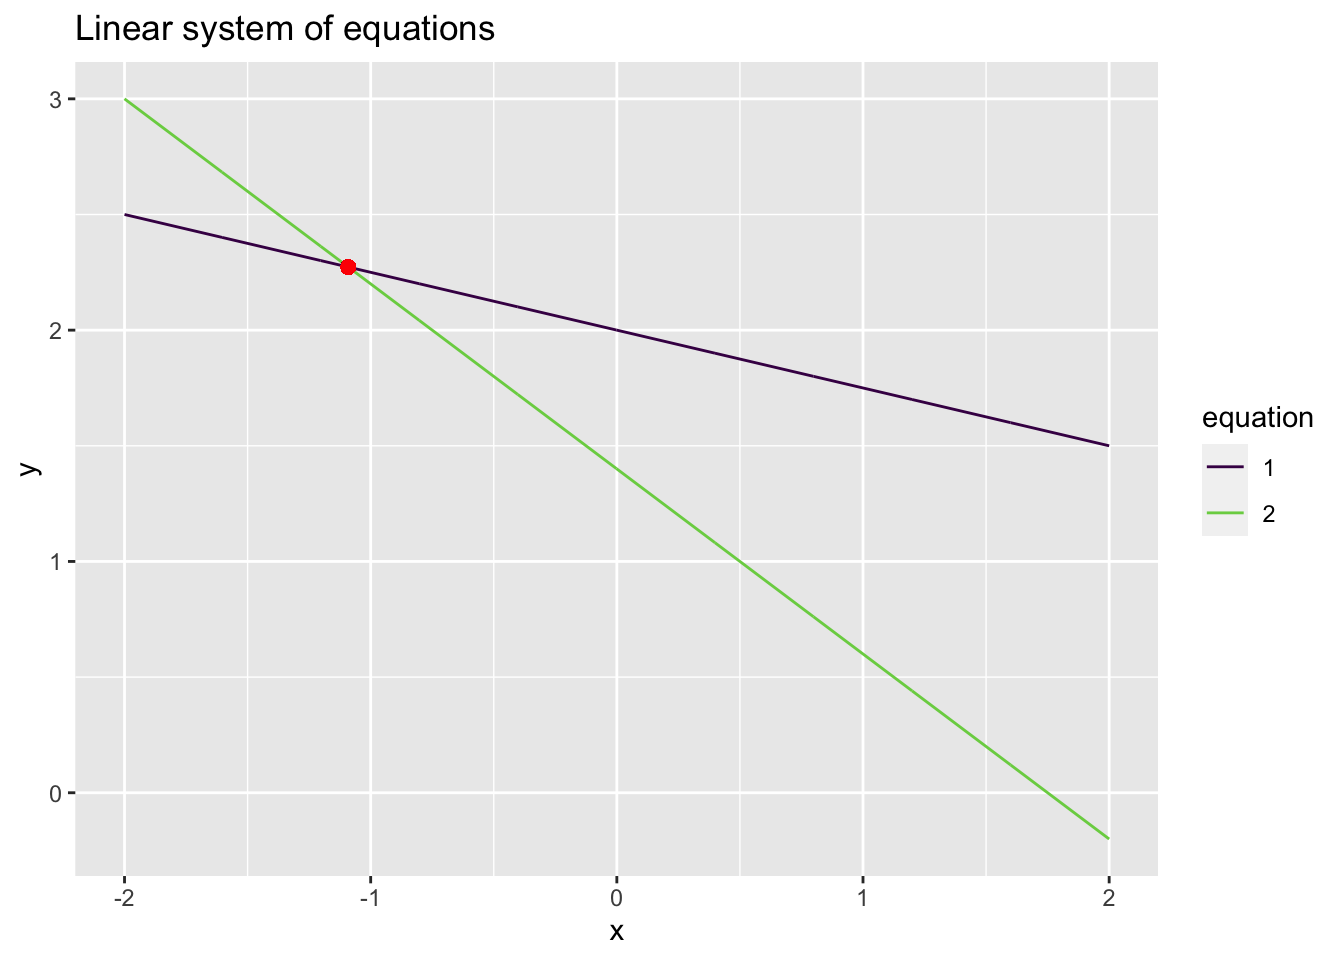
\includegraphics{multivariable-math_files/figure-latex/one-solution-1.pdf}
\caption{\label{fig:one-solution}Linear system of equations with one solution}
\end{figure}

From this plot, it is clear that the solution to the system of equations is the location where the two lines intersect!
\end{solution}

\hypertarget{types-of-solutions}{%
\subsection{Types of solutions}\label{types-of-solutions}}

Typically, there are 3 cases for the solutions to a system of linear equations

\begin{enumerate}
\def\labelenumi{\arabic{enumi})}
\tightlist
\item
  There are no solutions
\item
  There is one solution (Figure \ref{fig:one-solution})
\item
  There are infinitely many solutions
\end{enumerate}

\begin{definition}
A linear system of equations is called \textbf{consistent} if the system has either one or infinitely many solutions and is called \textbf{inconsistent} if the system has no solution.
\end{definition}

\hypertarget{there-are-no-solutions}{%
\subsubsection{There are no solutions:}\label{there-are-no-solutions}}

Consider the system of linear equations

\begin{alignat*}{3}
x   & {}+{} & 4 y & {}={} & 8 \\
4 x & {}+{} & 16 y & {}={} & 18.
\end{alignat*}

\begin{Shaded}
\begin{Highlighting}[]
\CommentTok{# define some grid points to evaluate the line}
\NormalTok{x <-}\StringTok{ }\KeywordTok{seq}\NormalTok{(}\OperatorTok{-}\DecValTok{2}\NormalTok{, }\DecValTok{2}\NormalTok{, }\DataTypeTok{length =} \DecValTok{1000}\NormalTok{)}
\NormalTok{dat <-}\StringTok{ }\KeywordTok{data.frame}\NormalTok{(}
    \DataTypeTok{x =} \KeywordTok{c}\NormalTok{(x, x),}
    \DataTypeTok{y =} \KeywordTok{c}\NormalTok{(}\OperatorTok{-}\NormalTok{x }\OperatorTok{/}\StringTok{ }\DecValTok{4} \OperatorTok{+}\StringTok{ }\DecValTok{8} \OperatorTok{/}\StringTok{ }\DecValTok{4}\NormalTok{, }\OperatorTok{-}\StringTok{ }\NormalTok{x }\OperatorTok{/}\StringTok{ }\DecValTok{4} \OperatorTok{+}\StringTok{ }\DecValTok{18} \OperatorTok{/}\StringTok{ }\DecValTok{4}\NormalTok{),}
    \DataTypeTok{equation =} \KeywordTok{factor}\NormalTok{(}\KeywordTok{rep}\NormalTok{(}\KeywordTok{c}\NormalTok{(}\DecValTok{1}\NormalTok{, }\DecValTok{2}\NormalTok{), }\DataTypeTok{each =} \DecValTok{1000}\NormalTok{))}
\NormalTok{)}
\KeywordTok{glimpse}\NormalTok{(dat)}
\end{Highlighting}
\end{Shaded}

\begin{verbatim}
## Rows: 2,000
## Columns: 3
## $ x        <dbl> -2.000000, -1.995996, -1.991992, -1.987988, -1.983984, -1.979~
## $ y        <dbl> 2.500000, 2.498999, 2.497998, 2.496997, 2.495996, 2.494995, 2~
## $ equation <fct> 1, 1, 1, 1, 1, 1, 1, 1, 1, 1, 1, 1, 1, 1, 1, 1, 1, 1, 1, 1, 1~
\end{verbatim}

\begin{Shaded}
\begin{Highlighting}[]
\NormalTok{dat }\OperatorTok
\StringTok{    }\KeywordTok{ggplot}\NormalTok{(}\KeywordTok{aes}\NormalTok{(}\DataTypeTok{x =}\NormalTok{ x, }\DataTypeTok{y =}\NormalTok{ y, }\DataTypeTok{color =}\NormalTok{ equation, }\DataTypeTok{group =}\NormalTok{ equation)) }\OperatorTok{+}
\StringTok{    }\KeywordTok{geom_line}\NormalTok{() }\OperatorTok{+}
\StringTok{    }\KeywordTok{scale_color_viridis_d}\NormalTok{(}\DataTypeTok{end =} \FloatTok{0.8}\NormalTok{) }\OperatorTok{+}
\StringTok{    }\CommentTok{# solution x = -12/11, y = 25/11}
\StringTok{    }\KeywordTok{ggtitle}\NormalTok{(}\StringTok{"Linear system of equations"}\NormalTok{)}
\end{Highlighting}
\end{Shaded}

\begin{figure}
\centering
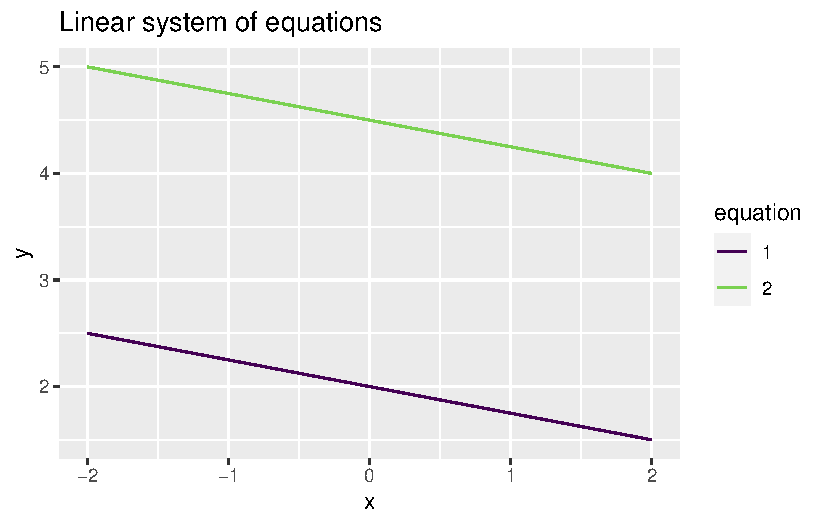
\includegraphics{multivariable-math_files/figure-latex/no-solution-1.pdf}
\caption{\label{fig:no-solution}Linear system of equations with no solution}
\end{figure}

In this case, the linear equations are parallel lines and will never intersect so therefore there is no solution.

\begin{solution}
To find if a solution to this equation exists, we can do some algebra and take 4 times the top equation and then subtract the bottom equation, replacing the bottom equation with this new sum like

\begin{alignat*}{3}
x   & {}+{} & 4 y & {}={} & 8 \\
4 x  - 4(x) & {}+{} & 16 y - 4\times (4 y) & {}={} & 18 - 4 \times (8).
\end{alignat*}

where the part of the equations in \texttt{()} is the top equation. This system of equations now simplifies to

\begin{alignat*}{3}
x & {}+{} & 4 y & {}={} & 8 \\
0 x & {}+{} &  0 y & {}={} & -14,
\end{alignat*}

which gives \(0 = -14\). From this, we see that we have reached a contradiction so there is not a solutoin to the system of equations.
\end{solution}

\hypertarget{there-is-one-solution}{%
\subsubsection{There is one solution:}\label{there-is-one-solution}}

We have seen this example in Figure \ref{fig:one-solution}.

\hypertarget{there-are-infinitely-many-solutions}{%
\subsubsection{There are infinitely many solutions:}\label{there-are-infinitely-many-solutions}}

Consider the system of linear equations

\begin{alignat*}{3}
x   & {}+{} & 4 y & {}={} & 8 \\
4 x & {}+{} & 16 y & {}={} & 32.
\end{alignat*}

\begin{Shaded}
\begin{Highlighting}[]
\CommentTok{# define some grid points to evaluate the line}
\NormalTok{x <-}\StringTok{ }\KeywordTok{seq}\NormalTok{(}\OperatorTok{-}\DecValTok{2}\NormalTok{, }\DecValTok{2}\NormalTok{, }\DataTypeTok{length =} \DecValTok{1000}\NormalTok{)}
\NormalTok{dat <-}\StringTok{ }\KeywordTok{data.frame}\NormalTok{(}
    \DataTypeTok{x =} \KeywordTok{c}\NormalTok{(x, x),}
    \DataTypeTok{y =} \KeywordTok{c}\NormalTok{(}\OperatorTok{-}\NormalTok{x }\OperatorTok{/}\StringTok{ }\DecValTok{4} \OperatorTok{+}\StringTok{ }\DecValTok{8} \OperatorTok{/}\StringTok{ }\DecValTok{4}\NormalTok{, }\OperatorTok{-}\StringTok{ }\DecValTok{4} \OperatorTok{*}\StringTok{ }\NormalTok{x }\OperatorTok{/}\StringTok{ }\DecValTok{16} \OperatorTok{+}\StringTok{ }\DecValTok{32} \OperatorTok{/}\StringTok{ }\DecValTok{16}\NormalTok{),}
    \DataTypeTok{equation =} \KeywordTok{factor}\NormalTok{(}\KeywordTok{rep}\NormalTok{(}\KeywordTok{c}\NormalTok{(}\DecValTok{1}\NormalTok{, }\DecValTok{2}\NormalTok{), }\DataTypeTok{each =} \DecValTok{1000}\NormalTok{))}
\NormalTok{)}
\KeywordTok{glimpse}\NormalTok{(dat)}
\end{Highlighting}
\end{Shaded}

\begin{verbatim}
## Rows: 2,000
## Columns: 3
## $ x        <dbl> -2.000000, -1.995996, -1.991992, -1.987988, -1.983984, -1.979~
## $ y        <dbl> 2.500000, 2.498999, 2.497998, 2.496997, 2.495996, 2.494995, 2~
## $ equation <fct> 1, 1, 1, 1, 1, 1, 1, 1, 1, 1, 1, 1, 1, 1, 1, 1, 1, 1, 1, 1, 1~
\end{verbatim}

\begin{Shaded}
\begin{Highlighting}[]
\NormalTok{dat }\OperatorTok
\StringTok{    }\KeywordTok{ggplot}\NormalTok{(}\KeywordTok{aes}\NormalTok{(}\DataTypeTok{x =}\NormalTok{ x, }\DataTypeTok{y =}\NormalTok{ y, }\DataTypeTok{color =}\NormalTok{ equation, }\DataTypeTok{group =}\NormalTok{ equation)) }\OperatorTok{+}
\StringTok{    }\KeywordTok{geom_line}\NormalTok{() }\OperatorTok{+}
\StringTok{    }\KeywordTok{scale_color_viridis_d}\NormalTok{(}\DataTypeTok{end =} \FloatTok{0.8}\NormalTok{) }\OperatorTok{+}
\StringTok{    }\CommentTok{# solution x = -12/11, y = 25/11}
\StringTok{    }\KeywordTok{ggtitle}\NormalTok{(}\StringTok{"Linear system of equations"}\NormalTok{)}
\end{Highlighting}
\end{Shaded}

\begin{figure}
\centering
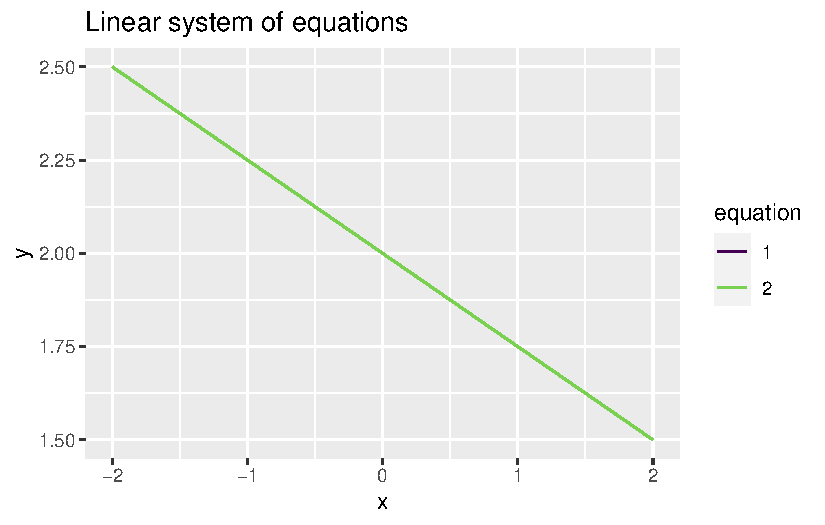
\includegraphics{multivariable-math_files/figure-latex/infinite-solutions-1.pdf}
\caption{\label{fig:infinite-solutions}Linear system of equations with no solution}
\end{figure}

In this case, the linear equations are perfectly overlapping lines and always intersect so therefore there are infinitely many solutions (all points on the line).

\begin{definition}
Two linear systems of equations are called \textbf{equivalent} if both systems share the same \textbf{solution set}.
\end{definition}

For example, the system of equations

\begin{alignat*}{4}
x_1   & {}+{} & 4 x_2 & {}-{} & x_3 & {}={} & 11 \\
4 x_1 & {}+{} & 5 x_2 & {}+{} & 2 x_3 & {}={} & 9
\end{alignat*}

and the system of equations

\begin{alignat*}{4}
2x_1   & {}+{} & 8 x_2 & {}-{} & 2 x_3 & {}={} & 22 \\
8 x_1 & {}+{} & 10 x_2 & {}+{} & 4 x_3 & {}={} & 18.
\end{alignat*}

have the same solution set (the second set of equations is just 2 times the first set of equations).

\begin{example}
For the following system of equations, determine if a solution(s) exist and if so, solve for the solution

\begin{alignat*}{3}
4 x_1 & {}+{} & 5 x_2 & {}={} & 8 \\
9 x_1 & {}-{} & 3 x_2 & {}={} & 4.
\end{alignat*}
\end{example}

\begin{solution}

Multiply the first equation by \(\frac{1}{4}\) and the second equation by \(\frac{1}{9}\) to get

\begin{alignat*}{3}
x_1 & {}+{} & \frac{5}{4} x_2 & {}={} & 2 \\
x_1 & {}-{} &  \frac{1}{3}x_2 & {}={} & \frac{4}{9}.
\end{alignat*}

Subtract the first equation from the second equation

\begin{alignat*}{3}
x_1 & {}+{} & \frac{5}{4} x_2 & {}={} & 2 \\
0 & {}-{} &  (-\frac{1}{3} - \frac{5}{4}) x_2 & {}={} & \frac{4}{9} - 2,
\end{alignat*}
which reduces to
\begin{alignat*}{3}
x_1 & {}+{} & \frac{5}{4} x_2 & {}={} & 2 \\
0 & {}-{} &  -\frac{19}{12} x_2 & {}={} & -\frac{14}{9},
\end{alignat*}

so that, dividing both sides of the second equation by \(-\frac{19}{12}\) gives \(x_2 = \frac{56}{57}\). Plugging this value of \(x_2\) into the first equation gives

\begin{alignat*}{3}
x_1 & {}+{} & \frac{5}{4} \left(\frac{56}{57}\right) & {}={} & 2 \\
0 & {}-{} &   x_2 & {}={} & \frac{56}{57}
\end{alignat*}

and subtracting \(\frac{5}{4} \frac{56}{57}\) from both sides of the first equation gives \(x_1 = \frac{44}{57}\). You can check these solutions by verifying that the following two equations hold

\begin{alignat*}{3}
4 \left(\frac{44}{57}\right) & {}+{} & 5  \left(\frac{56}{57}\right) & {}={} & 8 \\
9 \left(\frac{44}{57}\right) & {}-{} & 3 \left(\frac{56}{57}\right)& {}={} & 4
\end{alignat*}

which can be done in \texttt{R} using

\begin{Shaded}
\begin{Highlighting}[]
\NormalTok{x1 <-}\StringTok{ }\DecValTok{44}\OperatorTok{/}\DecValTok{57}
\NormalTok{x2 <-}\StringTok{ }\DecValTok{56}\OperatorTok{/}\DecValTok{57}
\KeywordTok{all.equal}\NormalTok{(}\DecValTok{4} \OperatorTok{*}\StringTok{ }\NormalTok{x1 }\OperatorTok{+}\StringTok{ }\DecValTok{5} \OperatorTok{*}\StringTok{ }\NormalTok{x2, }\DecValTok{8}\NormalTok{)}
\end{Highlighting}
\end{Shaded}

\begin{verbatim}
## [1] TRUE
\end{verbatim}

\begin{Shaded}
\begin{Highlighting}[]
\KeywordTok{all.equal}\NormalTok{(}\DecValTok{9} \OperatorTok{*}\StringTok{ }\NormalTok{x1 }\OperatorTok{-}\StringTok{ }\DecValTok{3} \OperatorTok{*}\StringTok{ }\NormalTok{x2, }\DecValTok{4}\NormalTok{)}
\end{Highlighting}
\end{Shaded}

\begin{verbatim}
## [1] TRUE
\end{verbatim}

\end{solution}

\begin{example}
For the following system of equations, determine if a solution(s) exist and if so, solve for the solution

\begin{alignat*}{4}
7 x_1 & {}+{} & 3 x_2 & {}+{} & 4 x_3 & {}={} & 5\\
4 x_1 & {}-{} & 5 x_2 &&        & {}={} & -2
\end{alignat*}
\end{example}

\begin{solution}

Multiply the first equation by \(\frac{1}{7}\) and the second equation by \(\frac{1}{4}\) to get

\begin{alignat*}{4}
x_1 & {}+{} & \frac{3}{7} x_2 & {}+{} & \frac{4}{7} x_3 & {}={} & \frac{5}{7} \\
x_1 & {}-{} & \frac{5}{4} x_2 & {}+{} & 0 x_3       & {}={} & \frac{-1}{2}
\end{alignat*}

Subtract the first equation from the second equation

\begin{alignat*}{4}
x_1 & {}+{} & \frac{3}{7} x_2 & {}+{} & \frac{4}{7} x_3 & {}={} & \frac{5}{7} \\
0 x_1 & {}+{} &  (-\frac{5}{4} - \frac{3}{7}) x_2 &{}+{}& -\frac{4}{7} x_3  & {}={} & - \frac{1}{2} - \frac{5}{7}
\end{alignat*}

which reduces to

\begin{alignat*}{4}
x_1 & {}+{} & \frac{3}{7} x_2 & {}+{} & \frac{4}{7} x_3 & {}={} & \frac{5}{7} \\
0 & {}-{} &  -\frac{47}{28} x_2 &{}-{}& \frac{4}{7} x_3 & {}={} & -\frac{17}{14}.
\end{alignat*}

Next, divide the second equation by \(\frac{-47}{28}\) gives

\begin{alignat*}{4}
x_1 & {}+{} & \frac{3}{7} x_2 & {}+{} & \frac{4}{7} x_3 & {}={} & \frac{5}{7} \\
0 & {}+{} & x_2 &{}+{}& \frac{16}{47} x_3 & {}={} & \frac{34}{47}.
\end{alignat*}

Then, take the first equation and subtract \(-\frac{3}{7}\) times the second row to get

\begin{alignat*}{4}
x_1 & {}+{} & 0 x_2 & {}+{} & \frac{20}{47} x_3 & {}={} & \frac{19}{47} \\
0 & {}+{} & x_2 &{}+{}& \frac{16}{47} x_3 & {}={} & \frac{34}{47}.
\end{alignat*}

Which gives the solution
\(x_1 + \frac{20}{47} x_3 = \frac{19}{47}\), \(x_2 + \frac{16}{47} x_3 = \frac{34}{47}\), and \(x_3 = x_3\) is a free variable.

The solution can be checked in \texttt{R} using

\begin{Shaded}
\begin{Highlighting}[]
\CommentTok{# this is a free variable, you can assign it any value}
\NormalTok{x3 <-}\StringTok{ }\DecValTok{3}
\NormalTok{x1 <-}\StringTok{ }\DecValTok{19}\OperatorTok{/}\DecValTok{47} \OperatorTok{-}\StringTok{ }\DecValTok{20}\OperatorTok{/}\DecValTok{47} \OperatorTok{*}\StringTok{ }\NormalTok{x3}
\NormalTok{x2 <-}\StringTok{ }\DecValTok{34}\OperatorTok{/}\DecValTok{47} \OperatorTok{-}\StringTok{ }\DecValTok{16}\OperatorTok{/}\DecValTok{47} \OperatorTok{*}\StringTok{ }\NormalTok{x3}
\CommentTok{# check the first equation}
\KeywordTok{all.equal}\NormalTok{(}\DecValTok{7} \OperatorTok{*}\StringTok{ }\NormalTok{x1 }\OperatorTok{+}\StringTok{ }\DecValTok{3} \OperatorTok{*}\StringTok{ }\NormalTok{x2 }\OperatorTok{+}\StringTok{ }\DecValTok{4} \OperatorTok{*}\StringTok{ }\NormalTok{x3, }\DecValTok{5}\NormalTok{)}
\end{Highlighting}
\end{Shaded}

\begin{verbatim}
## [1] TRUE
\end{verbatim}

\begin{Shaded}
\begin{Highlighting}[]
\CommentTok{# check the second equation}
\KeywordTok{all.equal}\NormalTok{(}\DecValTok{4} \OperatorTok{*}\StringTok{ }\NormalTok{x1 }\OperatorTok{-}\StringTok{ }\DecValTok{5} \OperatorTok{*}\StringTok{ }\NormalTok{x2 }\OperatorTok{+}\StringTok{ }\DecValTok{0} \OperatorTok{*}\StringTok{ }\NormalTok{x3, }\DecValTok{-2}\NormalTok{)}
\end{Highlighting}
\end{Shaded}

\begin{verbatim}
## [1] TRUE
\end{verbatim}

\end{solution}

\begin{example}
For the following system of equations, determine if a solution(s) exist and if so, solve for the solution

\begin{alignat*}{3}
4 x_1 & {}-{} & 2 x_2 & {}={} & 8\\
2 x_1 & {}+{} & x_2 & {}={} & 7 \\
-3 x_1 & {}+{} & 6 x_2 &{}={} & 11
\end{alignat*}
\end{example}

\begin{solution}
Multiply the first equation by \(\frac{1}{4}\), the second equation by \(\frac{1}{2}\), and the third equation by \(-\frac{1}{3}\) to get

\begin{alignat*}{3}
x_1 & {}-{} & \frac{1}{2} x_2 & {}={} & 2\\
x_1 & {}+{} & \frac{1}{2} x_2 & {}={} & \frac{7}{2} \\
 x_1 & {}-{} & 2 x_2 &{}={} & -\frac{11}{3}
\end{alignat*}

Subtract the first equation from the second equation and also subtract the first equation from the third equation. Thus, we get

\begin{alignat*}{3}
x_1 & {}-{} & \frac{1}{2} x_2 & {}={} & 2\\
0 x_1 & {}+{} & x_2 & {}={} & \frac{3}{2} \\
0 x_1 & {}-{} & \frac{3}{2} x_2 &{}={} & -\frac{17}{3}.
\end{alignat*}

Then, multiply the third equation by \(-\frac{2}{3}\) to get

\begin{alignat*}{3}
x_1 & {}-{} & \frac{1}{2} x_2 & {}={} & 2\\
0 x_1 & {}+{} & x_2 & {}={} & 3 \\
0 x_1 & {}+{} & x_2 &{}={} & - \frac{34}{9}.
\end{alignat*}

Notice that the second equation gives \(x_2 = 3\) while the third equation gives \(x_2 = -\frac{34}{9}\). This is a contradiction (\(3 \neq -\frac{34}{9})\) which implies that the system of equations does not have a solution. Thus we say the system of equations is inconsistent.
\end{solution}

\hypertarget{elementary-row-and-column-operations-on-matrices}{%
\subsection{Elementary row and column operations on matrices}\label{elementary-row-and-column-operations-on-matrices}}

The elementary row (column) operations include

\begin{enumerate}
\def\labelenumi{\arabic{enumi})}
\tightlist
\item
  swaps: swapping two rows (columns),
\item
  sums: replacing a row (column) by the sum itself and a multiple of another row (column)
\item
  scalar multiplication: replacing a row (column) by a scalar multiple times itself
\end{enumerate}

Note that these operations are exactly what we used to solve the equation using algebra above (except for swapping rows).

\begin{example}

For the elementary row operations listed above, we demonstrate these using the matrix

\[
\begin{aligned}
\begin{pmatrix} 1 & 4 & 7 \\ 2 & 5 & 8 \\ 3 & 6 & 9 \end{pmatrix}
\end{aligned}
\]

The matrix \(\mathbf{A}\) can be represented in \texttt{R} using

\begin{Shaded}
\begin{Highlighting}[]
\NormalTok{A <-}\StringTok{ }\KeywordTok{matrix}\NormalTok{(}\KeywordTok{c}\NormalTok{(}\DecValTok{1}\OperatorTok{:}\DecValTok{9}\NormalTok{), }\DecValTok{3}\NormalTok{, }\DecValTok{3}\NormalTok{, }\DataTypeTok{byrow =} \OtherTok{FALSE}\NormalTok{)}
\end{Highlighting}
\end{Shaded}

\begin{enumerate}
\def\labelenumi{\arabic{enumi})}
\item
  Swap the first and second rows.
\item
  Add -3 times the first row to the third row.
\item
  Multiply the second row by \(\frac{1}{2}\).
\end{enumerate}

\end{example}

\begin{solution}

Here we present examples of the elementary row operations

\begin{enumerate}
\def\labelenumi{\arabic{enumi})}
\tightlist
\item
  Swap the first and second rows.
\end{enumerate}

The matrix with the first and second rows swapped is

\[
\begin{aligned}
\begin{pmatrix} 2 & 5 & 8 \\ 1 & 4 & 7 \end{pmatrix}
\end{aligned}
\]

Notice that the first and second rows have now switched places. This can be done in \texttt{R} in a variety of ways. First, we extract the rows and place them ``by hand'' in \texttt{R}.

\begin{Shaded}
\begin{Highlighting}[]
\NormalTok{A <-}\StringTok{ }\KeywordTok{matrix}\NormalTok{(}\KeywordTok{c}\NormalTok{(}\DecValTok{1}\OperatorTok{:}\DecValTok{9}\NormalTok{), }\DecValTok{3}\NormalTok{, }\DecValTok{3}\NormalTok{, }\DataTypeTok{byrow =} \OtherTok{FALSE}\NormalTok{)}
\CommentTok{# extract the rows}
\NormalTok{row1 <-}\StringTok{ }\NormalTok{A[}\DecValTok{1}\NormalTok{, ] }
\NormalTok{row2 <-}\StringTok{ }\NormalTok{A[}\DecValTok{2}\NormalTok{, ]}
\CommentTok{# swap the rows}
\NormalTok{A[}\DecValTok{1}\NormalTok{, ] <-}\StringTok{ }\NormalTok{row2}
\NormalTok{A[}\DecValTok{2}\NormalTok{, ] <-}\StringTok{ }\NormalTok{row1}
\NormalTok{A}
\end{Highlighting}
\end{Shaded}

\begin{verbatim}
##      [,1] [,2] [,3]
## [1,]    2    5    8
## [2,]    1    4    7
## [3,]    3    6    9
\end{verbatim}

Another way to do this is to use the function \texttt{rbind()} that binds rows together into a matrix.

\begin{Shaded}
\begin{Highlighting}[]
\NormalTok{A <-}\StringTok{ }\KeywordTok{matrix}\NormalTok{(}\KeywordTok{c}\NormalTok{(}\DecValTok{1}\OperatorTok{:}\DecValTok{9}\NormalTok{), }\DecValTok{3}\NormalTok{, }\DecValTok{3}\NormalTok{, }\DataTypeTok{byrow =} \OtherTok{FALSE}\NormalTok{)}
\CommentTok{# bind row 2, row 1, and row 3 togethter}
\KeywordTok{rbind}\NormalTok{(A[}\DecValTok{2}\NormalTok{, ], A[}\DecValTok{1}\NormalTok{, ], A[}\DecValTok{3}\NormalTok{, ])}
\end{Highlighting}
\end{Shaded}

\begin{verbatim}
##      [,1] [,2] [,3]
## [1,]    2    5    8
## [2,]    1    4    7
## [3,]    3    6    9
\end{verbatim}

Yet another way to swap the first two rows is to use a vectorized operation. This allows for fast and efficient coding and computing. The vectorized row swap is

\begin{Shaded}
\begin{Highlighting}[]
\NormalTok{A <-}\StringTok{ }\KeywordTok{matrix}\NormalTok{(}\KeywordTok{c}\NormalTok{(}\DecValTok{1}\OperatorTok{:}\DecValTok{9}\NormalTok{), }\DecValTok{3}\NormalTok{, }\DecValTok{3}\NormalTok{, }\DataTypeTok{byrow =} \OtherTok{FALSE}\NormalTok{)}
\CommentTok{# Take the 2nd, 1st, and 3rd row of A, in that order}
\NormalTok{A[}\KeywordTok{c}\NormalTok{(}\DecValTok{2}\NormalTok{, }\DecValTok{1}\NormalTok{, }\DecValTok{3}\NormalTok{), ]}
\end{Highlighting}
\end{Shaded}

\begin{verbatim}
##      [,1] [,2] [,3]
## [1,]    2    5    8
## [2,]    1    4    7
## [3,]    3    6    9
\end{verbatim}

\begin{enumerate}
\def\labelenumi{\arabic{enumi})}
\setcounter{enumi}{1}
\tightlist
\item
  Add -3 times the first row to the third row.
\end{enumerate}

First, we notice that -3 times the first row gives the row vector \(\begin{pmatrix} -3 & -12 & -21 \end{pmatrix}\). Then, we add this to the row vector of the third row \(\begin{pmatrix} 3 & 6 & 9 \end{pmatrix}\) to get the row vector \(\begin{pmatrix} 0 & -6 & -12 \end{pmatrix}\). Finally, this row vector replaces the third row of the matrix to give the result
\[
\begin{aligned}
\begin{pmatrix} 1 & 4 & 7 \\ 2 & 5 & 8 \\ 0 & -6 & -12 \end{pmatrix}
\end{aligned}
\]

\textbf{Note:} Notice that by performing this row sum and replacement, we have made the first column of the third row of \(\mathbf{A}\) a 0. This zeroing out of the columns will play a very important role moving forward.

Using \texttt{R}, this can be done as

\begin{Shaded}
\begin{Highlighting}[]
\NormalTok{A <-}\StringTok{ }\KeywordTok{matrix}\NormalTok{(}\KeywordTok{c}\NormalTok{(}\DecValTok{1}\OperatorTok{:}\DecValTok{9}\NormalTok{), }\DecValTok{3}\NormalTok{, }\DecValTok{3}\NormalTok{, }\DataTypeTok{byrow =} \OtherTok{FALSE}\NormalTok{)}
\CommentTok{# extract the rows }
\NormalTok{row1 <-}\StringTok{ }\NormalTok{A[}\DecValTok{1}\NormalTok{, ]}
\NormalTok{row3 <-}\StringTok{ }\NormalTok{A[}\DecValTok{3}\NormalTok{, ]}
\NormalTok{A[}\DecValTok{3}\NormalTok{, ] <-}\StringTok{ }\DecValTok{-3} \OperatorTok{*}\StringTok{ }\NormalTok{row1 }\OperatorTok{+}\StringTok{ }\NormalTok{row3}
\NormalTok{A}
\end{Highlighting}
\end{Shaded}

\begin{verbatim}
##      [,1] [,2] [,3]
## [1,]    1    4    7
## [2,]    2    5    8
## [3,]    0   -6  -12
\end{verbatim}

Another way to do this row sum and replacement is

\begin{Shaded}
\begin{Highlighting}[]
\NormalTok{A <-}\StringTok{ }\KeywordTok{matrix}\NormalTok{(}\KeywordTok{c}\NormalTok{(}\DecValTok{1}\OperatorTok{:}\DecValTok{9}\NormalTok{), }\DecValTok{3}\NormalTok{, }\DecValTok{3}\NormalTok{, }\DataTypeTok{byrow =} \OtherTok{FALSE}\NormalTok{)}
\NormalTok{A[}\DecValTok{3}\NormalTok{, ] <-}\StringTok{ }\DecValTok{-3} \OperatorTok{*}\StringTok{ }\NormalTok{A[}\DecValTok{1}\NormalTok{, ] }\OperatorTok{+}\StringTok{ }\NormalTok{A[}\DecValTok{3}\NormalTok{, ]}
\NormalTok{A}
\end{Highlighting}
\end{Shaded}

\begin{verbatim}
##      [,1] [,2] [,3]
## [1,]    1    4    7
## [2,]    2    5    8
## [3,]    0   -6  -12
\end{verbatim}

\begin{enumerate}
\def\labelenumi{\arabic{enumi})}
\setcounter{enumi}{2}
\tightlist
\item
  Multiply the second row by \(\frac{1}{2}\).
\end{enumerate}

The second row of \(\mathbf{A}\) is the row vector \(\begin{pmatrix} 2 & 5 & 8 \end{pmatrix}\). Multiplying the second row by \(\frac{1}{2}\) gives the row vector \(\begin{pmatrix} 1 & 5/2 & 4 \end{pmatrix}\). Plugging this into the matrix gives the full matrix with second row multiplied by \(\frac{1}{2}\) as
\[
\begin{aligned}
\begin{pmatrix} 1 & 4 & 7 \\ 1 & 5/2 & 4 \\ 3 & 6 & 9 \end{pmatrix}
\end{aligned}
\]
In \texttt{R}, the second row of \(\mathbf{A}\) can be multiplied by \(\frac{1}{2}\) as

\begin{Shaded}
\begin{Highlighting}[]
\NormalTok{A[}\DecValTok{2}\NormalTok{, ] <-}\StringTok{ }\DecValTok{1}\OperatorTok{/}\DecValTok{2} \OperatorTok{*}\StringTok{ }\NormalTok{A[}\DecValTok{2}\NormalTok{, ]}
\NormalTok{A}
\end{Highlighting}
\end{Shaded}

\begin{verbatim}
##      [,1] [,2] [,3]
## [1,]    1  4.0    7
## [2,]    1  2.5    4
## [3,]    3  6.0    9
\end{verbatim}

\end{solution}

\hypertarget{the-augmented-matrix-form-of-a-system-of-equations}{%
\subsection{The Augmented matrix form of a system of equations}\label{the-augmented-matrix-form-of-a-system-of-equations}}

Consider the linear system of equations

\begin{alignat*}{4}
x_1   & {}+{} & 4 x_2 & {}-{} & x_3 & {}={} & 11 \\
4 x_1 & {}+{} & 5 x_2 & {}+{} & 2 x_3 & {}={} & 9.
\end{alignat*}

The augmented matrix representation of this system of linear equations is given by the matrix
\[
\begin{aligned}
\begin{pmatrix}
1 & 4 & - 1 & 11 \\
4 & 5 & 2   &  9
\end{pmatrix},
\end{aligned}
\]
where the first column of the matrix represents the variable \(x_1\), the second column of the matrix represents the variable \(x_2\), the third column of the matrix represents the variable \(x_3\), and the fourth column of the matrix represents the constant terms. We can express the augmented form in \texttt{R} using a matrix

\begin{Shaded}
\begin{Highlighting}[]
\NormalTok{augmented_matrix <-}\StringTok{ }\KeywordTok{matrix}\NormalTok{(}\KeywordTok{c}\NormalTok{(}\DecValTok{1}\NormalTok{, }\DecValTok{4}\NormalTok{, }\DecValTok{4}\NormalTok{, }\DecValTok{5}\NormalTok{, }\DecValTok{-1}\NormalTok{, }\DecValTok{2}\NormalTok{, }\DecValTok{11}\NormalTok{, }\DecValTok{9}\NormalTok{), }\DecValTok{2}\NormalTok{, }\DecValTok{4}\NormalTok{)}
\NormalTok{augmented_matrix}
\end{Highlighting}
\end{Shaded}

\begin{verbatim}
##      [,1] [,2] [,3] [,4]
## [1,]    1    4   -1   11
## [2,]    4    5    2    9
\end{verbatim}

and to make clear the respective variables, we can add in column names as a matrix attribute using the \texttt{colnames()} function

\begin{Shaded}
\begin{Highlighting}[]
\KeywordTok{colnames}\NormalTok{(augmented_matrix) <-}\StringTok{ }\KeywordTok{c}\NormalTok{(}\StringTok{"x1"}\NormalTok{, }\StringTok{"x2"}\NormalTok{, }\StringTok{"x3"}\NormalTok{, }\StringTok{"constants"}\NormalTok{)}
\NormalTok{augmented_matrix}
\end{Highlighting}
\end{Shaded}

\begin{verbatim}
##      x1 x2 x3 constants
## [1,]  1  4 -1        11
## [2,]  4  5  2         9
\end{verbatim}

which adds labels to each of the columns.

Now, using elementary row operations on the matrix, we can attempt to find solutions to the system of equations. First, we multiply the first row by -4 and add it to the second row of the matrix and replace the second row with this sum

\begin{Shaded}
\begin{Highlighting}[]
\NormalTok{augmented_matrix[}\DecValTok{2}\NormalTok{, ] <-}\StringTok{ }\DecValTok{-4} \OperatorTok{*}\StringTok{ }\NormalTok{augmented_matrix[}\DecValTok{1}\NormalTok{, ] }\OperatorTok{+}\StringTok{ }\NormalTok{augmented_matrix[}\DecValTok{2}\NormalTok{, ]}
\NormalTok{augmented_matrix}
\end{Highlighting}
\end{Shaded}

\begin{verbatim}
##      x1  x2 x3 constants
## [1,]  1   4 -1        11
## [2,]  0 -11  6       -35
\end{verbatim}

Next, scale the second row to have a leading value of 1 by dividing by -11

\begin{Shaded}
\begin{Highlighting}[]
\NormalTok{augmented_matrix[}\DecValTok{2}\NormalTok{, ] <-}\StringTok{ }\NormalTok{augmented_matrix[}\DecValTok{2}\NormalTok{, ] }\OperatorTok{/}\StringTok{ }\NormalTok{(}\OperatorTok{-}\DecValTok{11}\NormalTok{)}
\NormalTok{augmented_matrix}
\end{Highlighting}
\end{Shaded}

\begin{verbatim}
##      x1 x2         x3 constants
## [1,]  1  4 -1.0000000 11.000000
## [2,]  0  1 -0.5454545  3.181818
\end{verbatim}

We can then multiply the second row by -4 and add it to the first row and replace the first row with this value.

\begin{Shaded}
\begin{Highlighting}[]
\NormalTok{augmented_matrix[}\DecValTok{1}\NormalTok{, ] <-}\StringTok{ }\NormalTok{augmented_matrix[}\DecValTok{1}\NormalTok{, ] }\OperatorTok{-}\StringTok{ }\DecValTok{4} \OperatorTok{*}\StringTok{ }\NormalTok{augmented_matrix[}\DecValTok{2}\NormalTok{, ]}
\NormalTok{augmented_matrix}
\end{Highlighting}
\end{Shaded}

\begin{verbatim}
##      x1 x2         x3 constants
## [1,]  1  0  1.1818182 -1.727273
## [2,]  0  1 -0.5454545  3.181818
\end{verbatim}

Notice how the matrix has a ``triangular'' form (The lower part of the ``triangle'' is made of 0s and the upper part has numbers).

The triangular form tells us that There are infinitely many solutions to this system of equation. The infinite solutions are subject to the requirements that
\[x_1 = - \frac{19}{11} - \frac{13}{11} x_3\]
and
\[x_2 = \frac{35}{11} + \frac{6}{11} x_3.\]
To get this into a reasonable form, we will solve these equations as a function of \(x_1\). Solving the first equation for \(x_3\) gives
\[x_3 = - \frac{19}{13} -\frac{11}{13} x_1.\]
Then, plugging this into \(x_3\) in the second equation gives
\[
\begin{aligned}
x_2 & = \frac{35}{11} + \frac{6}{11} \left( - \frac{19}{13} -\frac{11}{13} x_1 \right) \\
& = \frac{341}{143} - \frac{6}{13} x_1
\end{aligned}
\]
which defines a linear relationship between \(x_1\) and \(x_2\). Notice that in these last two solutions, \(x_1\) is a ``free variable'' and \(x_2\) and \(x_3\) are ``determined'' by \(x_1\).

In the plot below, the two planes (red and blue) are the geometric plots of the linear equations in the system of equations (the red plane is the top equation and the blue plane is the bottom equation). The purple line is the equation for the solution given the free variable \(x_3\) and lies at the intersection of the two planes, much like the point in the two lines in figure \textbf{linking reference here} lies at the intersection of the two points.

\begin{Shaded}
\begin{Highlighting}[]
\CommentTok{# uses gg3D library}
\NormalTok{n <-}\StringTok{ }\DecValTok{60}
\NormalTok{x1 <-}\StringTok{ }\NormalTok{x2 <-}\StringTok{ }\KeywordTok{seq}\NormalTok{(}\OperatorTok{-}\DecValTok{10}\NormalTok{, }\DecValTok{10}\NormalTok{, }\DataTypeTok{length =}\NormalTok{ n)}
\NormalTok{region <-}\StringTok{ }\KeywordTok{expand.grid}\NormalTok{(}\DataTypeTok{x1 =}\NormalTok{ x1, }\DataTypeTok{x2 =}\NormalTok{ x2)}
\NormalTok{df <-}\StringTok{ }\KeywordTok{data.frame}\NormalTok{(}
    \DataTypeTok{x1 =}\NormalTok{ region}\OperatorTok{$}\NormalTok{x1,}
    \DataTypeTok{x2 =}\NormalTok{ region}\OperatorTok{$}\NormalTok{x2,}
    \DataTypeTok{x3 =} \OperatorTok{-}\StringTok{ }\DecValTok{11} \OperatorTok{+}\StringTok{ }\NormalTok{(region}\OperatorTok{$}\NormalTok{x1 }\OperatorTok{+}\StringTok{ }\DecValTok{4} \OperatorTok{*}\StringTok{ }\NormalTok{region}\OperatorTok{$}\NormalTok{x2)}
\NormalTok{)}

\NormalTok{df2 <-}\StringTok{ }\KeywordTok{data.frame}\NormalTok{(}
    \DataTypeTok{x1 =}\NormalTok{ region}\OperatorTok{$}\NormalTok{x1,}
    \DataTypeTok{x2 =}\NormalTok{ region}\OperatorTok{$}\NormalTok{x2,}
    \DataTypeTok{x3 =}\NormalTok{ (}\DecValTok{9} \OperatorTok{-}\StringTok{ }\DecValTok{4} \OperatorTok{*}\StringTok{ }\NormalTok{region}\OperatorTok{$}\NormalTok{x1 }\OperatorTok{-}\StringTok{ }\DecValTok{5} \OperatorTok{*}\StringTok{ }\NormalTok{region}\OperatorTok{$}\NormalTok{x2) }\OperatorTok{/}\StringTok{ }\DecValTok{2}
\NormalTok{) }

\NormalTok{df_solution <-}\StringTok{ }\KeywordTok{data.frame}\NormalTok{(}
    \DataTypeTok{x1 =}\NormalTok{ x1, }
    \DataTypeTok{x2 =} \DecValTok{341} \OperatorTok{/}\StringTok{ }\DecValTok{143} \OperatorTok{-}\StringTok{ }\DecValTok{6} \OperatorTok{/}\StringTok{ }\DecValTok{13} \OperatorTok{*}\StringTok{ }\NormalTok{x1,}
    \DataTypeTok{x3 =} \DecValTok{-19}\OperatorTok{/}\DecValTok{13} \OperatorTok{-}\StringTok{ }\DecValTok{11}\OperatorTok{/}\DecValTok{13} \OperatorTok{*}\StringTok{ }\NormalTok{x1}
\NormalTok{) }

\CommentTok{# theta and phi set up the "perspective/viewing angle" of the 3D plot}
\NormalTok{theta <-}\StringTok{ }\DecValTok{63}
\NormalTok{phi <-}\StringTok{ }\DecValTok{-12}
\KeywordTok{ggplot}\NormalTok{(df, }\KeywordTok{aes}\NormalTok{(x1, x2, }\DataTypeTok{z =}\NormalTok{ x3)) }\OperatorTok{+}
\StringTok{    }\KeywordTok{axes_3D}\NormalTok{(}\DataTypeTok{theta =}\NormalTok{ theta, }\DataTypeTok{phi =}\NormalTok{ phi) }\OperatorTok{+}
\StringTok{    }\KeywordTok{stat_wireframe}\NormalTok{(}\DataTypeTok{alpha =} \FloatTok{0.25}\NormalTok{, }\DataTypeTok{color =} \StringTok{"red"}\NormalTok{, }\DataTypeTok{theta =}\NormalTok{ theta, }\DataTypeTok{phi =}\NormalTok{ phi) }\OperatorTok{+}
\StringTok{    }\KeywordTok{stat_wireframe}\NormalTok{(}\DataTypeTok{data =}\NormalTok{ df2, }\KeywordTok{aes}\NormalTok{(}\DataTypeTok{x =}\NormalTok{ x1, }\DataTypeTok{y =}\NormalTok{ x2, }\DataTypeTok{z =}\NormalTok{ x3), }\DataTypeTok{alpha =} \FloatTok{0.25}\NormalTok{, }\DataTypeTok{color =} \StringTok{"blue"}\NormalTok{, }\DataTypeTok{theta =}\NormalTok{ theta, }\DataTypeTok{phi =}\NormalTok{ phi) }\OperatorTok{+}
\StringTok{    }\KeywordTok{stat_3D}\NormalTok{(}\DataTypeTok{data =}\NormalTok{ df_solution, }\KeywordTok{aes}\NormalTok{(x1, x2, }\DataTypeTok{z =}\NormalTok{ x3), }\DataTypeTok{geom =} \StringTok{"line"}\NormalTok{, }\DataTypeTok{theta =}\NormalTok{ theta, }\DataTypeTok{phi =}\NormalTok{ phi, }\DataTypeTok{color =} \StringTok{"purple"}\NormalTok{) }\OperatorTok{+}
\StringTok{    }\KeywordTok{theme_void}\NormalTok{() }\OperatorTok{+}
\StringTok{    }\KeywordTok{theme}\NormalTok{(}\DataTypeTok{legend.position =} \StringTok{"none"}\NormalTok{) }\OperatorTok{+}
\StringTok{    }\KeywordTok{labs_3D}\NormalTok{(}\DataTypeTok{hjust=}\KeywordTok{c}\NormalTok{(}\DecValTok{0}\NormalTok{,}\DecValTok{1}\NormalTok{,}\DecValTok{1}\NormalTok{), }\DataTypeTok{vjust=}\KeywordTok{c}\NormalTok{(}\DecValTok{1}\NormalTok{, }\DecValTok{1}\NormalTok{, }\FloatTok{-0.2}\NormalTok{), }\DataTypeTok{angle=}\KeywordTok{c}\NormalTok{(}\DecValTok{0}\NormalTok{, }\DecValTok{0}\NormalTok{, }\DecValTok{90}\NormalTok{), }\DataTypeTok{theta =}\NormalTok{ theta, }\DataTypeTok{phi =}\NormalTok{ phi) }
\end{Highlighting}
\end{Shaded}

\begin{verbatim}
## Warning: Removed 2 row(s) containing missing values (geom_path).

## Warning: Removed 2 row(s) containing missing values (geom_path).
\end{verbatim}

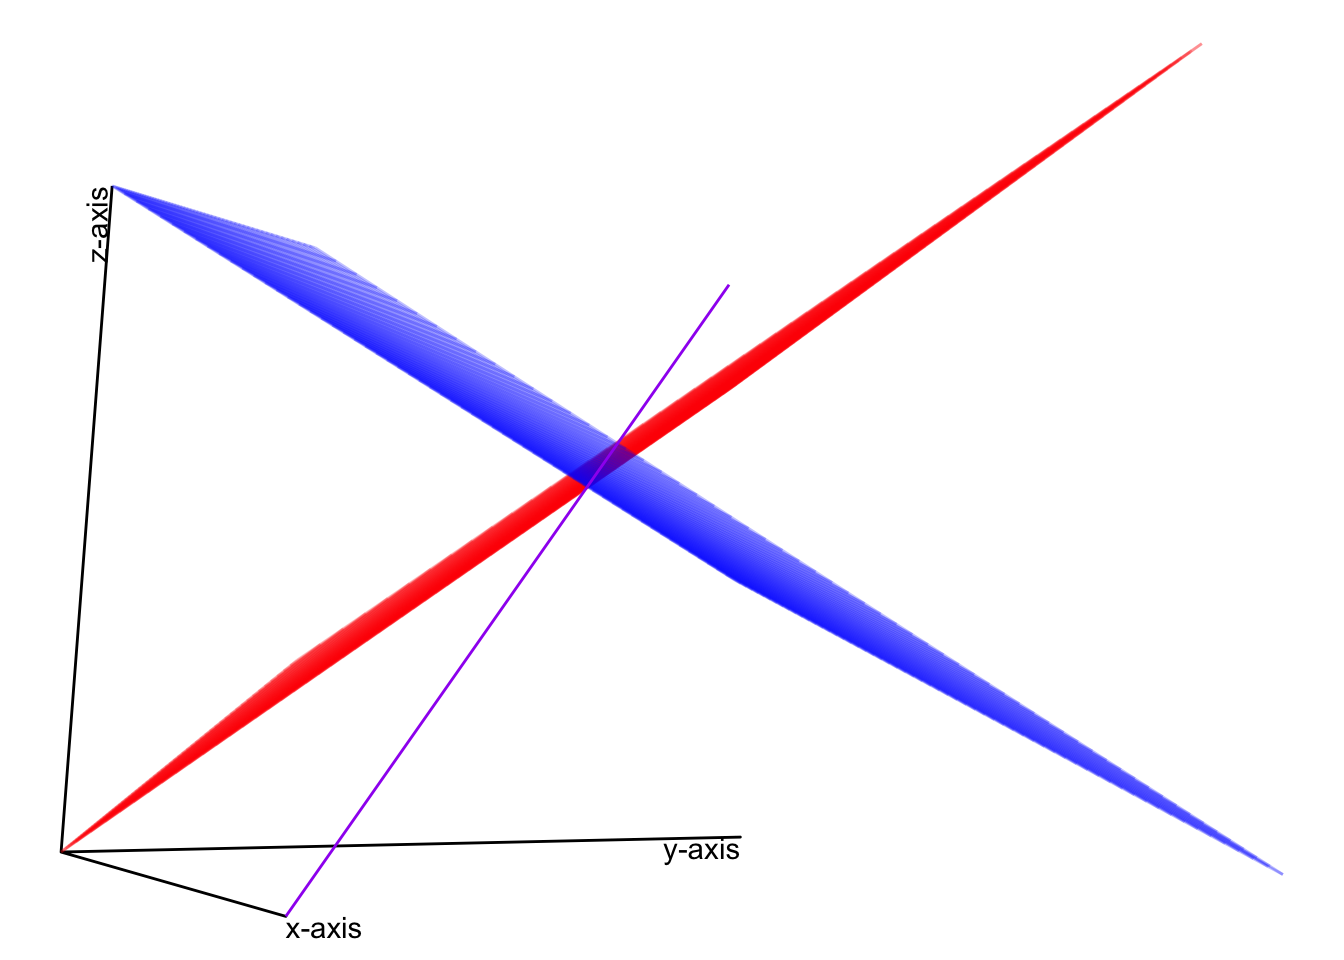
\includegraphics{multivariable-math_files/figure-latex/unnamed-chunk-38-1.pdf}

\hypertarget{existence-and-uniqueness}{%
\subsection{Existence and Uniqueness}\label{existence-and-uniqueness}}

\begin{definition}
A system of linear equations is said to be consistent if at least one solution exists. The linear system of equations is said to have a \textbf{unique} solution if only one solution exists.
\end{definition}

\begin{example}
Is the system of linear equations consistent? If the system is consistent, does it have a unique solution?

\[
\begin{alignedat}{4}  16 x_1 & {}+{} & 2 x_2 & {}+{} & 3 x_3 & {}={} & 13\\ 5 x_1 & {}+{} & 11 x_2 & {}+{} & 10 x_3 & {}={} & 8\\ 9 x_1 & {}+{} & 7 x_2 & {}+{} & 6 x_3 & {}={} & 12\\ 4 x_1 & {}+{} & 14 x_2 & {}+{} & 15 x_3 & {}={} & 1 \end{alignedat}
\]
\end{example}

\begin{solution}
\textbf{fill in solution here}
\end{solution}

\begin{example}
Is the system of linear equations consistent? If the system is consistent, does it have a unique solution?

\[
\begin{alignedat}{4}   x_1 & {}+{} & 2 x_2 & {}+{} & 3 x_3 & {}={} & 5\\  x_1 & {}+{} & 3 x_2 & {}+{} & 2 x_3 & {}={} & 2\\ 3 x_1 & {}+{} & 2 x_2 & {}+{} &  x_3 & {}={} & 7 \end{alignedat}
\]
\end{example}

\begin{solution}
\textbf{fill in solution here}
\end{solution}

\hypertarget{reduce-row-echelon-form}{%
\section{Reduce row echelon form}\label{reduce-row-echelon-form}}

Reducing a matrix to row echelon form is a useful technique for working with matrices. The row echelon form can be used to solve systems of equations, as well as determine other properties of a matrix that are yet to be discussed, including rank, invertibility, column/row spaces, etc.

\begin{definition}

A matrix is said to be in \textbf{echelon} form if

\begin{enumerate}
\def\labelenumi{\arabic{enumi})}
\item
  all nonzero rows are above any rows of zeros (all rows consisting entirely of zeros are at the bottom)
\item
  the leading entry/coefficient of a nonzero row (called the \textbf{pivot}) is always \emph{strictly} to the right of the leading entry/coefficient of the row above
\end{enumerate}

\end{definition}

\begin{example}
\textbf{echelon matrix example in class}
\end{example}

\begin{definition}

A matrix is in \textbf{reduced row echelon form} if it is in echelon form and

\begin{enumerate}
\def\labelenumi{\arabic{enumi})}
\item
  the leading entry/coefficient of each row is 1
\item
  The leading entry/coefficient of 1 is the only nonzero entry in its column.
\end{enumerate}

\end{definition}

\begin{example}
\textbf{rref matrix example in class}
\end{example}

\begin{definition}
Echelon matrices have the property of being \textbf{upper diagonal}. A matrix is said to be \textbf{upper diagonal} if all entries of the matrix at or above the diagonal are nonzero.
\end{definition}

\begin{itemize}
\tightlist
\item
  Example: **lower and non-lower diagonal matrices
\end{itemize}

\begin{definition}
Two matrices are \textbf{row-equivalent} if one matrix can be transformed to the other through elementary row operations.
\end{definition}

\begin{theorem}
A nonzero matrix can be transformed into more than one echelon forms. However, the reduced row echelon form of a nonzero matrix is unique.
\end{theorem}

:::\{.exercise\}

Using elementary row operations, calculate the reduced row echelon form of the following matrices
1) \textbf{fill in later}
2) \textbf{fill in later}
3) \textbf{fill in later}

:::`

\hypertarget{pivot-positions}{%
\subsection{Pivot positions}\label{pivot-positions}}

The leading entry/coefficients of a row echelon form matrix are called pivots. The positions of the pivot positions are the same for any row echelon form of a matrix. In reduced row echelon form, these pivot positions take the value 1.

\begin{definition}
In a matrix that is in reduced echelon form, the pivot position is the first nonzero element of each row. The column in which the pivot position occurs is called a pivot column.
\end{definition}

\begin{example}
\textbf{pivot position and pivot columns}
\end{example}

\hypertarget{finding-the-reduced-row-echelon-form}{%
\subsection{Finding the reduced row echelon form}\label{finding-the-reduced-row-echelon-form}}

Calculating the reduced row echelon form is known as Gaussian elimination, which is named after \href{https://en.wikipedia.org/wiki/Carl_Friedrich_Gauss}{Johann Carl Friedrich Gauss}. This algorithm uses elementary row operations to calculate the reduced row echelon form. The following steps perform the Gaussian elimination algorithm.

\begin{enumerate}
\def\labelenumi{\arabic{enumi})}
\tightlist
\item
  Start with the left-most nonzero column, which is a pivot column
\item
  If the top row is zero, swap rows so that the top row is nonzero so that the top row has a nonzero element in the pivot position.
\item
  Use row multiplication and addition to zero out all positions in the pivot column below the top row (pivot position).
\item
  Ignore this top row and repeat steps 1-3 until there are no more nonzero rows to apply steps 1-3 on. At the end of this step, the matrix is in row echelon form.
\item
  Starting at the right-most pivot column, use elementary row operations to zero out all positions above each pivot and to make each pivot position 1. At the end of this step, the matrix is in reduced row echelon form.
\end{enumerate}

\begin{example}
\textbf{in class}
\end{example}

\begin{Shaded}
\begin{Highlighting}[]
\CommentTok{# pracma library}
\CommentTok{# rref example in class}
\end{Highlighting}
\end{Shaded}

\hypertarget{using-reduced-row-echelon-forms-to-solve-systems-of-linear-equations}{%
\subsection{Using reduced row echelon forms to solve systems of linear equations}\label{using-reduced-row-echelon-forms-to-solve-systems-of-linear-equations}}

When a system of linear equations is expressed as an augmented matrix, the reduced row echelon form can be used to find solutions to those systems of equations. Consider the systems of equations

\[
\begin{alignedat}{4}  3 x_1 & {}+{} & 8 x_2 & {}-{} & 4 x_3 & {}={} & 6\\ 2 x_1 & {}-{} & 4 x_2 & {}-{} & 1 x_3 & {}={} & 8\\ 4 x_1 & {}+{} & 5 x_2 & {}{} &   & {}={} & 9 \end{alignedat}
\]

which can be written in the augmented matrix form as
\[
\begin{pmatrix} 3 & 8 & -4 & 6 \\ 2 & -4 & -1 & 8 \\ 4 & 5 & 0 & 9 \end{pmatrix}
\]

In \texttt{R}, this is the matrix

\begin{Shaded}
\begin{Highlighting}[]
\CommentTok{# define matrix}
\end{Highlighting}
\end{Shaded}

Calculating the reduced row echelon form, gives

\begin{Shaded}
\begin{Highlighting}[]
\CommentTok{# calculate rref of augmented matrix}
\end{Highlighting}
\end{Shaded}

which gives the solution \ldots{}

\begin{example}

\begin{itemize}
\tightlist
\item
  \textbf{calculate the RREF for the augmented matrix in the example above by hand}
\end{itemize}

\end{example}

\begin{example}
Another example where we find a solution is

\[
\begin{aligned}
5 x_1 && + && 4 x_2 && - && 2 x_3 && = & 0 \\
-3 x_1 && - && 2 x_2 && - && 4 x_3 && = & 1 \\
\end{aligned}
\]

\textbf{Do same steps}
\end{example}

\begin{definition}
In a system of linear equations that is underdetermined (fewer equations than unknowns), the \textbf{determined/basic variables} are those variable that have a 1 in the respective columns when in reduced row echelon form (i.e., variables in a pivot position). The variables that are not in a pivot position are called \textbf{free variable}.
\end{definition}

\begin{example}
\textbf{in class}
\end{example}

\hypertarget{existence-and-uniqueness-from-reduced-row-echelon-form}{%
\subsection{Existence and uniqueness from reduced row echelon form}\label{existence-and-uniqueness-from-reduced-row-echelon-form}}

The row echelon form is useful to determine if a system of linear equations is consistent (the system of equations has a solution). To check if a solution to a linear system of equations exists, convert the system of equations to an augmented matrix form. Then, reduce the augmented matrix to row echelon form using elementary matrix operations. As long as there is not an equation of the form
\[
0 = \mbox{constant}
\]
for some constant number not equal to 0, the system of linear equations is consistent. If the augmented matrix can be written in reduced row echelon form with no free variables, the solution to the linear system of equations is unique. These results give rise to the theorem

\begin{theorem}
A linear system of equations is consistent (has a solution) if the furthest right column (the constant column) is not a pivot column. If the system of equations is consistent, (i.e., the furthest right column is not a pivot column), the solution is unique if there are no free variables and there are infinitely many solutions if there is at least one free variable.
\end{theorem}

\begin{itemize}
\tightlist
\item
  \textbf{Example: consistent system of equations}
\end{itemize}

\(\begin{pmatrix} -7 & -9 & 7 & 8 \\ -4 & 0 & 6 & -6 \\ -10 & 3 & -8 & 5 \end{pmatrix}\)

\begin{itemize}
\tightlist
\item
  \textbf{Example: inconsistent system of equations}
\end{itemize}

\(\begin{pmatrix} -7 & 0 & -8 & -5 \\ -4 & 3 & 8 & -2 \\ -10 & 7 & -6 & 4 \\ -9 & 6 & 5 & 1 \end{pmatrix}\)

\hypertarget{vector-spaces}{%
\chapter{Vectors spaces}\label{vector-spaces}}

\begin{itemize}
\tightlist
\item
  \href{https://www.3blue1brown.com/lessons/span}{3 Blue 1 Brown -- Linear combinations, span, and basis vectors}
\end{itemize}

\begin{Shaded}
\begin{Highlighting}[]
\KeywordTok{library}\NormalTok{(shiny)}
\KeywordTok{library}\NormalTok{(patchwork)}
\KeywordTok{library}\NormalTok{(tidyverse)}
\CommentTok{# if gg3D package not installed, install the package}
\KeywordTok{library}\NormalTok{(gg3D)}
\KeywordTok{library}\NormalTok{(dasc2594)}
\end{Highlighting}
\end{Shaded}

\hypertarget{vectors}{%
\section{Vectors}\label{vectors}}

\hypertarget{properties-of-vectors}{%
\subsection{Properties of Vectors}\label{properties-of-vectors}}

For any real valued scalars \(a, b \in \mathcal{R}\) and any vectors \(\mathbf{x}, \mathbf{y}, \mathbf{z} \in \mathcal{R}^n\) (vectors of real numbers of length \(n\)),

\begin{enumerate}
\def\labelenumi{\arabic{enumi})}
\tightlist
\item
  \textbf{scalar multiplication}
  \[
  \begin{aligned}
  a \mathbf{x} & = a \begin{pmatrix} x_1 \\ x_2 \\ \vdots \\ x_n \end{pmatrix} \\
  & = \begin{pmatrix} a x_1 \\ a x_2 \\ \vdots \\ a x_n \end{pmatrix} 
  \end{aligned}
  \]
\end{enumerate}

where the scalar \(a\) is multiplied by each element of the vector. For example,

\[
\begin{aligned}
4 \begin{pmatrix} 4 \\ 6 \\ 7 \\ 12 \end{pmatrix} 
& = \begin{pmatrix} 4 * 4 \\ 4 * 6 \\ 4 * 7 \\ 4 * 12 \end{pmatrix} \\
& = \begin{pmatrix} 16 \\ 24 \\ 28 \\ 48 \end{pmatrix} 
\end{aligned}
\]

In \texttt{R}, we can multiply the vector by a scalar as

\begin{Shaded}
\begin{Highlighting}[]
\DecValTok{4} \OperatorTok{*}\StringTok{ }\KeywordTok{c}\NormalTok{(}\DecValTok{4}\NormalTok{, }\DecValTok{6}\NormalTok{, }\DecValTok{7}\NormalTok{, }\DecValTok{12}\NormalTok{)}
\end{Highlighting}
\end{Shaded}

\begin{verbatim}
## [1] 16 24 28 48
\end{verbatim}

or if the vector \(\mathbf{x} = \left( 4, 6, 7, 12 \right)'\) we can write this as

\begin{Shaded}
\begin{Highlighting}[]
\NormalTok{x <-}\StringTok{ }\KeywordTok{c}\NormalTok{(}\DecValTok{4}\NormalTok{, }\DecValTok{6}\NormalTok{, }\DecValTok{7}\NormalTok{, }\DecValTok{12}\NormalTok{)}
\DecValTok{4} \OperatorTok{*}\StringTok{ }\NormalTok{x}
\end{Highlighting}
\end{Shaded}

\begin{verbatim}
## [1] 16 24 28 48
\end{verbatim}

\begin{enumerate}
\def\labelenumi{\arabic{enumi})}
\setcounter{enumi}{1}
\tightlist
\item
  \textbf{scalar multiplicative commutivity}
\end{enumerate}

\[
\begin{aligned}
a (b \mathbf{x}) & = (ab) \mathbf{x} & = b (a \mathbf{x})
\end{aligned}
\]

\begin{Shaded}
\begin{Highlighting}[]
\DecValTok{4} \OperatorTok{*}\StringTok{ }\NormalTok{(}\DecValTok{6} \OperatorTok{*}\StringTok{ }\NormalTok{x) }
\end{Highlighting}
\end{Shaded}

\begin{verbatim}
## [1]  96 144 168 288
\end{verbatim}

\begin{Shaded}
\begin{Highlighting}[]
\NormalTok{(}\DecValTok{4} \OperatorTok{*}\StringTok{ }\DecValTok{6}\NormalTok{) }\OperatorTok{*}\StringTok{ }\NormalTok{x}
\end{Highlighting}
\end{Shaded}

\begin{verbatim}
## [1]  96 144 168 288
\end{verbatim}

\begin{enumerate}
\def\labelenumi{\arabic{enumi})}
\setcounter{enumi}{2}
\tightlist
\item
  \textbf{scalar additive associativity}
\end{enumerate}

\[
\begin{aligned}
a \mathbf{x} + b \mathbf{x} & = (a + b) \mathbf{x}
\end{aligned}
\]

\begin{enumerate}
\def\labelenumi{\arabic{enumi})}
\setcounter{enumi}{3}
\tightlist
\item
  \textbf{vector additive associativity}
\end{enumerate}

\[
\begin{aligned}
a \mathbf{x} + a \mathbf{y} & = a (\mathbf{x} + \mathbf{y})
\end{aligned}
\]

\begin{enumerate}
\def\labelenumi{\arabic{enumi})}
\setcounter{enumi}{4}
\tightlist
\item
  \textbf{vector associativity}
  \[
  \begin{aligned}
  \mathbf{x} + \mathbf{y} & = \mathbf{y} + \mathbf{x}
  \end{aligned}
  \]
\end{enumerate}

\[
\begin{aligned}
(\mathbf{x} + \mathbf{y}) + \mathbf{z} & = \mathbf{x} + (\mathbf{y} + \mathbf{z})
\end{aligned}
\]

\begin{Shaded}
\begin{Highlighting}[]
\NormalTok{x <-}\StringTok{ }\KeywordTok{c}\NormalTok{(}\DecValTok{1}\NormalTok{, }\DecValTok{2}\NormalTok{, }\DecValTok{3}\NormalTok{, }\DecValTok{4}\NormalTok{)}
\NormalTok{y <-}\StringTok{ }\KeywordTok{c}\NormalTok{(}\DecValTok{4}\NormalTok{, }\DecValTok{3}\NormalTok{, }\DecValTok{5}\NormalTok{, }\DecValTok{1}\NormalTok{)}
\NormalTok{z <-}\StringTok{ }\KeywordTok{c}\NormalTok{(}\DecValTok{5}\NormalTok{, }\DecValTok{2}\NormalTok{, }\DecValTok{4}\NormalTok{, }\DecValTok{6}\NormalTok{)}

\NormalTok{x }\OperatorTok{+}\StringTok{ }\NormalTok{y}
\end{Highlighting}
\end{Shaded}

\begin{verbatim}
## [1] 5 5 8 5
\end{verbatim}

\begin{Shaded}
\begin{Highlighting}[]
\NormalTok{y }\OperatorTok{+}\StringTok{ }\NormalTok{x}
\end{Highlighting}
\end{Shaded}

\begin{verbatim}
## [1] 5 5 8 5
\end{verbatim}

\begin{Shaded}
\begin{Highlighting}[]
\NormalTok{(x }\OperatorTok{+}\StringTok{ }\NormalTok{y) }\OperatorTok{+}\StringTok{ }\NormalTok{z}
\end{Highlighting}
\end{Shaded}

\begin{verbatim}
## [1] 10  7 12 11
\end{verbatim}

\begin{Shaded}
\begin{Highlighting}[]
\NormalTok{x }\OperatorTok{+}\StringTok{ }\NormalTok{(y }\OperatorTok{+}\StringTok{ }\NormalTok{z)}
\end{Highlighting}
\end{Shaded}

\begin{verbatim}
## [1] 10  7 12 11
\end{verbatim}

\begin{enumerate}
\def\labelenumi{\arabic{enumi})}
\setcounter{enumi}{5}
\tightlist
\item
  \textbf{Identity Element of Addition:} For any vector \(\mathbf{x}\) of length \(n\), there exists a vector \(\mathbf{0}\), known as the \emph{zero vector}, such that
\end{enumerate}

\[
\begin{aligned}
\mathbf{x} + \mathbf{0} & = \mathbf{x}
\end{aligned}
\]

\begin{Shaded}
\begin{Highlighting}[]
\NormalTok{x }\OperatorTok{+}\StringTok{ }\DecValTok{0}
\end{Highlighting}
\end{Shaded}

\begin{verbatim}
## [1] 1 2 3 4
\end{verbatim}

\begin{Shaded}
\begin{Highlighting}[]
\NormalTok{x }\OperatorTok{+}\StringTok{ }\KeywordTok{rep}\NormalTok{(}\DecValTok{0}\NormalTok{, }\DecValTok{4}\NormalTok{)}
\end{Highlighting}
\end{Shaded}

\begin{verbatim}
## [1] 1 2 3 4
\end{verbatim}

\begin{enumerate}
\def\labelenumi{\arabic{enumi})}
\setcounter{enumi}{6}
\tightlist
\item
  \textbf{Inverse Element of Addition:} For any vector \(\mathbf{x}\) of length \(n\), there exists a vector \(-\mathbf{x}\), known as the \emph{additive inverse} vector, such that
\end{enumerate}

\[
\begin{aligned}
\mathbf{x} + (- \mathbf{x}) & = \mathbf{0}
\end{aligned}
\]

\begin{Shaded}
\begin{Highlighting}[]
\NormalTok{x }\OperatorTok{+}\StringTok{ }\NormalTok{(}\OperatorTok{-}\NormalTok{x)}
\end{Highlighting}
\end{Shaded}

\begin{verbatim}
## [1] 0 0 0 0
\end{verbatim}

\hypertarget{vector-addition}{%
\section{Vector addition}\label{vector-addition}}

Two vectors of length \(n\) can be added elementwise

\[
\begin{aligned}
\mathbf{x} + \mathbf{y} & = \begin{pmatrix} x_1 \\ x_2 \\ \vdots \\ x_n \end{pmatrix} + \begin{pmatrix} y_1 \\ y_2 \\ \vdots \\ y_n \end{pmatrix} \\
& = \begin{pmatrix} x_1 + y_1 \\ x_2 + y_2 \\ \vdots \\ x_n + y_n \end{pmatrix} 
\end{aligned}
\]

For example,

\[
\begin{aligned}
\begin{pmatrix} 3 \\ 1 \\ -4 \\ 3 \end{pmatrix} + \begin{pmatrix} -3 \\ 17 \\ -39 \\ 4 \end{pmatrix} & = \begin{pmatrix} 3 + (-3) \\ 1 + 17 \\ -4 + (-39) \\ 3 + 4 \end{pmatrix} \\
& = \begin{pmatrix} 0 \\ 18 \\ -43 \\ 7 \end{pmatrix} 
\end{aligned}
\]

In \texttt{R}, we have

\begin{Shaded}
\begin{Highlighting}[]
\NormalTok{x <-}\StringTok{ }\KeywordTok{c}\NormalTok{(}\DecValTok{3}\NormalTok{, }\DecValTok{1}\NormalTok{, }\DecValTok{-4}\NormalTok{, }\DecValTok{3}\NormalTok{)}
\NormalTok{y <-}\StringTok{ }\KeywordTok{c}\NormalTok{(}\OperatorTok{-}\DecValTok{3}\NormalTok{, }\DecValTok{17}\NormalTok{, }\DecValTok{-39}\NormalTok{, }\DecValTok{4}\NormalTok{)}
\NormalTok{x }\OperatorTok{+}\StringTok{ }\NormalTok{y}
\end{Highlighting}
\end{Shaded}

\begin{verbatim}
## [1]   0  18 -43   7
\end{verbatim}

If two vectors \(\mathbf{x}\) and \(\mathbf{y}\) are of different lengths, then they cannot be added together. Using \texttt{R}, we get the following error:

\begin{Shaded}
\begin{Highlighting}[]
\NormalTok{x <-}\StringTok{ }\KeywordTok{c}\NormalTok{(}\DecValTok{1}\NormalTok{, }\DecValTok{2}\NormalTok{, }\DecValTok{3}\NormalTok{)}
\NormalTok{y <-}\StringTok{ }\KeywordTok{c}\NormalTok{(}\DecValTok{1}\NormalTok{, }\DecValTok{2}\NormalTok{, }\DecValTok{3}\NormalTok{, }\DecValTok{4}\NormalTok{)}
\NormalTok{x }\OperatorTok{+}\StringTok{ }\NormalTok{y}
\end{Highlighting}
\end{Shaded}

\begin{verbatim}
## Warning in x + y: longer object length is not a multiple of shorter object
## length
\end{verbatim}

\begin{verbatim}
## [1] 2 4 6 5
\end{verbatim}

The error is telling us that the vector \(\mathbf{x}\) and the vector \(\mathbf{y}\) do not have the same length.

Be careful when adding vectors in \texttt{R}. \texttt{R} uses ``recycling'' which means two vectors of different lengths can be added together if one vector is of a length that is a multiple of the other vector. For example, if \(\mathbf{x} = (1, 2)'\) is a vector of length 2 and \(\mathbf{y} = (1, 2, 3, 4)\) is a vector of length 4, \texttt{R} will add \(\mathbf{x} + \mathbf{y}\) by replicating the vector \(\mathbf{x}\) twice (i.e., \(\mathbf{x} + \mathbf{y} = \left( \mathbf{x}', \mathbf{x}' \right)' = \left(1, 2, 1, 2 \right)' + \mathbf{y}\))

\begin{Shaded}
\begin{Highlighting}[]
\NormalTok{x <-}\StringTok{ }\KeywordTok{c}\NormalTok{(}\DecValTok{1}\NormalTok{, }\DecValTok{2}\NormalTok{)}
\NormalTok{y <-}\StringTok{ }\KeywordTok{c}\NormalTok{(}\DecValTok{1}\NormalTok{, }\DecValTok{2}\NormalTok{, }\DecValTok{3}\NormalTok{, }\DecValTok{4}\NormalTok{)}
\NormalTok{x }\OperatorTok{+}\StringTok{ }\NormalTok{y}
\end{Highlighting}
\end{Shaded}

\begin{verbatim}
## [1] 2 4 4 6
\end{verbatim}

\begin{Shaded}
\begin{Highlighting}[]
\CommentTok{# replicated x = c(1, 2, 1, 2)}
\KeywordTok{c}\NormalTok{(}\DecValTok{1}\NormalTok{, }\DecValTok{2}\NormalTok{, }\DecValTok{1}\NormalTok{, }\DecValTok{2}\NormalTok{) }\OperatorTok{+}\StringTok{ }\NormalTok{y}
\end{Highlighting}
\end{Shaded}

\begin{verbatim}
## [1] 2 4 4 6
\end{verbatim}

\hypertarget{the-geometric-interpretation-of-vectors-in-mathcalr2}{%
\subsection{\texorpdfstring{The geometric interpretation of vectors in \(\mathcal{R}^2\)}{The geometric interpretation of vectors in \textbackslash mathcal\{R\}\^{}2}}\label{the-geometric-interpretation-of-vectors-in-mathcalr2}}

Let \(\mathcal{R}^2\) be a real coordinate space of \(2\) dimensions. You are already familiar with the Cartesian plane that consists of ordered pairs \((x, y)\). The Cartesian plane defines the real coordinate space \(\mathbf{R}^2\) of two dimensions. In \(\mathbf{R}^2\), the location of any point of interest can be defined using the \(x\) and \(y\). For example, the plot below shows the location of the point (2, 3)

\begin{Shaded}
\begin{Highlighting}[]
\NormalTok{dat <-}\StringTok{ }\KeywordTok{data.frame}\NormalTok{(}
    \DataTypeTok{x =} \DecValTok{2}\NormalTok{,}
    \DataTypeTok{y =} \DecValTok{3}
\NormalTok{)}

\KeywordTok{ggplot}\NormalTok{(}\DataTypeTok{data =}\NormalTok{ dat, }\KeywordTok{aes}\NormalTok{(}\DataTypeTok{x =}\NormalTok{ x, }\DataTypeTok{y =}\NormalTok{ y)) }\OperatorTok{+}
\StringTok{    }\KeywordTok{geom_point}\NormalTok{() }\OperatorTok{+}
\StringTok{    }\KeywordTok{geom_vline}\NormalTok{(}\DataTypeTok{xintercept =} \DecValTok{0}\NormalTok{) }\OperatorTok{+}\StringTok{ }
\StringTok{    }\KeywordTok{geom_hline}\NormalTok{(}\DataTypeTok{yintercept =} \DecValTok{0}\NormalTok{) }\OperatorTok{+}
\StringTok{    }\KeywordTok{coord_cartesian}\NormalTok{(}\DataTypeTok{xlim =} \KeywordTok{c}\NormalTok{(}\OperatorTok{-}\DecValTok{4}\NormalTok{, }\DecValTok{4}\NormalTok{), }\DataTypeTok{ylim =} \KeywordTok{c}\NormalTok{(}\OperatorTok{-}\DecValTok{4}\NormalTok{, }\DecValTok{4}\NormalTok{))}
\end{Highlighting}
\end{Shaded}

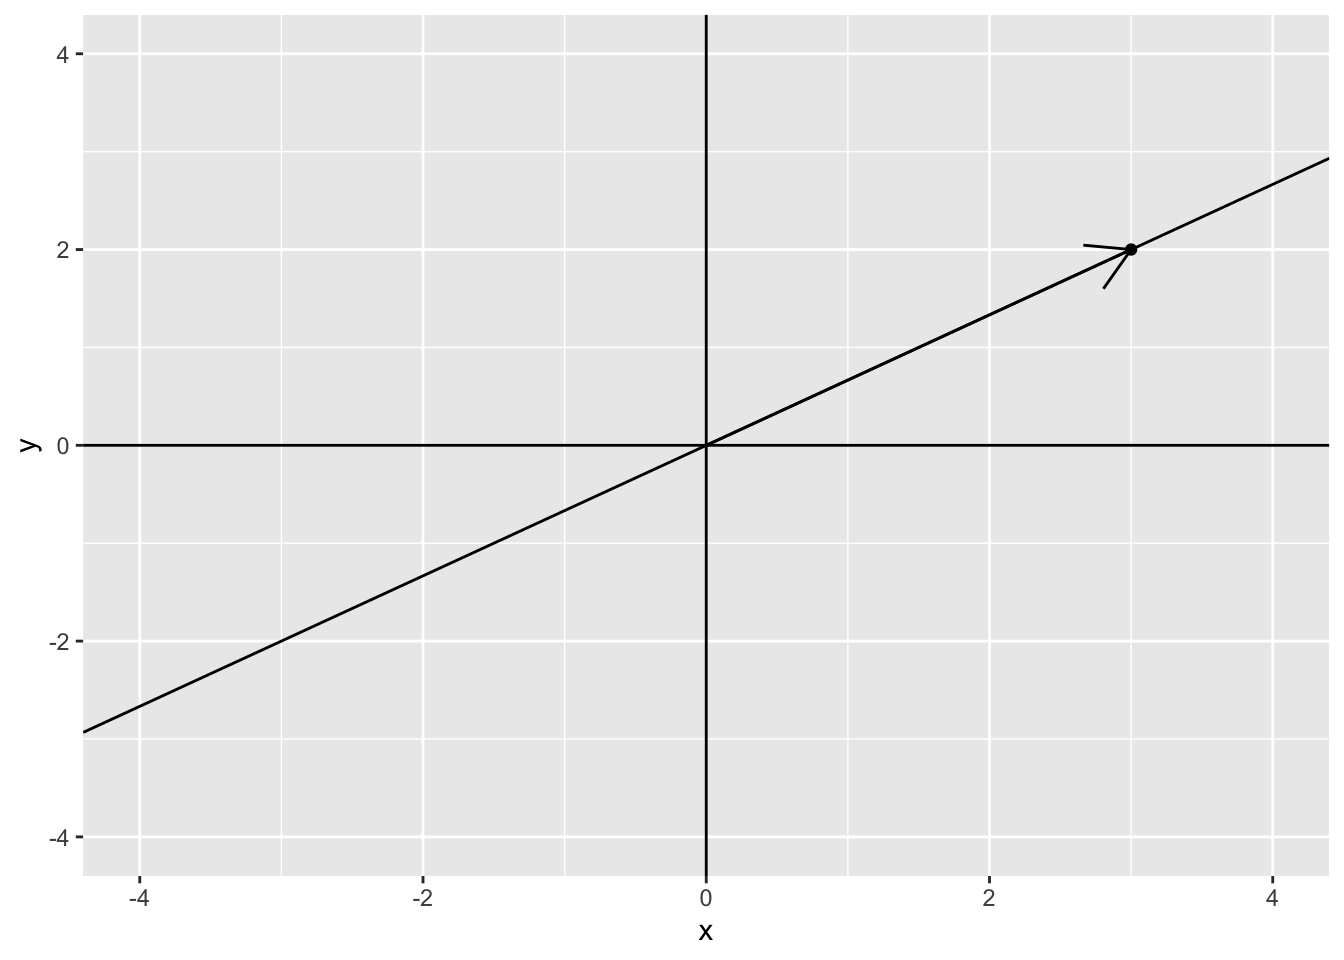
\includegraphics{multivariable-math_files/figure-latex/unnamed-chunk-57-1.pdf}

A vector space is a generalization of this representation. In \(\mathcal{R}^2\), we say that the vector \(\mathbf{z} = c(2, 3)\) is centered at the origin (0, 0) and has length 2 in the \(x\)-axis and length 3 in the \(y\)-axis. The plot below shows this vector

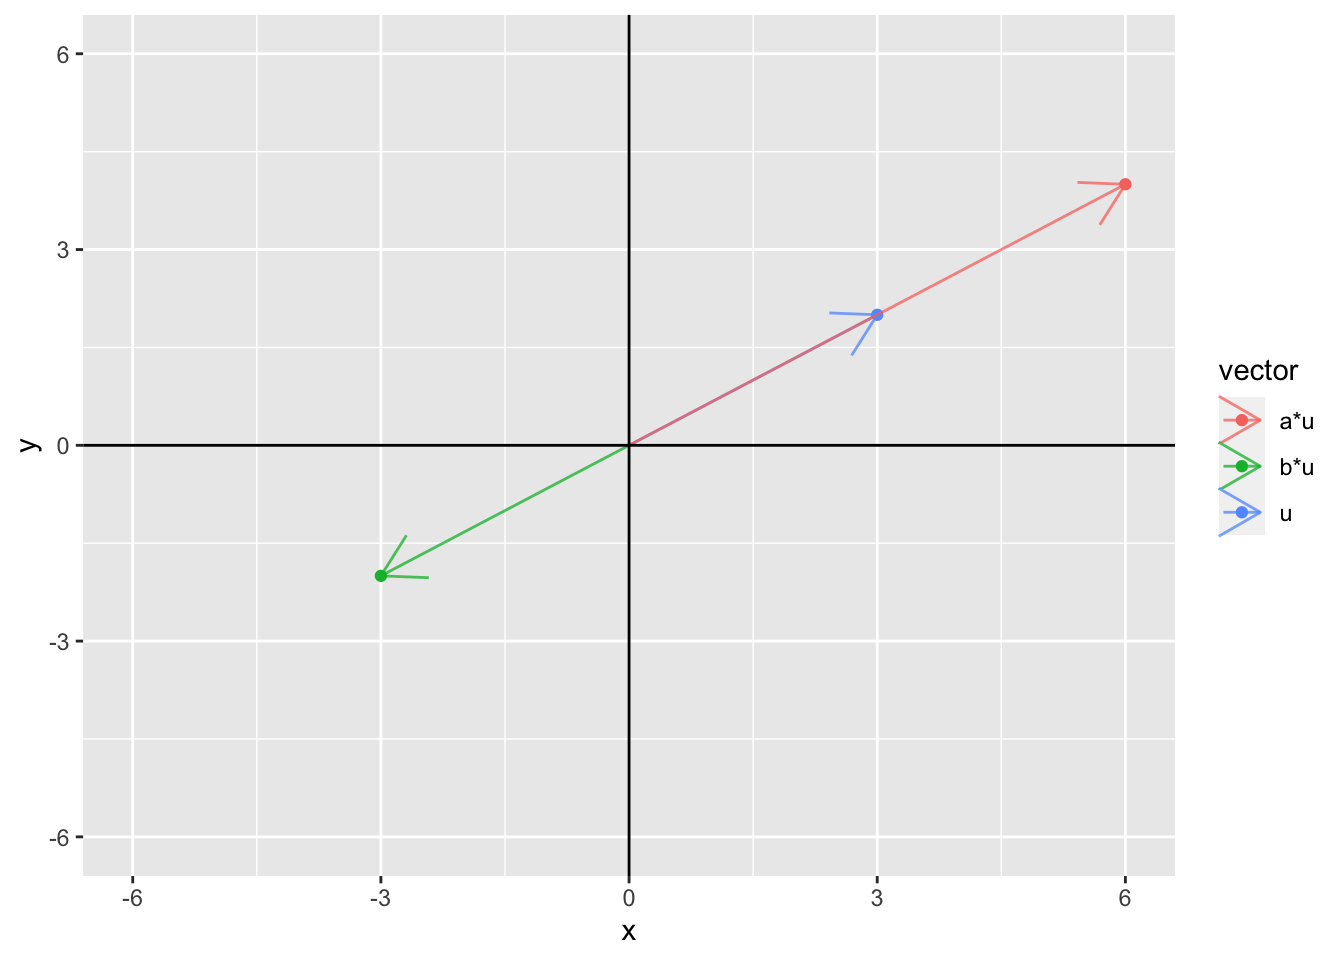
\includegraphics{multivariable-math_files/figure-latex/unnamed-chunk-58-1.pdf}

We can also decompose the vector \(\mathbf{z}\) into its \(x\) and \(y\) components. The \(x\) component of \(\mathbf{z}\) is (2, 0) and the \(y\) component of \(\mathbf{z}\) is (0, 3). The following plot shows the \(x\) component (2, 0) in blue and the \(y\) component (0, 3) in red.

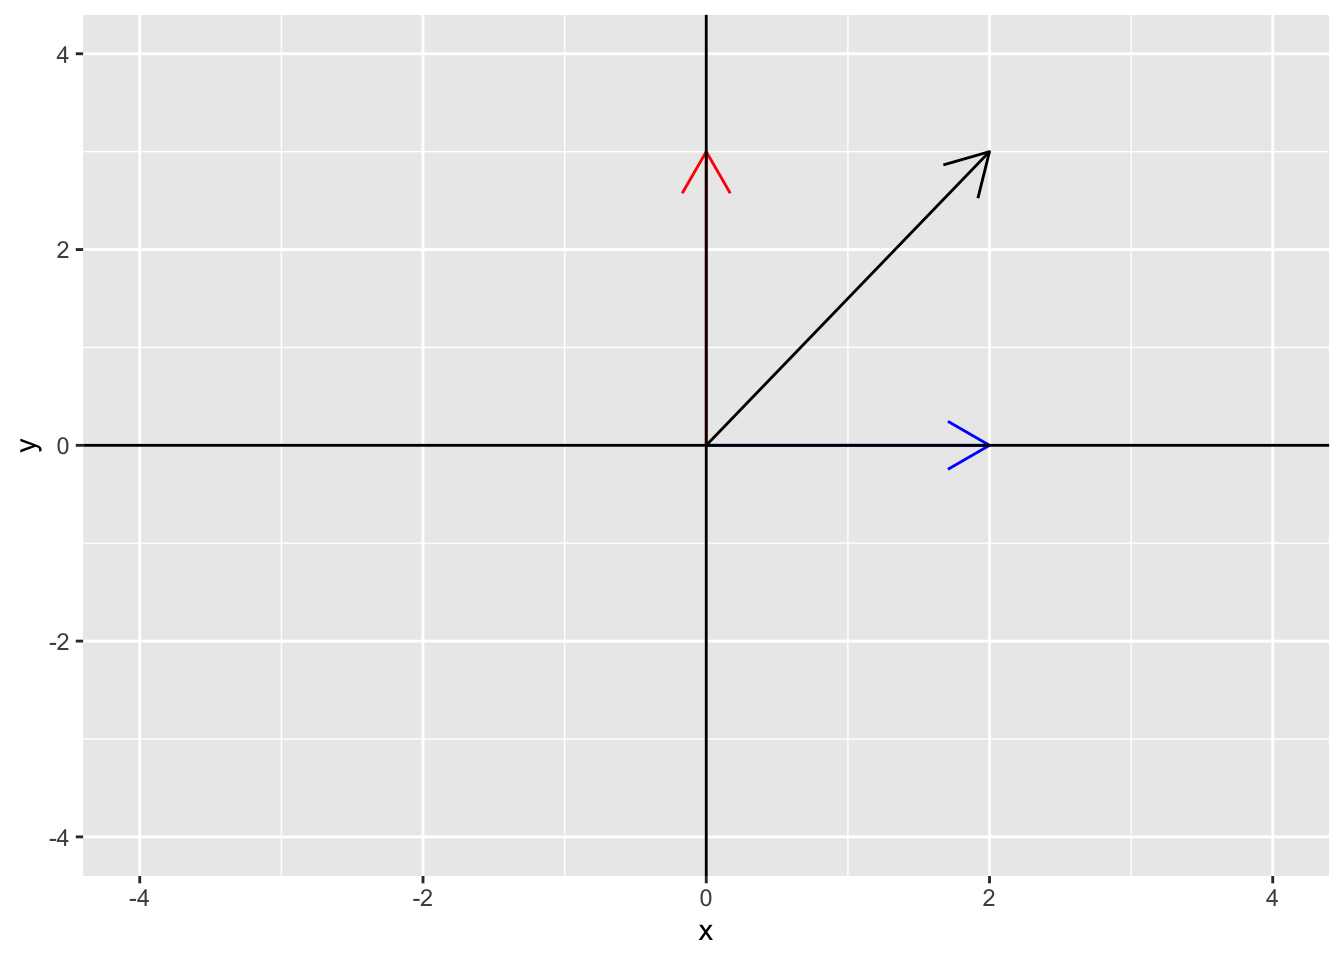
\includegraphics{multivariable-math_files/figure-latex/unnamed-chunk-59-1.pdf}

The below Shiny app allows you to plot the vector for any \((x, y)\) pair of your choosing.

The shiny app can be downloaded and run on your own computer using

\begin{Shaded}
\begin{Highlighting}[]
\KeywordTok{library}\NormalTok{(shiny)}
\KeywordTok{runGitHub}\NormalTok{(}\DataTypeTok{rep =} \StringTok{"multivariable-math"}\NormalTok{, }
          \DataTypeTok{username =} \StringTok{"jtipton25"}\NormalTok{,}
          \DataTypeTok{subdir =} \StringTok{"shiny-apps/chapter-03/vector-space"}\NormalTok{) }
\end{Highlighting}
\end{Shaded}

\hypertarget{addition-of-vectors}{%
\subsubsection{Addition of vectors}\label{addition-of-vectors}}

We can represent the addition of vectors geometrically as well. Consider the two vectors \(\mathbf{u}\) = (3, 2) and \(\mathbf{v}\) = (-2, 1) where \(\mathbf{u} + \mathbf{v}\) = (1, 3).

\begin{Shaded}
\begin{Highlighting}[]
\KeywordTok{data.frame}\NormalTok{(}\DataTypeTok{x =} \KeywordTok{c}\NormalTok{(}\DecValTok{3}\NormalTok{, }\DecValTok{-2}\NormalTok{, }\DecValTok{1}\NormalTok{), }\DataTypeTok{y =} \KeywordTok{c}\NormalTok{(}\DecValTok{2}\NormalTok{, }\DecValTok{1}\NormalTok{, }\DecValTok{3}\NormalTok{), }\DataTypeTok{vector =} \KeywordTok{c}\NormalTok{(}\StringTok{"u"}\NormalTok{, }\StringTok{"v"}\NormalTok{, }\StringTok{"u+v"}\NormalTok{)) }\OperatorTok
\StringTok{    }\KeywordTok{ggplot}\NormalTok{() }\OperatorTok{+}
\StringTok{    }\KeywordTok{geom_point}\NormalTok{(}\KeywordTok{aes}\NormalTok{(}\DataTypeTok{x =}\NormalTok{ x, }\DataTypeTok{y =}\NormalTok{ y, }\DataTypeTok{color =}\NormalTok{ vector)) }\OperatorTok{+}
\StringTok{    }\KeywordTok{geom_vline}\NormalTok{(}\DataTypeTok{xintercept =} \DecValTok{0}\NormalTok{) }\OperatorTok{+}\StringTok{ }
\StringTok{    }\KeywordTok{geom_hline}\NormalTok{(}\DataTypeTok{yintercept =} \DecValTok{0}\NormalTok{) }\OperatorTok{+}
\StringTok{    }\KeywordTok{coord_cartesian}\NormalTok{(}\DataTypeTok{xlim =} \KeywordTok{c}\NormalTok{(}\OperatorTok{-}\DecValTok{4}\NormalTok{, }\DecValTok{4}\NormalTok{), }\DataTypeTok{ylim =} \KeywordTok{c}\NormalTok{(}\OperatorTok{-}\DecValTok{4}\NormalTok{, }\DecValTok{4}\NormalTok{))}
\end{Highlighting}
\end{Shaded}

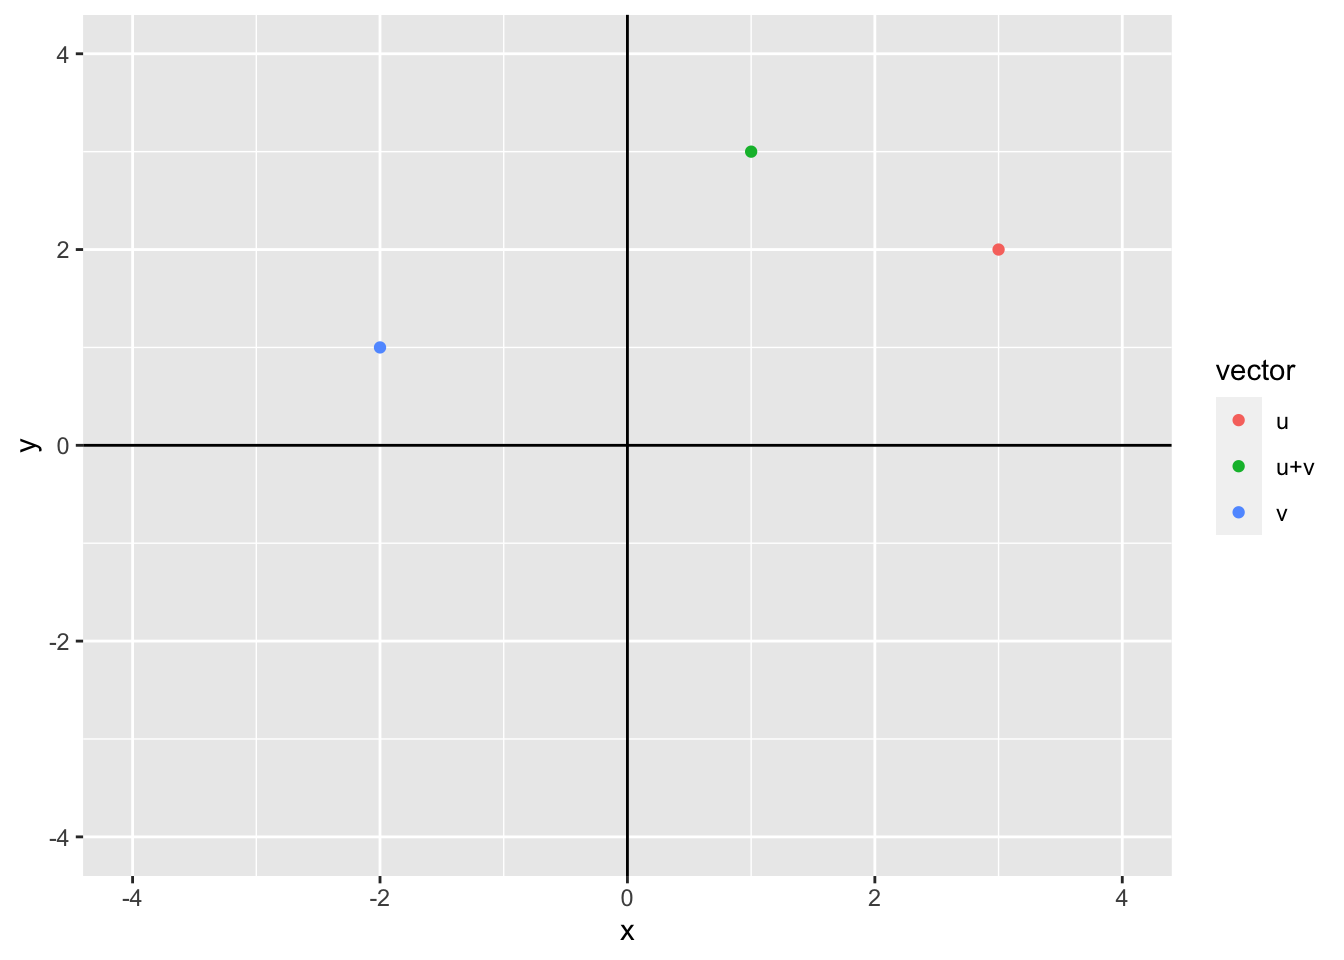
\includegraphics{multivariable-math_files/figure-latex/unnamed-chunk-62-1.pdf}

We can represent the sum using vectors by adding \(\mathbf{u}\) first then adding \(\mathbf{v}\) to \(\mathbf{u}\) or by adding \(\mathbf{v}\) first and then \(\mathbf{u}\) to get

\begin{Shaded}
\begin{Highlighting}[]
\NormalTok{df <-}\StringTok{ }\KeywordTok{data.frame}\NormalTok{(}\DataTypeTok{x =} \KeywordTok{c}\NormalTok{(}\DecValTok{0}\NormalTok{, }\DecValTok{3}\NormalTok{, }\DecValTok{1}\NormalTok{, }\DecValTok{-2}\NormalTok{), }\DataTypeTok{y =} \KeywordTok{c}\NormalTok{(}\DecValTok{0}\NormalTok{, }\DecValTok{2}\NormalTok{, }\DecValTok{3}\NormalTok{, }\DecValTok{1}\NormalTok{))}
\NormalTok{p1 <-}\StringTok{ }\KeywordTok{ggplot}\NormalTok{() }\OperatorTok{+}
\StringTok{    }\KeywordTok{geom_segment}\NormalTok{(}\KeywordTok{aes}\NormalTok{(}\DataTypeTok{x =} \DecValTok{0}\NormalTok{, }\DataTypeTok{xend =} \DecValTok{3}\NormalTok{, }\DataTypeTok{y =} \DecValTok{0}\NormalTok{, }\DataTypeTok{yend =} \DecValTok{2}\NormalTok{), }\DataTypeTok{arrow =} \KeywordTok{arrow}\NormalTok{(), }\DataTypeTok{color =} \StringTok{"blue"}\NormalTok{) }\OperatorTok{+}
\StringTok{    }\KeywordTok{geom_segment}\NormalTok{(}\KeywordTok{aes}\NormalTok{(}\DataTypeTok{x =} \DecValTok{3}\NormalTok{, }\DataTypeTok{xend =} \DecValTok{3} \OperatorTok{-}\StringTok{ }\DecValTok{2}\NormalTok{, }\DataTypeTok{y =} \DecValTok{2}\NormalTok{, }\DataTypeTok{yend =} \DecValTok{2} \OperatorTok{+}\StringTok{ }\DecValTok{1}\NormalTok{), }\DataTypeTok{arrow =} \KeywordTok{arrow}\NormalTok{(), }\DataTypeTok{color =} \StringTok{"red"}\NormalTok{) }\OperatorTok{+}
\StringTok{    }\KeywordTok{geom_segment}\NormalTok{(}\KeywordTok{aes}\NormalTok{(}\DataTypeTok{x =} \DecValTok{0}\NormalTok{, }\DataTypeTok{xend =} \DecValTok{3} \OperatorTok{-}\StringTok{ }\DecValTok{2}\NormalTok{, }\DataTypeTok{y =} \DecValTok{0}\NormalTok{, }\DataTypeTok{yend =} \DecValTok{2} \OperatorTok{+}\StringTok{ }\DecValTok{1}\NormalTok{), }\DataTypeTok{arrow =} \KeywordTok{arrow}\NormalTok{(), }\DataTypeTok{color =} \StringTok{"black"}\NormalTok{) }\OperatorTok{+}
\StringTok{    }\KeywordTok{geom_vline}\NormalTok{(}\DataTypeTok{xintercept =} \DecValTok{0}\NormalTok{) }\OperatorTok{+}\StringTok{ }
\StringTok{    }\KeywordTok{geom_hline}\NormalTok{(}\DataTypeTok{yintercept =} \DecValTok{0}\NormalTok{) }\OperatorTok{+}
\StringTok{    }\KeywordTok{coord_cartesian}\NormalTok{(}\DataTypeTok{xlim =} \KeywordTok{c}\NormalTok{(}\OperatorTok{-}\DecValTok{4}\NormalTok{, }\DecValTok{4}\NormalTok{), }\DataTypeTok{ylim =} \KeywordTok{c}\NormalTok{(}\OperatorTok{-}\DecValTok{4}\NormalTok{, }\DecValTok{4}\NormalTok{)) }\OperatorTok{+}\StringTok{ }
\StringTok{    }\KeywordTok{geom_polygon}\NormalTok{(}\DataTypeTok{data =}\NormalTok{ df, }\KeywordTok{aes}\NormalTok{(}\DataTypeTok{x =}\NormalTok{ x, }\DataTypeTok{y =}\NormalTok{ y), }\DataTypeTok{fill =} \StringTok{"grey"}\NormalTok{, }\DataTypeTok{alpha =} \FloatTok{0.5}\NormalTok{) }\OperatorTok{+}
\StringTok{    }\KeywordTok{ggtitle}\NormalTok{(}\StringTok{"u + v"}\NormalTok{)}
\NormalTok{p2 <-}\StringTok{ }\KeywordTok{ggplot}\NormalTok{() }\OperatorTok{+}
\StringTok{    }\KeywordTok{geom_segment}\NormalTok{(}\KeywordTok{aes}\NormalTok{(}\DataTypeTok{x =} \DecValTok{0}\NormalTok{, }\DataTypeTok{xend =} \DecValTok{-2}\NormalTok{, }\DataTypeTok{y =} \DecValTok{0}\NormalTok{, }\DataTypeTok{yend =} \DecValTok{1}\NormalTok{), }\DataTypeTok{arrow =} \KeywordTok{arrow}\NormalTok{(), }\DataTypeTok{color =} \StringTok{"red"}\NormalTok{) }\OperatorTok{+}
\StringTok{    }\KeywordTok{geom_segment}\NormalTok{(}\KeywordTok{aes}\NormalTok{(}\DataTypeTok{x =} \DecValTok{-2}\NormalTok{, }\DataTypeTok{xend =} \DecValTok{-2} \OperatorTok{+}\StringTok{ }\DecValTok{3}\NormalTok{, }\DataTypeTok{y =} \DecValTok{1}\NormalTok{, }\DataTypeTok{yend =} \DecValTok{1} \OperatorTok{+}\StringTok{ }\DecValTok{2}\NormalTok{), }\DataTypeTok{arrow =} \KeywordTok{arrow}\NormalTok{(), }\DataTypeTok{color =} \StringTok{"blue"}\NormalTok{) }\OperatorTok{+}
\StringTok{    }\KeywordTok{geom_segment}\NormalTok{(}\KeywordTok{aes}\NormalTok{(}\DataTypeTok{x =} \DecValTok{0}\NormalTok{, }\DataTypeTok{xend =} \DecValTok{3} \OperatorTok{-}\StringTok{ }\DecValTok{2}\NormalTok{, }\DataTypeTok{y =} \DecValTok{0}\NormalTok{, }\DataTypeTok{yend =} \DecValTok{2} \OperatorTok{+}\StringTok{ }\DecValTok{1}\NormalTok{), }\DataTypeTok{arrow =} \KeywordTok{arrow}\NormalTok{(), }\DataTypeTok{color =} \StringTok{"black"}\NormalTok{) }\OperatorTok{+}
\StringTok{    }\KeywordTok{geom_vline}\NormalTok{(}\DataTypeTok{xintercept =} \DecValTok{0}\NormalTok{) }\OperatorTok{+}\StringTok{ }
\StringTok{    }\KeywordTok{geom_hline}\NormalTok{(}\DataTypeTok{yintercept =} \DecValTok{0}\NormalTok{) }\OperatorTok{+}
\StringTok{    }\KeywordTok{coord_cartesian}\NormalTok{(}\DataTypeTok{xlim =} \KeywordTok{c}\NormalTok{(}\OperatorTok{-}\DecValTok{4}\NormalTok{, }\DecValTok{4}\NormalTok{), }\DataTypeTok{ylim =} \KeywordTok{c}\NormalTok{(}\OperatorTok{-}\DecValTok{4}\NormalTok{, }\DecValTok{4}\NormalTok{)) }\OperatorTok{+}
\StringTok{    }\KeywordTok{geom_polygon}\NormalTok{(}\DataTypeTok{data =}\NormalTok{ df, }\KeywordTok{aes}\NormalTok{(}\DataTypeTok{x =}\NormalTok{ x, }\DataTypeTok{y =}\NormalTok{ y), }\DataTypeTok{fill =} \StringTok{"grey"}\NormalTok{, }\DataTypeTok{alpha =} \FloatTok{0.5}\NormalTok{) }\OperatorTok{+}
\StringTok{    }\KeywordTok{ggtitle}\NormalTok{(}\StringTok{"v + u"}\NormalTok{)}
\NormalTok{p1 }\OperatorTok{+}\StringTok{ }\NormalTok{p2}
\end{Highlighting}
\end{Shaded}

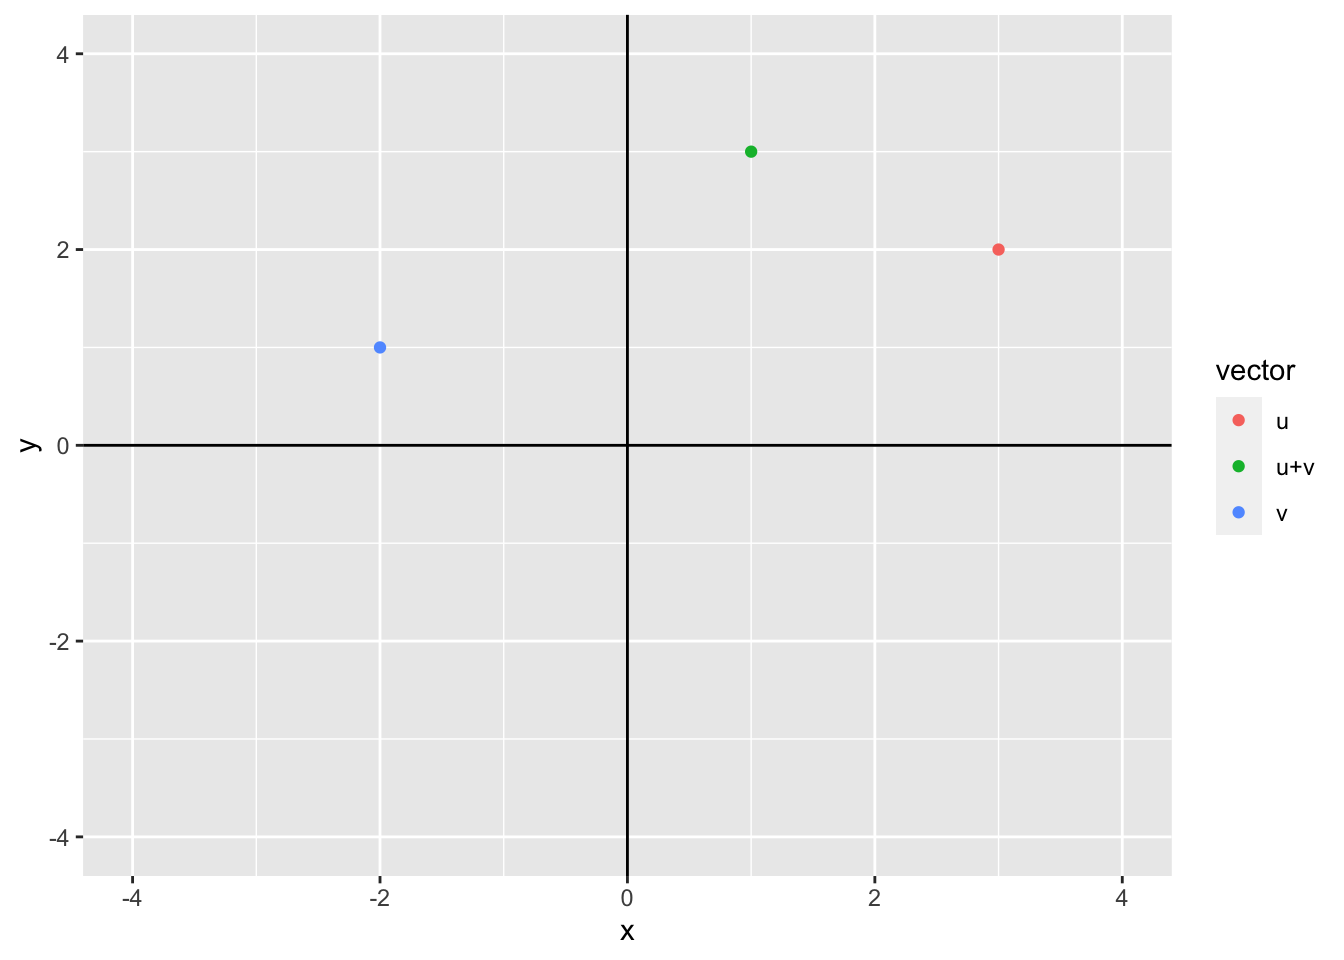
\includegraphics{multivariable-math_files/figure-latex/unnamed-chunk-63-1.pdf}

Notice that the sum of these vectors defines a parallelogram where the sum \(\mathbf{u} + \mathbf{v}\) is the diagonal of the shaded parallelogram. This geometric interpretation will serve as a basis for interpreting vector equations in higher dimensions where typical visualization methods fail.

\hypertarget{scalar-multiplication-of-vectors}{%
\subsection{Scalar multiplication of vectors}\label{scalar-multiplication-of-vectors}}

We can represent the multiplication of a vector by a scalar geometrically as well. Consider the vector \(\mathbf{u}\) = (3, 2) and the scalars \(a = 2\) and \(b = -1\). Then, we can plot \(\mathbf{u}\), \(a\mathbf{u}\), and \(b\mathbf{u}\).

\begin{Shaded}
\begin{Highlighting}[]
\KeywordTok{data.frame}\NormalTok{(}\DataTypeTok{x =} \KeywordTok{c}\NormalTok{(}\DecValTok{3}\NormalTok{, }\DecValTok{2} \OperatorTok{*}\StringTok{ }\DecValTok{3}\NormalTok{, }\DecValTok{-1} \OperatorTok{*}\StringTok{ }\DecValTok{3}\NormalTok{), }\DataTypeTok{y =} \KeywordTok{c}\NormalTok{(}\DecValTok{2}\NormalTok{, }\DecValTok{2} \OperatorTok{*}\StringTok{ }\DecValTok{2}\NormalTok{, }\DecValTok{-1} \OperatorTok{*}\StringTok{ }\DecValTok{2}\NormalTok{), }\DataTypeTok{vector =} \KeywordTok{c}\NormalTok{(}\StringTok{"u"}\NormalTok{, }\StringTok{"a*u"}\NormalTok{, }\StringTok{"b*u"}\NormalTok{)) }\OperatorTok
\StringTok{    }\KeywordTok{ggplot}\NormalTok{() }\OperatorTok{+}
\StringTok{    }\KeywordTok{geom_point}\NormalTok{(}\KeywordTok{aes}\NormalTok{(}\DataTypeTok{x =}\NormalTok{ x, }\DataTypeTok{y =}\NormalTok{ y, }\DataTypeTok{color =}\NormalTok{ vector)) }\OperatorTok{+}
\StringTok{    }\KeywordTok{geom_segment}\NormalTok{(}\KeywordTok{aes}\NormalTok{(}\DataTypeTok{x =} \DecValTok{0}\NormalTok{, }\DataTypeTok{xend =}\NormalTok{ x, }\DataTypeTok{y =} \DecValTok{0}\NormalTok{, }\DataTypeTok{yend =}\NormalTok{ y, }\DataTypeTok{color =}\NormalTok{ vector), }\DataTypeTok{arrow =} \KeywordTok{arrow}\NormalTok{(), }\DataTypeTok{alpha =} \FloatTok{0.75}\NormalTok{) }\OperatorTok{+}
\StringTok{    }\KeywordTok{geom_vline}\NormalTok{(}\DataTypeTok{xintercept =} \DecValTok{0}\NormalTok{) }\OperatorTok{+}\StringTok{ }
\StringTok{    }\KeywordTok{geom_hline}\NormalTok{(}\DataTypeTok{yintercept =} \DecValTok{0}\NormalTok{) }\OperatorTok{+}
\StringTok{    }\KeywordTok{coord_cartesian}\NormalTok{(}\DataTypeTok{xlim =} \KeywordTok{c}\NormalTok{(}\OperatorTok{-}\DecValTok{6}\NormalTok{, }\DecValTok{6}\NormalTok{), }\DataTypeTok{ylim =} \KeywordTok{c}\NormalTok{(}\OperatorTok{-}\DecValTok{6}\NormalTok{, }\DecValTok{6}\NormalTok{))}
\end{Highlighting}
\end{Shaded}

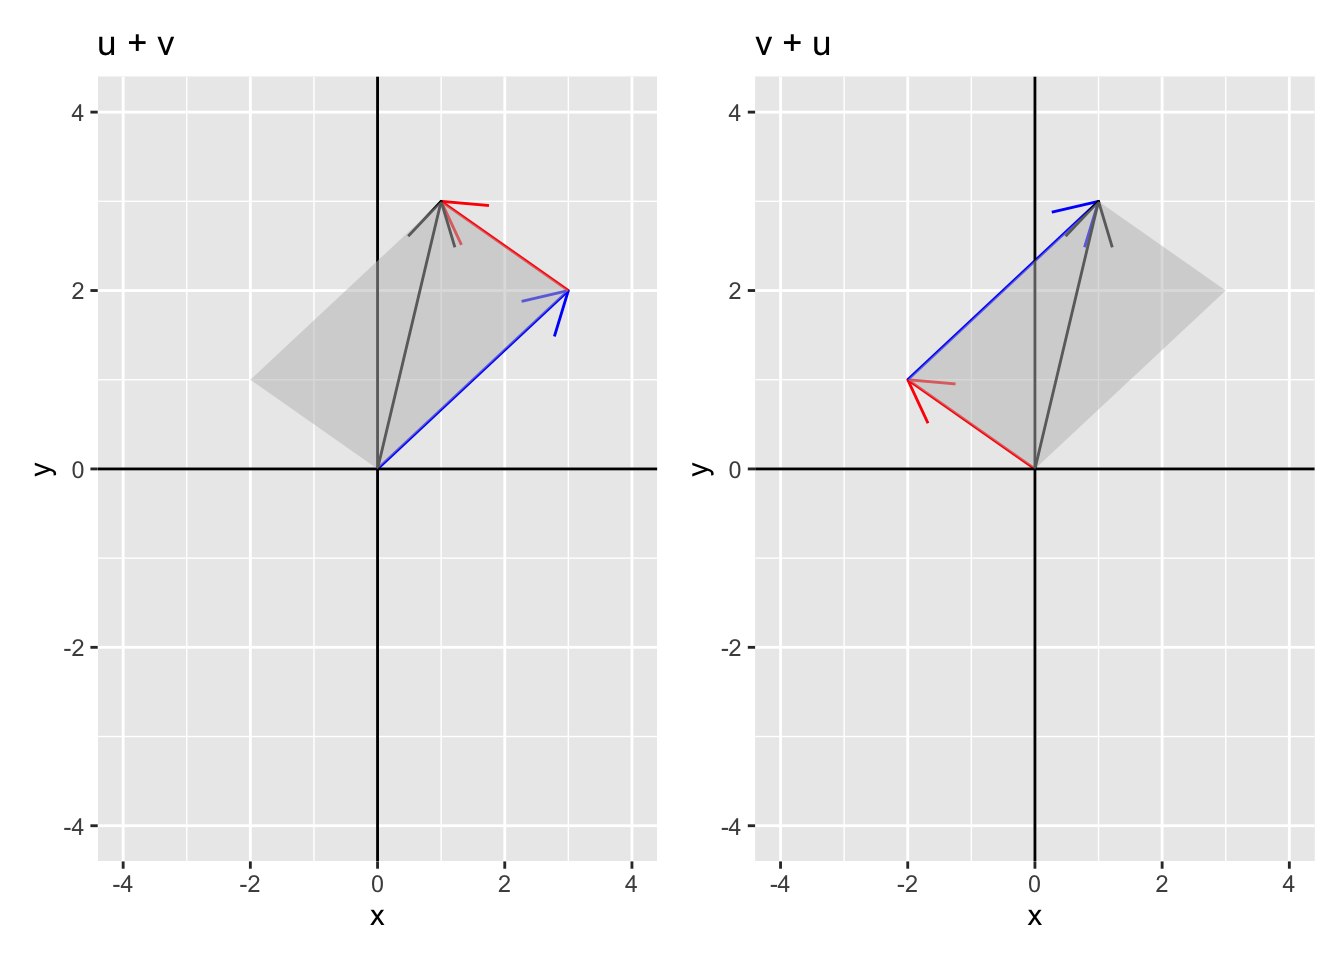
\includegraphics{multivariable-math_files/figure-latex/unnamed-chunk-64-1.pdf}

In fact, if \(a\) is allowed to take on any values, then the set of all possible values of \(a \mathbf{u}\) for all values of \(a\) defines an infinite line

\begin{Shaded}
\begin{Highlighting}[]
\KeywordTok{ggplot}\NormalTok{() }\OperatorTok{+}
\StringTok{    }\KeywordTok{geom_abline}\NormalTok{(}\DataTypeTok{slope =} \DecValTok{2}\OperatorTok{/}\DecValTok{3}\NormalTok{, }\DataTypeTok{intercept =} \DecValTok{0}\NormalTok{) }\OperatorTok{+}\StringTok{  }
\StringTok{    }\KeywordTok{geom_point}\NormalTok{(}\KeywordTok{aes}\NormalTok{(}\DataTypeTok{x =} \DecValTok{3}\NormalTok{, }\DataTypeTok{y =} \DecValTok{2}\NormalTok{)) }\OperatorTok{+}
\StringTok{    }\KeywordTok{geom_segment}\NormalTok{(}\KeywordTok{aes}\NormalTok{(}\DataTypeTok{x =} \DecValTok{0}\NormalTok{, }\DataTypeTok{xend =} \DecValTok{3}\NormalTok{, }\DataTypeTok{y =} \DecValTok{0}\NormalTok{, }\DataTypeTok{yend =} \DecValTok{2}\NormalTok{), }\DataTypeTok{arrow =} \KeywordTok{arrow}\NormalTok{(), }\DataTypeTok{color =} \StringTok{"black"}\NormalTok{) }\OperatorTok{+}
\StringTok{    }\KeywordTok{geom_vline}\NormalTok{(}\DataTypeTok{xintercept =} \DecValTok{0}\NormalTok{) }\OperatorTok{+}\StringTok{ }
\StringTok{    }\KeywordTok{geom_hline}\NormalTok{(}\DataTypeTok{yintercept =} \DecValTok{0}\NormalTok{) }\OperatorTok{+}
\StringTok{    }\KeywordTok{coord_cartesian}\NormalTok{(}\DataTypeTok{xlim =} \KeywordTok{c}\NormalTok{(}\OperatorTok{-}\DecValTok{4}\NormalTok{, }\DecValTok{4}\NormalTok{), }\DataTypeTok{ylim =} \KeywordTok{c}\NormalTok{(}\OperatorTok{-}\DecValTok{4}\NormalTok{, }\DecValTok{4}\NormalTok{)) }
\end{Highlighting}
\end{Shaded}

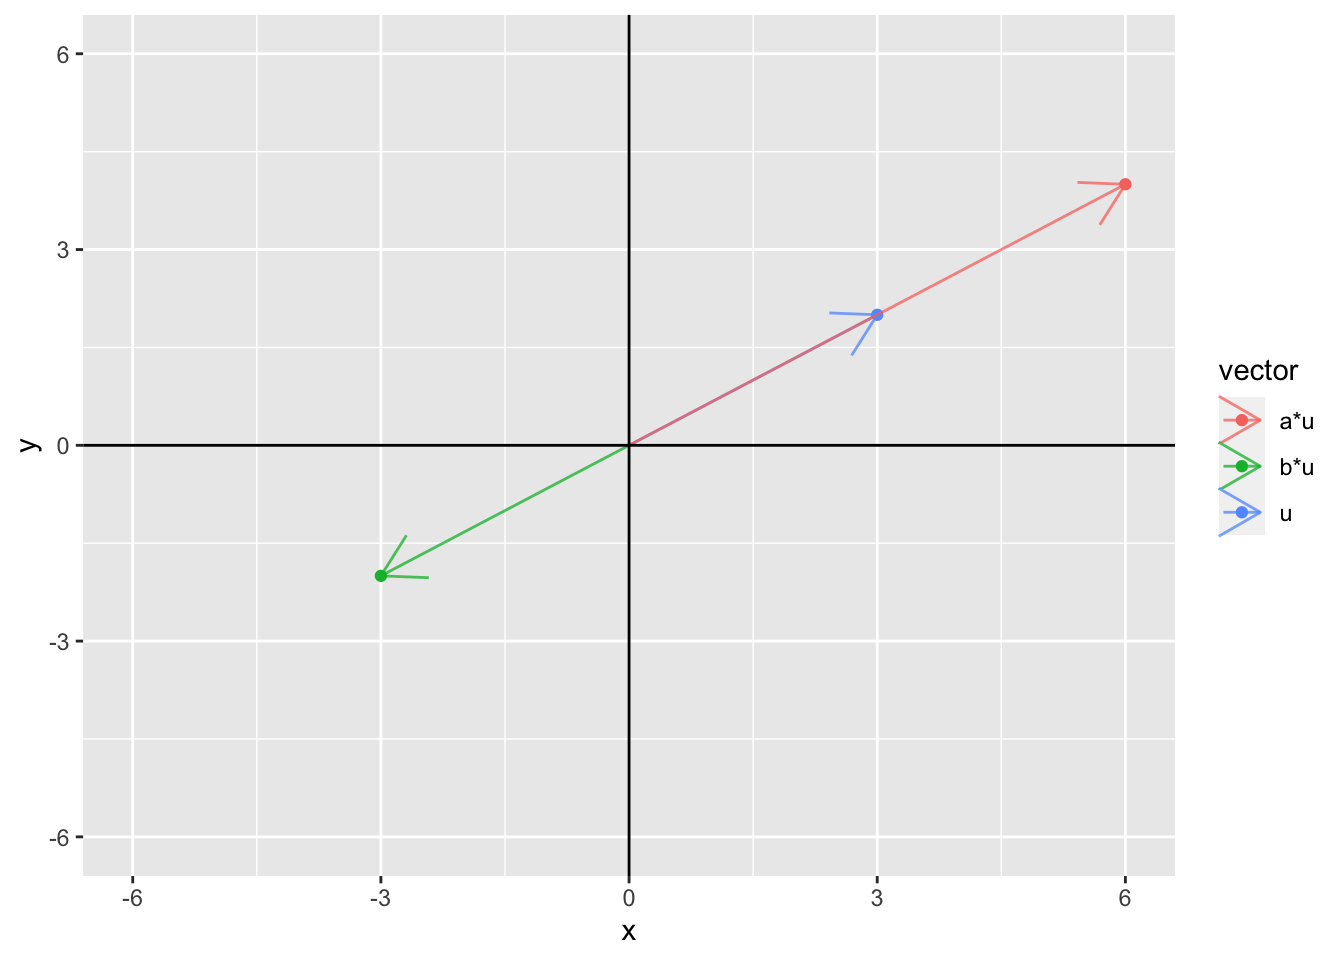
\includegraphics{multivariable-math_files/figure-latex/unnamed-chunk-65-1.pdf}

\hypertarget{the-geometric-interpretation-of-vectors-in-mathcalr3}{%
\subsection{\texorpdfstring{The geometric interpretation of vectors in \(\mathcal{R}^3\)}{The geometric interpretation of vectors in \textbackslash mathcal\{R\}\^{}3}}\label{the-geometric-interpretation-of-vectors-in-mathcalr3}}

Let the vector \(\mathbf{u} = c(-2, 3, 5)\). Then, the figure below shows the vector in 3 dimensions.

\textbf{Draw picture by hand}

\hypertarget{the-geometric-interpretation-of-vectors-in-mathcalrn}{%
\subsection{\texorpdfstring{The geometric interpretation of vectors in \(\mathcal{R}^n\)}{The geometric interpretation of vectors in \textbackslash mathcal\{R\}\^{}n}}\label{the-geometric-interpretation-of-vectors-in-mathcalrn}}

As the number of dimensions increases, the same interpretation can be used, but the ability to visualize higher dimensions becomes more difficult.

\hypertarget{linear-combinations-of-vectors}{%
\subsection{Linear Combinations of Vectors}\label{linear-combinations-of-vectors}}

We say that for any two scalars \(a\) and \(b\) and any two vectors \(\mathbf{x}\) and \(\mathbf{y}\) of length \(n\), the sum

\[
\begin{aligned}
a \mathbf{x} + b \mathbf{y} & = \begin{pmatrix}
a x_1 + b y_1 \\
a x_2 + b y_2 \\
\vdots \\
a x_n + b y_n \\
\end{pmatrix}
\end{aligned}
\]

is called a linear combination. The idea of a linear combination can be extended to \(K\) different scalars \(\{ a_1, \ldots, a_K \}\) and \(K\) different vectors \(\{ \mathbf{x}_1, \ldots, \mathbf{x}_K\}\) each of length \(n\) as

\[
 \begin{aligned}
a_1 \mathbf{x}_1 + a_2 \mathbf{x}_2 +  \ldots + a_K \mathbf{x}_K = 
\sum_{k=1}^K a_k \mathbf{x}_k & = \begin{pmatrix}
\sum_{k=1}^K a_k x_{k1} \\
\sum_{k=1}^K a_k x_{k2} \\
\vdots \\
\sum_{k=1}^K a_k x_{kn} \\
\end{pmatrix}
\end{aligned}
\]
The scalars \(a_k\) are called \textbf{coefficients} (sometimes also called \textbf{weights}).

\begin{itemize}
\tightlist
\item
  \textbf{Example:} Consider the linear combination \(a \mathbf{u} + b \mathbf{v}\) where
\end{itemize}

\[
\begin{aligned}
\mathbf{u} = \begin{pmatrix} 3 \\ 6\end{pmatrix} && \mathbf{v} = \begin{pmatrix} -2 \\ 1\end{pmatrix}. \end{aligned}
\]
Are there values of \(a\) and \(b\) such \(a \mathbf{u} + b \mathbf{v} = \begin{pmatrix} 9 \\ - 4 \end{pmatrix}\)? To answer this question, we can write the linear combination as
\[
\begin{aligned}
a \begin{pmatrix} 3 \\ 6\end{pmatrix} + b \begin{pmatrix} -2 \\ 1\end{pmatrix} & = \begin{pmatrix} 9 \\ -4 \end{pmatrix} 
\end{aligned}
\]
which can be written using the property of scalar multiplication as
\[
\begin{aligned}
\begin{pmatrix} 3a \\ 6a \end{pmatrix} + \begin{pmatrix} -2b \\ b \end{pmatrix} & = \begin{pmatrix} 9 \\ -4 \end{pmatrix}
\end{aligned}
\]
and using properties of vector addition can be written as
\[
\begin{aligned}
\begin{pmatrix} 3a - 2b \\ 6a + b \end{pmatrix} & = \begin{pmatrix} 9 \\ -4 \end{pmatrix}
\end{aligned}
\]
Recognizing this as a system of linear equations
\[
\begin{aligned}
3a - 2b & = 9 \\ 
6a + b & = -4,
\end{aligned}
\]
the system of equations can be written in an augmented matrix form as
\[
\begin{aligned}
\begin{pmatrix}
3  & - 2 & 9\\
6  &   1 & -4 
\end{pmatrix}
\end{aligned}
\]
Reducing the augmented matrix to reduced row echelon form gives

\begin{Shaded}
\begin{Highlighting}[]
\KeywordTok{rref}\NormalTok{(}\KeywordTok{matrix}\NormalTok{(}\KeywordTok{c}\NormalTok{(}\DecValTok{3}\NormalTok{, }\DecValTok{6}\NormalTok{, }\DecValTok{-2}\NormalTok{, }\DecValTok{1}\NormalTok{, }\DecValTok{9}\NormalTok{, }\DecValTok{-4}\NormalTok{), }\DecValTok{2}\NormalTok{, }\DecValTok{3}\NormalTok{))}
\end{Highlighting}
\end{Shaded}

\begin{verbatim}
##      [,1] [,2]        [,3]
## [1,]    1    0  0.06666667
## [2,]    0    1 -4.40000000
\end{verbatim}

which has solutions \(a = 0.0667\) and \(b = -4.4\).

\begin{itemize}
\tightlist
\item
  \textbf{Result:} Any vector equation \(a_1 \mathbf{x}_1 + a_2 \mathbf{x}_2 + \ldots + a_K \mathbf{x}_K = \mathbf{c}\) for a given constant vector \(\mathbf{b}\) has the same solution set as the augmented matrix
\end{itemize}

\[
\begin{aligned}
\begin{pmatrix} \mathbf{x}_1 & \mathbf{x}_2 & \cdots & \mathbf{x}_K & \mathbf{b} \end{pmatrix}
\end{aligned}
\]
Equivalently, the set of vectors \(\{\mathbf{x}_k\}_{k=1}^K\) can only be combined with linear coefficients \(\{a_k\}_{k=1}^K\) to equal the vector \(\mathbf{b}\) if the linear system of equations is consistent.

\hypertarget{the-geometric-interpretation-of-linear-combinations-of-vectors}{%
\subsection{The geometric interpretation of linear combinations of vectors}\label{the-geometric-interpretation-of-linear-combinations-of-vectors}}

Consider the vectors \(\mathbf{u} = \begin{pmatrix} \sqrt{2} \\ - \sqrt{2} \end{pmatrix}\) and \(\mathbf{v} = \begin{pmatrix} 1 \\ 1 \end{pmatrix}\) shown in the figure below on the left.

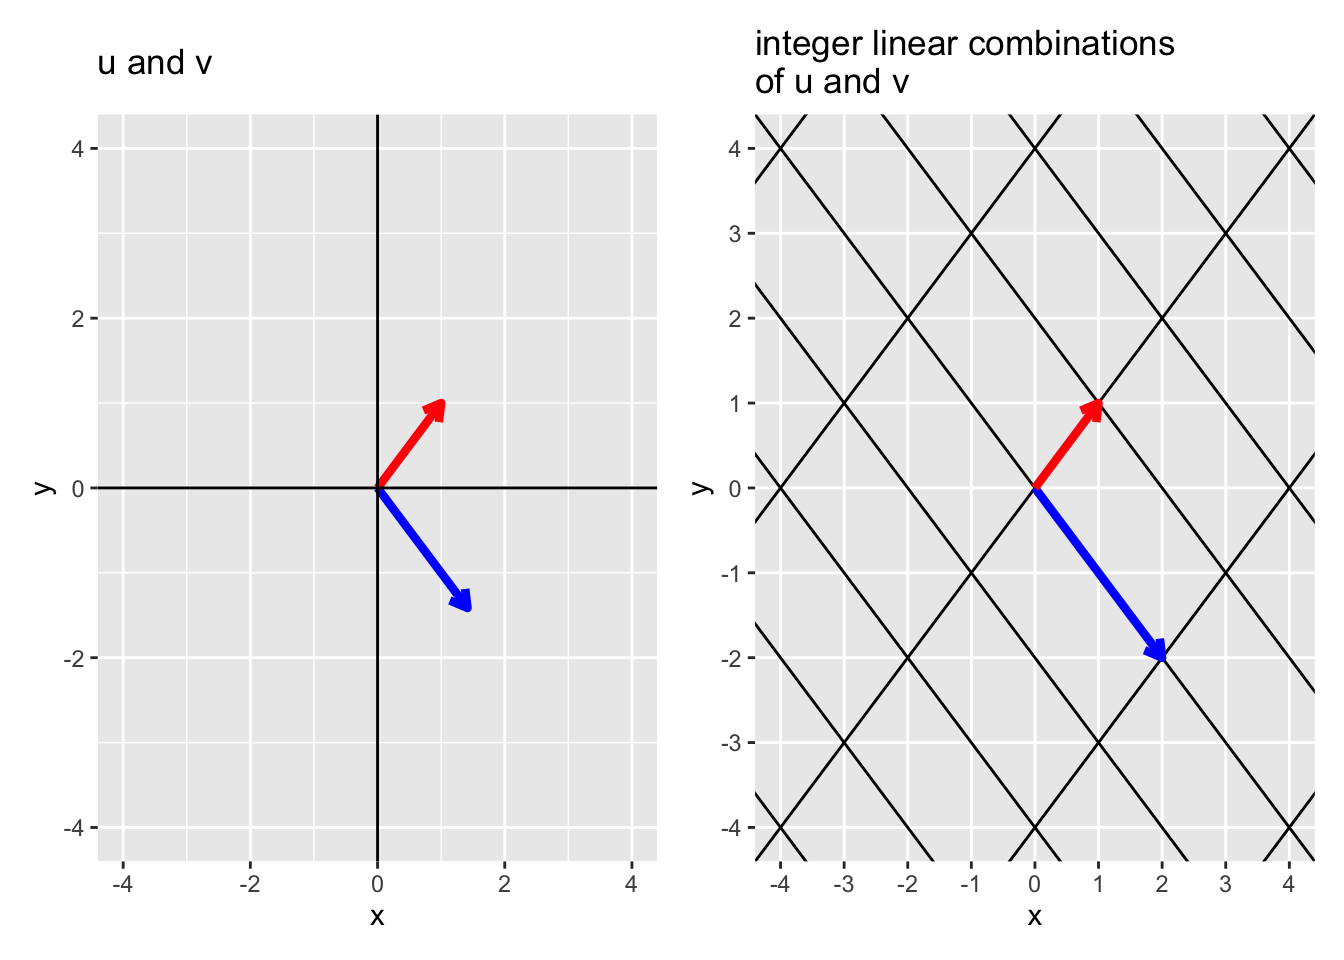
\includegraphics{multivariable-math_files/figure-latex/unnamed-chunk-68-1.pdf}

\begin{itemize}
\tightlist
\item
  \textbf{Exercise:} Given \(\mathbf{u} = \begin{pmatrix} 3 \\ -1 \end{pmatrix}\) and \(\mathbf{v} = \begin{pmatrix} 0 \\ 1 \end{pmatrix}\), estimate the linear combination of \(\mathbf{u}\) and \(\mathbf{v}\) that gives the point \(\mathbf{w}\) in the figure below.
\end{itemize}

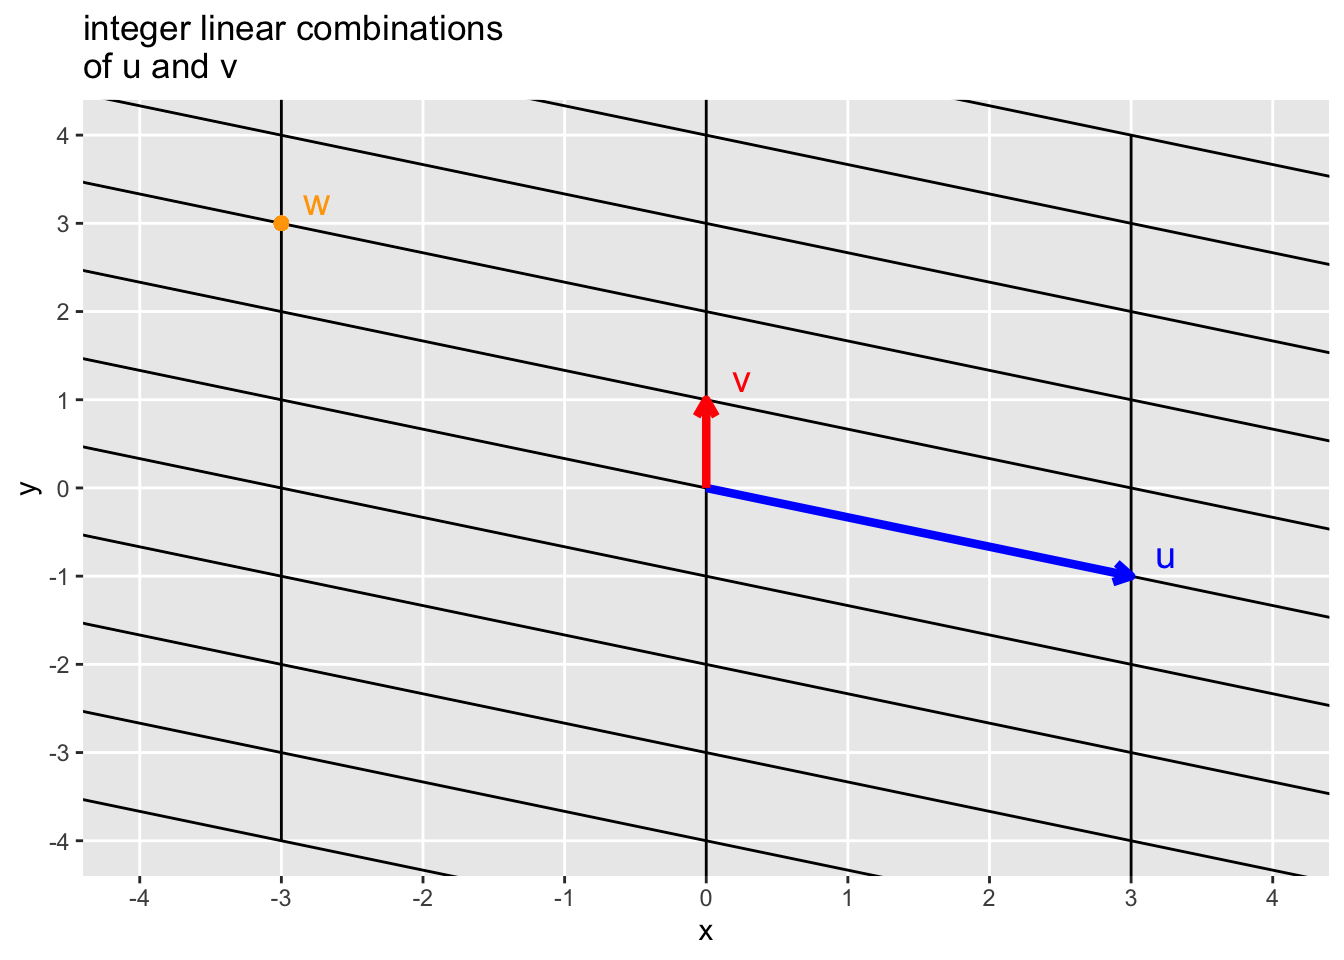
\includegraphics{multivariable-math_files/figure-latex/unnamed-chunk-69-1.pdf}

\hypertarget{span}{%
\section{Span}\label{span}}

\begin{definition}[Span]
\protect\hypertarget{def:span}{}\label{def:span}Let \(\mathbf{a}_1, \ldots, \mathbf{a}_K\) be vectors in \(\mathcal{R}^n\). We say the vector \(\mathbf{w}\) is in the span of \(\mathbf{a}_1, \ldots, \mathbf{a}_K\) (\(\mathbf{w} \in \mbox{span}\{ \mathbf{a}_1, \ldots, \mathbf{a}_K \}\)) if there exists coefficients \(x_1, \ldots, x_K\) such that \(\mathbf{w} = \sum_{k=1}^K x_k \mathbf{a}_k\).
\end{definition}

\begin{example}
While not a vector notation, you already understand the span from polynomial functions. For example, assume you have the functions 1, \(x\), and \(x^2\). Then, the functions \(-4 + 3x^2\) (\(a_1 = -4, a_2 = 0, a_3 = 3\)) and \(-3 + 4x - 2x^2\) (\(a_1 = -3, a_2 = 4, a_3 = -2\)) are in the span of functions \(\{1, x, x^2\}\), but the functions \(x^3\), \(x^4 - 2x^2\), etc., are not in the span of \(\{1, x, x^2\}\) because you cannot write these as a linear combination of \(a_1 1 + a_2 x + a_3 x^2\).
\end{example}

\hypertarget{geometric-example-of-the-span}{%
\subsection{Geometric example of the span}\label{geometric-example-of-the-span}}

\begin{itemize}
\tightlist
\item
  \textbf{Example:} Consider the vector \(\mathbf{u} = \begin{pmatrix} 2 \\ 1 \end{pmatrix}\). Then, the vector \(\mathbf{w} = \begin{pmatrix} 4 \\ 2 \end{pmatrix}\) is in the \(\mbox{span}\{\mathbf{u}\}\) because \(\mathbf{w} = 2 \mathbf{u}\) but the vector \(\mathbf{v} = \begin{pmatrix} 4 \\ -4 \end{pmatrix}\) is not in the \(\mbox{span}\{\mathbf{u}\}\) because there is no coefficient \(a\) such that \(\mathbf{w} = a \mathbf{u}\). In this example, the vector \(\mathbf{u}\) is a 2-dimensional vector (lives in \(\mathcal{R}^2\)--a plane) but the \(\mbox{span}\{\mathbf{u}\}\) lives in 1-dimension (a line).
\end{itemize}

\begin{Shaded}
\begin{Highlighting}[]
\KeywordTok{ggplot}\NormalTok{() }\OperatorTok{+}
\StringTok{    }\KeywordTok{geom_abline}\NormalTok{(}\DataTypeTok{slope =} \DecValTok{1}\OperatorTok{/}\DecValTok{2}\NormalTok{, }\DataTypeTok{intercept =} \DecValTok{0}\NormalTok{, }\DataTypeTok{color =} \StringTok{"blue"}\NormalTok{, }\DataTypeTok{size =} \DecValTok{2}\NormalTok{) }\OperatorTok{+}\StringTok{  }
\StringTok{    }\KeywordTok{geom_segment}\NormalTok{(}\KeywordTok{aes}\NormalTok{(}\DataTypeTok{x =} \DecValTok{0}\NormalTok{, }\DataTypeTok{xend =} \DecValTok{2}\NormalTok{, }\DataTypeTok{y =} \DecValTok{0}\NormalTok{, }\DataTypeTok{yend =} \DecValTok{1}\NormalTok{), }\DataTypeTok{arrow =} \KeywordTok{arrow}\NormalTok{(}\DataTypeTok{length =} \KeywordTok{unit}\NormalTok{(}\FloatTok{0.1}\NormalTok{, }\StringTok{"inches"}\NormalTok{)), }\DataTypeTok{size =} \FloatTok{1.5}\NormalTok{, }\DataTypeTok{color =} \StringTok{"red"}\NormalTok{) }\OperatorTok{+}
\StringTok{    }\KeywordTok{geom_segment}\NormalTok{(}\KeywordTok{aes}\NormalTok{(}\DataTypeTok{x =} \DecValTok{0}\NormalTok{, }\DataTypeTok{xend =} \DecValTok{4}\NormalTok{, }\DataTypeTok{y =} \DecValTok{0}\NormalTok{, }\DataTypeTok{yend =} \DecValTok{2}\NormalTok{), }\DataTypeTok{arrow =} \KeywordTok{arrow}\NormalTok{(}\DataTypeTok{length =} \KeywordTok{unit}\NormalTok{(}\FloatTok{0.1}\NormalTok{, }\StringTok{"inches"}\NormalTok{)), }\DataTypeTok{size =} \FloatTok{1.5}\NormalTok{, }\DataTypeTok{color =} \StringTok{"red"}\NormalTok{) }\OperatorTok{+}
\StringTok{    }\KeywordTok{geom_segment}\NormalTok{(}\KeywordTok{aes}\NormalTok{(}\DataTypeTok{x =} \DecValTok{0}\NormalTok{, }\DataTypeTok{xend =} \DecValTok{4}\NormalTok{, }\DataTypeTok{y =} \DecValTok{0}\NormalTok{, }\DataTypeTok{yend =} \DecValTok{-4}\NormalTok{), }\DataTypeTok{arrow =} \KeywordTok{arrow}\NormalTok{(}\DataTypeTok{length =} \KeywordTok{unit}\NormalTok{(}\FloatTok{0.1}\NormalTok{, }\StringTok{"inches"}\NormalTok{)), }\DataTypeTok{size =} \FloatTok{1.5}\NormalTok{, }\DataTypeTok{color =} \StringTok{"orange"}\NormalTok{) }\OperatorTok{+}
\StringTok{    }\KeywordTok{geom_vline}\NormalTok{(}\DataTypeTok{xintercept =} \DecValTok{0}\NormalTok{) }\OperatorTok{+}\StringTok{ }
\StringTok{    }\KeywordTok{geom_hline}\NormalTok{(}\DataTypeTok{yintercept =} \DecValTok{0}\NormalTok{) }\OperatorTok{+}
\StringTok{    }\KeywordTok{coord_cartesian}\NormalTok{(}\DataTypeTok{xlim =} \KeywordTok{c}\NormalTok{(}\OperatorTok{-}\DecValTok{4}\NormalTok{, }\DecValTok{4}\NormalTok{), }\DataTypeTok{ylim =} \KeywordTok{c}\NormalTok{(}\OperatorTok{-}\DecValTok{4}\NormalTok{, }\DecValTok{4}\NormalTok{))  }\OperatorTok{+}
\StringTok{    }\KeywordTok{geom_text}\NormalTok{(}\DataTypeTok{data =} \KeywordTok{data.frame}\NormalTok{(}\DataTypeTok{x =} \KeywordTok{c}\NormalTok{(}\DecValTok{2}\NormalTok{, }\DecValTok{4}\NormalTok{, }\DecValTok{4}\NormalTok{),  }\DataTypeTok{y =} \KeywordTok{c}\NormalTok{(}\DecValTok{1}\NormalTok{, }\DecValTok{2}\NormalTok{, }\DecValTok{-4}\NormalTok{), }\DataTypeTok{text =} \KeywordTok{c}\NormalTok{(}\StringTok{"u"}\NormalTok{, }\StringTok{"w"}\NormalTok{, }\StringTok{"v"}\NormalTok{)),}
              \KeywordTok{aes}\NormalTok{(}\DataTypeTok{x =}\NormalTok{ x, }\DataTypeTok{y =}\NormalTok{ y }\OperatorTok{+}\StringTok{ }\FloatTok{0.5}\NormalTok{, }\DataTypeTok{label =}\NormalTok{ text), }\DataTypeTok{size =} \DecValTok{5}\NormalTok{, }\DataTypeTok{inherit.aes =} \OtherTok{FALSE}\NormalTok{,}
              \DataTypeTok{color =} \KeywordTok{c}\NormalTok{(}\StringTok{"red"}\NormalTok{, }\StringTok{"red"}\NormalTok{, }\StringTok{"orange"}\NormalTok{)) }\OperatorTok{+}
\StringTok{    }\KeywordTok{ggtitle}\NormalTok{(}\StringTok{"span\{u\} is the blue line }\CharTok{\textbackslash{}n}\StringTok{w is in span\{u\}}\CharTok{\textbackslash{}n}\StringTok{v is not in span\{u\}"}\NormalTok{)}
\end{Highlighting}
\end{Shaded}

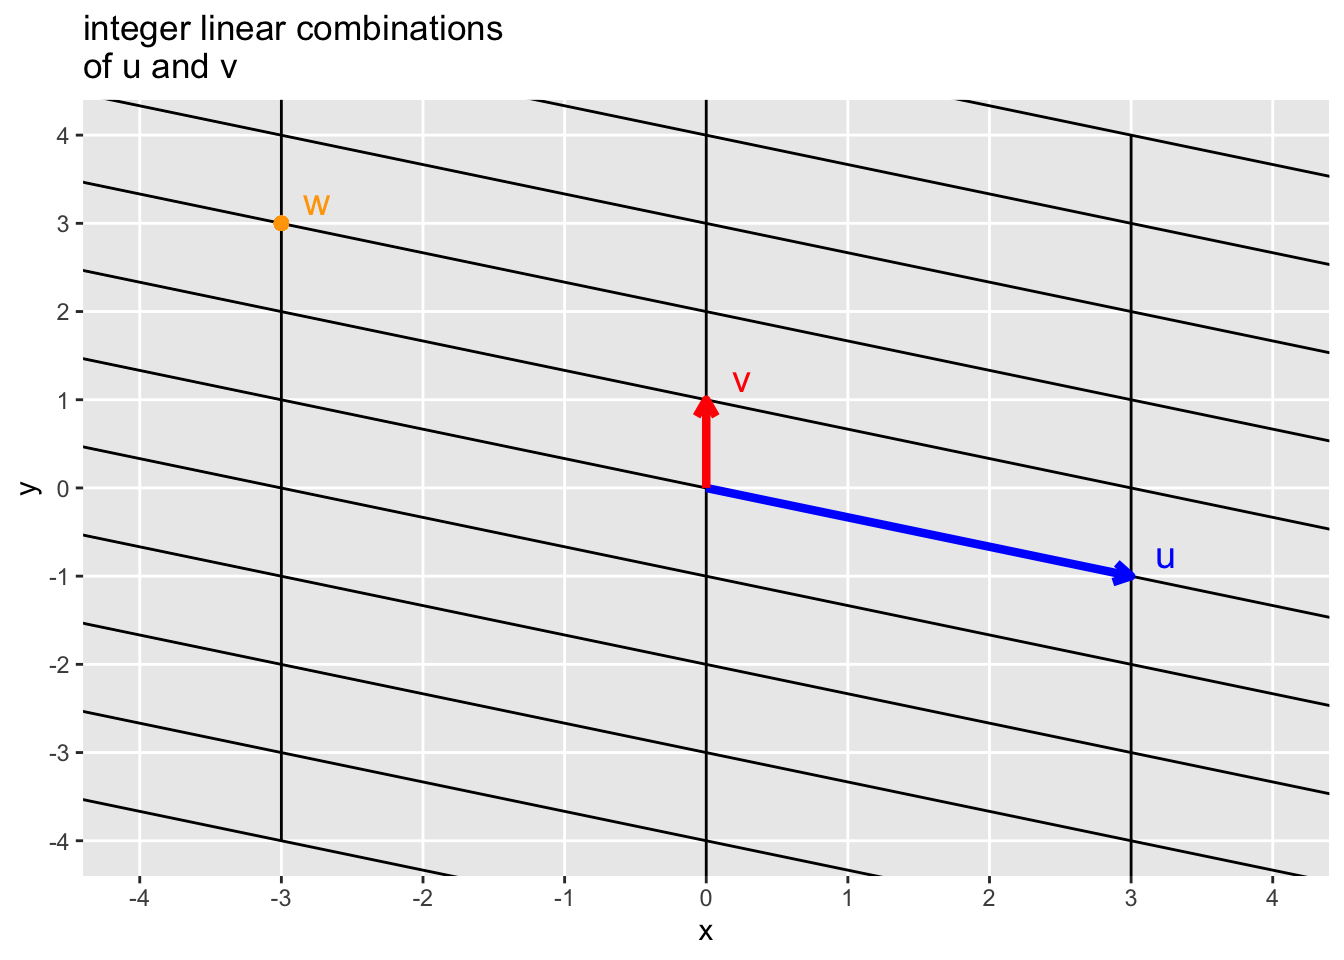
\includegraphics{multivariable-math_files/figure-latex/unnamed-chunk-70-1.pdf}

From the example above, we can answer the question ``Is the point (a, b) on the line defined by the vector \(\mathbf{u}\)?'' by asking whether the point (a, b) is in the \(span\{\mathbf{u}\}\). While this is trivial for such a simple problem, the use of the span will make things easier in higher dimensions.

\begin{itemize}
\tightlist
\item
  \textbf{Example: do in class} 2 3-d vectors that are not scalar multiples of each other define a plane. Does a point lie within the plane? Use the span to answer this question.
\end{itemize}

The shiny app below demonstrates how the concept of span can be understood in 2 dimensions. The app can be downloaded and run

\begin{Shaded}
\begin{Highlighting}[]
\KeywordTok{library}\NormalTok{(shiny)}
\KeywordTok{runGitHub}\NormalTok{(}\DataTypeTok{rep =} \StringTok{"multivariable-math"}\NormalTok{,}
          \DataTypeTok{username =} \StringTok{"jtipton25"}\NormalTok{, }
          \DataTypeTok{subdir =} \StringTok{"shiny-apps/chapter-03/span"}\NormalTok{) }
\end{Highlighting}
\end{Shaded}

\hypertarget{matrix-equation}{%
\chapter{Matrix equations}\label{matrix-equation}}

\begin{Shaded}
\begin{Highlighting}[]
\KeywordTok{library}\NormalTok{(tidyverse)}
\KeywordTok{library}\NormalTok{(dasc2594)}
\KeywordTok{library}\NormalTok{(gg3D)}
\end{Highlighting}
\end{Shaded}

Here we introduce the concept of the linear equation \(\mathbf{A} \mathbf{x} = \mathbf{b}\). This equation is the most fundamental equation in all of statistics and data science. Given a matrix \(\mathbf{A}\) and a vector of constants \(\mathbf{b}\), the goal is to solve for the value (or values) of \(\mathbf{x}\) that are a solution to this equation. The equation \(\mathbf{A} \mathbf{x} = \mathbf{b}\) is a matrix representation of the system of linear equations

\[
\begin{aligned}
\mathbf{A} \mathbf{x} & = \mathbf{b} \\
\begin{pmatrix} \mathbf{a}_1 & \ldots & \mathbf{a}_K \end{pmatrix} \begin{pmatrix} x_1 \\ \vdots \\ x_K \end{pmatrix} & = \mathbf{b} \\
x_1 \mathbf{a}_1 + \ldots + x_K \mathbf{a}_K & = \mathbf{b} \\
\end{aligned}
\label{eq:matrix-equation}
\]

as long as the matrix \(\mathbf{A}\) has \(n\) rows and \(K\) columns and the vectors \(\mathbf{a}_k\) are \(n\)-dimensional.

\begin{itemize}
\item
  \textbf{Example: in class}
\item
  \textbf{Example: in class}
\end{itemize}

\hypertarget{solutions-of-matrix-equations}{%
\section{Solutions of matrix equations}\label{solutions-of-matrix-equations}}

Because the matrix equation \(\mathbf{A} \mathbf{x} = \mathbf{b}\) is equivalent to a linear system of equations \(x_1 \mathbf{a}_1 + \ldots + x_K \mathbf{a}_K = \mathbf{b}\), we can solve the matrix equation \(\mathbf{A} \mathbf{x} = \mathbf{b}\) by writing the equation in an augmented matrix form
\[
\begin{aligned}
\begin{pmatrix} \mathbf{a}_1 & \ldots & \mathbf{a}_K & \mathbf{b} \end{pmatrix}
\end{aligned}
\]
and then reducing the matrix to reduced row echelon form. This gives rise to the theorem

\begin{theorem}
The matrix equation \(\mathbf{A} \mathbf{x} = \mathbf{b}\), the vector equation \(x_1 \mathbf{a}_1 + \ldots + x_K \mathbf{a}_K = \mathbf{b}\), and the augmented matrix \(\begin{pmatrix} \mathbf{a}_1 & \ldots & \mathbf{a}_K & \mathbf{b} \end{pmatrix}\) all have the same solution set.
\end{theorem}

\hypertarget{existence-of-solutions}{%
\section{Existence of solutions}\label{existence-of-solutions}}

A solution to the matrix equation \(\mathbf{A} \mathbf{x} = \mathbf{b}\) exists if and only if \(\mathbf{b}\) is a linear combination of the columns of \(\mathbf{A}\). In other words, \(\mathbf{A} \mathbf{x} = \mathbf{b}\) has a solution if and only if \(\mathbf{b}\) is in the \(\mbox{span}\{\mathbf{a}_1, \ldots, \mathbf{a}_K\}\).

\begin{itemize}
\tightlist
\item
  \textbf{Example: in class} Let \(\mathbf{A} =\ldots\) and \(\mathbf{b} = \ldots\). Is the matrix equation \(\mathbf{A} \mathbf{x} = \mathbf{b}\) consistent?
\end{itemize}

\begin{theorem}

For the \(n \times K\) matrix \(\mathbf{A}\), the following statements are equivalent:

\begin{enumerate}
\def\labelenumi{\alph{enumi})}
\item
  For each \(\mathbf{b} \in \mathcal{R}^n\), the equation \(\mathbf{A} \mathbf{x} = \mathbf{b}\) has at least one solution
\item
  Each \(\mathbf{b} \in \mathcal{R}^n\) is a linear combination of the columns of \(\mathbf{A}\)
\item
  The columns of \(\mathbf{A}\) span \(\mathcal{R}^n\)
\item
  \(\mathbf{A}\) has \(n\) pivot columns. (\(\mathbf{A}\) has a pivot in every row)
\end{enumerate}

\end{theorem}

\hypertarget{matrix-vector-multiplication}{%
\section{Matrix-vector multiplication}\label{matrix-vector-multiplication}}

To calculate \(\mathbf{A} \mathbf{x}\), we need to define matrix multiplication. The equivalence between the linear systems of equations \(x_1 \mathbf{a}_1 + \ldots + x_K \mathbf{a}_K = \mathbf{b}\) and the matrix equation \(\mathbf{A} \mathbf{x}\) gives a hint in how to do this. First, recall the definition of \(\mathbf{A}\) and \(\mathbf{x}\)

\[
\begin{aligned}
\mathbf{A} = \begin{pmatrix}
a_{11} & a_{12} & \ldots & a_{1K} \\
a_{21} & a_{22} & \ldots & a_{2K} \\
\vdots & \vdots & \ddots & \vdots \\
a_{n1} & a_{n2} & \ldots & a_{nK} \\
\end{pmatrix} && \mathbf{x} = \begin{pmatrix} x_1 \\ x_2 \\ \vdots \\ x_K \end{pmatrix}
\end{aligned}
\]
The matrix product \(\mathbf{A}\mathbf{x}\) is the linear system of equations
\[
\begin{aligned}
\mathbf{A}  \mathbf{x} & = \begin{pmatrix}
a_{11} & a_{12} & \ldots & a_{1K} \\
a_{21} & a_{22} & \ldots & a_{2K} \\
\vdots & \vdots & \ddots & \vdots \\
a_{n1} & a_{n2} & \ldots & a_{nK} \\
\end{pmatrix} \begin{pmatrix} x_1 \\ x_2 \\ \vdots \\ x_n \end{pmatrix} \\
& = x_1\begin{pmatrix}
a_{11} \\ a_{21} \\ \vdots \\ a_{n1} 
\end{pmatrix} +
x_2 \begin{pmatrix}
a_{12} \\ a_{22} \\ \vdots \\ a_{n2} 
\end{pmatrix} +
\cdots + x_K \begin{pmatrix}
a_{1K} \\ a_{nK} \\ \vdots \\ a_{nK} \end{pmatrix} \\
& =  \begin{pmatrix}
a_{11} x_1 + a_{12} x_2 + \ldots + a_{1K} x_K \\
a_{21} x_1 + a_{22} x_2 + \ldots + a_{2K} x_K \\
\vdots \\
a_{n1} x_1 + a_{n2} x_2 + \ldots + a_{nK} x_K \\
\end{pmatrix}
\end{aligned}
\]
Notice that the first row of the last matrix above has the sum first row of the matrix \(\mathbf{A}\) multiplied by the corresponding elements in \(\mathbf{x}\) (i.e., first element \(a_{11}\) of the first row of \(\mathbf{A}\) times the first element \(x_1\) of \(\mathbf{x}\) plus the second, third, fourth, etc.). Likewise, this pattern holds for the second row, and all the other rows. This gives an algorithm for evaluating the product \(\mathbf{A} \mathbf{x}\).

\begin{definition}
The product \(\mathbf{A}\mathbf{x}\) of a \(n \times K\) matrix \(\mathbf{A}\) with a \(K\)-vector \(\mathbf{x}\) is a \(n\)-vector where the \(i\)th element of \(\mathbf{A}\mathbf{x}\) is the sum of the \(i\)th row of \(\mathbf{A}\) times the corresponding elements of the vector \(\mathbf{x}\)
\end{definition}

\begin{itemize}
\item
  \textbf{Example: in class}
\item
  \textbf{Example: in class}
\item
  \textbf{Example: in R using loops}
\item
  \textbf{Example: in R using \texttt{\%*\%}}
\end{itemize}

\hypertarget{properties-of-matrix-vector-multiplication}{%
\section{Properties of matrix-vector multiplication}\label{properties-of-matrix-vector-multiplication}}

If \(\mathbf{A}\) is a \(n \times K\) matrix, \(\mathbf{u}\) and \(\mathbf{v}\) are vectors in \(\mathcal{R}^K\) and \(c\) is a scalar, then

\begin{enumerate}
\def\labelenumi{\alph{enumi})}
\tightlist
\item
  \(\mathbf{A} (\mathbf{u} + \mathbf{v}) = \mathbf{A} \mathbf{u} + \mathbf{A} \mathbf{v}\)
\item
  \(\mathbf{A} (c \mathbf{u}) = (c \mathbf{A}) \mathbf{u}\)
\end{enumerate}

\begin{itemize}
\tightlist
\item
  \textbf{Proof in class}
\end{itemize}

\hypertarget{solutions-of-linear-systems-1}{%
\section{Solutions of linear systems}\label{solutions-of-linear-systems-1}}

\hypertarget{homogeneous-linear-systems-of-equations}{%
\subsection{Homogeneous linear systems of equations}\label{homogeneous-linear-systems-of-equations}}

\begin{definition}
The matrix equation
\[
\begin{aligned}
\mathbf{A}\mathbf{x} = \mathbf{0}
\end{aligned}
\label{eq:homogeneous}
\]
is called a homogeneous system of equations. The vector \(\mathbf{0}\) is a vector of length \(N\) composed of all zeros. The \textbf{trivial} solution of the homogeneous equation is when \(\mathbf{x} = \mathbf{0}\) and is not a very useful solution. Typically one is interested in \textbf{nontrivial} solutions where \(\mathbf{x} \neq \mathbf{0}\).
\end{definition}

The homogeneous linear system of equations can be written in augmented matrix form
\[
\begin{aligned}
\begin{pmatrix} \mathbf{a}_1 & \ldots & \mathbf{a}_K & \mathbf{0} \end{pmatrix}
\end{aligned}
\]
which implies that a non-trivial solution only exists if there is a free variable. Another way of saying this is that at least one column \(\mathbf{A}\) must not be a pivot column (Note: the last column of the augmented matrix will not be a pivot column because it will be a column of zeros). If every column of \(\mathbf{A}\) were a pivot column, the reduced row echelon form of the augmented matrix would be
\[
\begin{aligned}
\begin{pmatrix}
1 & 0 & \ldots & 0 & 0 \\
0 & 1 & \ldots & 0 & 0 \\
0 & 0 & \ldots & 1 & 0 
\end{pmatrix}
\end{aligned}
\]
which implies the only solution is the trivial solution \(\mathbf{0}\).

\begin{itemize}
\tightlist
\item
  \textbf{Example: in class}
\end{itemize}

\[
\begin{aligned}
3 x_1 - 2 x_2 + 4 x_3 = 0 \\
- 2 x_1 + 4 x_2 - 2 x_3 = 0 \\
5 x_1 - 6 x_2 + 6 x_3 = 0
\end{aligned}
\]
* \textbf{Example: in class}

Consider the equation

\[
\begin{aligned}
2x_1 + 4 x_2 - x_3 = 0.
\end{aligned}
\]
we can write this as
\[
\begin{aligned}
x_1 = -2 x_2 + \frac{1}{2} x_3
\end{aligned}
\]
where \(x_2\) and \(x_3\) are free variables. Writing this as a solution \(\mathbf{x}\) gives
\[
\begin{aligned}
\mathbf{x} = \begin{pmatrix} x_1 \\ x_2 \\ x_3 \end{pmatrix} = \begin{pmatrix} -2 x_2 + \frac{1}{2} x_3 \\ x_2 \\ x_3 \end{pmatrix} = 
x_2 \begin{pmatrix} -2 \\ 1 \\ 0 \end{pmatrix} + 
x_3 \begin{pmatrix} \frac{1}{2} \\ 0 \\ 1 \end{pmatrix}
\end{aligned}
\]
which is a linear combination of the vectors \(\mathbf{u} = \begin{pmatrix} -2 \\ 1 \\ 0 \end{pmatrix}\) and \(\mathbf{v} = \begin{pmatrix} \frac{1}{2} \\ 0 \\ 1 \end{pmatrix}\). This implies that we can write the solution \(\mathbf{x} = c \mathbf{u} + d \mathbf{v}\) for scalars \(a\) and \(b\). Therefore, the solution set \(\mathbf{x}\) is contained in the \(\mbox{span}\{\mathbf{u}, \mathbf{v}\}\). Because the vectors \(\mathbf{u}\) and \(\mathbf{v}\) are linearly independent (they don't point in the same direction), the set of all linear combinations of \(c \mathbf{u} + d \mathbf{v}\) defines a plane.

\begin{definition}
A solution set of the form \(\mathbf{x} = c \mathbf{u} + d \mathbf{v}\) is called a \textbf{parametric vector solution}.
\end{definition}

\hypertarget{solutions-to-nonhomogeneous-systems}{%
\section{Solutions to nonhomogeneous systems}\label{solutions-to-nonhomogeneous-systems}}

Recall the simple linear equation
\[
y = mx + b
\]
where \(m\) is the slope and \(b\) is the y-intercept. Setting \(b = 0\) gives a simple homogenous linear equation where the y-intercept goes through the origin (0, 0). When \(b\) is nonzero, the line keeps the same slope but is shifted upward/downward by \(b\).

\begin{Shaded}
\begin{Highlighting}[]
\KeywordTok{ggplot}\NormalTok{(}\DataTypeTok{data =} \KeywordTok{data.frame}\NormalTok{(}\DataTypeTok{x =} \DecValTok{0}\NormalTok{, }\DataTypeTok{y =} \DecValTok{0}\NormalTok{), }\KeywordTok{aes}\NormalTok{(x, y)) }\OperatorTok{+}
\StringTok{    }\KeywordTok{geom_vline}\NormalTok{(}\DataTypeTok{xintercept =} \DecValTok{0}\NormalTok{) }\OperatorTok{+}
\StringTok{    }\KeywordTok{geom_hline}\NormalTok{(}\DataTypeTok{yintercept =} \DecValTok{0}\NormalTok{) }\OperatorTok{+}
\StringTok{    }\KeywordTok{geom_abline}\NormalTok{(}\DataTypeTok{slope =} \DecValTok{2}\NormalTok{, }\DataTypeTok{intercept =} \DecValTok{0}\NormalTok{, }\DataTypeTok{color =} \StringTok{"red"}\NormalTok{) }\OperatorTok{+}
\StringTok{    }\KeywordTok{geom_abline}\NormalTok{(}\DataTypeTok{slope =} \DecValTok{2}\NormalTok{, }\DataTypeTok{intercept =} \DecValTok{2}\NormalTok{, }\DataTypeTok{color =} \StringTok{"blue"}\NormalTok{) }\OperatorTok{+}
\StringTok{    }\KeywordTok{coord_cartesian}\NormalTok{(}\DataTypeTok{xlim =} \KeywordTok{c}\NormalTok{(}\OperatorTok{-}\DecValTok{4}\NormalTok{, }\DecValTok{4}\NormalTok{), }\DataTypeTok{ylim =} \KeywordTok{c}\NormalTok{(}\OperatorTok{-}\DecValTok{4}\NormalTok{, }\DecValTok{4}\NormalTok{))  }\OperatorTok{+}
\StringTok{    }\KeywordTok{geom_text}\NormalTok{(}
        \DataTypeTok{data =} \KeywordTok{data.frame}\NormalTok{(}\DataTypeTok{x =} \KeywordTok{c}\NormalTok{(}\DecValTok{0}\NormalTok{, }\DecValTok{0}\NormalTok{), }\DataTypeTok{y =} \KeywordTok{c}\NormalTok{(}\DecValTok{0}\NormalTok{, }\DecValTok{2}\NormalTok{), }\DataTypeTok{text =} \KeywordTok{c}\NormalTok{(}\StringTok{"homogeneous}\CharTok{\textbackslash{}n}\StringTok{solution"}\NormalTok{, }\StringTok{"inhomogeneous}\CharTok{\textbackslash{}n}\StringTok{solution"}\NormalTok{)),}
        \KeywordTok{aes}\NormalTok{(}\DataTypeTok{x =}\NormalTok{ x }\OperatorTok{+}\StringTok{ }\KeywordTok{c}\NormalTok{(}\FloatTok{1.75}\NormalTok{, }\DecValTok{-1}\NormalTok{), }\DataTypeTok{y =}\NormalTok{ y }\OperatorTok{+}\StringTok{ }\FloatTok{0.5}\NormalTok{, }\DataTypeTok{label =}\NormalTok{ text), }\DataTypeTok{size =} \DecValTok{5}\NormalTok{, }\DataTypeTok{inherit.aes =} \OtherTok{FALSE}\NormalTok{,}
        \DataTypeTok{color =} \KeywordTok{c}\NormalTok{(}\StringTok{"red"}\NormalTok{, }\StringTok{"blue"}\NormalTok{)) }\OperatorTok{+}
\StringTok{    }\KeywordTok{geom_segment}\NormalTok{(}
        \KeywordTok{aes}\NormalTok{(}\DataTypeTok{x =} \DecValTok{0}\NormalTok{, }\DataTypeTok{xend =} \DecValTok{0}\NormalTok{, }\DataTypeTok{y =} \DecValTok{0}\NormalTok{, }\DataTypeTok{yend =} \DecValTok{2}\NormalTok{),}
        \DataTypeTok{arrow =} \KeywordTok{arrow}\NormalTok{(}\DataTypeTok{length =} \KeywordTok{unit}\NormalTok{(}\FloatTok{0.1}\NormalTok{, }\StringTok{"inches"}\NormalTok{)), }
        \DataTypeTok{size =} \FloatTok{1.5}\NormalTok{, }\DataTypeTok{color =} \StringTok{"orange"}\NormalTok{) }\OperatorTok{+}
\StringTok{    }\KeywordTok{geom_text}\NormalTok{(}
        \DataTypeTok{data =} \KeywordTok{data.frame}\NormalTok{(}\DataTypeTok{x =} \DecValTok{0}\NormalTok{, }\DataTypeTok{y =} \DecValTok{2}\NormalTok{, }\DataTypeTok{text =} \StringTok{"b"}\NormalTok{),}
        \KeywordTok{aes}\NormalTok{(}\DataTypeTok{x =}\NormalTok{ x }\OperatorTok{+}\StringTok{ }\FloatTok{0.5}\NormalTok{, }\DataTypeTok{y =}\NormalTok{ y, }\DataTypeTok{label =}\NormalTok{ text), }
        \DataTypeTok{size =} \DecValTok{8}\NormalTok{, }\DataTypeTok{inherit.aes =} \OtherTok{FALSE}\NormalTok{,}
        \DataTypeTok{color =} \StringTok{"orange"}\NormalTok{) }
\end{Highlighting}
\end{Shaded}

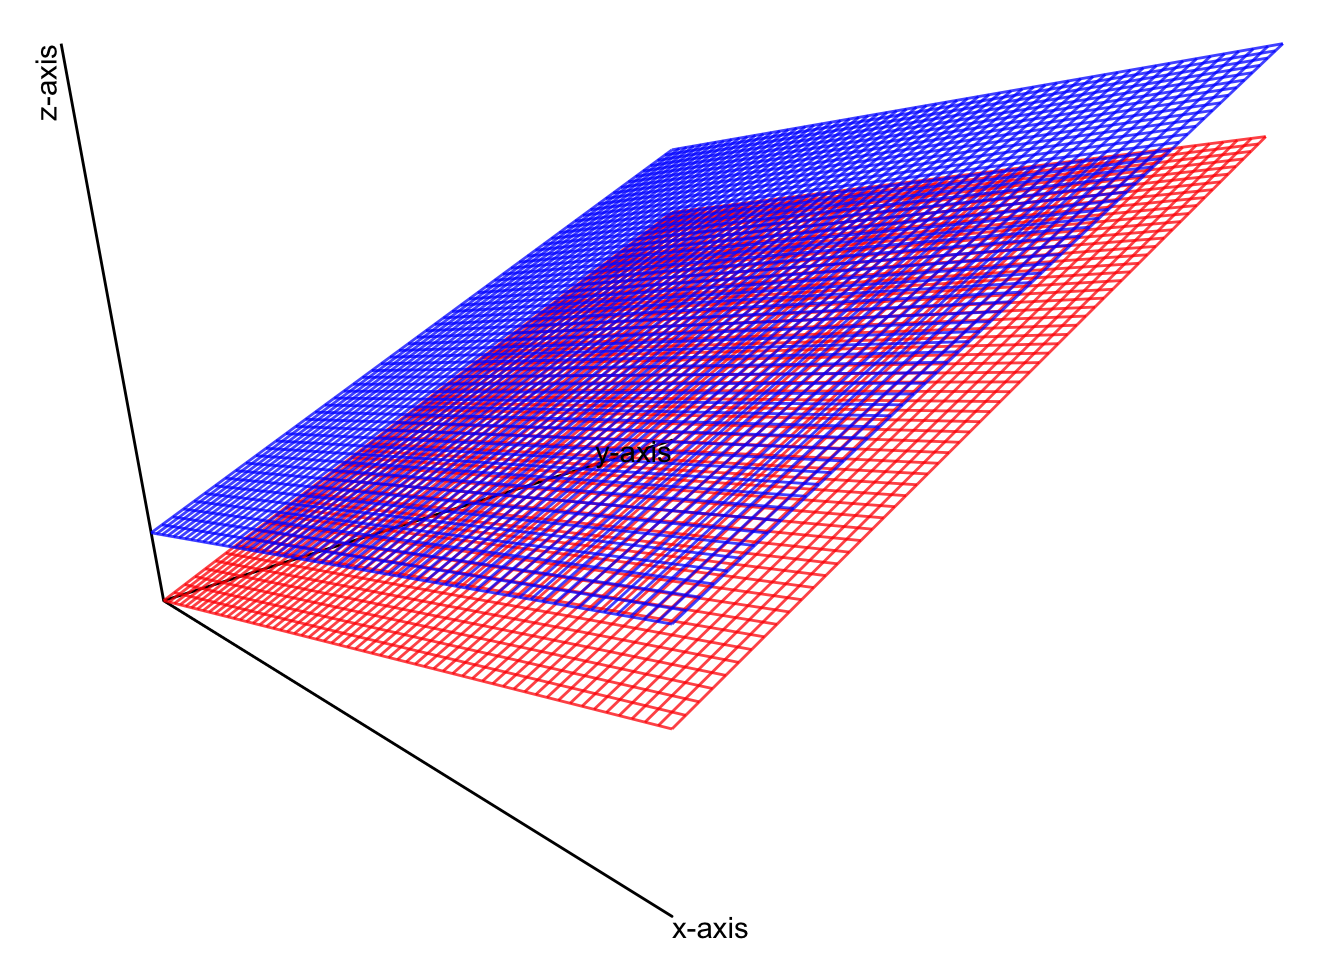
\includegraphics{multivariable-math_files/figure-latex/unnamed-chunk-73-1.pdf}

This shift in location (but not in slope) is called a \textbf{translation}

\begin{itemize}
\tightlist
\item
  \textbf{Example:} Show this shift for a system of linear equations where the solution set defines a plane. From example above,
  \[
  \begin{aligned}
  2x_1 + 4 x_2 - x_3 = 0.
  \end{aligned}
  \]
  has the parametric solution \(\mathbf{x} = c \mathbf{u} + d \mathbf{v}\) with
  \[
  \begin{aligned}
  \mathbf{u} & = \begin{pmatrix} -2 \\ 1 \\ 0 \end{pmatrix} &
  \mathbf{v} & = \begin{pmatrix} \frac{1}{2} \\ 0 \\ 1 \end{pmatrix}
  \end{aligned}
  \]
\end{itemize}

Now, if we change the system of linear equations so that we have the inhomogeneous equation
\[
\begin{aligned}
2x_1 + 4 x_2 - x_3 = 20.
\end{aligned}
\]
we get the homogeneous solution set \(x_1 = -2 x_2 + \frac{1}{2} x_3 + 10\) which can be written in parametric form as \(\mathbf{x} = c \mathbf{u} + d \mathbf{v} + \mathbf{p}\) with
\[
\begin{aligned}
\mathbf{u} & = \begin{pmatrix} -2 \\ 1 \\ 0 \end{pmatrix} & 
\mathbf{v} & = \begin{pmatrix} \frac{1}{2} \\ 0 \\ 1 \end{pmatrix} & 
\mathbf{p} & = \begin{pmatrix} 10 \\ 0 \\ 0 \end{pmatrix}
\end{aligned}
\]

For plotting, we will solve these equations for \(x_3\), letting \(x_1\) and \(x_2\) be free variables (this is just for the requirements of the plotting function). Thus, the homogeneous equation has the solution \(x_3 = 2x_1 + 4x_2\) and the inhomogenous equation has the solution \(x_3 = 2x_1 + 4x_2 - 20\).

\begin{Shaded}
\begin{Highlighting}[]
\CommentTok{# uses gg3D library}
\NormalTok{n <-}\StringTok{ }\DecValTok{60}
\NormalTok{x1 <-}\StringTok{ }\NormalTok{x2 <-}\StringTok{ }\KeywordTok{seq}\NormalTok{(}\OperatorTok{-}\DecValTok{10}\NormalTok{, }\DecValTok{10}\NormalTok{, }\DataTypeTok{length =}\NormalTok{ n)}
\NormalTok{region <-}\StringTok{ }\KeywordTok{expand.grid}\NormalTok{(}\DataTypeTok{x1 =}\NormalTok{ x1, }\DataTypeTok{x2 =}\NormalTok{ x2)}
\NormalTok{df <-}\StringTok{ }\KeywordTok{data.frame}\NormalTok{(}
    \DataTypeTok{x1 =}\NormalTok{ region}\OperatorTok{$}\NormalTok{x1,}
    \DataTypeTok{x2 =}\NormalTok{ region}\OperatorTok{$}\NormalTok{x2,}
    \DataTypeTok{x3 =} \KeywordTok{c}\NormalTok{(}
        \DecValTok{2} \OperatorTok{*}\StringTok{ }\NormalTok{region}\OperatorTok{$}\NormalTok{x1 }\OperatorTok{+}\StringTok{ }\DecValTok{4} \OperatorTok{*}\StringTok{ }\NormalTok{region}\OperatorTok{$}\NormalTok{x2,}
        \DecValTok{2} \OperatorTok{*}\StringTok{ }\NormalTok{region}\OperatorTok{$}\NormalTok{x1 }\OperatorTok{+}\StringTok{ }\DecValTok{4} \OperatorTok{*}\StringTok{ }\NormalTok{region}\OperatorTok{$}\NormalTok{x2 }\OperatorTok{-}\StringTok{ }\DecValTok{20}\NormalTok{),}
    \DataTypeTok{equation =} \KeywordTok{rep}\NormalTok{(}\KeywordTok{c}\NormalTok{(}\StringTok{"inhomogeneous"}\NormalTok{, }\StringTok{"homogeneous"}\NormalTok{), }\DataTypeTok{each =}\NormalTok{ n}\OperatorTok{^}\DecValTok{2}\NormalTok{))}

\CommentTok{# theta and phi set up the "perspective/viewing angle" of the 3D plot}
\NormalTok{theta <-}\StringTok{ }\DecValTok{45}
\NormalTok{phi <-}\StringTok{ }\DecValTok{20}
\KeywordTok{ggplot}\NormalTok{(df, }\KeywordTok{aes}\NormalTok{(}\DataTypeTok{x =}\NormalTok{ x1, }\DataTypeTok{y =}\NormalTok{ x2, }\DataTypeTok{z =}\NormalTok{ x3, }\DataTypeTok{color =}\NormalTok{ equation)) }\OperatorTok{+}
\StringTok{    }\KeywordTok{axes_3D}\NormalTok{(}\DataTypeTok{theta =}\NormalTok{ theta, }\DataTypeTok{phi =}\NormalTok{ phi) }\OperatorTok{+}
\StringTok{    }\KeywordTok{stat_wireframe}\NormalTok{(}
        \DataTypeTok{alpha =} \FloatTok{0.75}\NormalTok{,}
        \DataTypeTok{theta =}\NormalTok{ theta, }\DataTypeTok{phi =}\NormalTok{ phi) }\OperatorTok{+}
\StringTok{    }\KeywordTok{scale_color_manual}\NormalTok{(}\DataTypeTok{values =} \KeywordTok{c}\NormalTok{(}\StringTok{"inhomogeneous"}\NormalTok{ =}\StringTok{ "blue"}\NormalTok{, }\StringTok{"homogeneous"}\NormalTok{ =}\StringTok{ "red"}\NormalTok{)) }\OperatorTok{+}
\StringTok{    }\KeywordTok{theme_void}\NormalTok{() }\OperatorTok{+}
\StringTok{    }\KeywordTok{labs_3D}\NormalTok{(}\DataTypeTok{hjust=}\KeywordTok{c}\NormalTok{(}\DecValTok{0}\NormalTok{,}\DecValTok{1}\NormalTok{,}\DecValTok{1}\NormalTok{), }\DataTypeTok{vjust=}\KeywordTok{c}\NormalTok{(}\DecValTok{1}\NormalTok{, }\DecValTok{1}\NormalTok{, }\FloatTok{-0.2}\NormalTok{), }
            \DataTypeTok{angle=}\KeywordTok{c}\NormalTok{(}\DecValTok{0}\NormalTok{, }\DecValTok{0}\NormalTok{, }\DecValTok{90}\NormalTok{), }\DataTypeTok{theta =}\NormalTok{ theta, }\DataTypeTok{phi =}\NormalTok{ phi) }
\end{Highlighting}
\end{Shaded}

\begin{verbatim}
## Warning: Removed 4 row(s) containing missing values (geom_path).
\end{verbatim}

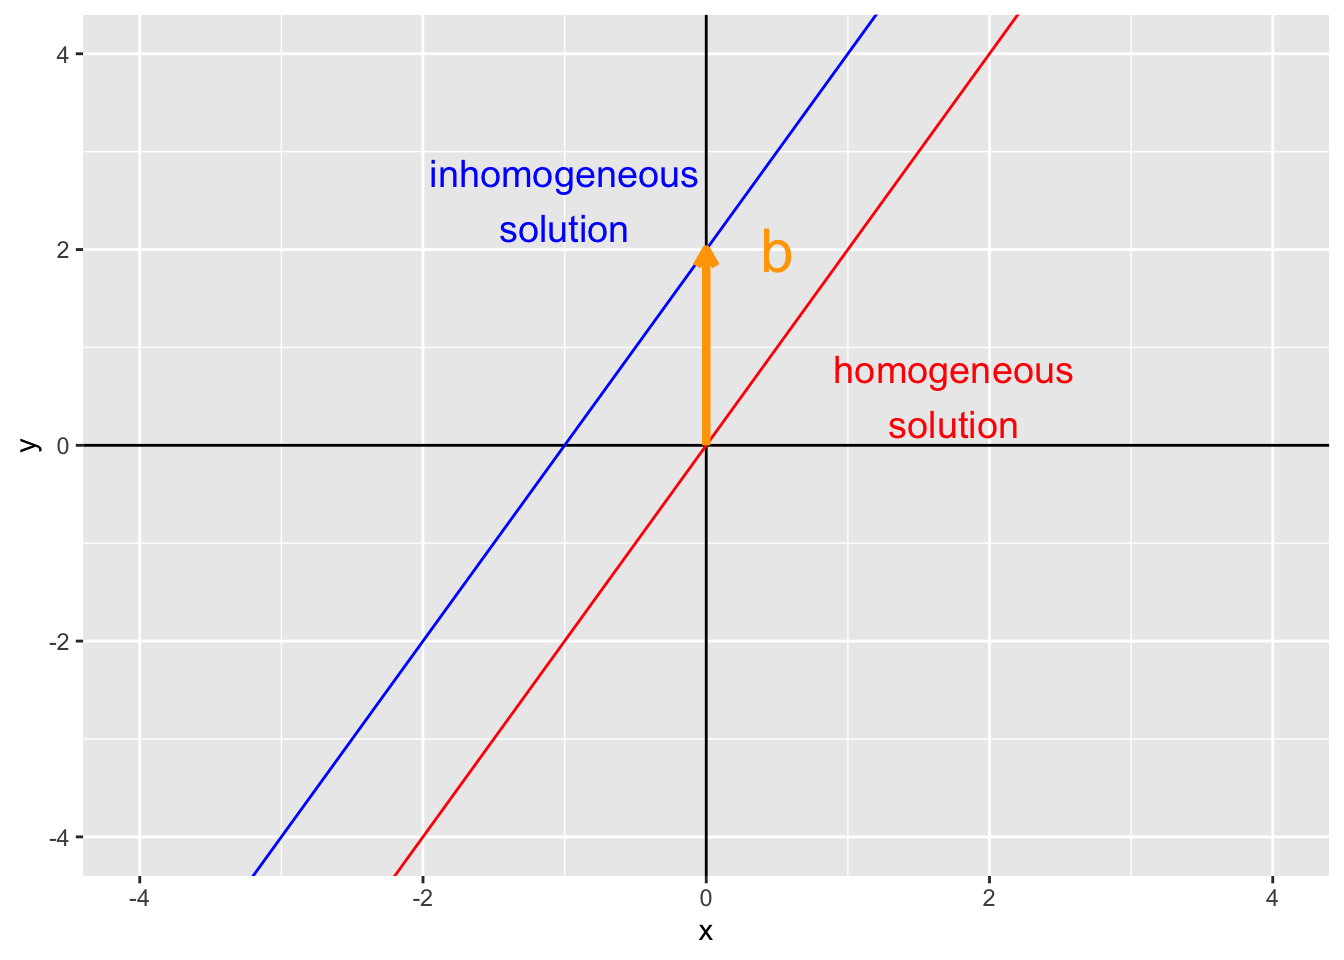
\includegraphics{multivariable-math_files/figure-latex/unnamed-chunk-74-1.pdf}

\begin{itemize}
\tightlist
\item
  \textbf{Example: in class}
  Let's revisit the example from before
\end{itemize}

\[
\begin{aligned}
3 x_1 - 2 x_2 + 4 x_3 = 0 \\
- 2 x_1 + 4 x_2 - 2 x_3 = 0 \\
5 x_1 - 6 x_2 + 6 x_3 = 0
\end{aligned}
\]
but change this so that \(\mathbf{b} = \begin{pmatrix} 2 \\ -6 \\ 8 \end{pmatrix}\)

\begin{itemize}
\tightlist
\item
  \textbf{Write this as a parametric solution with a mean shift}
\end{itemize}

\begin{Shaded}
\begin{Highlighting}[]
\NormalTok{A <-}\StringTok{ }\KeywordTok{matrix}\NormalTok{(}\KeywordTok{c}\NormalTok{(}\DecValTok{3}\NormalTok{, }\DecValTok{-2}\NormalTok{, }\DecValTok{5}\NormalTok{, }\DecValTok{-2}\NormalTok{, }\DecValTok{4}\NormalTok{, }\DecValTok{-6}\NormalTok{, }\DecValTok{4}\NormalTok{, }\DecValTok{-2}\NormalTok{, }\DecValTok{6}\NormalTok{, }\DecValTok{2}\NormalTok{, }\DecValTok{-6}\NormalTok{, }\DecValTok{8}\NormalTok{), }\DecValTok{3}\NormalTok{, }\DecValTok{4}\NormalTok{)}
\KeywordTok{rref}\NormalTok{(A)}
\end{Highlighting}
\end{Shaded}

\begin{verbatim}
##      [,1] [,2] [,3]  [,4]
## [1,]    1    0 1.50 -0.50
## [2,]    0    1 0.25 -1.75
## [3,]    0    0 0.00  0.00
\end{verbatim}

\[
\begin{aligned}
x_1 = \frac{3}{2} x_2  - \frac{1}{2}\\
x_2 = \frac{1}{4} x_3  - \frac{7}{4} \\
\end{aligned}
\]
which was the same solution set as the homoegenous solution plus the additional vector \(\begin{pmatrix} -\frac{1}{2} \\ -\frac{7}{4} \\ 0 \end{pmatrix}\). Thus, the inhomogenous solution is now \(\mathbf{x} = c \mathbf{u} + d \mathbf{v} + \mathbf{p}\) where
\[
\begin{aligned}
\mathbf{u} &= \begin{pmatrix} 1 \\ 0 \\ \frac{3}{2} \end{pmatrix} & 
\mathbf{v} &= \begin{pmatrix} 0 \\ 1 \\ \frac{1}{4} \end{pmatrix} & 
\mathbf{p} &= \begin{pmatrix} -\frac{1}{2} \\ -\frac{7}{4} \\ 0 \end{pmatrix} 
\end{aligned}
\]

\hypertarget{finding-solutions}{%
\section{Finding solutions}\label{finding-solutions}}

The following algorithm describes how to solve a linear system of equations.

\begin{enumerate}
\def\labelenumi{\arabic{enumi})}
\item
  Put the system of equations in an augmented matrix form
\item
  Reduce the augmented matrix to reduced row echelon form
\item
  Express each determined variable as a function of the free variables.
\item
  Write the solution in a general form where the determined variables are a function of the independent variables
\item
  Decompose the solution \(\mathbf{x}\) into a linear combination of free variables as parameters
\end{enumerate}

\hypertarget{linear-independence}{%
\chapter{Linear independence}\label{linear-independence}}

Recall the homogeneous equation \(\mathbf{A} \mathbf{x} = \mathbf{0}\) can be written as a linear combination of coefficients \(x_1, \ldots, x_K\) and vectors \(\mathbf{a}_1, \ldots, \mathbf{a}_K\) where
\[
\begin{aligned}
\sum_{k=1}^K x_k \mathbf{a}_k = \mathbf{0}
\end{aligned}
\]

\begin{definition}
The set of vectors \(\mathbf{a}_1, \ldots, \mathbf{a}_K\) are called \textbf{linearly independent} if the only solution to the vector equation \(\sum_{k=1}^K x_k \mathbf{a}_k = \mathbf{0}\) is the trivial solution. The set of vectors \(\mathbf{a}_1, \ldots, \mathbf{a}_K\) are called \textbf{linearly dependent} if there are coefficients \(x_1, \ldots, x_K\) that are not all zero.
\end{definition}

\begin{example}
\textbf{In class}
\end{example}

What does it mean for a set of vectors to be \textbf{linearly dependent}? This means that there is at least one vector \(\mathbf{a}_k\) that can be written as a sum of the other vectors with coefficients \(x_k\):
\[
\begin{aligned}
\mathbf{a}_k = \sum_{j \neq k} x_{j} \mathbf{a}_{j}
\end{aligned}
\]
Note: \textbf{linear dependence} does not imply that all vectors \(\mathbf{a}_{k}\) can be written as a linear combination of other vectors, just that there is at least one such vector in the set.

\begin{example}
\textbf{Example: in class -- determine if the vectors are linearly independent and solve the dependence relation}
\end{example}

\begin{theorem}
The matrix \(\mathbf{A}\) has linearly independent columns if and only if the matrix equation \(\mathbf{A}\mathbf{x} = \mathbf{0}\) has only the trivial solution.
\end{theorem}

\begin{example}
\textbf{Example: in class} A set of a single vector
\end{example}

\begin{example}

\textbf{Example: in class} A set of two vectors

\begin{itemize}
\item
  linearly independent if:
\item
  linearly dependent if one vector is a scalar multiple of the other:
\end{itemize}

\end{example}

\begin{theorem}
If an \(n \times K\) matrix \(\mathbf{A}\) has \(K > n\), then the columns of \(\mathbf{A}\) are linearly dependent. In other words, if a set of vectors \(\mathbf{a}_1, \ldots, \mathbf{a}_K\) contains more vectors than entries within vectors, the set of vectors is linearly dependent.
\end{theorem}

\begin{proof}
If \(K>n\), there are more variables (\(K\)) than equations (\(n\)). Therefore, there is at least one free variable and this implies that the homogeneous equation \(\mathbf{A}\mathbf{x}=\mathbf{0}\) has a non-trivial solution \eqref{eq:homogeneous}
\end{proof}

\begin{theorem}
If a set of vectors \(\mathbf{a}_1, \ldots, \mathbf{a}_K\) contains the \(\mathbf{0}\) vector, then the the set of vectors is linearly dependent.
\end{theorem}

\begin{proof}
\textbf{in class}
\end{proof}

\begin{example}
In class: Determine whether the following sets of vectors are linearly dependent
\end{example}

\hypertarget{linear-transformations}{%
\chapter{Linear Transformations}\label{linear-transformations}}

\begin{itemize}
\item
  \href{https://www.3blue1brown.com/lessons/linear-transformations}{3 Blue 1 Brown -- Linear transformations}
\item
  \href{https://www.3blue1brown.com/lessons/3d-transformations}{3 Blue 1 Brown -- 3D transformations}
\end{itemize}

\begin{Shaded}
\begin{Highlighting}[]
\KeywordTok{library}\NormalTok{(tidyverse)}
\KeywordTok{library}\NormalTok{(dasc2594)}
\KeywordTok{library}\NormalTok{(gifski)}
\end{Highlighting}
\end{Shaded}

It is often useful to think of \(\mathbf{A}\mathbf{x}\) as a linear transformation defined by the matrix \(\mathbf{A}\) applied to the vector \(\mathbf{x}\).

A linear transformation is mathematically defined as a function/mapping \(T(\cdot)\) (\(T\) for transformation) from a \textbf{domain} in \(\mathcal{R}^n\) (function input) to a \textbf{codomain} in \(\mathcal{R}^m\) (function output). In shorthand, this is written as \(T:\mathcal{R}^n \rightarrow \mathcal{R}^m\) which is read a ``\(T\) maps inputs from the domain \(\mathcal{R}^n\) to the codomain \(\mathcal{R}^m\).'' For each \(\mathbf{x} \in \mathcal{R}^n\) (in the domain), \(T(\mathbf{x}) \in \mathcal{R}^m\) is known as the image of \(\mathbf{x}\). The set of all \(T(\mathbf{x})\) for all \(\mathbf{x} \in \mathcal{R}^n\) is known as the range of \(T(\mathbf{x})\). Note that it is possible that the range of \(T(\mathbf{x})\) is not required to be the entire space \(\mathcal{R}^m\) (i.e., the range of the transformation \(T\) might be a subset of \(\mathcal{R}^m\))

\textbf{Draw figure}

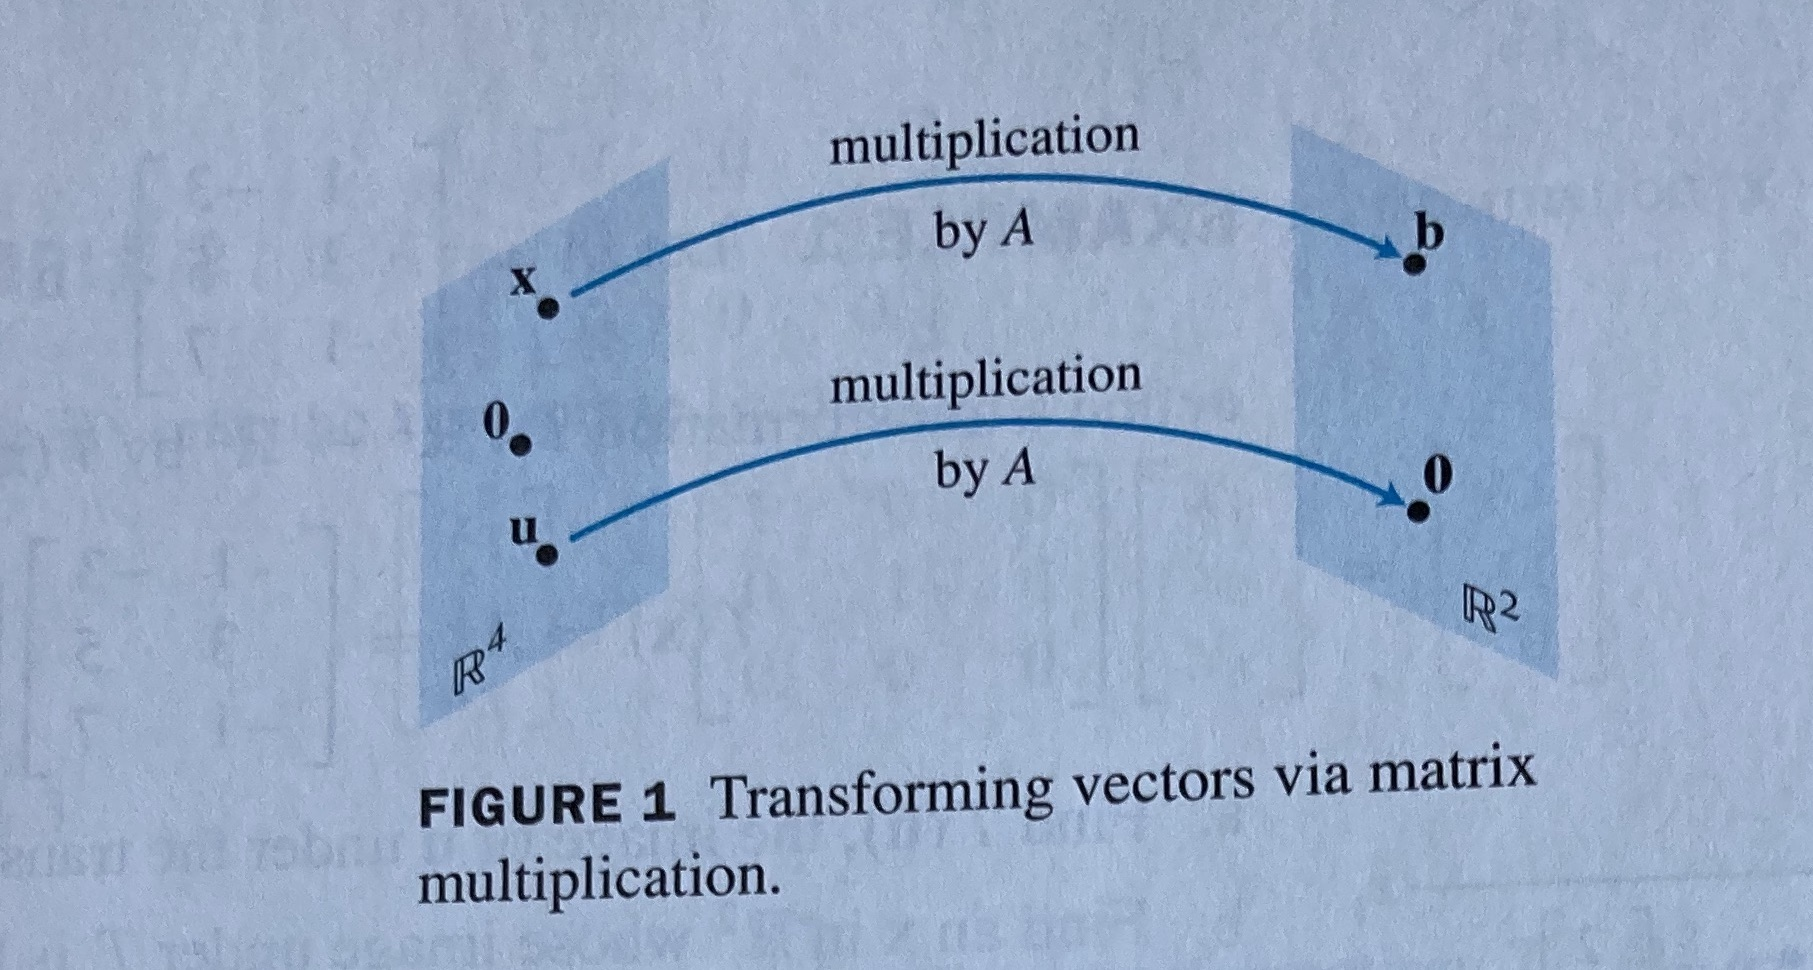
\includegraphics[width=1\linewidth]{/Users/runner/work/multivariable-math/multivariable-math/images/transformation-1}

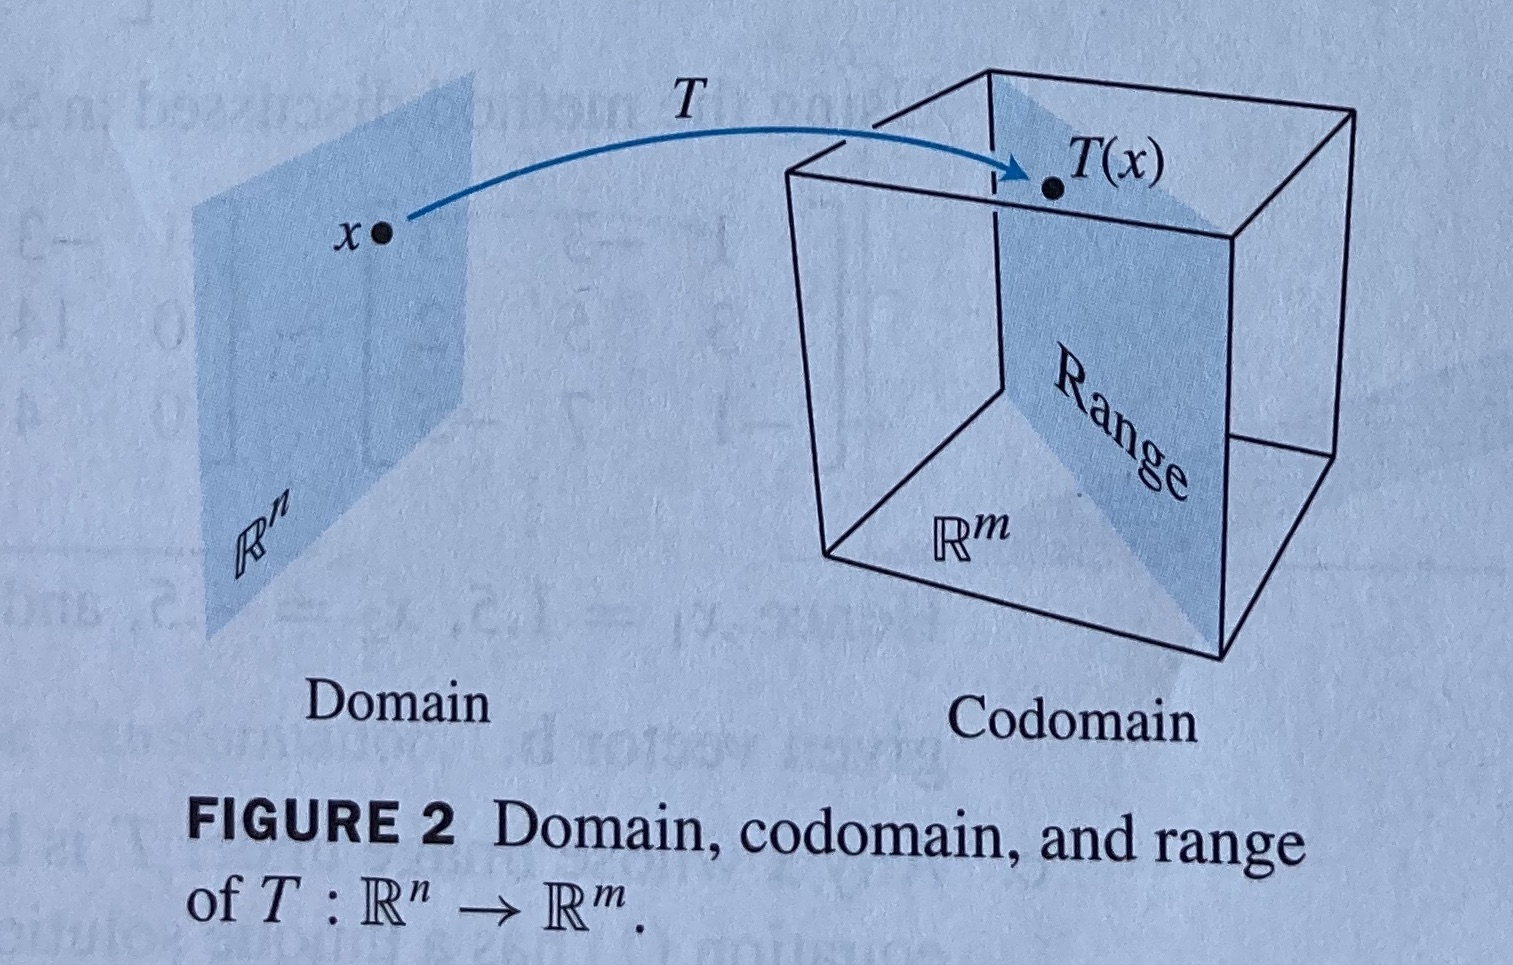
\includegraphics[width=1\linewidth]{/Users/runner/work/multivariable-math/multivariable-math/images/transformation-2}

In the case of matrix transformations (linear transformations), the function \(T(\mathbf{x}) = \mathbf{A} \mathbf{x}\) where \(\mathbf{A}\) is a \(m \times n\) matrix and \(\mathbf{x} \in \mathcal{R}^n\) is a \(n\)-vector.

\begin{itemize}
\tightlist
\item
  \textbf{Question:} What kind of object is \(\mathbf{A} \mathbf{x}\)?

  \begin{itemize}
  \tightlist
  \item
    scalar
  \item
    vector
  \item
    matrix
  \item
    array
  \end{itemize}
\item
  \textbf{Question} What are the dimensions of \(\mathbf{A} \mathbf{x}\)?
\end{itemize}

Using the matrix transformation notation, the domain of the transformation \(T\) is \(\mathcal{R}^n\), the codomain of \(\mathcal{T}\) \(\mathcal{R}^m\). The range of the transformation \(T\) is the set of all linear combinations of the columns of \(\mathbf{A}\) (the \(\mbox{span}\{\mathbf{a}_1, \ldots, \mathbf{a}_n\}\)) because the transformation \(T(\mathbf{x}) = \mathbf{A} \mathbf{x}\) is a linear combination \(\sum_{i=1}^n x_i \mathbf{a}_i\) of the columns \(\{\mathbf{a}_i\}_{i=1}^n\) of \(\mathbf{A}\) with coefficients \(x_1, \ldots, x_n\)

\begin{example}
\[
\begin{aligned}
\mathbf{A} = \begin{pmatrix}
2 & 4 \\
-3 & 1 \\
-1 & 6
\end{pmatrix}
&& \mathbf{u} = \begin{pmatrix}
1 \\
3
\end{pmatrix}
&& \mathbf{b} = \begin{pmatrix}
-2 \\
-11 \\
-15
\end{pmatrix} &&
\mathbf{c} = \begin{pmatrix}
2 \\
-2 \\
-1
\end{pmatrix}
\end{aligned}
\]

\begin{Shaded}
\begin{Highlighting}[]
\NormalTok{A <-}\StringTok{ }\KeywordTok{matrix}\NormalTok{(}\KeywordTok{c}\NormalTok{(}\DecValTok{2}\NormalTok{, }\DecValTok{-3}\NormalTok{, }\DecValTok{-1}\NormalTok{, }\DecValTok{4}\NormalTok{, }\DecValTok{1}\NormalTok{, }\DecValTok{6}\NormalTok{), }\DecValTok{3}\NormalTok{, }\DecValTok{2}\NormalTok{)}
\NormalTok{u <-}\StringTok{ }\KeywordTok{c}\NormalTok{(}\DecValTok{1}\NormalTok{, }\DecValTok{3}\NormalTok{)}
\NormalTok{b <-}\StringTok{ }\DecValTok{3} \OperatorTok{*}\StringTok{ }\NormalTok{A[, }\DecValTok{1}\NormalTok{] }\OperatorTok{-}\StringTok{ }\DecValTok{2} \OperatorTok{*}\StringTok{ }\NormalTok{A[, }\DecValTok{2}\NormalTok{]}
\NormalTok{c <-}\StringTok{ }\KeywordTok{c}\NormalTok{(}\DecValTok{2}\NormalTok{, }\DecValTok{-2}\NormalTok{, }\DecValTok{-1}\NormalTok{)}
\end{Highlighting}
\end{Shaded}

\begin{enumerate}
\def\labelenumi{\alph{enumi})}
\tightlist
\item
  Find the image of \(\mathbf{u}\) using the matrix transformation \(T\) (e.g., calculate \(T(\mathbf{u})\)).
\end{enumerate}

\begin{Shaded}
\begin{Highlighting}[]
\CommentTok{# a}
\NormalTok{A }\OperatorTok\StringTok{ }\NormalTok{u}
\end{Highlighting}
\end{Shaded}

\begin{verbatim}
##      [,1]
## [1,]   14
## [2,]    0
## [3,]   17
\end{verbatim}

The image of \(\mathbf{u}\) under \(T\) is \(T(\mathbf{u}) = \mathbf{A} \mathbf{u} = \begin{pmatrix} 14 \\ 0 \\ 17 \end{pmatrix}\).

\begin{enumerate}
\def\labelenumi{\alph{enumi})}
\setcounter{enumi}{1}
\tightlist
\item
  Find a coefficient vector \(\mathbf{x} \in \mathcal{R}^2\) such that \(T(\mathbf{x}) = \mathbf{b}\).
\end{enumerate}

\begin{Shaded}
\begin{Highlighting}[]
\CommentTok{#b}
\KeywordTok{rref}\NormalTok{(}\KeywordTok{cbind}\NormalTok{(A, b))}
\end{Highlighting}
\end{Shaded}

\begin{verbatim}
##           b
## [1,] 1 0  3
## [2,] 0 1 -2
## [3,] 0 0  0
\end{verbatim}

A coefficient vector \(\mathbf{x}\) such that \(T(\mathbf{x}) = \mathbf{b}\) is the solution to the matrix equation \(\mathbf{A} \mathbf{x} = \mathbf{b}\) which can be found from the reduced row echelon form of the augmented matrix above giving \(\mathbf{x} = \begin{pmatrix} 3 \\ -2 \end{pmatrix}\)

\begin{enumerate}
\def\labelenumi{\alph{enumi})}
\setcounter{enumi}{2}
\tightlist
\item
  Is there more than one \(\mathbf{x}\) whose image under \(T\) is \(\mathbf{b}?\) In other words, is the solution \(\mathbf{A} \mathbf{x}= \mathbf{b}\) unique?
\end{enumerate}

Use the reduced row echelon form of the matrix equation \(\mathbf{A} \mathbf{x} = \mathbf{b}\) above which gives a unique solution as every (non augmented) column is a pivot. Thus, there is only one solution.

\begin{enumerate}
\def\labelenumi{\alph{enumi})}
\setcounter{enumi}{3}
\tightlist
\item
  Determine if \(\mathbf{c}\) is in the range of \(T\). In other words, does the solution \(\mathbf{A} \mathbf{x}= \mathbf{c}\) exist?
\end{enumerate}

\begin{Shaded}
\begin{Highlighting}[]
\CommentTok{# d}
\KeywordTok{rref}\NormalTok{(}\KeywordTok{cbind}\NormalTok{(A, c)) }\CommentTok{# no because this is an inconsistent system of equations}
\end{Highlighting}
\end{Shaded}

\begin{verbatim}
##          c
## [1,] 1 0 0
## [2,] 0 1 0
## [3,] 0 0 1
\end{verbatim}

The solution to the matrix equation \(\mathbf{A} \mathbf{x} = \mathbf{c}\) which can be found from the reduced row echelon form of the augmented matrix above results in no solution because the last column (the augmented column) is a pivot column. Thus, the system of equations is inconsistent and \(\mathbf{c}\) cannot be written as a linear combination of the columns of \(\mathbf{A}\) which means that \(\mathbf{c}\) is not in the range of \(T\).
\end{example}

\hypertarget{linear-transformations-1}{%
\section{Linear Transformations}\label{linear-transformations-1}}

\begin{definition}

A transformation \(T:\mathcal{R}^n \rightarrow \mathcal{R}^m\) is linear if

\begin{enumerate}
\def\labelenumi{\arabic{enumi})}
\item
  \(T(\mathbf{u} + \mathbf{v}) = T(\mathbf{u}) + T(\mathbf{v})\) for all \(\mathbf{u}\) and \(\mathbf{v}\) in the domain of \(T\)
\item
  \(T(c \mathbf{u}) = c T(\mathbf{u})\) for all scalars \(c\) and all vectors \(\mathbf{u}\) in the domain of \(T\)
\end{enumerate}

\end{definition}

Note: Because a linear transformation is equivalent to a matrix transformation, the definition above is equivalent to the following matrix-vector multiplication properties

If \(\mathbf{A}\) is a \(m \times n\) matrix, \(\mathbf{u}\) and \(\mathbf{v}\) are vectors in \(\mathcal{R}^m\) and \(c\) is a scalar, then

\begin{enumerate}
\def\labelenumi{\arabic{enumi})}
\tightlist
\item
  \(\mathbf{A} (\mathbf{u} + \mathbf{v}) = \mathbf{A} \mathbf{u} + \mathbf{A} \mathbf{v}\)
\item
  \(\mathbf{A} (c \mathbf{u}) = (c \mathbf{A}) \mathbf{u}\)
\end{enumerate}

As a consequence of the previous definition, the following properties hold for scalars \(c\) and \(d\) and vectors \(\mathbf{u}\) and \(\mathbf{v} \in \mathcal{R}^m\)

\begin{enumerate}
\def\labelenumi{\arabic{enumi})}
\setcounter{enumi}{2}
\tightlist
\item
  \(T(\mathbf{0}) = \mathbf{0}\)
\item
  \(T(c \mathbf{u} + d \mathbf{v}) = c T(\mathbf{u}) + d T(\mathbf{v})\)
\end{enumerate}

\begin{itemize}
\tightlist
\item
  \textbf{Show why in class}
\end{itemize}

These properties give rise to the following statement for scalars \(c_1, \ldots, c_m\) and vectors \(\mathbf{u}_1, \ldots, \mathbf{u}_m \in \mathcal{R}^n\)

\begin{enumerate}
\def\labelenumi{\arabic{enumi})}
\setcounter{enumi}{4}
\tightlist
\item
  \(T(c_1 \mathbf{u}_1 + \ldots + c_m \mathbf{u}_m) = c_1 T(\mathbf{u}_1) + \ldots + c_m T(\mathbf{u}_m)\)
\end{enumerate}

The statements above for linear transformations are equivalent to the matrix statements where \(\mathbf{A}\) is a \(m \times n\) matrix, \(\mathbf{u}\) and \(\mathbf{v}\) are vectors in \(\mathcal{R}^m\) and \(c\) is a scalar:

\begin{enumerate}
\def\labelenumi{\arabic{enumi})}
\setcounter{enumi}{2}
\tightlist
\item
  \(\mathbf{A} \mathbf{0} = \mathbf{0}\)
\item
  \(\mathbf{A}(c \mathbf{u} + d \mathbf{v}) = c \mathbf{A} \mathbf{u} + d \mathbf{A} \mathbf{v}\)
\end{enumerate}

And for a \(m \times n\) matrix \(\mathbf{A}\), scalars \(c_1, \ldots, c_m\), and vectors \(\mathbf{u}_1, \ldots, \mathbf{u}_m \in \mathcal{R}^n\)

\begin{enumerate}
\def\labelenumi{\arabic{enumi})}
\setcounter{enumi}{4}
\tightlist
\item
  \(\mathbf{A}(c_1 \mathbf{u}_1 + \ldots + c_m \mathbf{u}_m) = c_1 \mathbf{A}\mathbf{u}_1 + \ldots + c_m \mathbf{A} \mathbf{u}_m\)
\end{enumerate}

\hypertarget{types-of-matrix-transformations}{%
\section{Types of matrix transformations}\label{types-of-matrix-transformations}}

The basic types of matrix transformations include

\begin{enumerate}
\def\labelenumi{\arabic{enumi})}
\tightlist
\item
  contractions/expansions
\item
  rotations
\item
  reflections
\item
  shears
\item
  projections
\end{enumerate}

For the following examples, we will consider the unit vectors \(\mathbf{u} = \begin{pmatrix} 1 \\ 0 \end{pmatrix}\) and \(\mathbf{v} = \begin{pmatrix} 0 \\ 1 \end{pmatrix}\) and apply different linear transformations using the matrix \(\mathbf{A}\).

To build the matrix transformations, we use the \texttt{dasc2594} package and build matrix transformations based on code from \url{https://www.bryanshalloway.com/2020/02/20/visualizing-matrix-transformations-with-gganimate/}.

\hypertarget{contractionsexpansions}{%
\subsection{Contractions/Expansions}\label{contractionsexpansions}}

\hypertarget{horizonal-expansion}{%
\subsubsection{Horizonal Expansion}\label{horizonal-expansion}}

The matrix below gives a horizontal expansion when \(x > 1\)

\[
\mathbf{A} = \begin{pmatrix}
x & 0 \\
0 & 1
\end{pmatrix}
\]

\begin{itemize}
\tightlist
\item
  In the example below, we set \(x = 2\) and generate the transformation.
\end{itemize}

\begin{Shaded}
\begin{Highlighting}[]
\NormalTok{transformation_matrix <-}\StringTok{ }\KeywordTok{tribble}\NormalTok{(}
  \OperatorTok{~}\StringTok{ }\NormalTok{x, }\OperatorTok{~}\StringTok{ }\NormalTok{y,}
  \DecValTok{2}\NormalTok{, }\DecValTok{0}\NormalTok{,}
  \DecValTok{0}\NormalTok{, }\DecValTok{1}\NormalTok{) }\OperatorTok\StringTok{ }
\StringTok{  }\KeywordTok{as.matrix}\NormalTok{()}

\NormalTok{p <-}\StringTok{ }\KeywordTok{plot_transformation}\NormalTok{(transformation_matrix)}
\end{Highlighting}
\end{Shaded}

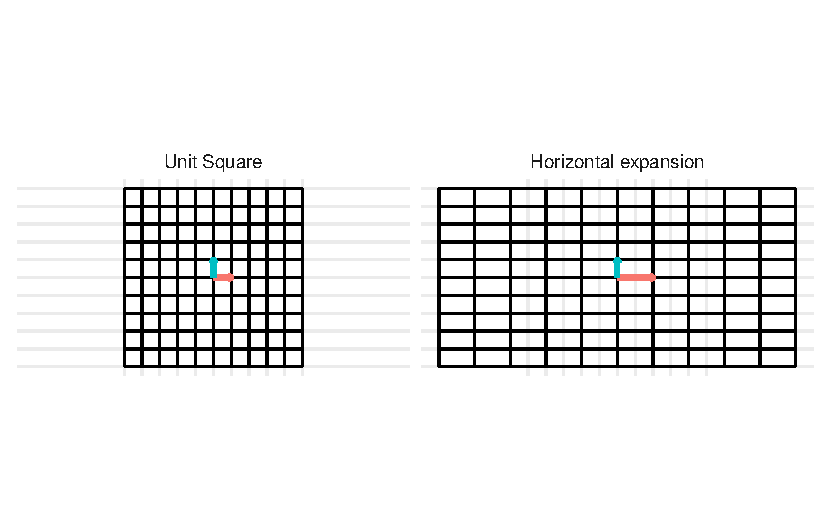
\includegraphics{multivariable-math_files/figure-latex/horizontal-expansion-static-1.pdf}

\hypertarget{horizonal-contraction}{%
\subsubsection{Horizonal Contraction}\label{horizonal-contraction}}

The matrix below gives a horizontal contraction when \(x < 1\)
* Horizontal contraction when \(x < 1\)

\[
\mathbf{A} = \begin{pmatrix}
x & 0 \\
0 & 1
\end{pmatrix}
\]

\begin{itemize}
\tightlist
\item
  In the example below, we set \(x = 0.5\)
\end{itemize}

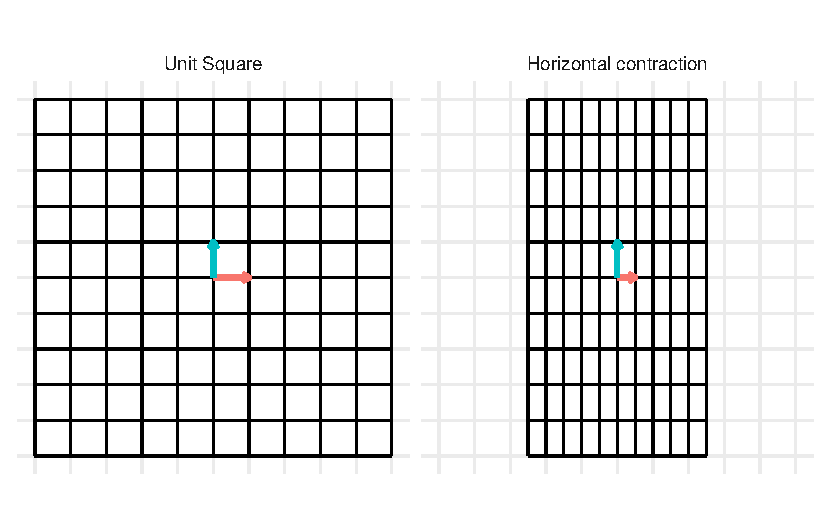
\includegraphics{multivariable-math_files/figure-latex/horizontal-contraction-static-1.pdf}

\hypertarget{vertical-expansion}{%
\subsubsection{Vertical Expansion}\label{vertical-expansion}}

The matrix below gives a vertical expansion when \(x > 1\)

\[
\mathbf{A} = \begin{pmatrix}
1 & 0 \\
0 & x
\end{pmatrix}
\]
* In the example below, we set \(x = 2\)

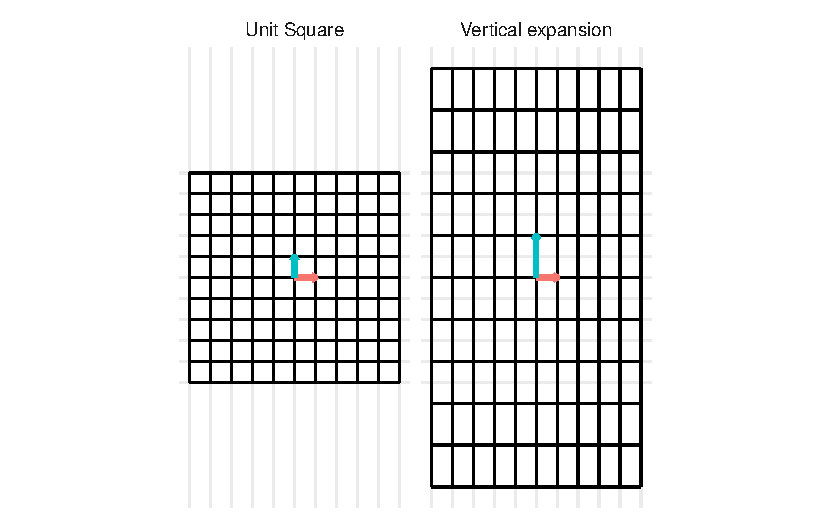
\includegraphics{multivariable-math_files/figure-latex/vertical-expansion-static-1.pdf}

\hypertarget{vertical-contraction}{%
\subsubsection{Vertical Contraction}\label{vertical-contraction}}

The matrix below gives a vertical contraction when \(x < 1\)

\[
\mathbf{A} = \begin{pmatrix}
1 & 0 \\
0 & x
\end{pmatrix}
\]

\begin{itemize}
\tightlist
\item
  In the example below, we set \(x = 0.5\)
\end{itemize}

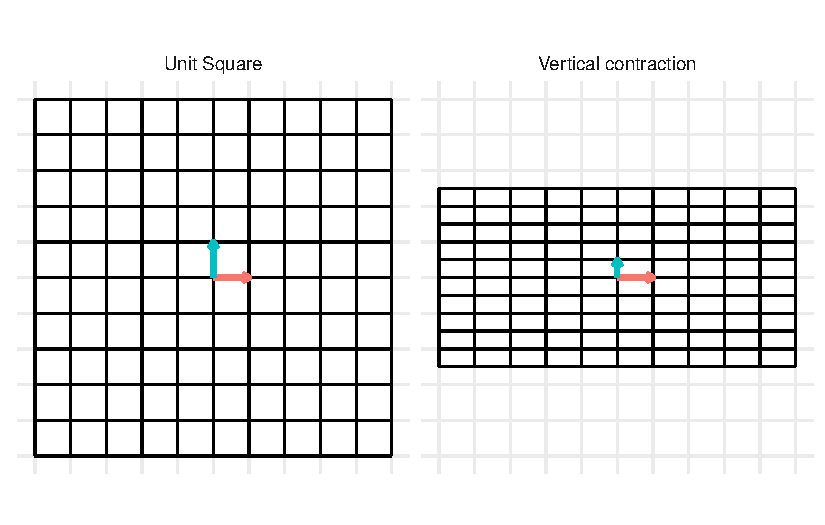
\includegraphics{multivariable-math_files/figure-latex/vertical-contraction-static-1.pdf}

\hypertarget{rotations}{%
\subsection{Rotations}\label{rotations}}

\hypertarget{rotation-by-90-degrees}{%
\subsubsection{Rotation by 90 degrees}\label{rotation-by-90-degrees}}

Rotations in 2D of an angle \(\theta \in [0, 2\pi]\) take the form of
\[
\mathbf{A} = \begin{pmatrix}
\cos(\theta) & -\sin(\theta) \\
\sin(\theta) & \cos(\theta)
\end{pmatrix}
\]
For example, a rotation of 90 degrees counter-clockwise (\(\theta = \frac{\pi}{2}\)) is given by the transformation matrix
\[
\mathbf{A} = \begin{pmatrix}
\cos(\frac{\pi}{2}) & -\sin(\frac{\pi}{2}) \\
\sin(\frac{\pi}{2}) & \cos(\frac{\pi}{2})
\end{pmatrix} = 
\begin{pmatrix}
0 & -1 \\
1 & 0
\end{pmatrix}
\]

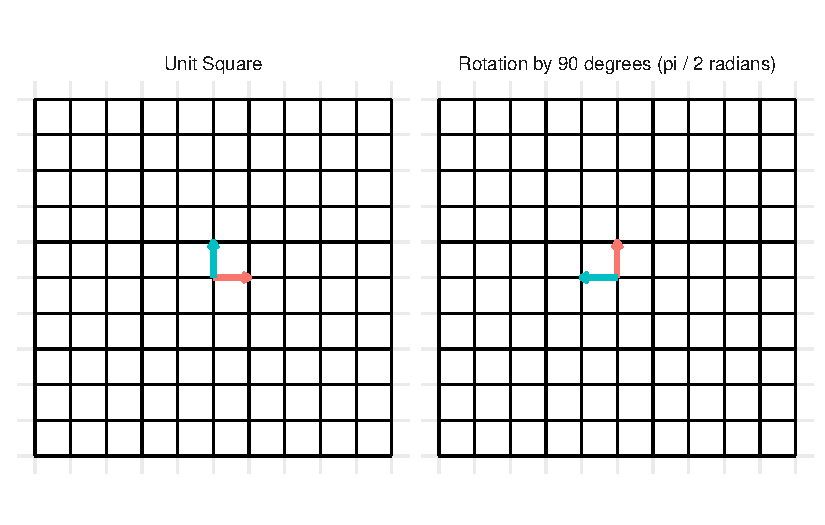
\includegraphics{multivariable-math_files/figure-latex/rotate-90-static-1.pdf}

Another example is for a rotation of 45 degrees clockwise (\(\theta = -\frac{\pi}{4}\)) is given by the transformation matrix
\[
 = \begin{pmatrix}
\cos(\frac{\pi}{4}) & -\sin(\frac{\pi}{4}) \\
\sin(\frac{\pi}{4}) & \cos(\frac{\pi}{4})
\end{pmatrix} = 
\begin{pmatrix}
\frac{\sqrt{2}}{2} & -\frac{\sqrt{2}}{2} \\
\frac{\sqrt{2}}{2} & \frac{\sqrt{2}}{2}
\end{pmatrix}
\]

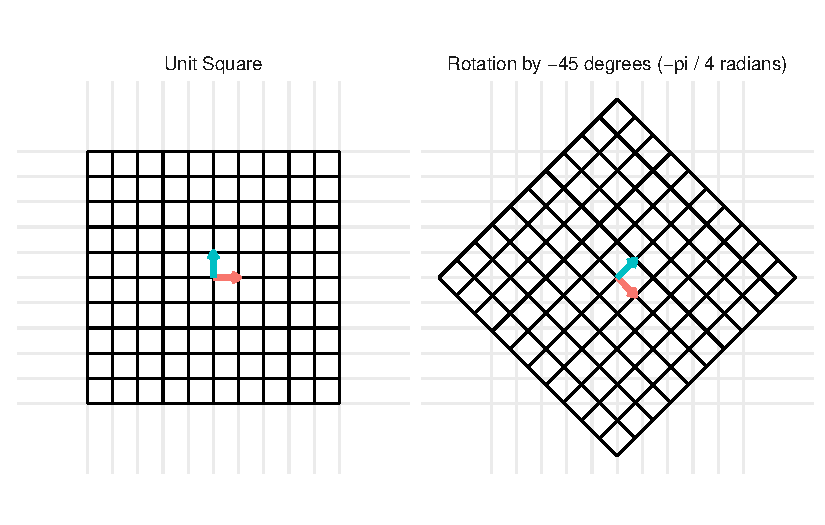
\includegraphics{multivariable-math_files/figure-latex/rotate-45-static-1.pdf}

\hypertarget{reflections}{%
\subsection{Reflections}\label{reflections}}

\hypertarget{reflection-across-the-x-axis}{%
\subsubsection{Reflection across the x-axis}\label{reflection-across-the-x-axis}}

The matrix below gives a reflection about the x-axis

\[
\mathbf{A} = \begin{pmatrix}
1 & 0 \\
0 & -1
\end{pmatrix}
\]

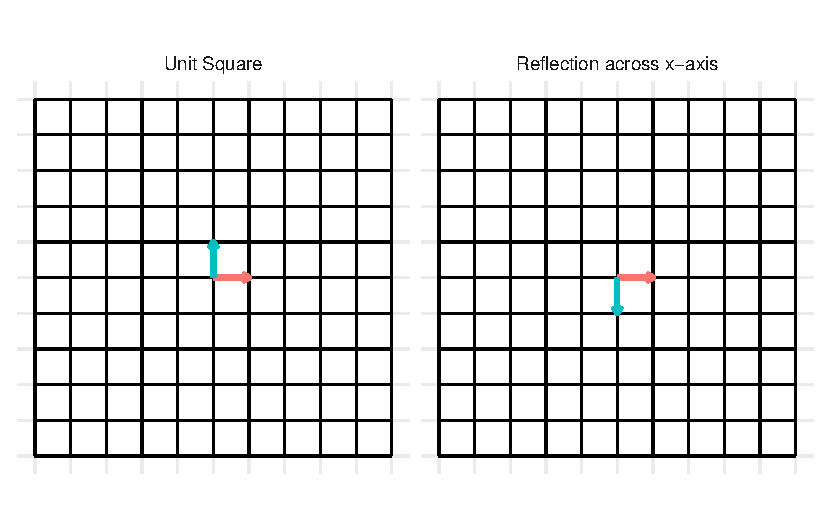
\includegraphics{multivariable-math_files/figure-latex/reflection-x-axis-1.pdf}

\hypertarget{reflection-across-the-y-axis}{%
\subsubsection{Reflection across the y-axis}\label{reflection-across-the-y-axis}}

The matrix below gives a reflection about the y-axis

\[
\mathbf{A} = \begin{pmatrix}
-1 & 0 \\
0 & 1
\end{pmatrix}
\]

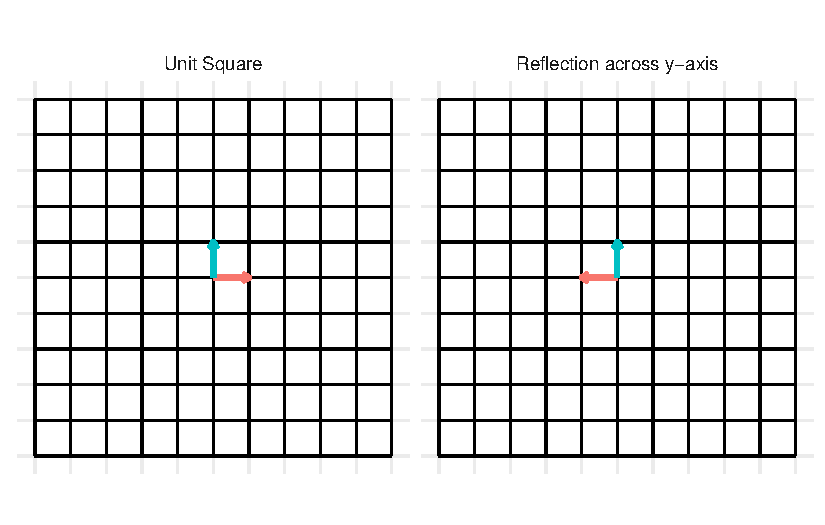
\includegraphics{multivariable-math_files/figure-latex/reflection-y-axis-static-1.pdf}

\hypertarget{reflection-across-the-line-y-x}{%
\subsubsection{Reflection across the line y = x}\label{reflection-across-the-line-y-x}}

\[
\mathbf{A} = \begin{pmatrix}
0 & 1 \\
1 & 0
\end{pmatrix}
\]

\begin{itemize}
\tightlist
\item
  In the example below, we set \(x = 0.5\)
\end{itemize}

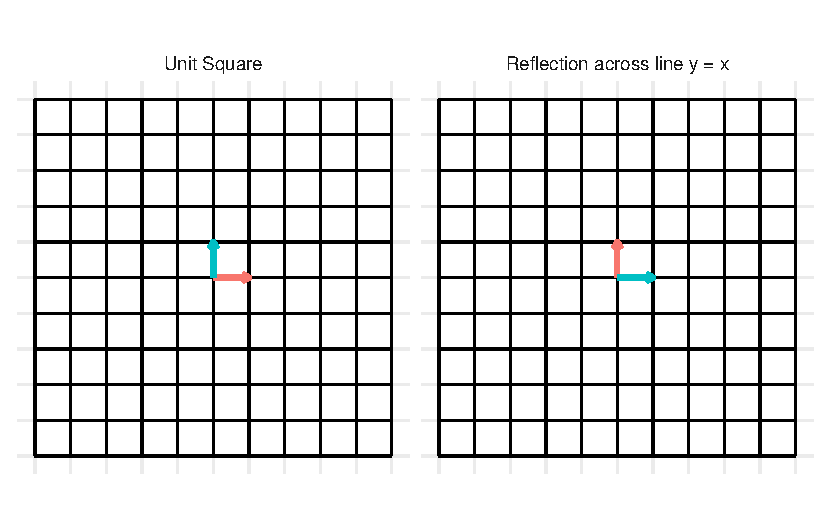
\includegraphics{multivariable-math_files/figure-latex/reflection-line-y-equals-x-static-1.pdf}

\hypertarget{reflection-across-the-line-y---x}{%
\subsubsection{Reflection across the line y = - x}\label{reflection-across-the-line-y---x}}

\[
\mathbf{A} = \begin{pmatrix}
0 & -1 \\
-1 & 0
\end{pmatrix}
\]

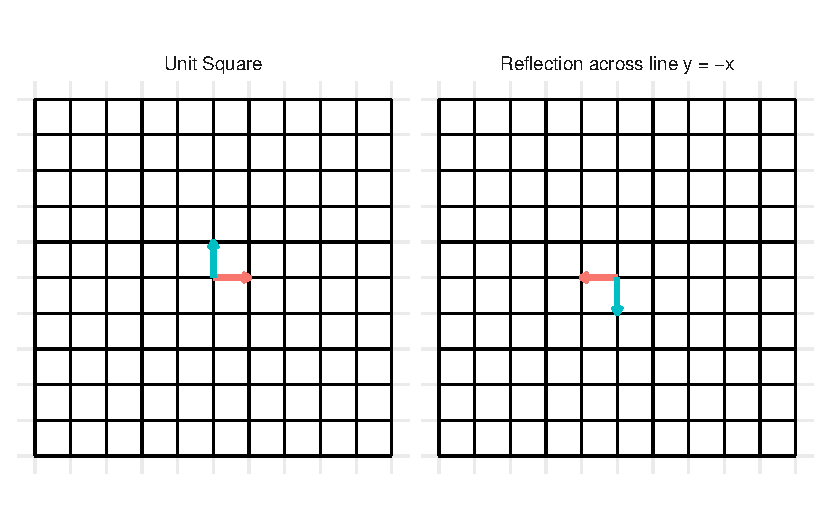
\includegraphics{multivariable-math_files/figure-latex/reflection-line-y-equals-minus-x-static-1.pdf}

\hypertarget{reflection-across-the-origin-0-0}{%
\subsubsection{Reflection across the origin (0, 0)}\label{reflection-across-the-origin-0-0}}

\[
\mathbf{A} = \begin{pmatrix}
-1 & 0 \\
0 & -1
\end{pmatrix}
\]

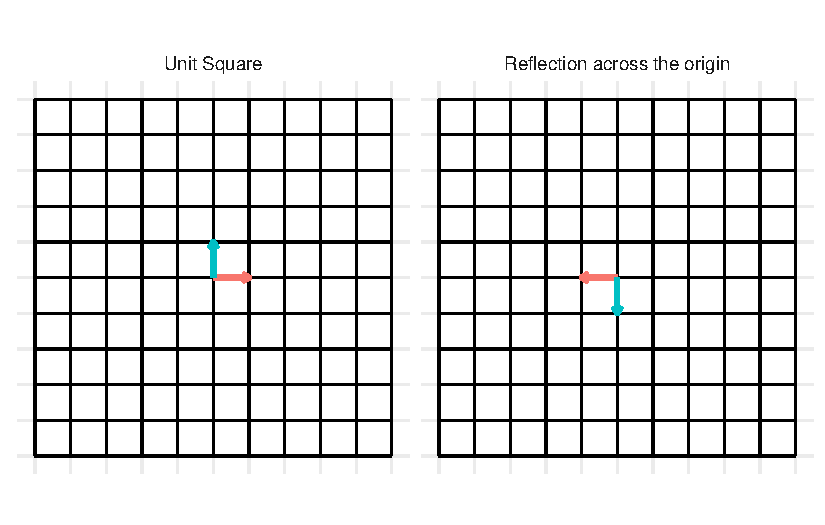
\includegraphics{multivariable-math_files/figure-latex/reflection-origin-static-1.pdf}

\hypertarget{shears}{%
\subsection{Shears}\label{shears}}

A shear transformation is like stretching play-dough if it was possible to stretch all parts of the dough uniformly (rather than some sections getting stretched more than others).

\hypertarget{horizontal-shear}{%
\subsubsection{Horizontal Shear}\label{horizontal-shear}}

\[
\mathbf{A} = \begin{pmatrix}
1 & x \\
0 & 1
\end{pmatrix}
\]
For the example below, we plot a horizontal shear with \(x = 2\).

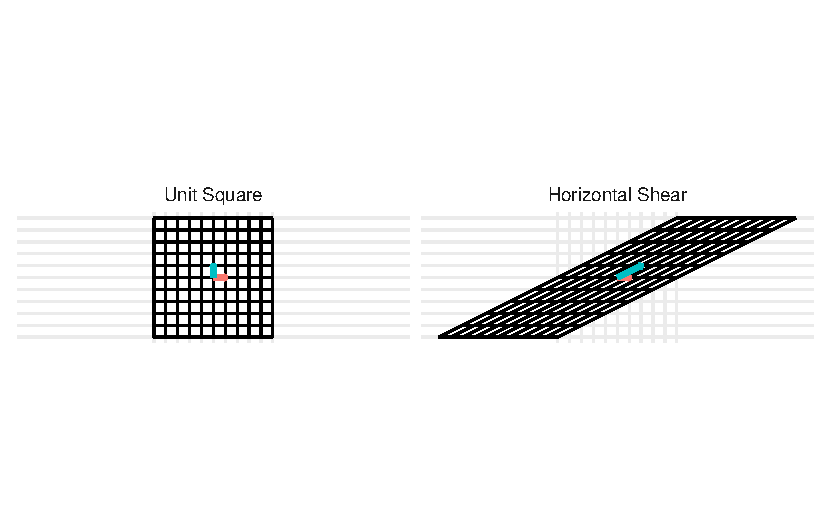
\includegraphics{multivariable-math_files/figure-latex/horizontal-shear-static-1.pdf}

\hypertarget{vertical-shear}{%
\subsubsection{Vertical Shear}\label{vertical-shear}}

\[
\mathbf{A} = \begin{pmatrix}
1 & 0 \\
x & 1
\end{pmatrix}
\]
For the example below, we plot a horizontal shear with \(x = 2\).

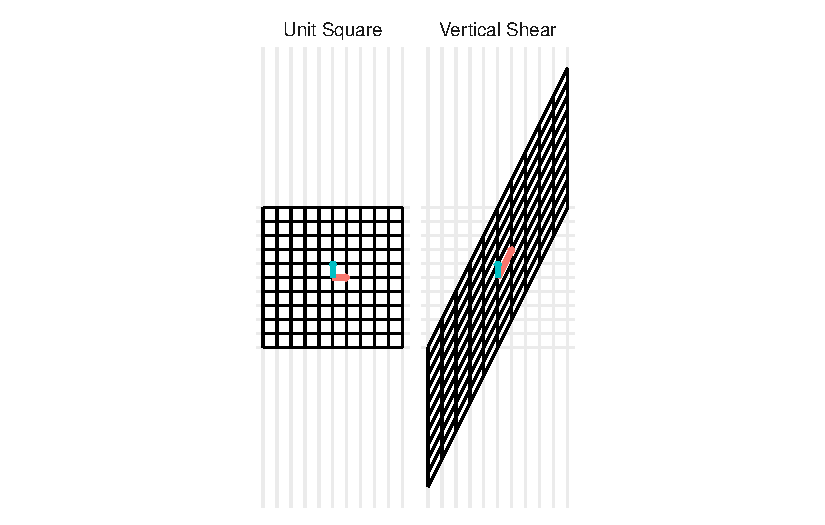
\includegraphics{multivariable-math_files/figure-latex/vertical-shear-static-1.pdf}

\hypertarget{projections}{%
\subsection{Projections}\label{projections}}

A projection is a mapping \(T:\mathcal{R}^n \rightarrow \mathcal{R}^n\) from one space (\(\mathbf{R}^n\)) to itself (\(\mathbf{R}^n\)) such that \(T^2 = T\)

\hypertarget{project-onto-the-x-axis}{%
\subsubsection{Project onto the x-axis}\label{project-onto-the-x-axis}}

\[
\mathbf{A} = \begin{pmatrix}
1 & 0 \\
0 & 0
\end{pmatrix}
\]
For the example below, we plot a projection onto the x-axis

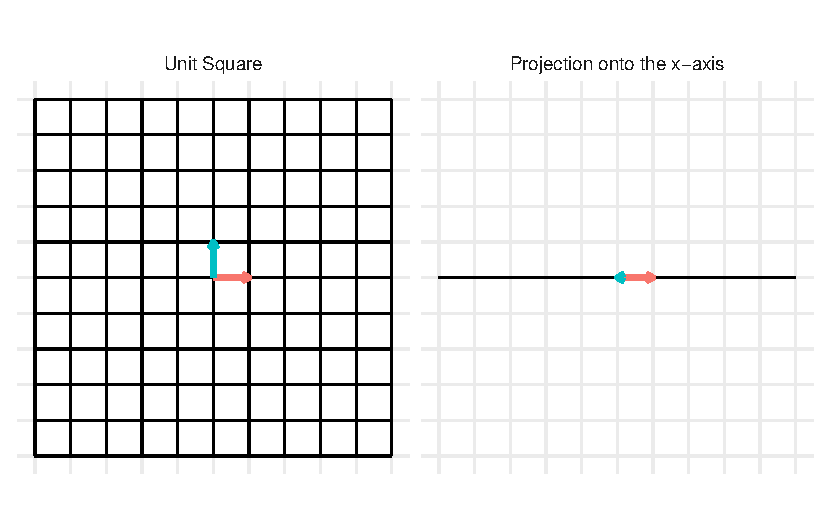
\includegraphics{multivariable-math_files/figure-latex/projection-x-static-1.pdf}

\hypertarget{project-onto-the-y-axis}{%
\subsubsection{Project onto the y-axis}\label{project-onto-the-y-axis}}

\[
\mathbf{A} = \begin{pmatrix}
0 & 0 \\
0 & 1
\end{pmatrix}
\]
For the example below, we plot a projection onto the y-axis

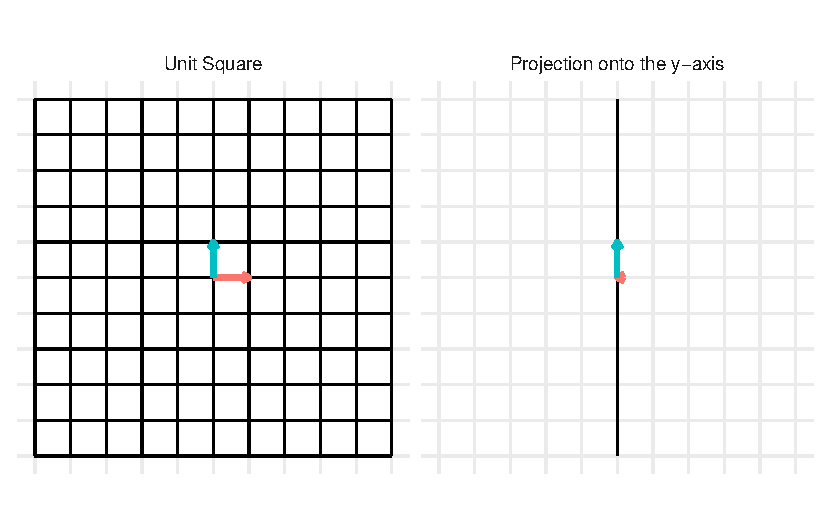
\includegraphics{multivariable-math_files/figure-latex/projection-y-static-1.pdf}

\hypertarget{identity}{%
\subsection{Identity}\label{identity}}

The identity transformation is the transformation that leaves the vector input unchanged. The identity matrix is typically written as \(\mathbf{I}\)

\[
\mathbf{I} = \begin{pmatrix}
1 & 0 \\
0 & 1
\end{pmatrix}
\]

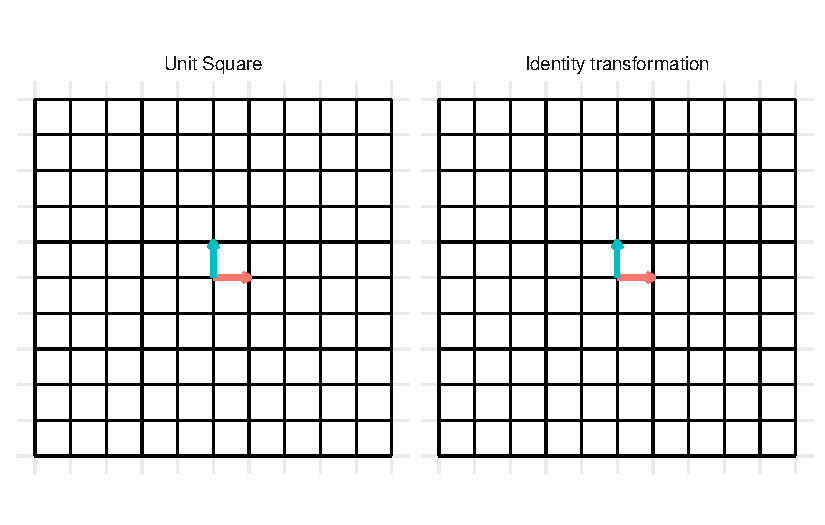
\includegraphics{multivariable-math_files/figure-latex/identity-static-1.pdf}

\hypertarget{properties-of-matrix-transformations}{%
\section{Properties of matrix transformations}\label{properties-of-matrix-transformations}}

\hypertarget{one-to-one-transformations}{%
\subsection{One-to-one transformations}\label{one-to-one-transformations}}

\begin{definition}
A transformation \(T:\mathcal{R}^n \rightarrow \mathcal{R}^m\) is called \textbf{one-to-one} if every vector \(\mathbf{b}\) in the image \(\mathcal{R}^m\), the equation \(T(\mathbf{x}) = \mathbf{b}\) has \textbf{at most} one solution in \(\mathcal{R}^n\).
\end{definition}

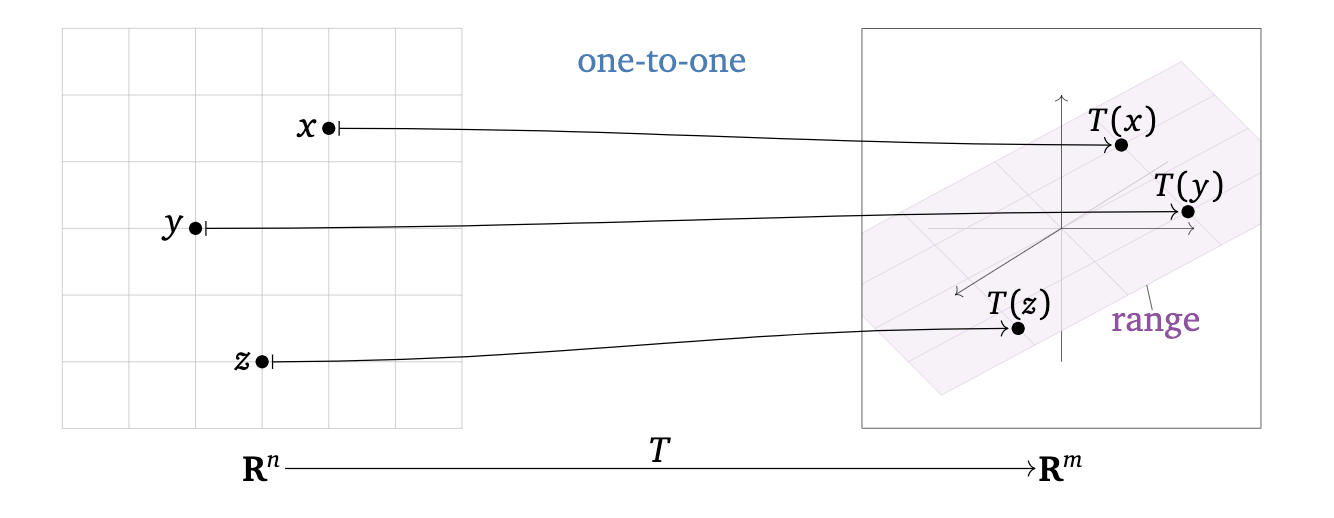
\includegraphics[width=1\linewidth]{images/one-to-one}

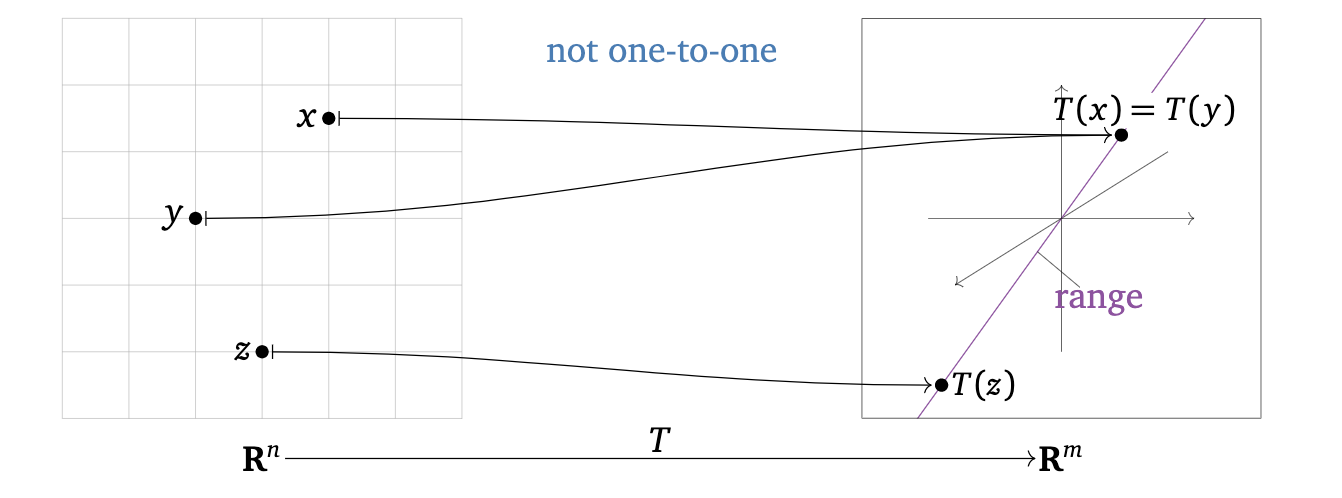
\includegraphics[width=1\linewidth]{images/not-one-to-one}

The following statements are equivalent was of saying \(T:\mathcal{R}^n \rightarrow \mathcal{R}^m\) is one-to-one:

\begin{enumerate}
\def\labelenumi{\alph{enumi})}
\item
  For every \(\mathbf{b} \in \mathcal{R}^m\) (for every vector in the image), the equation \(T(\mathbf{x}) = \mathbf{b}\) has either zero or one solution
\item
  Every different input into the function \(T(\cdot)\) has a different output
\item
  If \(T(\mathbf{u}) = T(\mathbf{v})\) then \(\mathbf{u} = \mathbf{v}\)
\end{enumerate}

The following statements are equivalent was of saying \(T:\mathcal{R}^n \rightarrow \mathcal{R}^m\) is \textbf{not} one-to-one:

\begin{enumerate}
\def\labelenumi{\alph{enumi})}
\item
  There exists as least one \(\mathbf{b} \in \mathcal{R}^m\) such that the equation \(T(\mathbf{x}) = \mathbf{b}\) has more than one solution
\item
  There are at least two different inputs into the function \(T(\cdot)\) that have the same output
\item
  There exist vectors \(\mathbf{u} \neq \mathbf{v} \in \mathcal{R}^n\) such that \(T(\mathbf{u}) = T(\mathbf{v})\)
\end{enumerate}

\begin{theorem}

Let \(\mathbf{A}\mathbf{x}\) be the matrix representation of the linear transformation \(T(\mathbf{x})\) for the \(m \times n\) matrix \(\mathbf{A}\). Then the following statements are equivalent:

\begin{enumerate}
\def\labelenumi{\arabic{enumi})}
\item
  \(T\) is one-to-one.
\item
  For every \(\mathbf{b} \in \mathcal{R}^m\), the equation \(T(\mathbf{x}) = \mathbf{b}\) has at most one solution.
\item
  For every \(\mathbf{b} \in \mathcal{R}^m\), the equation \(\mathbf{A}\mathbf{x} = \mathbf{b}\) has a unique solution or is inconsistent.
\item
  The equation \(\mathbf{A}\mathbf{x} = \mathbf{0}\) has only a trivial solution.
\item
  The columns of \(\mathbf{A}\) are linearly independent.
\item
  \(\mathbf{A}\) has a pivot in every column.
\item
  The range of \(\mathbf{A}\) has dimension \(n\)
\end{enumerate}

\end{theorem}

\begin{itemize}
\tightlist
\item
  \textbf{Example:} is the following matrix one-to-one?
\end{itemize}

\[
\mathbf{A} = \begin{pmatrix}
1 & 0 \\
0 & 1 \\
1 & 1
\end{pmatrix}
\]

\begin{itemize}
\tightlist
\item
  \textbf{Example:} is the following matrix one-to-one?
\end{itemize}

\[
\mathbf{A} = \begin{pmatrix}
1 & 0 & 0 \\
0 & 1 & 0 \\
1 & 1 & 0
\end{pmatrix}
\]

\textbf{Note:} Matrices that are wider than they are tall are not one-to-one transformations. (This does not mean that all tall matrices are one-to-one)

\hypertarget{onto-transformations}{%
\subsection{Onto transformations}\label{onto-transformations}}

\begin{definition}
A transformation \(T:\mathcal{R}^n \rightarrow \mathcal{R}^m\) is called \textbf{onto} if, for every vector \(\mathbf{b} \in \mathcal{R}^m\), the equation \(T(\mathbf{x}) = \mathbf{b}\) has \textbf{at least} one solution \(\mathbf{x} \in \mathcal{R}^n\)
\end{definition}

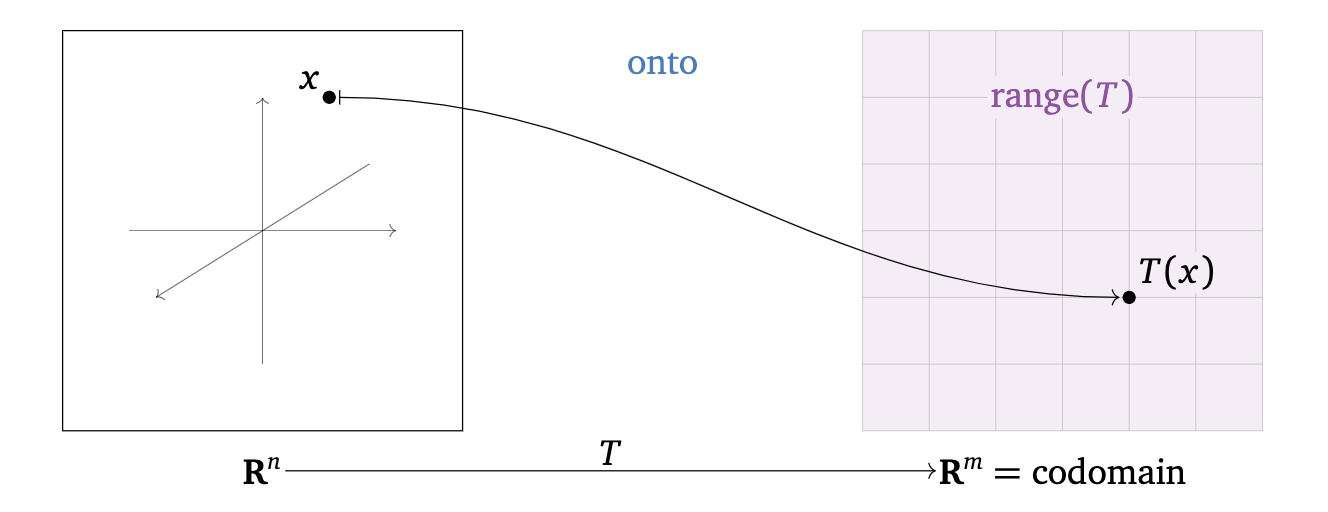
\includegraphics[width=1\linewidth]{images/onto}

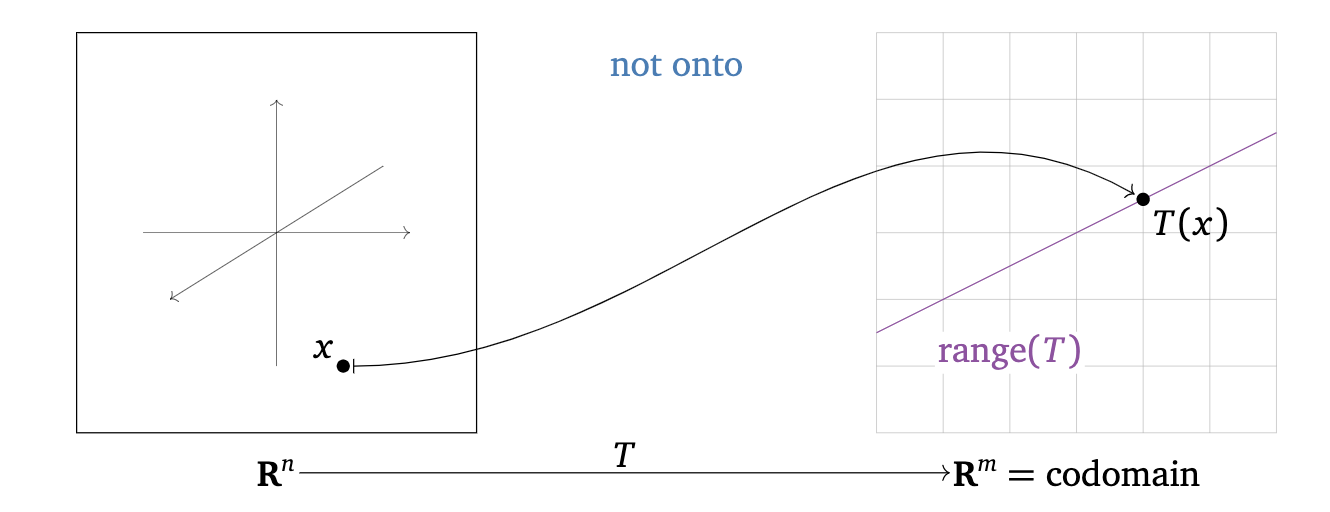
\includegraphics[width=1\linewidth]{images/not-onto}

The following are equivalent ways of saying that \(T:\mathcal{R}^n \rightarrow \mathcal{R}^m\) is onto:

\begin{enumerate}
\def\labelenumi{\arabic{enumi})}
\item
  The range of \(T:\mathcal{R}^n \rightarrow \mathcal{R}^m\) is equal to the codomain of \(T:\mathcal{R}^n \rightarrow \mathcal{R}^m\)
\item
  Every vector in the codomain is the output of some input vector
\end{enumerate}

The following are equivalent ways of saying that \(T:\mathcal{R}^n \rightarrow \mathcal{R}^m\) is not onto:

\begin{enumerate}
\def\labelenumi{\arabic{enumi})}
\item
  The range of \(T:\mathcal{R}^n \rightarrow \mathcal{R}^m\) is smaller than the codomain of \(T:\mathcal{R}^n \rightarrow \mathcal{R}^m\).
\item
  There exists a vector \(\mathbf{b} \in \mathcal{R}^m\) such that the equation \(T(\mathbf{x})\) does not have a solution.
\item
  There is a vector in the codomain that is not the output of any input vector.
\end{enumerate}

\begin{theorem}

Let \(\mathbf{A}\mathbf{x}\) be the matrix representation of the linear transformation \(T(\mathbf{x})\) for the \(m \times n\) matrix \(\mathbf{A}\). Then the following statements are equivalent:

\begin{enumerate}
\def\labelenumi{\arabic{enumi})}
\item
  \(T\) is onto
\item
  \(T(\mathbf{x}) = \mathbf{b}\) has at least one solution for every \(\mathbf{b} \in \mathcal{R}^m\).
\item
  The equation \(\mathbf{A}\mathbf{x} = \mathbf{b}\) is consistent for every \(\mathbf{b} \in \mathcal{R}^m\).
\item
  The columns of \(\mathbf{A}\) span \(\mathcal{R}^m\)
\item
  \(\mathbf{A}\) has a pivot in every row
\item
  The range of \(T:\mathcal{R}^n \rightarrow \mathcal{R}^m\) has dimension \(m\)
\end{enumerate}

\end{theorem}

\begin{itemize}
\item
  \textbf{Example:}
\item
  \textbf{Example:} is the following matrix onto?
\end{itemize}

\[
\mathbf{A} = \begin{pmatrix}
1 & 1 & 0 \\
0 & 1 & 1
\end{pmatrix}
\]

\begin{itemize}
\tightlist
\item
  \textbf{Example:} is the following matrix one-to-one?
\end{itemize}

\[
\mathbf{A} = \begin{pmatrix}
1 & 0  \\
0 & 1  \\
1 & 0
\end{pmatrix}
\]

\textbf{Note:} Matrices that are taller than they are wide are not onto transformations. (This does not mean that all wide matrices are onto)

\hypertarget{matrix-operations}{%
\chapter{Matrix operations}\label{matrix-operations}}

\hypertarget{todo}{%
\section{ToDo}\label{todo}}

\begin{itemize}
\item
  define dot product here
\item
  Show matrix multiplication using dot products
\item
  move to chapter 1 or 2
\item
  \href{https://www.3blue1brown.com/lessons/matrix-multiplication}{3 Blue 1 Brown -- Matrix Multiplication}
\item
  \textbf{Note: add examples:}
\end{itemize}

\hypertarget{properties-of-matrices}{%
\section{Properties of matrices}\label{properties-of-matrices}}

\hypertarget{matrix-addition}{%
\subsection{Matrix Addition}\label{matrix-addition}}

\textbf{Matrix Addition:} If the matrices \(\mathbf{A}\) and \(\mathbf{B}\) are of the same dimension (e.g., both \(\mathbf{A}\) and \(\mathbf{B}\) have the same number of rows \(m\) and the same number of columns \(n\)), then

\[
\begin{aligned}
\mathbf{A} + \mathbf{B} & = \begin{pmatrix} a_{11} & a_{12} & \cdots & a_{1n} \\
a_{21} & a_{22} & \cdots & a_{2n} \\
\vdots & \vdots & \ddots & \vdots \\
a_{m1} & a_{m2} & \cdots & a_{mn}
\end{pmatrix} + 
\begin{pmatrix} b_{11} & b_{12} & \cdots & b_{1n} \\
b_{21} & b_{22} & \cdots & b_{2n} \\
\vdots & \vdots & \ddots & \vdots \\
b_{m1} & b_{m2} & \cdots & b_{mn}
\end{pmatrix} \\
& = \begin{pmatrix} a_{11} + b_{11} & b_{12} + b_{12} & \cdots & a_{1n} + b_{1n} \\
a_{21} + b_{21} & a_{22} + b_{22} & \cdots & a_{2n} + b_{2n} \\
\vdots & \vdots & \ddots & \vdots \\
a_{m1} + b_{m1} & a_{m2} + b_{m2} & \cdots & a_{mn} + b_{mn}
\end{pmatrix} \\
& = \left\{ a_{ij} + b_{ij} \right\}
\end{aligned}
\label{eq:matrix-addition}
\]

\textbf{\ldots{} Another way to }

If \(\mathbf{A}\) and \(\mathbf{B}\) are of the same dimension (same number of rows and columns) you can add the matrices together

\begin{Shaded}
\begin{Highlighting}[]
\NormalTok{A <-}\StringTok{ }\KeywordTok{matrix}\NormalTok{(}\KeywordTok{c}\NormalTok{(}\DecValTok{4}\NormalTok{, }\DecValTok{1}\NormalTok{, }\DecValTok{33}\NormalTok{, }\DecValTok{2}\NormalTok{, }\DecValTok{0}\NormalTok{, }\DecValTok{-4}\NormalTok{), }\DecValTok{3}\NormalTok{, }\DecValTok{2}\NormalTok{)}
\NormalTok{B <-}\StringTok{ }\KeywordTok{matrix}\NormalTok{(}\KeywordTok{c}\NormalTok{(}\DecValTok{7}\NormalTok{, }\DecValTok{-24}\NormalTok{, }\DecValTok{3}\NormalTok{, }\DecValTok{9}\NormalTok{, }\DecValTok{11}\NormalTok{, }\DecValTok{-9}\NormalTok{), }\DecValTok{3}\NormalTok{, }\DecValTok{2}\NormalTok{)}
\NormalTok{A}
\end{Highlighting}
\end{Shaded}

\begin{verbatim}
##      [,1] [,2]
## [1,]    4    2
## [2,]    1    0
## [3,]   33   -4
\end{verbatim}

\begin{Shaded}
\begin{Highlighting}[]
\NormalTok{B}
\end{Highlighting}
\end{Shaded}

\begin{verbatim}
##      [,1] [,2]
## [1,]    7    9
## [2,]  -24   11
## [3,]    3   -9
\end{verbatim}

\begin{Shaded}
\begin{Highlighting}[]
\NormalTok{A }\OperatorTok{+}\StringTok{ }\NormalTok{B}
\end{Highlighting}
\end{Shaded}

\begin{verbatim}
##      [,1] [,2]
## [1,]   11   11
## [2,]  -23   11
## [3,]   36  -13
\end{verbatim}

We can also write this using \texttt{for} loops

\begin{Shaded}
\begin{Highlighting}[]
\CommentTok{# initialize an empty matrix to fill}
\NormalTok{C <-}\StringTok{ }\KeywordTok{matrix}\NormalTok{(}\DecValTok{0}\NormalTok{, }\DecValTok{3}\NormalTok{, }\DecValTok{2}\NormalTok{)}

\ControlFlowTok{for}\NormalTok{ (i }\ControlFlowTok{in} \DecValTok{1}\OperatorTok{:}\KeywordTok{nrow}\NormalTok{(A)) \{         }\CommentTok{# loop over the rows}
    \ControlFlowTok{for}\NormalTok{ (j }\ControlFlowTok{in} \DecValTok{1}\OperatorTok{:}\KeywordTok{ncol}\NormalTok{(A)) \{     }\CommentTok{# loop over the columns}
\NormalTok{        C[i, j] <-}\StringTok{ }\NormalTok{A[i, j] }\OperatorTok{+}\StringTok{ }\NormalTok{B[i, j]}
\NormalTok{    \}}
\NormalTok{\}}
\NormalTok{C}
\end{Highlighting}
\end{Shaded}

\begin{verbatim}
##      [,1] [,2]
## [1,]   11   11
## [2,]  -23   11
## [3,]   36  -13
\end{verbatim}

If \(\mathbf{A}\) and \(\mathbf{B}\) are of different dimensions (they differ in either the number of rows or columns), \texttt{R} will return an error warning you that the matrices are of different sizes and can't be added

\begin{Shaded}
\begin{Highlighting}[]
\NormalTok{A <-}\StringTok{ }\KeywordTok{matrix}\NormalTok{(}\KeywordTok{c}\NormalTok{(}\DecValTok{4}\NormalTok{, }\DecValTok{1}\NormalTok{, }\DecValTok{33}\NormalTok{, }\DecValTok{2}\NormalTok{, }\DecValTok{0}\NormalTok{, }\DecValTok{-4}\NormalTok{), }\DecValTok{3}\NormalTok{, }\DecValTok{2}\NormalTok{)}
\NormalTok{B <-}\StringTok{ }\KeywordTok{matrix}\NormalTok{(}\KeywordTok{c}\NormalTok{(}\DecValTok{7}\NormalTok{, }\DecValTok{-24}\NormalTok{, }\DecValTok{3}\NormalTok{, }\DecValTok{9}\NormalTok{), }\DecValTok{2}\NormalTok{, }\DecValTok{2}\NormalTok{)}
\NormalTok{A}
\end{Highlighting}
\end{Shaded}

\begin{verbatim}
##      [,1] [,2]
## [1,]    4    2
## [2,]    1    0
## [3,]   33   -4
\end{verbatim}

\begin{Shaded}
\begin{Highlighting}[]
\NormalTok{B}
\end{Highlighting}
\end{Shaded}

\begin{verbatim}
##      [,1] [,2]
## [1,]    7    3
## [2,]  -24    9
\end{verbatim}

\begin{Shaded}
\begin{Highlighting}[]
\NormalTok{A }\OperatorTok{+}\StringTok{ }\NormalTok{B}
\end{Highlighting}
\end{Shaded}

\begin{verbatim}
## Error in A + B: non-conformable arrays
\end{verbatim}

\begin{theorem}

Let \(\mathbf{A}\), \(\mathbf{B}\), and \(\mathbf{C}\) be \(m \times n\) matrices and let \(a\) and \(b\) be scalars, then:

\begin{enumerate}
\def\labelenumi{\arabic{enumi})}
\item
  \(\mathbf{A} + \mathbf{B} = \mathbf{B} + \mathbf{A}\) \hfill [(commutivity of addition)]{style="float:right"}
\item
  \((\mathbf{A} + \mathbf{B}) + \mathbf{C} = \mathbf{A} + (\mathbf{B} + \mathbf{C})\) \hfill [(commutivity of addition)]{style="float:right"}
\item
  \(\mathbf{A} + \mathbf{0} = \mathbf{A}\) \hfill [(additive identity)]{style="float:right"}
\item
  \(a (\mathbf{A} + \mathbf{B}) = a \mathbf{A} + a \mathbf{B}\) \hfill [(scalar ...)]{style="float:right"}
\item
  \((a + b)\mathbf{A} = a \mathbf{A} + b \mathbf{A}\) \hfill [(scalar ...)]{style="float:right"}
\item
  \((ab)\mathbf{A} = a (b\mathbf{A})\) \hfill [(scalar ...)]{style="float:right"}
\end{enumerate}

\end{theorem}

\hypertarget{matrix-multipliation}{%
\subsection{Matrix Multipliation}\label{matrix-multipliation}}

\textbf{Matrix Multiplication:} If \(\mathbf{A} = \left\{ a_{ij} \right\}\) is an \(m \times n\) matrix and \(\mathbf{B} = \left\{ a_{jk} \right\}\) is a \(n \times p\) matrix, then the matrix product \(\mathbf{C} = \mathbf{A} \mathbf{B}\) is an \(m \times p\) matrix where \(\mathbf{C} = \left\{ \sum_{j=1}^p a_{ij} b{jk} \right\}\)

\[
\begin{aligned}
\mathbf{A} \mathbf{B} & = \begin{pmatrix} a_{11} & a_{12} & \cdots & a_{1n} \\
a_{21} & a_{22} & \cdots & a_{2n} \\
\vdots & \vdots & \ddots & \vdots \\
a_{m1} & a_{m2} & \cdots & a_{mn}
\end{pmatrix} 
\begin{pmatrix} b_{11} & b_{12} & \cdots & b_{1p} \\
b_{21} & b_{22} & \cdots & b_{2p} \\
\vdots & \vdots & \ddots & \vdots \\
b_{n1} & b_{n2} & \cdots & b_{np}
\end{pmatrix} \\
& = \begin{pmatrix} \sum_{j=1}^n a_{1j} b_{j1} & \sum_{j=1}^n a_{1j} b_{j2} & \cdots & \sum_{j=1}^n a_{1j} b_{jp} \\
\sum_{j=1}^n a_{2j} b_{j1} &\sum_{j=1}^n a_{2j} b_{j2} & \cdots & \sum_{j=1}^n a_{2j} b_{jp} \\
\vdots & \vdots & \ddots & \vdots \\
\sum_{j=1}^n a_{mj} b_{j1} &\sum_{j=1}^n a_{nj} b_{j2} & \cdots & \sum_{j=1}^n a_{mj} b_{jp}
\end{pmatrix} 
\end{aligned}
\label{eq:matrix-multiplication}
\]

Another way to define matrix multiplication is through inner product notation. Define the \(m \times n\) matrix \(\mathbf{A}\) and the \(n \times p\) matrix \(\mathbf{B}\) as the partition

\[
\begin{aligned}
\mathbf{A} & = \begin{pmatrix} \mathbf{a}_{1}' \\
\mathbf{a}_{2}' \\ 
\vdots \\
\mathbf{a}_{m}' \end{pmatrix}
& \mbox{ and } 
&& \mathbf{B} & = \begin{pmatrix} \mathbf{b}_{1} & \mathbf{b}_{2} & \cdots & \mathbf{b}_{p} \end{pmatrix} 
\end{aligned}
\]

where \(\mathbf{a}_i\) and \(\mathbf{b}_k\) are both \(n\)-vectors. Then, we have \(\mathbf{C} = \mathbf{A} \mathbf{B}\) can be written as

\[
\begin{aligned}
\mathbf{A} \mathbf{B}  = \mathbf{A} \begin{pmatrix} \mathbf{b}_1 & \mathbf{b}_2 & \cdots & \mathbf{b}_p
\end{pmatrix}  = \begin{pmatrix} \mathbf{A} \mathbf{b}_1 & \mathbf{A} \mathbf{b}_2 & \cdots & \mathbf{A} \mathbf{b}_p
\end{pmatrix} 
\end{aligned}
\]

Note that in this representation, each column of the matrix \(\mathbf{A}\mathbf{B}\) is a linear combination the the columns of \(\mathbf{A}\) with coefficients given by the corresponding column of \(\mathbf{B}\).

\[
\begin{aligned}
\mathbf{A} \mathbf{B} & = \begin{pmatrix} \mathbf{a}_1' \mathbf{b}_1 & \mathbf{a}_1' \mathbf{b}_2 & \cdots & \mathbf{a}_1' \mathbf{b}_q \\
\mathbf{a}_2' \mathbf{b}_1 & \mathbf{a}_2' \mathbf{b}_2 & \cdots & \mathbf{a}_2' \mathbf{b}_q \\
\vdots & \vdots & \ddots & \vdots \\
\mathbf{a}_n' \mathbf{b}_1 & \mathbf{a}_n' \mathbf{b}_2  & \cdots & \mathbf{a}_n' \mathbf{b}_q
\end{pmatrix} \\
& = \left\{ \mathbf{a}_i' \mathbf{b}_k  \right\}.
\end{aligned}
\]

Written in this notation, we arrive at the multiplication rule for \(\mathbf{C} = \mathbf{A} \mathbf{B}\) -- the \(ik\)th element \(c_{ik}\) of \(\mathbf{C}\) is the inner product of the \(i\)th row of \(\mathbf{A}\) and the \(j\)th column of \(\mathbf{B}\).

\hypertarget{properties-of-matrix-multiplication}{%
\subsection{Properties of Matrix Multiplication}\label{properties-of-matrix-multiplication}}

Define the \(m \times m\) \textbf{identity matrix} \(\mathbf{I}_m\) with ones on the diagonal and zeros off diagonal as
\[
\mathbf{I}_m = \begin{pmatrix} 1 & 0 & \cdots & 0 \\ 0 & 1 & \cdots & 0 \\ 0 & 0 & \ddots & 0 \\ 0 & 0 & \cdots & 1\end{pmatrix}
\]
Let \(\mathbf{A}\) be an \(m \times n\) matrix, then:

\begin{enumerate}
\def\labelenumi{\arabic{enumi})}
\item
  Let \(\mathbf{B}\) be an \(n \times p\) matrix and \(\mathbf{C}\) a \(p \times q\) matrix. Then \(\mathbf{A}(\mathbf{B}\mathbf{C}) = (\mathbf{A}\mathbf{B})\mathbf{C}\) is an \(m \times q\) matrix.
\item
  Let \(\mathbf{B}\) and \(\mathbf{C}\) be \(n \times p\) matrices. Then \(\mathbf{A}(\mathbf{B} + \mathbf{C}) = \mathbf{A}\mathbf{B} + \mathbf{A}\mathbf{C}\) is an \(m \times p\) matrix.
\item
  Let \(\mathbf{B}\) and \(\mathbf{C}\) be \(p \times m\) matrices. Then \((\mathbf{B} + \mathbf{C})\mathbf{A} = \mathbf{B}\mathbf{A} + \mathbf{C}\mathbf{A}\) is an \(p \times m\) matrix.
\item
  Let \(\mathbf{B}\) be an \(p \times m\) matrix and \(c\) a scalar. Then \(c(\mathbf{A} \mathbf{B}) = (c \mathbf{A}) \mathbf{B} = \mathbf{A}(c\mathbf{B})\) is an \(p \times m\) matrix.
\item
  \(\mathbf{I}_m \mathbf{A} = \mathbf{A} \mathbf{I}_n = \mathbf{A}\)
\end{enumerate}

\textbf{Examples: in class}

\textbf{Note:} Matrix multiplication violates some of the rules of multiplication that you might be used to. Pay attention for the following:

\begin{enumerate}
\def\labelenumi{\arabic{enumi})}
\item
  In general \(\mathbf{A} \mathbf{B} \neq \mathbf{B} \mathbf{A}\) (sometimes these are equal, but usually are not)
\item
  \(\mathbf{A}\mathbf{B} = \mathbf{A} \mathbf{C}\) \textbf{does not} imply \(\mathbf{B} = \mathbf{C}\)
\item
  \(\mathbf{A}\mathbf{B} = \mathbf{0}\) does not imply that \(\mathbf{A} = \mathbf{0}\) or \(\mathbf{B} = \mathbf{0}\)
\end{enumerate}

\hypertarget{matrix-multiplication-complexity-big-o-notation}{%
\subsection{Matrix Multiplication complexity (Big O notation)}\label{matrix-multiplication-complexity-big-o-notation}}

In the study of algorithms, the notation \(O(n)\) is used to describe the number of calculations that need to be done to evaluate the equation. As an example, consider \(\mathbf{A} = \begin{pmatrix}3 & 1 \\ 2 & -3 \end{pmatrix}\), \(\mathbf{B} = \begin{pmatrix} -2 & 4 \\ -1 & 2 \end{pmatrix}\), and \(\mathbf{x} = \begin{pmatrix} -3 \\ 1 \end{pmatrix}\).

\textbf{By hand:} Calculate

\begin{enumerate}
\def\labelenumi{\arabic{enumi})}
\item
  \((\mathbf{A} \mathbf{B}) \mathbf{x}\)
\item
  \(\mathbf{A} (\mathbf{B} \mathbf{x})\)
\end{enumerate}

Which was easier? Which required less calculation?

\begin{itemize}
\item
  Matrix-matrix multiplication of and \(m \times n\) matrix \(\mathbf{A}\) and an \(m \times p\) matrix \(\mathbf{B}\) has complexity \(O(m n p)\).
\item
  Matrix-vector multiplication of and \(m \times n\) matrix \(\mathbf{A}\) and an \(p\)-vector \(\mathbf{x}\) has complexity \(O(n m)\).
\end{itemize}

From example above:

\begin{enumerate}
\def\labelenumi{\arabic{enumi})}
\item
  \(O(m n p)\) matrix-matrix multiplication \((\mathbf{A} \mathbf{B})\) followed by \(O(m n)\) matrix-vector multiplication \((\mathbf{A} \mathbf{B}) \mathbf{x}\) which has computational complexity \(O(m n p) + O(m n)\)
\item
  \(O(m n)\) matrix-vector multiplication \((\mathbf{B} \mathbf{x})\) followed by \(O(m n)\) matrix-vector multiplication \(\mathbf{A} (\mathbf{B} \mathbf{x})\) which has computational complexity \(O(m n) + O(m n)\)
\end{enumerate}

\hypertarget{matrix-powers}{%
\subsection{Matrix powers}\label{matrix-powers}}

Powers of a \(n \times n\) (square) matrix are defined as the product of \(\mathbf{A}\) multiplied \(k\) times
\[
\mathbf{A}^k = \underbrace{\mathbf{A} \cdots \mathbf{A}}_k
\]

\hypertarget{matrix-transpose}{%
\subsection{Matrix Transpose}\label{matrix-transpose}}

The matrix transpose is an operator that swaps the rows and columns of a matrix. If \(\mathbf{A}\) is an \(m \times n\) matrix (\(m\) rows and \(n\) columns), then \(\mathbf{A}'\) is a \(n \times m\) matrix (\(n\) rows and \(m\) columns. Note: some use \(\mathbf{A}^T\) to denote a transpose; I prefer the \('\) notation as it is much simpler and cleaner notation). The matrix

\[
\begin{aligned}
\mathbf{A} & = \begin{pmatrix} a_{11} & a_{12} & \cdots & a_{1n} \\
a_{21} & a_{22} & \cdots & a_{2n} \\
\vdots & \vdots & \ddots & \vdots \\
a_{m1} & a_{m2} & \cdots & a_{mn}
\end{pmatrix}
\end{aligned}
\]
has transpose

\[
\begin{aligned}
\mathbf{A}' & = \begin{pmatrix} a_{11} & a_{21} & \cdots & a_{m1} \\
a_{12} & a_{22} & \cdots & a_{m2} \\
\vdots & \vdots & \ddots & \vdots \\
a_{1n} & a_{2n} & \cdots & a_{mn}
\end{pmatrix},
\end{aligned}
\]

\begin{theorem}

Let \(\mathbf{A}\) be an \(m \times n\) matrix, then

\begin{enumerate}
\def\labelenumi{\arabic{enumi})}
\item
  \((\mathbf{A}')' = \mathbf{A}\).
\item
  Let \(\mathbf{B}\) be an \(m \times n\) matrix, then \((\mathbf{A} + \mathbf{B})' = \mathbf{A}' + \mathbf{B}'\).
\item
  For any scalar \(c\), \((c \mathbf{A})' = c \mathbf{A}'\).
\item
  Let \(\mathbf{B}\) be an \(n \times p\) matrix, then \(( \mathbf{A} \mathbf{B})' = \mathbf{B}' \mathbf{A}'\) is an \(p \times m\) matrix.
\end{enumerate}

\end{theorem}

\textbf{Note:} The power of video games: GPUs and modern CPUs are becoming more and more parallelized. Because the \(ij\)th element of \(\mathbf{A}\mathbf{B}\) requires only the \(i\)th row of \(\mathbf{A}\) and the \(j\)th column of \(\mathbf{B}\), matrix multiplication is easily parallelized under modern computing architectures. Thanks to video games, this parallelization has been made faster than ever.

\textbf{Examples: in class}

\hypertarget{matrix-inverse}{%
\chapter{Matrix Inverses}\label{matrix-inverse}}

\begin{itemize}
\tightlist
\item
  \href{https://www.3blue1brown.com/lessons/inverse-matrices}{3 Blue 1 Brown -- Inverse Matrices, column space, and null space}
\end{itemize}

\begin{Shaded}
\begin{Highlighting}[]
\KeywordTok{library}\NormalTok{(dasc2594)}
\KeywordTok{library}\NormalTok{(tidyverse)}
\end{Highlighting}
\end{Shaded}

For scalars, the multiplicative identity is
\[
a \frac{1}{a} = a a^{-1} = a^{-1} a = 1
\]
where \(a^{-1}\) is the inverse of \(a\).

\begin{definition}[Matrix Inverse]
\protect\hypertarget{def:matrix-inverse}{}\label{def:matrix-inverse}The \(n \times n\) \textbf{square} matrix \(\mathbf{A}\) is said to be \textbf{invertible} if there exists a \(n \times n\) matrix \(\mathbf{C}\)( which we call \(\mathbf{A}^{-1}\) once we verify the inverse exists) such that
\[
\begin{aligned}
\mathbf{C}\mathbf{A} = \mathbf{A} \mathbf{C} & = \mathbf{I} \\
\mathbf{A}^{-1} \mathbf{A} = \mathbf{A} \mathbf{A}^{-1} & = \mathbf{I}
\end{aligned}
\]
where \(\mathbf{I}\) is the \(n \times n\) identity matrix (the matrix with 1s on the diagonal and zeros everywhere else).
\end{definition}

In \texttt{R}, an identity matrix is easy to construct. An \(n \times n\) identity matrix can be constructed using the \texttt{diag()} function

\begin{Shaded}
\begin{Highlighting}[]
\NormalTok{n <-}\StringTok{ }\DecValTok{4}
\NormalTok{I <-}\StringTok{ }\KeywordTok{diag}\NormalTok{(n)}
\NormalTok{I}
\end{Highlighting}
\end{Shaded}

\begin{verbatim}
##      [,1] [,2] [,3] [,4]
## [1,]    1    0    0    0
## [2,]    0    1    0    0
## [3,]    0    0    1    0
## [4,]    0    0    0    1
\end{verbatim}

\begin{example}
\[
\begin{aligned}
\mathbf{A} = \begin{pmatrix} 1 & -1 \\ 2 & -3 \end{pmatrix} && \mathbf{B} = \begin{pmatrix} 3 & -1 \\ 2 & -1 \end{pmatrix}
\end{aligned}
\]

\begin{Shaded}
\begin{Highlighting}[]
\CommentTok{# check if B is the inverse of A}
\NormalTok{A }\OperatorTok\StringTok{ }\NormalTok{B}
\end{Highlighting}
\end{Shaded}

\begin{verbatim}
##      [,1] [,2]
## [1,]    1    0
## [2,]    0    1
\end{verbatim}

\begin{Shaded}
\begin{Highlighting}[]
\CommentTok{# check if B is the inverse of A}
\NormalTok{B }\OperatorTok\StringTok{ }\NormalTok{A}
\end{Highlighting}
\end{Shaded}

\begin{verbatim}
##      [,1] [,2]
## [1,]    1    0
## [2,]    0    1
\end{verbatim}

Because \(\mathbf{A} \mathbf{B} = \mathbf{B} \mathbf{A} = \mathbf{I}\), we have \(\mathbf{A}\) is an invertible matrix with inverse \(\mathbf{B} = \mathbf{A}^{-1}\).
\end{example}

\begin{theorem}[Matrix Inverse for 2 by 2 matrix]
\protect\hypertarget{thm:matrix-2by2}{}\label{thm:matrix-2by2}Let \(\mathbf{A} = \begin{pmatrix} a & b \\ c & d \end{pmatrix}\). If \(ad - bc \neq 0\) then \(\mathbf{A}\) is invertible and
\[
\begin{aligned}
\mathbf{A}^{-1} = \frac{1}{ad - bc} \begin{pmatrix} d & -b \\ -c & a \end{pmatrix}
\end{aligned}
\]
If \(ad - bc = 0\), then the matrix is not invertible.
\end{theorem}

\begin{itemize}
\tightlist
\item
  \textbf{Question:} why is the matrix not invertible when \(ad - bc = 0\)?

  \begin{itemize}
  \tightlist
  \item
    Have you heard of ``singular'' or ``singularity'' before?
  \item
    Black holes are called singularities. Why is this?
  \item
    Square matrices that are not invertible are call ``singular''
  \end{itemize}
\end{itemize}

\begin{definition}
For the \(2 \times 2\) matrix \(\mathbf{A} = \begin{pmatrix} a & b \\ c & d \end{pmatrix}\), the term \(ad - bc\) is called the \textbf{determinant} of the matrix \(\mathbf{A}\) and is written as \(\operatorname{det}(\mathbf{A})\). Sometimes the determinant is written as \(| \mathbf{A}|\)
\end{definition}

A consequence of the above theorem is that a \(2 \times 2\) matrix is invertible only if its determinant is nonzero.

\begin{example}
Determine if the following \(2 \times 2\) matrix is invertible

\(\mathbf{A} = \begin{pmatrix} 4 & -4 \\ -1 & 2 \end{pmatrix}\)
\end{example}

\begin{theorem}
If the \(n \times n\) matrix \(\mathbf{A}\) is invertible, then for each \(\mathbf{b} \in \mathcal{R}^n\), the matrix equation
\[
\mathbf{A} \mathbf{x} = \mathbf{b}
\]
has the unique solution \(\mathbf{x} = \mathbf{A}^{-1} \mathbf{b}\).
\end{theorem}

\begin{proof}

There are two things to show \ldots{}

\begin{enumerate}
\def\labelenumi{\arabic{enumi})}
\item
  show there is a solution
\item
  show the solution is unique
\end{enumerate}

\end{proof}

\begin{example}
Let \(\mathbf{A} = \begin{pmatrix} 4 & -4 & -2 \\ 5 & 2 & -5 \\ -4 & 6 & 1 \end{pmatrix}\) and \(\mathbf{b} = \begin{pmatrix} 3 \\ 1 \\ 2 \end{pmatrix}\)

Find the solution to \(\mathbf{A} \mathbf{x} = \mathbf{b}\)
\end{example}

\begin{theorem}[Invertible Matrix Theorem]
\protect\hypertarget{thm:invertible-matrix1}{}\label{thm:invertible-matrix1}

\begin{enumerate}
\def\labelenumi{\arabic{enumi})}
\item
  If \(\mathbf{A}\) is an invertible matrix, then \(\mathbf{A}^{-1}\) is invertible and \((\mathbf{A}^{-1})^{-1} = \mathbf{A}\)
\item
  If \(\mathbf{A}\) and \(\mathbf{B}\) are \(n \times n\) invertible matrices, then \(\mathbf{A} \mathbf{B}\) is also an invertible matrix whose inverse is
  \[
  (\mathbf{A}\mathbf{B})^{-1} = \mathbf{B}^{-1}\mathbf{A}^{-1}
  \]
  which is the inverse of the matrices in reverse order.
\item
  If \(\mathbf{A}\) is an invertible matrix, then the transpose \(\mathbf{A}'\) is also invertible and the inverse of \(\mathbf{A}'\) is the transpose of \(\mathbf{A}^{-1}\). Equivalently,
  \[
  (\mathbf{A}')^{-1} = (\mathbf{A}^{-1})'
  \]
\end{enumerate}

\end{theorem}

\begin{proof}

Here we prove the three statements from the theorem above. All three statements rely on the definition of an invertible matrix in Definition \ref{def:matrix-inverse}

\begin{enumerate}
\def\labelenumi{\arabic{enumi})}
\item
  If \(\mathbf{A}^{-1}\) is invertible, then, there exists a matrix \(\mathbf{C}\) such that \(\mathbf{C} \mathbf{A}^{-1} = \mathbf{A}^{-1} \mathbf{C} = \mathbf{I}\). Let \(\mathbf{C} = \mathbf{A}\). Then, we have \(\mathbf{A} \mathbf{A}^{-1} = \mathbf{A}^{-1} \mathbf{A} = \mathbf{I}\) which shows that \(\left(\mathbf{A}^{-1}\right)^{-1} = \mathbf{A}\)
\item
  First, consider multiplying \(\mathbf{A}\mathbf{B}\) on the left by \(\mathbf{B}^{-1} \mathbf{A}^{-1}\) where \((\mathbf{A}\mathbf{B}) (\mathbf{B}^{-1} \mathbf{A}^{-1}) = \mathbf{A} (\mathbf{B} \mathbf{B}^{-1}) \mathbf{A}^{-1} = \mathbf{A} \mathbf{I} \mathbf{A}^{-1} = \mathbf{A} \mathbf{A}^{-1} = \mathbf{I}\). Then multiply \(\mathbf{A}\mathbf{B}\) on the right by \(\mathbf{B}^{-1} \mathbf{A}^{-1}\) where \((\mathbf{B}^{-1} \mathbf{A}^{-1}) (\mathbf{A}\mathbf{B}) = \mathbf{B} (\mathbf{A} \mathbf{A}^{-1}) \mathbf{B}^{-1} = \mathbf{B} \mathbf{I} \mathbf{B}^{-1} = \mathbf{B} \mathbf{B}^{-1} = \mathbf{I}\).
\item
  Use the fact that \((\mathbf{A} \mathbf{B})' = \mathbf{B}' \mathbf{A}'\). Then, \((\mathbf{A}^{-1})' \mathbf{A}' = (\mathbf{A}\mathbf{A}^{-1})' = \mathbf{I}' = \mathbf{I}\). Similarly \(\mathbf{A}'(\mathbf{A}^{-1})' = (\mathbf{A}^{-1}\mathbf{A})' = \mathbf{I}' = \mathbf{I}\). Thus \(\mathbf{A}'\) is invertible with inverse \((\mathbf{A}^{-1})'\)
\end{enumerate}

\end{proof}

\begin{itemize}
\tightlist
\item
  \textbf{Note:} A consequence of theorem \ref{thm:invertible-matrix1} (2) is that the product of \(k\) invertible \(n \times n\) matrices \(\mathbf{A}_1 \mathbf{A}_2 \cdots \mathbf{A}_k\) has inverse \(\mathbf{A}_k^{-1} \mathbf{A}_{k-1}^{-1} \cdots \mathbf{A}_1^{-1}\)
\end{itemize}

\hypertarget{elementary-matrices}{%
\section{Elementary matrices}\label{elementary-matrices}}

\begin{itemize}
\tightlist
\item
  Elementary matrices are matrices that perform basic row operations (i.e., we can write the reduced row echelon algorithm as a produce of elementary matrices).
\end{itemize}

Recall the elementary row operations:

\begin{enumerate}
\def\labelenumi{\arabic{enumi})}
\tightlist
\item
  swaps: swapping two rows.
\item
  sums: replacing a row by the sum itself and a multiple of another row.
\item
  scalar multiplication: replacing a row by a scalar multiple times itself.
\end{enumerate}

\begin{itemize}
\item
  \textbf{Example:} Consider a \(3 \times 3\) matrix

\begin{Shaded}
\begin{Highlighting}[]
\NormalTok{A <-}\StringTok{ }\KeywordTok{matrix}\NormalTok{(}\KeywordTok{c}\NormalTok{(}\DecValTok{4}\NormalTok{, }\DecValTok{5}\NormalTok{, }\DecValTok{9}\NormalTok{, }\DecValTok{-2}\NormalTok{, }\DecValTok{-4}\NormalTok{, }\DecValTok{1}\NormalTok{, }\DecValTok{4}\NormalTok{, }\DecValTok{6}\NormalTok{, }\DecValTok{-2}\NormalTok{), }\DecValTok{3}\NormalTok{, }\DecValTok{3}\NormalTok{)}
\end{Highlighting}
\end{Shaded}

  \(\mathbf{A} = \begin{pmatrix} 4 & -2 & 4 \\ 5 & -4 & 6 \\ 9 & 1 & -2 \end{pmatrix}\)

  \begin{enumerate}
  \def\labelenumi{\arabic{enumi})}
  \tightlist
  \item
    What is the elementary matrix (let's call it \(\mathbf{E}_1\) that swaps the first and second rows of \(\mathbf{A}\)?
  \end{enumerate}

\begin{Shaded}
\begin{Highlighting}[]
\NormalTok{E_}\DecValTok{1}\NormalTok{ <-}\StringTok{ }\KeywordTok{matrix}\NormalTok{(}\KeywordTok{c}\NormalTok{(}\DecValTok{0}\NormalTok{, }\DecValTok{1}\NormalTok{, }\DecValTok{0}\NormalTok{, }\DecValTok{1}\NormalTok{, }\DecValTok{0}\NormalTok{, }\DecValTok{0}\NormalTok{,  }\DecValTok{0}\NormalTok{, }\DecValTok{0}\NormalTok{, }\DecValTok{1}\NormalTok{), }\DecValTok{3}\NormalTok{, }\DecValTok{3}\NormalTok{)}
\end{Highlighting}
\end{Shaded}

  \(\mathbf{E}_1 = \begin{pmatrix} 0 & 1 & 0 \\ 1 & 0 & 0 \\ 0 & 0 & 1 \end{pmatrix}\)

\begin{Shaded}
\begin{Highlighting}[]
\NormalTok{A}
\end{Highlighting}
\end{Shaded}

\begin{verbatim}
##      [,1] [,2] [,3]
## [1,]    4   -2    4
## [2,]    5   -4    6
## [3,]    9    1   -2
\end{verbatim}

\begin{Shaded}
\begin{Highlighting}[]
\CommentTok{## left multiple A by E_1}
\NormalTok{E_}\DecValTok{1} \OperatorTok\StringTok{ }\NormalTok{A}
\end{Highlighting}
\end{Shaded}

\begin{verbatim}
##      [,1] [,2] [,3]
## [1,]    5   -4    6
## [2,]    4   -2    4
## [3,]    9    1   -2
\end{verbatim}

  Thus, the matrix \(\mathbf{E}_1 = \begin{pmatrix} 0 & 1 & 0 \\ 1 & 0 & 0 \\ 0 & 0 & 1 \end{pmatrix}\) is the matrix that swaps the first and second row.

  \begin{enumerate}
  \def\labelenumi{\arabic{enumi})}
  \setcounter{enumi}{1}
  \tightlist
  \item
    What is the elementary matrix (let's call it \(\mathbf{E}_2\) that adds two times the first of \(\mathbf{A}\) to the third row of \(\mathbf{A}\)?
  \end{enumerate}

\begin{Shaded}
\begin{Highlighting}[]
\NormalTok{E_}\DecValTok{2}\NormalTok{ <-}\StringTok{ }\KeywordTok{matrix}\NormalTok{(}\KeywordTok{c}\NormalTok{(}\DecValTok{1}\NormalTok{, }\DecValTok{0}\NormalTok{, }\DecValTok{2}\NormalTok{, }\DecValTok{0}\NormalTok{, }\DecValTok{1}\NormalTok{, }\DecValTok{0}\NormalTok{, }\DecValTok{0}\NormalTok{, }\DecValTok{0}\NormalTok{, }\DecValTok{1}\NormalTok{), }\DecValTok{3}\NormalTok{, }\DecValTok{3}\NormalTok{)}
\end{Highlighting}
\end{Shaded}

  \(\mathbf{E}_2 = \begin{pmatrix} 1 & 0 & 0 \\ 0 & 1 & 0 \\ 2 & 0 & 1 \end{pmatrix}\)

\begin{Shaded}
\begin{Highlighting}[]
\NormalTok{A}
\end{Highlighting}
\end{Shaded}

\begin{verbatim}
##      [,1] [,2] [,3]
## [1,]    4   -2    4
## [2,]    5   -4    6
## [3,]    9    1   -2
\end{verbatim}

\begin{Shaded}
\begin{Highlighting}[]
\CommentTok{## left multiple A by E_2}
\NormalTok{E_}\DecValTok{2} \OperatorTok\StringTok{ }\NormalTok{A}
\end{Highlighting}
\end{Shaded}

\begin{verbatim}
##      [,1] [,2] [,3]
## [1,]    4   -2    4
## [2,]    5   -4    6
## [3,]   17   -3    6
\end{verbatim}

  Thus, the matrix \(\mathbf{E}_2 = \begin{pmatrix} 1 & 0 & 0 \\ 0 & 1 & 0 \\ 2 & 0 & 1 \end{pmatrix}\) is the matrix that adds two times the first of \(\mathbf{A}\) to the third row of \(\mathbf{A}\)

  \begin{enumerate}
  \def\labelenumi{\arabic{enumi})}
  \setcounter{enumi}{2}
  \tightlist
  \item
    What is the elementary matrix (let's call it \(\mathbf{E}_3\) that mutliples the second row of \(\mathbf{A}\) by 3?
  \end{enumerate}

\begin{Shaded}
\begin{Highlighting}[]
\NormalTok{E_}\DecValTok{3}\NormalTok{ <-}\StringTok{ }\KeywordTok{matrix}\NormalTok{(}\KeywordTok{c}\NormalTok{(}\DecValTok{1}\NormalTok{, }\DecValTok{0}\NormalTok{, }\DecValTok{0}\NormalTok{, }\DecValTok{0}\NormalTok{, }\DecValTok{3}\NormalTok{, }\DecValTok{0}\NormalTok{, }\DecValTok{0}\NormalTok{, }\DecValTok{0}\NormalTok{, }\DecValTok{1}\NormalTok{), }\DecValTok{3}\NormalTok{, }\DecValTok{3}\NormalTok{)}
\end{Highlighting}
\end{Shaded}

  \(\mathbf{E}_3 = \begin{pmatrix} 1 & 0 & 0 \\ 0 & 3 & 0 \\ 0 & 0 & 1 \end{pmatrix}\)

\begin{Shaded}
\begin{Highlighting}[]
\NormalTok{A}
\end{Highlighting}
\end{Shaded}

\begin{verbatim}
##      [,1] [,2] [,3]
## [1,]    4   -2    4
## [2,]    5   -4    6
## [3,]    9    1   -2
\end{verbatim}

\begin{Shaded}
\begin{Highlighting}[]
\CommentTok{## left multiple A by E_3}
\NormalTok{E_}\DecValTok{3} \OperatorTok\StringTok{ }\NormalTok{A}
\end{Highlighting}
\end{Shaded}

\begin{verbatim}
##      [,1] [,2] [,3]
## [1,]    4   -2    4
## [2,]   15  -12   18
## [3,]    9    1   -2
\end{verbatim}

  Thus, the matrix \(\mathbf{E}_3 = \begin{pmatrix} 1 & 0 & 0 \\ 0 & 3 & 0 \\ 0 & 0 & 1 \end{pmatrix}\) is the matrix that mutliples the second row of \(\mathbf{A}\) by 3.
\item
  \textbf{Question:} Do you see any patterns with how the example elementary matrices look?
\end{itemize}

\[
\begin{aligned}
\mathbf{E_1} = \begin{pmatrix} 0 & 1 & 0 \\ 1 & 0 & 0 \\ 0 & 0 & 1 \end{pmatrix} && \mathbf{E_2} = \begin{pmatrix} 1 & 0 & 0 \\ 0 & 1 & 0 \\ 2 & 0 & 1 \end{pmatrix} && \mathbf{E_3} = \begin{pmatrix} 1 & 0 & 0 \\ 0 & 3 & 0 \\ 0 & 0 & 1 \end{pmatrix}
\end{aligned}
\]

\begin{itemize}
\tightlist
\item
  The elementary matrices look like the identity matrix \(\mathbf{I}\) with an elementary row operation applied to \(\mathbf{I}\). In fact, this leads us to this general fact:
\end{itemize}

\textbf{Fact:} If an elementary row matrix is applied to the \(m \times n\) matrix \(\mathbf{A}\), the result of this elementary row operation applied to \(\mathbf{A}\) can be written as \(\mathbf{E} \mathbf{A}\) where \(\mathbf{E}\) is the \(m \times m\) identity matrix \(\mathbf{I}\) with the respective elementary row operation applied to \(\mathbf{I}\).

\textbf{Fact:} Each elementary matrix \(\mathbf{E}\) is invertible

\textbf{Example: in class}

The next theorem is quite important as the result gives an algorithm for calculating the inverse of a \(n \times n\) matrix \(\mathbf{A}\) which also makes it possible to solve matrix equations \(\mathbf{A}\mathbf{x} = \mathbf{b}\)

\begin{theorem}
If an \(n \times n\) matrix \(\mathbf{A}\) is invertible, then \(\mathbf{A}\) is row-equivalent to \(\mathbf{I}\) (\(\mathbf{A} \sim \mathbf{I}\); row-equivalent means \(\mathbf{A}\) can be reduced to \(\mathbf{I}\) using elementary row operations). The row-equivalency implies that there is a series of elementary row operations (e.g., elementary matrices \(\mathbf{E}_1, \ldots, \mathbf{E}_k\)) that converts \(\mathbf{A}\) to \(\mathbf{I}\). In addition, the application of these row matrices to \(\mathbf{I}\) transforms \(\mathbf{I}\) to the matrix inverse \(\mathbf{A}^{-1}\).
\end{theorem}

\begin{itemize}
\tightlist
\item
  \textbf{Proof: in class}
\end{itemize}

\hypertarget{finding-the-inverse-of-mathbfa}{%
\section{\texorpdfstring{Finding the inverse of \(\mathbf{A}\)}{Finding the inverse of \textbackslash mathbf\{A\}}}\label{finding-the-inverse-of-mathbfa}}

The previous theorem states that for a \(n \times n\) invertible matrix \(\mathbf{A}\), the elementary row operations that covert \(\mathbf{A}\) to \(\mathbf{I}\) also convert \(\mathbf{I}\) to \(\mathbf{A}^{-1}\). This suggests an algorithm for finding the inverse \(\mathbf{A}^{-1}\) of \(\mathbf{A}\):

Create the augmented matrix \(\begin{pmatrix} \mathbf{A} & \mathbf{I} \end{pmatrix}\) and row reduce the augmented matrix. If the row-reduced augmented matrix is of the form \(\begin{pmatrix} \mathbf{I} & \mathbf{A}^{-1} \end{pmatrix}\) then \(\mathbf{A}^{-1}\) is the inverse of \(\mathbf{A}\). If the leading matrix in the augmented matrix is not the identity matrix \(\mathbf{I}\), then \(\mathbf{A}\) is not row equivalent to \(\mathbf{I}\) and is therefore not invertible.

\begin{example}
Let \(\mathbf{A} = \begin{pmatrix} -3 & -3 & -4 \\ -4 & 2 & -4 \\ 4 & -4 & 4 \end{pmatrix}\). Does \(\mathbf{A}\) have an inverse, and if so, what is it?

Using \texttt{R}
\end{example}

\hypertarget{the-invertible-matrix-theorem}{%
\section{The Invertible Matrix Theorem}\label{the-invertible-matrix-theorem}}

\begin{theorem}[The Invertible Matrix Theorem]
\protect\hypertarget{thm:invertible-matrix}{}\label{thm:invertible-matrix}

Let \(\mathbf{A}\) be an \(n \times n\) matrix. Then the following statements are equivalent (i.e., they are all either simultaneously true or false).

\begin{enumerate}
\def\labelenumi{\arabic{enumi})}
\item
  \(\mathbf{A}\) is an invertible matrix.
\item
  \(\mathbf{A}\) is row equivalent to the \(n \times n\) identity matrix \(\mathbf{I}\) (\(\mathbf{A} \sim \mathbf{I}\)).
\item
  \(\mathbf{A}\) and \(n\) pivot columns.
\item
  The homogeneous matrix equation \(\mathbf{A} \mathbf{x} = \mathbf{0}\) has only the trivial solution \(\mathbf{x} = \mathbf{0}\).
\item
  The columns of \(\mathbf{A}\) are linearly independent.
\item
  The linear transformation \(T:\mathcal{R}^n \rightarrow \mathcal{R}^n\) given by the matrix transformation \(\mathbf{x} \rightarrow \mathbf{A}\mathbf{x}\) is one-to-one.
\item
  The inhomogeneous matrix equation \(\mathbf{A} \mathbf{x} = \mathbf{b}\) has a unique solution for all \(\mathbf{b} \in \mathcal{R}^n\).
\item
  The columns of \(\mathbf{A}\) span \(\mathcal{R}^n\).
\item
  The linear transformation \(\mathbf{x} \rightarrow \mathbf{A} \mathbf{x}\) maps \(\mathcal{R}^n\) onto \(\mathcal{R}^n\).
\item
  There is an \(n \times n\) matrix \(\mathbf{C}\) such that \(\mathbf{C}\mathbf{A} = \mathbf{I}\).
\item
  There is an \(n \times n\) matrix \(\mathbf{D}\) such that \(\mathbf{A}\mathbf{D} = \mathbf{I}\).
\item
  \(\mathbf{A}'\) is an invertible matrix.
\end{enumerate}

\end{theorem}

\begin{proof}
\textbf{In class}
\end{proof}

A result of the invertible matrix theorem is that if \(\mathbf{A}\) and \(\mathbf{B}\) are \(n \times n\) matrices with \(\mathbf{A} \mathbf{B} = \mathbf{I}\) then \(\mathbf{A} = \mathbf{B}^{-1}\) and \(\mathbf{B} = \mathbf{A}^{-1}\).

\hypertarget{invertible-linear-transformations}{%
\section{Invertible Linear Transformations}\label{invertible-linear-transformations}}

\begin{definition}
A linear transformation \(T:\mathcal{R}^n \rightarrow \mathcal{R}^n\) is said to be invertible if there exists a transformation \(S:\mathcal{R}^n \rightarrow \mathcal{R}^n\) such that

\[
\begin{aligned}
S(T(\mathbf{x})) = \mathbf{x} && \mbox{for all } \mathbf{x} \in \mathcal{R}^n
T(S(\mathbf{x})) = \mathbf{x} && \mbox{for all } \mathbf{x} \in \mathcal{R}^n \\
\end{aligned}
\]
\end{definition}

\begin{itemize}
\tightlist
\item
  \textbf{Draw figure in class}
\end{itemize}

\begin{theorem}
Let \(T:\mathcal{R}^n \rightarrow \mathcal{R}^n\) be a linear transformation and let \(\mathbf{A}\) be the matrix representing the transformation \(T\). Then the transformation \(T\) is invertible if and only if the matrix \(\mathbf{A}\) is invertible. Therefore, the matrix that represents \(S:\mathcal{R}^n \rightarrow \mathcal{R}^n\), the inverse transformation of \(T\), is unique and is represented by the matrix \(\mathbf{A}^{-1}\).
\end{theorem}

\hypertarget{block-matrices}{%
\chapter{Block Matrices}\label{block-matrices}}

Another way to represent matrices is using a block (or partitioned) form. A block-representation of a matrix arises when the \(n \times p\) matrix \(\mathbf{A}\) is represented using smaller blocks as follows:

\[
\begin{aligned}
\mathbf{A} & = \begin{pmatrix} \mathbf{A}_{11} & \mathbf{A}_{12} & \cdots & \mathbf{A}_{1K} \\
\mathbf{A}_{21} & \mathbf{A}_{22} &  \cdots & \mathbf{A}_{2K} \\
\vdots & \vdots & \ddots & \vdots \\
\mathbf{A}_{J1} & \mathbf{A}_{J2} & \cdots & \mathbf{A}_{JK} \\
\end{pmatrix} \\
\end{aligned}
\]

where \(\mathbf{A}_{ij}\) is a \(n_j \times p_k\) matrix where \(\sum_{j=1}^J n_j = n\) and \(\sum_{k=1}^K p_k = p\).

For example, the matrix

\[
\begin{aligned}
\mathbf{A} & = \begin{pmatrix} 5 & 7 & 1 \\
5 & -22  & 2 \\
-14 & 5 & 99 \\
42 & -3 & 0\end{pmatrix},
\end{aligned}
\]

can be written in block matrix form with

\[
\begin{aligned}
\mathbf{A} & =
\begin{pmatrix} \mathbf{A}_{11} & \mathbf{A}_{12} \\
\mathbf{A}_{21} & \mathbf{A}_{22} \end{pmatrix} \\
& = \begin{pmatrix} \begin{bmatrix} 5 & 7 \\
5 & -22 \end{bmatrix} &
\begin{bmatrix} 1 \\
2 \end{bmatrix} \\
\begin{bmatrix}
-14 & 5 \\
42 & -3
\end{bmatrix} &
\begin{bmatrix} 99 \\ 0 \end{bmatrix}
\end{pmatrix},
\end{aligned}
\]

where \(\mathbf{A}_{11} = \begin{bmatrix} 5 & 7 \\ 5 & -22 \end{bmatrix}\) is a \(2 \times 2\) matrix, \(\mathbf{A}_{12} = \begin{bmatrix} 1 \\ 2 \end{bmatrix}\) is a \(2 \times 1\) matrix, etc.

\begin{Shaded}
\begin{Highlighting}[]
\NormalTok{A_}\DecValTok{11}\NormalTok{ <-}\StringTok{ }\KeywordTok{matrix}\NormalTok{(}\KeywordTok{c}\NormalTok{(}\DecValTok{5}\NormalTok{, }\DecValTok{5}\NormalTok{, }\DecValTok{7}\NormalTok{, }\DecValTok{-22}\NormalTok{), }\DecValTok{2}\NormalTok{, }\DecValTok{2}\NormalTok{)}
\NormalTok{A_}\DecValTok{12}\NormalTok{ <-}\StringTok{ }\KeywordTok{c}\NormalTok{(}\DecValTok{1}\NormalTok{, }\DecValTok{2}\NormalTok{)}
\NormalTok{A_}\DecValTok{21}\NormalTok{ <-}\StringTok{ }\KeywordTok{matrix}\NormalTok{(}\KeywordTok{c}\NormalTok{(}\OperatorTok{-}\DecValTok{14}\NormalTok{, }\DecValTok{42}\NormalTok{, }\DecValTok{5}\NormalTok{, }\DecValTok{-3}\NormalTok{), }\DecValTok{2}\NormalTok{, }\DecValTok{2}\NormalTok{)}
\NormalTok{A_}\DecValTok{22}\NormalTok{ <-}\StringTok{ }\KeywordTok{c}\NormalTok{(}\DecValTok{99}\NormalTok{, }\DecValTok{0}\NormalTok{)}

\CommentTok{## bind columns then rows}
\KeywordTok{rbind}\NormalTok{(}
    \KeywordTok{cbind}\NormalTok{(A_}\DecValTok{11}\NormalTok{, A_}\DecValTok{12}\NormalTok{),}
    \KeywordTok{cbind}\NormalTok{(A_}\DecValTok{21}\NormalTok{, A_}\DecValTok{22}\NormalTok{)}
\NormalTok{)}
\end{Highlighting}
\end{Shaded}

\begin{verbatim}
##              A_12
## [1,]   5   7    1
## [2,]   5 -22    2
## [3,] -14   5   99
## [4,]  42  -3    0
\end{verbatim}

\begin{Shaded}
\begin{Highlighting}[]
\CommentTok{## bind rows then columns}
\KeywordTok{cbind}\NormalTok{(}
    \KeywordTok{rbind}\NormalTok{(A_}\DecValTok{11}\NormalTok{, A_}\DecValTok{21}\NormalTok{),}
    \KeywordTok{c}\NormalTok{(A_}\DecValTok{12}\NormalTok{, A_}\DecValTok{22}\NormalTok{) }\CommentTok{## rbind on vectors is different than c()}
\NormalTok{)}
\end{Highlighting}
\end{Shaded}

\begin{verbatim}
##      [,1] [,2] [,3]
## [1,]    5    7    1
## [2,]    5  -22    2
## [3,]  -14    5   99
## [4,]   42   -3    0
\end{verbatim}

\begin{Shaded}
\begin{Highlighting}[]
\CommentTok{## bind rows then columns}
\KeywordTok{cbind}\NormalTok{(}
    \KeywordTok{rbind}\NormalTok{(A_}\DecValTok{11}\NormalTok{, A_}\DecValTok{21}\NormalTok{),}
    \CommentTok{## convert the vectors to matrices for rbind}
    \KeywordTok{rbind}\NormalTok{(}\KeywordTok{as.matrix}\NormalTok{(A_}\DecValTok{12}\NormalTok{), }\KeywordTok{as.matrix}\NormalTok{(A_}\DecValTok{22}\NormalTok{))}
\NormalTok{)}
\end{Highlighting}
\end{Shaded}

\begin{verbatim}
##      [,1] [,2] [,3]
## [1,]    5    7    1
## [2,]    5  -22    2
## [3,]  -14    5   99
## [4,]   42   -3    0
\end{verbatim}

\hypertarget{block-matrix-addition}{%
\section{Block Matrix Addition}\label{block-matrix-addition}}

If \(\mathbf{A}\) and \(\mathbf{B}\) are both \(m \times n\) block matrices with blocks in \(r\) rows and \(c\) columns where

\[
\begin{aligned}
\mathbf{A} & =
\begin{pmatrix} \mathbf{A}_{11} & \mathbf{A}_{12} & \cdots & \mathbf{A}_{1c}\\
\mathbf{A}_{21} & \mathbf{A}_{22} &\cdots & \mathbf{A}_{2c} \\
\vdots & \vdots & \ddots & \vdots \\
\mathbf{A}_{r1} & \mathbf{A}_{r2} &\cdots & \mathbf{A}_{rc} \\
\end{pmatrix} &
\mathbf{B} & =
\begin{pmatrix} \mathbf{B}_{11} & \mathbf{B}_{12} & \cdots & \mathbf{B}_{1c}\\
\mathbf{B}_{21} & \mathbf{B}_{22} &\cdots & \mathbf{B}_{2c} \\
\vdots & \vdots & \ddots & \vdots \\
\mathbf{B}_{r1} & \mathbf{B}_{r2} &\cdots & \mathbf{B}_{rc} \\
\end{pmatrix} \\
\end{aligned}
\]
and each block \(\mathbf{A}_{ij}\) and \(\mathbf{B}_{ij}\) have the same dimension, then

\[
\begin{aligned}
\mathbf{A} + \mathbf{B} & =
\begin{pmatrix} \mathbf{A}_{11} + \mathbf{B}_{11} & \mathbf{A}_{12} + \mathbf{B}_{12} & \cdots & \mathbf{A}_{1c} + \mathbf{B}_{1c}\\
\mathbf{A}_{21} + \mathbf{B}_{21} & \mathbf{A}_{22} + \mathbf{B}_{22} & \cdots & \mathbf{A}_{2c} + \mathbf{B}_{2c} \\
\vdots & \vdots & \ddots & \vdots \\
\mathbf{A}_{r1} + \mathbf{B}_{r1} & \mathbf{A}_{r2} + \mathbf{B}_{r2} & \cdots & \mathbf{A}_{rc} + \mathbf{B}_{rc} \\
\end{pmatrix}
\end{aligned}
\label{eq:block-matrix-addition}
\]
which is a matrix where each block is the sum of the other blocks. Notice that if each block was a scalar rather than a block matrix, this would be the usual definition of matrix addition (compare equation \eqref{eq:block-matrix-addition} above to \eqref{eq:matrix-addition}). The one requirement is that each of the blocks \(\mathbf{A}_{ij}\) and \(\mathbf{B}_{ij}\) have the same dimension. When this is true, we say that \(\mathbf{A}\) and \(\mathbf{B}\) are \textbf{conformable for block matrix addition}.

\hypertarget{block-matrix-multiplication}{%
\section{Block Matrix Multiplication}\label{block-matrix-multiplication}}

If \(\mathbf{A}\) and \(\mathbf{B}\) are both \(m \times n\) block matrices with blocks in \(r\) rows and \(c\) columns (same as above) where
\[
\begin{aligned}
\mathbf{A} & =
\begin{pmatrix} \mathbf{A}_{11} & \mathbf{A}_{12} & \cdots & \mathbf{A}_{1c}\\
\mathbf{A}_{21} & \mathbf{A}_{22} &\cdots & \mathbf{A}_{2c} \\
\vdots & \vdots & \ddots & \vdots \\
\mathbf{A}_{r1} & \mathbf{A}_{r2} &\cdots & \mathbf{A}_{rc} \\
\end{pmatrix} &
\mathbf{B} & =
\begin{pmatrix} \mathbf{B}_{11} & \mathbf{B}_{12} & \cdots & \mathbf{B}_{1c}\\
\mathbf{B}_{21} & \mathbf{B}_{22} &\cdots & \mathbf{B}_{2c} \\
\vdots & \vdots & \ddots & \vdots \\
\mathbf{B}_{r1} & \mathbf{B}_{r2} &\cdots & \mathbf{B}_{rc} \\
\end{pmatrix} \\
\end{aligned}
\]
and each row of blocks \(\mathbf{A}_{ij}\) has the same number of columns as the block \(\mathbf{B}_{ij}\) has rows, then the block matrices \(\mathbf{A}\) and \(\mathbf{B}\) are said to be \textbf{conformable for block matrix multiplication}. A consequence of this is that \(r = c\). When this is the case, the matrix products is

\[
\begin{aligned}
\mathbf{A} \mathbf{B} & =
\begin{pmatrix} \sum_{j = 1}^c \mathbf{A}_{1j} \mathbf{B}_{j1} &  \sum_{j = 1}^c \mathbf{A}_{1j} \mathbf{B}_{j2} & \cdots &  \sum_{j = 1}^c \mathbf{A}_{1j} \mathbf{B}_{jc} \\
\sum_{j = 1}^c \mathbf{A}_{2j} \mathbf{B}_{j1} &  \sum_{j = 1}^c \mathbf{A}_{2j} \mathbf{B}_{j2} & \cdots &  \sum_{j = 1}^c \mathbf{A}_{2j} \mathbf{B}_{jc} \\
\vdots & \vdots & \ddots & \vdots \\
\sum_{j = 1}^c \mathbf{A}_{rj} \mathbf{B}_{j1} &  \sum_{j = 1}^c \mathbf{A}_{rj} \mathbf{B}_{j2} & \cdots &  \sum_{j = 1}^c \mathbf{A}_{rj} \mathbf{B}_{jc} 
\end{pmatrix}  
\end{aligned}
\label{eq:column-row-matrix-multiplication}
\]
which can be said in words as "each block-element (the \(ij\)th element \((\mathbf{A} \mathbf{B})_{ij}\)) of the block-matrix product \(\mathbf{A} \mathbf{B}\) is the sum of the \(i\)th block-row of \(\mathbf{A}\) and the \(j\)th block column of \(\mathbf{B}\). Notice that if each block was a scalar rather than a block matrix, this would be the usual definition of matrix multiplication (compare equation \eqref{eq:block-matrix-multiplication} above to \eqref{eq:matrix-multiplication}).

\begin{example}
in class
\end{example}

\begin{solution}
A solution to the example problem
\end{solution}

\hypertarget{the-column-row-matrix-product}{%
\section{The column-row matrix product}\label{the-column-row-matrix-product}}

\begin{theorem}
\protect\hypertarget{thm:block-matrix-multiplication}{}\label{thm:block-matrix-multiplication}The matrix product \(\mathbf{A}\mathbf{B}\) of an \(m \times n\) matrix \(\mathbf{A} = \begin{pmatrix} \mathbf{a}_1 & \mathbf{a}_2 & \cdots & \mathbf{a}_n \end{pmatrix}\) with columns \(\{\mathbf{a}_i\}_{i=1}^n\) and an \(n \times p\) matrix \(\mathbf{B} = \begin{pmatrix} \mathbf{b}_1' \\ \mathbf{b}_2' \\ \vdots \\ \mathbf{b}_n' \end{pmatrix}\) with rows \(\{\mathbf{b}_i'\}_{i=1}^n\) can be written as the column-row expansion below:
\[
\begin{aligned}
\mathbf{A} \mathbf{B} & =
\begin{pmatrix} \mathbf{a}_1 & \mathbf{a}_2 & \cdots & \mathbf{a}_n \end{pmatrix} \begin{pmatrix} \mathbf{b}_1' \\ \mathbf{b}_2' \\ \vdots \\ \mathbf{b}_n' \end{pmatrix} \\
& = \mathbf{a}_1 \mathbf{b}_1' + \mathbf{a}_2 \mathbf{b}_2' + \cdots + \mathbf{a}_n \mathbf{b}_n'
\end{aligned} 
\label{eq:block-matrix-multiplication}
\]
\end{theorem}

\textbf{Recall:} The notation \(\mathbf{b}_i'\) has a transpose because a vector is defined in the vertical orientation (column vector). Therefore, to formally define a row vector, we take a vertical vector of the values in the row and take its transpose to turn the column vector into a row vector.

\begin{example}
in class
\end{example}

\hypertarget{special-block-matrices}{%
\section{Special Block Matrices}\label{special-block-matrices}}

There are many different forms of block matrices. Two that deserve special mention here include block diagonal matrices and block triangular matrices.

\begin{definition}
The matrix \(\mathbf{A}\) is said to be block diagonal if
\[
\begin{aligned}
\mathbf{A} = \begin{pmatrix} 
\mathbf{A}_1 & \mathbf{0} & \mathbf{0} & \cdots & \mathbf{0} \\
\mathbf{0} & \mathbf{A}_2 & \mathbf{0} & \cdots & \mathbf{0} \\
\mathbf{0} & \mathbf{0} & \mathbf{A}_3 & \cdots & \mathbf{0} \\
\vdots & \vdots & \vdots & \ddots & \vdots \\
\mathbf{0} & \mathbf{0} & \mathbf{0} & \cdots & \mathbf{A}_n \\
\end{pmatrix}
\end{aligned}
\]
\end{definition}

\begin{definition}
The matrix \(\mathbf{A}\) is said to be block (upper) triangular if
\[
\begin{aligned}
\mathbf{A} = \begin{pmatrix} 
\mathbf{A}_{11} & \mathbf{A}_{12} & \mathbf{A}_{13} & \cdots & \mathbf{A}_{1n} \\
\mathbf{0} & \mathbf{A}_{22} & \mathbf{A}_{23} & \cdots & \mathbf{A}_{2n} \\
\mathbf{0} & \mathbf{0} & \mathbf{A}_{33} & \cdots & \mathbf{A}_{3n} \\
\vdots & \vdots & \vdots & \ddots & \vdots \\
\mathbf{0} & \mathbf{0} & \mathbf{0} & \cdots & \mathbf{A}_{nn} \\
\end{pmatrix}
\end{aligned}
\]

\(\mathbf{A}\) is block (lower) triangular if\\
\[
\begin{aligned}
\mathbf{A} = \begin{pmatrix} 
\mathbf{A}_{11} & \mathbf{0} & \mathbf{0} & \cdots & \mathbf{0} \\
\mathbf{A}_{21} & \mathbf{A}_{22} & \mathbf{0} & \cdots & \mathbf{0} \\
\mathbf{A}_{31} & \mathbf{A}_{32} & \mathbf{A}_{33} & \cdots & \mathbf{0} \\
\vdots & \vdots & \vdots & \ddots & \vdots \\
\mathbf{A}_{m1} & \mathbf{A}_{m2} & \mathbf{A}_{m3} & \cdots & \mathbf{A}_{mn} \\
\end{pmatrix}
\end{aligned}
\]
\end{definition}

\begin{example}
Assume that \(\mathbf{A}\), which has the form
\[
\mathbf{A} = \begin{pmatrix} \mathbf{A}_{11} & \mathbf{A}_{12} \\ \mathbf{0} & \mathbf{A}_{22} \end{pmatrix},  
\]\\
is an invertible matrix where \(\mathbf{A}_{11}\) a \(p \times p\) invertible matrix, \(\mathbf{A}_{12}\) a \(p \times q\) matrix, and \(\mathbf{A}_{22}\) is a \(q \times q\) invertible matrix. Solve for \(\mathbf{A}^{-1}\)
\end{example}

\begin{solution}
The inverse to \(\mathbf{A}\) is a matrix \(\mathbf{B} = \begin{pmatrix} \mathbf{B}_{11} & \mathbf{B}_{12} \\ \mathbf{B}_{21} & \mathbf{B}_{22} \end{pmatrix}\) with blocks \(\mathbf{B}_{11}\), \(\mathbf{B}_{12}\), \(\mathbf{B}_{21}\), and \(\mathbf{B}_{22}\) of appropriate size to be conformable with the blocks \(\mathbf{A}_{11}\), \(\mathbf{A}_{12}\), and\(\mathbf{A}_{22}\) that make up the matrix \(\mathbf{A}\).

For \(\mathbf{B}\) to be the inverse of \(\mathbf{A}\), \(\mathbf{A}\mathbf{B} = \mathbf{B}\mathbf{A} = \mathbf{I} = \begin{pmatrix} \mathbf{I} & \mathbf{0} \\ \mathbf{0} & \mathbf{I} \end{pmatrix}\) where \(\mathbf{0}\) is a matrix of zeros of the appropriate size. Writing this out in blocks gives

\[
\begin{aligned}
\mathbf{B}\mathbf{A} & = \begin{pmatrix} \mathbf{B}_{11} & \mathbf{B}_{12} \\ \mathbf{B}_{21} & \mathbf{B}_{22} \end{pmatrix}  \begin{pmatrix} \mathbf{A}_{11} & \mathbf{A}_{12} \\ \mathbf{0} & \mathbf{A}_{22} \end{pmatrix} \\
& = \begin{pmatrix} \mathbf{B}_{11} \mathbf{A}_{11} & \mathbf{B}_{11} \mathbf{A}_{12} + \mathbf{B}_{12} \mathbf{A}_{22} \\ \mathbf{B}_{21} \mathbf{A}_{11} & \mathbf{B}_{21} \mathbf{A}_{12} + \mathbf{B}_{22} \mathbf{A}_{22}\end{pmatrix}
\end{aligned}
\]

which gives that \(\mathbf{B}_{11} = \mathbf{A}_{11}^{-1}\) because \(\mathbf{B}_{11}^{-1}\mathbf{A}_{11} = \mathbf{I}\) and \(\mathbf{A}_{11}\) is invertible. The equation also give \(\mathbf{B}_{21} \mathbf{A}_{11} = \mathbf{0}\) and because \(\mathbf{A}_{11}\) is an invertible matrix, the homogeneous equation \(\mathbf{A}_{11}\mathbf{b} = \mathbf{0}\) has only the trivial solution for each column \(\mathbf{b}\) of the matrix \(\mathbf{B}_{21}\) which implies that \(\mathbf{B}_{21} = \mathbf{0}\). Using these facts, we can rewrite the above equation as

\[
\begin{aligned}
\mathbf{B}\mathbf{A} & = \begin{pmatrix} \mathbf{I} & \mathbf{A}_{11}^{-1} \mathbf{A}_{12} + \mathbf{B}_{12} \mathbf{A}_{22} \\ \mathbf{0} & \mathbf{B}_{22} \mathbf{A}_{22}\end{pmatrix}
\end{aligned}
\]

Because the lower right entry \(\mathbf{B}_{22} \mathbf{A}_{22}\) must equal \(\mathbf{I}\), we have that \(\mathbf{B}_{22} = \mathbf{A}_{22}^{-1}\). Then, the equation becomes

\[
\begin{aligned}
\mathbf{B}\mathbf{A} & = \begin{pmatrix} \mathbf{I} & \mathbf{A}_{11}^{-1} \mathbf{A}_{12} + \mathbf{B}_{12} \mathbf{A}_{22} \\ \mathbf{0} & \mathbf{I} \end{pmatrix}
\end{aligned}
\]

The final component is the upper right block. Because we are finding the inverse, we know that \(\mathbf{0} = \mathbf{A}_{11}^{-1} \mathbf{A}_{12} + \mathbf{B}_{12} \mathbf{A}_{22}\). Subtracting \(\mathbf{A}_{11}^{-1} \mathbf{A}_{12}\) from both sides of the equation gives

\[
\begin{aligned}
\mathbf{B}_{12} \mathbf{A}_{22} & = - \mathbf{A}_{11}^{-1} \mathbf{A}_{12} \\
\mathbf{B}_{12} \mathbf{A}_{22} \mathbf{A}_{22}^{-1} & = - \mathbf{A}_{11}^{-1} \mathbf{A}_{12} \mathbf{A}_{22}^{-1}\\
\mathbf{B}_{12} \mathbf{I} & = - \mathbf{A}_{11}^{-1} \mathbf{A}_{12} \mathbf{A}_{22}^{-1}\\
\mathbf{B}_{12} & = - \mathbf{A}_{11}^{-1} \mathbf{A}_{12} \mathbf{A}_{22}^{-1}
\end{aligned}
\]

Thus, \(\mathbf{A}^{-1} = \begin{pmatrix} \mathbf{A}_{11}^{-1} & - \mathbf{A}_{11}^{-1} \mathbf{A}_{12} \mathbf{A}_{22}^{-1} \\ \mathbf{0} & \mathbf{A}_{22}^{-1} \end{pmatrix}\)
\end{solution}

\hypertarget{matrix-factorizations}{%
\chapter{Matrix Factorizations}\label{matrix-factorizations}}

\begin{Shaded}
\begin{Highlighting}[]
\KeywordTok{library}\NormalTok{(tidyverse)}
\KeywordTok{library}\NormalTok{(dasc2594)}
\KeywordTok{library}\NormalTok{(mvnfast)}
\KeywordTok{library}\NormalTok{(MASS)}
\end{Highlighting}
\end{Shaded}

In scalar mathematics, a factorization is an expression that writes a scalar \(a\) as a product of two or more scalars. For example, the scalar 2 has a square-root factorization of \(2 =\sqrt{2} * \sqrt{2}\) and 15 has a prime factorization of \(15 = 3 * 5\). A matrix factorization is a similar concept where a matrix \(\mathbf{A}\) can be represented by a product or two or more matrices (e.g., \(\mathbf{A} = \mathbf{B} \mathbf{C}\)). In data science, matrix factorizations are fundamental to working with data.

\hypertarget{the-lu-factorization}{%
\section{The LU factorization}\label{the-lu-factorization}}

First, we define lower and upper triangular matrices.

\begin{definition}
The matrix \(\mathbf{A}\) is said to be lower triangular if
\[
\begin{aligned}
\mathbf{A} = \begin{pmatrix} 
a_{11} & 0 & 0 & \cdots & 0 \\
a_{21} & a_{22} & 0 & \cdots & 0 \\
a_{31} & a_{32} & a_{33} & \cdots & 0 \\
\vdots & \vdots & \vdots & \ddots & \vdots \\
a_{n1} & a_{n2} & a_{n3} & \cdots & a_{nn} \\
\end{pmatrix}
\end{aligned}
\]\\
Similarly, the matrix \(\mathbf{A}\) is said to be upper triangular if
\[
\begin{aligned}
\mathbf{A} = \begin{pmatrix} 
a_{11} & a_{12} & a_{13} & \cdots & a_{1n} \\
0 & a_{22} & a_{23} & \cdots & a_{2n} \\
0 & 0 & a_{33} & \cdots & a_{3n} \\
\vdots & \vdots & \vdots & \ddots & \vdots \\
0 & 0 & 0 & \cdots & a_{nn} \\
\end{pmatrix}
\end{aligned}
\]
\end{definition}

The LU factorization of a matrix \(\mathbf{A}\) reduces the matrix \(\mathbf{A}\) into two components. The first component \(\mathbf{L}\) is a lower-triangular matrix and the second component \(\mathbf{U}\) is an upper triangular matrix.

Using the LU factorization, the matrix factorization \(\mathbf{A} = \mathbf{L} \mathbf{U}\) can be used in the matrix equation \(\mathbf{A} \mathbf{x} = \mathbf{L} \mathbf{U}\mathbf{x} = \mathbf{b}\) by first solving the sub-equation \(\mathbf{L} \mathbf{y} = \mathbf{b}\) and then solving the second sub-equation \(\mathbf{U} \mathbf{x} = \mathbf{y}\) for \(\mathbf{x}\). Thus, the matrix factorization applied to the matrix equation gives the pair of equations

\[
\begin{aligned}
\mathbf{L} \mathbf{y} & = \mathbf{b} \\
\mathbf{U} \mathbf{x} & = \mathbf{y}
\end{aligned}
\label{eq:LU}
\]

At first glance, this seems like we are trading the challenge of solving one system of equations \(\mathbf{A}\mathbf{x}\) \eqref{eq:matrix-equation} for the two equations in \eqref{eq:LU}. However, the computational benefits arise due to the fact that \(\mathbf{L}\) and \(\mathbf{U}\) are triangular matrices and solving matrix equations with triangular matrices is much faster.

\begin{example}

Let \(\mathbf{A} = \begin{pmatrix} 1 & 0 & 2 & -2 \\ -2 & -2 & -4 & 1 \\ -1 & -4 & -8 & 5 \\ -2 & -6 & -4 & 4 \end{pmatrix}\) which has the LU decomposition

\[
\begin{aligned}
\mathbf{A} = \begin{pmatrix} 1 & 0 & 2 & -2 \\ -2 & -2 & -4 & 1 \\ -1 & -4 & -8 & 5 \\ -2 & -6 & -4 & 4 \end{pmatrix} = \begin{pmatrix} 1 & 0 & 0 & 0 \\ -2 & -1 & 0 & 0 \\ -1 & -2 & -3 & 0 \\ -2 & -3 & 0 & -3 \end{pmatrix} \begin{pmatrix} 1 & 0 & 2 & -2 \\ 0 & 2 & 0 & 3 \\ 0 & 0 & 2 & -3 \\ 0 & 0 & 0 & -3 \end{pmatrix}
\end{aligned}
\]
and consider the system of equations defined by the matrix equation \(\mathbf{A} \mathbf{x} = \mathbf{b}\) where \(\mathbf{b} = \begin{pmatrix} -5 \\ -7 \\ -2 \\ -14 \end{pmatrix}\).

\begin{enumerate}
\def\labelenumi{\arabic{enumi})}
\item
  solve \(\mathbf{L} \mathbf{y} = \mathbf{b}\) using an augmented matrix and RREF.
\item
  solve \(\mathbf{U} \mathbf{x} = \mathbf{y}\) using an augmented matrix and RREF.
\item
  compare to the solution \(\mathbf{A}\mathbf{x} = \mathbf{b}\) using an augmented matrix and RREF.
\end{enumerate}

\end{example}

\begin{solution}
For the example, we will show how to solve a system of equations using the LU decomposition for the equation defined above.

\begin{enumerate}
\def\labelenumi{\arabic{enumi})}
\tightlist
\item
  Solve \(\mathbf{L} \mathbf{y} = \mathbf{b}\) using augmented matrix
\end{enumerate}

\[
\begin{aligned}
& & \begin{pmatrix} 1 & 0 & 0 & 0 & -5 \\ -2 & -1 & 0 & 0 & -7 \\ -1 & -2 & -3 & 0 & -2 \\ -2 & -3 & 0 & -3 & -14 \end{pmatrix} & \stackrel{r_2 \leftarrow -\frac{1}{2} r_2 - r_1}{\huge \sim} & \begin{pmatrix} 1 & 0 & 0 & 0 & -5 \\ 0 & 1/2 & 0 & 0 & 17/2 \\ -1 & -2 & -3 & 0 & -2 \\ -2 & -3 & 0 & -3 & -14 \end{pmatrix} \\
& \stackrel{r_3 \leftarrow - r_3 - r_1}{\huge \sim} & \begin{pmatrix} 1 & 0 & 0 & 0 & -5 \\ 0 & 1/2 & 0 & 0 & 17/2 \\ 0 & 2 & 3 & 0 & 7 \\ -2 & -3 & 0 & -3 & -14 \end{pmatrix} & \stackrel{r_4 \leftarrow - \frac{1}{2} r_4 - r_1}{\huge \sim} & \begin{pmatrix} 1 & 0 & 0 & 0 & -5 \\ 0 & 1/2 & 0 & 0 & 17/2 \\ 0 & 2 & 3 & 0 & 7 \\ 0 & 3/2 & 0 & 3/2 & 12 \end{pmatrix} \\
& \stackrel{r_2 \leftarrow 2 r_2}{\huge \sim} & \begin{pmatrix} 1 & 0 & 0 & 0 & -5 \\ 0 & 1 & 0 & 0 & 17 \\ 0 & 2 & 3 & 0 & 7 \\ 0 & 3/2 & 0 & 3/2 & 12 \end{pmatrix} & \stackrel{r_3 \leftarrow \frac{1}{2} r_3 - r_2}{\huge \sim} & \begin{pmatrix} 1 & 0 & 0 & 0 & -5 \\ 0 & 1 & 0 & 0 & 17 \\ 0 & 0 & 3/2 & 0 & -27/2 \\ 0 & 3/2 & 0 & 3/2 & 12 \end{pmatrix} \\
& \stackrel{r_4 \leftarrow \frac{2}{3} r_4 - r_2}{\huge \sim} & \begin{pmatrix} 1 & 0 & 0 & 0 & -5 \\ 0 & 1 & 0 & 0 & 17 \\ 0 & 0 & 3/2 & 0 & -27/2 \\ 0 & 0 & 0 & 1 & -9 \end{pmatrix} & \stackrel{r_3 \leftarrow \frac{2}{3} r_3}{\huge \sim} & \begin{pmatrix} 1 & 0 & 0 & 0 & -5 \\ 0 & 1 & 0 & 0 & 17 \\ 0 & 0 & 1 & 0 & -9 \\ 0 & 0 & 0 & 1 & -9 \end{pmatrix}
\end{aligned}
\]

\begin{enumerate}
\def\labelenumi{\arabic{enumi})}
\setcounter{enumi}{1}
\tightlist
\item
  solve \(\mathbf{U} \mathbf{x} = \mathbf{y}\) using an augmented matrix and RREF.
\end{enumerate}

\[
\begin{aligned}
& & \begin{pmatrix} 1 & 0 & 2 & -2 & -5 \\ 0 & 2 & 0 & 3 & 17 \\ 0 & 0 & 2 & -3 & -9 \\ 0 & 0 & 0 & -3 & -9 \end{pmatrix} & \stackrel{r_2 \leftarrow \frac{1}{2} r_2}{\huge \sim} & \begin{pmatrix} 1 & 0 & 2 & -2 & -5 \\ 0 & 1 & 0 & 3/2 & 17/2 \\ 0 & 0 & 2 & -3 & -9 \\ 0 & 0 & 0 & -3 & -9 \end{pmatrix} \\
& \stackrel{r_3 \leftarrow \frac{1}{2} r_3}{\huge \sim} & \begin{pmatrix} 1 & 0 & 2 & -2 & -5 \\ 0 & 1 & 0 & 3/2 & 17/2 \\ 0 & 0 & 1 & -3/2 & -9/2 \\ 0 & 0 & 0 & -3 & -9 \end{pmatrix} & \stackrel{r_4 \leftarrow - \frac{1}{3} r_4}{\huge \sim} & \begin{pmatrix} 1 & 0 & 2 & -2 & -5 \\ 0 & 1 & 0 & 3/2 & 17/2 \\ 0 & 0 & 1 & -3/2 & -9/2 \\ 0 & 0 & 0 & 1 & 3 \end{pmatrix} \\
& \stackrel{r_1 \leftarrow r_1 -2  r_3}{\huge \sim} & \begin{pmatrix} 1 & 0 & 0 & 1 & 4 \\ 0 & 1 & 0 & 3/2 & 17/2 \\ 0 & 0 & 1 & -3/2 & -9/2 \\ 0 & 0 & 0 & 1 & 3 \end{pmatrix} & \stackrel{r_1 \leftarrow r_1 - 2 r_4}{\huge \sim} & \begin{pmatrix} 1 & 0 & 0 & 0 & 1 \\ 0 & 1 & 0 & 3/2 & 17/2 \\ 0 & 0 & 1 & -3/2 & -9/2 \\ 0 & 0 & 0 & 1 & 3 \end{pmatrix} \\
& \stackrel{r_2 \leftarrow r_2 - \frac{3}{2} r_4}{\huge \sim} & \begin{pmatrix} 1 & 0 & 0 & 0 & 1 \\ 0 & 1 & 0 & 0 & 4 \\ 0 & 0 & 1 & -3/2 & -9/2 \\ 0 & 0 & 0 & 1 & 3 \end{pmatrix} & 
\stackrel{r_3 \leftarrow r_3 + \frac{3}{2} r_4}{\huge \sim} & \begin{pmatrix} 1 & 0 & 0 & 0 & 1 \\ 0 & 1 & 0 & 0 & 4 \\ 0 & 0 & 1 & 0 & 0 \\ 0 & 0 & 0 & 1 & 3 \end{pmatrix} 
\end{aligned}
\]

\begin{enumerate}
\def\labelenumi{\arabic{enumi})}
\setcounter{enumi}{2}
\tightlist
\item
  compare to the solution \(\mathbf{A}\mathbf{x} = \mathbf{b}\) using an augmented matrix and RREF.
\end{enumerate}

\[
\begin{aligned}
& & \begin{pmatrix} 1 & 0 & 2 & -2 & -5 \\ -2 & -2 & -4 & 1 & -7 \\ -1 & -4 & -8 & 5 & -2 \\ -2 & -6 & -4 & 4 & -14 \end{pmatrix} & \stackrel{r_2 \leftarrow r_2 + 2 r_1}{\huge \sim} & \begin{pmatrix} 1 & 0 & 2 & -2 & -5 \\ 0 & -2 & 0 & -3 & -17 \\ -1 & -4 & -8 & 5 & -2 \\ -2 & -6 & -4 & 4 & -14 \end{pmatrix} \\
& \stackrel{r_3 \leftarrow r_3 + r_1}{\huge \sim} & \begin{pmatrix} 1 & 0 & 2 & -2 & -5 \\ 0 & -2 & 0 & -3 & -17 \\ 0 & -4 & -6 & 3 & -7 \\ -2 & -6 & -4 & 4 & -14 \end{pmatrix} & \stackrel{r_4 \leftarrow r_4 + 2 r_1}{\huge \sim} & \begin{pmatrix} 1 & 0 & 2 & -2 & -5 \\ 0 & -2 & 0 & -3 & -17 \\ 0 & -4 & -6 & 3 & -7 \\ 0 & -6 & 0 & 0 & -24 \end{pmatrix} \\
& \stackrel{r_2 \leftarrow - \frac{1}{2} r_2}{\huge \sim} & \begin{pmatrix} 1 & 0 & 2 & -2 & -5 \\ 0 & 1 & 0 & 3/2 & 17/2 \\ 0 & -4 & -6 & 3 & -7 \\ 0 & -6 & 0 & 0 & -24 \end{pmatrix} & \stackrel{r_3 \leftarrow r_3 + 4 r_2}{\huge \sim} & \begin{pmatrix} 1 & 0 & 2 & -2 & -5 \\ 0 & 1 & 0 & 3/2 & 17/2 \\ 0 & 0 & -6 & 9 & 27 \\ 0 & -6 & 0 & 0 & -24 \end{pmatrix} \\
& \stackrel{r_4 \leftarrow r_4 + 6 r_2}{\huge \sim} & \begin{pmatrix} 1 & 0 & 2 & -2 & -5 \\ 0 & 1 & 0 & 3/2 & 17/2 \\ 0 & 0 & -6 & 9 & 27 \\ 0 & 0 & 0 & 9 & 27 \end{pmatrix} & 
\stackrel{r_3 \leftarrow - \frac{1}{6} r_3}{\huge \sim} & \begin{pmatrix} 1 & 0 & 2 & -2 & -5 \\ 0 & 1 & 0 & 3/2 & 17/2 \\ 0 & 0 & 1 & -3/2 & -9/2 \\ 0 & 0 & 0 & 9 & 27 \end{pmatrix}\\
& \stackrel{r_4 \leftarrow \frac{1}{9} r_4}{\huge \sim} & \begin{pmatrix} 1 & 0 & 2 & -2 & -5 \\ 0 & 1 & 0 & 3/2 & 17/2 \\ 0 & 0 & 1 & -3/2 & -9/2 \\ 0 & 0 & 0 & 1 & 3 \end{pmatrix} & \stackrel{r_1 \leftarrow r_1 - 2 r_3}{\huge \sim} & \begin{pmatrix} 1 & 0 & 0 & 1 & 4 \\ 0 & 1 & 0 & 3/2 & 17/2 \\ 0 & 0 & 1 & -3/2 & -9/2 \\ 0 & 0 & 0 & 1 & 3 \end{pmatrix} \\
& \stackrel{r_1 \leftarrow r_1 - r_4}{\huge \sim} & \begin{pmatrix} 1 & 0 & 0 & 0 & 1 \\ 0 & 1 & 0 & 3/2 & 17/2 \\ 0 & 0 & 1 & -3/2 & -9/2 \\ 0 & 0 & 0 & 1 & 3 \end{pmatrix} & 
\stackrel{r_2 \leftarrow r_2 - \frac{3}{2} r_4}{\huge \sim} & \begin{pmatrix} 1 & 0 & 0 & 0 & 1 \\ 0 & 1 & 0 & 0 & 4 \\ 0 & 0 & 1 & -3/2 & -9/2 \\ 0 & 0 & 0 & 1 & 3 \end{pmatrix} \\
& \stackrel{r_3 \leftarrow r_3 + \frac{3}{2} r_4}{\huge \sim} & \begin{pmatrix} 1 & 0 & 0 & 0 & 1 \\ 0 & 1 & 0 & 0 & 4 \\ 0 & 0 & 1 & 0 & 0 \\ 0 & 0 & 0 & 1 & 3 \end{pmatrix}  
\end{aligned}
\]

While it might not be completely obvious, once one has calculated the LU decomposition, it can often be much faster to solve systems of equations with the LU decomposition.
\end{solution}

\begin{exercise}
in lab:
Solve some large systems of equations by brute force which shows how the LU decomposition is faster.
\end{exercise}

\hypertarget{geometric-interpretation-of-the-lu-factorization}{%
\subsection{Geometric interpretation of the LU factorization}\label{geometric-interpretation-of-the-lu-factorization}}

\begin{itemize}
\tightlist
\item
  \textbf{Draw image in class -- composition of transformations \(T_A(\cdot) = T_L(T_U(\cdot))\)}
\end{itemize}

\hypertarget{obtaining-the-lu-factorization}{%
\section{Obtaining the LU factorization}\label{obtaining-the-lu-factorization}}

Notice that the upper-triangular matrix \(\mathbf{U}\) is in echelon form. Congratulations! you know how to construct a matrix \(\mathbf{U}\) by reducing the matrix \(\mathbf{A}\) to an echelon form \(\mathbf{U}\) using elementary matrices \(\mathbf{E}_1, \ldots \mathbf{E}_k\). Now, we only need to find the lower triangular matrix \(\mathbf{L}\).

Combining the LU factorization and the fact that we can find an upper triangular matrix \(\mathbf{U}\) using elementary row matrices, we have

\[
\begin{aligned}
\mathbf{A} & = \mathbf{L} \mathbf{U} \\
\mathbf{E}_k \cdots \mathbf{E}_1 \mathbf{A} & = \mathbf{U}.
\end{aligned}
\label{eq:LU-alg}
\]
We also know that each of the elementary row matrices \(\mathbf{E}_j\) are invertible (you can always re-swap rows, subtract instead of add rows, etc.) which says that each inverse \(\mathbf{E}_j^{-1}\) exists. Thus, the product \(\mathbf{E}_k \cdots \mathbf{E}_1\) must have an inverse which is
\[
\begin{aligned}
(\mathbf{E}_k \cdots \mathbf{E}_1)^{-1} & = \mathbf{E}_1^{-1} \cdots \mathbf{E}_k^{-1}.
\end{aligned}
\]
Plugging this inverse into \eqref{eq:LU-alg} gives (left multiplying by \((\mathbf{E}_k \cdots \mathbf{E}_1)^{-1}\) on both sides)
\[
\begin{aligned}
(\mathbf{E}_k \cdots \mathbf{E}_1)^{-1} (\mathbf{E}_k \cdots \mathbf{E}_1) \mathbf{A} & = (\mathbf{E}_k \cdots \mathbf{E}_1)^{-1}\mathbf{U} \\
 \mathbf{A} & = (\mathbf{E}_k \cdots \mathbf{E}_1)^{-1}\mathbf{U} \\
 & = \mathbf{L} \mathbf{U}
\end{aligned}
\]
where \(\mathbf{L} = (\mathbf{E}_k \cdots \mathbf{E}_1)^{-1}\)

\textbf{Algorithm for finding the LU decomposition}

Given the matrix \(\mathbf{A}\)

\begin{enumerate}
\def\labelenumi{\arabic{enumi})}
\item
  Find elementary matrices \(\mathbf{E}_1, \ldots, \mathbf{E}_k\) such that \(\mathbf{E}_k \cdots \mathbf{E}_1 \mathbf{A}\) is in row echelon form (if this is possible, otherwise an LU factorization does not exist). Call this matrix \(\mathbf{U}\), the upper triangular component of the LU factorization.
\item
  The, the lower triangular \(\mathbf{L} = (\mathbf{E}_k \cdots \mathbf{E}_1)^{-1}\).
\end{enumerate}

Notice that the algorithm does not say to find a specific matrix \(\mathbf{U}\). In general, any row echelon form matrix \(\mathbf{U}\) will work.

\hypertarget{the-cholesky-factor}{%
\section{The Cholesky factor}\label{the-cholesky-factor}}

A Cholesky decomposition is special type of LU decomposition. A Cholesky decomposition is an LU decomposition on a \textbf{symmetric, positive-definite} square matrix.

\begin{definition}

\begin{itemize}
\item
  A matrix \(\mathbf{A}\) is said to by symmetric if \(\mathbf{A} = \mathbf{A}'\)
\item
  A \(n \times n\) matrix is said to be positive definite if for all \(\mathbf{x} \in \mathcal{R}^n\), the quadratic form \(\mathbf{x}' \mathbf{A }\mathbf{x} \geq 0\)
\end{itemize}

\end{definition}

Note: the condition of positive definiteness is actually impossible to check. Can you show this is true for all vectors? Luckily, a \(n \times n\) symmetric matrix is positive definite if and only if the matrix \(\mathbf{A}\) is invertible (which we know about by the invertible matrix theorem \ref{thm:invertible-matrix}).

\begin{definition}
Let \(\mathbf{A}\) be a symmetric, positive definite matrix (by this, \(\mathbf{A}\) is a \(n \times n\) square matrix). Then
\[
\begin{aligned}
\mathbf{A} = \mathbf{L} \mathbf{L}'
\end{aligned}
\]
is the Cholesky decomposition of \(\mathbf{A}\) if \(\mathbf{L}\) is a lower-triangular matrix. Also, the lower triangular Cholesky matrix \(\mathbf{L}\) is unique.
\end{definition}

What makes the Cholesky factor special?

\begin{itemize}
\item
  The decomposition \(\mathbf{A} = \mathbf{L} \mathbf{U}\) has the property that \(\mathbf{U} = \mathbf{L}'\) so that the computer only has to store one of the matrix components (reduce memory demands). As about half of the elements of \(\mathbf{L}\) are 0, matrix multiplication is much less computationally demanding as about half of the flops are not required to be evaluated (x * 0 = 0).
\item
  The Cholesky factor is unique. There is only one Cholesky factor for each symmetric positive definite matrix.
\item
  The Cholesky has properties related to multivariate normal distributions.
\end{itemize}

Let \(\mathbf{y} \sim \operatorname{N}(\mathbf{0}, \boldsymbol{\Sigma})\), and \(\boldsymbol{\Sigma} = \mathbf{L} \mathbf{L}'\). Then, if \(\mathbf{z} \sim \operatorname{N}(\mathbf{0}, \mathbf{I})\), then \(\mathbf{L} \mathbf{z} \sim \operatorname{N}(\mathbf{0}, \boldsymbol{\Sigma})\). We say the \(\mathbf{y}\) and \(\mathbf{L}\mathbf{z}\) are equal in distribution.

\begin{Shaded}
\begin{Highlighting}[]
\CommentTok{# simulate N 2-dimensional random normal vectors }
\NormalTok{N <-}\StringTok{ }\DecValTok{5000}
\NormalTok{mu    <-}\StringTok{ }\KeywordTok{rep}\NormalTok{(}\DecValTok{0}\NormalTok{, }\DecValTok{2}\NormalTok{)}
\NormalTok{Sigma <-}\StringTok{ }\KeywordTok{matrix}\NormalTok{(}\KeywordTok{c}\NormalTok{(}\DecValTok{2}\NormalTok{, }\FloatTok{1.5}\NormalTok{, }\FloatTok{1.5}\NormalTok{, }\DecValTok{2}\NormalTok{), }\DecValTok{2}\NormalTok{, }\DecValTok{2}\NormalTok{)}
\NormalTok{y <-}\StringTok{ }\KeywordTok{rmvn}\NormalTok{(N, mu, Sigma)}

\CommentTok{# calculate the Cholesky factor}
\NormalTok{L <-}\StringTok{ }\KeywordTok{t}\NormalTok{(}\KeywordTok{chol}\NormalTok{(Sigma))    }\CommentTok{# R calculates the upper (right) Cholesky factor by default}
\NormalTok{z <-}\StringTok{ }\KeywordTok{rmvn}\NormalTok{(N, mu, }\KeywordTok{diag}\NormalTok{(}\DecValTok{2}\NormalTok{))}
\NormalTok{Lz <-}\StringTok{ }\KeywordTok{t}\NormalTok{(L }\OperatorTok\StringTok{ }\KeywordTok{t}\NormalTok{(z))    }\CommentTok{# pay attention to the dimensions of L and z here...}

\KeywordTok{data.frame}\NormalTok{(}
    \DataTypeTok{observation =} \DecValTok{1}\OperatorTok{:}\NormalTok{N,}
    \DataTypeTok{x1          =} \KeywordTok{c}\NormalTok{(y[, }\DecValTok{1}\NormalTok{], z[, }\DecValTok{1}\NormalTok{], Lz[, }\DecValTok{1}\NormalTok{]),}
    \DataTypeTok{x2          =} \KeywordTok{c}\NormalTok{(y[, }\DecValTok{2}\NormalTok{], z[, }\DecValTok{2}\NormalTok{], Lz[, }\DecValTok{2}\NormalTok{]),}
    \DataTypeTok{variable    =} \KeywordTok{factor}\NormalTok{(}\KeywordTok{rep}\NormalTok{(}\KeywordTok{c}\NormalTok{(}\StringTok{"y"}\NormalTok{, }\StringTok{"z"}\NormalTok{, }\StringTok{"Lz"}\NormalTok{), }\DataTypeTok{each =}\NormalTok{ N), }\DataTypeTok{levels =} \KeywordTok{c}\NormalTok{(}\StringTok{"y"}\NormalTok{, }\StringTok{"z"}\NormalTok{, }\StringTok{"Lz"}\NormalTok{))}
\NormalTok{) }\OperatorTok
\StringTok{    }\KeywordTok{ggplot}\NormalTok{(}\KeywordTok{aes}\NormalTok{(}\DataTypeTok{x =}\NormalTok{ x1, }\DataTypeTok{y =}\NormalTok{ x2, }\DataTypeTok{color =}\NormalTok{ variable)) }\OperatorTok{+}
\StringTok{    }\KeywordTok{geom_point}\NormalTok{(}\DataTypeTok{alpha =} \FloatTok{0.1}\NormalTok{) }\OperatorTok{+}
\StringTok{    }\KeywordTok{geom_density2d}\NormalTok{() }\OperatorTok{+}
\StringTok{    }\KeywordTok{facet_wrap}\NormalTok{(}\OperatorTok{~}\StringTok{ }\NormalTok{variable)}
\end{Highlighting}
\end{Shaded}

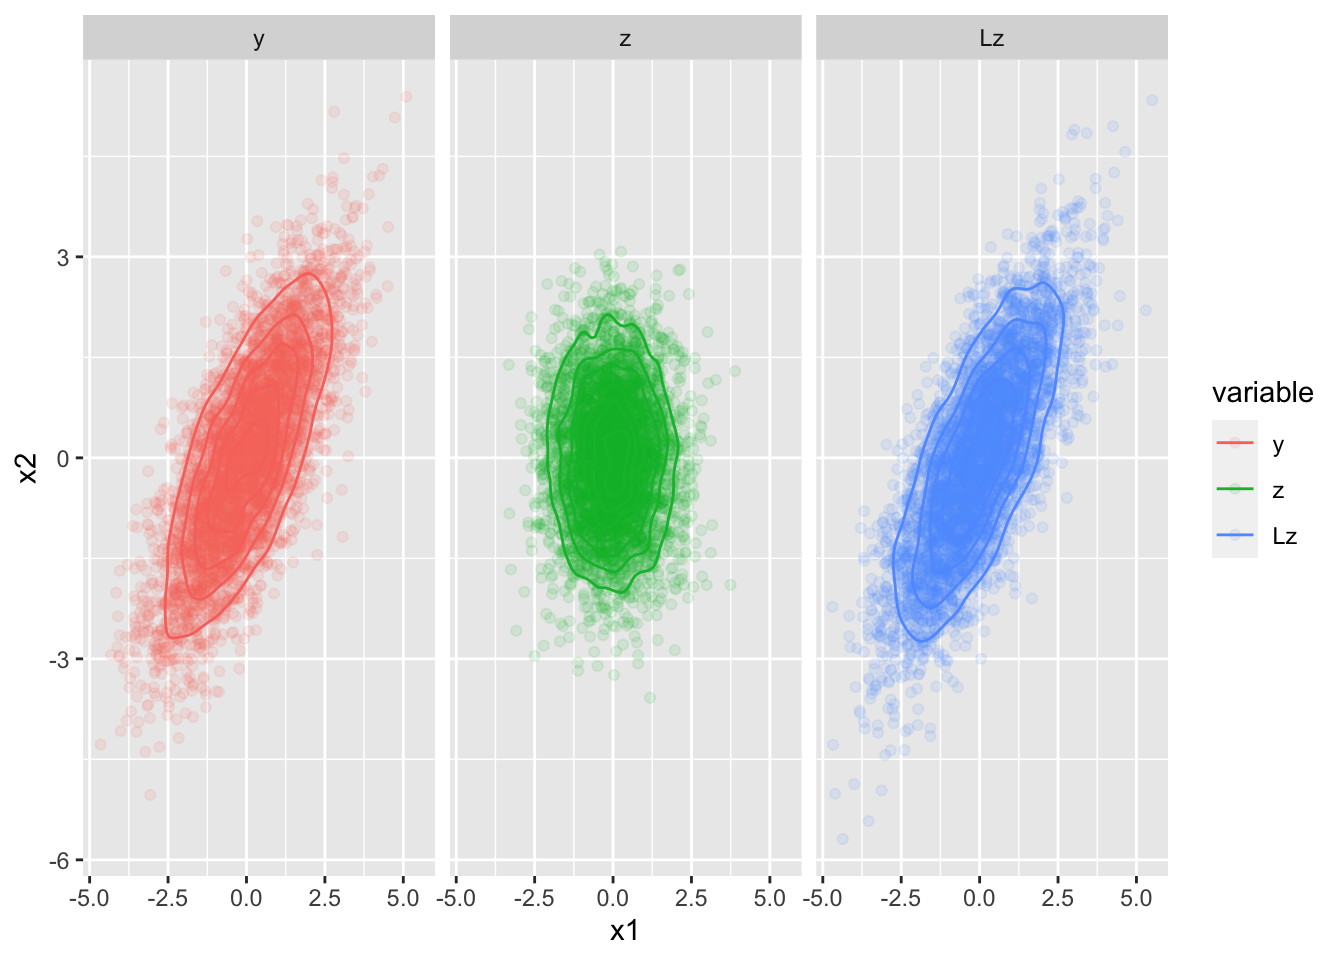
\includegraphics{multivariable-math_files/figure-latex/unnamed-chunk-111-1.pdf}

\hypertarget{subspaces-Rn}{%
\chapter{\texorpdfstring{Subspaces of \(\mathcal{R}^n\)}{Subspaces of \textbackslash mathcal\{R\}\^{}n}}\label{subspaces-Rn}}

\begin{itemize}
\item
  \href{https://www.3blue1brown.com/lessons/span}{3 Blue 1 Brown -- Linear combinations, span, and basis vectors}
\item
  \href{https://www.3blue1brown.com/lessons/inverse-matrices}{3 Blue 1 Brown -- Inverse Matrices, column space, and null space}
\end{itemize}

\begin{Shaded}
\begin{Highlighting}[]
\KeywordTok{library}\NormalTok{(dasc2594)}
\end{Highlighting}
\end{Shaded}

First, let's recall the definition of a subset. A set \(A\) is a subset of a set \(B\) if all elements of \(A\) are also members of \(B\). For example, the integers \(\mathcal{Z}\) are a subset of the real numbers \(\mathbf{R}\) (\(\mathcal{Z} \subset \mathcal{R}\)) and the real numbers are a subset of the complex numbers \(\mathcal{C}\) (\(\mathcal{R} \subset \mathcal{C}\)).

Subspaces are a generalization of the idea of subsets that are useful for understanding vector spaces.

\begin{definition}
\protect\hypertarget{def:subspace}{}\label{def:subspace}

A subspace \(\mathcal{H}\) of \(\mathcal{R}^n\) is a set that has the properties

\begin{enumerate}
\def\labelenumi{\arabic{enumi})}
\item
  The zero vector \(\mathbf{0} \in \mathcal{H}\) \hfill \hfill [(additive identity)]{style="float:right"}
\item
  For each \(\mathbf{u}, \mathbf{v} \in \mathcal{H}\), the sum \(\mathbf{u} + \mathbf{v}\) is in \(\mathcal{H}\) \hfill [(closed under vector addition)]{style="float:right"}
\item
  For each \(\mathbf{u} \in \mathcal{H}\) and scalar \(c\), the scalar multiple \(c \mathbf{u}\) is in \(\mathcal{H}\) \hfill [(closed under scalar multiplication)]{style="float:right"}
\end{enumerate}

\end{definition}

\begin{example}
Let \(\mathbf{u}\) and \(\mathbf{v}\) be vectors in \(\mathcal{R}^n\). Then the vector space defined by span\(\{\mathbf{u}, \mathbf{v} \}\) is a subspace of \(\mathcal{R}^n\)
\end{example}

\begin{solution}
To show that span\(\{\mathbf{u}, \mathbf{v}\}\) is a subspace of \(\mathcal{R}^n\), we must satisfy the three conditions of definition (\ref{def:subspace}).

\begin{enumerate}
\def\labelenumi{\arabic{enumi})}
\item
  \(\mathbf{0} \in \mbox{span}\{\mathbf{u}, \mathbf{v}\}\) because \(\mathbf{0} = 0 \mathbf{u} + 0 \mathbf{v}\) is a linear combination of \(\mathbf{u}\) and \(\mathbf{v}\) with coefficients 0 and 0.
\item
  Let \(\mathbf{x} \in \mbox{span}\{\mathbf{u}, \mathbf{v}\}\) and \(\mathbf{y} \in \mbox{span}\{\mathbf{u}, \mathbf{v}\}\). Then, by the definition of the span (Definition (\ref{def:span})) there exists constants \(a, b, c, d\) such that \(\mathbf{x} = a \mathbf{u} + b \mathbf{v}\) and \(\mathbf{y} = c \mathbf{u} + d \mathbf{v}\). Thus, \(\mathbf{x} + \mathbf{y} = a \mathbf{u} + b \mathbf{v} + c \mathbf{u} + d \mathbf{v} = (a + c) \mathbf{u} + (b + d) \mathbf{v}\) which, by definition, is in the span\(\{\mathbf{u}, \mathbf{v}\}\). Thus, span\(\{\mathbf{u}, \mathbf{v}\}\) is closed under addition.
\item
  Let \(\mathbf{x} \in \mbox{span}\{\mathbf{u}, \mathbf{v}\}\) \(c\) be a constant. Because \(\mathbf{x} \in \mbox{span}\{\mathbf{u}, \mathbf{v}\}\), the definition of the span (Definition (\ref{def:span})) implies there exists constants \(a\) and \(b\) such that \(\mathbf{x} = a \mathbf{u} + b \mathbf{v}\). Thus, \(c\mathbf{x} = ca \mathbf{u} + cb \mathbf{v}\) which is a linear combination of \(\mathbf{u}\) and \(\mathbf{v}\) and is therefore \(c\mathbf{x} \in \mbox{span}\{\mathbf{u}, \mathbf{v}\}\).
\end{enumerate}

Because all three requirements are met, we have shown that \(\mbox{span}\{\mathbf{u}, \mathbf{v}\}\) is a subspace of \(\mathcal{R}^n\).
\end{solution}

\begin{example}

Recall that a solution to the matrix equation \(\mathbf{A} \mathbf{x} = \mathbf{0}\) that has one free variable is a line through the origin and the solution to the matrix equation \(\mathbf{A} \mathbf{x} = \mathbf{b}\) that has one free variable is a line parallel to the prior line that does not go through the origin.

\begin{enumerate}
\def\labelenumi{\Alph{enumi})}
\item
  Is a line through the origin a subspace?
\item
  Is a line \textbf{not} through the origin a subspace?
\end{enumerate}

\end{example}

\begin{solution}

\textbf{Part A:} First, we will consider whether the line through the origin is a subspace. To show this, we need to verify the three properties of a subspace in Definition (\ref{def:subspace})

\begin{enumerate}
\def\labelenumi{\arabic{enumi})}
\item
  \(\mathbf{0}\) is on the line through the origin because \(\mathbf{A} \mathbf{x} = \mathbf{0}\) has the trivial solution \(\mathbf{x} = \mathbf{0}\).
\item
  If \(\mathbf{u}\) and \(\mathbf{v}\) are on the line through the origin, then because the line through the origin is defined as the solution set of the equation \(\mathbf{A} \mathbf{x} = \mathbf{0}\) we know that
  \[
  \begin{aligned}
  \mathbf{A} \mathbf{u} = \mathbf{0} && \mbox{ and } && \mathbf{A} \mathbf{v} = \mathbf{0}.
  \end{aligned}
  \]
  Then, the vector \(\mathbf{u} + \mathbf{v}\) is in the subspace defined by the line through the origin because
  \[
  \begin{aligned}
  \mathbf{A} (\mathbf{u} + \mathbf{v}) = \mathbf{A} \mathbf{u} + \mathbf{A} \mathbf{v} = \mathbf{0} + \mathbf{0} = \mathbf{0},
  \end{aligned}
  \]
  which is a solution to the matrix equation and therefore \(\mathbf{u} + \mathbf{v}\) is a point on the line through the origin.
\item
  If \(\mathbf{u}\) is a point on the line through the origin and \(c\) is a scalar, then because the line through the origin is defined as the solution set of the equation \(\mathbf{A} \mathbf{x} = \mathbf{0}\) we know that
  \[
  \begin{aligned}
  \mathbf{A} \mathbf{u} = \mathbf{0}.
  \end{aligned}
  \]
  Then, the vector \(c \mathbf{u}\) is in the subspace defined by the line through the origin because
  \[
  \begin{aligned}
  \mathbf{A} (c \mathbf{u}) = c \mathbf{A} \mathbf{u}  = c \mathbf{0} = \mathbf{0},
  \end{aligned}
  \]
  which is a solution to the matrix equation and therefore \(c \mathbf{u}\) is a point on the line through the origin.
\end{enumerate}

\textbf{Part B:} Next, we consider whether the line \textbf{not} through the origin is a subspace. To show this, we need to verify the three properties of a subspace in Definition (\ref{def:subspace}). Recall that a line not through the origin is a solution set of the matrix equation \(\mathbf{A} \mathbf{x} = \mathbf{b}\) where the solution set has a single free variable and \(\mathbf \neq \mathbf{0}\). To check if this line defines a subspace, we check the first condition of Definition (\ref{def:subspace})

\begin{enumerate}
\def\labelenumi{\arabic{enumi})}
\tightlist
\item
  \(\mathbf{0}\) is not on the line through the origin because \(\mathbf{A} \mathbf{x} = \mathbf{b}\) does not have the trivial solution \(\mathbf{x} = \mathbf{0}\) because \(\mathbf{A} \mathbf{0} = \mathbf{0} \neq \mathbf{b}\). Because \(\mathbf{0}\) is not a point on the line not through the origin, the line not through the origin does not define a subspace.
\end{enumerate}

\end{solution}

\begin{itemize}
\tightlist
\item
  \textbf{Note:} For any vectors \(\mathbf{u}_1, \ldots, \mathbf{u}_k \in \mathcal{R}^n\), the span\(\{\mathbf{u}_1, \ldots, \mathbf{u}_k\}\) is a subspace of \(\mathcal{R}^n\).
\end{itemize}

\hypertarget{special-subspaces-column-space-and-null-space}{%
\section{Special subspaces: column space and null space}\label{special-subspaces-column-space-and-null-space}}

\begin{definition}
\protect\hypertarget{def:column-space}{}\label{def:column-space}The \textbf{column space}, denoted \(\operatorname{col}(\mathbf{A})\), of a \(m \times n\) matrix \(\mathbf{A}\) which has columns \(\mathbf{a}_1, \ldots, \mathbf{a}_n \in \mathcal{R}^m\) is the set of vectors that are linear combinations of the columns of \(\mathbf{A}\) which is equivalent to the span\(\{\mathbf{a}_1, \ldots, \mathbf{a}_n\}\).
\end{definition}

\begin{example}
Given the matrix \(\mathbf{A} = \begin{pmatrix} 1 & -8 & -9 \\ -3 & 3 & -5 \\ 1 & 0 & 6 \\ -2 & -1 & -1 \end{pmatrix}\) with columns \(\mathbf{a}_1\), \(\mathbf{a}_2\), and \(\mathbf{a}_3\), what is the column space of \(\mathbf{A}\)?
\end{example}

\begin{solution}
Given the matrix \(\mathbf{A} = \begin{pmatrix} 1 & -8 & -9 \\ -3 & 3 & -5 \\ 1 & 0 & 6 \\ -2 & -1 & -1 \end{pmatrix}\) with columns \(\mathbf{a}_1\), \(\mathbf{a}_2\), and \(\mathbf{a}_3\), the column space of \(\mathbf{A}\) is the set of vectors \(\mathbf{b}\) such that
\[
\begin{aligned}
\mathbf{b} = x_1 \mathbf{a_1} + x_2 \mathbf{a}_2 + x_3 \mathbf{a}_3.
\end{aligned}
\]
Thus, the column space of \(\mathbf{A}\) is the span of the vectors that makes up the columns of \(\mathbf{A}\).
\end{solution}

\begin{definition}
\protect\hypertarget{def:null-space}{}\label{def:null-space}The \textbf{null space}, denoted \(\operatorname{null}(\mathbf{A})\), of a matrix \(\mathbf{A}\) is the set of all solutions to the homogeneous matrix equation \(\mathbf{A} \mathbf{x} = \mathbf{0}\).
\end{definition}

While the idea of a null space might at first glance seem unclear, the null space is the set of all vectors which the matrix transformation defined by \(\mathbf{A}\) maps to \(\mathbf{0}\). In other words, the null space of \(\mathbf{A}\) is the set of vectors \(\{ \mathbf{x} : \mathbf{A} \mathbf{x} = \mathbf{0} \}\).

\begin{example}
Given the matrix \(\mathbf{A} = \begin{pmatrix} -3 & -3 & -4 & -5 & -2 \\ -4 & 2 & -4 & 5 & 3 \\ 4 & -4 & 4 & -3 & 5 \end{pmatrix}\) with columns \(\mathbf{a}_1\), \(\mathbf{a}_2\), \(\mathbf{a}_3\), and \(\mathbf{a}_4\), find vectors that span the null space of \(\mathbf{A}\).
\end{example}

\begin{solution}

Given the matrix \(\mathbf{A} = \begin{pmatrix} -3 & -3 & -4 & -5 & -2 \\ -4 & 2 & -4 & 5 & 3 \\ 4 & -4 & 4 & -3 & 5 \end{pmatrix}\) with columns \(\mathbf{a}_1\), \(\mathbf{a}_2\), \(\mathbf{a}_3\), and \(\mathbf{a}_4\), the null space of \(\mathbf{A}\) is the solution set of the homogeneous system of equations \(\mathbf{A} \mathbf{x} = \mathbf{0}\). Using an augmented matrix and transforming into reduced row echelon form gives the RREF form
\[
\begin{aligned}
\begin{pmatrix} -3 & -3 & -4 & -5 & -2 & 0 \\ -4 & 2 & -4 & 5 & 3 & 0 \\ 4 & -4 & 4 & -3 & 5 & 0 \end{pmatrix} \sim \begin{pmatrix} 1 & 0 & 0 & -15 & -25 & 0 \\ 0 & 1 & 0 & -1 & -4 & 0 \\ 0 & 0 & 1 & 53/4 & 89/4 & 0 \end{pmatrix}
\end{aligned}
\]
which tells us that the solution to the system of equations is
\[
\begin{aligned}
x_1 - 15 x_4 -25 x_5 & = 0 \\
x_2 - x_4 - 4 x_5 & = 0 \\
x_3 + \frac{53}{4} x_4  + \frac{89}{4} x_5 & = 0\\
x_4 & = x_4 \\
x_5 & = x_5
\end{aligned}
\]
Writing this solution as a vector times \(x_4\) and a vector times \(x_5\) gives the vectors \(\begin{pmatrix} 15 \\ 1 \\ -\frac{53}{4} \\ 1 \\ 0 \end{pmatrix}\) and \(\begin{pmatrix} 25 \\ 4 \\ -\frac{89}{4} \\ 0 \\ 1 \end{pmatrix}\).

In \texttt{R}, this is shown by starting with the matrix \texttt{A}

\begin{Shaded}
\begin{Highlighting}[]
\NormalTok{A <-}\StringTok{ }\KeywordTok{matrix}\NormalTok{(}\KeywordTok{c}\NormalTok{(}\OperatorTok{-}\DecValTok{3}\NormalTok{, }\DecValTok{-4}\NormalTok{, }\DecValTok{4}\NormalTok{, }\DecValTok{-3}\NormalTok{, }\DecValTok{2}\NormalTok{, }\DecValTok{-4}\NormalTok{, }\DecValTok{-4}\NormalTok{, }\DecValTok{-4}\NormalTok{, }\DecValTok{4}\NormalTok{, }\DecValTok{-5}\NormalTok{, }\DecValTok{5}\NormalTok{, }\DecValTok{-3}\NormalTok{, }\DecValTok{-2}\NormalTok{, }\DecValTok{3}\NormalTok{, }\DecValTok{5}\NormalTok{), }\DecValTok{3}\NormalTok{, }\DecValTok{5}\NormalTok{)}
\NormalTok{A}
\end{Highlighting}
\end{Shaded}

\begin{verbatim}
##      [,1] [,2] [,3] [,4] [,5]
## [1,]   -3   -3   -4   -5   -2
## [2,]   -4    2   -4    5    3
## [3,]    4   -4    4   -3    5
\end{verbatim}

Looking at the reduced row echelon form of \(\mathbf{A}\) gives

\begin{Shaded}
\begin{Highlighting}[]
\KeywordTok{rref}\NormalTok{(A)}
\end{Highlighting}
\end{Shaded}

\begin{verbatim}
##      [,1] [,2] [,3]   [,4]   [,5]
## [1,]    1    0    0 -15.00 -25.00
## [2,]    0    1    0  -1.00  -4.00
## [3,]    0    0    1  13.25  22.25
\end{verbatim}

where the columns of interest are the non-pivot columns. For this matrix \(\mathbf{A}\), the fourth and fifth columns of \(\mathbf{A}\) are the non-pivot columns. The fourth column or the RREF form corresponds to the variable \(x_4\) and the fifth column corresponds to the variable \(x_5\). Thus, you can extract the vectors that form the null space from these fourth and fifth columns of the RREF form of \(\mathbf{A}\) like so

\begin{Shaded}
\begin{Highlighting}[]
\CommentTok{# the nullspace vector corresponding to x4 = 1 and x5 = 0}
\KeywordTok{c}\NormalTok{(}\OperatorTok{-}\KeywordTok{rref}\NormalTok{(A)[, }\DecValTok{4}\NormalTok{], }\DecValTok{1}\NormalTok{, }\DecValTok{0}\NormalTok{)}
\end{Highlighting}
\end{Shaded}

\begin{verbatim}
## [1]  15.00   1.00 -13.25   1.00   0.00
\end{verbatim}

\begin{Shaded}
\begin{Highlighting}[]
\CommentTok{# the nullspace vector corresponding to x4 = 0 and x5 = 1}
\KeywordTok{c}\NormalTok{(}\OperatorTok{-}\KeywordTok{rref}\NormalTok{(A)[, }\DecValTok{5}\NormalTok{], }\DecValTok{0}\NormalTok{, }\DecValTok{1}\NormalTok{)}
\end{Highlighting}
\end{Shaded}

\begin{verbatim}
## [1]  25.00   4.00 -22.25   0.00   1.00
\end{verbatim}

We check that these vectors are in null(\(\mathbf{A}\)) by using matrix multiplication and verifying that these are zero (at least up to numeric overflow/underflow)

\begin{Shaded}
\begin{Highlighting}[]
\NormalTok{A }\OperatorTok\StringTok{ }\KeywordTok{c}\NormalTok{(}\OperatorTok{-}\KeywordTok{rref}\NormalTok{(A)[, }\DecValTok{4}\NormalTok{], }\DecValTok{1}\NormalTok{, }\DecValTok{0}\NormalTok{)}
\end{Highlighting}
\end{Shaded}

\begin{verbatim}
##               [,1]
## [1,] -7.105427e-15
## [2,] -7.105427e-15
## [3,]  7.105427e-15
\end{verbatim}

\begin{Shaded}
\begin{Highlighting}[]
\NormalTok{A }\OperatorTok\StringTok{ }\KeywordTok{c}\NormalTok{(}\OperatorTok{-}\KeywordTok{rref}\NormalTok{(A)[, }\DecValTok{5}\NormalTok{], }\DecValTok{0}\NormalTok{, }\DecValTok{1}\NormalTok{)}
\end{Highlighting}
\end{Shaded}

\begin{verbatim}
##               [,1]
## [1,] -1.421085e-14
## [2,] -1.421085e-14
## [3,]  1.421085e-14
\end{verbatim}

\end{solution}

\begin{theorem}
The null space of a n \(m \times m\) matrix \(\mathbf{A}\) is a subspace of \(\mathcal{R}^n\).
\end{theorem}

\begin{proof}

Do in class
Show that the three requirements of the defintion of a subspace in Definition (\ref{def:subspace}) are met.

\begin{enumerate}
\def\labelenumi{\arabic{enumi})}
\item
\item
\item
\end{enumerate}

\end{proof}

\begin{itemize}
\tightlist
\item
  Example: give \(\mathbf{A}\) and \(\mathbf{x}\) and determine if \(\mathbf{x}\) is in the null space of \(\mathbf{A}\) using \texttt{R}
\end{itemize}

\hypertarget{the-basis-of-a-subspace}{%
\section{The basis of a subspace}\label{the-basis-of-a-subspace}}

\begin{definition}
\protect\hypertarget{def:basis}{}\label{def:basis}A \textbf{basis} for a subspace \(\mathcal{H}\) of \(\mathcal{R}^n\) is

\begin{enumerate}
\def\labelenumi{\arabic{enumi})}
\tightlist
\item
  a linearly independent set in \(\mathcal{H}\) that
\item
  spans \(\mathbf{H}\).
\end{enumerate}

Equivlently, a baisis is a set of linearly independent vectors \(\mathbf{u}_1, \ldots, \mathbf{u}_k\) such that span\(\{\mathbf{u}_1, \ldots, \mathbf{u}_k\} = \mathcal{H}\).
\end{definition}

The requirement that the vectors of a basis are linearly independent while spanning a subspace \(\mathcal{H}\) means that a basis is a \textbf{minimal spanning set} for the subspace \(\mathcal{H}\)

\begin{example}
Is a basis for a vector space unique?
\end{example}

\begin{solution}
A basis for a vector is not unique. Just like you can represent the number 16 as \(1.6 * 10^1\) (base 10) or \(2^4\) (base 2), the basis for a vector space is also not unique.
\end{solution}

\begin{definition}
\protect\hypertarget{def:standard-basis}{}\label{def:standard-basis}The \textbf{standard basis} for \(\mathcal{R}^n\) is the set of vectors \(\left\{ \mathbf{e}_1, \mathbf{e}_2, \ldots, \mathbf{e}_n \right\}\) of length \(n\) where the vector \(\mathbf{e}_j\) is a vector that is 0 in every value except for a 1 in the \(j\)th position. For example,
\[
\begin{aligned}
\mathbf{e}_1 = \begin{pmatrix} 1 \\ 0 \\ 0 \\ \vdots \\ 0 \end{pmatrix}, && \mathbf{e}_2 = \begin{pmatrix} 0 \\ 1 \\ 0 \\ \vdots \\ 0 \end{pmatrix}, && \mathbf{e}_3 = \begin{pmatrix} 0 \\ 0 \\ 1 \\ \vdots \\ 0\end{pmatrix}, && \ldots, && \mathbf{e}_n = \begin{pmatrix} 0 \\ 0 \\ 0 \\ \vdots \\ 1 \end{pmatrix}.
\end{aligned}
\]
Notice that the matrix defined as having columns \(\mathbf{e}_1, \mathbf{e}_2, \ldots, \mathbf{e}_n\) is the identity matrix \(\mathbf{I}\).
\end{definition}

\begin{example}
What is the standard basis for \(\mathcal{R}^3\)?
\end{example}

\begin{solution}
The standard basis for \(\mathcal{R}^3\) are the x-, y-, and z-axes. These are written as vectors where the x-axis is \(\mathbf{e}_1 = \begin{pmatrix} 1 \\ 0 \\ 0 \end{pmatrix}\), the y-axis is \(\mathbf{e}_2 = \begin{pmatrix} 0 \\ 1 \\ 0 \end{pmatrix}\), and the z-axis is \(\mathbf{e}_3 = \begin{pmatrix} 0 \\ 0 \\ 1\end{pmatrix}\),
\end{solution}

\begin{example}
Do the following set of vectors form a basis for \(\mathcal{R}^3\)?

\(\mathbf{x} = \begin{pmatrix} 2 \\ 1 \\ 2 \end{pmatrix}\), \(\mathbf{y} = \begin{pmatrix} -1 \\ 1 \\ 1 \end{pmatrix}\), and \(\mathbf{z} = \begin{pmatrix} 1 \\ 0 \\ 2 \end{pmatrix}\)
\end{example}

\begin{solution}
For the set of vectors \(\mathbf{x} = \begin{pmatrix} 2 \\ 1 \\ 2 \end{pmatrix}\), \(\mathbf{y} = \begin{pmatrix} -1 \\ 1 \\ 1 \end{pmatrix}\), and \(\mathbf{z} = \begin{pmatrix} 1 \\ 0 \\ 2 \end{pmatrix}\) to form a basis for \(\mathcal{R}^3\), we need to satisfy the two conditions in Definition (\ref{def:basis}). Both conditions of Definition (\ref{def:basis}) can be checked by combining the set of vectors \(\mathbf{x}\), \(\mathbf{y}\), and \(\mathbf{z}\) into a matrix and using RREF to determine the span\(\{ \mathbf{x}, \mathbf{y}, \mathbf{z} \}\) and determine whether the set of vectors \(\{ \mathbf{x}, \mathbf{y}, \mathbf{z} \}\) is linearly independent. The matrix of the vectors is
\[
\begin{pmatrix} 2 & -1 & 1 \\ 1 & 1 & 0 \\ 2 & 1 & 2 \end{pmatrix}
\]
which is row-equivalent to
\[
\begin{pmatrix} 1 & 0 & 0 \\ 0 & 1 & 0 \\ 0 & 0 & 1 \end{pmatrix}
\]
Because the reduced row echelon form of the matrix has 3 pivot columns, the span\(\{ \mathbf{x}, \mathbf{y}, \mathbf{z} \} = \mathcal{R}^3\) which satisfies the first condition for being a basis. Because there is a pivot in every column, we know the set of vectors is linearly independent which satisfies the second condition for being a basis. Therefore, the set of vectors \(\{ \mathbf{x}, \mathbf{y}, \mathbf{z} \}\) forms a basis for \(\mathcal{R}^3\)

Using \texttt{R}, we can show this result first by creating the vectors \texttt{x}, \texttt{y}, and \texttt{z} and then joining these into a matrix \texttt{A} using \texttt{cbind()}

\begin{Shaded}
\begin{Highlighting}[]
\NormalTok{x <-}\StringTok{ }\KeywordTok{c}\NormalTok{(}\DecValTok{2}\NormalTok{, }\DecValTok{1}\NormalTok{, }\DecValTok{2}\NormalTok{)}
\NormalTok{y <-}\StringTok{ }\KeywordTok{c}\NormalTok{(}\OperatorTok{-}\DecValTok{1}\NormalTok{, }\DecValTok{1}\NormalTok{, }\DecValTok{1}\NormalTok{)}
\NormalTok{z <-}\StringTok{ }\KeywordTok{c}\NormalTok{(}\DecValTok{1}\NormalTok{, }\DecValTok{0}\NormalTok{, }\DecValTok{2}\NormalTok{)}

\NormalTok{A <-}\StringTok{ }\KeywordTok{cbind}\NormalTok{(x, y, z)}
\end{Highlighting}
\end{Shaded}

Next, we convert \texttt{A} to reduced row echelon form to get the row equivalent matrix

\begin{Shaded}
\begin{Highlighting}[]
\KeywordTok{rref}\NormalTok{(A)}
\end{Highlighting}
\end{Shaded}

\begin{verbatim}
##      x y z
## [1,] 1 0 0
## [2,] 0 1 0
## [3,] 0 0 1
\end{verbatim}

Because this reduced row echelon form has a pivot in each column we know the columns of the matrix \texttt{A} are linearly independent. Because there are 3 pivot columns in total, we know the span of the columns of \texttt{A} is \(\mathcal{R}^3\). Therefore, the vectors \(\mathbf{x}, \mathbf{y}, \mathbf{z}\) forms a basis for \(\mathcal{R}^3\).
\end{solution}

\begin{example}
Do the following set of vectors form a basis for \(\mathcal{R}^3\)?

\(\mathbf{w} = \begin{pmatrix} 2 \\ 1 \\ 2 \end{pmatrix}\), \(\mathbf{x} = \begin{pmatrix} -1 \\ 1 \\ 1 \end{pmatrix}\), \(\mathbf{y} = \begin{pmatrix} 1 \\ 0 \\ 2 \end{pmatrix}\), and \(\mathbf{z} = \begin{pmatrix} 4 \\ 2 \\ -2 \end{pmatrix}\)
\end{example}

\begin{solution}
For the set of vectors \(\mathbf{w} = \begin{pmatrix} 2 \\ 1 \\ 2 \end{pmatrix}\), \(\mathbf{x} = \begin{pmatrix} -1 \\ 1 \\ 1 \end{pmatrix}\), \(\mathbf{y} = \begin{pmatrix} 1 \\ 0 \\ 2 \end{pmatrix}\), and \(\mathbf{z} = \begin{pmatrix} 4 \\ 2 \\ -2 \end{pmatrix}\) to form a basis for \(\mathcal{R}^3\), we need to satisfy the two conditions in Definition (\ref{def:basis}). Both conditions of Definition (\ref{def:basis}) can be checked by combining the set of vectors \(\mathbf{w}\), \(\mathbf{x}\), \(\mathbf{y}\), and \(\mathbf{z}\) into a matrix and using RREF to determine the span\(\{ \mathbf{w}, \mathbf{x}, \mathbf{y}, \mathbf{z} \}\) and determine whether the set of vectors \(\{ \mathbf{w}, \mathbf{x}, \mathbf{y}, \mathbf{z} \}\) is linearly independent. The matrix of the vectors is
\[
\begin{pmatrix} 2 & -1 & 1 & 4 \\ 1 & 1 & 0 & 2 \\ 2 & 1 & 2 & -2 \end{pmatrix}
\]
which is row-equivalent to
\[
\begin{pmatrix} 1 & 0 & 0 & 16/5 \\ 0 & 1 & 0 & -6/5 \\ 0 & 0 & 1 & -18/5 \end{pmatrix}
\]
Because the reduced row echelon form of the matrix has 3 pivot columns, the span\(\{ \mathbf{x}, \mathbf{y}, \mathbf{z} \} = \mathcal{R}^3\) which satisfies the first condition for being a basis. However, there is not a pivot in every column which tells us that the set of vectors is linearly dependent which does not satisfy the second condition for being a basis. Therefore, the set of vectors \(\{ \mathbf{w}, \mathbf{x}, \mathbf{y}, \mathbf{z} \}\) do not form a basis for \(\mathcal{R}^3\)

Using \texttt{R}, we can show this result first by creating the vectors \texttt{w}, x\texttt{,}y\texttt{,\ and}z\texttt{and\ then\ joining\ these\ into\ a\ matrix}A\texttt{using}cbind()`

\begin{Shaded}
\begin{Highlighting}[]
\NormalTok{w <-}\StringTok{ }\KeywordTok{c}\NormalTok{(}\DecValTok{2}\NormalTok{, }\DecValTok{1}\NormalTok{, }\DecValTok{2}\NormalTok{)}
\NormalTok{x <-}\StringTok{ }\KeywordTok{c}\NormalTok{(}\OperatorTok{-}\DecValTok{1}\NormalTok{, }\DecValTok{1}\NormalTok{, }\DecValTok{1}\NormalTok{)}
\NormalTok{y <-}\StringTok{ }\KeywordTok{c}\NormalTok{(}\DecValTok{1}\NormalTok{, }\DecValTok{0}\NormalTok{, }\DecValTok{2}\NormalTok{)}
\NormalTok{z <-}\StringTok{ }\KeywordTok{c}\NormalTok{(}\DecValTok{4}\NormalTok{, }\DecValTok{2}\NormalTok{, }\DecValTok{-2}\NormalTok{)}

\NormalTok{A <-}\StringTok{ }\KeywordTok{cbind}\NormalTok{(w, x, y, z)}
\end{Highlighting}
\end{Shaded}

Next, we convert \texttt{A} to reduced row echelon form to get the row equivalent matrix

\begin{Shaded}
\begin{Highlighting}[]
\KeywordTok{rref}\NormalTok{(A)}
\end{Highlighting}
\end{Shaded}

\begin{verbatim}
##      w x y    z
## [1,] 1 0 0  3.2
## [2,] 0 1 0 -1.2
## [3,] 0 0 1 -3.6
\end{verbatim}

Because this reduced row echelon form does not have a pivot in each column, we know the columns of the matrix \texttt{A} are linearly dependent. Because there are 3 pivot columns in total, we know the span of the columns of \texttt{A} is \(\mathcal{R}^3\). Because the set of vectors \(\{ \mathbf{w}, \mathbf{x}, \mathbf{y}, \mathbf{z} \}\) are linearly dependent, they do not form a basis for \(\mathcal{R}^3\).
\end{solution}

\begin{example}
Do the following set of vectors form a basis for \(\mathcal{R}^3\)?

\(\mathbf{x} = \begin{pmatrix} 4 \\ 3 \\ 2 \end{pmatrix}\), \(\mathbf{y} = \begin{pmatrix} 3 \\ -3 \\ 4 \end{pmatrix}\), and \(\mathbf{z} = \begin{pmatrix} 5 \\ 9 \\ 0 \end{pmatrix}\)
\end{example}

\begin{solution}
For the set of vectors \(\mathbf{x} = \begin{pmatrix} 4 \\ 3 \\ 2 \end{pmatrix}\), \(\mathbf{y} = \begin{pmatrix} 3 \\ -3 \\ 4 \end{pmatrix}\), and \(\mathbf{z} = \begin{pmatrix} 5 \\ 9 \\ 0 \end{pmatrix}\) to form a basis for \(\mathcal{R}^3\), we need to satisfy the two conditions in Definition (\ref{def:basis}). Both conditions of Definition (\ref{def:basis}) can be checked by combining the set of vectors \(\mathbf{x}\), \(\mathbf{y}\), and \(\mathbf{z}\) into a matrix and using RREF to determine the span\(\{ \mathbf{x}, \mathbf{y}, \mathbf{z} \}\) and determine whether the set of vectors \(\{ \mathbf{x}, \mathbf{y}, \mathbf{z} \}\) is linearly independent. The matrix of the vectors is
\[
\begin{pmatrix} 4 & 3 & 5 \\ 3 & -3 & 9 \\ 2 & 4 & 0 \end{pmatrix}
\]
which is row-equivalent to
\[
\begin{pmatrix} 1 & 0 & 2 \\ 0 & 1 & -1 \\ 0 & 0 & 0 \end{pmatrix}
\]
Because the reduced row echelon form of the matrix has 2 pivot columns, the span\(\{ \mathbf{x}, \mathbf{y}, \mathbf{z} \} = \mathcal{R}^2\) which does not satisfy the first condition for being a basis for \(\mathcal{R}^3\). In addition, there is not a pivot in every column which tells us that the set of vectors is linearly dependent which does not satisfy the second condition for being a basis. Therefore, the set of vectors \(\{ \mathbf{x}, \mathbf{y}, \mathbf{z} \}\) do not form a basis for \(\mathcal{R}^3\)

Using \texttt{R}, we can show this result first by creating the vectors x\texttt{,}y\texttt{,\ and}z\texttt{and\ then\ joining\ these\ into\ a\ matrix}A\texttt{using}cbind()`

\begin{Shaded}
\begin{Highlighting}[]
\NormalTok{x <-}\StringTok{ }\KeywordTok{c}\NormalTok{(}\DecValTok{4}\NormalTok{, }\DecValTok{3}\NormalTok{, }\DecValTok{2}\NormalTok{)}
\NormalTok{y <-}\StringTok{ }\KeywordTok{c}\NormalTok{(}\DecValTok{3}\NormalTok{, }\DecValTok{-3}\NormalTok{, }\DecValTok{4}\NormalTok{)}
\NormalTok{z <-}\StringTok{ }\KeywordTok{c}\NormalTok{(}\DecValTok{5}\NormalTok{, }\DecValTok{9}\NormalTok{, }\DecValTok{0}\NormalTok{)}

\NormalTok{A <-}\StringTok{ }\KeywordTok{cbind}\NormalTok{(x, y, z)}
\end{Highlighting}
\end{Shaded}

Next, we convert \texttt{A} to reduced row echelon form to get the row equivalent matrix

\begin{Shaded}
\begin{Highlighting}[]
\KeywordTok{rref}\NormalTok{(A)}
\end{Highlighting}
\end{Shaded}

\begin{verbatim}
##      x y  z
## [1,] 1 0  2
## [2,] 0 1 -1
## [3,] 0 0  0
\end{verbatim}

Because this reduced row echelon form does not have a pivot in each column, we know the columns of the matrix \texttt{A} are linearly dependent. Because there are 2 pivot columns in total, we know the span of the columns of \texttt{A} is \(\mathcal{R}^2\) which is not \(\mathcal{R}^3\). Because the set of vectors \(\{ \mathbf{x}, \mathbf{y}, \mathbf{z} \}\) are linearly dependent and do not span \(\mathcal{R}^3\), they do not form a basis for \(\mathcal{R}^3\).
\end{solution}

\begin{example}
Using \texttt{R}, find a basis for the null space of the matrix
\[
\mathbf{A} = \begin{pmatrix} 2 & 4 & 1 & 3 \\ -1 & -2 & 6 & 5 \\ 1 & 2 & -3 & 2 \end{pmatrix}
\]
\end{example}

\begin{solution}

Given the matrix \(\mathbf{A}\), we look for non-trivial solutions to \(\mathbf{A} \mathbf{x} = \mathbf{0}\)

\begin{Shaded}
\begin{Highlighting}[]
\NormalTok{A <-}\StringTok{ }\KeywordTok{matrix}\NormalTok{(}\KeywordTok{c}\NormalTok{(}\DecValTok{2}\NormalTok{, }\DecValTok{-1}\NormalTok{, }\DecValTok{1}\NormalTok{, }\DecValTok{4}\NormalTok{, }\DecValTok{-2}\NormalTok{, }\DecValTok{2}\NormalTok{, }\DecValTok{1}\NormalTok{, }\DecValTok{6}\NormalTok{, }\DecValTok{-3}\NormalTok{, }\DecValTok{3}\NormalTok{, }\DecValTok{5}\NormalTok{, }\DecValTok{2}\NormalTok{), }\DecValTok{3}\NormalTok{, }\DecValTok{4}\NormalTok{)}
\KeywordTok{rref}\NormalTok{(}\KeywordTok{cbind}\NormalTok{(A, }\DecValTok{0}\NormalTok{))}
\end{Highlighting}
\end{Shaded}

\begin{verbatim}
##      [,1] [,2] [,3] [,4] [,5]
## [1,]    1    2    0    0    0
## [2,]    0    0    1    0    0
## [3,]    0    0    0    1    0
\end{verbatim}

which has solution \(x_1 = -2 x_2\), \(x_2 = \mbox{free}\), \(x_3 = 0\) and \(x_4 = 0\). This can be represented as a vector \(\mathbf{v} = \begin{pmatrix} -2 \\ 1 \\ 0 \\ 0 \end{pmatrix}\). Thus, \(\left\{ \begin{pmatrix} -2 \\ 1 \\ 0 \\ 0 \end{pmatrix} \right\}\) is a basis for the null space of \(\mathbf{A}\).

We can check this by showing that \(\mathbf{A} \mathbf{v} = \mathbf{0}\)

\begin{Shaded}
\begin{Highlighting}[]
\NormalTok{v <-}\StringTok{ }\KeywordTok{c}\NormalTok{(}\OperatorTok{-}\DecValTok{2}\NormalTok{, }\DecValTok{1}\NormalTok{, }\DecValTok{0}\NormalTok{, }\DecValTok{0}\NormalTok{)}
\NormalTok{A }\OperatorTok\StringTok{ }\NormalTok{v}
\end{Highlighting}
\end{Shaded}

\begin{verbatim}
##      [,1]
## [1,]    0
## [2,]    0
## [3,]    0
\end{verbatim}

In addition, any linear combination of the basis is also in the null space

\begin{Shaded}
\begin{Highlighting}[]
\NormalTok{A }\OperatorTok\StringTok{ }\NormalTok{(}\DecValTok{5}\OperatorTok{*}\NormalTok{v)}
\end{Highlighting}
\end{Shaded}

\begin{verbatim}
##      [,1]
## [1,]    0
## [2,]    0
## [3,]    0
\end{verbatim}

\end{solution}

\begin{theorem}
The pivot columns of a matrix \(\mathbf{A}\) form a basis for the column space of \(\mathbf{A}\).
\end{theorem}

\textbf{Note:} Use the columns of \(\mathbf{A}\), not the columns of the matrix in echelon form.

\begin{proof}
We will provide just a sketch of the proof here. First, the column space (Definition \ref{def:column-space}) is the space defined by the linear combination of the columns of \(\mathbf{A}\). Thus, the span of any subset of the vectors that make up the columns of \(\mathbf{A}\) must, by definition, be in the column space of \(\mathbf{A}\), because any linear combination of the subset of vectors is just a linear combination of the full set of vectors with the coefficients of the vectors in the subset with the same coefficients and the coefficients of the vectors not in the subset equal to 0. Thus, the span of the subset of the vectors is contained within the span of the columns of \(\mathbf{A}\), which is defined as the column space.

Now, choose the subset of columns of \(\mathbf{A}\) that correspond to the pivot columns of the reduced row echelon form of \(\mathbf{A}\). If the span of the columns of \(\mathbf{A} = \mathcal{R}^p\), then 1) there must be \(p\) pivot columns in the reduced row echelon form of \(\mathbf{A}\) and 2) there are \(p\) vectors in the subset of vectors where the columns of \(\mathbf{A}\) are pivot columns. Thus, the subset of vectors spans \(\mathcal{R}^p\) (the columnspace) and, by definition, there are \(p\) pivot columns (therefore there is a pivot in each column) so the subset of vectors defined by the pivot columns of \(\mathbf{A}\) are linearly independent.
\end{proof}

\begin{example}
Find a basis for the column space of the matrix
\[
\mathbf{A} = \begin{pmatrix} 3 & 1 & 2 & -3 \\ 4 & 1 & -3 & -2 \\ 4 & -1 & -3 & 1 \end{pmatrix}
\]
\end{example}

\begin{solution}
Given the matrix \(\mathbf{A}\), we first find its reduced row echelon form
\[
\begin{pmatrix} 1 & 0 & 0 & -11/34 \\ 0 & 1 & 0 & -3/2 \\ 0 & 0 & 1 & -9/34 \end{pmatrix}
\]
which has pivots in the first three columns. Thus, the column space of \(\mathbf{A}\), which is defined as the linear combination of the vectors of \(\mathbf{A}\), spans \(\mathcal{R}^3\) because there are three pivot columns. The first three columns of \(\mathbf{A}\) are \(\begin{pmatrix} 3 \\ 4 \\ 4 \end{pmatrix}\), \(\begin{pmatrix} 1 \\ 1 \\ -1 \end{pmatrix}\), and \(\begin{pmatrix} 2 \\ -3 \\ -3 \end{pmatrix}\). Because these 3 vectors are linearly independent (they are each pivot columns in the reduced row echelon form of \(\mathbf{A}\)) and they span \(\mathcal{R}^3\), they form a basis for the column space of \(\mathbf{A}\).

Thus, any vector in the columns space of \(\mathbf{A}\) (for example, the fourth column of \(\mathbf{A}\)) can be written as a linear combination of the basis vectors of the columns space of \(\mathbf{A}\).
\end{solution}

\begin{example}
Find a basis for the column space of the matrix
\[
\begin{pmatrix} -4 & 1 \\ 8 & -2 \\ 6 & 3 \\ 9 & 7 \end{pmatrix}
\]
\end{example}

\begin{solution}
Given the matrix \(\mathbf{A}\), we first find its reduced row echelon form
\[
\begin{pmatrix} 1 & 0 \\ 0 & 1 \\ 0 & 0 \\ 0 & 0 \end{pmatrix}
\]
which has pivots in the first two columns. Thus, the column space of \(\mathbf{A}\), which is defined as the linear combination of the vectors of \(\mathbf{A}\), spans \(\mathcal{R}^2\) because there are two pivot columns. The first two columns of \(\mathbf{A}\) are \(\begin{pmatrix} -4 \\ 8 \\ 6 \\ 9 \end{pmatrix}\) and \(\begin{pmatrix} 1 \\ -2 \\ 3 \\ 7 \end{pmatrix}\). Because these 2 vectors are linearly independent (they are each pivot columns) and they span \(\mathcal{R}^2\), they form a basis for the column space of \(\mathbf{A}\).

Note however, that the first two columns of the reduced row echelon form of \(\mathbf{A}\) (the vectors \(\begin{pmatrix} 1 \\ 0 \\ 0 \\ 0 \end{pmatrix}\) and \(\begin{pmatrix} 0 \\ 1 \\ 0 \\ 0 \end{pmatrix}\)) do not form a basis for the column space of \(\mathbf{A}\). This can be seen because The first two columns of \(\mathbf{A}\) have non-zero entries in the 3rd and 4th elements.
\end{solution}

\hypertarget{dimension-and-rank}{%
\chapter{Dimension and Rank}\label{dimension-and-rank}}

\begin{Shaded}
\begin{Highlighting}[]
\KeywordTok{library}\NormalTok{(dasc2594)}
\end{Highlighting}
\end{Shaded}

\hypertarget{coordinate-systems}{%
\section{Coordinate systems}\label{coordinate-systems}}

Recall the idea of polynomials (e.g., a polynomial of order \(p\) is \(a_1x^p + a_2x^{p-1} + \ldots + a_p x^1 + a_{p+1} x^0\)) where the polynomials \(x^p, x^{p-1}, \ldots, x^1, x^0\) form a set of powers up to the power \(p\) of \(x\) from which the coefficients \(a_p, \ldots, a_{p+1}\) can be used to make any polynomial of order \(p\). It can be said that the powers of \(x\) (\(x^p, x^{p-1}, \ldots, x^1, x^0\)) form a basis for all polynomials of order \(p\).

In the previous section, we extended this analogy to vector spaces using the concept of a minimal spanning set. Consider the basis \(\mathbf{b}_1, \ldots, \mathbf{b}_k\) for a subspace \(\mathcal{H}\) of \(\mathcal{R}^n\) where span\(\{\mathbf{b}_1, \ldots, \mathbf{b}_k\} = \mathcal{H}\). Because the set \(\mathbf{b}_1, \ldots, \mathbf{b}_k\) is a basis, the set of vectors is linearly independent. Then, because the set \(\mathbf{b}_1, \ldots, \mathbf{b}_k\) is a basis, we have the following result.

\begin{theorem}
For each vector \(\mathbf{a}\) in the subspace \(\mathcal{H}\) of \(\mathcal{R}^n\), and a basis \(\mathbf{b}_1, \ldots, \mathbf{b}_k\), there is a unique set of coefficients \(x_1, \ldots, x_k\) such that
\[
\begin{aligned}
\mathbf{a} & = x_1 \mathbf{b}_1 + \cdots + x_k \mathbf{b}_k
\end{aligned}
\]
\end{theorem}

\begin{proof}
In class: assume contradiction that there are two ways \(x_1, \ldots, x_k\) and \(y_1, \ldots, y_k\)\ldots{} Show that this violates the assumption of linear dependence.
\end{proof}

\begin{definition}
\protect\hypertarget{def:coordinates}{}\label{def:coordinates}Let \(\mathcal{B} = \{ \mathbf{b}_1, \ldots, \mathbf{b}_k\}\) be a basis for a subspace \(\mathcal{H}\) of \(\mathcal{R}^n\). Then, for each \(\mathbf{a} \in \mathcal{H}\), the \textbf{coordinates} of \(\mathbf{a}\) with respect to the basis \(\mathcal{B}\) are the set of coefficients \(\{x_1, \ldots, x_k\}\) where
\[
\begin{aligned}
\mathbf{a} & = x_1 \mathbf{b}_1 + \cdots + x_k \mathbf{b}_k.
\end{aligned}
\]
\end{definition}

\begin{example}
Let \(\mathcal{B} = \left\{ \mathbf{b}_1 = \begin{pmatrix} 3 \\ 0 \\ 1 \end{pmatrix}, \mathbf{b}_2 = \begin{pmatrix} 2 \\ -3 \\ 1 \end{pmatrix}, \mathbf{b}_3 = \begin{pmatrix} 0 \\ 0 \\ 1 \end{pmatrix} \right\}\) and \(\mathbf{a} = \begin{pmatrix} 5 \\ 6 \\ 1 \end{pmatrix}\). What are the coordinates of \(\mathbf{a}\) with respect to the basis \(\mathcal{B}\)?
\end{example}

\begin{solution}

It can be seen that \(\mathbf{a} = 3 \mathbf{b}_1 - 2 \mathbf{b}_2 + 0 \mathbf{b}_3\) because \(3 \begin{pmatrix} 3 \\ 0 \\ 1 \end{pmatrix} - 2 \begin{pmatrix} 2 \\ -3 \\ 1 \end{pmatrix} + 0 \begin{pmatrix} 0 \\ 0 \\ 1 \end{pmatrix} = \begin{pmatrix} 5 \\ 6 \\ 1 \end{pmatrix}\). Thus the coordinates of \(\mathbf{a}\) with respect to \(\mathcal{B}\) are \(\mathbf{x} = \begin{pmatrix} 3 \\ -2 \\ 0 \end{pmatrix}\)

Now, the question is how to find such a solution in general. What we know is that if we write the matrix \(\mathbf{B} = \begin{pmatrix} \mathbf{b}_1 & \mathbf{b_2} & \mathbf{b_3} \end{pmatrix}\), then the coefficients for the vector \(\mathbf{x}\) are the solutions to the matrix equation
\[
\begin{aligned}
\mathbf{B} \mathbf{x} = \mathbf{a}
\end{aligned}
\]
Notice that this is the same matrix equation as \(\mathbf{A} \mathbf{x} = \mathbf{b}\) but written in different notation that denotes that \(\mathbf{B}\) is a basis. Because \(\mathbf{B}\) is a basis, we know that there is a pivot in every column which tells us that as long as \(\mathbf{a}\) is in the columnspace of \(\mathbf{B}\), there will be a unique solution for the coordinates \(\mathbf{x}\). Using an augmented matrix approach, you can solve for \(\mathbf{x}\) using elementary row operations applied to the matrix
\[
\begin{aligned}
\begin{pmatrix} \mathbf{B} & \mathbf{a} \end{pmatrix} & = \begin{pmatrix} 3 & 2 & 0 & 5 \\ 0 & -3 & 0 & 6 \\ 1 & 1 & 1 & 1 \end{pmatrix} \\
& \stackrel{RREF}{\huge \sim} \begin{pmatrix} 1 & 0 & 0 & 3 \\ 0 & 1 & 0 & -2 \\ 0 & 0 & 1 & 0 \end{pmatrix} 
\end{aligned}
\]
which gives the solution that \(\mathbf{x} = \begin{pmatrix} x_1 \\ x_ 2 \\ x_3 \end{pmatrix} = \begin{pmatrix} 3 \\ -2 \\ 0\end{pmatrix}\)

In \texttt{R}, this can be done as

\begin{Shaded}
\begin{Highlighting}[]
\NormalTok{b1 <-}\StringTok{ }\KeywordTok{c}\NormalTok{(}\DecValTok{3}\NormalTok{, }\DecValTok{0}\NormalTok{, }\DecValTok{1}\NormalTok{)}
\NormalTok{b2 <-}\StringTok{ }\KeywordTok{c}\NormalTok{(}\DecValTok{2}\NormalTok{, }\DecValTok{-3}\NormalTok{, }\DecValTok{1}\NormalTok{)}
\NormalTok{b3 <-}\StringTok{ }\KeywordTok{c}\NormalTok{(}\DecValTok{0}\NormalTok{, }\DecValTok{0}\NormalTok{, }\DecValTok{1}\NormalTok{)}
\NormalTok{a <-}\StringTok{ }\KeywordTok{c}\NormalTok{(}\DecValTok{5}\NormalTok{, }\DecValTok{6}\NormalTok{, }\DecValTok{1}\NormalTok{)}

\KeywordTok{rref}\NormalTok{(}\KeywordTok{cbind}\NormalTok{(b1, b2, b3, a))}
\end{Highlighting}
\end{Shaded}

\begin{verbatim}
##      b1 b2 b3  a
## [1,]  1  0  0  3
## [2,]  0  1  0 -2
## [3,]  0  0  1  0
\end{verbatim}

\end{solution}

\hypertarget{dimension-of-a-subspace}{%
\section{Dimension of a subspace}\label{dimension-of-a-subspace}}

\begin{definition}
\protect\hypertarget{def:dimension}{}\label{def:dimension}The \textbf{dimension} \(\operatorname{dim}(\mathcal{H})\) of a nonzero subspace \(\mathcal{H}\) of \(\mathcal{R}^n\) is the number of (nonzero) vectors that make up a basis \(\mathcal{B}\) for \(\mathcal{H}\). The dimension of the subspace \(\mathcal{H} = \{\mathbf{0}\}\) that contains only the \(\mathbf{0}\) vectors is defined as 0.
\end{definition}

\begin{example}
Note that under this definition, the basis \(\mathcal{B}\) is not unique. For example, the following bases for the 3-dimensional subspace \(\mathcal{H}\) of \(\mathcal{R}^3\) both have three linearly independent vectors.

\[
\begin{aligned}
\mathcal{B}_1 =  \left\{ \begin{pmatrix} 1 \\ 0 \\ 0 \end{pmatrix}, \begin{pmatrix} 0 \\ 1 \\ 0 \end{pmatrix}, \begin{pmatrix} 0 \\ 0 \\ 1 \end{pmatrix} \right\} && \mathcal{B}_2 = \left\{ \begin{pmatrix} 1 \\ 1 \\ 0 \end{pmatrix}, \begin{pmatrix} 0 \\ 1 \\ 0 \end{pmatrix}, \begin{pmatrix} 1 \\ 0 \\ 1 \end{pmatrix} \right\} 
\end{aligned}
\]

Let \(\mathbf{x} = \begin{pmatrix} 3 \\ 4 \\ 0 \end{pmatrix}\). What are the coordinates of \(\mathbf{x}\) with respect to \(\mathcal{B}_1\) and \(\mathcal{B}_2\)?
\end{example}

\begin{solution}

Under the basis \(\mathcal{B}_1\), the coordinates of \(\mathbf{x}\) with respect to the basis \(\mathcal{B}_1\) are \(a_1 = 3\), \(a_2 = 4\), and \(a_3 = 0\) because
\[
\begin{aligned}
\mathbf{x} = a_1 \mathbf{b}_1 + a_2 \mathbf{b}_2 + a_3 \mathbf{b}_3 =  \begin{pmatrix} 3 \\ 4 \\ 0 \end{pmatrix} = 3 \begin{pmatrix} 1 \\ 0 \\ 0 \end{pmatrix} + 4 \begin{pmatrix} 0 \\ 1 \\ 0 \end{pmatrix} + 0 \begin{pmatrix} 0 \\ 0 \\ 1 \end{pmatrix},
\end{aligned}
\]
which we write as \(\left[\mathbf{x}\right]_{B_1} = \begin{pmatrix} 3 \\ 4 \\ 0 \end{pmatrix}\) to denote that these are the coordinates of the vector \(\mathbf{x}\) with respect to the basis \(\mathcal{B}_1\).

The coordinates of \(\mathbf{x}\) with respect to the basis \(\mathcal{B}_2\) are \(a_1 = 3\), \(a_2 = 1\), and \(a_3 = 0\) because
\[
\begin{aligned}
\mathbf{x} = a_1 \mathbf{b}_1 + a_2 \mathbf{b}_2 + a_3 \mathbf{b}_3 = \begin{pmatrix} 3 \\ 4 \\ 0 \end{pmatrix} = 3 \begin{pmatrix} 1 \\ 1 \\ 0 \end{pmatrix} + \begin{pmatrix} 0 \\ 1 \\ 0 \end{pmatrix} + 0 \begin{pmatrix} 1 \\ 0 \\ 1 \end{pmatrix}.
\end{aligned}
\]
which we write as \(\left[\mathbf{x}\right]_{B_2} = \begin{pmatrix} 3 \\ 1 \\ 0 \end{pmatrix}\) to denote that these are the coordinates of the vector \(\mathbf{x}\) with respect to the basis \(\mathcal{B}_2\)..

We can get these coordinates using \texttt{R} by creating augmented matrices and using row operations. For example, the coordinates of \(\mathbf{x}\) with respect to \(\mathcal{B}_1\) are

\begin{Shaded}
\begin{Highlighting}[]
\NormalTok{B1 <-}\StringTok{ }\KeywordTok{matrix}\NormalTok{(}\KeywordTok{c}\NormalTok{(}\DecValTok{1}\NormalTok{, }\DecValTok{0}\NormalTok{, }\DecValTok{0}\NormalTok{, }\DecValTok{0}\NormalTok{, }\DecValTok{1}\NormalTok{, }\DecValTok{0}\NormalTok{, }\DecValTok{0}\NormalTok{, }\DecValTok{0}\NormalTok{, }\DecValTok{1}\NormalTok{), }\DecValTok{3}\NormalTok{, }\DecValTok{3}\NormalTok{)}
\NormalTok{B1}
\end{Highlighting}
\end{Shaded}

\begin{verbatim}
##      [,1] [,2] [,3]
## [1,]    1    0    0
## [2,]    0    1    0
## [3,]    0    0    1
\end{verbatim}

\begin{Shaded}
\begin{Highlighting}[]
\NormalTok{x <-}\StringTok{ }\KeywordTok{c}\NormalTok{(}\DecValTok{3}\NormalTok{, }\DecValTok{4}\NormalTok{, }\DecValTok{0}\NormalTok{)}
\NormalTok{x}
\end{Highlighting}
\end{Shaded}

\begin{verbatim}
## [1] 3 4 0
\end{verbatim}

\begin{Shaded}
\begin{Highlighting}[]
\CommentTok{# augmented matrix}
\KeywordTok{cbind}\NormalTok{(B1, x)}
\end{Highlighting}
\end{Shaded}

\begin{verbatim}
##            x
## [1,] 1 0 0 3
## [2,] 0 1 0 4
## [3,] 0 0 1 0
\end{verbatim}

\begin{Shaded}
\begin{Highlighting}[]
\CommentTok{# rref of augmented matrix}
\KeywordTok{rref}\NormalTok{(}\KeywordTok{cbind}\NormalTok{(B1, x))}
\end{Highlighting}
\end{Shaded}

\begin{verbatim}
##            x
## [1,] 1 0 0 3
## [2,] 0 1 0 4
## [3,] 0 0 1 0
\end{verbatim}

which gives the coordinates

\begin{Shaded}
\begin{Highlighting}[]
\KeywordTok{rref}\NormalTok{(}\KeywordTok{cbind}\NormalTok{(B1, x))[, }\DecValTok{4}\NormalTok{]}
\end{Highlighting}
\end{Shaded}

\begin{verbatim}
## [1] 3 4 0
\end{verbatim}

The coordinates of \(\mathbf{x}\) with respect to the basis \(\mathcal{B}_2\) are

\begin{Shaded}
\begin{Highlighting}[]
\NormalTok{B2 <-}\StringTok{ }\KeywordTok{matrix}\NormalTok{(}\KeywordTok{c}\NormalTok{(}\DecValTok{1}\NormalTok{, }\DecValTok{1}\NormalTok{, }\DecValTok{0}\NormalTok{, }\DecValTok{0}\NormalTok{, }\DecValTok{1}\NormalTok{, }\DecValTok{0}\NormalTok{, }\DecValTok{1}\NormalTok{, }\DecValTok{0}\NormalTok{, }\DecValTok{1}\NormalTok{), }\DecValTok{3}\NormalTok{, }\DecValTok{3}\NormalTok{)}
\NormalTok{B2}
\end{Highlighting}
\end{Shaded}

\begin{verbatim}
##      [,1] [,2] [,3]
## [1,]    1    0    1
## [2,]    1    1    0
## [3,]    0    0    1
\end{verbatim}

\begin{Shaded}
\begin{Highlighting}[]
\NormalTok{x <-}\StringTok{ }\KeywordTok{c}\NormalTok{(}\DecValTok{3}\NormalTok{, }\DecValTok{4}\NormalTok{, }\DecValTok{0}\NormalTok{)}
\NormalTok{x}
\end{Highlighting}
\end{Shaded}

\begin{verbatim}
## [1] 3 4 0
\end{verbatim}

\begin{Shaded}
\begin{Highlighting}[]
\CommentTok{# augmented matrix}
\KeywordTok{cbind}\NormalTok{(B2, x)}
\end{Highlighting}
\end{Shaded}

\begin{verbatim}
##            x
## [1,] 1 0 1 3
## [2,] 1 1 0 4
## [3,] 0 0 1 0
\end{verbatim}

\begin{Shaded}
\begin{Highlighting}[]
\CommentTok{# rref of augmented matrix}
\KeywordTok{rref}\NormalTok{(}\KeywordTok{cbind}\NormalTok{(B2, x))}
\end{Highlighting}
\end{Shaded}

\begin{verbatim}
##            x
## [1,] 1 0 0 3
## [2,] 0 1 0 1
## [3,] 0 0 1 0
\end{verbatim}

which gives the coordinates

\begin{Shaded}
\begin{Highlighting}[]
\KeywordTok{rref}\NormalTok{(}\KeywordTok{cbind}\NormalTok{(B2, x))[, }\DecValTok{4}\NormalTok{]}
\end{Highlighting}
\end{Shaded}

\begin{verbatim}
## [1] 3 1 0
\end{verbatim}

\end{solution}

\begin{example}
Also note that if two subspaces \(\mathcal{H}_1\) and \(\mathcal{H}_2\) have the same dimension (i.e., dim(\(\mathcal{H}_1\)) = dim(\(\mathcal{H}_2\)) = \(p\)), this does not mean that these are the same subspaces. For example, Let \(\mathcal{H}_1\) and \(\mathcal{H}_2\) be subspaces of \(\mathcal{R}^3\) of dimension 2 with respective bases
\[
\begin{aligned}
\mathcal{B}_1 = \left\{ \begin{pmatrix} 1 \\ 0 \\ 0 \end{pmatrix}, \begin{pmatrix} 0 \\ 1 \\ 0 \end{pmatrix} \right\} && \mathcal{B}_2 = \left\{ \begin{pmatrix} 1 \\ 0 \\ 0 \end{pmatrix}, \begin{pmatrix} 0 \\ 0 \\ 1 \end{pmatrix} \right\}. 
\end{aligned}
\]

Note that the subspace defined by the span of the basis vectors in \(\mathcal{B}_1\) is a plane in the x-y axes and the subspace defined by the span of the basis vectors in \(\mathcal{B}_2\) is a plane in the x-z axes.
\end{example}

\begin{exercise}
What is the dimension of a basis for \(\mathcal{R}^n\)?
\end{exercise}

\hypertarget{rank}{%
\section{Rank}\label{rank}}

\begin{definition}
\protect\hypertarget{def:rank}{}\label{def:rank}The \textbf{rank} of a matrix \(\mathbf{A}\), denoted as \(\operatorname{rank}(\mathbf{A})\), is the dimension of the column space of \(\mathcal{A}\).
\end{definition}

Recall that the pivot columns of \(\mathbf{A}\) form a basis for the column space of \(\mathbf{A}\). Hence, the number of pivot columns in the matrix \(\mathbf{A}\) is the rank of the matrix \(\mathbf{A}\).

\begin{example}

Determine the rank of the following matrices

\begin{enumerate}
\def\labelenumi{\arabic{enumi})}
\item
  \(\mathbf{A} = \begin{pmatrix} -7 & 1 & -5 & 9 \\ 5 & -6 & 4 & 8 \\ -4 & -1 & -2 & 0 \end{pmatrix}\)
\item
  \(\mathbf{B} = \begin{pmatrix} 5 & -1 & 3 \\ -6 & 4 & -5 \\ 6 & 6 & 0 \\ -7 & -25 & 9 \\ 8 & 26 & -9 \end{pmatrix}\)
\item
  \(\mathbf{C} = \begin{pmatrix} 3 & -5 & 1 & -8 & -1 \\ -2 & -6 & -9 & 9 & -3 \\ -4 & 5 & 4 & 8 & 2 \end{pmatrix}\)
\end{enumerate}

\end{example}

\begin{solution}

Using Definition (\ref{def:rank}), the rank of \(\mathbf{A}\) is equal to the dimension of the column space of \(\mathbf{A}\) where the dimension can be found by counting the number of pivot columns.

\begin{enumerate}
\def\labelenumi{\arabic{enumi})}
\item
  \(\begin{pmatrix} -7 & 1 & -5 & 9 \\ 5 & -6 & 4 & 8 \\ -4 & -1 & -2 & 0 \end{pmatrix} \stackrel{RREF}{\huge \sim} \begin{pmatrix} 1 & 0 & 0 & 200/27 \\ 0 & 1 & 0 & -34/9 \\ 0 & 0 & 1 & -349/27 \end{pmatrix}\) which has 3 pivot columns. Thus, \(\operatorname{rank}(\mathbf{A}) = 3\)
\item
  \(\begin{pmatrix} 5 & -1 & 3 \\ -6 & 4 & -5 \\ 6 & 6 & 0 \\ -7 & -25 & 9 \\ 8 & 26 & -9 \end{pmatrix} \stackrel{RREF}{\huge \sim} \begin{pmatrix} 1 & 0 & 1/2 \\ 0 & 1 & -1/2 \\ 0 & 0 & 0 \\ 0 & 0 & 0 \\ 0 & 0 & 0 \end{pmatrix}\) which has 2 pivot columns. Thus, \(\operatorname{rank}(\mathbf{B}) = 2\)
\item
  \(\begin{pmatrix} 3 & -5 & 1 & -8 & -1 \\ -2 & -6 & -9 & 9 & -3 \\ -4 & 5 & 4 & 8 & 2 \end{pmatrix} \stackrel{RREF}{\huge \sim} \begin{pmatrix} 1 & 0 & 0 & -465/191 & -6/191 \\ 0 & 1 & 0 & 8/191 & 42/191 \\ 0 & 0 & 1 & -93/191 & 37/191 \end{pmatrix}\) which has 3 pivot columns. Thus, \(\operatorname{rank}(\mathbf{C}) = 3\)
\end{enumerate}

\end{solution}

\begin{theorem}[The Rank Theorem]
If a matrix \(\mathbf{A}\) has \(n\) columns, then \(\operatorname{rank}(\mathbf{A}) + \operatorname{dim}(\operatorname{null}(\mathbf{A})) = n\)
\end{theorem}

\begin{proof}
The rank(\(\mathbf{A}\)) is number of linearly independent columns. The dimension for the null(\(\mathbf{A}\)) is the number of linearly dependent columns of \(\mathbf{A}\) (non-trivial solutions to \(\mathbf{A}\mathbf{x}=\mathbf{0}\)).
\end{proof}

The following theorem states that any \(p\) vectors in \(\mathcal{R}^p\) that are linearly independent must span \(\mathcal{R}^p\).

\begin{theorem}[The Basis Theorem]

Let \(\mathcal{H}\) be a p-dimensional subspace of \(\mathcal{R}^n\).

\begin{enumerate}
\def\labelenumi{\arabic{enumi})}
\item
  Then any linearly independent set of \(p\) elements in \(\mathcal{H}\) is a basis for \(\mathcal{H}\).
\item
  Equivalently, any set of \(p\) elements of \(\mathcal{H}\) that span \(\mathcal{H}\) is a basis for \(\mathcal{H}\)
\end{enumerate}

\end{theorem}

\begin{proof}

We consider the two statements in the theorem above.

\begin{enumerate}
\def\labelenumi{\arabic{enumi})}
\item
  Each of the \(p\) vectors are in \(\mathcal{H}\) and the set of vectors in \(\mathcal{H}\) are linearly independent. Thus, the span of the set of vectors is \(\mathcal{R}^p\). We have examples where two subspaces have the same dimension but are not equal, however, because each vector is in \(\mathcal{H}\) and \(\mathcal{H}\) is a subspace, all linear combinations of the vectors are in \(\mathcal{H}\). Thus, the set of \(p\) vectors span \(\mathcal{H}\). Thus, the set of vectors spans the subspace and are linearly independent which satisfies the conditions of Definition (\ref{def:basis}).
\item
  The set of \(p\) vectors span \(\mathcal{H}\). Because \(\mathcal{H}\) is a \(p\)-dimensional subspace of \(\mathcal{R}^n\), each vector must be linearly independent. If the vectors were not linearly independent, the \(p\) vectors would not span a \(p\)-dimensional space. Thus, the set of \(p\) vectors span \(\mathcal{H}\). Thus, the set of vectors spans the subspace and are linearly independent which satisfies the conditions of Definition (\ref{def:basis}).
\end{enumerate}

\end{proof}

\begin{theorem}[Invertible Matrix Theorem (again)]

Let \(\mathbf{A}\) be a \(n \times n\) matrix. Then, in addition to the current conditions from Theorem (\ref{thm:invertible-matrix}), the following statements are equivalent to \(\mathbf{A}\) being an invertible matrix:

\begin{enumerate}
\def\labelenumi{\alph{enumi})}
\item
  The columns of \(\mathbf{A}\) form a basis for \(\mathcal{R}^n\)
\item
  \(\operatorname{col}(\mathbf{A}) = \mathcal{R}^n\)
\item
  \(\operatorname{dim}(\operatorname{col}(\mathbf{A})) = n\)
\item
  \(\operatorname{rank}(\mathbf{A}) = n\)
\item
  \(\operatorname{null}(\mathbf{A}) = \{\mathbf{0}\}\)
\item
  \(\operatorname{dim}(\operatorname{null}(\mathbf{A})) = 0\)
\end{enumerate}

\end{theorem}

\hypertarget{determinants}{%
\chapter{Determinants}\label{determinants}}

\begin{itemize}
\tightlist
\item
  \href{https://www.3blue1brown.com/lessons/determinant}{3 Blue 1 Brown -- The determinant}
\end{itemize}

\begin{Shaded}
\begin{Highlighting}[]
\KeywordTok{library}\NormalTok{(tidyverse)}
\KeywordTok{library}\NormalTok{(dasc2594)}
\end{Highlighting}
\end{Shaded}

\begin{definition}
\protect\hypertarget{def:determinant}{}\label{def:determinant}

The determinant \(\operatorname{det}(\mathbf{A})\) is a function of a square \(n \times n\) matrix \(\mathbf{A}\) whose output is a real number that satisfies the following properties based on elementary row operations

\begin{enumerate}
\def\labelenumi{\arabic{enumi})}
\item
  The determinant of the \(n \times n\) identity matrix \(\mathbf{I}\) is equal to 1
\item
  If a scalar multiple of one row of \(\mathbf{A}\) is added to another row of \(\mathbf{A}\), then the determinant \(\operatorname{det}(\mathbf{A})\) is unchanged.
\item
  Scaling a row of \(\mathbf{A}\) by a constant \(c\) multiples the determinant by \(c\)
\item
  Swapping two rows of a matrix \(\mathbf{A}\) multiplies the determinant by -1
\end{enumerate}

\end{definition}

The determinant is the unique function mapping square matrices to the real number line that satisfies the above definition.

\begin{example}
Let \(\mathbf{A} = \begin{pmatrix} 5 & 3 \\ 1 & -3 \end{pmatrix}\). Find \(\operatorname{det}(\mathbf{A})\).
\end{example}

\begin{solution}

We can calculate the determinant \(\operatorname{det}(\mathbf{A})\) using row operations to get to reduced row echelon form.

\[
\begin{aligned}
&& \begin{pmatrix} 5 & 3 \\ 1 & -3 \end{pmatrix} && \operatorname{det} = x \\
\mbox{swap row 1 and row 2} && \begin{pmatrix} 1 & -3 \\ 5 & 3  \end{pmatrix} && \operatorname{det} = -x \\
\mbox{row 2 = -5 * row 1 + row 2} && \begin{pmatrix} 1 & -3 \\ 0 & 18  \end{pmatrix} && \operatorname{det} = -x \\
\mbox{row 2 } \div \mbox{ 18} && \begin{pmatrix} 1 & -3 \\ 0 & 1  \end{pmatrix} && \operatorname{det} = -\frac{x}{18} \\
\mbox{row 1 = row 1 + 3 * row 2} && \begin{pmatrix} 1 & 0 \\ 0 & 1  \end{pmatrix} && \operatorname{det} = -\frac{x}{18} 
\end{aligned}
\]
where the last matrix is in reduced row echelon form and is the identity matrix which has determinant \(\operatorname{det}(\mathbf{I}) = 1\). Therefore \(-\frac{x}{18} = 1\) which implies that \(x = -18\) so that \(\operatorname{det}(\mathbf{A}) = -18\)
Let's check our answer in R

\begin{Shaded}
\begin{Highlighting}[]
\NormalTok{A <-}\StringTok{ }\KeywordTok{matrix}\NormalTok{(}\KeywordTok{c}\NormalTok{(}\DecValTok{5}\NormalTok{, }\DecValTok{1}\NormalTok{, }\DecValTok{3}\NormalTok{, }\DecValTok{-3}\NormalTok{), }\DecValTok{2}\NormalTok{, }\DecValTok{2}\NormalTok{)}
\KeywordTok{det}\NormalTok{(A)}
\end{Highlighting}
\end{Shaded}

\begin{verbatim}
## [1] -18
\end{verbatim}

\end{solution}

\begin{example}
Let \(\mathbf{A} = \begin{pmatrix} 2 & 0 \\ -3 & 5 \end{pmatrix}\). Find \(\operatorname{det}(\mathbf{A})\).
\end{example}

\begin{solution}

We can calculate the determinant \(\operatorname{det}(\mathbf{A})\) using row operations to get to reduced row echelon form.

\[
\begin{aligned}
&& \begin{pmatrix} 2 & 0 \\ -3 & 5 \end{pmatrix} && \operatorname{det} = x \\
\mbox{multiply row 1 by }\frac{1}{2} && \begin{pmatrix} 1 & 0 \\ -3 & 5  \end{pmatrix} && \operatorname{det} = \frac{x}{2} \\
\mbox{multiply row 2 by }\frac{-1}{3} && \begin{pmatrix} 1 & 0 \\ 1 & -\frac{5}{3} \end{pmatrix} && \operatorname{det} = -\frac{x}{6} \\
\mbox{row 2 = row 2 - row 1} && \begin{pmatrix} 1 & 0 \\ 0 & -\frac{5}{3}  \end{pmatrix} && \operatorname{det} = -\frac{x}{6} \\
\mbox{multiply row 2 by } - \frac{3}{5} && \begin{pmatrix} 1 & 0 \\ 0 & 1  \end{pmatrix} && \operatorname{det} = \frac{x}{10} 
\end{aligned}
\]
where the last matrix is in reduced row echelon form and is the identity matrix which has determinant \(\operatorname{det}(\mathbf{I}) = 1\). Therefore \(\frac{x}{10} = 1\) which implies that \(x = 10\) so that \(\operatorname{det}(\mathbf{A}) = 10\)
Let's check our answer in R

\begin{Shaded}
\begin{Highlighting}[]
\NormalTok{A <-}\StringTok{ }\KeywordTok{matrix}\NormalTok{(}\KeywordTok{c}\NormalTok{(}\DecValTok{2}\NormalTok{, }\DecValTok{-3}\NormalTok{, }\DecValTok{0}\NormalTok{, }\DecValTok{5}\NormalTok{), }\DecValTok{2}\NormalTok{, }\DecValTok{2}\NormalTok{)}
\KeywordTok{det}\NormalTok{(A)}
\end{Highlighting}
\end{Shaded}

\begin{verbatim}
## [1] 10
\end{verbatim}

\end{solution}

\hypertarget{determinants-of-2-times-2-matrices}{%
\section{\texorpdfstring{Determinants of \(2 \times 2\) matrices}{Determinants of 2 \textbackslash times 2 matrices}}\label{determinants-of-2-times-2-matrices}}

\begin{definition}
\protect\hypertarget{def:det22}{}\label{def:det22}If \(\mathbf{A} = \begin{pmatrix} a & b \\ c & d \end{pmatrix}\) is a \(2 \times 2\) matrix, the determinant \(\operatorname{det}(\mathbf{A}) = ad - bc\)
\end{definition}

\begin{example}
Let \(\mathbf{A} = \begin{pmatrix} 5 & 3 \\ 1 & -3 \end{pmatrix}\). What is \(\det(\mathbf{A})\)?
\end{example}

\begin{solution}
Using Definition (\ref{def:det22}), the determinant of \(\mathbf{A} = \begin{pmatrix} a & b \\ c & d \end{pmatrix}\) is \(\det(\mathbf{A}) = ad - bc= (5 * -3) - (3 * 1) = -18\)
\end{solution}

\hypertarget{determinants-of-n-times-n-matrices}{%
\section{\texorpdfstring{Determinants of \(n \times n\) matrices}{Determinants of n \textbackslash times n matrices}}\label{determinants-of-n-times-n-matrices}}

To better understand determinants of \(n \times n\) matrices, we need to define the two concepts of a matrix \textbf{minor} and \textbf{cofactor}.

\begin{definition}
\protect\hypertarget{def:minor-cofactor}{}\label{def:minor-cofactor}

For an \(n \times n\) matrix \(\mathbf{A}\),

\begin{enumerate}
\def\labelenumi{\alph{enumi})}
\item
  The (i, j) \textbf{minor} \(\mathbf{A}_{-i-j}\) is the \((n-1) \times (n-1)\) matrix obtained by deleting the \(i\)th row and the \(j\) column from \(\mathbf{A}\)
\item
  The (i, j) \textbf{cofactor} \(c_{ij}\) is defined using the determinant of the minor where
  \[
  \begin{aligned}
  c_{ij} = \mathbf(-1)^{i + j} \det{\mathbf{A}_{-i-j}}
  \end{aligned}
  \]
\end{enumerate}

\end{definition}

Note: The cofactor of a scalar \(a\) (a \(1 \times 1\) matrix) is defined as \(\mathbf{C}_{ij} = (-1)^{1 + 1} \det(a) = a\).

Note: The leading term in the cofactor definition \(\mathbf(-1)^{i + j}\) defines a checkerboard pattern shown below
\[
\begin{aligned}
\begin{pmatrix}
+ & - & + & - & \cdots \\
- & + & - & + & \cdots \\
+ & - & + & - & \cdots \\
- & + & - & + & \cdots \\
\vdots & \vdots & \vdots & \vdots & \ddots \\
+ & - & + & - & \cdots \\
\end{pmatrix}
\end{aligned}
\]

\begin{example}

Let \(\mathbf{A} = \begin{pmatrix} 1 & -3 & 1 \\ 4 & 2 & -3 \\ 7 & 4 & 7 \end{pmatrix}\).

\begin{enumerate}
\def\labelenumi{\alph{enumi})}
\item
  Find the minor \(\mathbf{A}_{-2-3}\)
\item
  Find the cofactor \(c_{23}\)
\end{enumerate}

\end{example}

\begin{solution}

Using Definition (\ref{def:minor-cofactor}), the minor \(\mathbf{A}_{-2-3}\) is the matrix \(\mathbf{A}\) with the second row and third column removed.

Thus, the minor \(\mathbf{A}_{-2-3} = \begin{pmatrix} 1 & -3 \\ 7 & 4 \end{pmatrix}\).

In \texttt{R}, this can be found by first defining the matrix \texttt{A} as

\begin{Shaded}
\begin{Highlighting}[]
\NormalTok{A <-}\StringTok{ }\KeywordTok{matrix}\NormalTok{(}\KeywordTok{c}\NormalTok{(}\DecValTok{1}\NormalTok{, }\DecValTok{4}\NormalTok{,}\DecValTok{7}\NormalTok{, }\DecValTok{-3}\NormalTok{, }\DecValTok{2}\NormalTok{, }\DecValTok{4}\NormalTok{, }\DecValTok{1}\NormalTok{, }\DecValTok{-3}\NormalTok{, }\DecValTok{7}\NormalTok{), }\DecValTok{3}\NormalTok{,}\DecValTok{3}\NormalTok{)}
\end{Highlighting}
\end{Shaded}

then finding the minor \(\mathbf{A}_{-2-3}\) as

\begin{Shaded}
\begin{Highlighting}[]
\NormalTok{A_minor_}\DecValTok{23}\NormalTok{ <-}\StringTok{ }\NormalTok{A[}\OperatorTok{-}\DecValTok{2}\NormalTok{, }\DecValTok{-3}\NormalTok{]}
\end{Highlighting}
\end{Shaded}

The matrix cofactor \(c_{23} = (-1)^{2+3} \det \mathbf{A}_{-2-3} = (-1) * ((1)(4) - (-3) (7)) = -25\)

In \texttt{R}, given the minor \texttt{A\_minor\_23}, the cofactor is

\begin{Shaded}
\begin{Highlighting}[]
\NormalTok{(}\OperatorTok{-}\DecValTok{1}\NormalTok{)}\OperatorTok{^}\NormalTok{(}\DecValTok{2}\OperatorTok{+}\DecValTok{3}\NormalTok{) }\OperatorTok{*}\StringTok{ }\KeywordTok{det}\NormalTok{(A_minor_}\DecValTok{23}\NormalTok{)}
\end{Highlighting}
\end{Shaded}

\begin{verbatim}
## [1] -25
\end{verbatim}

\end{solution}

Note that in the cofactor definition of a \(n \times n\) matrix it is assumed that you can calculate the determinant of the \(n-1 \times n-1\) minor \(\mathbf{A}_{-i-j}\). From this we see that each of the \(n \times n\) cofactors of \(\mathbf{A}\) are themselves the (signed) determinants of \(n-1 \times n-1\) submatrices (the matrix minors). Thus, solving for all cofactors in general requires a recursive definition where smaller and smaller submatrices are evaluated.

\begin{theorem}[Cofactor exapansion]
\protect\hypertarget{thm:cofactor-expansion}{}\label{thm:cofactor-expansion}

Let \(\mathbf{A}\) be an \(n \times n\) matrix with \(ij\)th elements \(a_{ij}\). Then

\begin{enumerate}
\def\labelenumi{\alph{enumi})}
\item
  The \textbf{cofactor expansion along the \(i\)th row} (for any fixed row \(i\)) is
  \[
  \begin{aligned}
  \det(\mathbf{A}) = \sum_{j=1}^n a_{ij} c_{ij} = a_{i1} c_{i1} + a_{i2} c_{i2} + \cdots + a_{in} c_{in}
  \end{aligned}
  \]
\item
  The \textbf{cofactor expansion along the \(j\)th column} (for any fixed column \(j\)) is
  \[
  \begin{aligned}
  \det(\mathbf{A}) = \sum_{i=1}^n a_{ij} c_{ij} = a_{1j} c_{1j} + a_{2j} c_{2j} + \cdots + a_{nj} c_{nj}
  \end{aligned}
  \]
\end{enumerate}

\end{theorem}

\begin{proof}
This is quite complex. For those interested, an example is available \href{https://textbooks.math.gatech.edu/ila/determinants-cofactors.html}{here}
\end{proof}

\textbf{Note:}
The above theorem states that there are actually \(2n\) ways to calculate the determinant--one for each row and column of \(\mathbf{A}\).

\begin{example}
Use the minor/cofactor definition to calculate the determinant of the \(3 \times 3\) matrix \(\mathbf{A} = \begin{pmatrix} 5 & 0 & 2 \\ 1 & 3 & 3 \\ 2 & -4 & 1 \end{pmatrix}\)
\end{example}

\begin{solution}
The determinant of \(\mathbf{A}\) can be found by using Theorem (\ref{thm:cofactor-expansion}) by expanding either down a row or a column. Because the first row contains a 0, we will use the cofactor expansion theorem. The cofactor expansion along the first row is
\[
\begin{aligned}
\det(\mathbf{A}) = a_{11} c_{11} + a_{12} c_{12} + a_{13} c_{13}
\end{aligned}
\]
where \(a_{ij}\) is the \(ij\)th element of \(\mathbf{A}\). Thus, the cofactor expansion is
\[
\begin{aligned}
\det(\mathbf{A}) = 5 c_{11} + 0 c_{12} + 2 c_{13}
\end{aligned}
\]
This implies that we only need to find the cofactors \(c_{11}\) and \(c_{13}\) (but not \(c_{12}\) because it gets multiplied by 0). Thus, the cofactor expansion along the first row only requires finding 2 cofactors \(c_{11}\) and \(c_{13}\).

The minor \(\mathbf{A}_{-1-1}\) is the matrix \(\mathbf{A}\) with the first row and first column removed and is \(\mathbf{A}_{-1-1} = \begin{pmatrix} 3 & 3 \\ -4 & 1 \end{pmatrix}\). The minor \(\mathbf{A}_{-1-3}\) is the matrix \(\mathbf{A}\) with the first row and third column removed and is \(\mathbf{A}_{-1-3} = \begin{pmatrix} 1 & 3 \\ 2 & -4 \end{pmatrix}\). The cofactor \(c_{11}\) is given by
\[
\begin{aligned}
c_{11} = (-1)^{1+1}((3)(1) - (3) (-4)) = 15
\end{aligned}
\]
and the cofactor \(c_{13}\) is given by
\[
\begin{aligned}
c_{13} = (-1)^{1+3}((1)(-4) - (3) (2)) = -10
\end{aligned}
\]

Combining these, the determinant of \(\mathbf{A}\) using the cofactor expansion is
\[
\begin{aligned}
\det(\mathbf{A}) & = a_{11} c_{11} + a_{12} c_{12} + a_{13} c_{13} \\
& = (5) (15) + (0) (c_{12}) + (2) (-10) \\
& = 55
\end{aligned}
\]
\end{solution}

\begin{example}
Use the minor/cofactor definition to calculate the determinant of the \(3 \times 3\) matrix \(\mathbf{A} = \begin{pmatrix} 2 & 4 & -1 \\ -3 & 0 & 2 \\ 2 & 0 & 4 \end{pmatrix}\)
\end{example}

\begin{solution}
The determinant of \(\mathbf{A}\) can be found by using Theorem (\ref{thm:cofactor-expansion}) by expanding either down a row or a column. Because the second row contains multiple zeros, we will use the cofactor expansion theorem. The cofactor expansion along the second column is
\[
\begin{aligned}
\det(\mathbf{A}) & = a_{12} c_{12} + a_{22} c_{22} + a_{32} c_{32} \\
& = 4 c_{12} + 0 c_{22} + 0 c_{32}
\end{aligned}
\]
This implies that we only need to find the cofactor \(c_{12}\) (but not \(c_{22}\) and \(c_{32}\) because these get multiplied by 0). Thus, the cofactor expansion along the second column only requires finding the single cofactor \(c_{12}\).

The minor \(\mathbf{A}_{-1-2}\) is the matrix \(\mathbf{A}\) with the first row and second column removed and is \(\mathbf{A}_{-1-2} = \begin{pmatrix} -3 & 2 \\ 2 & 4 \end{pmatrix}\). The cofactor \(c_{12}\) is given by
\[
\begin{aligned}
c_{12} = (-1)^{1+2}((-3)(4) - (2, 4) (2)) = -16.
\end{aligned}
\]

Thus, the determinant of \(\mathbf{A}\) using the cofactor expansion is
\[
\begin{aligned}
\det(\mathbf{A}) & = a_{12} c_{12} + a_{22} c_{22} + a_{32} c_{32} \\
& = (4) (16) + (0) (c_{22}) + (0) (c_{32}) \\
& = 64
\end{aligned}
\]
\end{solution}

\begin{example}
Let \(\mathbf{A}\) be a \(n \times n\) matrix that has all zero entries for the \(j\)th row. Find \(\det(\mathbf{A})\)
\end{example}

\begin{solution}
Using the cofactor expansion theorem (Theorem (\ref{thm:cofactor-expansion})), expand the determinant along the \(j\)th row. Then, because all entries of the \(j\)th row of \(\mathbf{A}\) are zero, this gives
\[
\begin{aligned}
\det(\mathbf{A}) & = a_{j1} c_{j1} + a_{j2} c_{j2} + \cdots + a_{jn} c_{jn} \\
& = 0 c_{j1} + 0 c_{j2} + \cdots + 0 c_{jn} \\
& = 0
\end{aligned}
\]
\end{solution}

\begin{theorem}
The determinant of a matrix \(\mathbf{A}\) is equal to the determinant of its transpose \(\mathbf{A}'\). In other words, \(\det(\mathbf{A}) = \det(\mathbf{A}')\)
\end{theorem}

\begin{proof}
Follows directly from cofactor expansion theorem. The expansion along a given row/column of \(\mathbf{A}\) is equivalent to expansion along the corresponding column/row of \(\mathbf{A}'\) (notice the row/column for \(\mathbf{A}\) got swapped to column/row for \(\mathbf{A}'\)).
\end{proof}

\hypertarget{properties-of-determinants}{%
\section{Properties of determinants}\label{properties-of-determinants}}

\begin{theorem}
A \(n \times n\) square matrix \(\mathbf{A}\) is invertible if and only if \(\det(\mathbf{A}) \neq 0\)
\end{theorem}

\begin{proof}
From the invertible matrix theorem (Theorem \ref{thm:invertible-matrix}), we know that the matrix \(\mathbf{A}\) is invertible if and only if every column of \(\mathbf{A}\) is a pivot column. Therefore, each column is linearly independent from the other columns. Based on the example above, if the rows were not linearly independent, the determinant would be equal to 0 (as row operations could create a row/column of all zeros). Thus, if the determinant is not 0, the columns of \(\mathbf{A}\) are linearly independent and the matrix is invertible.
\end{proof}

\begin{theorem}

If \(\mathbf{A}\) and \(\mathbf{B}\) are \(n \times n\) matrices, \(\mathbf{I}\) is an \(n \times n\) identity matrix, and \(c\) is a scalar, we have

\begin{enumerate}
\def\labelenumi{\alph{enumi})}
\item
  \(\det(\mathbf{I}) = 1\)
\item
  \(\det(\mathbf{A}) = \det(\mathbf{A}')\)
\item
  \(\det(\mathbf{A}^{-1}) = 1 / \det(\mathbf{A})\) if \(\det(\mathbf{A}) \neq 0\) (\(\mathbf{A}\) is invertible)
\item
  \(\det(\mathbf{A}\mathbf{B}) = \det(\mathbf{A})\det(\mathbf{B})\)
\item
  \(\det(c\mathbf{A}) = c^n \det(\mathbf{A})\)
\end{enumerate}

\end{theorem}

\hypertarget{cramers-rule-and-determinants}{%
\section{Cramer's Rule and Determinants}\label{cramers-rule-and-determinants}}

\begin{itemize}
\tightlist
\item
  \href{https://www.3blue1brown.com/lessons/cramers-rule}{3 Blue 1 Brown -- Cramer's rule}
  While commonly used for theoretical results, Cramer's rule is not commonly used in applied linear algebra. As such, we will mention Cramer's rule but not focus on it.
\end{itemize}

\begin{theorem}[Cramer's Rule]
Let \(\mathbf{A}\) be a \(n \times n\) invertible matrix. Define \(\mathbf{A}_i(\mathbf{b})\) as the matrix \(\mathbf{A}\) with the \(i\)th column replace by the vector \(\mathbf{b}\). For example, \(\mathbf{A}_i(\mathbf{b}) = \begin{pmatrix} \mathbf{a}_1 & \cdots & \mathbf{a}_{i-1} & \mathbf{b} & \mathbf{a}_{i+1} & \cdots & \mathbf{a}_n \end{pmatrix}\). Then, for any \(\mathbf{b} \in \mathcal{R}^n\), the unique solution to \(\mathbf{A} \mathbf{x} = \mathbf{b}\) has entries given by
\[
\begin{aligned}
x_i = \frac{\det(\mathbf{A}_i(\mathbf{b}))}{\det(\mathbf{A})} & \mbox{ for } i = 1, 2, \ldots, n
\end{aligned}
\]
\end{theorem}

\begin{example}

In Cramer's rule, why do we know

\begin{itemize}
\item
  the solution is unique for any \(\mathbf{b}\)?
\item
  the determinant \(\det(\mathbf{A}) \neq 0\)?
\end{itemize}

\end{example}

\hypertarget{determinants-and-volumes}{%
\chapter{Determinants and volumes}\label{determinants-and-volumes}}

\begin{Shaded}
\begin{Highlighting}[]
\KeywordTok{library}\NormalTok{(tidyverse)}
\KeywordTok{library}\NormalTok{(dasc2594)}
\end{Highlighting}
\end{Shaded}

\begin{definition}
\protect\hypertarget{def:parallelpiped}{}\label{def:parallelpiped}The \textbf{parallelpiped} defined by \(n\) vectors \(\mathbf{a}_1, \mathbf{a}_2, \ldots, \mathbf{a}_n \in \mathcal{R}^n\) with coefficients \(x_1, x_2, \ldots, x_n\) is the subset

\[
\begin{aligned}
\mathcal{P} = \{x_1 \mathbf{a}_1 + x_2 \mathbf{a}_2 + \cdots + x_n \mathbf{a}_n | 0 \leq x_1, x_2, \ldots, x_n \leq 1 \}
\end{aligned}
\]
\end{definition}

The determinant is a function that takes the vectors \(\mathbf{a}_1, \mathbf{a}_2, \ldots, \mathbf{a}_n\) that make up the columns of \(\mathbf{A}\) and returns the volume of the parallelpiped \(\mathcal{P}\) from Definition (\ref{def:parallelpiped})

\begin{example}
The unit cube: in class--use standard vectors \(\mathbf{e}_1, \mathbf{e}_2\), and \(\mathbf{e}_3\)
\end{example}

\begin{example}

parallelograms in \(\mathcal{R}^2\): the unit square

\begin{Shaded}
\begin{Highlighting}[]
\NormalTok{df_vector <-}\StringTok{ }\KeywordTok{data.frame}\NormalTok{(}\DataTypeTok{x =} \KeywordTok{c}\NormalTok{(}\DecValTok{1}\NormalTok{, }\DecValTok{0}\NormalTok{), }\DataTypeTok{y =} \KeywordTok{c}\NormalTok{(}\DecValTok{0}\NormalTok{, }\DecValTok{1}\NormalTok{))}
\NormalTok{df_polygon <-}\StringTok{ }\KeywordTok{data.frame}\NormalTok{(}\DataTypeTok{x =} \KeywordTok{c}\NormalTok{(}\DecValTok{0}\NormalTok{, }\DecValTok{1}\NormalTok{, }\DecValTok{1}\NormalTok{, }\DecValTok{0}\NormalTok{), }\DataTypeTok{y =} \KeywordTok{c}\NormalTok{(}\DecValTok{0}\NormalTok{, }\DecValTok{0}\NormalTok{, }\DecValTok{1}\NormalTok{, }\DecValTok{1}\NormalTok{))}
\NormalTok{p1 <-}\StringTok{ }\KeywordTok{ggplot}\NormalTok{() }\OperatorTok{+}
\StringTok{    }\KeywordTok{geom_segment}\NormalTok{(}\KeywordTok{aes}\NormalTok{(}\DataTypeTok{x =} \DecValTok{0}\NormalTok{, }\DataTypeTok{xend =}\NormalTok{ df_vector}\OperatorTok{$}\NormalTok{x[}\DecValTok{1}\NormalTok{], }\DataTypeTok{y =} \DecValTok{0}\NormalTok{, }\DataTypeTok{yend =}\NormalTok{ df_vector}\OperatorTok{$}\NormalTok{y[}\DecValTok{1}\NormalTok{]), }\DataTypeTok{arrow =} \KeywordTok{arrow}\NormalTok{()) }\OperatorTok{+}
\StringTok{    }\KeywordTok{geom_segment}\NormalTok{(}\KeywordTok{aes}\NormalTok{(}\DataTypeTok{x =} \DecValTok{0}\NormalTok{, }\DataTypeTok{xend =}\NormalTok{ df_vector}\OperatorTok{$}\NormalTok{x[}\DecValTok{2}\NormalTok{], }\DataTypeTok{y =} \DecValTok{0}\NormalTok{, }\DataTypeTok{yend =}\NormalTok{ df_vector}\OperatorTok{$}\NormalTok{y[}\DecValTok{2}\NormalTok{]), }\DataTypeTok{arrow =} \KeywordTok{arrow}\NormalTok{()) }\OperatorTok{+}
\StringTok{    }\KeywordTok{geom_vline}\NormalTok{(}\DataTypeTok{xintercept =} \DecValTok{0}\NormalTok{) }\OperatorTok{+}\StringTok{ }
\StringTok{    }\KeywordTok{geom_hline}\NormalTok{(}\DataTypeTok{yintercept =} \DecValTok{0}\NormalTok{) }\OperatorTok{+}
\StringTok{    }\KeywordTok{coord_cartesian}\NormalTok{(}\DataTypeTok{xlim =} \KeywordTok{c}\NormalTok{(}\OperatorTok{-}\DecValTok{4}\NormalTok{, }\DecValTok{4}\NormalTok{), }\DataTypeTok{ylim =} \KeywordTok{c}\NormalTok{(}\OperatorTok{-}\DecValTok{4}\NormalTok{, }\DecValTok{4}\NormalTok{)) }\OperatorTok{+}\StringTok{ }
\StringTok{    }\KeywordTok{geom_polygon}\NormalTok{(}\DataTypeTok{data =}\NormalTok{ df_polygon, }\KeywordTok{aes}\NormalTok{(}\DataTypeTok{x =}\NormalTok{ x, }\DataTypeTok{y =}\NormalTok{ y), }
                 \DataTypeTok{fill =} \StringTok{"grey"}\NormalTok{, }\DataTypeTok{alpha =} \FloatTok{0.5}\NormalTok{) }\OperatorTok{+}
\StringTok{    }\KeywordTok{ggtitle}\NormalTok{(}\StringTok{"Area of unit cube"}\NormalTok{)}
\NormalTok{p1}
\end{Highlighting}
\end{Shaded}

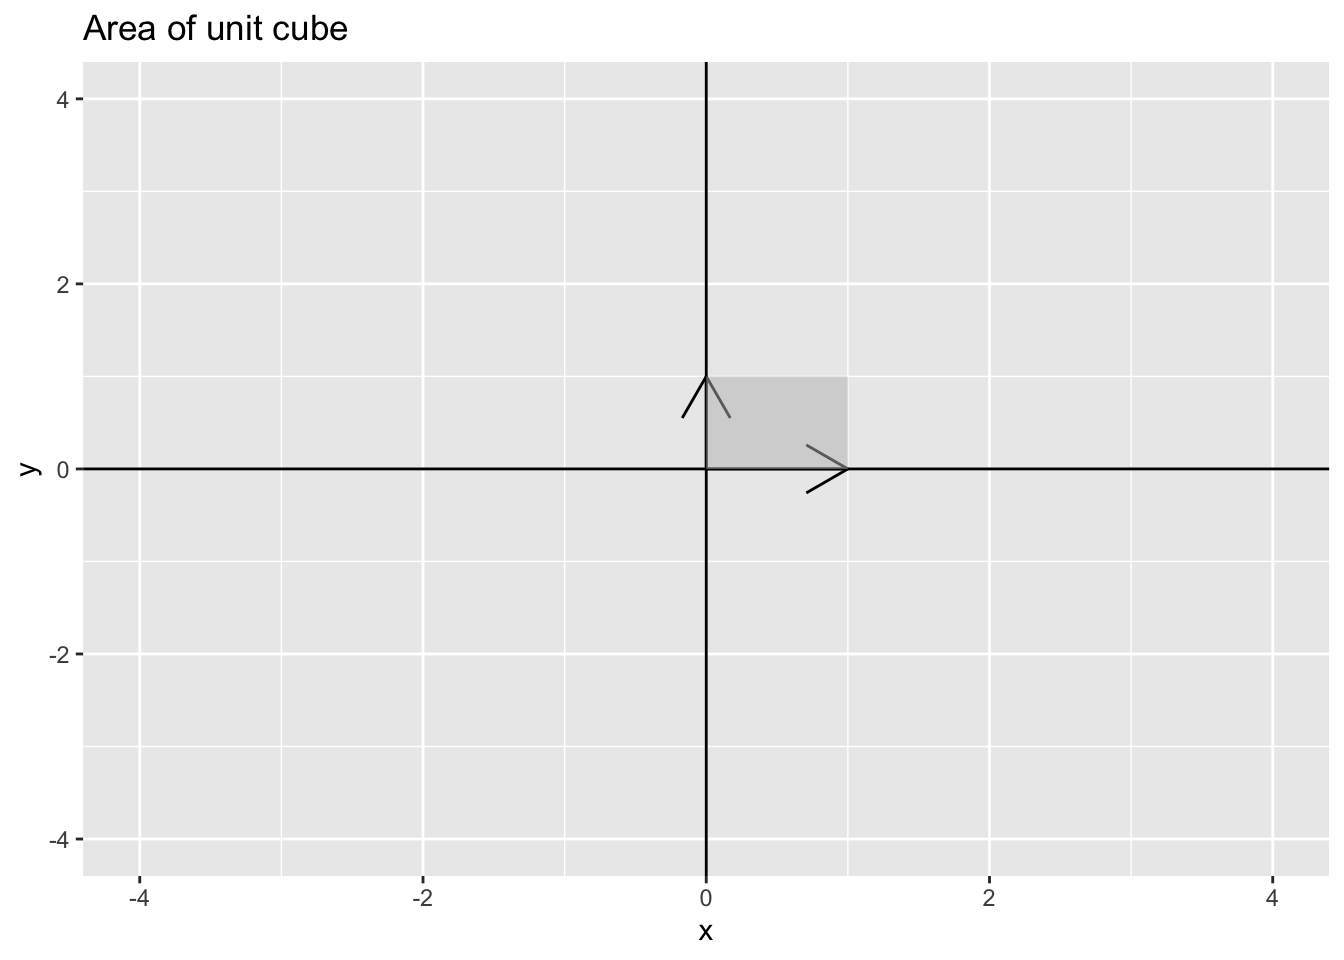
\includegraphics{multivariable-math_files/figure-latex/unnamed-chunk-156-1.pdf}

Which implies that if \(\mathbf{A} = \begin{pmatrix} 1 & 0 \\ 0 & 1 \end{pmatrix}\) has \(\det(\mathbf{A}) = 1\) because \(\mathbf{A} = \mathbf{I}\) the identity matrix.

\begin{Shaded}
\begin{Highlighting}[]
\KeywordTok{det}\NormalTok{(}\KeywordTok{matrix}\NormalTok{(}\KeywordTok{c}\NormalTok{(}\DecValTok{1}\NormalTok{, }\DecValTok{0}\NormalTok{, }\DecValTok{0}\NormalTok{, }\DecValTok{1}\NormalTok{), }\DecValTok{2}\NormalTok{, }\DecValTok{2}\NormalTok{))}
\end{Highlighting}
\end{Shaded}

\begin{verbatim}
## [1] 1
\end{verbatim}

\end{example}

\begin{example}

parallelograms in \(\mathcal{R}^2\): A larger square

\begin{Shaded}
\begin{Highlighting}[]
\NormalTok{df_vector <-}\StringTok{ }\KeywordTok{data.frame}\NormalTok{(}\DataTypeTok{x =} \KeywordTok{c}\NormalTok{(}\DecValTok{2}\NormalTok{, }\DecValTok{0}\NormalTok{), }\DataTypeTok{y =} \KeywordTok{c}\NormalTok{(}\DecValTok{0}\NormalTok{, }\DecValTok{2}\NormalTok{))}
\NormalTok{df_polygon <-}\StringTok{ }\KeywordTok{data.frame}\NormalTok{(}\DataTypeTok{x =} \KeywordTok{c}\NormalTok{(}\DecValTok{0}\NormalTok{, }\DecValTok{2}\NormalTok{, }\DecValTok{2}\NormalTok{, }\DecValTok{0}\NormalTok{), }\DataTypeTok{y =} \KeywordTok{c}\NormalTok{(}\DecValTok{0}\NormalTok{, }\DecValTok{0}\NormalTok{, }\DecValTok{2}\NormalTok{, }\DecValTok{2}\NormalTok{))}
\NormalTok{p1 <-}\StringTok{ }\KeywordTok{ggplot}\NormalTok{() }\OperatorTok{+}
\StringTok{    }\KeywordTok{geom_segment}\NormalTok{(}\KeywordTok{aes}\NormalTok{(}\DataTypeTok{x =} \DecValTok{0}\NormalTok{, }\DataTypeTok{xend =}\NormalTok{ df_vector}\OperatorTok{$}\NormalTok{x[}\DecValTok{1}\NormalTok{], }\DataTypeTok{y =} \DecValTok{0}\NormalTok{, }\DataTypeTok{yend =}\NormalTok{ df_vector}\OperatorTok{$}\NormalTok{y[}\DecValTok{1}\NormalTok{]), }\DataTypeTok{arrow =} \KeywordTok{arrow}\NormalTok{()) }\OperatorTok{+}
\StringTok{    }\KeywordTok{geom_segment}\NormalTok{(}\KeywordTok{aes}\NormalTok{(}\DataTypeTok{x =} \DecValTok{0}\NormalTok{, }\DataTypeTok{xend =}\NormalTok{ df_vector}\OperatorTok{$}\NormalTok{x[}\DecValTok{2}\NormalTok{], }\DataTypeTok{y =} \DecValTok{0}\NormalTok{, }\DataTypeTok{yend =}\NormalTok{ df_vector}\OperatorTok{$}\NormalTok{y[}\DecValTok{2}\NormalTok{]), }\DataTypeTok{arrow =} \KeywordTok{arrow}\NormalTok{()) }\OperatorTok{+}
\StringTok{    }\KeywordTok{geom_vline}\NormalTok{(}\DataTypeTok{xintercept =} \DecValTok{0}\NormalTok{) }\OperatorTok{+}\StringTok{ }
\StringTok{    }\KeywordTok{geom_hline}\NormalTok{(}\DataTypeTok{yintercept =} \DecValTok{0}\NormalTok{) }\OperatorTok{+}
\StringTok{    }\KeywordTok{coord_cartesian}\NormalTok{(}\DataTypeTok{xlim =} \KeywordTok{c}\NormalTok{(}\OperatorTok{-}\DecValTok{4}\NormalTok{, }\DecValTok{4}\NormalTok{), }\DataTypeTok{ylim =} \KeywordTok{c}\NormalTok{(}\OperatorTok{-}\DecValTok{4}\NormalTok{, }\DecValTok{4}\NormalTok{)) }\OperatorTok{+}\StringTok{ }
\StringTok{    }\KeywordTok{geom_polygon}\NormalTok{(}\DataTypeTok{data =}\NormalTok{ df_polygon, }\KeywordTok{aes}\NormalTok{(}\DataTypeTok{x =}\NormalTok{ x, }\DataTypeTok{y =}\NormalTok{ y), }
                 \DataTypeTok{fill =} \StringTok{"grey"}\NormalTok{, }\DataTypeTok{alpha =} \FloatTok{0.5}\NormalTok{) }\OperatorTok{+}
\StringTok{    }\KeywordTok{ggtitle}\NormalTok{(}\StringTok{"Area of unit cube"}\NormalTok{)}
\NormalTok{p1}
\end{Highlighting}
\end{Shaded}

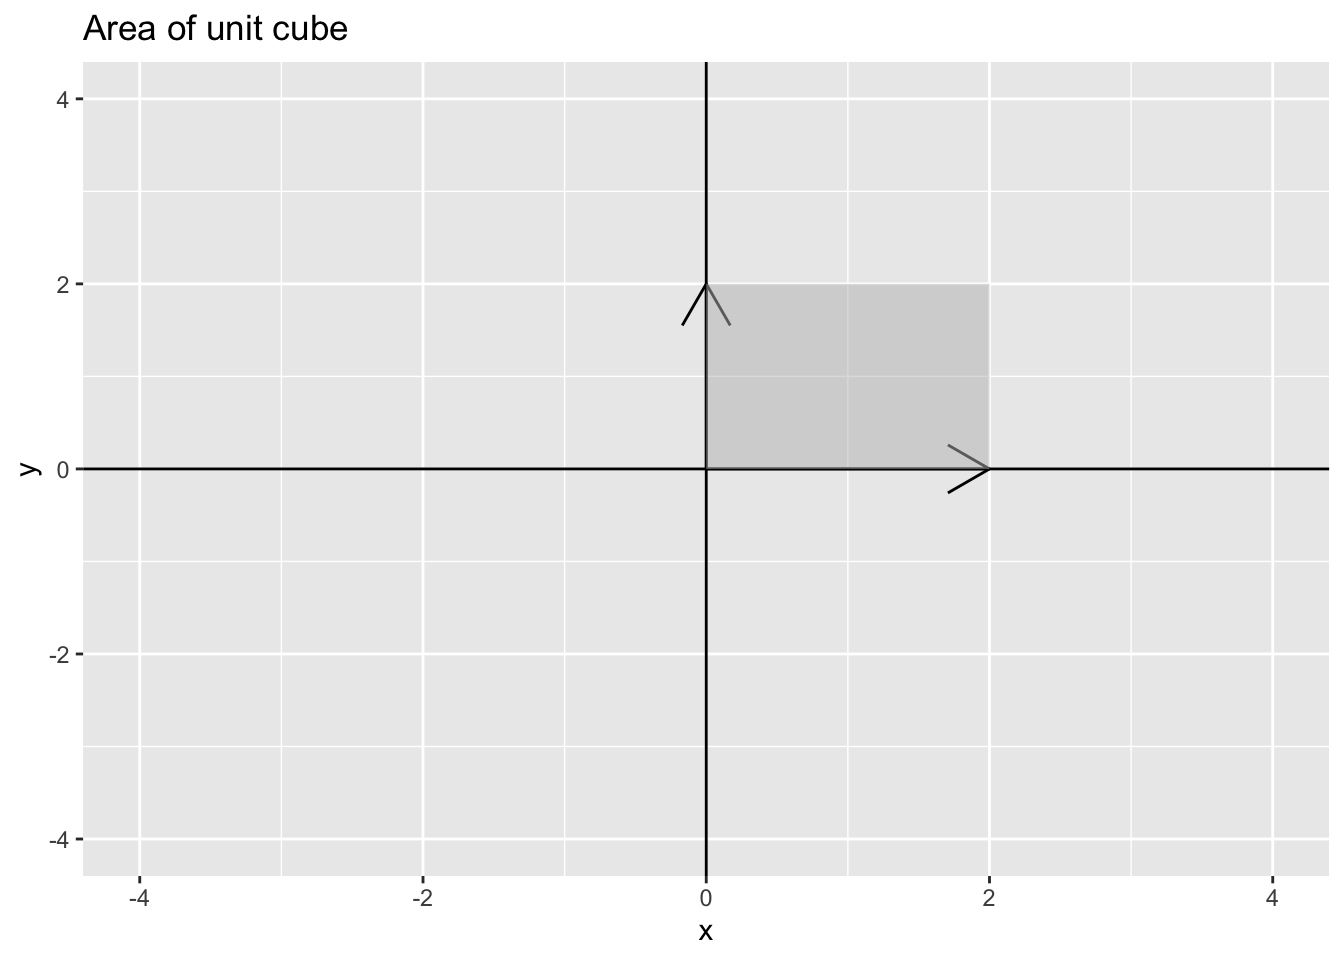
\includegraphics{multivariable-math_files/figure-latex/unnamed-chunk-158-1.pdf}

Which implies that if \(\mathbf{A} = \begin{pmatrix} 2 & 0 \\ 0 & 2 \end{pmatrix}\) has \(\det(\mathbf{A}) = 4\) because \(\mathbf{A} = 2 \mathbf{I}\) and the rule is for a constant \(c, \det(c\mathbf{A}) = c^n \det(\mathbf{A})\)

\begin{Shaded}
\begin{Highlighting}[]
\KeywordTok{det}\NormalTok{(}\KeywordTok{matrix}\NormalTok{(}\KeywordTok{c}\NormalTok{(}\DecValTok{2}\NormalTok{, }\DecValTok{0}\NormalTok{, }\DecValTok{0}\NormalTok{, }\DecValTok{2}\NormalTok{), }\DecValTok{2}\NormalTok{, }\DecValTok{2}\NormalTok{))}
\end{Highlighting}
\end{Shaded}

\begin{verbatim}
## [1] 4
\end{verbatim}

\end{example}

The Shiny app below allows you to plot the vector for any \((x, y)\) pair of your choosing.

\begin{Shaded}
\begin{Highlighting}[]
\KeywordTok{library}\NormalTok{(shiny)}
\KeywordTok{runGitHub}\NormalTok{(}\DataTypeTok{rep =} \StringTok{"multivariable-math"}\NormalTok{,}
          \DataTypeTok{username =} \StringTok{"jtipton25"}\NormalTok{,}
          \DataTypeTok{subdir =} \StringTok{"shiny-apps/chapter-14/determinants-volume/"}\NormalTok{) }
\end{Highlighting}
\end{Shaded}

\begin{theorem}[Determinants and Volume]
Let \(\mathbf{a}_1, \mathbf{a}_2, \ldots, \mathbf{a}_n\) be vectors in \(\mathcal{R}^n\), let \(\mathcal{P}\) be the parallelpiped determined by these vectors, and let \(\mathbf{A}\) be the matrix with columns \(\mathbf{a}_1, \mathbf{a}_2, \ldots, \mathbf{a}_n\). Then, the absolute value of the determinant of \(\mathbf{A}\) is the volume of the parallelpiped \(\mathcal{P}\):

\[
\begin{aligned}
|\det(\mathbf{A})| = \operatorname{volume}(\mathcal{P})
\end{aligned}
\]
\end{theorem}

\begin{proof}
Recall the 4 defining properties (Definition \ref{def:determinant}) that characterize the determinant. These properties also characterize the absolute value of the determinant.

From the 4 defining properties, the absolute value of the determinant \(|\det|\) is a function on square \(n \times n\) matrices that satisfies the properties

\begin{enumerate}
\def\labelenumi{\alph{enumi})}
\item
  Row replacement (e.g., row i = row i + c * row j) of \(\mathbf{A}\) does not change \(|\det(\mathbf{A})|\)
\item
  Scaling a row of \(\mathbf{A}\) by a scalar \(c\) changes \(|\det(\mathbf{A})|\) by multiplication by \(|c|\)
\item
  Swapping two rows of \(\mathbf{A}\) does not change \(|\det(\mathbf{A})|\)
\item
  The determinant of the identity matrix \(\mathbf{I}\) is 1
\end{enumerate}

Like the determinant and its 4 defining characteristics (Definition \ref{def:determinant}), the absolute value of the determinant is the only function that satisfies this relationship. Define \(vol(\mathcal{P}_A)\) as the volume of the parallelpiped defined by the rows of the square matrix \(\mathbf{A}\). In what follows, we will show that \(vol(\mathcal{P}_A)\) also satisfies the 4 defining characteristics of the absolute value of the determinant and, by the uniqueness of the function of the absolute value of the determinant, is equivalent to the absolute value of the determinant.

c) We start with showing that row swaps have no impact of the volume of the parallelpiped. Swapping two rows of \(\mathbf{A}\) just reorders the vectors \(\mathbf{a}_1, \mathbf{a}_2, \ldots, \mathbf{a}_n\) and the order has no impact of the calculation of the volume (e.g., area in 2d = length * width = width * length)

a) Consider a row replacement of \(\mathbf{a}_i \leftarrow \mathbf{a}_i + c \mathbf{a}_j\) for some \(j \neq i\). Because reordering has no effect on the volume of the parallelpiped, assume WLOG (without loss of generality--fancy math speak for this one case works for all the other possible cases) that we are replacing the last row (\(\mathbf{a}_n \leftarrow \mathbf{a}_n + c \mathbf{a}_j\)). Then, the area of the parallelpiped is defined as the base times the height. Let the ``base'' be the set of vectors \(\mathbf{a}_1, \mathbf{a}_2, \ldots \mathbf{a}_{n-1}\) which are the same for the original matrix and the row-replaced matrix. Therefore, if there is a difference in volume of the parallelpiped, it must be due to a difference in height. By definition, \(\mathbf{a}_j \in \operatorname{span}\{\mathbf{a}_1, \mathbf{a}_2, \ldots, \mathbf{a}_{n-1}\}\) so \(c \mathbf{a}_j\) is a vector that points in the same direction as the ``base'' which implies that translation of \(\mathbf{a}_n\) by \(c \mathbf{a}_j\) is parallel to the ``base''. As this is a parallel translation, the distance from the ``base'' to \(\mathbf{a}_n\) must be equal to the distance from the ``base'' to \(\mathbf{a}_n + c \mathbf{a}_j\) (the definition of parallel) which means the height is unchanged and therefore the volume of \(vol(\mathcal{P}_A)\) is unchanged by row replacement.

\textbf{Draw an example here}

b) WLOG assume we are scaling the last row \(\mathbf{a}_n\) (we can always swap rows without changing volume so this is ok). Scaling \(\mathbf{a}_n\) by a scalar \(c\) leaves the ``base'' of the parallelpiped unchanged (the ``base'' is defined as \(\mathbf{a}_1, \mathbf{a}_2, \ldots, \mathbf{a}_{n-1}\) which are unchanged). Therefore, the only question is whether the height from the base is changed when scaling \(\mathbf{a}_n\) by \(|c|\). In fact, scaling the vector \(\mathbf{a}_n\) by \(|c|\) changes the height by \(|c|\) and therefore the volume \(vol(\mathcal{P}_A)\) is scaled by \(|c|\).

\textbf{Draw an example in class}

d) The identity matrix having volume 1 is easy. The vectors of the identity matrix \(\mathbf{I}\) define a unit cube (technically a hypercube) which has area equal to the product of the lengths of each of their sides, which are each 1.

Because the absolute value of the determinant \(|\det|\) is the only function that satisfies, these properties, we have

\[
\begin{aligned}
vol(\mathcal{P}_A) = |\det(\mathbf{A})|
\end{aligned}
\]
\end{proof}

\textbf{Note:} Because \(\det(\mathbf{A}) = \det(\mathbf{A}')\), the absolute value of the determinant is equal to the volume of the parallelpiped defined by the columns of \(\mathbf{A}\) (we could just have easily done all the calculations on the columns of \(\mathbf{A}\) as the rows of \(\mathbf{A}\)).

\begin{example}
1 by 1 matrix \(a\) (length) has \(\det(a) = a\)
\end{example}

\begin{example}
2 by 2 matrix \(\begin{pmatrix} a & c \\ b & d \end{pmatrix}\)
\end{example}

\begin{example}
Find the area of a parallelogram with sides defined by the vectors \(\begin{pmatrix} 2 \\ 4 \end{pmatrix}\) and \(\begin{pmatrix} -1 \\ 2 \end{pmatrix}\)
\end{example}

area of a triangle -- choose two sides and find area of parallelogram and divide by 2

\begin{example}
Recall that in data science, a probability distribution is function that has volume under the surface of one. For common distributions, particularly the normal/Gaussian distribution, the determinant is the factor that scales the function so that the volume under the surface is one.

The vector \(\mathbf{y}\) is said to have a multivariate normal distribution with mean \(\boldsymbol{\mu}\) and covariance matrix \(\boldsymbol{\Sigma}\) if the probability density function of \(\mathbf{y}\) is
\[
\begin{aligned}
f(\mathbf{y}) = (2 \pi)^{-n/2} |\det(\boldsymbol{\Sigma})|^{-1/2} e^{- \frac{1}{2} (\mathbf{y} - \boldsymbol{\mu})' \boldsymbol{\Sigma}^{-1} (\mathbf{y} - \boldsymbol{\mu})}
\end{aligned}
\]

Notice in this equation that the determinant \(\det(\boldsymbol{\Sigma})\) plays a key role in the definition of the probability distribution. This is because

\[\begin{aligned}
\int_{\mathbf{y}} (2 \pi)^{-n/2} e^{- \frac{1}{2} (\mathbf{y} - \boldsymbol{\mu})' \boldsymbol{\Sigma}^{-1} (\mathbf{y} - \boldsymbol{\mu})} \, d\mathbf{y} = |\det(\boldsymbol{\Sigma})|^{1/2}
\end{aligned}
\]
which implies that
\[
\begin{aligned}
\frac{\int_{\mathbf{y}} (2 \pi)^{-n/2} e^{- \frac{1}{2} (\mathbf{y} - \boldsymbol{\mu})' \boldsymbol{\Sigma}^{-1} (\mathbf{y} - \boldsymbol{\mu})} \, d\mathbf{y}}{|\det(\boldsymbol{\Sigma})|^{1/2}} = 1
\end{aligned}
\]

In probability and statistics, the denominator is known as the \href{https://en.wikipedia.org/wiki/Normalizing_constant}{``normalizing constant.''}
\end{example}

\hypertarget{volumes-of-parallelpipeds}{%
\section{Volumes of Parallelpipeds}\label{volumes-of-parallelpipeds}}

\begin{proposition}
Let \(\mathbf{a}_1\) and \(\mathbf{a}_2\) be nonzero vectors. Then, for any scalar \(c\), the area of the parallelpiped defined by \(\mathbf{a}_1\) and \(\mathbf{a}_2\) is the same as the area of the parallelpiped defined by the vectors \(\mathbf{a}_1\) and \(\mathbf{a}_2 + c \mathbf{a}_1\) (an elementary column operation).
\end{proposition}

\begin{example}
Draw a parallelpiped in class. Recall that areas of a parallelpiped are defined (in 2 dimensions) as the length of the base times the height perpindicular to the base. In 3 dimensions, the volume of a parallelpiped is the base times the width (the area of the base) times the height.
\end{example}

\hypertarget{volumes-of-linear-transformations}{%
\section{Volumes of Linear Transformations}\label{volumes-of-linear-transformations}}

Recall linear transformations \(T:\mathcal{R}^n \rightarrow \mathcal{R}^n\) (Section \ref{linear-transformations}) where for any \(\mathbf{x} \in \mathcal{R}^n\) (the domain), \(T(\mathbf{x}) = \mathbf{A} \mathbf{x} \in \mathcal{R}^n\) (the codomain).

\begin{theorem}
Let \(\mathcal{S}\) be a set in the domain that has a volume \(vol(\mathcal{S})\). Then, the volume of the image of the set under the transformation \(T(\mathcal{S})\) is \(vol(T(\mathcal{S})) = |\det(\mathbf{A})|vol(\mathcal{S})\)
\end{theorem}

\hypertarget{vector-spaces-and-subspaces}{%
\chapter{Vector Spaces and Subspaces}\label{vector-spaces-and-subspaces}}

\begin{itemize}
\tightlist
\item
  \href{https://www.3blue1brown.com/lessons/abstract-vector-spaces}{3 Blue 1 Brown -- Abstract vector spaces}
\end{itemize}

Recall the definition of a subspace:

\begin{definition}

A subspace \(\mathcal{H}\) of a vector space \(\mathcal{V}\) is a subset of \(\mathcal{V}\) such that

\begin{itemize}
\item
  \(\mathcal{H}\) contains the zero vector -- \(\mathbf{0} \in \mathcal{H}\)
\item
  \(\mathcal{H}\) is closed under vector addition. Therefore, for \(\mathbf{u}\) and \(\mathbf{v}\) in \(\mathcal{H}\), the sum \(\mathbf{u} + \mathbf{v}\) is in \(\mathcal{H}\)
\item
  \(\mathcal{H}\) is closed under scalar multiplication. Therefore, for \(\mathbf{u}\) in \(\mathcal{H}\) and a scalar \(a\), the product \(a \mathbf{u}\) is in \(\mathcal{H}\)
\end{itemize}

\end{definition}

A consequence of this definition is that a subspace \(\mathcal{H}\) is closed under linear combinations.

\hypertarget{null-space-and-column-space}{%
\section{Null space and column space}\label{null-space-and-column-space}}

Also, recall the special subspaces of the column space and the null space.

\hypertarget{null-space}{%
\subsection{Null space}\label{null-space}}

\begin{definition}
The null space null(\(\mathbf{A}\)) of an \(m \times n\) \(\mathbf{A}\) is the set of all solutions of the homogeneous equation \(\mathbf{A} \mathbf{x} = \mathbf{0}\)

Another way to write null(\(\mathbf{A}\)) is
\[
\begin{aligned}
\mbox{null}(\mathbf{A}) = \{\mathbf{x} : \mathbf{x} \in \mathcal{R}^n \mbox{ and } \mathbf{A} \mathbf{x} = \mathbf{0} \}
\end{aligned}
\]
\end{definition}

\begin{theorem}
The null space of an \(m \times n\) matrix \(\mathbf{A}\) is a subspace of \(\mathcal{R}^n\).
\end{theorem}

\begin{proof}
To show that the null space of \(\mathbf{A}\), denoted null(\(\mathbf{A})\), is a subspace we need to show the following

\begin{enumerate}
\def\labelenumi{\arabic{enumi})}
\item
  The zero vector \(\mathbf{0}\) is in the null space of \(\mathbf{A}\)
\item
  The null space of \(\mathbf{A}\) is closed under addition
\item
  The null space of \(\mathbf{A}\) is closed under scalar multiplication
\end{enumerate}

The null space of \(\mathbf{A}\) is defined as the set of vectors \(\mathbf{x}\) such that \(\mathbf{A} \mathbf{x} = \mathbf{0}\).

\begin{enumerate}
\def\labelenumi{\arabic{enumi})}
\item
  First, we show that the zero vector is in the subspace by setting \(\mathbf{x} = \mathbf{0}\). Thus, because \(\mathbf{A} \mathbf{0} = \mathbf{0}\), the zero vector \(\mathbf{0}\) is in the null space of \(\mathbf{A}\) .
\item
  Next, let \(\mathbf{u}\) and \(\mathbf{v}\) be vectors in the null space of \(\mathbf{A}\). Thus, by the definition of the null space we have \(\mathbf{A} \mathbf{u} = \mathbf{0}\) and \(\mathbf{A} \mathbf{v} = \mathbf{0}\). Consider the vector \(\mathbf{u} + \mathbf{v}\) and consider \(\mathbf{A} (\mathbf{u} + \mathbf{v}) = \mathbf{A} \mathbf{u} + \mathbf{A} \mathbf{v} = \mathbf{0} + \mathbf{0} = \mathbf{0}\). Thus \(\mathbf{u} + \mathbf{v}\) is in the null space of \(\mathbf{A}\).
\item
  Finally, let \(\mathbf{u}\) be a vector in the null space of \(\mathbf{A}\) and let \(c\) be a scalar. Thus, by the definition of the null space we have \(\mathbf{A} \mathbf{u} = \mathbf{0}\). Then, consider \(\mathbf{A} (c \mathbf{u}) = c \mathbf{A} \mathbf{u} = c \mathbf{0} = \mathbf{0}\)
\end{enumerate}

Because the three requirements for a subspace are met, this gives us that the null space of \(\mathbf{A}\) is a subspace.
\end{proof}

As a consequence, there will exist a set of vectors that span the null space null(\(\mathbf{A}\)). However, the null space of \(\mathbf{A}\) is defined implicitly. This means that the null space of \(\mathbf{A}\) is not obvious given the vectors of \(\mathbf{A}\) and must be checked/calculated.

\begin{example}

\begin{itemize}
\tightlist
\item
  In class
\end{itemize}

Find a spanning set for null(\(\mathbf{A}\)) where

\[
\begin{aligned}
\mathbf{A} = \begin{pmatrix} 7 & -2 & 7 & -4 & 5 \\ 2 & 0 & 3 & 3 & 9 \\ -5 & 2 & -5 & 7 & -2 \end{pmatrix}
\end{aligned}
\]

\begin{itemize}
\tightlist
\item
  Find solution to system of homogeneous system of equations \(\mathbf{A} \mathbf{x} = \mathbf{0}\)
\end{itemize}

\begin{Shaded}
\begin{Highlighting}[]
\NormalTok{A <-}\StringTok{ }\KeywordTok{matrix}\NormalTok{(}\KeywordTok{c}\NormalTok{(}\DecValTok{7}\NormalTok{, }\DecValTok{2}\NormalTok{, }\DecValTok{-5}\NormalTok{, }\DecValTok{-2}\NormalTok{, }\DecValTok{0}\NormalTok{, }\DecValTok{2}\NormalTok{, }\DecValTok{7}\NormalTok{, }\DecValTok{3}\NormalTok{, }\DecValTok{-5}\NormalTok{, }\DecValTok{-4}\NormalTok{, }\DecValTok{3}\NormalTok{, }\DecValTok{7}\NormalTok{, }\DecValTok{5}\NormalTok{, }\DecValTok{9}\NormalTok{, }\DecValTok{-2}\NormalTok{), }\DecValTok{3}\NormalTok{, }\DecValTok{5}\NormalTok{)}
\KeywordTok{rref}\NormalTok{(}\KeywordTok{cbind}\NormalTok{(A, }\DecValTok{0}\NormalTok{))}
\end{Highlighting}
\end{Shaded}

\begin{verbatim}
##      [,1] [,2] [,3] [,4]  [,5] [,6]
## [1,]    1    0    0 1.50 -4.50    0
## [2,]    0    1    0 7.25  2.75    0
## [3,]    0    0    1 0.00  6.00    0
\end{verbatim}

\begin{itemize}
\item
  Take the general solution and write as a linear combination of vectors where the coefficients are the free variables.
\item
  general solution \(x_1 = -1.5 x_4 + 4.5 x_5\), \(x_2 = -7.25 x_4 - 2.75 x_5\), \(x_3 = -6 x_5\) and both \(x_4\) and \(x_5\) are free. Write out the general solution in vector form.
\end{itemize}

\[
\begin{aligned}
\begin{pmatrix} x_1 \\ x_2 \\ x_3 \\ x_4 \\ x_5 \end{pmatrix} = \begin{pmatrix} -1.5 x_4 + 4.5 x_5\\ -7.25 x_4 - 2.75 x_5 \\ -6 x_5 \\ x_4 \\ x_5 \end{pmatrix} = x_4 \begin{pmatrix} -1.5 \\ -7.25 \\ 0 \\ 1 \\ 0 \end{pmatrix} + x_5 \begin{pmatrix} 4.5 \\ 2.75 \\ -6 \\ 0 \\ 1 \end{pmatrix}
\end{aligned}
\]

\begin{itemize}
\tightlist
\item
  From above, the free variables \(x_4\) and \(x_5\) are multiplied by the vectors \(\mathbf{u} = \begin{pmatrix} -1.5 \\ -7.25 \\ 0 \\ 1 \\ 0 \end{pmatrix}\) and \(\mathbf{v} = \begin{pmatrix} 4.5 \\ 2.75 \\ -6 \\ 0 \\ 1 \end{pmatrix}\) where \(\{ \mathbf{u}, \mathbf{v} \}\) are a spanning set for the null(\(\mathbf{A}\))
\end{itemize}

\end{example}

\begin{example}

\begin{itemize}
\tightlist
\item
  In class -- do another
  Find a spanning set for null(\(\mathbf{A}\)) where
\end{itemize}

\end{example}

\hypertarget{column-space}{%
\subsection{Column space}\label{column-space}}

\begin{definition}
The columns space col(\(\mathbf{A}\)) of an \(m \times n\) \(\mathbf{A}\) is the set of all linear combinations of the columns of \(\mathbf{A}\).

If \(\{ \mathbf{a}_1, \ldots, \mathbf{a}_n\}\) are the columns of \(\mathbf{A}\), then
\[
\begin{aligned}
\mbox{col}(\mathbf{A}) = \mbox{span}(\mathbf{A})
\end{aligned}
\]
this can be written in set notation as
\[
\begin{aligned}
\mbox{col}(\mathbf{A}) = \{ \mathbf{b} : \mathbf{A} \mathbf{x} = \mathbf{b} \mbox{ for some } \mathbf{x} \in \mathcal{R}^n \}
\end{aligned}
\]
\end{definition}

\begin{theorem}
The column space of an \(m \times n\) matrix \(\mathbf{A}\) is a subspace of \(\mathcal{R}^n\).
\end{theorem}

\begin{proof}

Do in class

\begin{itemize}
\item
  \(\mathbf{0}\) vector
\item
  sum of vectors
\item
  scalar multiplication
\end{itemize}

\end{proof}

Compared to the null space, the column space is defined explicitly--it is the span of the columns of \(\mathbf{A}\). The definition of the column space results in the fact that col(\(\mathbf{A}\)) is the range of the linear transformation \(\mathbf{x} \rightarrow \mathbf{A} \mathbf{x}\).

\begin{example}

\begin{itemize}
\tightlist
\item
  In class
\end{itemize}

Find a spanning set for col(\(\mathbf{A}\)) where

\[
\begin{aligned}
\mathbf{A} = \begin{pmatrix} 6 & 0 & 4 \\ 5 & -1 & -9 \\ -4 & 7 & 4 \\ 6 & 2 & 9 \end{pmatrix}
\end{aligned}
\]

\end{example}

\hypertarget{understanding-the-differerneces-between-the-column-space-and-the-null-space}{%
\subsection{Understanding the differerneces between the column space and the null space}\label{understanding-the-differerneces-between-the-column-space-and-the-null-space}}

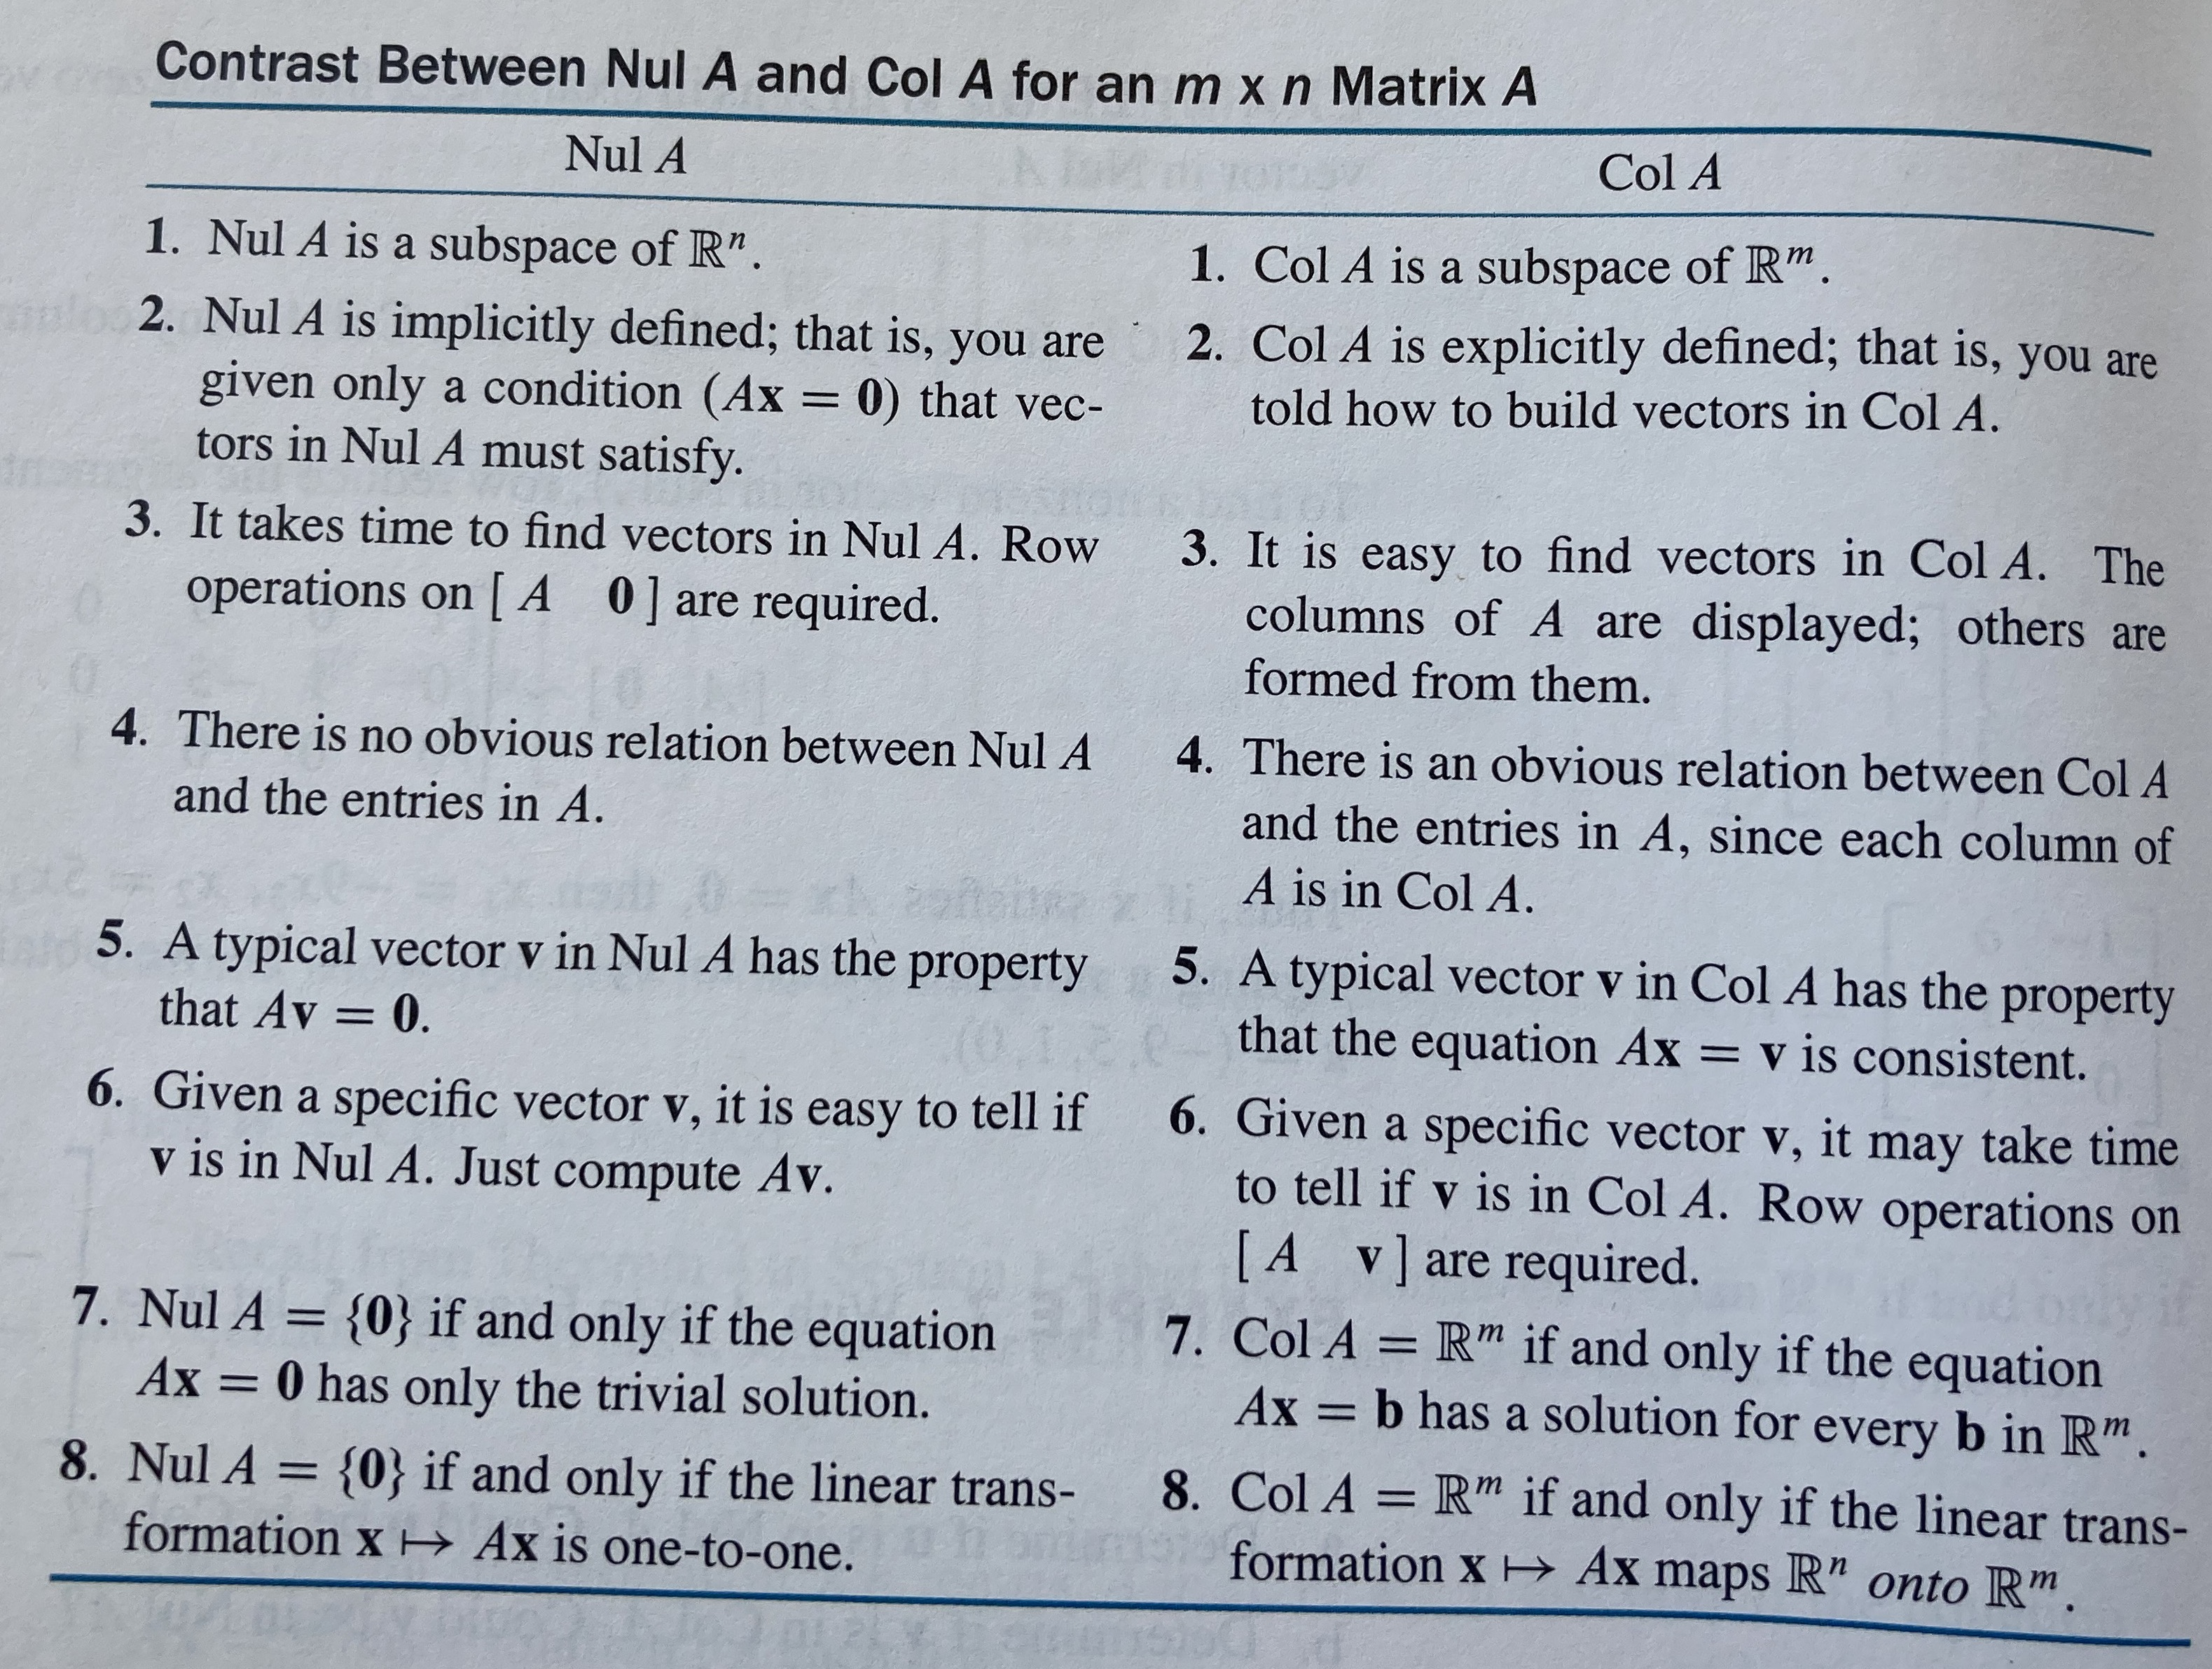
\includegraphics[width=1\linewidth]{/Users/runner/work/multivariable-math/multivariable-math/images/null-column}

\hypertarget{linearly-independent-sets-and-bases}{%
\chapter{Linearly independent sets and bases}\label{linearly-independent-sets-and-bases}}

\begin{Shaded}
\begin{Highlighting}[]
\KeywordTok{library}\NormalTok{(tidyverse)}
\KeywordTok{library}\NormalTok{(dasc2594)}
\end{Highlighting}
\end{Shaded}

Recall that a set of vectors \(\{ \mathbf{v}_1, \ldots, \mathbf{v}_n\}\) is linearly independent if the only solution to the system of equations

\[
\begin{aligned}
x_1 \mathbf{v}_1 + \cdots + x_n \mathbf{v}_n = \mathbf{0}
\end{aligned}
\]
is the trivial solution \(\mathbf{x} = \mathbf{0}\). In other words, it is not possible to write any of the vectors in the set \(\{ \mathbf{v}_1, \ldots, \mathbf{v}_n\}\) as a linear combination of the other vectors.

\begin{definition}

Let \(\mathcal{H}\) be a subspace of a vector space \(\mathcal{V}\). Then, the set of vectors \(\mathcal{B} = \{ \mathbf{v}_1, \ldots, \mathbf{v}_n \}\) is a \textbf{basis} for \(\mathcal{H}\) if

\begin{itemize}
\item
  The set of vectors \(\mathcal{B}\) are linearly independent
\item
  The subspace spanned by \(\mathcal{B}\) is \(\mathcal{H}\). In other words
  \[
  \begin{aligned}
  \mbox{span}(\mathbf{v}_1, \ldots, \mathbf{v}_n) = \mathcal{H}
  \end{aligned}
  \]
\end{itemize}

\end{definition}

\begin{example}

\begin{itemize}
\tightlist
\item
  in class--standard basis \(\mathbf{e}_1, \ldots \mathbf{e}_n\) which are the columns of the \(n \times n\) identity matrix\(\mathbf{I}\).
\end{itemize}

\end{example}

\begin{example}

\begin{itemize}
\tightlist
\item
  in class--pick 3 vectors of length 3. Are they a basis for \(\mathcal{R}^3\)? What about \(\mathcal{R}^4\)?
\end{itemize}

\end{example}

\begin{theorem}[The Spanning Set Theorem]

Let \(\mathcal{S} = \{\mathbf{v}_1, \ldots, \mathbf{v}_n\}\) be vectors in the vector space \(\mathcal{V}\) and let \(\mathcal{H}\) = span(\(\mathbf{v}_1, \ldots, \mathbf{v}_n\))

\begin{enumerate}
\def\labelenumi{\alph{enumi})}
\item
  If one of the vectors, say \(\mathbf{v}_k\), of \(\mathcal{S}\) is a linear combination of the remaining vectors of \(\mathcal{S}\), then the set formed by removing the vector \(\mathbf{v}_k\) still spans \(\mathcal{H}\)
\item
  If \(\mathcal{H} \neq \{\mathbf{0}\}\), then some subset of \(\mathcal{S}\) spans \(\mathcal{H}\).
\end{enumerate}

\end{theorem}

\begin{proof}

We will show the proof for bot parts (a) and (b) of the theroem

\begin{enumerate}
\def\labelenumi{\alph{enumi})}
\item
  WLOG assume \(\mathbf{v}_n\) is a linear combination of \(\mathbf{v}_1, \ldots, \mathbf{v}_{n-1}\) (if not, permute the labels to make the linearly dependent vector the \(n\)th vector). Then
  \[
  \begin{aligned}
  \mathbf{v}_n = x_1 \mathbf{v}_1 + \cdots + x_{n-1} \mathbf{v}_{n-1}
  \end{aligned}
  \label{eq:span-set-theorem1}
  \]
  Because the vectors \(\{\mathbf{v}_1, \ldots, \mathbf{v}_n\}\) span \(\mathcal{H}\), any vector \(\mathbf{b}\in \mathcal{H}\) can be written as
  \[
  \begin{aligned}
  \mathbf{b} = c_1 \mathbf{v}_1 + \cdots + c_{n} \mathbf{v}_{n}
  \end{aligned}
  \label{eq:span-set-theorem2}
  \]\\
  for scalars \(c_1, \ldots, c_n\). Plugging the result from \eqref{eq:span-set-theorem1} into \eqref{eq:span-set-theorem2} shows that any vector \(\mathbf{b}\) in \(\mathcal{H}\) can be written only using the vectors \(\mathbf{v}_1, \ldots, \mathbf{v}_{n-1}\)
\item
  As the vectors in \(\mathcal{S}\) span \(\mathcal{H}\), if there is a linearly dependent vector in \(\mathcal{S}\), this vector can be removed from \(\mathcal{S}\) and the span of this subset of \(\mathcal{S}\) will still span \(\mathcal{H}\). As long as \(\mathbf{H} \neq \{\mathbf{0}\}\), there must be a least one nonzero vector in \(\mathbf{S}\) so the removing of linearly dependent vectors will stop with at least one vector. As all of the linearly dependent vectors have been removed, the subset of \(\mathcal{S}\) created in this manner will be a set of linearly independent vectors that span \(\mathcal{H}\).
\end{enumerate}

\end{proof}

\hypertarget{bases-for-nullmathbfa-and-colmathbfa}{%
\section{\texorpdfstring{Bases for null(\(\mathbf{A}\)) and col(\(\mathbf{A}\))}{Bases for null(\textbackslash mathbf\{A\}) and col(\textbackslash mathbf\{A\})}}\label{bases-for-nullmathbfa-and-colmathbfa}}

\begin{example}

Find a basis for the col(\(\mathbf{A}\)) where

\begin{Shaded}
\begin{Highlighting}[]
\KeywordTok{set.seed}\NormalTok{(}\DecValTok{2021}\NormalTok{)}
\NormalTok{A <-}\StringTok{ }\KeywordTok{matrix}\NormalTok{(}\KeywordTok{sample}\NormalTok{(}\OperatorTok{-}\DecValTok{9}\OperatorTok{:}\DecValTok{9}\NormalTok{, }\DecValTok{15}\NormalTok{, }\DataTypeTok{replace =} \OtherTok{TRUE}\NormalTok{), }\DecValTok{5}\NormalTok{, }\DecValTok{3}\NormalTok{)}
\end{Highlighting}
\end{Shaded}

\[
\begin{aligned}
\mathbf{A} = \begin{pmatrix} -3 & -4 & 5 \\ -4 & -4 & -3 \\ 4 & -4 & -1 \\ -3 & 4 & 2 \\ 2 & -5 & 9 \end{pmatrix}
\end{aligned}
\]
* Calculate row echelon form and identify the pivot columns. The vectors \(\mathbf{a}_1, \ldots, \mathbf{a}_n\) that make up the columns of \(\mathbf{A}\) that are in the pivot columns form a basis for \(\mathbf{A}\)

\begin{itemize}
\tightlist
\item
  Why is this? Think about the relationship between the columns of \(\mathbf{A}\) and the vector \(\mathbf{b}\) in \(\mathbf{A} \mathbf{x} = \mathbf{b}\) that result in a consistent solution.
\end{itemize}

\end{example}

\begin{example}

Find a basis for the null(\(\mathbf{A}\)) where

\begin{Shaded}
\begin{Highlighting}[]
\KeywordTok{set.seed}\NormalTok{(}\DecValTok{2021}\NormalTok{)}
\NormalTok{A <-}\StringTok{ }\KeywordTok{matrix}\NormalTok{(}\KeywordTok{sample}\NormalTok{(}\OperatorTok{-}\DecValTok{9}\OperatorTok{:}\DecValTok{9}\NormalTok{, }\DecValTok{15}\NormalTok{, }\DataTypeTok{replace =} \OtherTok{TRUE}\NormalTok{), }\DecValTok{5}\NormalTok{, }\DecValTok{3}\NormalTok{)}
\end{Highlighting}
\end{Shaded}

\[
\begin{aligned}
\mathbf{A} = \begin{pmatrix} -3 & -4 & 5 \\ -4 & -4 & -3 \\ 4 & -4 & -1 \\ -3 & 4 & 2 \\ 2 & -5 & 9 \end{pmatrix}
\end{aligned}
\]

\begin{itemize}
\tightlist
\item
  Calculate solutions to homogeneous system of equations, write solution in vector equation form. Vectors form a basis for null(\(\mathbf{A}\))
\end{itemize}

\end{example}

\begin{itemize}
\tightlist
\item
  \textbf{note:} Facts about the basis for the null space null(\(\mathbf{A}\))
\end{itemize}

\begin{enumerate}
\def\labelenumi{\arabic{enumi})}
\item
  The spanning set produced using the method above produces a linearly independent set because the free variables are weights on the spanning vectors.
\item
  When null(\(\mathbf{A}\)) contains nonzero vectors, the number of vectors in the spanning set for null(\(\mathbf{A}\)) is the number of free variables in the solution of \(\mathbf{A} \mathbf{x} = \mathbf{0}\).
\end{enumerate}

\begin{example}
The matrix \(4 \times 5\) \(\mathbf{A}\) has columns given by the vectors \(\mathbf{a}_1, \ldots, \mathbf{a}_5\) and is row equivalent to the matrix
\[
\begin{aligned}
\mathbf{A} = \begin{pmatrix} 1 & 0 & 3 & -2 & 1 \\ 0 & 0 & 3 & -2 & 5 \\ 0 & 0 & 0 & -1 & -2 \\ 0 & 0 & 0 & 0 & 0 \end{pmatrix}
\end{aligned}
\]
What is a basis for col(\(\mathbf{A}\)) in terms of the vectors \(\mathbf{a}_1, \ldots, \mathbf{a}_5\)
\end{example}

\begin{itemize}
\tightlist
\item
  Note that two matrices that are row equivalent have the same linear dependence relationsihps between their vectors (but the basis for their column space is different)
\end{itemize}

\begin{example}

The matrix \(\mathbf{A}\) is row equivalent to the matrix \(\mathbf{B}\)

\begin{Shaded}
\begin{Highlighting}[]
\NormalTok{A <-}\StringTok{ }\KeywordTok{matrix}\NormalTok{(}\KeywordTok{c}\NormalTok{(}\DecValTok{1}\NormalTok{, }\DecValTok{3}\NormalTok{, }\DecValTok{2}\NormalTok{, }\DecValTok{5}\NormalTok{, }\DecValTok{4}\NormalTok{, }\DecValTok{12}\NormalTok{ , }\DecValTok{8}\NormalTok{, }\DecValTok{20}\NormalTok{, }\DecValTok{0}\NormalTok{, }\DecValTok{1}\NormalTok{, }\DecValTok{1}\NormalTok{, }\DecValTok{2}\NormalTok{, }\DecValTok{2}\NormalTok{, }\DecValTok{5}\NormalTok{, }\DecValTok{3}\NormalTok{, }\DecValTok{8}\NormalTok{, }\DecValTok{-1}\NormalTok{, }\DecValTok{5}\NormalTok{, }\DecValTok{2}\NormalTok{, }\DecValTok{8}\NormalTok{), }\DecValTok{4}\NormalTok{, }\DecValTok{5}\NormalTok{)}
\NormalTok{B <-}\StringTok{ }\KeywordTok{rref}\NormalTok{(A)}
\end{Highlighting}
\end{Shaded}

\[
\begin{aligned}
\mathbf{A} = \begin{pmatrix} 1 & 4 & 0 & 2 & -1 \\ 3 & 12 & 1 & 5 & 5 \\ 2 & 8 & 1 & 3 & 2 \\ 5 & 20 & 2 & 8 & 8 \end{pmatrix} & \mathbf{B} = \begin{pmatrix} 1 & 4 & 0 & 2 & 0 \\ 0 & 0 & 1 & -1 & 0 \\ 0 & 0 & 0 & 0 & 1 \\ 0 & 0 & 0 & 0 & 0 \end{pmatrix} \\
\end{aligned}
\]

\begin{itemize}
\item
  What is a basis for col(\(\mathbf{A}\))?
\item
  What is a basis for col(\(\mathbf{B}\))?
\item
  What is span(\(\mathbf{a}_1, \ldots, \mathbf{a}_5\))?
\item
  What is span(\(\mathbf{b}_1, \ldots, \mathbf{b}_5\))?
\item
  Are the spaces spanned by the columns of \(\mathbf{A}\) and the columns of \(\mathbf{B}\) the same space?
\end{itemize}

\end{example}

\begin{theorem}
The pivot columns of a matrix \(\mathbf{A}\) for a basis for col(\(\mathbf{A}\))
\end{theorem}

\begin{proof}
sketch: \(\mathbf{B}\) rref of \(\mathbf{A}\), linearly independent columns of \(\mathbf{B}\) are same as linearly independent columns in \(\mathbf{A}\). Other (non-pviot) columns are linearly dependent. By spanning set theorem, non-pivot columns can be removed from the spanning set without changing the span, leaving only the pivot columns of \(\mathbf{A}\) as a basis for col(\$)
\end{proof}

\hypertarget{coordinate-systems-and-dimension}{%
\chapter{Coordinate Systems and Dimension}\label{coordinate-systems-and-dimension}}

\begin{itemize}
\tightlist
\item
  \href{https://www.3blue1brown.com/lessons/change-of-basis}{3 Blue 1 Brown -- Change of basis}
\end{itemize}

\newcommand{\basis}{{\mathcal{B} = \{ \mathbf{b}_1, \ldots, \mathbf{b}_n \}}}
\newcommand{\V}{{\mathcal{V}}}

\begin{Shaded}
\begin{Highlighting}[]
\KeywordTok{library}\NormalTok{(tidyverse)}
\KeywordTok{library}\NormalTok{(dasc2594)}
\end{Highlighting}
\end{Shaded}

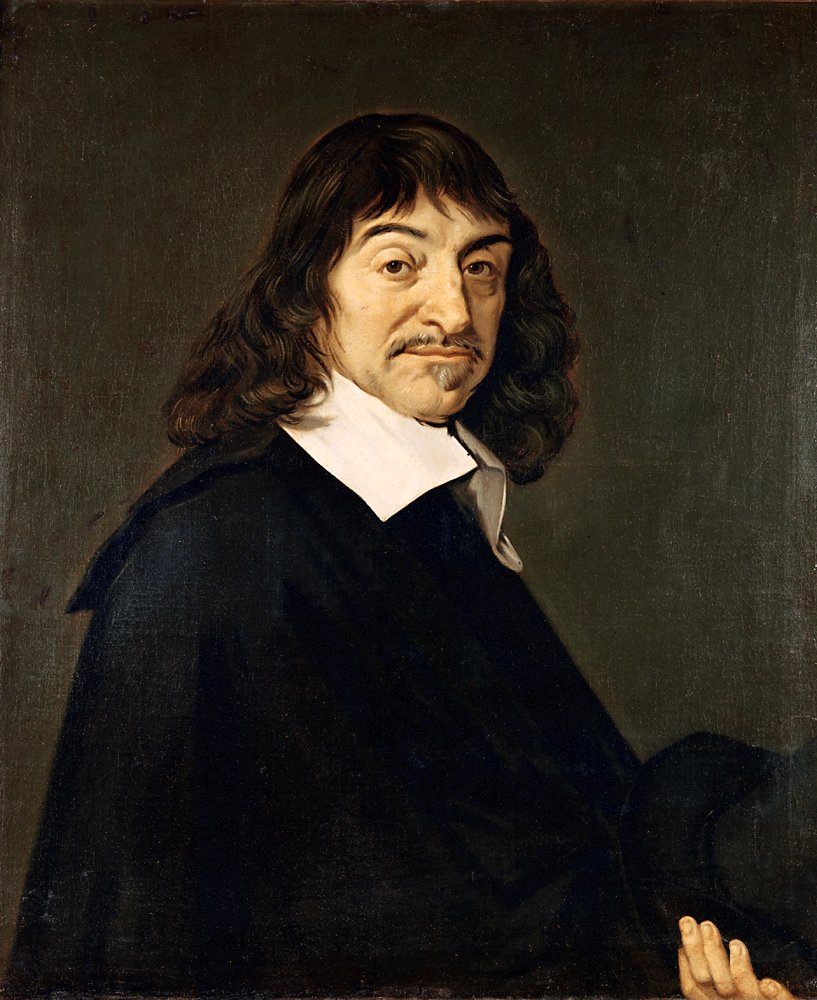
\includegraphics[width=1\linewidth]{/Users/runner/work/multivariable-math/multivariable-math/images/descartes}

We already know about the cartesian coordinate system (x, y, z) which has the set of basis vectors
\[
\begin{aligned}
\mathbf{e}_1 = \begin{pmatrix} 1 \\ 0 \\ 0 \end{pmatrix} && 
\mathbf{e}_2 = \begin{pmatrix} 0 \\ 1 \\ 0 \end{pmatrix} && 
\mathbf{e}_3 = \begin{pmatrix} 0 \\ 0 \\ 1 \end{pmatrix} 
\end{aligned}
\]

However, using the concept of a basis for a subspace \(\mathcal{H}\) of some vector space \(\mathcal{V}\), we might want to use a different basis. Luckily, we have learned how to construct bases for col(\(\mathbf{A}\)) and null(\(\mathbf{A}\)).

You might be wondering why we want to create different bases. The usual cartesian basis has been good enough for me so far (unless you have used polar coordinates). In data science, the data often live in a high dimensional space (i.e., there are a number of data variables). However, while the data might have many variables, some of these variables are partially dependent and thus the space in which the data are embedded might be well approximated using a subspace of the original variables which can increase computation speed (less computation with fewer variables -- recall from lab how the inverse of \(\mathbf{X}'\mathbf{X}\) took much much longer with larger numbers of variables). Thus, understanding different coordinate systems and how to change coordinate systems can lead to more efficient data representation and model fitting.

\begin{theorem}[The unique representation Theorem]
Let \(\mathcal{B} = \{ \mathbf{b}_1, \ldots, \mathbf{b}_n \}\) be a basis for the vector space \(\mathcal{V}\). Then, for each \(\mathbf{x}\) in \(\mathcal{B}\), there exists a unique set of coefficients \(c_1, \ldots, c_n\) such that
\[
\begin{aligned}
\mathbf{x} = c_1 \mathbf{b}_1 + \ldots + c_n \mathbf{b}_n
\end{aligned}
\]
\end{theorem}

\begin{proof}
sketch: vectors of \(\mathcal{B}\) span \(\mathcal{V}\) so there exists a set of coefficienct \(c_1, \ldots, c_n\) such that
\[
\begin{aligned}
\mathbf{x} = c_1 \mathbf{b}_1 + \ldots + c_n \mathbf{b}_n
\end{aligned}
\]
is true. Assume another set of coefficients \(d_1, \ldots, d_n\) exists such that
\[
\begin{aligned}
\mathbf{x} = d_1 \mathbf{b}_1 + \ldots + d_n \mathbf{b}_n.
\end{aligned}
\]
Subtract these two equations to get
\[
\begin{aligned}
\mathbf{0} = \mathbf{x} - \mathbf{x} = (c_1 - d_1) \mathbf{b}_1 + \ldots + (c_n - d_n) \mathbf{b}_n.
\end{aligned}
\]
Because \(\mathcal{B}\) is linearly independent by definition, all the weights in the equation above must be 0 (linear independence means the only solution to \(\mathbf{A}\mathbf{x} = \mathbf{0}\) is the trivial solution). Therefore \(c_i = d_i\) for \(i = 1, \ldots, n\).
\end{proof}

\begin{definition}
Suppose \(\mathcal{B} = \{ \mathbf{b}_1, \ldots, \mathbf{b}_n \}\) be a basis for the vector space \(\mathcal{V}\) and \(\mathbf{x} \in \mathcal{V}\). The coordinates of \(\mathbf{x}\) with respect to \(\mathcal{B}\) are the coefficients \(c_1, \ldots, c_n\) such that
\[
\begin{aligned}
\mathbf{x} = c_1 \mathbf{b}_1 + \ldots + c_n \mathbf{b}_n
\end{aligned}
\]
\end{definition}

\begin{example}
In class using standard basis in 2-dimensions and vector \(\mathbf{x} = \begin{pmatrix} 3 \\ 2 \end{pmatrix}\)
\end{example}

\begin{example}
In class using basis in 2-dimensions \(b_1 = \begin{pmatrix} 1 \\ 0 \end{pmatrix}\) and \(b_2 = \begin{pmatrix} 0.5 \\ 1 \end{pmatrix}\) and vector \(\mathbf{x} = \begin{pmatrix} 3 \\ 2 \end{pmatrix}\)
\end{example}

\begin{Shaded}
\begin{Highlighting}[]
\NormalTok{transformation_matrix <-}\StringTok{ }\KeywordTok{tribble}\NormalTok{(}
  \OperatorTok{~}\StringTok{ }\NormalTok{x, }\OperatorTok{~}\StringTok{ }\NormalTok{y,}
  \DecValTok{1}\NormalTok{, }\FloatTok{0.5}\NormalTok{,}
  \DecValTok{0}\NormalTok{, }\DecValTok{1}\NormalTok{) }\OperatorTok\StringTok{ }
\StringTok{  }\KeywordTok{as.matrix}\NormalTok{()}

\NormalTok{p <-}\StringTok{ }\KeywordTok{plot_transformation}\NormalTok{(transformation_matrix) }\OperatorTok{+}
\StringTok{    }\KeywordTok{geom_point}\NormalTok{(}\KeywordTok{aes}\NormalTok{(}\DataTypeTok{x =} \DecValTok{3}\NormalTok{, }\DataTypeTok{y =} \DecValTok{2}\NormalTok{))}
\NormalTok{p }\OperatorTok{+}\StringTok{ }\KeywordTok{facet_wrap}\NormalTok{(}\OperatorTok{~}\StringTok{ }\NormalTok{time, }\DataTypeTok{labeller =} \KeywordTok{labeller}\NormalTok{(}\DataTypeTok{time =} \KeywordTok{c}\NormalTok{(}\StringTok{"1"}\NormalTok{ =}\StringTok{ "Standard cooridinates"}\NormalTok{, }\StringTok{"2"}\NormalTok{ =}\StringTok{ "Shear cooridnates"}\NormalTok{))) }
\end{Highlighting}
\end{Shaded}

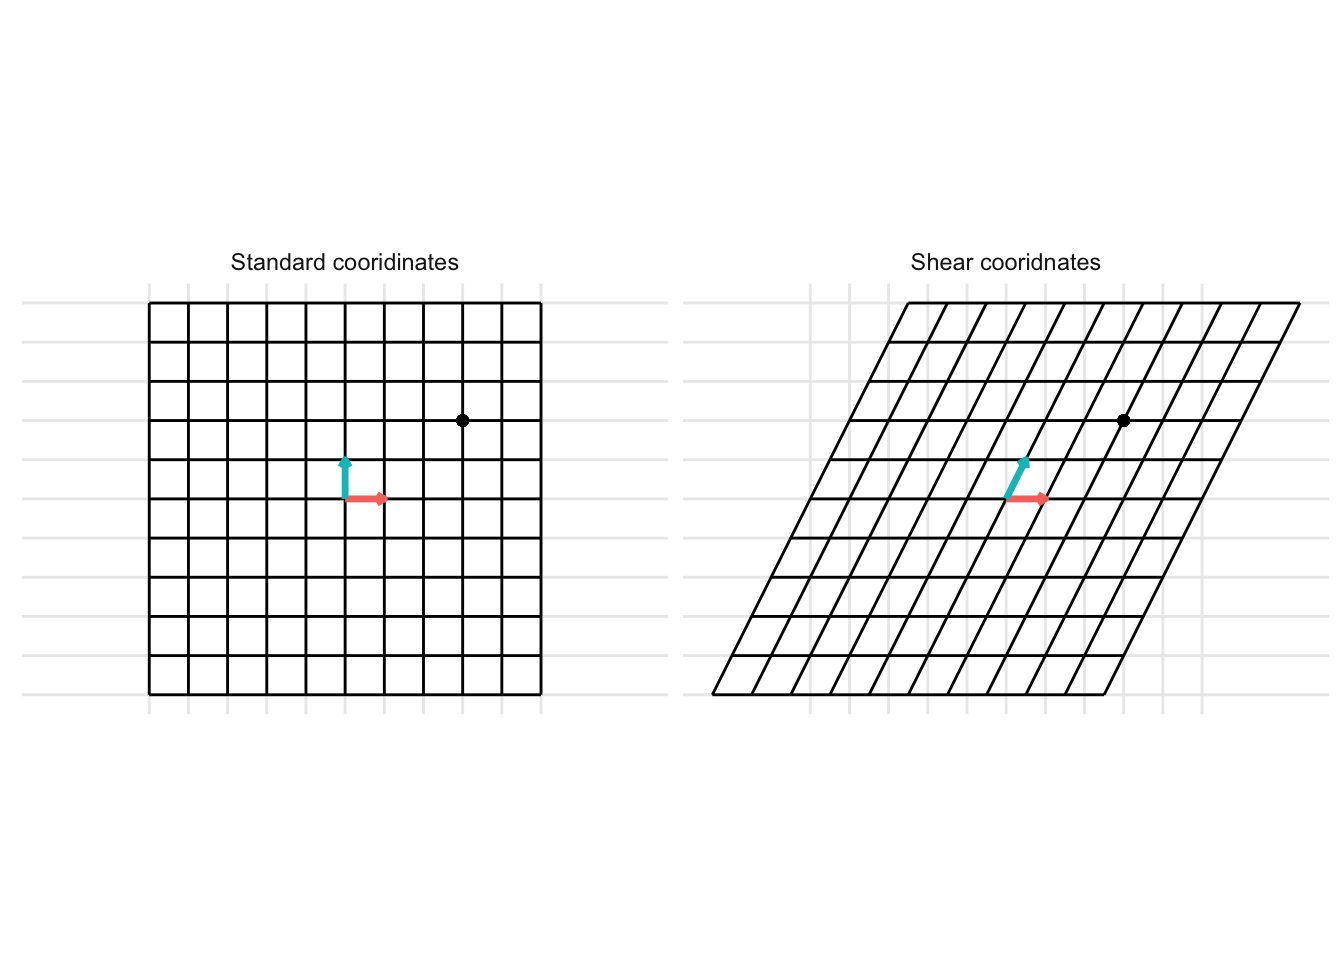
\includegraphics{multivariable-math_files/figure-latex/unnamed-chunk-170-1.pdf}

\hypertarget{coordinates-in-mathcalrn}{%
\section{\texorpdfstring{Coordinates in \(\mathcal{R}^n\)}{Coordinates in \textbackslash mathcal\{R\}\^{}n}}\label{coordinates-in-mathcalrn}}

Let \(\mathbf{x}\) be defined with the standard coordinates. Let \(\mathcal{B} = \{ \mathbf{b}_1, \ldots, \mathbf{b}_n \}\) be a basis in \(\mathcal{R}^n\). Define \(\mathbf{B} = \begin{pmatrix} \mathbf{b}_1 & \cdots & \mathbf{b}_n \end{pmatrix}\) as the matrix with columns the vectors of the basis. Then, the coordinates \(\left[\mathbf{x}\right]_B = \begin{pmatrix} [x_1]_B \\ \vdots \\ [x_n]_B \end{pmatrix}\) of \(\mathbf{x}\)

with respect to the basis \(\mathcal{B}\) can be found by solving the matrix equation

\[
\begin{aligned}
\mathbf{B} \left[\mathbf{x}\right]_B = \mathbf{x}
\end{aligned}
\]
The matrix \(\mathbf{B}\) is called the \textbf{change-of-coordinates matrix} from \(\mathcal{B}\) to the standard basis in \(\mathcal{R}^n\). The solution set (the coefficients) \(\left[\mathbf{x}\right]_B\) can be found using row operations or by using the fact that because the columns of \(\mathbf{B}\) spans \(\mathcal{R}^n\) the matrix \(\mathbf{B}\) is invertible. Then, the coordinates of \(\mathbf{x}\) with respect to the basis \(\mathcal{B}\) is
\[
\begin{aligned}
\left[\mathbf{x}\right]_B = \mathbf{B}^{-1} \mathbf{x}
\end{aligned}
\]

\begin{theorem}
Let \(\mathcal{B} = \{ \mathbf{b}_1, \ldots, \mathbf{b}_n\}\) be a basis for the vector space \(\mathcal{V}\). Then, the coordinate mapping \(\mathbf{x} \rightarrow \mathbf{B}^{-1} \mathbf{x}\) is a one-to-one and onto transformation from \(\mathcal{V}\) to \(\mathcal{R}^n\)
\end{theorem}

\begin{proof}

First we want to show that multiplication by \(\mathbf{B}^{-1}\) defines a linear transformation. First, take two vectors
\[
\begin{aligned}
\mathbf{u} &  = c_1 \mathbf{b}_1 + \ldots + c_n \mathbf{b}_n
\end{aligned}
\]
and
\[
\begin{aligned}
\mathbf{v} = d_1 \mathbf{b}_1 + \ldots + d_n \mathbf{b}_n
\end{aligned}
\]

\begin{itemize}
\tightlist
\item
  First, we show the mapping preserves vector addition
\end{itemize}

\[
\begin{aligned}
\mathbf{u} + \mathbf{v} \rightarrow \mathbf{B}^{-1} (\mathbf{u} + \mathbf{v}) =  \mathbf{B}^{-1} \mathbf{u} + \mathbf{B}^{-1} \mathbf{v}
\end{aligned}
\]
which preserves vector addition

\begin{itemize}
\tightlist
\item
  Next, we show the mapping preserves scalar multiplication. Given scalar \(a\),
\end{itemize}

\[
\begin{aligned}
a\mathbf{u} \rightarrow \mathbf{B}^{-1} (a \mathbf{u}) =  a \mathbf{B}^{-1} \mathbf{u}
\end{aligned}
\]
which preserves scalar multiplication.

\begin{itemize}
\tightlist
\item
  Therefore, this is a linear transformation. one-to-one and onto come from fact that \(\mathbf{B}\) is and \(n \times n\) matrix with \(n\) pivot columns (\(n\) linearly independent vectors because it is a basis for \(\mathcal{R}^n\))
\end{itemize}

\end{proof}

\begin{example}
in class--Give basis in \(\mathcal{R}^4\), find coefficients with respect to this basis for the vector \(\mathbf{x}\)
\end{example}

\hypertarget{dimension-of-a-vector-space}{%
\section{Dimension of a vector space}\label{dimension-of-a-vector-space}}

In some sense, we already know about the dimension of a vector space through the concept of a span. The span of a set of vectors defines the dimension of the vector space.

\begin{theorem}
In a vector space \(\mathcal{V}\) with basis \(\mathcal{B} = \{ \mathbf{b}_1, \ldots, \mathbf{b}_n\}\), any set in \(\mathcal{V}\) containing more than \(n\) vectors must be linearly dependent.
\end{theorem}

\begin{proof}
Let \(\{\mathbf{u}_1, \ldots, \mathbf{u}_p \}\) be a set of vectors in \(\mathcal{V}\) with \(p > n\). The coordinate vectors \(\{\mathbf{B} \mathbf{u}_1, \ldots, \mathbf{B} \mathbf{u}_p\}\) form a linearly dependent set in \(\mathcal{R}^n\) because there are more vectors (\(p\)) than entries (\(n\)) in each vector. Thus, there exist scalars \(c_1, \ldots, c_p\), some nonzero, such that
\[
\begin{aligned}
c_1 \mathbf{B} \mathbf{u}_1 + \ldots + c_p \mathbf{B} \mathbf{u}_p = \mathbf{0}.
\end{aligned}
\]
which by linearity implies
\[
\begin{aligned}
\mathbf{B} (c_1 \mathbf{u}_1 + \ldots + c_p \mathbf{u}_p) = \mathbf{0} 
\end{aligned}
\]
\end{proof}

Because the matrix \(\mathbf{B}\) is a \(n \times n\) matrix with n linearly independent columns, the only way the equation above can equal \(\mathbf{0}\) is if the vector \(c_1 \mathbf{u}_1 + \ldots + c_p \mathbf{u}_p = \mathbf{0}\) (by the invertible matrix theorem). Therefore, the set of vectors \(\{\mathbf{u}_1, \ldots, \mathbf{u}_p \}\) is linearly dependent because there are coefficients that allow the vectors to sum to \(\mathbf{0}\). Thus, we know that for a vector space \(\mathcal{V}\) that has a basis \({\mathcal{B} = \{ \mathbf{b}_1, \ldots, \mathbf{b}_n \}}\) that consists on \(n\) vectors, then every linearly independent set of vectors in \(\mathcal{V}\) contains at most \(n\) vectors.

\begin{theorem}
If a vector space \({\mathcal{V}}\) has a basis with \(n\) vectors, then every other basis of \({\mathcal{V}}\) must also contain exactly \(n\) vectors.
\end{theorem}

\begin{proof}
Let \(\mathcal{B}_1\) be a basis of \({\mathcal{V}}\) containing \(n\) vectors and let \(\mathcal{B}_2\) be any other basis of \({\mathcal{V}}\). Because \(\mathcal{B}_1\) and \(\mathcal{B}_2\) are both bases, they both contain sets of linearly independent vectors. As such, the previous theorem states that each of these bases contain at most \(n\) vectors (otherwise the sets wouldn't be linearly independent). Because \(\mathcal{B}_2\) is a basis and the basis \(\mathcal{B}_1\) contains \(n\) vectors, \(\mathcal{B}_2\) must contain at least \(n\) vectors. These results combined are only satisfied when \(\mathcal{B}_2\) contains \(n\) vectors.
\end{proof}

Like the span defined by the columns of a matrix \(\mathbf{A}\), there is an abstract concept called dimension which measures the ``size'' of a vector space.

\begin{definition}
If \({\mathcal{V}}\) is spanned by a finite set of vectors, then \({\mathcal{V}}\) is said to be finite dimensional. If \({\mathcal{V}}\) is not spanned by a finite set of vectors, \({\mathcal{V}}\) is said to be infinite dimensional. The smallest set of vectors that spans \({\mathcal{V}}\) is a basis for \({\mathcal{V}}\) and the number of vectors in this basis is called the \textbf{dimension} of \({\mathcal{V}}\) and written as dim(\({\mathcal{V}}\)). If \({\mathcal{V}}= \{\mathbf{0}\}\), then dim(\({\mathcal{V}}\)) is said to be 0.
\end{definition}

\begin{example}

in class - span of 2 or 3 linearly independent vectors

\begin{itemize}
\tightlist
\item
  span, dim, and geometry
\end{itemize}

\end{example}

\begin{example}

in class - span of 2 or 3 linearly dependent vectors

\begin{itemize}
\tightlist
\item
  span, dim, and geometry
\end{itemize}

\end{example}

\hypertarget{subspaces-of-finite-dimension}{%
\section{Subspaces of finite dimension}\label{subspaces-of-finite-dimension}}

\begin{theorem}
Let \(\mathcal{H}\) be a subspace of a finite-dimensional vector space \({\mathcal{V}}\). Then, any linearly independent set in \(\mathcal{H}\) can be expanded, if necessary to form a basis for \(\mathcal{H}\). As \(\mathcal{H}\) is a subspace of the finite-dimensional vector space \({\mathcal{V}}\), \(\mathcal{H}\) is a finite-dimensional vector space with
\[
\begin{aligned}
\mbox{dim}(\mathcal{H}) \leq \mbox{dim}(\mathcal{V})
\end{aligned}
\]
\end{theorem}

For a vector space of known dimension \(p\), finding a basis can be simplified by finding a linearly independent set of size \(p\).

\begin{theorem}[The Basis Theorem]
Let \(\mathcal{V}\) be a \(p\) dimensional vector space with \(p \geq 1\). Any linearly independent subset of \(p\) vectors is a basis for \(\mathcal{V}\). Equivalently, any set of \(p\) vectors that span \({\mathcal{V}}\) is automatically a basis for \(\mathcal{V}\).
\end{theorem}

\hypertarget{dimensions-of-nullmathbfa-and-colmathbfa}{%
\section{\texorpdfstring{Dimensions of null(\(\mathbf{A}\)) and col(\(\mathbf{A}\))}{Dimensions of null(\textbackslash mathbf\{A\}) and col(\textbackslash mathbf\{A\})}}\label{dimensions-of-nullmathbfa-and-colmathbfa}}

The dimension of null(\(\mathbf{A}\)) are the number of free variables in \(\mathbf{A}\mathbf{x} = \mathbf{0}\) and the dimension of col(\(\mathbf{A}\)) is the number of pivot columns of \(\mathbf{A}\).

\hypertarget{rank-1}{%
\chapter{Rank}\label{rank-1}}

\begin{Shaded}
\begin{Highlighting}[]
\KeywordTok{library}\NormalTok{(tidyverse)}
\KeywordTok{library}\NormalTok{(dasc2594)}
\end{Highlighting}
\end{Shaded}

\begin{definition}
Given an \(m \times n\) matrix \(\mathbf{A}\), the row space, row(\(\mathbf{A}\)) is the set of linearly independent rows of \(\mathbf{A}\). Thus, the row space is the span of the rows of \(\mathbf{A}\).
\end{definition}

Note: the row space of \(\mathbf{A}\) is the column space of the transposed matrix \(\mathcal{A}'\).
\[
\begin{aligned}
row(\mathbf{A}) = col(\mathbf{A}')
\end{aligned}
\]

\begin{example}
in class
\end{example}

\begin{example}
Find basis for row space, column space, and null space of \(\mathbf{A}\)
\end{example}

\hypertarget{rank-2}{%
\section{Rank}\label{rank-2}}

\begin{definition}
The rank of a matrix \(\mathbf{A}\), rank(\(\mathbf{A}\)) is the dimension of the column space col(\(\mathbf{A}\))
\end{definition}

\begin{theorem}[The Rank Theorem]
Let \(\mathbf{A}\) be an \(m \times n\) matrix. Then the dimension of are equal. The rank of \(\mathbf{A}\) equals the number of pivot columns of \(\mathbf{A}\) and
\[
\begin{aligned}
rank (\mathbf{A}) + dim(null(\mathbf{A})) = n
\end{aligned}
\]
\end{theorem}

\begin{proof}
The rank(\(\mathbf{A}\)) is the number of pivot columns and dim(null(\(\mathbf{A}\))) is the number of non-pivot columns. The number of pivot columns (rank(\(\mathbf{A}\))) + the number of non-pivot columns (dim(null(\(\mathbf{A}\)))) are the number of columns.
\end{proof}

\begin{example}
in class

\(\mathbf{A}\) is an \(m \times n\) matrix with dim(null(\(\mathbf{A}\))) = p.~What is rank(\(\mathbf{A}\))
\end{example}

\begin{example}
\(\mathbf{A}\) is a 6x9 matrix. Is it possible for null(\(\mathbf{A}\)) = 2?
\end{example}

\begin{theorem}[Invertible Matrix Theorm + Rank]
This is an extension of the prior statement of the invertible matrix theorem \ref{thm:invertible-matrix}
Let \(\mathbf{A}\) be an \(n \times n\) matrix. Then the following statements are equivalent (i.e., they are all either simultaneously true or false).

13) The columns of \(\mathbf{A}\) form a basis of \(\mathcal{R}^n\)

14) col(\(\mathbf{A}\)) = \(\mathcal{R}^n\)

15) dim(col(\(\mathbf{A}\))) = \(n\)

16) rank(\(\mathbf{A}\)) = \(n\)

17) null(\(\mathbf{A}\)) = \(\{\mathbf{0}\}\)

18) dim(null(\(\mathbf{A}\))) = 0
\end{theorem}

\hypertarget{change-of-basis}{%
\chapter{Change of basis}\label{change-of-basis}}

\begin{itemize}
\tightlist
\item
  \href{https://www.3blue1brown.com/lessons/change-of-basis}{3 Blue 1 Brown -- Change of basis}
\end{itemize}

\begin{Shaded}
\begin{Highlighting}[]
\KeywordTok{library}\NormalTok{(tidyverse)}
\KeywordTok{library}\NormalTok{(dasc2594)}
\end{Highlighting}
\end{Shaded}

Consider two bases \(\mathcal{B} = \{ \mathbf{b}_1, \ldots, \mathbf{b}_n \}\) and \(\mathcal{C} = \{ \mathbf{c}_1, \ldots, \mathbf{c}_n \}\) for a vector space \(\mathcal{V}\). If we have a vector \(\left[\mathbf{x}\right]_B\) with coordinates in \(\mathcal{B}\), what are the coordinates of \(\left[\mathbf{x}\right]_C\) with respect to \(\mathcal{C}\)?

\begin{itemize}
\tightlist
\item
  Recall: we know how to change from the standard coordinates to the basis \(\mathcal{B}\). If \(\mathbf{x}\) is a vector in the standard coordinates and \(\mathbf{B} = \begin{pmatrix} \mathbf{b}_1 & \ldots & \mathbf{b}_n \end{pmatrix}\) is a matrix with columns given by the basis \(\mathbf{B}\), the coordinates of \(\left[\mathbf{x}\right]_B\) of the vector \(\mathbf{x}\) with respect to the basis \(\mathcal{B}\) are
  \[
  \begin{aligned}
  \left[\mathbf{x}\right]_B = \mathbf{B}^{-1} \mathbf{x}
  \end{aligned}
  \]
  and, as a consequence, given a vector \(\left[\mathbf{x}\right]_B\) with coordinates with respect to the basis \(\mathcal{B}\), the vector of coefficients \(\mathbf{x}\) with standard coordinates is given by
  \[
  \begin{aligned}
  \mathbf{x} = \mathbf{B} \left[\mathbf{x}\right]_B.
  \end{aligned}
  \]
\end{itemize}

Notice that change of coordinates is a linear transformation from \(\mathcal{B}\) to \(\mathcal{C}\) with transformation matrix \(\mathbf{A}\). Despite the more complex notation, this is just another linear transformation {[}\href{https://www.youtube.com/watch?v=VGhij2qmOs4}{link}{]}.

:::\{.example\}
Show the change of basis from the basis \(\mathcal{B} = \left\{ \begin{pmatrix} \frac{1}{2} \\ 1 \end{pmatrix}, \begin{pmatrix} -1 \\ 0 \end{pmatrix}\right\}\) to the basis \(\mathcal{C} = \left\{ \begin{pmatrix} 0 \\ \frac{1}{2} \end{pmatrix}, \begin{pmatrix} 1 \\ -\frac{1}{2} \end{pmatrix}\right\}\). To do this, represent the columns that make up the basis \(\mathcal{B}\) as the matrix \(\mathbf{B} = \begin{pmatrix} \frac{1}{2} & -1 \\ 1 & 0 \end{pmatrix}\) and represent the columns that make up the basis \(\mathcal{C}\) as the matrix \(\mathbf{C} = \begin{pmatrix} 0 & \frac{1}{2} \\ 1 & -\frac{1}{2} \end{pmatrix}\). Then, the change of basis can be represented as

\begin{Shaded}
\begin{Highlighting}[]
\NormalTok{B <-}\StringTok{ }\KeywordTok{matrix}\NormalTok{(}\KeywordTok{c}\NormalTok{(}\DecValTok{1}\OperatorTok{/}\DecValTok{2}\NormalTok{, }\DecValTok{1}\NormalTok{, }\DecValTok{-1}\NormalTok{, }\DecValTok{0}\NormalTok{), }\DecValTok{2}\NormalTok{, }\DecValTok{2}\NormalTok{)}
\NormalTok{C <-}\StringTok{ }\KeywordTok{matrix}\NormalTok{(}\KeywordTok{c}\NormalTok{(}\DecValTok{0}\NormalTok{, }\DecValTok{1}\OperatorTok{/}\DecValTok{2}\NormalTok{, }\DecValTok{1}\NormalTok{, }\DecValTok{-1}\OperatorTok{/}\DecValTok{2}\NormalTok{), }\DecValTok{2}\NormalTok{, }\DecValTok{2}\NormalTok{)}

\NormalTok{p <-}\StringTok{ }\KeywordTok{plot_change_basis}\NormalTok{(B, C)}
\end{Highlighting}
\end{Shaded}

which can be represented with the static images

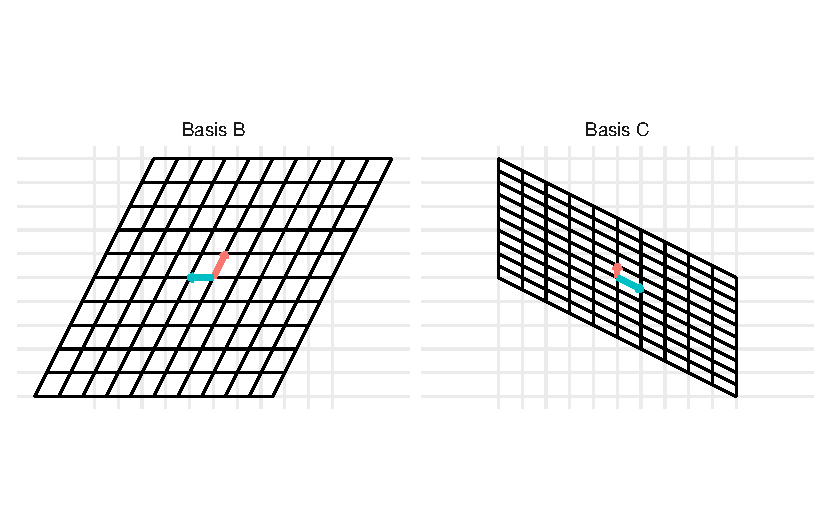
\includegraphics{multivariable-math_files/figure-latex/change-basis-static-1.pdf}

The change of basis represents a linear transformation. When previously discussing linear transformations in Chapter \ref{linear-transformations}, we considered a linear transformation from the standard basis \(\mathcal{I}\) defined by the basis vectors \(\left\{ \begin{pmatrix} 1 \\ 0 \end{pmatrix}, \begin{pmatrix} 0 \\ 1 \end{pmatrix} \right\}\) with the vectors represented as the columns of the identity matrix \(\mathbf{I}\). We can consider a change of basis as two consecutive linear transformations. First, a linear transformation from the basis \(\mathcal{B}\) to the standard basis \(\mathcal{I}\) and then a linear transformation from the standard basis \(\mathcal{I}\) to the basis \(\mathcal{C}\). This can be represented using the following example code:

\begin{Shaded}
\begin{Highlighting}[]
\NormalTok{p <-}\StringTok{ }\KeywordTok{plot_change_basis}\NormalTok{(B, C, }\DataTypeTok{plot_standard_basis =} \OtherTok{TRUE}\NormalTok{)}
\end{Highlighting}
\end{Shaded}

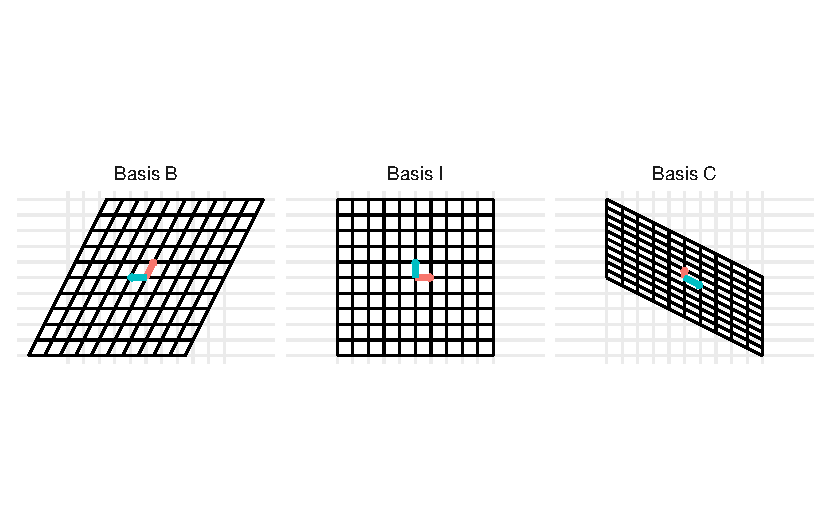
\includegraphics{multivariable-math_files/figure-latex/change-basis-I-static-1.pdf}

\hypertarget{changing-coordinates-between-different-bases}{%
\section{Changing coordinates between different bases}\label{changing-coordinates-between-different-bases}}

Now, we can combine these ideas. Given a vector \(\left[\mathbf{x}\right]_B\) written with coordinates with respect to the basis \(\mathcal{B}\), we can find the coordinates of \(\left[\mathbf{x}\right]_C\) with respect to the basis \(\mathcal{C}\). First, we find the coordinates of the vector \(\mathbf{x}\) with respect to the standard basis then find the coordinates of \(\left[\mathbf{x}\right]_C\) with respect to the basis \(\mathcal{C}\). Let \(\mathbf{B} = \begin{pmatrix} \mathbf{b}_1 & \ldots & \mathbf{b}_n \end{pmatrix}\) and \(\mathbf{C} = \begin{pmatrix} \mathbf{c}_1 & \ldots & \mathbf{c}_n \end{pmatrix}\), then given a vector \(\left[\mathbf{x}\right]_B\) with coordinates with respect to the basis \(\mathcal{B}\), the coordinates \(\left[\mathbf{x}\right]_C\) of this vector with respect to the basis \(\mathcal{C}\) is
\[
\begin{aligned}
\left[\mathbf{x}\right]_C = \mathbf{C}^{-1} \mathbf{B} \left[\mathbf{x}\right]_B.
\end{aligned}
\]

\textbf{Draw diagram}

\begin{example}

Working with the same bases \(\mathcal{B} = \left\{ \begin{pmatrix} \frac{1}{2} \\ 1 \end{pmatrix}, \begin{pmatrix} -1 \\ 0 \end{pmatrix}\right\}\) and \(\mathcal{C} = \left\{ \begin{pmatrix} 0 \\ \frac{1}{2} \end{pmatrix}, \begin{pmatrix} 1 \\ -\frac{1}{2} \end{pmatrix}\right\}\) from the previous example, Let \(\left[\mathbf{x}\right]_B = \begin{pmatrix} -3/2 \\ 1/2 \end{pmatrix}\) be the coordinates of the vector \(\mathbf{x}\) with respect to the basis \(\mathcal{B} = \left\{ \begin{pmatrix} 1/2 \\ 1 \end{pmatrix}, \begin{pmatrix} -1 \\ 0 \end{pmatrix}\right\}\). Find

\begin{enumerate}
\def\labelenumi{\arabic{enumi})}
\tightlist
\item
  the coordinates of \(\mathbf{x}\) with respect to the standard basis and
\item
  the coordinates of \(\mathbf{x}\) with respect to the basis \(\mathcal{C}\).
\end{enumerate}

\end{example}

\begin{solution}

Here we solve the two questions from the example above.

\begin{enumerate}
\def\labelenumi{\arabic{enumi})}
\tightlist
\item
  Recall that the coordinates \(\left[\mathbf{x}\right]_B\) of \(\mathbf{x}\) with respect to the basis \(\mathcal{B}\) mean that the vector \(\mathbf{x}\) can be written as a linear combination of the basis vectors \(\mathbf{b}_1\) and \(\mathbf{b}_2\) with coefficients given by the elements in \(\left[\mathbf{x}\right]_B = \begin{pmatrix} \left[x_1\right]_B \\ \left[x_2\right]_B \end{pmatrix}\). This results in the equation
\end{enumerate}

\[
\begin{aligned}
\mathbf{x} & = \left[x_1\right]_B \mathbf{b}_1 + \left[x_2\right]_B \mathbf{b}_2
\end{aligned}
\]
Plugging the values from the example gives
\[
\begin{aligned}
\mathbf{x} & = \left[x_1\right]_B \mathbf{b}_1 + \left[x_2\right]_B \mathbf{b}_2 \\
& = -1.5 \begin{pmatrix} 1/2 \\ 1 \end{pmatrix} + 0.5 \begin{pmatrix} -1 \\ 0 \end{pmatrix} \\
& = \begin{pmatrix} -3/4 \\ -3/2 \end{pmatrix} + \begin{pmatrix} -1/2 \\ 0 \end{pmatrix} \\
& = \begin{pmatrix} -5/4 \\ -3/2 \end{pmatrix}
\end{aligned}
\]
2) Now, recall the coordinates \(\left[\mathbf{x}\right]_C\) of \(\mathbf{x}\) with respect to the basis \(\mathcal{C}\) mean that the vector \(\mathbf{x}\) can be written as a linear combination of the basis vectors \(\mathbf{c}_1\) and \(\mathbf{c}_2\) with coefficients given by the elements in \(\left[\mathbf{x}\right]_C = \begin{pmatrix} \left[x_1\right]_C \\ \left[x_2\right]_C \end{pmatrix}\). This results in the equation

\[
\begin{aligned}
\mathbf{x} & = \left[x_1\right]_C \mathbf{c}_1 + \left[x_2\right]_C \mathbf{c}_2
\end{aligned}
\]
However, unlike part (1), we do not know the coefficients \(\left[\mathbf{x}\right]\) but need to solve for them. Rewriting the above equation in the form of \(\mathbf{A}\mathbf{x} = \mathbf{b}\) gives
\[
\begin{aligned}
\mathbf{C} \left[ \mathbf{x} \right]_C & = \mathbf{x}
\end{aligned}
\]
Because the matrix of basis vectors \(\mathbf{C}\) is an invertible matrix (a basis is a linearly independent spanning set), the coefficients \(\left[\mathbf{x}\right]_C\) can be solved using the equation
\[
\begin{aligned}
\mathbf{C} \left[ \mathbf{x} \right]_C & = \mathbf{x} \\
\mathbf{C}^{-1} \mathbf{C}\left[ \mathbf{x} \right]_C & = \mathbf{C}^{-1}\mathbf{x} \\
\left[ \mathbf{x} \right]_C & = \mathbf{C}^{-1} \mathbf{x} 
\end{aligned}
\]
The matrix inverse \(\mathbf{C}^{-1}\) can be found using theorem \ref{thm:matrix-2by2} to get \(\mathbf{C}^{-1} = \begin{pmatrix} 1 & 2 \\ 1 & 0 \end{pmatrix}\). Then, plugging in the values from the example gives

\[
\begin{aligned}
\left[ \mathbf{x} \right]_C & = \mathbf{C}^{-1} \mathbf{x} \\
& = \begin{pmatrix} 1 & 2 \\ 1 & 0 \end{pmatrix} \begin{pmatrix} -5/4 \\ -3/2 \end{pmatrix} \\
& = \begin{pmatrix} -17/4 \\ -5/4 \end{pmatrix}
\end{aligned}
\]
Another way to change coordinates is to change directly from basis \(\mathcal{B}\) to \(\mathcal{C}\) without going through the intermediate transformation to the standard coordinates. Combining the results from (1) and (2) gives
\[
\begin{aligned}
\left[ \mathbf{x} \right]_C & = \mathbf{C}^{-1} \mathbf{x} \\
& = \mathbf{C}^{-1} \mathbf{B} \left[\mathbf{x}\right]_B
\end{aligned}
\]
so that one can change coordinates from the basis \(\mathcal{B}\) to the basis \(\mathcal{C}\) using the linear transformation defined by the matrix multiplication \(\mathbf{C}^{-1} \mathbf{B}\).

In \texttt{R}, first define the basis matrices \texttt{B} and \texttt{C} and the coordinates \texttt{x\_b} of the vector \(\mathbf{x}\) with respect to the basis \(\mathcal{B}\).

\begin{Shaded}
\begin{Highlighting}[]
\NormalTok{B <-}\StringTok{ }\KeywordTok{matrix}\NormalTok{(}\KeywordTok{c}\NormalTok{(}\DecValTok{1}\OperatorTok{/}\DecValTok{2}\NormalTok{, }\DecValTok{1}\NormalTok{, }\DecValTok{-1}\NormalTok{, }\DecValTok{0}\NormalTok{), }\DecValTok{2}\NormalTok{, }\DecValTok{2}\NormalTok{)}
\NormalTok{C <-}\StringTok{ }\KeywordTok{matrix}\NormalTok{(}\KeywordTok{c}\NormalTok{(}\DecValTok{0}\NormalTok{, }\DecValTok{1}\OperatorTok{/}\DecValTok{2}\NormalTok{, }\DecValTok{1}\NormalTok{, }\DecValTok{-1}\OperatorTok{/}\DecValTok{2}\NormalTok{), }\DecValTok{2}\NormalTok{, }\DecValTok{2}\NormalTok{)}
\NormalTok{x_b <-}\StringTok{ }\KeywordTok{c}\NormalTok{(}\OperatorTok{-}\DecValTok{3}\OperatorTok{/}\DecValTok{2}\NormalTok{, }\DecValTok{1}\OperatorTok{/}\DecValTok{2}\NormalTok{)}
\end{Highlighting}
\end{Shaded}

1) The coordinates \texttt{x} with respect to the standard basis is

\begin{Shaded}
\begin{Highlighting}[]
\NormalTok{x <-}\StringTok{ }\NormalTok{B }\OperatorTok\StringTok{ }\NormalTok{x_b}
\NormalTok{x}
\end{Highlighting}
\end{Shaded}

\begin{verbatim}
##       [,1]
## [1,] -1.25
## [2,] -1.50
\end{verbatim}

2) The coordinates \texttt{x\_c} with respect to the basis \(\mathcal{C}\) can be found by calculating the matrix inverse \texttt{C\_inv} and then using the matrix inverse to calculate the coordinates with respect to the basis \(\mathcal{C}\) as

\begin{Shaded}
\begin{Highlighting}[]
\NormalTok{C_inv <-}\StringTok{ }\KeywordTok{solve}\NormalTok{(C)}
\NormalTok{x_c <-}\StringTok{ }\NormalTok{C_inv }\OperatorTok\StringTok{ }\NormalTok{x}
\NormalTok{x_c}
\end{Highlighting}
\end{Shaded}

\begin{verbatim}
##       [,1]
## [1,] -4.25
## [2,] -1.25
\end{verbatim}

Done as a single transformation, the linear transformation is defined as

\begin{Shaded}
\begin{Highlighting}[]
\NormalTok{B }\OperatorTok\StringTok{ }\NormalTok{C_inv}
\end{Highlighting}
\end{Shaded}

\begin{verbatim}
##      [,1] [,2]
## [1,] -0.5    1
## [2,]  1.0    2
\end{verbatim}

which gives the coordinates

\begin{Shaded}
\begin{Highlighting}[]
\NormalTok{B }\OperatorTok\StringTok{ }\NormalTok{C_inv }\OperatorTok\StringTok{ }\NormalTok{x_b}
\end{Highlighting}
\end{Shaded}

\begin{verbatim}
##       [,1]
## [1,]  1.25
## [2,] -0.50
\end{verbatim}

\end{solution}

\begin{example}
3-d change of basis
\end{example}

\hypertarget{eigenvectors-and-eigenvalues}{%
\chapter{Eigenvectors and Eigenvalues}\label{eigenvectors-and-eigenvalues}}

\begin{itemize}
\tightlist
\item
  \href{https://www.3blue1brown.com/lessons/eigenvalues}{3 Blue 1 Brown -- Eigenvalues}
\end{itemize}

\begin{Shaded}
\begin{Highlighting}[]
\KeywordTok{library}\NormalTok{(tidyverse)}
\KeywordTok{library}\NormalTok{(dasc2594)}
\KeywordTok{set.seed}\NormalTok{(}\DecValTok{2021}\NormalTok{)}
\end{Highlighting}
\end{Shaded}

We have just learned about change of basis in an abstract sense. Now, we will learn about a special change of basis that is ``data-driven'' called an eigenvector. Eigenvectors and the corresponding eigenvalues are a vital tool in data science for data compression and modeling.

\begin{definition}
An \textbf{eigenvector} of an \(n \times n\) matrix \(\mathbf{A}\) is a nonzero vector \(\mathbf{x}\) such that the matrix equation
\[
\begin{aligned}
\mathbf{A} \mathbf{x} = \lambda \mathbf{x}
\end{aligned}
\]
for some scalar \(\lambda\). If there exists some \(\lambda \neq 0\) (a non-trivial solutions), then \(\lambda\) is called an \textbf{eigenvalue} of \(\mathbf{A}\) corresponding to the eigenvector \(\mathbf{x}\).
\end{definition}

\begin{example}
It is easy to check if a vector is an eigenvalue:

Let \(\mathbf{A} = \begin{pmatrix} 0 & 6 & 8 \\ 1/2 & 0 & 0 \\ 0 & 1/2 & 0 \end{pmatrix}\), \(\mathbf{u} = \begin{pmatrix} 16 \\ 4 \\ 1 \end{pmatrix}\), and \(\mathbf{v} = \begin{pmatrix} 2 \\ 2 \\ 2 \end{pmatrix}\). Determine if \(\mathbf{u}\) or \(\mathbf{v}\) are eigenvectors of \(\mathbf{A}\). If they are eigenvectors, what are the associated eigenvalues.
\end{example}

\begin{solution}

Here we demonstrate the eigenvector/eigenvalue relationship.

\begin{enumerate}
\def\labelenumi{\alph{enumi})}
\tightlist
\item
  If \(\mathbf{u}\) is an eigenvector of a matrix \(\mathbf{A}\), then there exists some constant \(\lambda\) such that \(\mathbf{A} \mathbf{u} = \lambda \mathbf{u}\). Checking this gives
  \[
  \begin{aligned}
  \mathbf{A} \mathbf{u} & = \begin{pmatrix} 0 & 6 & 8 \\ 1/2 & 0 & 0 \\ 0 & 1/2 & 0 \end{pmatrix} \begin{pmatrix} 16 \\ 4 \\ 1 \end{pmatrix} \\
  & = \begin{pmatrix} 32 \\ 8 \\ 2 \end{pmatrix} \\ 
  & = 2 \begin{pmatrix} 16 \\ 4 \\ 1 \end{pmatrix}
  \end{aligned}
  \]
  which shows that \(\mathbf{u}\) is an eigenvector of \(\mathbf{A}\) with associated eigenvalue \(\lambda = 2\). Now, we check if \(\mathbf{v}\) is an eigenvector of \(\mathbf{A}\)
  \[
  \begin{aligned}
  \mathbf{A} \mathbf{v} & = \begin{pmatrix} 0 & 6 & 8 \\ 1/2 & 0 & 0 \\ 0 & 1/2 & 0 \end{pmatrix} \begin{pmatrix} 2 \\ 2 \\ 2 \end{pmatrix} \\
  & = \begin{pmatrix} 28 \\ 1 \\ 1 \end{pmatrix} 
  \end{aligned}
  \]
  where there is no number \(\lambda\) such that \(\begin{pmatrix} 28 \\ 1 \\ 1 \end{pmatrix} = \lambda \begin{pmatrix} 2 \\ 2 \\ 2 \end{pmatrix}\). In \texttt{R}, this can be shown
\end{enumerate}

\begin{Shaded}
\begin{Highlighting}[]
\NormalTok{A <-}\StringTok{ }\KeywordTok{matrix}\NormalTok{(}\KeywordTok{c}\NormalTok{(}\DecValTok{0}\NormalTok{, }\DecValTok{1}\OperatorTok{/}\DecValTok{2}\NormalTok{, }\DecValTok{0}\NormalTok{, }\DecValTok{6}\NormalTok{, }\DecValTok{0}\NormalTok{, }\DecValTok{1}\OperatorTok{/}\DecValTok{2}\NormalTok{, }\DecValTok{8}\NormalTok{, }\DecValTok{0}\NormalTok{, }\DecValTok{0}\NormalTok{), }\DecValTok{3}\NormalTok{, }\DecValTok{3}\NormalTok{)}
\NormalTok{A}
\end{Highlighting}
\end{Shaded}

\begin{verbatim}
##      [,1] [,2] [,3]
## [1,]  0.0  6.0    8
## [2,]  0.5  0.0    0
## [3,]  0.0  0.5    0
\end{verbatim}

\begin{Shaded}
\begin{Highlighting}[]
\NormalTok{u <-}\StringTok{ }\KeywordTok{c}\NormalTok{(}\DecValTok{16}\NormalTok{, }\DecValTok{4}\NormalTok{, }\DecValTok{1}\NormalTok{)}
\NormalTok{v <-}\StringTok{ }\KeywordTok{c}\NormalTok{(}\DecValTok{2}\NormalTok{, }\DecValTok{2}\NormalTok{, }\DecValTok{2}\NormalTok{)      }
\CommentTok{# is u an eigenvector of A?}
\NormalTok{A }\OperatorTok\StringTok{ }\NormalTok{u}
\end{Highlighting}
\end{Shaded}

\begin{verbatim}
##      [,1]
## [1,]   32
## [2,]    8
## [3,]    2
\end{verbatim}

\begin{Shaded}
\begin{Highlighting}[]
\CommentTok{# yes, because A %*% u = 2 u}
\CommentTok{# 2 is the eigenvalue associated with u}

\CommentTok{# is v an eigenvector of A?}
\NormalTok{A }\OperatorTok\StringTok{ }\NormalTok{v}
\end{Highlighting}
\end{Shaded}

\begin{verbatim}
##      [,1]
## [1,]   28
## [2,]    1
## [3,]    1
\end{verbatim}

\begin{Shaded}
\begin{Highlighting}[]
\CommentTok{# not an eigenvectos because A %*% v is not equal to lambda * v for some lambda}
\end{Highlighting}
\end{Shaded}

\end{solution}

\begin{example}
It is easy to check if a vector is an eigenvalue:

Let \(\mathbf{A} = \begin{pmatrix} 2 & 1 \\ 0 & 1 \end{pmatrix}\), \(\mathbf{u} = \begin{pmatrix} - \frac{\sqrt{2}}{2} \\ \frac{\sqrt{2}}{2} \end{pmatrix}\), and \(\mathbf{v} = \begin{pmatrix} 1 \\ 1 \end{pmatrix}\). Determine if \(\mathbf{u}\) or \(\mathbf{v}\) are eigenvectors of \(\mathbf{A}\). If they are eigenvectors, what are the associated eigenvalues. Now, plot \(\mathbf{u}\), \(\mathbf{A} \mathbf{u}\), \(\mathbf{v}\), and \(\mathbf{A} \mathbf{v}\) to show this relationship geometrically.
\end{example}

\begin{solution}
First, we determine if the vectors \(\mathbf{u}\) and \(\mathbf{v}\) are eigenvectors of \(\mathbf{A}\).

If \(\mathbf{u}\) is an eigenvector of a matrix \(\mathbf{A}\), then there exists some constant \(\lambda\) such that \(\mathbf{A} \mathbf{u} = \lambda \mathbf{u}\). Checking this gives
\[
\begin{aligned}
\mathbf{A} \mathbf{u} & = \begin{pmatrix} 2 & 1 \\ 0 & 1 \end{pmatrix} \begin{pmatrix} - \frac{\sqrt{2}}{2} \\ \frac{\sqrt{2}}{2} \end{pmatrix} \\
& = \begin{pmatrix} - \frac{\sqrt{2}}{2} \\ \frac{\sqrt{2}}{2} \end{pmatrix} 
\end{aligned}
\]
which shows that \(\mathbf{u}\) is an eigenvector of \(\mathbf{A}\) with associated eigenvalue \(\lambda = 1\). Now, we check if \(\mathbf{v}\) is an eigenvector of \(\mathbf{A}\)
\[
\begin{aligned}
\mathbf{A} \mathbf{v} & = \begin{pmatrix} 2 & 1 \\ 0 & 1 \end{pmatrix} \begin{pmatrix} 1 \\ 1 \end{pmatrix} \\
& = \begin{pmatrix} 3 \\ 1 \end{pmatrix} 
\end{aligned}
\]
where there is no number \(\lambda\) such that \(\begin{pmatrix} 3 \\ 1 \end{pmatrix} = \lambda \begin{pmatrix} 1 \\ 1 \end{pmatrix}\). In \texttt{R}, this can be shown

\begin{Shaded}
\begin{Highlighting}[]
\NormalTok{A <-}\StringTok{ }\KeywordTok{matrix}\NormalTok{(}\KeywordTok{c}\NormalTok{(}\DecValTok{2}\NormalTok{, }\DecValTok{0}\NormalTok{, }\DecValTok{1}\NormalTok{, }\DecValTok{1}\NormalTok{), }\DecValTok{2}\NormalTok{, }\DecValTok{2}\NormalTok{)}
\NormalTok{u <-}\StringTok{ }\KeywordTok{c}\NormalTok{(}\OperatorTok{-}\KeywordTok{sqrt}\NormalTok{(}\DecValTok{2}\NormalTok{)}\OperatorTok{/}\DecValTok{2}\NormalTok{, }\KeywordTok{sqrt}\NormalTok{(}\DecValTok{2}\NormalTok{) }\OperatorTok{/}\StringTok{ }\DecValTok{2}\NormalTok{)}
\NormalTok{v <-}\StringTok{ }\KeywordTok{c}\NormalTok{(}\DecValTok{1}\NormalTok{, }\DecValTok{1}\NormalTok{)}

\CommentTok{# is u an eigenvector of A?}
\NormalTok{A }\OperatorTok\StringTok{ }\NormalTok{u}
\end{Highlighting}
\end{Shaded}

\begin{verbatim}
##            [,1]
## [1,] -0.7071068
## [2,]  0.7071068
\end{verbatim}

\begin{Shaded}
\begin{Highlighting}[]
\CommentTok{# yes, because A %*% u = u}
\CommentTok{# 1 is the eigenvalue associated with u}

\CommentTok{# is v an eigenvector of A?}
\NormalTok{A }\OperatorTok\StringTok{ }\NormalTok{v}
\end{Highlighting}
\end{Shaded}

\begin{verbatim}
##      [,1]
## [1,]    3
## [2,]    1
\end{verbatim}

\begin{Shaded}
\begin{Highlighting}[]
\CommentTok{# not an eigenvectos because A %*% v is not equal to lambda * v for some lambda}
\end{Highlighting}
\end{Shaded}

Now, we will plot the vectors \(\mathbf{u}\) and \(\mathbf{v}\) as well as the vectors transformed by the matrix \(\mathbf{A}\) (i.e., \(\mathbf{A} \mathbf{u}\) and \(\mathbf{A} \mathbf{v}\)). The code below plot the vector \(\mathbf{u}\) in dark blue and the transformed vector \(\mathbf{A} \mathbf{u}\) in light blue. The code also plots the vector \(\mathbf{v}\) in dark red and the transformed vector \(\mathbf{A} \mathbf{v}\) in light red.

\begin{Shaded}
\begin{Highlighting}[]
\KeywordTok{ggplot}\NormalTok{() }\OperatorTok{+}
\StringTok{    }\KeywordTok{geom_segment}\NormalTok{(}\KeywordTok{aes}\NormalTok{(}\DataTypeTok{x =} \DecValTok{0}\NormalTok{, }\DataTypeTok{xend =}\NormalTok{ u[}\DecValTok{1}\NormalTok{], }\DataTypeTok{y =} \DecValTok{0}\NormalTok{, }\DataTypeTok{yend =}\NormalTok{ u[}\DecValTok{2}\NormalTok{]), }\DataTypeTok{color =} \StringTok{"dark blue"}\NormalTok{) }\OperatorTok{+}
\StringTok{    }\KeywordTok{geom_segment}\NormalTok{(}\KeywordTok{aes}\NormalTok{(}\DataTypeTok{x =} \DecValTok{0}\NormalTok{, }\DataTypeTok{xend =}\NormalTok{ (A }\OperatorTok\StringTok{ }\NormalTok{u)[}\DecValTok{1}\NormalTok{], }\DataTypeTok{y =} \DecValTok{0}\NormalTok{, }\DataTypeTok{yend =}\NormalTok{ (A }\OperatorTok\StringTok{ }\NormalTok{u)[}\DecValTok{2}\NormalTok{]), }\DataTypeTok{color =} \StringTok{"light blue"}\NormalTok{, }\DataTypeTok{lty =} \DecValTok{2}\NormalTok{) }\OperatorTok{+}
\StringTok{    }\KeywordTok{geom_segment}\NormalTok{(}\KeywordTok{aes}\NormalTok{(}\DataTypeTok{x =} \DecValTok{0}\NormalTok{, }\DataTypeTok{xend =}\NormalTok{ v[}\DecValTok{1}\NormalTok{], }\DataTypeTok{y =} \DecValTok{0}\NormalTok{, }\DataTypeTok{yend =}\NormalTok{ v[}\DecValTok{2}\NormalTok{]), }\DataTypeTok{color =} \StringTok{"dark red"}\NormalTok{) }\OperatorTok{+}
\StringTok{    }\KeywordTok{geom_segment}\NormalTok{(}\KeywordTok{aes}\NormalTok{(}\DataTypeTok{x =} \DecValTok{0}\NormalTok{, }\DataTypeTok{xend =}\NormalTok{ (A }\OperatorTok\StringTok{ }\NormalTok{v)[}\DecValTok{1}\NormalTok{], }\DataTypeTok{y =} \DecValTok{0}\NormalTok{, }\DataTypeTok{yend =}\NormalTok{ (A }\OperatorTok\StringTok{ }\NormalTok{v)[}\DecValTok{2}\NormalTok{]), }\DataTypeTok{color =} \StringTok{"red"}\NormalTok{) }\OperatorTok{+}
\StringTok{    }\KeywordTok{coord_cartesian}\NormalTok{(}\DataTypeTok{xlim =} \KeywordTok{c}\NormalTok{(}\OperatorTok{-}\DecValTok{5}\NormalTok{, }\DecValTok{5}\NormalTok{), }\DataTypeTok{ylim =} \KeywordTok{c}\NormalTok{(}\OperatorTok{-}\DecValTok{5}\NormalTok{, }\DecValTok{5}\NormalTok{))}
\end{Highlighting}
\end{Shaded}

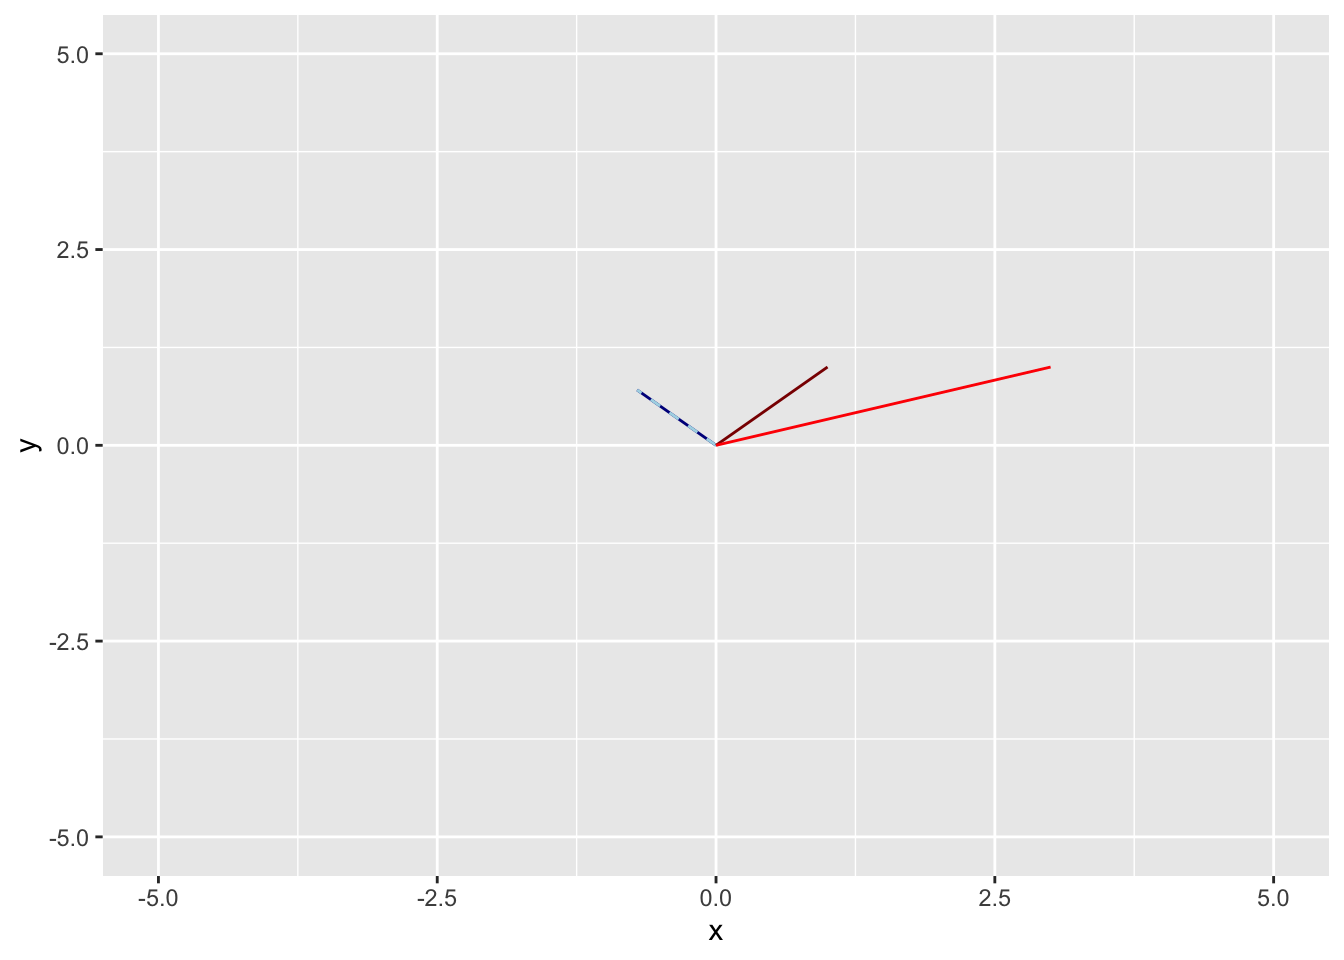
\includegraphics{multivariable-math_files/figure-latex/unnamed-chunk-184-1.pdf}
Notice that the multiplication of \(\mathbf{u}\) by \(\mathbf{A}\) gives a vector \(\mathbf{A} \mathbf{u}\) that points along the same line as \(\mathbf{u}\) because \(\mathbf{u}\) is an eigenvector of \(\mathbf{A}\). In comparison, the vector \(\mathbf{v}\) is not an eigenvector of \(\mathbf{A}\) and multiplication of \(\mathbf{v}\) by \(\mathbf{A}\) gives a vector \(\mathbf{A} \mathbf{v}\) that \emph{does not} point along the same line as the vector \(\mathbf{u}\).
\end{solution}

\begin{example}
Come up with another example and another plot that shows the similar result as the example above.
\end{example}

\begin{solution}
The solution (TBD)
\end{solution}

Thus, we end up with the understanding that nn eigenvector is a (nonzero) vector \(\mathbf{x}\) that gets mapped to a scalar multiple of itself \(\lambda \mathbf{x}\) by the matrix transformation defined by \(T: \mathbf{x} \rightarrow \mathbf{A}\mathbf{x} = \mathbf{x}\). As such, when \(\mathbf{x}\) is an eigenvector of \(\mathbf{A}\) we say that \(\mathbf{x}\) and \(\mathbf{A} \mathbf{x}\) are collinear with the origin (\(\mathbf{0}\)) and each other in the sense that these points lie on the same line that goes through the origin.

\textbf{Note:} The matrix \(\mathbf{A}\) must be an \(n \times n\) square matrix. A similar decomposition (called the singular value decomposition) can be used for rectangular matrices.

\begin{example}
Example: reflection
Draw images: \url{https://textbooks.math.gatech.edu/ila/eigenvectors.html}
\end{example}

\begin{theorem}[The distinct eigenvalues theorem]
\protect\hypertarget{thm:distinct-eigenvalues}{}\label{thm:distinct-eigenvalues}Let \(\mathbf{v}_1, \ldots, \mathbf{v}_n\) be eigenvectors of a matrix \(\mathbf{A}\) and suppose the corresponding eigenvalues are \(\lambda_1, \lambda_2, \ldots, \lambda_n\) are all distinct (different values). Then, the set of vectors \(\{\mathbf{v}_1, \ldots, \mathbf{v}_n\}\) is linearly independent.
\end{theorem}

\begin{proof}
Suppose the set \(\{\mathbf{v}_1, \ldots, \mathbf{v}_n\}\) is linearly dependent. Then, there is some \(j\) such that \(\mathbf{v}_j = \sum_{k = 1}^{j-1} x_k \mathbf{v}_k\). If we choose the first linearly dependent vector as \(j\), we know that the subset of vectors \(\{\mathbf{v}_1, \ldots, \mathbf{v}_{j-1}\}\) is linearly independent and
\[
\begin{aligned}
\mathbf{v}_j & = x_1 \mathbf{v}_1 + \cdots x_{j-1} + \mathbf{v}_{j-1}
\end{aligned}
\]
for some scalars \(x_1, \ldots, x_{j-1}\). Multiplying the equation above on the left by \(\mathbf{A}\) on both sides gives
\[
\begin{aligned}
\mathbf{A}\mathbf{v}_j & = \mathbf{A} (x_1 \mathbf{v}_1 + \cdots + x_{j-1} \mathbf{v}_{j-1}) \\
\lambda_j \mathbf{v}_j & = x_1 \mathbf{A} \mathbf{v}_1 + \cdots + x_{j-1} \mathbf{A} \mathbf{v}_{j-1} \\
& =  x_1 \lambda_1 \mathbf{v}_1 + \cdots x_{j-1} \lambda_{j-1} + \mathbf{v}_{j-1} \\
\end{aligned}
\]
Multiplying the first equation by \(\lambda_j\) and subtracting this from the second equation gives
\[
\begin{aligned}
\mathbf{0} = \lambda_j \mathbf{v}_j - \lambda_j \mathbf{v}_j 
& = x_1 (\lambda_1 - \lambda_j) \mathbf{v}_1 + \cdots x_{j-1} + (\lambda_{j-1} - \lambda_j) \mathbf{v}_{j-1} \\
\end{aligned}
\]
Because \(\lambda_k \neq \lambda_j\) for all \(k < j\), the equation above implies a linear dependence among the set of vectors \(\{\mathbf{v}_1, \ldots, \mathbf{v}_{j-1}\}\) which is a contradiction. Therefore, our assumption that there exists a linearly dependent vector \(\mathbf{v}_j\) is violated and all the \(\{\mathbf{v}_1, \ldots, \mathbf{v}_n\}\) are linearly independent.
\end{proof}

\hypertarget{eigenspaces}{%
\section{Eigenspaces}\label{eigenspaces}}

Given a square \(n \times n\) matrix \(\mathbf{A}\), we know how to check if a given vector \(\mathbf{x}\) is an eigenvector and then how to find the eigenvalue associated with that eigenvector. Next, we want to check if a given number is an eigenvalue of \(\mathbf{A}\) and to find all the eigenvectors corresponding to that eigenvalue.

Given a square \(n \times n\) matrix \(\mathbf{A}\) and a scalar \(\lambda\), the eigenvectors of \(\mathbf{A}\) associated with the scalar \(\lambda\) (if there are eigenvectors associated with \(\lambda\)) are the nonzero solutoins to the equation \(\mathbf{A} \mathbf{x} = \lambda \mathbf{x}\). This can be written as
\[
\begin{aligned}
\mathbf{A} \mathbf{x} & = \lambda \mathbf{x} \\
\mathbf{A} \mathbf{x} -\lambda \mathbf{x} & = \mathbf{0} \\
\mathbf{A} \mathbf{x} -\lambda \mathbf{I} \mathbf{x} & = \mathbf{0} \\
\left( \mathbf{A} -\lambda \mathbf{I} \right) \mathbf{x} & = \mathbf{0}. \\
\end{aligned}
\]
Therefore, the eigenvectors of \(\mathbf{A}\) associated with \(\lambda\), if there are any, are the nontrivial solutions of the homogeneous matrix equation \(\left( \mathbf{A} - \lambda \mathbf{I} \right) \mathbf{x} = \mathbf{0}\). In other words, the eigenvectors are the nonzero vectors in the null space null\(\left( \mathbf{A} -\lambda \mathbf{I} \right)\). If there is not a nontrivial solution (solution \(\mathbf{x} \neq \mathbf{0}\)), then \(\lambda\) is not an eigenvalue of \(\mathbf{A}\).

Hey, we know how to find solutions to homogeneous systems of equations! Thus, we know how to find the eigenvectors of \(\mathbf{A}\). All we have to do is solve the system of linear equations \(\left( \mathbf{A} -\lambda \mathbf{I} \right) \mathbf{x} = \mathbf{0}\) for a given \(\lambda\) (actually, for all \(\lambda\)s, which we can't do). If only there was some way to find eigenvalues \(\lambda\) (hint: there is and it is coming next chapter).

\begin{example}
Let \(\mathbf{A} = \begin{pmatrix} 3 & 6 & -8 \\ 0 & 0 & 6 \\ 0 & 0 & 2 \end{pmatrix}\). Then an eigenvector with eigenvector \(\lambda\) is a nontrival solution to
\[
\begin{aligned}
\left( \mathbf{A} - \lambda \mathbf{I} \right) \mathbf{x} & = \mathbf{0}
\end{aligned}
\]
which can be written as
\[
\begin{aligned}
\begin{pmatrix} 
3  - \lambda & 6 & -8 \\
0 & 0 - \lambda & 6 \\
0 & 0 & 2 - \lambda
\end{pmatrix} \begin{pmatrix} x_1 \\ x_2 \\ x_3 \end{pmatrix} & = \mathbf{0}
\end{aligned}
\]
which can be solved for a given \(\lambda\) using an augmented matrix form and row operations to reduce to reduced row echelon form.

Letting \(\lambda = 3\), we have
\[
\begin{aligned}
\begin{pmatrix} 
3  - 3 & 6 & -8 \\
0 & 0 - 3 & 6 \\
0 & 0 & 2 - 3
\end{pmatrix} \begin{pmatrix} x_1 \\ x_2 \\ x_3 \end{pmatrix} & = \mathbf{0}
\end{aligned}
\]
which can be written as the matrix equation
\[
\begin{aligned}
\begin{pmatrix} 0 & 6 & -8 \\ 0 & -3 & 6 \\ 0 & 0 & -1 \end{pmatrix} \begin{pmatrix} x_1 \\ x_2 \\ x_3 \end{pmatrix} & = \mathbf{0}
\end{aligned}
\]
Note that the columns of the matrix above are not linearly independent. Thus, we can solve a non-unique solution (the solution set is a line going through the origin) by finding the reduce row echelon form of an augmented matrix
\[
\begin{aligned}
\begin{pmatrix} 0 & 6 & -8 & 0 \\ 0 & -3 & 6 & 0 \\ 0 & 0 & -1 & 0 \end{pmatrix} & \stackrel{rref}{\huge \sim} \begin{pmatrix} 0 & 1 & 0 & 0 \\ 0 & 0 & 1 & 0 \\ 0 & 0 & 0 & 0 \end{pmatrix}
\end{aligned}
\]
which has solution
\[
\begin{aligned}
x_1 & = x_1 \\
x_2 & = 0 \\
x_3 & = 0
\end{aligned}
\]
Fixing \(x_1 = 1\) gives the eigenvector associated with \(\lambda = 3\) of \(\begin{pmatrix} 1 \\ 0 \\ 0 \end{pmatrix}\). We can verify that this is an eigenvector with matrix multiplication
\[
\begin{aligned}
\begin{pmatrix} 3 & 6 & -8 \\ 0 & 0 & 6 \\ 0 & 0 & 2 \end{pmatrix} \begin{pmatrix} 1 \\ 0 \\ 0 \end{pmatrix} & = \begin{pmatrix} 3 \\ 0 \\ 0 \end{pmatrix}  = 3 \begin{pmatrix} 1 \\ 0 \\ 0 \end{pmatrix}
\end{aligned}
\]

Using \texttt{R}, this can be done as

\begin{Shaded}
\begin{Highlighting}[]
\NormalTok{lambda <-}\StringTok{ }\DecValTok{3}
\CommentTok{# apply rref to the augmented matrix}
\KeywordTok{rref}\NormalTok{(}\KeywordTok{cbind}\NormalTok{(A }\OperatorTok{-}\StringTok{ }\NormalTok{lambda }\OperatorTok{*}\StringTok{ }\KeywordTok{diag}\NormalTok{(}\KeywordTok{nrow}\NormalTok{(A)), }\DecValTok{0}\NormalTok{))}
\end{Highlighting}
\end{Shaded}

\begin{verbatim}
##      [,1] [,2] [,3] [,4]
## [1,]    0    1    0    0
## [2,]    0    0    1    0
## [3,]    0    0    0    0
\end{verbatim}

where the solution set is determined from the RREF form of the augmented matrix of the equation \(\left( \mathbf{A} - \lambda \mathbf{I} \right) \mathbf{x} = \mathbf{0}\)
\end{example}

\begin{example}
Let \(\mathbf{A} = \begin{pmatrix} -21/5 & -34/5 & 18/5 \\ -6/5 & -14/5 & 3/5 \\ -4 & -10 & 5 \end{pmatrix}\). Find the eigenvectors associated with the eigenvalues (a) \(\lambda_1 = -4\), (b) \(\lambda_2 = 3\), and (c) \(\lambda_3 = -1\).
\end{example}

\begin{solution}
Given the matrix \(\mathbf{A} = \begin{pmatrix} -21/5 & -34/5 & 18/5 \\ -6/5 & -14/5 & 3/5 \\ -4 & -10 & 5 \end{pmatrix}\), we can find the eigenvectors associated with the given eigenvalues

\begin{enumerate}
\def\labelenumi{\alph{enumi})}
\tightlist
\item
  The eigenvalues associated with the first eigenvector \(\lambda_1 = -4\) by solving
  \[
  \begin{aligned}
  \left( \mathbf{A} - \lambda_1 \mathbf{I} \right) \mathbf{x} & = \mathbf{0}
  \end{aligned}
  \]
  which can be written as
  \[
  \begin{aligned}
  \begin{pmatrix} 
  -21/5  - \lambda_1 & -34/5 & 18/5 \\
  -6/5 & -14/5 - \lambda_1 & 3/5 \\
  -4 & -10 & 5 - \lambda_1
  \end{pmatrix} \begin{pmatrix} x_1 \\ x_2 \\ x_3 \end{pmatrix} & = \mathbf{0}
  \end{aligned}
  \]
  and can be solved for \(\lambda_1\) using an augmented matrix form and row operations to reduce to reduced row echelon form.
\end{enumerate}

Letting \(\lambda_1 = -4\), we have
\[
\begin{aligned}
\begin{pmatrix} 
-21/5  - -4 & -34/5 & 18/5 \\
-6/5 & -14/5 - -4 & 3/5 \\
-4 & -10 & 5 - -4
\end{pmatrix} \begin{pmatrix} x_1 \\ x_2 \\ x_3 \end{pmatrix} & = \mathbf{0}
\end{aligned}
\]
which results in the augmented matrix
\[
\begin{aligned}
\begin{pmatrix} -1/5 & -34/5 & 18/5 & 0 \\ -6/5 & 6/5 & 3/5 & 0 \\ -4 & -10 & 9 & 0 \end{pmatrix}
\end{aligned}
\]
Reducing the augmented matrix to reduced row echelon form gives
\[
\begin{aligned}
\begin{pmatrix} -1/5 & -34/5 & 18/5 & 0 \\ -6/5 & 6/5 & 3/5 & 0 \\ -4 & -10 & 9 & 0 \end{pmatrix} & \stackrel{rref}{\huge \sim} \begin{pmatrix} 1 & 0 & -1 & 0 \\ 0 & 1 & -1/2 & 0 \\ 0 & 0 & 0 & 0 \end{pmatrix}
\end{aligned}
\]
which has solution
\[
\begin{aligned}
x_1 - x_3 & = 0 \\
x_2 - \frac{1}{2} x_3 & = 0 \\
x_3 & = x_3
\end{aligned}
\]
Fixing \(x_3 = 1\) gives the eigenvector associated with \(\lambda_1 = -4\) of \(\mathbf{x}_1 = \begin{pmatrix} 1 \\ 1/2 \\ 1 \end{pmatrix}\). We can verify that this is an eigenvector with matrix multiplication to show \(\mathbf{A} \mathbf{x}_1 = \lambda_1 \mathbf{x}_1\)
\[
\begin{aligned}
\begin{pmatrix} -21/5 & -34/5 & 18/5 \\ -6/5 & -14/5 & 3/5 \\ -4 & -10 & 5 \end{pmatrix} \begin{pmatrix} 1 \\ 1/2 \\ 1 \end{pmatrix} & = \begin{pmatrix} -4 \\ -2 \\ -4 \end{pmatrix}  = -4 \begin{pmatrix} 1 \\ 1/2 \\ 1 \end{pmatrix}
\end{aligned}
\]
Using \texttt{R}, this is

\begin{Shaded}
\begin{Highlighting}[]
\NormalTok{A <-}\StringTok{ }\KeywordTok{matrix}\NormalTok{(}\KeywordTok{c}\NormalTok{(}\OperatorTok{-}\DecValTok{21}\OperatorTok{/}\DecValTok{5}\NormalTok{, }\DecValTok{-6}\OperatorTok{/}\DecValTok{5}\NormalTok{, }\DecValTok{-4}\NormalTok{, }\DecValTok{-34}\OperatorTok{/}\DecValTok{5}\NormalTok{, }\DecValTok{-14}\OperatorTok{/}\DecValTok{5}\NormalTok{, }\DecValTok{-10}\NormalTok{, }\DecValTok{18}\OperatorTok{/}\DecValTok{5}\NormalTok{,  }\DecValTok{3}\OperatorTok{/}\DecValTok{5}\NormalTok{, }\DecValTok{5}\NormalTok{), }\DecValTok{3}\NormalTok{, }\DecValTok{3}\NormalTok{)}
\NormalTok{lambda_}\DecValTok{1}\NormalTok{ <-}\StringTok{ }\DecValTok{-4}
\KeywordTok{rref}\NormalTok{(}\KeywordTok{cbind}\NormalTok{(A }\OperatorTok{-}\StringTok{ }\NormalTok{lambda_}\DecValTok{1} \OperatorTok{*}\StringTok{ }\KeywordTok{diag}\NormalTok{(}\KeywordTok{nrow}\NormalTok{(A)), }\DecValTok{0}\NormalTok{))}
\end{Highlighting}
\end{Shaded}

\begin{verbatim}
##      [,1] [,2] [,3] [,4]
## [1,]    1    0 -1.0    0
## [2,]    0    1 -0.5    0
## [3,]    0    0  0.0    0
\end{verbatim}

Verifying that the eigenvalue \(\mathbf{x}_1 = \begin{pmatrix} 1 \\ 1/2 \\ 1 \end{pmatrix}\) is an eigenvector is

\begin{Shaded}
\begin{Highlighting}[]
\NormalTok{x_}\DecValTok{1}\NormalTok{ <-}\StringTok{ }\KeywordTok{c}\NormalTok{(}\DecValTok{1}\NormalTok{, }\DecValTok{1}\OperatorTok{/}\DecValTok{2}\NormalTok{, }\DecValTok{1}\NormalTok{)}
\KeywordTok{all.equal}\NormalTok{(}\KeywordTok{drop}\NormalTok{(A }\OperatorTok\StringTok{ }\NormalTok{x_}\DecValTok{1}\NormalTok{), lambda_}\DecValTok{1} \OperatorTok{*}\StringTok{ }\NormalTok{x_}\DecValTok{1}\NormalTok{) }\CommentTok{# drop() makes a matrix with one column a vector}
\end{Highlighting}
\end{Shaded}

\begin{verbatim}
## [1] TRUE
\end{verbatim}

\begin{enumerate}
\def\labelenumi{\alph{enumi})}
\setcounter{enumi}{1}
\tightlist
\item
  The eigenvalues associated with the second eigenvector \(\lambda_2 = 3\) by solving
  \[
  \begin{aligned}
  \left( \mathbf{A} - \lambda_2 \mathbf{I} \right) \mathbf{x} & = \mathbf{0}
  \end{aligned}
  \]
  which can be written as
  \[
  \begin{aligned}
  \begin{pmatrix} 
  -21/5  - \lambda_2 & -34/5 & 18/5 \\
  -6/5 & -14/5 - \lambda_2 & 3/5 \\
  -4 & -10 & 5 - \lambda_2
  \end{pmatrix} \begin{pmatrix} x_1 \\ x_2 \\ x_3 \end{pmatrix} & = \mathbf{0}
  \end{aligned}
  \]
  and can be solved for \(\lambda_2\) using an augmented matrix form and row operations to reduce to reduced row echelon form.
\end{enumerate}

Letting \(\lambda_2 = 3\), we have
\[
\begin{aligned}
\begin{pmatrix} 
-21/5  - 3 & -34/5 & 18/5 \\
-6/5 & -14/5 - 3 & 3/5 \\
-4 & -10 & 5 - 3
\end{pmatrix} \begin{pmatrix} x_1 \\ x_2 \\ x_3 \end{pmatrix} & = \mathbf{0}
\end{aligned}
\]
which results in the augmented matrix
\[
\begin{aligned}
\begin{pmatrix} -36/5 & -34/5 & 18/5 & 0 \\ -6/5 & -29/5 & 3/5 & 0 \\ -4 & -10 & 2 & 0 \end{pmatrix}
\end{aligned}
\]
Reducing the augmented matrix to reduced row echelon form gives
\[
\begin{aligned}
\begin{pmatrix} -36/5 & -34/5 & 18/5 & 0 \\ -6/5 & -29/5 & 3/5 & 0 \\ -4 & -10 & 2 & 0 \end{pmatrix} & \stackrel{rref}{\huge \sim} \begin{pmatrix} 1 & 0 & -1/2 & 0 \\ 0 & 1 & 0 & 0 \\ 0 & 0 & 0 & 0 \end{pmatrix}
\end{aligned}
\]
which has solution
\[
\begin{aligned}
x_1 - \frac{1}{2} x_3 & = 0 \\
x_2  & = 0 \\
x_3 & = x_3
\end{aligned}
\]
Fixing \(x_3 = 1\) gives the eigenvector associated with \(\lambda_2 = 3\) of \(\mathbf{x}_2 = \begin{pmatrix} 1/2 \\ 0 \\ 1 \end{pmatrix}\). We can verify that this is an eigenvector with matrix multiplication to show \(\mathbf{A} \mathbf{x}_2 = \lambda_2 \mathbf{x}_2\)
\[
\begin{aligned}
\begin{pmatrix} -21/5 & -34/5 & 18/5 \\ -6/5 & -14/5 & 3/5 \\ -4 & -10 & 5 \end{pmatrix} \begin{pmatrix} 1/2 \\ 0 \\ 1 \end{pmatrix} & = \begin{pmatrix} 3/2 \\ 0 \\ 3 \end{pmatrix}  = 3 \begin{pmatrix} 1/2 \\ 0 \\ 1 \end{pmatrix}
\end{aligned}
\]
Using \texttt{R}, this is

\begin{Shaded}
\begin{Highlighting}[]
\NormalTok{A <-}\StringTok{ }\KeywordTok{matrix}\NormalTok{(}\KeywordTok{c}\NormalTok{(}\OperatorTok{-}\DecValTok{21}\OperatorTok{/}\DecValTok{5}\NormalTok{, }\DecValTok{-6}\OperatorTok{/}\DecValTok{5}\NormalTok{, }\DecValTok{-4}\NormalTok{, }\DecValTok{-34}\OperatorTok{/}\DecValTok{5}\NormalTok{, }\DecValTok{-14}\OperatorTok{/}\DecValTok{5}\NormalTok{, }\DecValTok{-10}\NormalTok{, }\DecValTok{18}\OperatorTok{/}\DecValTok{5}\NormalTok{,  }\DecValTok{3}\OperatorTok{/}\DecValTok{5}\NormalTok{, }\DecValTok{5}\NormalTok{), }\DecValTok{3}\NormalTok{, }\DecValTok{3}\NormalTok{)}
\NormalTok{lambda_}\DecValTok{2}\NormalTok{ <-}\StringTok{ }\DecValTok{3}
\KeywordTok{rref}\NormalTok{(}\KeywordTok{cbind}\NormalTok{(A }\OperatorTok{-}\StringTok{ }\NormalTok{lambda_}\DecValTok{2} \OperatorTok{*}\StringTok{ }\KeywordTok{diag}\NormalTok{(}\KeywordTok{nrow}\NormalTok{(A)), }\DecValTok{0}\NormalTok{))}
\end{Highlighting}
\end{Shaded}

\begin{verbatim}
##      [,1] [,2] [,3] [,4]
## [1,]    1    0 -0.5    0
## [2,]    0    1  0.0    0
## [3,]    0    0  0.0    0
\end{verbatim}

Verifying that the eigenvalue \(\mathbf{x}_1 = \begin{pmatrix} 1 \\ 1/2 \\ 1 \end{pmatrix}\) is an eigenvector is

\begin{Shaded}
\begin{Highlighting}[]
\NormalTok{x_}\DecValTok{2}\NormalTok{ <-}\StringTok{ }\KeywordTok{c}\NormalTok{(}\DecValTok{1}\OperatorTok{/}\DecValTok{2}\NormalTok{, }\DecValTok{0}\NormalTok{, }\DecValTok{1}\NormalTok{)}
\KeywordTok{all.equal}\NormalTok{(}\KeywordTok{drop}\NormalTok{(A }\OperatorTok\StringTok{ }\NormalTok{x_}\DecValTok{2}\NormalTok{), lambda_}\DecValTok{2} \OperatorTok{*}\StringTok{ }\NormalTok{x_}\DecValTok{2}\NormalTok{) }\CommentTok{# drop() makes a matrix with one column a vector}
\end{Highlighting}
\end{Shaded}

\begin{verbatim}
## [1] TRUE
\end{verbatim}

\begin{enumerate}
\def\labelenumi{\alph{enumi})}
\setcounter{enumi}{2}
\tightlist
\item
  The eigenvalues associated with the third eigenvector \(\lambda_3 = -1\) by solving
  \[
  \begin{aligned}
  \left( \mathbf{A} - \lambda_3 \mathbf{I} \right) \mathbf{x} & = \mathbf{0}
  \end{aligned}
  \]
  which can be written as
  \[
  \begin{aligned}
  \begin{pmatrix} 
  -21/5  - \lambda_3 & -34/5 & 18/5 \\
  -6/5 & -14/5 - \lambda_3 & 3/5 \\
  -4 & -10 & 5 - \lambda_3
  \end{pmatrix} \begin{pmatrix} x_1 \\ x_2 \\ x_3 \end{pmatrix} & = \mathbf{0}
  \end{aligned}
  \]
  and can be solved for \(\lambda_3\) using an augmented matrix form and row operations to reduce to reduced row echelon form.
\end{enumerate}

Letting \(\lambda_3 = -1\), we have
\[
\begin{aligned}
\begin{pmatrix} 
-21/5  - -1 & -34/5 & 18/5 \\
-6/5 & -14/5 - -1 & 3/5 \\
-4 & -10 & 5 - -1
\end{pmatrix} \begin{pmatrix} x_1 \\ x_2 \\ x_3 \end{pmatrix} & = \mathbf{0}
\end{aligned}
\]
which results in the augmented matrix
\[
\begin{aligned}
\begin{pmatrix} -16/5 & -34/5 & 18/5 & 0 \\ -6/5 & -9/5 & 3/5 & 0 \\ -4 & -10 & 6 & 0 \end{pmatrix}
\end{aligned}
\]
Reducing the augmented matrix to reduced row echelon form gives
\[
\begin{aligned}
\begin{pmatrix} -16/5 & -34/5 & 18/5 & 0 \\ -6/5 & -9/5 & 3/5 & 0 \\ -4 & -10 & 6 & 0 \end{pmatrix} & \stackrel{rref}{\huge \sim} \begin{pmatrix} 1 & 0 & 1 & 0 \\ 0 & 1 & -1 & 0 \\ 0 & 0 & 0 & 0 \end{pmatrix}
\end{aligned}
\]
which has solution
\[
\begin{aligned}
x_1 + x_3 & = 0 \\
x_2  - x_3 & = 0 \\
x_3 & = x_3
\end{aligned}
\]
Fixing \(x_3 = 1\) gives the eigenvector associated with \(\lambda_3 = -1\) of \(\mathbf{x}_3 = \begin{pmatrix} -1 \\ 1 \\ 1 \end{pmatrix}\). We can verify that this is an eigenvector with matrix multiplication to show \(\mathbf{A} \mathbf{x}_2 = \lambda_2 \mathbf{x}_2\)
\[
\begin{aligned}
\begin{pmatrix} -21/5 & -34/5 & 18/5 \\ -6/5 & -14/5 & 3/5 \\ -4 & -10 & 5 \end{pmatrix} \begin{pmatrix} -1 \\ 1 \\ 1 \end{pmatrix} & = \begin{pmatrix} 1 \\ -1 \\ -1 \end{pmatrix}  = -1 \begin{pmatrix} -1 \\ 1 \\ 1 \end{pmatrix}
\end{aligned}
\]
Using \texttt{R}, this is

\begin{Shaded}
\begin{Highlighting}[]
\NormalTok{A <-}\StringTok{ }\KeywordTok{matrix}\NormalTok{(}\KeywordTok{c}\NormalTok{(}\OperatorTok{-}\DecValTok{21}\OperatorTok{/}\DecValTok{5}\NormalTok{, }\DecValTok{-6}\OperatorTok{/}\DecValTok{5}\NormalTok{, }\DecValTok{-4}\NormalTok{, }\DecValTok{-34}\OperatorTok{/}\DecValTok{5}\NormalTok{, }\DecValTok{-14}\OperatorTok{/}\DecValTok{5}\NormalTok{, }\DecValTok{-10}\NormalTok{, }\DecValTok{18}\OperatorTok{/}\DecValTok{5}\NormalTok{,  }\DecValTok{3}\OperatorTok{/}\DecValTok{5}\NormalTok{, }\DecValTok{5}\NormalTok{), }\DecValTok{3}\NormalTok{, }\DecValTok{3}\NormalTok{)}
\NormalTok{lambda_}\DecValTok{3}\NormalTok{ <-}\StringTok{ }\DecValTok{-1}
\KeywordTok{rref}\NormalTok{(}\KeywordTok{cbind}\NormalTok{(A }\OperatorTok{-}\StringTok{ }\NormalTok{lambda_}\DecValTok{3} \OperatorTok{*}\StringTok{ }\KeywordTok{diag}\NormalTok{(}\KeywordTok{nrow}\NormalTok{(A)), }\DecValTok{0}\NormalTok{))}
\end{Highlighting}
\end{Shaded}

\begin{verbatim}
##      [,1] [,2] [,3] [,4]
## [1,]    1    0    1    0
## [2,]    0    1   -1    0
## [3,]    0    0    0    0
\end{verbatim}

Verifying that the eigenvalue \(\mathbf{x}_1 = \begin{pmatrix} 1 \\ 1/2 \\ 1 \end{pmatrix}\) is an eigenvector is

\begin{Shaded}
\begin{Highlighting}[]
\NormalTok{x_}\DecValTok{3}\NormalTok{ <-}\StringTok{ }\KeywordTok{c}\NormalTok{(}\OperatorTok{-}\DecValTok{1}\NormalTok{, }\DecValTok{1}\NormalTok{, }\DecValTok{1}\NormalTok{)}
\KeywordTok{all.equal}\NormalTok{(}\KeywordTok{drop}\NormalTok{(A }\OperatorTok\StringTok{ }\NormalTok{x_}\DecValTok{3}\NormalTok{), lambda_}\DecValTok{3} \OperatorTok{*}\StringTok{ }\NormalTok{x_}\DecValTok{3}\NormalTok{) }\CommentTok{# drop() makes a matrix with one column a vector}
\end{Highlighting}
\end{Shaded}

\begin{verbatim}
## [1] TRUE
\end{verbatim}

Now, let's compare the output of the \texttt{eigen()} function in \texttt{R} to these eigenvectors calculated ``by hand.'' The \texttt{eigen()} function returns the two objects named \texttt{\$values} that contain the eigenvalues of \(\mathbf{A}\) and the object \texttt{\$vectors} that contains a matrix of eigenvectors as the columns fo the matrix. Each eigenvalue corresponds to the respective column of the eigenvector matrix.

\begin{Shaded}
\begin{Highlighting}[]
\KeywordTok{eigen}\NormalTok{(A)}
\end{Highlighting}
\end{Shaded}

\begin{verbatim}
## eigen() decomposition
## $values
## [1] -4  3 -1
## 
## $vectors
##           [,1]          [,2]       [,3]
## [1,] 0.6666667 -4.472136e-01 -0.5773503
## [2,] 0.3333333 -2.428613e-16  0.5773503
## [3,] 0.6666667 -8.944272e-01  0.5773503
\end{verbatim}

Note that the eigenvectors returned by the \texttt{eigen()} function are the same as those in the example, but the vectors are different. However, the vectors from \texttt{eigen()} point in the same direction as those found ``by hand'' and only differ in the length of the vector. For example, we found the eigenvector associated with the eigenvalue -4 to be \(\begin{pmatrix} 1 \\ 1/2 \\ 1 \end{pmatrix}\) which points in the same direction as the vector from \texttt{eigen()} of \(\begin{pmatrix} 2/3 \\ 1/3 \\ 2/3 \end{pmatrix}\) which is just a scalar multiple of the vector found ``by hand.'' Recall that when we found a solution using RREF and the augmented matrix, the solution set was infinite (a line) and we just set the free variable equal to 1. Another equally valid solution would be to set the free variable so that the total length of the vector is 1, and this is what the \texttt{eigen()} function does.
\end{solution}

\begin{definition}
Let \(\mathbf{A}\) be an \(n \times n\) matrix and let \(\lambda\) be an eigenvalue of \(\mathbf{A}\). Then, the \textbf{\(\lambda\)-eigenspace} of \(\mathbf{A}\) is the solution set of the matrix equation \(\left( \mathbf{A} - \lambda \mathbf{I} \right) \mathbf{x} = \mathbf{0}\) which is the subspace null(\(\mathbf{A} - \lambda \mathbf{I}\)).
\end{definition}

Therefore, the \(\lambda\)-eigenspace is a subspace (the null space of any matrix is a subspace) that contains the zero vector \(\mathbf{0}\) and all the eigenvectors of \(\mathbf{A}\) with corresponding eigenvalue \(\lambda\).

\begin{example}
For \(\lambda\) = (a) -2, (b) 1, and (c) 3, decide if \(\lambda\) is a eigenvalue of the matrix \(\mathbf{A} = \begin{pmatrix} 3 & 0 \\ -3 & 2 \end{pmatrix}\) and if so, compute a basis for the \(\lambda\)-eigenspace.
\end{example}

\begin{solution}
Given the matrix \(\mathbf{A}\) defined in the example, we will check if any of the values of \(\lambda\) are eigenvalues.

\begin{Shaded}
\begin{Highlighting}[]
\NormalTok{A <-}\StringTok{  }\KeywordTok{matrix}\NormalTok{(}\KeywordTok{c}\NormalTok{(}\DecValTok{3}\NormalTok{, }\DecValTok{-3}\NormalTok{, }\DecValTok{0}\NormalTok{, }\DecValTok{2}\NormalTok{), }\DecValTok{2}\NormalTok{, }\DecValTok{2}\NormalTok{)}
\end{Highlighting}
\end{Shaded}

\begin{enumerate}
\def\labelenumi{\alph{enumi})}
\tightlist
\item
  First, we check if \(\lambda = -2\) is an eigenvalue of \(\mathbf{A}\). If \(\lambda = -2\) is an eigenvalue of \(\mathbf{A}\), then there is a non-trivial solution to
  \[
  \begin{aligned}
  \left( \mathbf{A} - \lambda\mathbf{I} \right) \mathbf{x} & = \mathbf{0}
  \end{aligned}
  \]
  The homogeneous system of equations can be written as
  \[
  \begin{aligned}
  \begin{pmatrix} 
  3  - \lambda & 0 \\
  -3 & 2 - \lambda 
  \end{pmatrix} \begin{pmatrix} x_1 \\ x_2 \end{pmatrix} & = \mathbf{0}
  \end{aligned}
  \]
  and can be solved for \(\lambda = -2\) using an augmented matrix form and row operations to reduce to reduced row echelon form where
  \[
  \begin{aligned}
  \begin{pmatrix} 
  3  - -2 & 0 \\
  -3 & 2 - -2
  \end{pmatrix} \begin{pmatrix} x_1 \\ x_2 \end{pmatrix} & = \mathbf{0}
  \end{aligned}
  \]
  which results in the augmented matrix
  \[
  \begin{aligned}
  \begin{pmatrix} 5 & 0 & 0 \\ -3 & 4 & 0 \end{pmatrix}
  \end{aligned}
  \]
  Reducing the augmented matrix to reduced row echelon form gives
  \[
  \begin{aligned}
  \begin{pmatrix} 5 & 0 & 0 \\ -3 & 4 & 0 \end{pmatrix} & \stackrel{rref}{\huge \sim} \begin{pmatrix} 1 & 0 & 0 \\ 0 & 1 & 0 \end{pmatrix}
  \end{aligned}
  \]
  which has solution
  \[
  \begin{aligned}
  x_1  & = 0 \\
  x_2  & = 0 
  \end{aligned}
  \]
  which is the trivial solution. Thus, \(\lambda = -2\) is not an eigenvalue of \(\mathbf{A}\).
\end{enumerate}

Using \texttt{R}, this is

\begin{Shaded}
\begin{Highlighting}[]
\NormalTok{A <-}\StringTok{  }\KeywordTok{matrix}\NormalTok{(}\KeywordTok{c}\NormalTok{(}\DecValTok{3}\NormalTok{, }\DecValTok{-3}\NormalTok{, }\DecValTok{0}\NormalTok{, }\DecValTok{2}\NormalTok{), }\DecValTok{2}\NormalTok{, }\DecValTok{2}\NormalTok{)}
\NormalTok{lambda <-}\StringTok{ }\DecValTok{-2}
\KeywordTok{rref}\NormalTok{(}\KeywordTok{cbind}\NormalTok{(A }\OperatorTok{-}\StringTok{ }\NormalTok{lambda }\OperatorTok{*}\StringTok{ }\KeywordTok{diag}\NormalTok{(}\KeywordTok{nrow}\NormalTok{(A)), }\DecValTok{0}\NormalTok{))}
\end{Highlighting}
\end{Shaded}

\begin{verbatim}
##      [,1] [,2] [,3]
## [1,]    1    0    0
## [2,]    0    1    0
\end{verbatim}

Because there is only the trivial solution \(\mathbf{x} = \mathbf{0}\), \(\lambda = -2\) is not an eigenvalue of \(\mathbf{A}\).

\begin{Shaded}
\begin{Highlighting}[]
\NormalTok{lambda <-}\StringTok{ }\DecValTok{1}
\end{Highlighting}
\end{Shaded}

\begin{enumerate}
\def\labelenumi{\alph{enumi})}
\setcounter{enumi}{1}
\tightlist
\item
  Next, we check if \(\lambda = 1\) is an eigenvalue of \(\mathbf{A}\). If \(\lambda = 1\) is an eigenvalue of \(\mathbf{A}\), then there is a non-trivial solution to
  \[
  \begin{aligned}
  \left( \mathbf{A} - \lambda\mathbf{I} \right) \mathbf{x} & = \mathbf{0}
  \end{aligned}
  \]
  The homogeneous system of equations can be written as
  \[
  \begin{aligned}
  \begin{pmatrix} 
  3  - \lambda & 0 \\
  -3 & 2 - \lambda 
  \end{pmatrix} \begin{pmatrix} x_1 \\ x_2 \end{pmatrix} & = \mathbf{0}
  \end{aligned}
  \]
  and can be solved for \(\lambda = 1\) using an augmented matrix form and row operations to reduce to reduced row echelon form where
  \[
  \begin{aligned}
  \begin{pmatrix} 
  3  - 1 & 0 \\
  -3 & 2 - 1
  \end{pmatrix} \begin{pmatrix} x_1 \\ x_2 \end{pmatrix} & = \mathbf{0}
  \end{aligned}
  \]
  which results in the augmented matrix
  \[
  \begin{aligned}
  \begin{pmatrix} 2 & 0 & 0 \\ -3 & 1 & 0 \end{pmatrix}
  \end{aligned}
  \]
  Reducing the augmented matrix to reduced row echelon form gives
  \[
  \begin{aligned}
  \begin{pmatrix} 2 & 0 & 0 \\ -3 & 1 & 0 \end{pmatrix} & \stackrel{rref}{\huge \sim} \begin{pmatrix} 1 & 0 & 0 \\ 0 & 1 & 0 \end{pmatrix}
  \end{aligned}
  \]
  which has solution
  \[
  \begin{aligned}
  x_1  & = 0 \\
  x_2  & = 0 
  \end{aligned}
  \]
  which is the trivial solution. Thus, \(\lambda = 1\) is not an eigenvalue of \(\mathbf{A}\).
\end{enumerate}

Fixing \(x_3 = 1\) gives the eigenvector associated with \(\lambda_3 = NA\) of \(\mathbf{x}_3 = \begin{pmatrix} -1 \\ 1 \\ 1 \end{pmatrix}\). We can verify that this is an eigenvector with matrix multiplication to show \(\mathbf{A} \mathbf{x}_2 = \lambda_2 \mathbf{x}_2\)
\[
\begin{aligned}
\begin{pmatrix} 3 & 0 \\ -3 & 2 \end{pmatrix} \begin{pmatrix} -1 \\ 1 \end{pmatrix} & = \begin{pmatrix} -3 \\ 5 \end{pmatrix}  = 1 \begin{pmatrix} -1 \\ 1 \end{pmatrix}
\end{aligned}
\]
Using \texttt{R}, this is

\begin{Shaded}
\begin{Highlighting}[]
\NormalTok{A <-}\StringTok{  }\KeywordTok{matrix}\NormalTok{(}\KeywordTok{c}\NormalTok{(}\DecValTok{3}\NormalTok{, }\DecValTok{-3}\NormalTok{, }\DecValTok{0}\NormalTok{, }\DecValTok{2}\NormalTok{), }\DecValTok{2}\NormalTok{, }\DecValTok{2}\NormalTok{)}
\NormalTok{lambda <-}\StringTok{ }\DecValTok{1}
\KeywordTok{rref}\NormalTok{(}\KeywordTok{cbind}\NormalTok{(A }\OperatorTok{-}\StringTok{ }\NormalTok{lambda }\OperatorTok{*}\StringTok{ }\KeywordTok{diag}\NormalTok{(}\KeywordTok{nrow}\NormalTok{(A)), }\DecValTok{0}\NormalTok{))}
\end{Highlighting}
\end{Shaded}

\begin{verbatim}
##      [,1] [,2] [,3]
## [1,]    1    0    0
## [2,]    0    1    0
\end{verbatim}

Because there is only the trivial solution \(\mathbf{x} = \mathbf{0}\), \(\lambda = 1\) is not an eigenvalue of \(\mathbf{A}\).

\begin{Shaded}
\begin{Highlighting}[]
\NormalTok{lambda <-}\StringTok{ }\DecValTok{3}
\end{Highlighting}
\end{Shaded}

\begin{enumerate}
\def\labelenumi{\alph{enumi})}
\setcounter{enumi}{2}
\tightlist
\item
  Next, we check if \(\lambda = 3\) is an eigenvalue of \(\mathbf{A}\). If \(\lambda = 3\) is an eigenvalue of \(\mathbf{A}\), then there is a non-trivial solution to
  \[
  \begin{aligned}
  \left( \mathbf{A} - \lambda\mathbf{I} \right) \mathbf{x} & = \mathbf{0}
  \end{aligned}
  \]
  The homogeneous system of equations can be written as
  \[
  \begin{aligned}
  \begin{pmatrix} 
  3  - \lambda & 0 \\
  -3 & 2 - \lambda 
  \end{pmatrix} \begin{pmatrix} x_1 \\ x_2 \end{pmatrix} & = \mathbf{0}
  \end{aligned}
  \]
  and can be solved for \(\lambda = 3\) using an augmented matrix form and row operations to reduce to reduced row echelon form where
  \[
  \begin{aligned}
  \begin{pmatrix} 
  3  - 3 & 0 \\
  -3 & 2 - 3
  \end{pmatrix} \begin{pmatrix} x_1 \\ x_2 \end{pmatrix} & = \mathbf{0}
  \end{aligned}
  \]
  which results in the augmented matrix
  \[
  \begin{aligned}
  \begin{pmatrix} 0 & 0 & 0 \\ -3 & -1 & 0 \end{pmatrix}
  \end{aligned}
  \]
  Reducing the augmented matrix to reduced row echelon form gives
  \[
  \begin{aligned}
  \begin{pmatrix} 0 & 0 & 0 \\ -3 & -1 & 0 \end{pmatrix} & \stackrel{rref}{\huge \sim} \begin{pmatrix} 1 & 1/3 & 0 \\ 0 & 0 & 0 \end{pmatrix}
  \end{aligned}
  \]
  which has solution
  \[
  \begin{aligned}
  x_1  + \frac{1}{3} x_2 & = 0 \\
  x_2  & = x_2
  \end{aligned}
  \]
  where the solution can be chosen by setting \(x_2 = 1\) giving the eigenvector associated with \(\lambda = 3\) of \(\mathbf{x} = \begin{pmatrix} -1/3 \\ 1 \end{pmatrix}\). We can verify that this is an eigenvector with matrix multiplication to show \(\mathbf{A} \mathbf{x} = \lambda \mathbf{x}\)
  \[
  \begin{aligned}
  \begin{pmatrix} 3 & 0 \\ -3 & 2 \end{pmatrix} \begin{pmatrix} -1/3 \\ 1 \end{pmatrix} & = \begin{pmatrix} -1 \\ 3 \end{pmatrix}  = 3 \begin{pmatrix} -1/3 \\ 1 \end{pmatrix}
  \end{aligned}
  \]
  Using \texttt{R}, this is
\end{enumerate}

\begin{Shaded}
\begin{Highlighting}[]
\NormalTok{A <-}\StringTok{  }\KeywordTok{matrix}\NormalTok{(}\KeywordTok{c}\NormalTok{(}\DecValTok{3}\NormalTok{, }\DecValTok{-3}\NormalTok{, }\DecValTok{0}\NormalTok{, }\DecValTok{2}\NormalTok{), }\DecValTok{2}\NormalTok{, }\DecValTok{2}\NormalTok{)}
\NormalTok{lambda <-}\StringTok{ }\DecValTok{3}
\KeywordTok{rref}\NormalTok{(}\KeywordTok{cbind}\NormalTok{(A }\OperatorTok{-}\StringTok{ }\NormalTok{lambda }\OperatorTok{*}\StringTok{ }\KeywordTok{diag}\NormalTok{(}\KeywordTok{nrow}\NormalTok{(A)), }\DecValTok{0}\NormalTok{))}
\end{Highlighting}
\end{Shaded}

\begin{verbatim}
##      [,1]      [,2] [,3]
## [1,]    1 0.3333333    0
## [2,]    0 0.0000000    0
\end{verbatim}

Verifying that the eigenvalue \(\mathbf{x} = \begin{pmatrix} -1/3 \\ 1 \end{pmatrix}\) is an eigenvector is

\begin{Shaded}
\begin{Highlighting}[]
\NormalTok{x <-}\StringTok{ }\KeywordTok{c}\NormalTok{(}\OperatorTok{-}\DecValTok{1}\OperatorTok{/}\DecValTok{3}\NormalTok{, }\DecValTok{1}\NormalTok{)}
\KeywordTok{all.equal}\NormalTok{(}\KeywordTok{drop}\NormalTok{(A }\OperatorTok\StringTok{ }\NormalTok{x), lambda }\OperatorTok{*}\StringTok{ }\NormalTok{x) }\CommentTok{# drop() makes a matrix with one column a vector}
\end{Highlighting}
\end{Shaded}

\begin{verbatim}
## [1] TRUE
\end{verbatim}

Now, because we know that \(\lambda = 3\) is an eigenvalue of \(\mathbf{A}\) and the homogeneous system of equations \(\left(\mathbf{A} - \lambda \mathbf{I} \right) \mathbf{x} = \mathbf{0}\) has a unique solution, the vector \(\begin{pmatrix} -1/3 \\ 1 \end{pmatrix}\) forms a basis for the 3-eigenspace of \(\mathbf{A}\).
\end{solution}

\begin{example}
Let \(\mathbf{A} = \begin{pmatrix} 17/5 & 8/5 & -6/5 \\ 0 & 3 & 0 \\ 4/5 & 16/5 & 3/5 \end{pmatrix}\). Find the eigenvectors associated with the eigenvalues (a) \(\lambda = 3\) and (b) \(\lambda = 1\). For each eigen value, also find the basis for the associated eigen-space.
\end{example}

\begin{solution}

Given the matrix \(\mathbf{A} = \begin{pmatrix} 17/5 & 8/5 & -6/5 \\ 0 & 3 & 0 \\ 4/5 & 16/5 & 3/5 \end{pmatrix}\), we can find the eigenvectors associated with the given eigenvalues

\begin{enumerate}
\def\labelenumi{\alph{enumi})}
\tightlist
\item
  The eigenvalues associated with the first eigenvector \(\lambda = 3\) by solving
  \[
  \begin{aligned}
  \left( \mathbf{A} - \lambda \mathbf{I} \right) \mathbf{x} & = \mathbf{0}
  \end{aligned}
  \]
  which can be written as
  \[
  \begin{aligned}
  \begin{pmatrix} 
  17/5  - \lambda & 8/5 & -6/5 \\
  0 & 3 - \lambda & 0 \\
  4/5 & 16/5 & 3/5 - \lambda
  \end{pmatrix} \begin{pmatrix} x_1 \\ x_2 \\ x_3 \end{pmatrix} & = \mathbf{0}
  \end{aligned}
  \]
  and can be solved for \(\lambda\) using an augmented matrix form and row operations to reduce to reduced row echelon form.
\end{enumerate}

Letting \(\lambda = 3\), we have
\[
\begin{aligned}
\begin{pmatrix} 
17/5  - 3 & 8/5 & -6/5 \\
0 & 3 - 3 & 0 \\
4/5 & 16/5 & 3/5 - 3
\end{pmatrix} \begin{pmatrix} x_1 \\ x_2 \\ x_3 \end{pmatrix} & = \mathbf{0}
\end{aligned}
\]
which results in the augmented matrix
\[
\begin{aligned}
\begin{pmatrix} 2/5 & 8/5 & -6/5 & 0 \\ 0 & 0 & 0 & 0 \\ 4/5 & 16/5 & -12/5 & 0 \end{pmatrix}
\end{aligned}
\]
Reducing the augmented matrix to reduced row echelon form gives
\[
\begin{aligned}
\begin{pmatrix} 2/5 & 8/5 & -6/5 & 0 \\ 0 & 0 & 0 & 0 \\ 4/5 & 16/5 & -12/5 & 0 \end{pmatrix} & \stackrel{rref}{\huge \sim} \begin{pmatrix} 1 & 4 & -3 & 0 \\ 0 & 0 & 0 & 0 \\ 0 & 0 & 0 & 0 \end{pmatrix}
\end{aligned}
\]
which has solution
\[
\begin{aligned}
x_1 + 4 x_2 - x_33 & = 0 \\
x_2 & = x_2 \\
x_3 & = x_3
\end{aligned}
\]
Where there are two free variables which suggests that the dimension of the solution space is 2 (the solution set defines a plane and will have 2 basis vectors. Fixing \(x_2 = 1\) and \(x_3 = 0\) gives the first eigenvector associated with \(\lambda = 3\) of \(\mathbf{x}_1 = \begin{pmatrix} -4 \\ 1 \\ 0 \end{pmatrix}\). We can verify that this is an eigenvector with matrix multiplication to show \(\mathbf{A} \mathbf{x}_1 = \lambda \mathbf{x}_1\)
\[
\begin{aligned}
\begin{pmatrix} 17/5 & 8/5 & -6/5 \\ 0 & 3 & 0 \\ 4/5 & 16/5 & 3/5 \end{pmatrix} \begin{pmatrix} -4 \\ 1 \\ 0 \end{pmatrix} & = \begin{pmatrix} -12 \\ 3 \\ 0 \end{pmatrix}  = 3 \begin{pmatrix} -4 \\ 1 \\ 0 \end{pmatrix}
\end{aligned}
\]
The second basis vector for the eigenspace associated with \(\lambda = 3\) can be found by fixing \(x_2 = 0\) and \(x_3 = 1\) to get the eigenvector \(\mathbf{x}_2 = \begin{pmatrix} 3 \\ 0 \\ 1 \end{pmatrix}\). We can verify that this is an eigenvector with matrix multiplication to show \(\mathbf{A} \mathbf{x}_2 = \lambda \mathbf{x}_2\)
\[
\begin{aligned}
\begin{pmatrix} 17/5 & 8/5 & -6/5 \\ 0 & 3 & 0 \\ 4/5 & 16/5 & 3/5 \end{pmatrix} \begin{pmatrix} 3 \\ 0 \\ 1 \end{pmatrix} & = \begin{pmatrix} 9 \\ 0 \\ 3 \end{pmatrix}  = 3 \begin{pmatrix} 3 \\ 0 \\ 1 \end{pmatrix}
\end{aligned}
\]
Thus, the basis for 3-eigenspace is \(\left\{ \begin{pmatrix} -4 \\ 1 \\ 0 \end{pmatrix}, \begin{pmatrix} 3 \\ 0 \\ 1 \end{pmatrix}\right\}\). Note that this is the same as finding a basis for the null space of \(\left(\mathbf{A} - \lambda \mathbf{I} \right)\).

Using \texttt{R}, this is

\begin{Shaded}
\begin{Highlighting}[]
\NormalTok{A <-}\StringTok{ }\KeywordTok{matrix}\NormalTok{(}\KeywordTok{c}\NormalTok{(}\DecValTok{17}\OperatorTok{/}\DecValTok{5}\NormalTok{, }\DecValTok{0}\NormalTok{, }\DecValTok{4}\OperatorTok{/}\DecValTok{5}\NormalTok{, }\DecValTok{8}\OperatorTok{/}\DecValTok{5}\NormalTok{, }\DecValTok{3}\NormalTok{, }\DecValTok{16}\OperatorTok{/}\DecValTok{5}\NormalTok{, }\DecValTok{-6}\OperatorTok{/}\DecValTok{5}\NormalTok{, }\DecValTok{0}\NormalTok{, }\DecValTok{3}\OperatorTok{/}\DecValTok{5}\NormalTok{), }\DecValTok{3}\NormalTok{, }\DecValTok{3}\NormalTok{)}
\NormalTok{lambda <-}\StringTok{ }\DecValTok{3}
\KeywordTok{rref}\NormalTok{(}\KeywordTok{cbind}\NormalTok{(A }\OperatorTok{-}\StringTok{ }\NormalTok{lambda }\OperatorTok{*}\StringTok{ }\KeywordTok{diag}\NormalTok{(}\KeywordTok{nrow}\NormalTok{(A)), }\DecValTok{0}\NormalTok{))}
\end{Highlighting}
\end{Shaded}

\begin{verbatim}
##      [,1] [,2] [,3] [,4]
## [1,]    1    4   -3    0
## [2,]    0    0    0    0
## [3,]    0    0    0    0
\end{verbatim}

Verifying that the eigenvalue \(\mathbf{x}_1 = \begin{pmatrix} -4 \\ 1 \\ 0 \end{pmatrix}\) is an eigenvector and that \(\mathbf{x}_2 = \begin{pmatrix} 3 \\ 0 \\ 1 \end{pmatrix}\) is an eigenvector

\begin{Shaded}
\begin{Highlighting}[]
\NormalTok{x_}\DecValTok{1}\NormalTok{ <-}\StringTok{ }\KeywordTok{c}\NormalTok{(}\OperatorTok{-}\DecValTok{4}\NormalTok{, }\DecValTok{1}\NormalTok{, }\DecValTok{0}\NormalTok{)}
\KeywordTok{all.equal}\NormalTok{(}\KeywordTok{drop}\NormalTok{(A }\OperatorTok\StringTok{ }\NormalTok{x_}\DecValTok{1}\NormalTok{), lambda }\OperatorTok{*}\StringTok{ }\NormalTok{x_}\DecValTok{1}\NormalTok{) }\CommentTok{# drop() makes a matrix with one column a vector}
\end{Highlighting}
\end{Shaded}

\begin{verbatim}
## [1] TRUE
\end{verbatim}

\begin{Shaded}
\begin{Highlighting}[]
\NormalTok{x_}\DecValTok{2}\NormalTok{ <-}\StringTok{ }\KeywordTok{c}\NormalTok{(}\DecValTok{3}\NormalTok{, }\DecValTok{0}\NormalTok{, }\DecValTok{1}\NormalTok{)}
\KeywordTok{all.equal}\NormalTok{(}\KeywordTok{drop}\NormalTok{(A }\OperatorTok\StringTok{ }\NormalTok{x_}\DecValTok{2}\NormalTok{), lambda }\OperatorTok{*}\StringTok{ }\NormalTok{x_}\DecValTok{2}\NormalTok{) }\CommentTok{# drop() makes a matrix with one column a vector}
\end{Highlighting}
\end{Shaded}

\begin{verbatim}
## [1] TRUE
\end{verbatim}

\begin{Shaded}
\begin{Highlighting}[]
\NormalTok{lambda <-}\StringTok{ }\DecValTok{1}
\end{Highlighting}
\end{Shaded}

\begin{enumerate}
\def\labelenumi{\alph{enumi})}
\setcounter{enumi}{1}
\tightlist
\item
  The eigenvalues associated with the second eigenvector \(\lambda = 1\) by solving
  \[
  \begin{aligned}
  \left( \mathbf{A} - \lambda \mathbf{I} \right) \mathbf{x} & = \mathbf{0}
  \end{aligned}
  \]
  which can be written as
  \[
  \begin{aligned}
  \begin{pmatrix} 
  17/5  - \lambda & 8/5 & -6/5 \\
  0 & 3 - \lambda & 0 \\
  4/5 & 16/5 & 3/5 - \lambda
  \end{pmatrix} \begin{pmatrix} x_1 \\ x_2 \\ x_3 \end{pmatrix} & = \mathbf{0}
  \end{aligned}
  \]
  and can be solved for \(\lambda\) using an augmented matrix form and row operations to reduce to reduced row echelon form.
\end{enumerate}

Letting \(\lambda = 1\), we have
\[
\begin{aligned}
\begin{pmatrix} 
17/5  - 1 & 8/5 & -6/5 \\
0 & 3 - 1 & 0 \\
4/5 & 16/5 & 3/5 - 1
\end{pmatrix} \begin{pmatrix} x_1 \\ x_2 \\ x_3 \end{pmatrix} & = \mathbf{0}
\end{aligned}
\]
which results in the augmented matrix
\[
\begin{aligned}
\begin{pmatrix} 12/5 & 8/5 & -6/5 & 0 \\ 0 & 2 & 0 & 0 \\ 4/5 & 16/5 & -2/5 & 0 \end{pmatrix}
\end{aligned}
\]
Reducing the augmented matrix to reduced row echelon form gives
\[
\begin{aligned}
\begin{pmatrix} 12/5 & 8/5 & -6/5 & 0 \\ 0 & 2 & 0 & 0 \\ 4/5 & 16/5 & -2/5 & 0 \end{pmatrix} & \stackrel{rref}{\huge \sim} \begin{pmatrix} 1 & 0 & -1/2 & 0 \\ 0 & 1 & 0 & 0 \\ 0 & 0 & 0 & 0 \end{pmatrix}
\end{aligned}
\]
which has solution
\[
\begin{aligned}
x_1 - \frac{1}{2} x_3 & = 0 \\
x_2  & = 0 \\
x_3 & = x_3
\end{aligned}
\]
Fixing \(x_3 = 1\) gives the eigenvector associated with \(\lambda= 1\) of \(\mathbf{x} = \begin{pmatrix} 1/2 \\ 0 \\ 1 \end{pmatrix}\). We can verify that this is an eigenvector associated with eigenvalue \(\lambda = 1\) with matrix multiplication to show \(\mathbf{A} \mathbf{x} = \lambda \mathbf{x}\)
\[
\begin{aligned}
\begin{pmatrix} 17/5 & 8/5 & -6/5 \\ 0 & 3 & 0 \\ 4/5 & 16/5 & 3/5 \end{pmatrix} \begin{pmatrix} 1/2 \\ 0 \\ 1 \end{pmatrix} & = \begin{pmatrix} 1/2 \\ 0 \\ 1 \end{pmatrix}  = NA \begin{pmatrix} 1/2 \\ 0 \\ 1 \end{pmatrix}
\end{aligned}
\]
Therefore, a basis for the 1-eigenspace is \(\left\{ \begin{pmatrix} 1/2 \\ 0 \\ 1 \end{pmatrix} \right\}\)

Using \texttt{R}, this is

\begin{Shaded}
\begin{Highlighting}[]
\NormalTok{A <-}\StringTok{ }\KeywordTok{matrix}\NormalTok{(}\KeywordTok{c}\NormalTok{(}\DecValTok{17}\OperatorTok{/}\DecValTok{5}\NormalTok{, }\DecValTok{0}\NormalTok{, }\DecValTok{4}\OperatorTok{/}\DecValTok{5}\NormalTok{, }\DecValTok{8}\OperatorTok{/}\DecValTok{5}\NormalTok{, }\DecValTok{3}\NormalTok{, }\DecValTok{16}\OperatorTok{/}\DecValTok{5}\NormalTok{, }\DecValTok{-6}\OperatorTok{/}\DecValTok{5}\NormalTok{, }\DecValTok{0}\NormalTok{, }\DecValTok{3}\OperatorTok{/}\DecValTok{5}\NormalTok{), }\DecValTok{3}\NormalTok{, }\DecValTok{3}\NormalTok{)}
\NormalTok{lambda <-}\StringTok{ }\DecValTok{1}
\KeywordTok{rref}\NormalTok{(}\KeywordTok{cbind}\NormalTok{(A }\OperatorTok{-}\StringTok{ }\NormalTok{lambda }\OperatorTok{*}\StringTok{ }\KeywordTok{diag}\NormalTok{(}\KeywordTok{nrow}\NormalTok{(A)), }\DecValTok{0}\NormalTok{))}
\end{Highlighting}
\end{Shaded}

\begin{verbatim}
##      [,1] [,2] [,3] [,4]
## [1,]    1    0 -0.5    0
## [2,]    0    1  0.0    0
## [3,]    0    0  0.0    0
\end{verbatim}

Verifying that the eigenvalue \(\mathbf{x} = \begin{pmatrix} 1 \\ 1/2 \\ 1 \end{pmatrix}\) is an eigenvector associated with eigenvalue \(\lambda = 1\) is

\begin{Shaded}
\begin{Highlighting}[]
\NormalTok{x <-}\StringTok{ }\KeywordTok{c}\NormalTok{(}\DecValTok{1}\OperatorTok{/}\DecValTok{2}\NormalTok{, }\DecValTok{0}\NormalTok{, }\DecValTok{1}\NormalTok{)}
\KeywordTok{all.equal}\NormalTok{(}\KeywordTok{drop}\NormalTok{(A }\OperatorTok\StringTok{ }\NormalTok{x), lambda }\OperatorTok{*}\StringTok{ }\NormalTok{x) }\CommentTok{# drop() makes a matrix with one column a vector}
\end{Highlighting}
\end{Shaded}

\begin{verbatim}
## [1] TRUE
\end{verbatim}

\end{solution}

\hypertarget{computing-eigenspaces}{%
\subsection{Computing Eigenspaces}\label{computing-eigenspaces}}

Let \(\mathbf{A}\) be a \(n \times n\) matrix and let \(\lambda\) be a scalar.

\begin{enumerate}
\def\labelenumi{\arabic{enumi})}
\item
  \(\lambda\) is an eigenvalue of \(\mathbf{A}\) if and only if \((\mathbf{A} - \lambda \mathbf{I})\mathbf{x} = \mathbf{0}\) has a non-trivial solution. The matrix equation \((\mathbf{A} - \lambda \mathbf{I})\mathbf{x} = \mathbf{0}\) has a non-trivial solution if and only if null\((\mathbf{A} - \lambda \mathbf{I}) \neq \{\mathbf{0} \}\)
\item
  Finding a basis for the \(\lambda\)-eigenspace of \(\mathbf{A}\) is equivalent to finding a basis for null\((\mathbf{A} - \lambda \mathbf{I})\) which can be done by finding parametric forms of the solutions of the homogeneous system of equations \((\mathbf{A} - \lambda \mathbf{I})\mathbf{x} = \mathbf{0}\).
\item
  The dimension of the \(\lambda\)-eigenspace of \(\mathbf{A}\) is equal to the number of free variables in the system of equations \((\mathbf{A} - \lambda \mathbf{I})\mathbf{x} = \mathbf{0}\) which is the number of non-pivot columns of \(\mathbf{A} - \lambda \mathbf{I}\).
\item
  The eigenvectors with eigenvalue \(\lambda\) are the nonzero vectors in null\((\mathbf{A} - \lambda \mathbf{I})\) which are equivalent to the nontrivial solutions of \((\mathbf{A} - \lambda \mathbf{I})\mathbf{x} = \mathbf{0}\).
\end{enumerate}

Note that this leads of a fact about the \(0\)-eigenspace.

\begin{definition}

Let \(\mathbf{A}\) be an \(n \times n\) matrix. Then

\begin{enumerate}
\def\labelenumi{\arabic{enumi})}
\item
  The number 0 is an eigenvalue of \(\mathbf{A}\) if and only if \(\mathbf{A}\) is not invertible.
\item
  If 0 is an eigenvalue of \(\mathbf{A}\), then the 0-eigenspace of \(\mathbf{A}\) is null\((\mathbf{A})\).
\end{enumerate}

\end{definition}

\begin{proof}
0 is an eigenvalue of \(\mathbf{A}\) if and only if null\((\mathbf{A} - 0 \mathbf{I})\) = null\((\mathbf{A})\). By the invertible matrix theorem, \(\mathbf{A}\) is invertible if and only if null\((\mathbf{A}) = \{\mathbf{0}\}\) but we know that the 0-eigenspace of \(\mathbf{A}\) is not the trivial set \(\{\mathbf{0}\}\) because 0 is an eigenvalue.
\end{proof}

\begin{theorem}[Invertible Matrix Theorm + eigenspaces]

This is an extension of the prior statement of the invertible matrix theorem \ref{thm:invertible-matrix}
Let \(\mathbf{A}\) be an \(n \times n\) matrix and \(T: \mathcal{R}^n \rightarrow \mathcal{R}^n\) be the linear transformation given by \(T(\mathbf{x}) = \mathbf{A}\mathbf{x}\). Then the following statements are equivalent (i.e., they are all either simultaneously true or false).

\begin{enumerate}
\def\labelenumi{\arabic{enumi})}
\item
  \(\mathbf{A}\) is invertible.
\item
  \(\mathbf{A}\) has n pivot columns.
\item
  null\((\mathbf{A}) = \{\mathbf{0}\}\).
\item
  The columns of \(\mathbf{A}\) are linearly independent.
\item
  The columns of \(\mathbf{A}\) span \(\mathcal{R}^n\).
\item
  The matrix equation \(\mathbf{A} \mathbf{x} = \mathbf{b}\) has a uniqu solution for each \(\mathbf{b} \in \mathcal{R}^n\).
\item
  The transormation \(T\) is invertible.
\item
  The transormation \(T\) is one-to-one.
\item
  The transormation \(T\) is onto.
\item
  det\((\mathbf{A}) \neq 0\)
\item
  0 is not an eigenvalue of \(\mathbf{A}\)
\end{enumerate}

\end{theorem}

\hypertarget{the-characteristic-equation}{%
\chapter{The Characteristic Equation}\label{the-characteristic-equation}}

\begin{itemize}
\tightlist
\item
  \href{https://www.3blue1brown.com/lessons/quick-eigen}{3 Blue 1 Brown --}
\end{itemize}

\begin{Shaded}
\begin{Highlighting}[]
\KeywordTok{library}\NormalTok{(tidyverse)}
\KeywordTok{library}\NormalTok{(dasc2594)}
\end{Highlighting}
\end{Shaded}

The characteristic equation/polynomial encodes information about the eigenvalues of the characteristic equation. In the previous chapter, we showed how we can decide if a scalar \(\lambda\) is an eigenvalue of a matrix and how to find the vectors associated with the eigenvalue. However, we did not learn how to find eigenvalues (other than to just randomly try \(\lambda\)). The characteristic equation/polynomial allows for determining the eigenvalues \(\lambda\).

\begin{definition}
Let \(\mathbf{A}\) be a \(n \times n\) matrix. The characteristic equation/polynomial of \(\mathbf{A}\) is the function \(f(\lambda)\) given by
\[
\begin{aligned}
f(\lambda) = det(\mathbf{A} - \lambda \mathbf{I})
\end{aligned}
\]
\end{definition}

While not obvious, the function \(f(\lambda)\) is a polynomial of \(\lambda\) but requires computing the determinant of the matrix \(\mathbf{A} - \lambda \mathbf{I}\) which contains an unknown value \(\lambda\).

\begin{example}

Find the characteristic equation of the matrix \(\mathbf{A} = \begin{pmatrix} 3 & 5 \\ 2 & -1 \end{pmatrix}\)

\begin{itemize}
\tightlist
\item
  do in class
\end{itemize}

\end{example}

\begin{example}

Find the characteristic equation of the matrix \(\mathbf{A} = \begin{pmatrix} 0 & 6 & 8 \\ \frac{1}{2} & 0 & 0 \\ 0 & \frac{1}{2} & 0 \end{pmatrix}\)

\begin{itemize}
\tightlist
\item
  do in class (expand cofactors along the third column)
\end{itemize}

\end{example}

Once the characteristic equation is defined, we can use the equation to solve for the eigenvalues.

\begin{theorem}
Let \(\mathbf{A}\) be a \(n \times n\) matrix and let \(f(\lambda) = det(\mathbf{A} - \lambda \mathbf{I})\) be a characteristic polynomial. Then, the number \(\lambda_0\) is an eigenvalue of \(\mathbf{A}\) if and only if \(f(\lambda_0) = 0\).
\end{theorem}

\begin{proof}

By the invertible matrix theorem, the matrix \((\mathbf{A} - \lambda_0 \mathbf{I}) \mathbf{x} = \mathbf{0}\) has a nontrivial solution if and only if \(det(\mathbf{A} - \lambda_0 \mathbf{I}) \mathbf{x} = \mathbf{0}\). Therefore, the following statements are equivalent:

\begin{itemize}
\item
  \(\lambda_0\) is an eigenvalue of \(\mathbf{A}\)
\item
  \(\mathbf{A} \mathbf{x} = \lambda_0 \mathbf{x}\) has a nontrivial solution
\item
  \((\mathbf{A} - \lambda_0 \mathbf{I}) \mathbf{x} = \mathbf{0}\) has a nontrivial solution
\item
  \(\mathbf{A} - \lambda_0 \mathbf{I}\) is not invertible
\item
  \(det(\mathbf{A} - \lambda_0 \mathbf{I}) = \mathbf{0}\)
\item
  \(f(\lambda_0) = 0\)
\end{itemize}

\end{proof}

\begin{example}

Using the characteristic equation of the matrix \(\mathbf{A} = \begin{pmatrix} 3 & 5 \\ 2 & -1 \end{pmatrix}\), solve for the eigenvalues and find a basis for the \(\lambda\)-eigenspaces

\begin{itemize}
\tightlist
\item
  do in class
\end{itemize}

\end{example}

\begin{example}

Using the characteristic equation of the matrix \(\mathbf{A} = \begin{pmatrix} 0 & 6 & 8 \\ \frac{1}{2} & 0 & 0 \\ 0 & \frac{1}{2} & 0 \end{pmatrix}\), solve for the eigenvalues and find a basis for the \(\lambda\)-eigenspaces

\begin{itemize}
\tightlist
\item
  do in class (expand cofactors along the third column)
\end{itemize}

\end{example}

\hypertarget{similarity}{%
\section{Similarity}\label{similarity}}

The idea behind similar matrices is to understand how the linear transformations implied by the transformation behave. Two matrices are similar if their transformation behavior (rotation, expansion/contraction, etc.) is the same but the coordinates on which the matrix operates are different.

\begin{definition}
The matrices \(\mathbf{A}\) and \(\mathbf{B}\) are said to be similar if there exists an invertible matrix \(\mathbf{P}\) where
\[
\begin{aligned}
\mathbf{A} = \mathbf{P} \mathbf{B} \mathbf{P}^{-1}
\end{aligned}
\]
or equivalently
\[
\begin{aligned}
\mathbf{P}^{-1} \mathbf{A} \mathbf{P}=  \mathbf{B} 
\end{aligned}
\]
\end{definition}

Therefore, it is possible to change \(\mathbf{A}\) into \(\mathbf{B}\) with an invertible (one-to-one and onto) transformation.

\begin{example}

Consider the following example with matrices \(\mathbf{A}\), \(\mathbf{B}\), and \(\mathbf{P}\) defined as below:

\begin{Shaded}
\begin{Highlighting}[]
\NormalTok{A <-}\StringTok{ }\KeywordTok{matrix}\NormalTok{(}\KeywordTok{c}\NormalTok{(}\DecValTok{3}\NormalTok{, }\DecValTok{0}\NormalTok{, }\DecValTok{0}\NormalTok{, }\DecValTok{-2}\NormalTok{), }\DecValTok{2}\NormalTok{, }\DecValTok{2}\NormalTok{)}
\NormalTok{A}
\end{Highlighting}
\end{Shaded}

\begin{verbatim}
##      [,1] [,2]
## [1,]    3    0
## [2,]    0   -2
\end{verbatim}

\begin{Shaded}
\begin{Highlighting}[]
\NormalTok{B <-}\StringTok{ }\KeywordTok{matrix}\NormalTok{(}\KeywordTok{c}\NormalTok{(}\OperatorTok{-}\DecValTok{12}\NormalTok{, }\DecValTok{-10}\NormalTok{, }\DecValTok{15}\NormalTok{, }\DecValTok{13}\NormalTok{), }\DecValTok{2}\NormalTok{, }\DecValTok{2}\NormalTok{)}
\NormalTok{B}
\end{Highlighting}
\end{Shaded}

\begin{verbatim}
##      [,1] [,2]
## [1,]  -12   15
## [2,]  -10   13
\end{verbatim}

\begin{Shaded}
\begin{Highlighting}[]
\NormalTok{P <-}\StringTok{ }\KeywordTok{matrix}\NormalTok{(}\KeywordTok{c}\NormalTok{(}\OperatorTok{-}\DecValTok{2}\NormalTok{, }\DecValTok{1}\NormalTok{, }\DecValTok{3}\NormalTok{,}\OperatorTok{-}\DecValTok{1}\NormalTok{), }\DecValTok{2}\NormalTok{, }\DecValTok{2}\NormalTok{)}
\NormalTok{P}
\end{Highlighting}
\end{Shaded}

\begin{verbatim}
##      [,1] [,2]
## [1,]   -2    3
## [2,]    1   -1
\end{verbatim}

\begin{Shaded}
\begin{Highlighting}[]
\NormalTok{P }\OperatorTok\StringTok{ }\NormalTok{B }\OperatorTok\StringTok{ }\KeywordTok{solve}\NormalTok{(P)}
\end{Highlighting}
\end{Shaded}

\begin{verbatim}
##      [,1] [,2]
## [1,]    3    0
## [2,]    0   -2
\end{verbatim}

\begin{Shaded}
\begin{Highlighting}[]
\KeywordTok{solve}\NormalTok{(P) }\OperatorTok\StringTok{ }\NormalTok{A }\OperatorTok\StringTok{ }\NormalTok{P}
\end{Highlighting}
\end{Shaded}

\begin{verbatim}
##      [,1] [,2]
## [1,]  -12   15
## [2,]  -10   13
\end{verbatim}

\end{example}

\begin{theorem}
If \(\mathbf{A}\) and \(\mathbf{B}\) are \(n \times n\) similar matrices, then \(\mathbf{A}\) and \(\mathbf{B}\) will have the same characteristic polynomial and therefore the same eigenvalues.
\end{theorem}

\begin{proof}
If \(\mathbf{A}\) and \(\mathbf{B}\) are similar, then there exists an invertible matrix \(\mathbf{P}\) such that
\[
\begin{aligned}
\mathbf{A} = \mathbf{P} \mathbf{B} \mathbf{P}^{-1}
\end{aligned}
\]
Therefore
\[
\begin{aligned}
\mathbf{A}  - \lambda \mathbf{I} & = \mathbf{P} \mathbf{B} \mathbf{P}^{-1} - \lambda \mathbf{I} \\
& = \mathbf{P} \mathbf{B} \mathbf{P}^{-1} - \lambda \mathbf{P} \mathbf{P}^{-1} \\
& =  \mathbf{P} \left( \mathbf{B} \mathbf{P}^{-1} - \lambda \mathbf{P}^{-1} \right) \\
& =  \mathbf{P} \left( \mathbf{B} - \lambda \mathbf{I} \right) \mathbf{P}^{-1}\\
\end{aligned}
\]
To get the characteristic equation, we need to solve for the determinant
\[
\begin{aligned}
det\left( \mathbf{A}  - \lambda \mathbf{I} \right) & = det\left( \mathbf{P} \left( \mathbf{B} - \lambda \mathbf{I} \right) \mathbf{P}^{-1} \right) \\
& = det\left( \mathbf{P} \right)  det\left( \mathbf{B} - \lambda \mathbf{I} \right) det\left(\mathbf{P}^{-1} \right) \\
\end{aligned}
\]
We know that \(det\left(\mathbf{P}^{-1} \right)\) = \(\frac{1}{det\left(\mathbf{P} \right)}\) (or, equivalently \(det\left(\mathbf{P} \right) det\left(\mathbf{P}^{-1} \right) = det\left(\mathbf{P} \mathbf{P}^{-1} \right) = det(\mathbf{I}) = 1\)), we have \(det\left( \mathbf{A} - \lambda \mathbf{I} \right) = det\left( \mathbf{B} - \lambda \mathbf{I} \right)\) so that \(\mathbf{A}\) and \(\mathbf{B}\) have the same characteristic polynomial (and the same eigenvalues).
\end{proof}

\hypertarget{the-geometric-interpetation-of-similar-matrices}{%
\section{The geometric interpetation of similar matrices}\label{the-geometric-interpetation-of-similar-matrices}}

In general, similar matrices do similar things in different spaces (different spaces in terms of different bases).

\href{https://textbooks.math.gatech.edu/ila/similarity.html}{Example here}

\hypertarget{diagonalization}{%
\chapter{Diagonalization}\label{diagonalization}}

\begin{Shaded}
\begin{Highlighting}[]
\KeywordTok{library}\NormalTok{(tidyverse)}
\KeywordTok{library}\NormalTok{(dasc2594)}
\KeywordTok{set.seed}\NormalTok{(}\DecValTok{2021}\NormalTok{)}
\end{Highlighting}
\end{Shaded}

\begin{definition}
A \(n \times n\) matrix \(\mathbf{A}\) is \textbf{diagonalizable} if the matrix \(\mathbf{A}\) is similar to a diagonal matrix. This is equivalent to saying there exists some invertible \(n \times n\) matrix \(\mathbf{P}\) and diagonal matrix \(\mathbf{D}\) such that

\[
\begin{aligned}
\mathbf{A} & = \mathbf{P} \mathbf{D} \mathbf{P}^{-1}
\end{aligned}
\]
\end{definition}

\begin{example}
Any diagonal matrix \(\mathbf{D}\) is diagonalizable becuase it is self-similar.
\end{example}

\begin{theorem}[The Diagonalization Theorem]
\protect\hypertarget{thm:diagonalization}{}\label{thm:diagonalization}A \(n \times n\) matrix \(\mathbf{A}\) is \textbf{diagonalizable} if and only if the matrix \(\mathbf{A}\) has \(n\) linearly independent eigenvectors.

In addition, the \(n \times n\) matrix \(\mathbf{A} = \mathbf{P} \mathbf{D} \mathbf{P}^{-1}\) with diagonal matrix \(\mathbf{D}\) if and only if the columns of \(\mathbf{P}\) are the lienarly independent eigenvectors of \(\mathbf{A}\). Then, the diagonal elements of \(\mathbf{D}\) are the eigenvalues of \(\mathbf{A}\) that correspond to the eigenvectors in \(\mathbf{P}\).
\end{theorem}

\begin{proof}
This comes directly from Theorem \ref{thm:distinct-eigenvalues} where if a \(n \times n\) matrix has \(n\) distinct eigenvalues \(\lambda_1 \neq \lambda_2 \neq \cdots \neq \lambda_n\), the the corresponding eigenvalues \(\mathbf{v}_1, \mathbf{v}_2, \ldots, \mathbf{v}_n\) are linearly independent.
\end{proof}

This theorem implies that the matrix \(\mathbf{A}\) is diagonalizable if and only if the eigenvectors of \(\mathbf{A}\) form a basis for \(\mathcal{R}^n\). When this is the case, the set of eigenvectors is called an \textbf{eigenbasis}.

\begin{example}

Consider the following example of a diagonalizable matrix \(\mathbf{A}\)

\begin{Shaded}
\begin{Highlighting}[]
\NormalTok{A <-}\StringTok{ }\KeywordTok{matrix}\NormalTok{(}\KeywordTok{c}\NormalTok{(}\DecValTok{9}\NormalTok{, }\DecValTok{2}\NormalTok{, }\DecValTok{0}\NormalTok{, }\DecValTok{-3}\NormalTok{, }\DecValTok{2}\NormalTok{, }\DecValTok{-4}\NormalTok{, }\DecValTok{1}\NormalTok{, }\DecValTok{0}\NormalTok{, }\DecValTok{3}\NormalTok{), }\DecValTok{3}\NormalTok{, }\DecValTok{3}\NormalTok{)}
\NormalTok{A}
\end{Highlighting}
\end{Shaded}

\begin{verbatim}
##      [,1] [,2] [,3]
## [1,]    9   -3    1
## [2,]    2    2    0
## [3,]    0   -4    3
\end{verbatim}

\begin{Shaded}
\begin{Highlighting}[]
\NormalTok{eigen_A <-}\StringTok{ }\KeywordTok{eigen}\NormalTok{(A)}
\KeywordTok{str}\NormalTok{(eigen_A)}
\end{Highlighting}
\end{Shaded}

\begin{verbatim}
## List of 2
##  $ values : num [1:3] 7.63 4.52 1.86
##  $ vectors: num [1:3, 1:3] -0.905 -0.322 0.278 -0.407 -0.324 ...
##  - attr(*, "class")= chr "eigen"
\end{verbatim}

\begin{Shaded}
\begin{Highlighting}[]
\NormalTok{P <-}\StringTok{ }\NormalTok{eigen_A}\OperatorTok{$}\NormalTok{vectors}
\NormalTok{P}
\end{Highlighting}
\end{Shaded}

\begin{verbatim}
##            [,1]       [,2]        [,3]
## [1,] -0.9050468 -0.4069141 -0.01938647
## [2,] -0.3217259 -0.3235720  0.27433148
## [3,]  0.2781774  0.8542377  0.96143976
\end{verbatim}

\begin{Shaded}
\begin{Highlighting}[]
\NormalTok{D <-}\StringTok{ }\KeywordTok{diag}\NormalTok{(eigen_A}\OperatorTok{$}\NormalTok{values)}
\NormalTok{D}
\end{Highlighting}
\end{Shaded}

\begin{verbatim}
##          [,1]     [,2]     [,3]
## [1,] 7.626198 0.000000 0.000000
## [2,] 0.000000 4.515138 0.000000
## [3,] 0.000000 0.000000 1.858664
\end{verbatim}

\begin{Shaded}
\begin{Highlighting}[]
\NormalTok{P }\OperatorTok\StringTok{ }\NormalTok{D }\OperatorTok\StringTok{ }\KeywordTok{solve}\NormalTok{(P)}
\end{Highlighting}
\end{Shaded}

\begin{verbatim}
##               [,1] [,2] [,3]
## [1,]  9.000000e+00   -3    1
## [2,]  2.000000e+00    2    0
## [3,] -9.992007e-16   -4    3
\end{verbatim}

\begin{Shaded}
\begin{Highlighting}[]
\KeywordTok{all.equal}\NormalTok{(A, P }\OperatorTok\StringTok{ }\NormalTok{D }\OperatorTok\StringTok{ }\KeywordTok{solve}\NormalTok{(P))}
\end{Highlighting}
\end{Shaded}

\begin{verbatim}
## [1] TRUE
\end{verbatim}

\end{example}

\begin{theorem}
Let \(\mathbf{A}\) be a \(n \times n\) diagonalizable matrix with \(\mathbf{A} = \mathbf{P} \mathbf{D} \mathbf{P}^{-1}\). Then, the matrix power \(\mathbf{A}^p\) is
\[
\begin{aligned}
\mathbf{A}^p = \mathbf{P} \mathbf{D}^p \mathbf{P}^{-1}
\end{aligned}
\]
\end{theorem}

\begin{proof}
In class
\end{proof}

\begin{example}
In this example, we apply the diagonalization theorem to the matrix \(\mathbf{A}\)

Consider the matrix \(\mathbf{A} = \begin{pmatrix} 1 & 0 & 0 \\ 0 & 2 & 0 \\ 0 & 0 & 3 \end{pmatrix}\) which has eigenvalues 1, 2, 3. Then the standard basis \(\mathbf{e}_1 = \begin{pmatrix} 1 \\ 0 \\ 0 \end{pmatrix}\), \(\mathbf{e}_2 = \begin{pmatrix} 0 \\ 1 \\ 0 \end{pmatrix}\), and \(\mathbf{e}_3 = \begin{pmatrix} 0 \\ 0 \\ 1 \end{pmatrix}\) are corresponding eigenvectors (check the definition \(\mathbf{A} \lambda = \mathbf{v} \lambda\)) because

\[
\begin{aligned}
\begin{pmatrix} 1 & 0 & 0 \\ 0 & 2 & 0 \\ 0 & 0 & 3 \end{pmatrix} \begin{pmatrix} 1 \\ 0 \\ 0 \end{pmatrix} & = 1 * \begin{pmatrix} 1 \\ 0 \\ 0 \end{pmatrix} \\
\begin{pmatrix} 1 & 0 & 0 \\ 0 & 2 & 0 \\ 0 & 0 & 3 \end{pmatrix} \begin{pmatrix} 0 \\ 1 \\ 0 \end{pmatrix} & = 2 * \begin{pmatrix} 0 \\ 1 \\ 0 \end{pmatrix} \\
\begin{pmatrix} 1 & 0 & 0 \\ 0 & 2 & 0 \\ 0 & 0 & 3 \end{pmatrix} \begin{pmatrix} 0 \\ 0 \\ 1 \end{pmatrix} & = 3 * \begin{pmatrix} 0 \\ 0 \\ 1 \end{pmatrix} 
\end{aligned}
\]
Thus, by the diagonlaization theorem, we have \(\mathbf{A} = \mathbf{P} \mathbf{D} \mathbf{P}^{-1}\) where \(\mathbf{P}\) is the identity matrix and \(\mathbf{D}\) is the diagonal matrix with entries 1, 2, 3.
\[
\begin{aligned}
\begin{pmatrix} 1 & 0 & 0 \\ 0 & 2 & 0 \\ 0 & 0 & 3 \end{pmatrix} & = \begin{pmatrix} 1 & 0 & 0 \\ 0 & 1 & 0 \\ 0 & 0 & 1 \end{pmatrix} \begin{pmatrix} 1 & 0 & 0 \\ 0 & 2 & 0 \\ 0 & 0 & 3 \end{pmatrix} \begin{pmatrix} 1 & 0 & 0 \\ 0 & 1 & 0 \\ 0 & 0 & 1 \end{pmatrix}^{-1}
\end{aligned}
\]
which gives us that \(\mathbf{A}\) is similar to itself.

However, there is nothing in the diagonalization theorem that says that we must put the eigenvalues in the order 1, 2, 3. If we put the eigenvalues in the order 3, 2, 1, then the corresponding eigenvectors are \(\mathbf{e}_3\), \(\mathbf{e}_2\), and \(\mathbf{e}_1\). Using the diagonlaization theorem, we have \(\mathbf{A} = \tilde{\mathbf{P}} \tilde{\mathbf{D}} \tilde{\mathbf{P}}^{-1}\) where \(\tilde{\mathbf{P}}\) is the matrix with columns \(\mathbf{e}_3\), \(\mathbf{e}_2\), and \(\mathbf{e}_1\) and \(\tilde{\mathbf{D}}\) is the diagonal matrix with entries 3, 2, 1 which results in
\[
\begin{aligned}
\begin{pmatrix} 1 & 0 & 0 \\ 0 & 2 & 0 \\ 0 & 0 & 3 \end{pmatrix} & = \begin{pmatrix} 0 & 0 & 1 \\ 0 & 1 & 0 \\ 1 & 0 & 0 \end{pmatrix} \begin{pmatrix} 3 & 0 & 0 \\ 0 & 2 & 0 \\ 0 & 0 & 1 \end{pmatrix} \begin{pmatrix} 0 & 0 & 1 \\ 0 & 1 & 0 \\ 1 & 0 & 0 \end{pmatrix}^{-1}
\end{aligned}
\]
which implies that the matrices \(\begin{pmatrix} 1 & 0 & 0 \\ 0 & 2 & 0 \\ 0 & 0 & 3 \end{pmatrix}\) and \(\begin{pmatrix} 3 & 0 & 0 \\ 0 & 2 & 0 \\ 0 & 0 & 1 \end{pmatrix}\) are similar to each other
\end{example}

\hypertarget{inner-product-length-and-orthogonality}{%
\chapter{Inner product, length, and orthogonality}\label{inner-product-length-and-orthogonality}}

\begin{itemize}
\tightlist
\item
  \href{https://www.3blue1brown.com/lessons/dot-products}{3 Blue 1 Brown -- The dot prodcut}
\end{itemize}

\begin{Shaded}
\begin{Highlighting}[]
\KeywordTok{library}\NormalTok{(tidyverse)}
\KeywordTok{library}\NormalTok{(dasc2594)}
\KeywordTok{set.seed}\NormalTok{(}\DecValTok{2021}\NormalTok{)}
\end{Highlighting}
\end{Shaded}

\begin{definition}
Let \(\mathbf{u}\) and \(\mathbf{v}\) be vectors in \(\mathcal{R}^n\). Then, the \textbf{inner product} of \(\mathbf{u}\) and \(\mathbf{v}\) is \(\mathbf{u}' \mathbf{v}\). The vectors \(\mathbf{u}\) and \(\mathbf{v}\) are \(n \times 1\) matrices where \(\mathbf{u}'\) is a \(1 \times n\) matrix and the inner product \(\mathbf{u}' \mathbf{v}\) is a scalar (\(1 \times 1\) matrix). The inner product is also sometimes called the dot product and written as \(\mathbf{u} \cdot \mathbf{v}\).

If the vectors
\[
\begin{aligned}
\mathbf{u} = \begin{pmatrix} u_1 \\ u_2 \\ \vdots \\ u_n \end{pmatrix} & & \mathbf{v} = \begin{pmatrix} v_1 \\ v_2 \\ \vdots \\ v_n \end{pmatrix} 
\end{aligned}
\]
then \(\mathbf{u}' \mathbf{v} = u_1 v_1 + u_2 v_2 + \cdots u_n v_n\)
\end{definition}

\begin{example}

Find the inner product \(\mathbf{u}'\mathbf{v}\) and \(\mathbf{v}'\mathbf{u}\) of
\[
\begin{aligned}
\mathbf{u} = \begin{pmatrix} 2 \\ -3 \\ 1 \end{pmatrix} & & \mathbf{v} = \begin{pmatrix} 4 \\ -2 \\ 3 \end{pmatrix} 
\end{aligned}
\]

\begin{itemize}
\tightlist
\item
  do by hand
\end{itemize}

\begin{Shaded}
\begin{Highlighting}[]
\NormalTok{u <-}\StringTok{ }\KeywordTok{c}\NormalTok{(}\DecValTok{2}\NormalTok{, }\DecValTok{-3}\NormalTok{, }\DecValTok{1}\NormalTok{)}
\NormalTok{v <-}\StringTok{ }\KeywordTok{c}\NormalTok{(}\DecValTok{4}\NormalTok{, }\DecValTok{-2}\NormalTok{, }\DecValTok{3}\NormalTok{)}
\CommentTok{# u'v}
\KeywordTok{sum}\NormalTok{(u}\OperatorTok{*}\NormalTok{v)}
\end{Highlighting}
\end{Shaded}

\begin{verbatim}
## [1] 17
\end{verbatim}

\begin{Shaded}
\begin{Highlighting}[]
\KeywordTok{t}\NormalTok{(u) }\OperatorTok\StringTok{ }\NormalTok{v}
\end{Highlighting}
\end{Shaded}

\begin{verbatim}
##      [,1]
## [1,]   17
\end{verbatim}

\begin{Shaded}
\begin{Highlighting}[]
\CommentTok{# v'u}
\KeywordTok{sum}\NormalTok{(v}\OperatorTok{*}\NormalTok{u)}
\end{Highlighting}
\end{Shaded}

\begin{verbatim}
## [1] 17
\end{verbatim}

\begin{Shaded}
\begin{Highlighting}[]
\KeywordTok{t}\NormalTok{(v) }\OperatorTok\StringTok{ }\NormalTok{u}
\end{Highlighting}
\end{Shaded}

\begin{verbatim}
##      [,1]
## [1,]   17
\end{verbatim}

\end{example}

The properties of inner products are defined with the following theorem.

\begin{theorem}

Let \(\mathbf{u}\), \(\mathbf{v}\), and \(\mathbf{w}\) be vectors in \(\mathcal{R}^n\) and let \(c\) be a scalar. Then

\begin{enumerate}
\def\labelenumi{\alph{enumi})}
\item
  \(\mathbf{u}'\mathbf{v} = \mathbf{v}'\mathbf{u}\)
\item
  \((\mathbf{u} + \mathbf{v})' \mathbf{w} = \mathbf{u}' \mathbf{w} + \mathbf{v}' \mathbf{w}\)
\item
  \(( c \mathbf{u} )' \mathbf{v} = c ( \mathbf{v}'\mathbf{u} )\)
\item
  \(\mathbf{u}'\mathbf{u} \geq 0\) with \(\mathbf{u}'\mathbf{u} = 0\) only when \(\mathbf{u} = \mathbf{0}\)
\end{enumerate}

\end{theorem}

Based on the theorem above, the inner product of a vector with itself (\(\mathbf{u}'\mathbf{u}\)) is strictly non-negative. Thus, we can define the length of the vector \(\mathbf{u}\) (also called the \textbf{norm} of the vector \(\mathbf{u}\)).

\begin{definition}
The length of a vector \(\mathbf{v} \in \mathcal{R}^n\), also called the vector \textbf{norm} \(\| \mathbf{v} \|\) is defined as
\[
\begin{aligned}
\| \mathbf{v} \| & = \sqrt{\mathbf{v}'\mathbf{v}} = \sqrt{v_1^2 + v_2^2 + \cdots + v_n^2}
\end{aligned}
\]
\end{definition}

\begin{example}
Let \(\mathbf{v} = \begin{pmatrix} a \\ b \end{pmatrix} \in \mathcal{R}^2\). Show that the definition of the norm satisfies the Pythagorean theorem.
\end{example}

Another property of the norm is how the norm changes based on scalar multiplication. Let \(\mathbf{v} \in \mathcal{R}^n\) be a vector and let \(c\) be a scalar. Then \(\|c \mathbf{v}\| = |c|\|\mathbf{v}\|\)

\begin{definition}
A vector \(\mathbf{v} \in \mathcal{R}^n\) whose length/norm is 1 is called a \textbf{unit} vector. Any vector can be made into a unit vector through \textbf{normalization} by multiplying the vector \(\mathbf{v}\) by \(\frac{1}{\|\mathbf{v}\|}\) to get a unit vector \(\mathbf{u} = \frac{\mathbf{v}}{\|\mathbf{v}\|}\) in the same direction as \(\mathbf{v}\).
\end{definition}

\hypertarget{distance}{%
\section{Distance}\label{distance}}

In two dimensions, the Euclidean distance between the points \((x_1, y_1)\) and \((x_2, y_2)\) is defined as \(\sqrt{(x_1 - x_2)^2 + (y_1 - y_2)^2}\). In higher dimensions, a similar definition holds.

\begin{definition}
Let \(\mathbf{u}\) and \(\mathbf{v}\) be vectors in \(\mathcal{R}^n\). Then the distance \(dist(\mathbf{u}, \mathbf{v})\) between \(\mathbf{u}\) and \(\mathbf{v}\) is

\[
\begin{aligned}
dist(\mathbf{u}, \mathbf{v}) = \|\mathbf{u} - \mathbf{v}\|
\end{aligned}
\]
\end{definition}

\begin{example}

Distance between two 3-dimensional vectors

\begin{Shaded}
\begin{Highlighting}[]
\NormalTok{u <-}\StringTok{ }\KeywordTok{c}\NormalTok{(}\DecValTok{3}\NormalTok{, }\DecValTok{-5}\NormalTok{, }\DecValTok{1}\NormalTok{)}
\NormalTok{v <-}\StringTok{ }\KeywordTok{c}\NormalTok{(}\DecValTok{4}\NormalTok{, }\DecValTok{3}\NormalTok{, }\DecValTok{-2}\NormalTok{)}
\KeywordTok{sqrt}\NormalTok{(}\KeywordTok{sum}\NormalTok{((u}\OperatorTok{-}\NormalTok{v)}\OperatorTok{^}\DecValTok{2}\NormalTok{))}
\end{Highlighting}
\end{Shaded}

\begin{verbatim}
## [1] 8.602325
\end{verbatim}

\end{example}

\hypertarget{orthogonal-vectors}{%
\section{Orthogonal vectors}\label{orthogonal-vectors}}

The equivalent of perpendicular lines in \(\mathcal{R}^n\) are known as orthogonal vectors.

\begin{definition}
The two vectors \(\mathbf{u}\) and \(\mathbf{v}\) in \(\mathcal{R}^n\) are orthogonal if
\[
\begin{aligned}
\mathbf{u}' \mathbf{v} = 0
\end{aligned}
\]
\end{definition}

\hypertarget{angles-between-vectors}{%
\section{Angles between vectors}\label{angles-between-vectors}}

Let \(\mathbf{u}\) and \(\mathbf{v}\) be vectors \(\mathcal{R}^n\). Then, the angle between the vectors \(\mathbf{u}\) and \(\mathbf{v}\) is defined as the angle \(\theta\) in the relationship
\[
\begin{aligned}
\mathbf{u}' \mathbf{v} = \| \mathbf{u} \| \| \mathbf{v} \| cos(\theta)
\end{aligned}
\]

\textbf{see example: \texttt{angles-as-n-gets-large.R}}

\hypertarget{orthogonal-sets}{%
\section{Orthogonal sets}\label{orthogonal-sets}}

The set of vectors \(\mathcal{S} = \{ \mathbf{v}_1, \ldots, \mathbf{v}_p \}\) in \(\mathcal{R}^n\) is said to be an \textbf{orthogonal set} if every pair of vectors is orthogonal. In other words, for all \(i \neq j\), \(\mathbf{v}_i' \mathbf{v}_j = 0\). The set is called an \textbf{orthonormal set} if the set of vectors are orthogonal and for \(i = 1, \ldots, p\), each vector \(\mathbf{v}_i\) in the set has length \(\| \mathbf{v}_i \| = 1\).

\begin{example}

Show the set of vectors \(\left\{ \mathbf{v}_1 = \begin{pmatrix} 3 \\ 1 \\ 1 \end{pmatrix}, \mathbf{v}_2 = \begin{pmatrix} -\frac{1}{2} \\ -2 \\ \frac{7}{2} \end{pmatrix}, \mathbf{v}_3 = \begin{pmatrix} -1 \\ 2 \\ 1 \end{pmatrix} \right\}\) is orthogonal

\begin{itemize}
\tightlist
\item
  Show these are orthogonal using \texttt{R}
\end{itemize}

\end{example}

If the set of vectors \(\{ \mathbf{v}_1, \ldots, \mathbf{v}_p \}\) are an orthogonal set, then the set of vectors \(\left\{ \frac{\mathbf{v}_1}{\|\mathbf{v}_1\|}, \ldots, \frac{\mathbf{v}_p}{\|\mathbf{v}_p\|} \right\}\) is an orthonormal set. Note that for each \(i\), the length of the vector \(\frac{\mathbf{v}_i} {\|\mathbf{v}_i \|} = 1\)

\begin{theorem}
Let the set \(\mathcal{S} = \{ \mathbf{v}_1, \ldots, \mathbf{v}_p \}\) be an orthogonal set of nonzero vectors in \(\mathcal{R}^n\). Then, the set of vectors in \(\mathcal{S}\) are linearly independent and therefore are a basis for the space spanned by \(\mathcal{S}\).
\end{theorem}

\begin{proof}
Assume the set of vectors \(\mathbf{v}_1, \ldots, \mathbf{v}_p\) are linearly dependent. Then, there exist coefficients \(c_1, \ldots, c_p\) such that
\[
\begin{aligned}
\mathbf{0} & = c_1 \mathbf{v}_1 + c_2 \mathbf{v}_2 + \cdots + c_p \mathbf{v}_p 
\end{aligned}
\]
Then, multiplying both equations on the left by \(\mathbf{v}_1'\) gives
\[
\begin{aligned}
0 = \mathbf{v}_1' \mathbf{0} & = \mathbf{v}_1' (c_1 \mathbf{v}_1 + c_2 \mathbf{v}_2 + \cdots + c_p \mathbf{v}_p) \\
& = c_1 \mathbf{v}_1' \mathbf{v}_1 + c_2  \mathbf{v}_1' \mathbf{v}_2 + \cdots + c_p  \mathbf{v}_1' \mathbf{v}_p \\
& = c_1 \mathbf{v}_1' \mathbf{v}_1 + c_2  0 + \cdots + c_p 0 \\
& = c_1 \mathbf{v}_1' \mathbf{v}_1
\end{aligned}
\]
which is only equal to 0 when \(c_1\) is equal to 0 because \(\mathbf{v}_1\) is a nonzero vector. The above left multiplication could be repeated for each vector \(\mathbf{v}_i\) which gives all \(c_i\) must equal 0. As the only solution to the starting equation has all 0 coefficients, the set of vectors \(\mathcal{S}\) must be linearly independent.
\end{proof}

A set of orthogonal vectors is called an \textbf{orthogonal basis}.

\begin{theorem}
Let \(\{ \mathbf{v}_1, \ldots, \mathbf{v}_p \}\) be an orthogonal basis of the subspace \(\mathcal{W}\) of \(\mathcal{R}^n\). Then for each \(\mathbf{x} \in \mathcal{W}\), the coefficients for the linear combination of basis vectors \(\{ \mathbf{v}_1, \ldots, \mathbf{v}_p \}\) for the vector \(\mathbf{x}\) are

\[
\begin{aligned}
\mathbf{x} & = \frac{\mathbf{x}'\mathbf{v}_1}{\mathbf{v}_1'\mathbf{v}_1} \mathbf{v}_1 + \frac{\mathbf{x}'\mathbf{v}_2}{\mathbf{v}_2'\mathbf{v}_2} \mathbf{v}_2 + \cdots +  \frac{\mathbf{x}'\mathbf{v}_p}{\mathbf{v}_p'\mathbf{v}_p} \mathbf{v}_p \\
& = c_1 \mathbf{v}_1 + c_2 \mathbf{v}_2 + \cdots + c_p \mathbf{v}_p \\
\end{aligned}
\]
where \(c_j = \frac{\mathbf{x}'\mathbf{v}_j}{\mathbf{v}_j'\mathbf{v}_j}\). In other words, the coordinates of the vector \(\mathbf{x}\) with respect to the orthogonal basis \(\{ \mathbf{v}_1, \ldots, \mathbf{v}_p \}\) are the linear projection of the vector \(\mathbf{x}\) on the respective vectors \(\mathbf{v}_j\).
\end{theorem}

\begin{proof}
The orthogonality of the basis \(\{ \mathbf{v}_1, \ldots, \mathbf{v}_p \}\) gives
\[
\begin{aligned}
\mathbf{x}'\mathbf{v}_j & = \left(c_1 \mathbf{v}_1 + c_2 \mathbf{v}_2 + \cdots + c_p \mathbf{v}_p \right)' \mathbf{v}_j \\
& = c_j \mathbf{v}_j' \mathbf{v}_j
\end{aligned}
\]
Because we know that \(\mathbf{v}_j'\mathbf{v}_j\) is not zero (a vector can't be orthogonal to itself), we can divide the above equality by \(\mathbf{v}_j' \mathbf{v}_j\) and solve for \(c_j = \frac{\mathbf{x}'\mathbf{v}_j}{\mathbf{v}_j'\mathbf{v}_j}\)
\end{proof}

Thus, for a vector \(\mathbf{x}\) in the standard basis, the coordinates of \(\mathbf{x}\) with respect to an orthogonal basis can be easily calculated using dot products (rather than matrix inverses) which is an easier computation.

In fact, this is exactly the idea of using \textbf{least squares} estimation (linear regression, spline regression, etc.).

\hypertarget{orthogonal-projections}{%
\section{Orthogonal projections}\label{orthogonal-projections}}

\begin{definition}
Let \(\mathbf{x}\) be a vector in \(\mathcal{R}^n\) and let \(\mathcal{W}\) be a subspace of \(\mathcal{R}^n\). Then the vector \(\mathbf{x}\) can be written as the \textbf{orthogonal decomposition}
\[
\begin{aligned}
\mathbf{x} = \mathbf{x}_{\mathcal{W}} + \mathbf{x}_{\mathcal{W}^\perp}
\end{aligned}
\]
where \(\mathbf{x}_{\mathcal{W}}\) is the vector in \(\mathcal{W}\) that is closest to \(\mathbf{x}\) and is called the \textbf{orthogonal projection of \(\mathbf{x}\) onto \(\mathcal{W}\)} and \(\mathbf{x}_{\mathcal{W}^\perp}\) is the orthogonal projection of \(\mathbf{x}\) onto \(\mathcal{W}^{\perp}\), the subspace \(\mathcal{W}^\perp\) of \(\mathcal{R}^n\) that is complementary to \(\mathcal{W}\) and is called the \textbf{orthogonal complement}.
\end{definition}

\textbf{Draw picture in class - W is a plane, orthogonal projection of a vector onto the plane}

This leads to the projection theorem that decomposes a vector \(\mathbf{x} \in \mathcal{R}^n\) into components that are

\begin{theorem}
Let \(\{ \mathbf{v}_1, \ldots, \mathbf{v}_p \}\) be an orthogonal basis of the subspace \(\mathcal{W}\) of \(\mathcal{R}^n\). Then for each \(\mathbf{x} \in \mathcal{R}^n\), the orthogonal projection of \(\mathbf{x}\) onto \(\mathcal{W}\) is given by
\[
\begin{aligned}
\mathbf{x}_{\mathcal{W}} & = \frac{\mathbf{x}'\mathbf{v}_1}{\mathbf{v}_1'\mathbf{v}_1} \mathbf{v}_1 + \frac{\mathbf{x}'\mathbf{v}_2}{\mathbf{v}_2'\mathbf{v}_2} \mathbf{v}_2 + \cdots +  \frac{\mathbf{x}'\mathbf{v}_p}{\mathbf{v}_p'\mathbf{v}_p} \mathbf{v}_p \\
& = c_1 \mathbf{v}_1 + c_2 \mathbf{v}_2 + \cdots + c_p \mathbf{v}_p \\
\end{aligned}
\]
where the coefficient \(c_j\) corresponding to the vector \(\mathbf{v}_j\) of the linear combination of vectors \(\{ \mathbf{v}_1, \ldots, \mathbf{v}_p \}\) is given by \(c_j = \frac{\mathbf{x}'\mathbf{v}_j}{\mathbf{v}_j'\mathbf{v}_j}\). In other words, the coordinates of the vector \(\mathbf{x}\) with respect to the orthogonal basis \(\{ \mathbf{v}_1, \ldots, \mathbf{v}_p \}\) are the linear projection of the vector \(\mathbf{x}\) on the respective vectors \(\mathbf{v}_j\).
\end{theorem}

You might be wondering what use orthogonal projections are. In fact, linear regression (and most common regression models) use orthogonal projections to fit a line (or surface) of best fit. This leads to the important theorem that allows us to project a vector \(\mathbf{y} \in \mathcal{R}^n\) onto the column space of a \(n \times p\) matrix \(\mathbf{X}\) (which is exactly the linear regression of \(\mathbf{y}\) onto \(\mathbf{X}\)).

\begin{theorem}[Orthogonal Projection Theorem]
\protect\hypertarget{thm:orthogonal-matrix-projection}{}\label{thm:orthogonal-matrix-projection}Let \(\mathbf{X}\) be a \(n \times p\) matrix, let \(\mathcal{W} =\) col(\(\mathbf{X}\)), and let \(\mathbf{y}\) be a vector in \(\mathcal{R}^n\). Then the matrix equation
\[
\begin{aligned}
\mathbf{X}'\mathbf{X} \boldsymbol{\beta} = \mathbf{X}' \mathbf{y}
\end{aligned}
\]
with respect to the unknown coefficients \(\boldsymbol{\beta}\) is consistent and \(\mathbf{y}_{\mathcal{W}} = \mathbf{X}\boldsymbol{\beta}\) for any solution \(\boldsymbol{\beta}\).
\end{theorem}

\begin{proof}
Show this in class
\end{proof}

In addition, if the columns of \(\mathbf{X}\) are linearly independent, then the coefficients \(\boldsymbol{\beta}\) are given by
\[
\begin{aligned}
\boldsymbol{\beta} = \left( \mathbf{X}'\mathbf{X} \right)^{-1} \mathbf{X}' \mathbf{y}
\end{aligned}
\]
which is the least squares solution to the linear regression problem. For example, let \texttt{X} and \texttt{y} be defined as below

\begin{Shaded}
\begin{Highlighting}[]
\NormalTok{X <-}\StringTok{ }\KeywordTok{cbind}\NormalTok{(}\DecValTok{1}\NormalTok{, }\KeywordTok{c}\NormalTok{(}\DecValTok{2}\NormalTok{, }\DecValTok{-1}\NormalTok{, }\DecValTok{3}\NormalTok{, }\DecValTok{-4}\NormalTok{, }\DecValTok{5}\NormalTok{, }\DecValTok{7}\NormalTok{, }\DecValTok{-2}\NormalTok{, }\DecValTok{3}\NormalTok{))}
\NormalTok{y <-}\StringTok{ }\KeywordTok{c}\NormalTok{(}\DecValTok{5}\NormalTok{, }\DecValTok{3}\NormalTok{, }\DecValTok{4}\NormalTok{, }\DecValTok{-9}\NormalTok{, }\DecValTok{11}\NormalTok{, }\DecValTok{12}\NormalTok{, }\DecValTok{-5}\NormalTok{, }\DecValTok{6}\NormalTok{)}
\end{Highlighting}
\end{Shaded}

Plotting this data shows the strong positive linear relationship

\begin{Shaded}
\begin{Highlighting}[]
\CommentTok{# The first column is a basis for a constant term (the intercept)}
\KeywordTok{data.frame}\NormalTok{(}\DataTypeTok{x =}\NormalTok{ X[, }\DecValTok{2}\NormalTok{], }\DataTypeTok{y =}\NormalTok{ y) }\OperatorTok\StringTok{ }
\StringTok{    }\KeywordTok{ggplot}\NormalTok{(}\KeywordTok{aes}\NormalTok{(}\DataTypeTok{x =}\NormalTok{ x, }\DataTypeTok{y =}\NormalTok{ y)) }\OperatorTok{+}
\StringTok{    }\KeywordTok{geom_point}\NormalTok{()}
\end{Highlighting}
\end{Shaded}

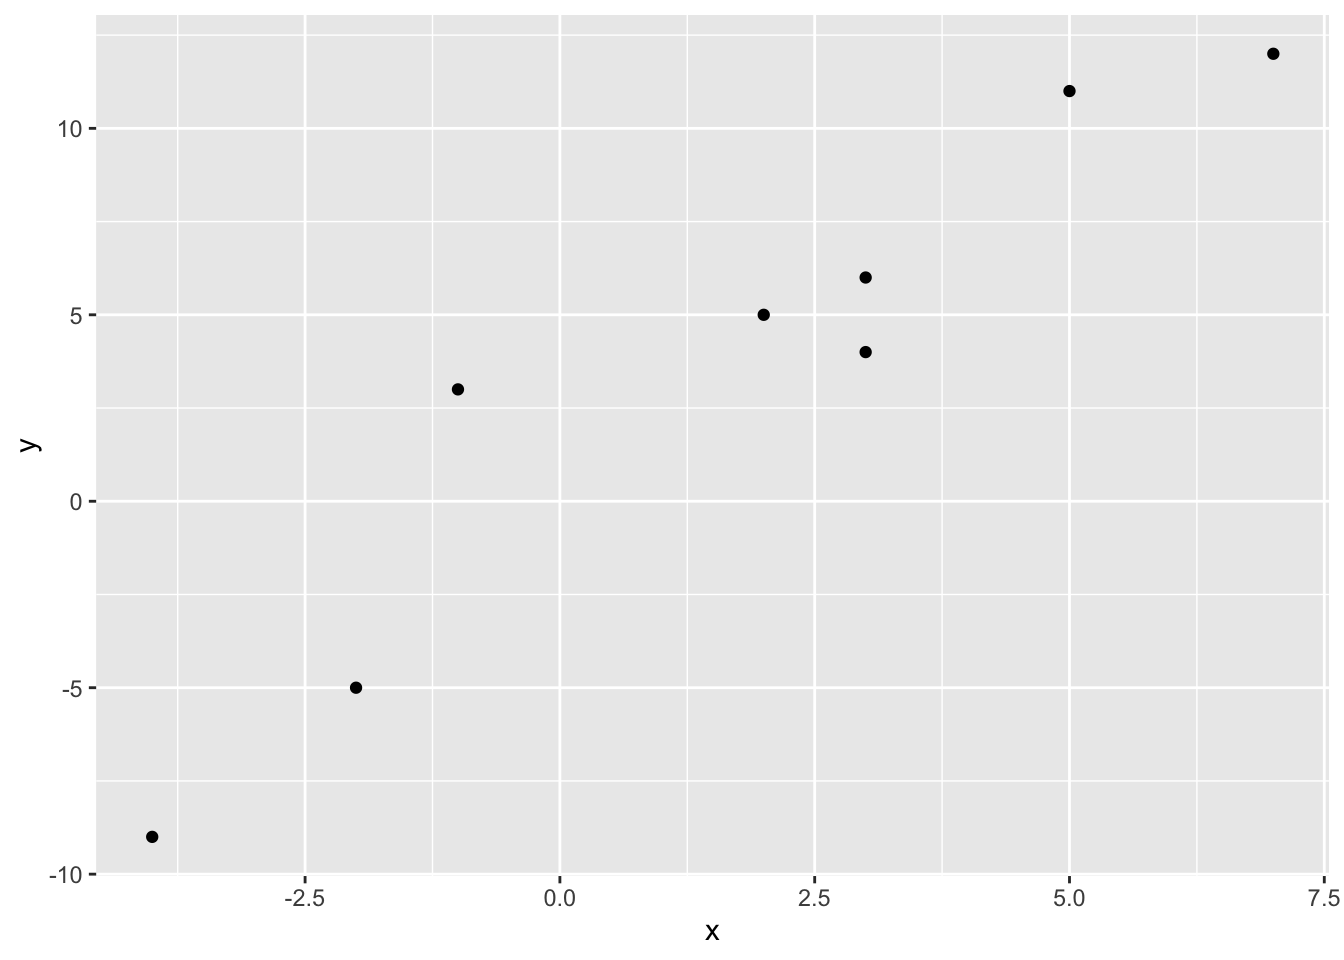
\includegraphics{multivariable-math_files/figure-latex/unnamed-chunk-227-1.pdf}
We can solve for the coefficients \texttt{beta} using the linear project theorem

\begin{Shaded}
\begin{Highlighting}[]
\NormalTok{beta <-}\StringTok{ }\KeywordTok{solve}\NormalTok{(}\KeywordTok{t}\NormalTok{(X) }\OperatorTok\StringTok{ }\NormalTok{X) }\OperatorTok\StringTok{ }\KeywordTok{t}\NormalTok{(X) }\OperatorTok\StringTok{ }\NormalTok{y}
\end{Highlighting}
\end{Shaded}

and using this solution, solve for the projection \(\mathbf{y}_{\mathcal{W}}\) of \(\mathbf{y}\) onto \(\mathbf{X}\)

\begin{Shaded}
\begin{Highlighting}[]
\NormalTok{y_W <-}\StringTok{ }\NormalTok{X }\OperatorTok\StringTok{ }\NormalTok{beta}
\end{Highlighting}
\end{Shaded}

Plotting the projection \(\mathbf{y}_{\mathcal{W}}\) gives

\begin{Shaded}
\begin{Highlighting}[]
\CommentTok{# The first column is a basis for a constant term (the intercept)}
\KeywordTok{data.frame}\NormalTok{(}\DataTypeTok{x =}\NormalTok{ X[, }\DecValTok{2}\NormalTok{], }\DataTypeTok{y =}\NormalTok{ y, }\DataTypeTok{y_W =}\NormalTok{ y_W) }\OperatorTok\StringTok{ }
\StringTok{    }\KeywordTok{ggplot}\NormalTok{(}\KeywordTok{aes}\NormalTok{(}\DataTypeTok{x =}\NormalTok{ x, }\DataTypeTok{y =}\NormalTok{ y)) }\OperatorTok{+}
\StringTok{    }\KeywordTok{geom_point}\NormalTok{() }\OperatorTok{+}
\StringTok{    }\KeywordTok{geom_line}\NormalTok{(}\KeywordTok{aes}\NormalTok{(}\DataTypeTok{x =}\NormalTok{ x, }\DataTypeTok{y =}\NormalTok{ y_W))}
\end{Highlighting}
\end{Shaded}

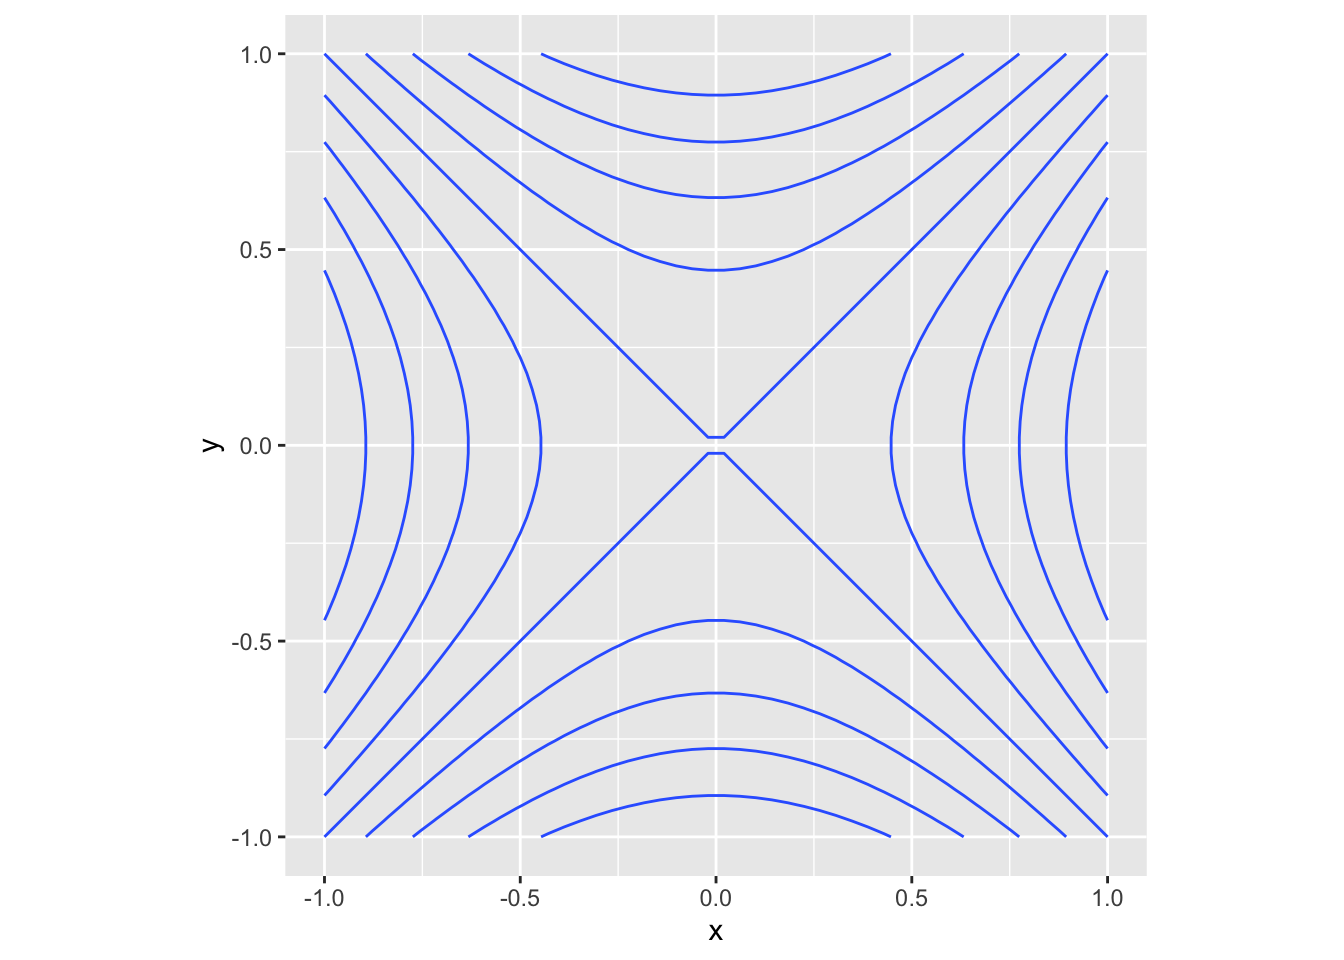
\includegraphics{multivariable-math_files/figure-latex/unnamed-chunk-230-1.pdf}
The complement of the project (called the \textbf{residuals} in statistics) is given by \(\mathbf{y}_{\mathcal{W}^\perp} = \mathbf{y} - \mathbf{y}_{\mathcal{W}}\)

\begin{Shaded}
\begin{Highlighting}[]
\NormalTok{y_W_perp <-}\StringTok{ }\NormalTok{y }\OperatorTok{-}\StringTok{ }\NormalTok{y_W}
\end{Highlighting}
\end{Shaded}

and can be visualized as the orthogonal projection using segments

\begin{Shaded}
\begin{Highlighting}[]
\CommentTok{# The first column is a basis for a constant term (the intercept)}
\KeywordTok{data.frame}\NormalTok{(}\DataTypeTok{x =}\NormalTok{ X[, }\DecValTok{2}\NormalTok{], }\DataTypeTok{y =}\NormalTok{ y, }\DataTypeTok{y_W =}\NormalTok{ y_W) }\OperatorTok\StringTok{ }
\StringTok{    }\KeywordTok{ggplot}\NormalTok{(}\KeywordTok{aes}\NormalTok{(}\DataTypeTok{x =}\NormalTok{ x, }\DataTypeTok{y =}\NormalTok{ y)) }\OperatorTok{+}
\StringTok{    }\KeywordTok{geom_point}\NormalTok{() }\OperatorTok{+}
\StringTok{    }\KeywordTok{geom_line}\NormalTok{(}\KeywordTok{aes}\NormalTok{(}\DataTypeTok{x =}\NormalTok{ x, }\DataTypeTok{y =}\NormalTok{ y_W)) }\OperatorTok{+}
\StringTok{    }\KeywordTok{geom_segment}\NormalTok{(}\KeywordTok{aes}\NormalTok{(}\DataTypeTok{x =}\NormalTok{ x, }\DataTypeTok{y =}\NormalTok{ y_W, }\DataTypeTok{xend =}\NormalTok{ x, }\DataTypeTok{yend =}\NormalTok{ y_W }\OperatorTok{+}\StringTok{ }\NormalTok{y_W_perp), }\DataTypeTok{color =} \StringTok{"blue"}\NormalTok{)}
\end{Highlighting}
\end{Shaded}

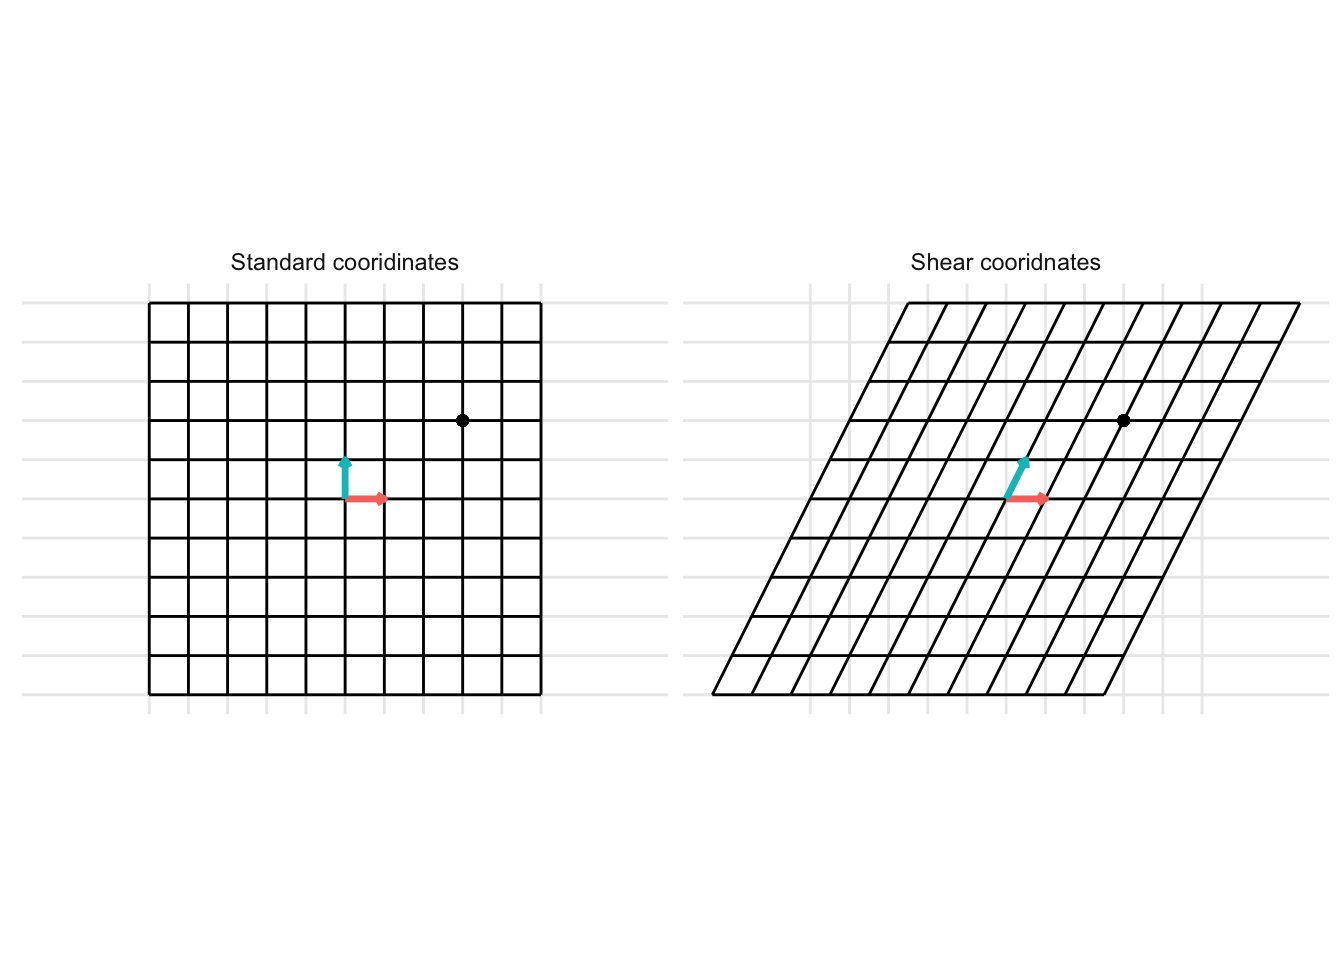
\includegraphics{multivariable-math_files/figure-latex/unnamed-chunk-232-1.pdf}
Recall that the orthogonal projection gives the ``closest'' vector \(\mathbf{y}_W\) to \(\mathbf{y}\) that is in the subspace \(\mathcal{W}\) that is the span of the column space of \(\mathbf{X}\). See \url{https://www.enchufa2.es/archives/least-squares-as-springs-the-shiny-app.html} for an example.

\hypertarget{graphs-and-limits}{%
\chapter{Graphs and Limits}\label{graphs-and-limits}}

\begin{Shaded}
\begin{Highlighting}[]
\KeywordTok{library}\NormalTok{(tidyverse)}
\KeywordTok{library}\NormalTok{(dasc2594)}
\KeywordTok{set.seed}\NormalTok{(}\DecValTok{2021}\NormalTok{)}
\end{Highlighting}
\end{Shaded}

Here we start a transition to topics in vector calculus. We will start with a discussion of functions of two variables (although the functions are not assumed to be linear). We define a function of two variables explicitly as \(z = f(x, y)\).

\begin{definition}
Like with linear functions, we can define the domain and range for general functions of two variables. A function \(f(x, y)\) assigns each point \((x, y)\) in some \textbf{domain} \(\mathcal{D}\) in \(\mathcal{R}^2\) to a unique number \(z\) in a subset of \(\mathcal{R}\). The set of inputs \(\mathcal{D}\) is called the \textbf{domain} of the function and the \textbf{range} is the set of real numbers \(z\) that are the output of the function over all the inputs in \(\mathcal{D}\)
\end{definition}

\begin{example}

Let \(f(x, y) = \sqrt{1 - x^2 - y^2}\).

\begin{itemize}
\item
  The domain of \(f\) is the set of points \((x, y)\) such that \(x^2 + y^2 \leq 1\) which is the unit circle (\textbf{draw picture}).
\item
  The range is the unit interval \([0, 1]\)
\end{itemize}

\end{example}

\hypertarget{graphs-and-level-curves}{%
\section{Graphs and level curves}\label{graphs-and-level-curves}}

\begin{example}
The parabola

Consider the function of two variables
\[
\begin{aligned}
f(x, y) = x^2 + y^2
\end{aligned}
\]
which defines the surface
\includegraphics{multivariable-math_files/figure-latex/unnamed-chunk-234-1.pdf}
The 3-dimensional surface can be represented in 2-dimensions using level curves (think of a topographic map)

\begin{Shaded}
\begin{Highlighting}[]
\KeywordTok{data.frame}\NormalTok{(}\KeywordTok{expand.grid}\NormalTok{(x, y)) }\OperatorTok
\StringTok{    }\KeywordTok{rename}\NormalTok{(}\DataTypeTok{x =}\NormalTok{ Var1, }\DataTypeTok{y =}\NormalTok{ Var2) }\OperatorTok
\StringTok{    }\KeywordTok{mutate}\NormalTok{(}\DataTypeTok{z =} \KeywordTok{parabola}\NormalTok{(x, y)) }\OperatorTok
\StringTok{    }\KeywordTok{ggplot}\NormalTok{(}\KeywordTok{aes}\NormalTok{(}\DataTypeTok{x =}\NormalTok{ x, }\DataTypeTok{y =}\NormalTok{ y, }\DataTypeTok{z =}\NormalTok{ z)) }\OperatorTok{+}
\StringTok{    }\KeywordTok{geom_contour}\NormalTok{() }\OperatorTok{+}
\StringTok{    }\KeywordTok{coord_fixed}\NormalTok{(}\DataTypeTok{ratio =} \DecValTok{1}\NormalTok{)}
\end{Highlighting}
\end{Shaded}

\includegraphics{multivariable-math_files/figure-latex/unnamed-chunk-235-1.pdf}
where each curve in the (x, y) plane has exactly the same value of \(f(x, y)\). Alternatively, this can be represented using filled level curves

\begin{Shaded}
\begin{Highlighting}[]
\KeywordTok{data.frame}\NormalTok{(}\KeywordTok{expand.grid}\NormalTok{(x, y)) }\OperatorTok
\StringTok{    }\KeywordTok{rename}\NormalTok{(}\DataTypeTok{x =}\NormalTok{ Var1, }\DataTypeTok{y =}\NormalTok{ Var2) }\OperatorTok
\StringTok{    }\KeywordTok{mutate}\NormalTok{(}\DataTypeTok{z =} \KeywordTok{parabola}\NormalTok{(x, y)) }\OperatorTok
\StringTok{    }\KeywordTok{ggplot}\NormalTok{(}\KeywordTok{aes}\NormalTok{(}\DataTypeTok{x =}\NormalTok{ x, }\DataTypeTok{y =}\NormalTok{ y, }\DataTypeTok{z =}\NormalTok{ z)) }\OperatorTok{+}
\StringTok{    }\KeywordTok{geom_contour_filled}\NormalTok{() }\OperatorTok{+}
\StringTok{    }\KeywordTok{coord_fixed}\NormalTok{(}\DataTypeTok{ratio =} \DecValTok{1}\NormalTok{)}
\end{Highlighting}
\end{Shaded}

\includegraphics{multivariable-math_files/figure-latex/unnamed-chunk-236-1.pdf}
Notice that although the original parabola was continuous, these 2-d representations simplify the diagram by representing the contours as discrete values.
\end{example}

\begin{example}
A saddle function

Consider the function of two variables
\[
\begin{aligned}
f(x, y) = x^2 - y^2
\end{aligned}
\]
which defines the surface
\includegraphics{multivariable-math_files/figure-latex/unnamed-chunk-237-1.pdf}
The 3-dimensional surface can be represented in 2-dimensions using level curves (think of a topographic map)

\begin{Shaded}
\begin{Highlighting}[]
\KeywordTok{data.frame}\NormalTok{(}\KeywordTok{expand.grid}\NormalTok{(x, y)) }\OperatorTok
\StringTok{    }\KeywordTok{rename}\NormalTok{(}\DataTypeTok{x =}\NormalTok{ Var1, }\DataTypeTok{y =}\NormalTok{ Var2) }\OperatorTok
\StringTok{    }\KeywordTok{mutate}\NormalTok{(}\DataTypeTok{z =} \KeywordTok{saddle}\NormalTok{(x, y)) }\OperatorTok
\StringTok{    }\KeywordTok{ggplot}\NormalTok{(}\KeywordTok{aes}\NormalTok{(}\DataTypeTok{x =}\NormalTok{ x, }\DataTypeTok{y =}\NormalTok{ y, }\DataTypeTok{z =}\NormalTok{ z)) }\OperatorTok{+}
\StringTok{    }\KeywordTok{geom_contour}\NormalTok{() }\OperatorTok{+}
\StringTok{    }\KeywordTok{coord_fixed}\NormalTok{(}\DataTypeTok{ratio =} \DecValTok{1}\NormalTok{)}
\end{Highlighting}
\end{Shaded}

\includegraphics{multivariable-math_files/figure-latex/unnamed-chunk-238-1.pdf}
where each curve in the (x, y) plane has exactly the same value of \(f(x, y)\). Alternatively, this can be represented using filled level curves

\begin{Shaded}
\begin{Highlighting}[]
\KeywordTok{data.frame}\NormalTok{(}\KeywordTok{expand.grid}\NormalTok{(x, y)) }\OperatorTok
\StringTok{    }\KeywordTok{rename}\NormalTok{(}\DataTypeTok{x =}\NormalTok{ Var1, }\DataTypeTok{y =}\NormalTok{ Var2) }\OperatorTok
\StringTok{    }\KeywordTok{mutate}\NormalTok{(}\DataTypeTok{z =} \KeywordTok{saddle}\NormalTok{(x, y)) }\OperatorTok
\StringTok{    }\KeywordTok{ggplot}\NormalTok{(}\KeywordTok{aes}\NormalTok{(}\DataTypeTok{x =}\NormalTok{ x, }\DataTypeTok{y =}\NormalTok{ y, }\DataTypeTok{z =}\NormalTok{ z)) }\OperatorTok{+}
\StringTok{    }\KeywordTok{geom_contour_filled}\NormalTok{() }\OperatorTok{+}
\StringTok{    }\KeywordTok{coord_fixed}\NormalTok{(}\DataTypeTok{ratio =} \DecValTok{1}\NormalTok{)}
\end{Highlighting}
\end{Shaded}

\includegraphics{multivariable-math_files/figure-latex/unnamed-chunk-239-1.pdf}
Notice that although the original saddle was continuous, these 2-d representations simplify the diagram by representing the contours as discrete values.
\end{example}

\hypertarget{limits}{%
\section{Limits}\label{limits}}

For functions of several variables, we have to define limits and continuity for these multivariable settings. For now, we focus on two variable functions as the multivariable case follows similar from the two variable case.

Let \(P(x, y) \rightarrow P_0(a, b)\) be a path in the \(x-y\) plane that starts at the point \(P(x, y)\) and ends at the point \(P_0(a, b)\) with coordinates \((a, b)\). Thus, we can understand the limit as the fixed value of \(f(x, y)\) for which all paths that connect the points \(P(x, y)\) that are ``close'' to \(P_0(a, b)\) converge to.

For one-dimensional limits, ``close'' was defined as distance. Thus, for multivariable functions, ``close'' is defined as the Euclidean distance defined by a ``ball'' of radius \(\delta\) and the limits examines the function output as the radius \(\delta\) goes to 0.

Recall that the distance \(dist((x, y), (a, b))\) between two points \((x, y)\) and \((a, b)\) is
\[
\begin{aligned}
dist((x, y), (a, b)) = \sqrt{(x-a)^2 + (y-b)^2}
\end{aligned}
\]

** Draw images**

\begin{definition}[Limit of a function of two variables]
The function f(x, y) has limit \(L\) as \(P(x, y) \rightarrow P_0(a, b)\), written
\[
\begin{aligned}
\lim_{(x, y) \rightarrow (a, b)} f(x, y) = \lim_{P \rightarrow P_0} f(x, y) = L,
\end{aligned}
\]
if, for any \(\epsilon > 0\) (the radius of the ball that defines the ``closeness'' of the point), there exists a \(\delta > 0\) such that
\[
\begin{aligned}
|f(x, y) - L| < \epsilon
\end{aligned}
\]
whenever \((x, y)\) is in the domain of \(f\) and
\[
\begin{aligned}
0 < \sqrt{(x-a)^2 + (y-b)^2} < \delta.
\end{aligned}
\]
\end{definition}

In the definition, as the value of \(\delta\) is getting smaller, the distance between the set of points \(P(x, y)\) within radius \(\delta\) of the point \(P_0(a, b)\) is getting smaller. As a consequence, the limit in the definition above exists only if \(f(x, y)\) approaches the value \(L\) along \textbf{all possible paths} in the domain of \(f\).

\begin{example}
In class notes
* \textbf{Future work: write out hand-written examples}
\end{example}

\begin{theorem}

Let \(L\) and \(M\) be real numbers and let \(\lim_{(x, y) \rightarrow (a, b)}f(x, y) = L\) and \(\lim_{(x, y) \rightarrow (a, b)}g(x, y) = M\) for functions \(f(x, y)\) and \(g(x, y)\). Let \(c\) be a constant and \(n>0\), then:

\begin{enumerate}
\def\labelenumi{\arabic{enumi})}
\item
  \textbf{Sum of limits:}
  \[
  \begin{aligned}
  \lim_{(x, y) \rightarrow (a, b)} \left( f(x, y) + g(x, y) \right) = L + M
  \end{aligned}
  \]
\item
  \textbf{Difference of limits:}
  \[
  \begin{aligned}
  \lim_{(x, y) \rightarrow (a, b)} \left( f(x, y) - g(x, y) \right) = L - M
  \end{aligned}
  \]
\item
  \textbf{Scalar multiple of the limit:}
  \[
  \begin{aligned}
  \lim_{(x, y) \rightarrow (a, b)} c f(x, y) = c L
  \end{aligned}
  \]
\item
  \textbf{Product of limits:}
  \[
  \begin{aligned}
  \lim_{(x, y) \rightarrow (a, b)} f(x, y) g(x, y) = LM
  \end{aligned}
  \]
\item
  \textbf{Quotient of limits:} As long as \(M>0\) we have
  \[
  \begin{aligned}
  \lim_{(x, y) \rightarrow (a, b)} \frac{f(x, y)}{g(x, y)} = \frac{L}{M}
  \end{aligned}
  \]
\item
  \textbf{Power of the limit:}
  \[
  \begin{aligned}
  \lim_{(x, y) \rightarrow (a, b)} f(x, y)^n = L^n
  \end{aligned}
  \]
\item
  \textbf{Root of the limit:} If \(n\) is even, we assume \(L > 0\)
  \[
  \begin{aligned}
  \lim_{(x, y) \rightarrow (a, b)} f(x, y)^{1/n} = L^{1/n}
  \end{aligned}
  \]
\end{enumerate}

\end{theorem}

\begin{example}
Use the rules above to evaluate the limit \(\lim_{(x, y) \rightarrow (2, 3)} 4x^3y + \sqrt{xy}\)
\end{example}

\hypertarget{boundary-points}{%
\subsection{Boundary points}\label{boundary-points}}

\begin{definition}

Define a region \(\mathcal{D}\) in \(\mathcal{R}^2\).

\begin{itemize}
\item
  An \textbf{interior} point \(P\) of \(\mathcal{D}\) is a point that lies entirely in the region \(\mathcal{D}\). Mathematically, a point \(P\) is an interior point of \(\mathcal{D}\) if it is possible to define a ball of radius \(\epsilon>0\) centered at \(P\) such that this ball only contains points within \(\mathcal{D}\).
\item
  A \textbf{boundary} point \(P\) of \(\mathcal{D}\) is a point that lies on the edge of the region \(\mathcal{D}\). Mathematically, a point \(P\) is an boundary point of \(\mathcal{D}\) if every ball of radius \(\epsilon>0\) centered at \(P\) contains at least one point in \(\mathcal{D}\) and one point outside \(\mathcal{D}\).
\end{itemize}

\end{definition}

\begin{example}
Let \(f(x, y) = \sqrt{1 - x^2 - y^2}\). The boundary points are all the points on the unit circle an the interior points are all the points on the interior of the unit disk. \textbf{draw picture}
\end{example}

\begin{definition}
A region \(\mathcal{D}\) is said to be \textbf{open} if it only contains interior points (i.e., \(\mathcal{D}\) has no boundary points). A region \(\mathcal{D}\) is said to be \textbf{closed} if the region contains all its boundary points.
\end{definition}

\textbf{Figure: limit paths along the boundary}

\begin{example}
Consider the \(\lim_{(x, y) \rightarrow (4, 4)} \frac{x^2 - y^2}{x - y}\). Because the point \((4, 4)\) is not a valid point in the domain (can't divide by \(4-4=0\)), the point \((4, 4)\) is a boundary point of the domain. The boundary of the domain that is not contained in the domain is the set of points \(x = y\). Assuming we are not taking a path along the boundary, we know that \(x \neq y\) in the interior of the domain. Hence,
\[
\begin{aligned}
\lim_{(x, y) \rightarrow (4, 4)} \frac{x^2 - y^2}{x - y} & = \lim_{(x, y) \rightarrow (4, 4)} \frac{(x - y)(x + y)}{x - y} \\
& = \lim_{(x, y) \rightarrow (4, 4)} x + y  = 4 + 4 = 8\\
\end{aligned}
\]
for all paths that do not cross the line \(y = x\).
\end{example}

\begin{example}
\textbf{nonexistence of limit in class}
\end{example}

\hypertarget{continuity}{%
\section{Continuity}\label{continuity}}

A very important property of functions is continuity. In a general sense, a function is continuous if two nearby input values result in nearby output values. As a graph, this means that there are no hops, skips, or jumps.

\begin{definition}

The function \(f(x, y)\) is said to be continuous at the point \((a, b)\) if the following are true

\begin{enumerate}
\def\labelenumi{\arabic{enumi})}
\item
  \(f(a, b)\) is defined at \((a, b)\)
\item
  \(\lim_{(x, y) \rightarrow (a, b)} f(x, y)\) exists
\item
  \(\lim_{(x, y) \rightarrow (a, b)} f(x, y) = f(a, b)\)
\end{enumerate}

\end{definition}

\begin{example}
\textbf{checking continuity in class}
\(f(x, y) = \begin{cases} \frac{x^2 - y^2}{x - y} & \mbox{ if } x \neq y \\ x + y & \mbox{ if } x = y \\ \end{cases}\)
\end{example}

\hypertarget{partial-derivatives}{%
\chapter{Partial Derivatives}\label{partial-derivatives}}

\begin{Shaded}
\begin{Highlighting}[]
\KeywordTok{library}\NormalTok{(tidyverse)}
\KeywordTok{library}\NormalTok{(plotly)}
\KeywordTok{library}\NormalTok{(dasc2594)}
\KeywordTok{set.seed}\NormalTok{(}\DecValTok{2021}\NormalTok{)}
\end{Highlighting}
\end{Shaded}

Recall that for a function of one variable, the derivative gives the rate of change of the function with respect to that variable. The function \(f(x)\) has an instantaneous rate of change \(\frac{d}{dx}f(x)\), assuming the derivative \(\frac{d}{dx}f(x)\) exists.

This concept can be extended to functions of multivariables where we now have to specify a direction in which the function changes. For example, consider a mountain which is very steep in the north/south direction but is much less steep in the east/west direction. Thus, the directional derivative in the north/south direction will have a larger absolute value (higher rate of change) than the directional derivative in the east/west direction.

For example, consider the function

\begin{Shaded}
\begin{Highlighting}[]
\NormalTok{mountain <-}\StringTok{ }\ControlFlowTok{function}\NormalTok{(x, y) \{}
    \DecValTok{4} \OperatorTok{-}\StringTok{ }\DecValTok{9} \OperatorTok{*}\StringTok{ }\NormalTok{x}\OperatorTok{^}\DecValTok{2} \OperatorTok{-}\StringTok{ }\NormalTok{y}\OperatorTok{^}\DecValTok{2}
\NormalTok{\}}
\NormalTok{dat <-}\StringTok{ }\KeywordTok{expand_grid}\NormalTok{(}\DataTypeTok{x =} \KeywordTok{seq}\NormalTok{(}\OperatorTok{-}\DecValTok{4}\NormalTok{, }\DecValTok{4}\NormalTok{, }\DataTypeTok{length.out =} \DecValTok{20}\NormalTok{), }\DataTypeTok{y =} \KeywordTok{seq}\NormalTok{(}\OperatorTok{-}\DecValTok{4}\NormalTok{, }\DecValTok{4}\NormalTok{, }\DataTypeTok{length.out =} \DecValTok{20}\NormalTok{)) }\OperatorTok
\StringTok{    }\KeywordTok{mutate}\NormalTok{(}\DataTypeTok{z =} \KeywordTok{mountain}\NormalTok{(x, y))}

\NormalTok{dat }\OperatorTok
\StringTok{    }\KeywordTok{ggplot}\NormalTok{(}\KeywordTok{aes}\NormalTok{(}\DataTypeTok{x =}\NormalTok{ x, }\DataTypeTok{y =}\NormalTok{ y, }\DataTypeTok{z =}\NormalTok{ z)) }\OperatorTok{+}
\StringTok{    }\KeywordTok{geom_contour}\NormalTok{() }\OperatorTok{+}
\StringTok{    }\KeywordTok{coord_fixed}\NormalTok{(}\DataTypeTok{ratio =} \DecValTok{1}\NormalTok{)}
\end{Highlighting}
\end{Shaded}

\includegraphics{multivariable-math_files/figure-latex/unnamed-chunk-242-1.pdf}

\begin{Shaded}
\begin{Highlighting}[]
\KeywordTok{plot_ly}\NormalTok{(}\DataTypeTok{z =} \KeywordTok{matrix}\NormalTok{(dat}\OperatorTok{$}\NormalTok{z, }\DecValTok{20}\NormalTok{, }\DecValTok{20}\NormalTok{)) }\OperatorTok
\StringTok{    }\KeywordTok{add_surface}\NormalTok{(}
        \DataTypeTok{contours =} \KeywordTok{list}\NormalTok{(}
            \DataTypeTok{z =} \KeywordTok{list}\NormalTok{(}
                \DataTypeTok{show=}\OtherTok{TRUE}\NormalTok{,}
                \DataTypeTok{usecolormap=}\OtherTok{TRUE}\NormalTok{,}
                \DataTypeTok{highlightcolor=}\StringTok{"#ff0000"}\NormalTok{,}
                \DataTypeTok{project=}\KeywordTok{list}\NormalTok{(}\DataTypeTok{z=}\OtherTok{TRUE}\NormalTok{)}
\NormalTok{            )}
\NormalTok{        )}
\NormalTok{    )}
\end{Highlighting}
\end{Shaded}

\includegraphics[width=1\linewidth]{./webshot-images/contour}
Note that the partial derivative asks the question ``What is the rate of change of one variable holding all the other variables constant?'' Thus, the question can be phrased as what is the derivative of the function \(f(x, y)\) at the point \((a, b)\) where we only let one variable change? To make the notation of a partial derivative clear, a special symbol is used where \(\frac{\partial}{\partial x}\) is the partial derivative with respect to the \(x\) variable (holding the y variable constant).

\textbf{draw surfaces with marginal slices}

\begin{definition}
\protect\hypertarget{def:partial}{}\label{def:partial}The partial derivative of the function \(f(x, y)\) with respect to \(x\) at the point \((a, b)\) is
\[
\begin{aligned}
\frac{\partial}{\partial x} f(x, y) = f_x(x, y) & = \lim_{h \rightarrow 0} \frac{f(a + h, b) - f(a, b)} {h}.
\end{aligned}
\]

The partial derivative of the function \(f(x, y)\) with respect to \(y\) at the point \((a, b)\) is
\[
\begin{aligned}
\frac{\partial}{\partial y} f(x, y) = f_y(x, y) & = \lim_{h \rightarrow 0} \frac{f(a, b + h) - f(a, b)} {h},
\end{aligned}
\]
as long as these limits exist.
\end{definition}

\begin{example}
\textbf{partial derivatives using limit definition}
\end{example}

\begin{example}
Let \(f(x, y) = 3x^2 - 4 y^3 + 3\), Compute \(\frac{\partial}{\partial x}f(x, y)\) and \(\frac{\partial}{\partial y}f(x, y)\). Then evaluate each derivative at \((-2, 3)\).
\end{example}

Notice that you can find partial derivatives by holding all the other variables constant and then finding the equivalent univariate derivative.

\hypertarget{higher-order-partial-derivatives}{%
\section{Higher-order partial derivatives}\label{higher-order-partial-derivatives}}

We can calculate the partial derivatives of partial derivatives. The derivatives could be with respect to the same variable repeatedly or the derivatives could be with respect to different variables in which case we call these \textbf{mixed partial derivatives}. Notation for higher order partial derivatives is \(\frac{\partial^2}{\partial x \partial y} f(x, y) = f_{xy}(x, y)\) which says first take the partial derivative of with respect to \(y\) then take the partial derivative with respect to \(x\). The possible sets of second-order partial derivatives for functions of two variables are shown in the table below

\begin{longtable}[]{@{}ll@{}}
\toprule
\begin{minipage}[b]{0.47\columnwidth}\raggedright
Notation 1\strut
\end{minipage} & \begin{minipage}[b]{0.47\columnwidth}\raggedright
Notation 2\strut
\end{minipage}\tabularnewline
\midrule
\endhead
\begin{minipage}[t]{0.47\columnwidth}\raggedright
\(\frac{\partial}{\partial x}\frac{\partial}{\partial x} f(x, y) = \frac{\partial^2}{\partial x^2} f(x, y)\)\strut
\end{minipage} & \begin{minipage}[t]{0.47\columnwidth}\raggedright
\(f_{xx}(x, y)\)\strut
\end{minipage}\tabularnewline
\begin{minipage}[t]{0.47\columnwidth}\raggedright
\(\frac{\partial}{\partial y}\frac{\partial}{\partial y} f(x, y) = \frac{\partial^2}{\partial y^2} f(x, y)\)\strut
\end{minipage} & \begin{minipage}[t]{0.47\columnwidth}\raggedright
\(f_{yy}(x, y)\)\strut
\end{minipage}\tabularnewline
\begin{minipage}[t]{0.47\columnwidth}\raggedright
\(\frac{\partial}{\partial x}\frac{\partial}{\partial y} f(x, y) = \frac{\partial^2}{\partial x \partial y} f(x, y)\)\strut
\end{minipage} & \begin{minipage}[t]{0.47\columnwidth}\raggedright
\(f_{xy}(x, y)\)\strut
\end{minipage}\tabularnewline
\begin{minipage}[t]{0.47\columnwidth}\raggedright
\(\frac{\partial}{\partial y}\frac{\partial}{\partial x} f(x, y) = \frac{\partial^2}{\partial y \partial x} f(x, y)\)\strut
\end{minipage} & \begin{minipage}[t]{0.47\columnwidth}\raggedright
\(f_{yx}(x, y)\)\strut
\end{minipage}\tabularnewline
\bottomrule
\end{longtable}

\begin{example}
Find the four second-order partial derivatives of \(f(x, y) = 3x^2y^3 + 4xy - 3x^2\)
\end{example}

Note that the order in which mixed partial derivatives are taken can sometimes change the result. However, it is often the case that the order of the partial derivatives can be switched.

\begin{theorem}
Let the function \(f(x, y)\) be defined on an open domain \(\mathcal{D}\) of \(\mathcal{R}^2\) and assume that \(f_{xy}\) and \(f_{yx}\) are continuous over the domain \(\mathcal{D}\). Then, \(f_{xy} = f_{yx}\) for all points in the domain \(\mathcal{D}\).
\end{theorem}

Many of the commonly used functional forms in data science meet the criteria above. Thus, for many of the commonly used functions in data science, the order of evaluation of partial derivatives often does not matter. In practice, it is always good practice to verify this though.

\hypertarget{the-chain-rule}{%
\chapter{The chain rule}\label{the-chain-rule}}

\begin{Shaded}
\begin{Highlighting}[]
\KeywordTok{library}\NormalTok{(tidyverse)}
\KeywordTok{library}\NormalTok{(plotly)}
\KeywordTok{library}\NormalTok{(dasc2594)}
\KeywordTok{set.seed}\NormalTok{(}\DecValTok{2021}\NormalTok{)}
\end{Highlighting}
\end{Shaded}

Recall the univariate chain rule: If \(y = f(x)\) is a function of \(x\) and \(z = g(y)\) is a function of \(y\), a question of interest is "What is the change in \(z\) relative to change in \(x\)?

We can write \(z = g(y) = g(f(x))\) and using this notation, the change in \(z\) with respect to the variable \(x\) is \(\frac{dz}{dx} = \frac{dz}{dy}\frac{dy}{dx} = \frac{df(y)}{dy}\frac{dg(x)}{dx}\). Written in functional form
\[
\begin{aligned}
(g(f(x)))' = (g \circ f)'(x) = g'(f(x)) f'(x)
\end{aligned}
\]

\begin{example}
Let \(z = f(y) = y^3\) and let \(y = g(x) = e^{x}\) what is \(\frac{dz}{dx}\)?
\end{example}

\hypertarget{the-chain-rule-with-one-independent-variable}{%
\section{The chain rule with one independent variable}\label{the-chain-rule-with-one-independent-variable}}

\textbf{Drawing in class}

\begin{definition}[Chain rule for one independent variable]

Let \(z\) be a differentiable function of two variables \(x\) and \(y\) so that \(z = f(x, y)\) and let \(x=g(t)\) be a function of \(t\) and \(y=h(t)\) a function of \(t\). Written in functional form, \(z\) can be written as \(z = f(x, y) = f(g(t), h(t))\), with \(x=g(t)\) and \(y=h(t)\). Then we can define the derivative of \(z\) with respect to \(t\) as
\[
\begin{aligned}
\frac{dz}{dt} = \frac{\partial z}{ \partial x}\frac{dx}{dt} + \frac{\partial z}{\partial y}\frac{dy}{dt}
\end{aligned}
\]

\begin{itemize}
\item
  For the definition above, we have the dependent variable \(z\) and we have \textbf{intermediate variables} \(x\) and \(y\).
\item
  Notice in the definition above that there is a mix of partial derivatives (\(\partial\)) and ordinary derivatives (\(d\)).
\end{itemize}

\end{definition}

\begin{example}
Let \(z = x^2 + e^y\) and let \(x = \cos(t)\) and \(y = \sin(t)\)
\end{example}

The results from above can also be extended to have more than two intermediate variables.

\textbf{Draw picture}

\hypertarget{the-chain-rule-with-several-independent-variables}{%
\section{The chain rule with several independent variables}\label{the-chain-rule-with-several-independent-variables}}

Often, functions will have more than one independent variables.

\begin{definition}[Chain rule for two independent variables]
Let \(z\) be a differentiable function of two variables \(x\) and \(y\) so that \(z = f(x, y)\) and let \(x=g(t, s)\) be a function of \(s\) and \(t\) and \(y=h(s, t)\) a function of \(s\) and \(t\). Written in functional form, \(z\) can be written as \(z = f(x, y) = f(g(s, t), h(s, t))\), with \(x=g(s, t)\) and \(y=h(s, t)\). Then we can define the partial derivative of \(z\) with respect to \(s\) as
\[
\begin{aligned}
\frac{\partial z}{\partial s} = \frac{\partial z}{ \partial x}\frac{\partial x}{\partial s} + \frac{\partial z}{\partial y}\frac{\partial y}{\partial s}
\end{aligned}
\]
the partial derivative of \(z\) with respect to \(t\) as
\[
\begin{aligned}
\frac{\partial z}{\partial t} = \frac{\partial z}{ \partial x}\frac{\partial x}{\partial t} + \frac{\partial z}{\partial y}\frac{\partial y}{\partial t}
\end{aligned}
\]
\end{definition}

\begin{example}
Let \(z = f(x, y) = x^2 e^y\) and let \(x = 2s - t\) and \(y = 4s^3-3t^2\)
\end{example}

\hypertarget{the-chain-rule-in-matrix-notation}{%
\section{The chain rule in matrix notation}\label{the-chain-rule-in-matrix-notation}}

To get a better understanding of the chain rule, it helps to show the chain rule using matrix notation. Using the matrix notation will enable you to apply the chain rule to any number of intermediate variables. For example, consider the extension of the definition for the chain rule of a function with one independent variable.

\begin{definition}[Matrix chain rule for one independent variable]
Let \(z\) be a differentiable function of two variables \(x\) and \(y\) so that \(z = f(x, y)\) and let \(x=g(t)\) be a function of \(t\) and \(y=h(t)\) a function of \(t\). Written in functional form, \(z\) can be written as \(z = f(x, y) = f(g(t), h(t))\), with \(x=g(t)\) and \(y=h(t)\). Then we can define the derivative of \(z\) with respect to \(t\) as
\[
\begin{aligned}
\frac{dz}{dt} = \frac{\partial z}{ \partial x}\frac{dx}{dt} + \frac{\partial z}{\partial y}\frac{dy}{dt}
\end{aligned}
\]

Written in matrix notation, this is
\[
\begin{aligned}
\frac{dz}{dt} = \begin{pmatrix} \frac{\partial z}{ \partial x} & \frac{\partial z}{\partial y} \end{pmatrix} \begin{pmatrix} \frac{dx}{dt} \\  \frac{dy}{dt} \end{pmatrix} = \frac{\partial z}{ \partial x}\frac{dx}{dt} + \frac{\partial z}{\partial y}\frac{dy}{dt}
\end{aligned}
\]
\end{definition}

The definition above for the chain rule with two variables is given by

\begin{definition}[Chain rule for two independent variables]
Let \(z\) be a differentiable function of two variables \(x\) and \(y\) so that \(z = f(x, y)\) and let \(x=g(t, s)\) be a function of \(s\) and \(t\) and \(y=h(s, t)\) a function of \(s\) and \(t\). Written in functional form, \(z\) can be written as \(z = f(x, y) = f(g(s, t), h(s, t))\), with \(x=g(s, t)\) and \(y=h(s, t)\). Then we can define the partial derivative of \(z\) with respect to \(s\) as
\[
\begin{aligned}
\frac{\partial z}{\partial s} = \frac{\partial z}{ \partial x}\frac{\partial x}{\partial s} + \frac{\partial z}{\partial y}\frac{\partial y}{\partial s}
\end{aligned}
\]
which, in matrix notation is
\[
\begin{aligned}
\frac{dz}{dt} = \begin{pmatrix} \frac{\partial z}{ \partial x} & \frac{\partial z}{\partial y} \end{pmatrix} \begin{pmatrix} \frac{\partial x}{\partial s} \\  \frac{\partial y}{\partial s} \end{pmatrix} = \frac{\partial z}{ \partial x}\frac{\partial x}{\partial s} + \frac{\partial z}{\partial y}\frac{\partial y}{\partial s}
\end{aligned}
\]

The partial derivative of \(z\) with respect to \(t\) as
\[
\begin{aligned}
\frac{\partial z}{\partial t} = \frac{\partial z}{ \partial x}\frac{\partial x}{\partial t} + \frac{\partial z}{\partial y}\frac{\partial y}{\partial t}
\end{aligned}
\]
which, in matrix notation is
\[
\begin{aligned}
\frac{dz}{dt} = \begin{pmatrix} \frac{\partial z}{ \partial x} & \frac{\partial z}{\partial y} \end{pmatrix} \begin{pmatrix} \frac{\partial x}{\partial t} \\  \frac{\partial y}{\partial t} \end{pmatrix} = \frac{\partial z}{ \partial x}\frac{\partial x}{\partial t} + \frac{\partial z}{\partial y}\frac{\partial y}{\partial t}
\end{aligned}
\]
\end{definition}

This use of matrix notation for derivatives will be useful in understanding the \textbf{gradient}.

\hypertarget{the-gradient-and-directional-derivatives}{%
\chapter{The gradient and directional derivatives}\label{the-gradient-and-directional-derivatives}}

\begin{Shaded}
\begin{Highlighting}[]
\KeywordTok{library}\NormalTok{(tidyverse)}
\KeywordTok{library}\NormalTok{(plotly)}
\KeywordTok{library}\NormalTok{(dasc2594)}
\KeywordTok{set.seed}\NormalTok{(}\DecValTok{2021}\NormalTok{)}
\end{Highlighting}
\end{Shaded}

Partial derivatives tell about how a rate of function changes in a particular direction (in the direction of a coordinate).

Think about trying to find the maximum of a real-valued function (finding the minimum is equivalent to finding the maximum of the negative value of the function). Finding the maximum of a function is analogous to hiking up a mountain and trying to find the highest peak.

Suppose you are standing on a mountain surface at the point \((x, y, z)\) in 3-dimensions where \(z = f(x, y)\) is the function that gives the height of the mountain at location \((x, y)\). If you are standing at the point \((a, b)\) in the \((x, y)\) coordinate system, you might want to get to the top of the mountain as quickly as possible. The direction that is the steepest uphill direction can be calculated using the concepts of the \textbf{directional derivative} and the \textbf{gradient}.

\begin{definition}[Directional Derivative]
Given a function \(f(x,y)\) that is differentiable at \((a, b)\) and a unit vector \(\mathbf{v} = \begin{pmatrix} v_1 \\ v_2 \end{pmatrix}\) in the \(x-y\) plane, the \textbf{directional derivative} of \(f\) at \((a, b)\) in the direction of \(\mathbf{v}\) is
\[
\begin{aligned}
D_{\mathbf{v}} f(a, b) = \lim_{h \rightarrow 0} \frac{f(a + h v_1, b + h v_2) - f(a, b)}{h}
\end{aligned}
\]
assuming the limit exists.
\end{definition}

To understand how the directional derivative relates to partial derivatives, in the definition above, let \(v_2 = 0\) and to make \(\mathbf{v}\) a unit vector, set \(v_1 = 1\) (\(\mathbf{v}\) is the standard basis vector \(\mathbf{e}_1\)). Then, the limit in the directional derivative definition above becomes
\[
\begin{aligned}
\lim_{h \rightarrow 0} \frac{f(a + h, b) - f(a, b)}{h}
\end{aligned}
\]
which is the definition for the partial derivative of \(f\) in the \(x\) direction \(f_x = \frac{\partial f}{\partial x}\) (Definition \ref{def:partial}). Likewise, letting \(\mathbf{v} = \mathbf{e}_2\), the standard basis vector in the y direction, gives the partial derivative in the y direction \(f_y = \frac{\partial f}{\partial y}\). Thus, one could pick any direction vector \(\mathbf{v}\) and then calculate the partial derivative in that direction.

Now observe that any line that goes through the point \((a, b)\) in the direction of the unit vector \(\mathbf{v} \in \mathcal{R}^2\) can be written as the set of points \(\{(x = a + s v_1, y = b + s v_2) | s \in \mathcal{R} \}\) which forms a line through the point \((a, b)\) in the direction of \(\mathbf{v}\). In this definition, the value \(s\) determines the length of the vector because \(\mathbf{v}\) is a unit vector. At \(s=0\), this definition corresponds to the point \((a, b)\) and as \(s\) increases, the points \((x, y)\) are the set of points along the line that are distance \(|s|\) away from \((a, b)\). Notice that this set defines a function \(g(s) = f(a + s v_1, b + s v_2) = f(x, y)\) which is a single variable function of the two inputs \(x\) and \(y\) of \(f(x, y)\). Given this definition, the directional derivative of \(f(x, y)\) in the direction of \(\mathbf{v}\) at the point \((a, b)\) is now given by

\[
\begin{aligned}
D_{\mathbf{v}} f(a, b) & = \frac{d}{ds}g(s)|_{s=0} \\
& = \frac{\partial f}{\partial x} \frac{dx}{ds} + \frac{\partial f}{\partial y} \frac{dy}{ds} |_{s=0} \\
& = f_x(a, b) v_1 + f_y(a, b) v_2 \\
& = \begin{pmatrix} f_x(a, b) & f_y(a, b) \end{pmatrix} \begin{pmatrix} v_1 \\ v_2 \end{pmatrix} \\
\end{aligned}
\]
which is the dot product of the vectors \(\begin{pmatrix} f_x(a, b) \\ f_y(a, b) \end{pmatrix}\) and \(\mathbf{v}\).

Notice that the vector \(\mathbf{v}\) is a unit vector and therefore the directional derivative is a weighted sum of the partial derivatives in the \(x\) and \(y\) directions weighted by the vector \(\mathbf{v}\) (weighted sums are sums where the coefficients sum to 1--in this case the sum is in the ``distance'' metric). As a consequence, we can find the directional derivative in any direction by changing the vector \(\mathbf{v}\).

\begin{definition}
\protect\hypertarget{def:directional-gradient}{}\label{def:directional-gradient}Let \(f(x, y)\) be a differentiable function at \((a, b)\) and \(\mathbf{v} = \begin{pmatrix} v_1 \\ v_2 \end{pmatrix}\) a unit vector in the \(xy\) plane. Then, the directional derivative of \(f\) at \((a, b)\) in the direction of \(\mathbf{v}\) is
\[
\begin{aligned}
D_{\mathbf{v}} f(a, b) & = \begin{pmatrix} \frac{\partial f(x, y)}{\partial x}|_{(x,y) = (a, b)} & \frac{\partial f(x, y)}{\partial y}|_{(x,y) = (a, b)} \end{pmatrix} \begin{pmatrix} v_1 \\ v_2 \end{pmatrix} \\
\end{aligned}
\]
\end{definition}

\begin{example}
Compute the directional derivative of \(f(x, y) = 3x^2 + y^2\) in the direction of \(\mathbf{u} = \begin{pmatrix} \frac{1}{\sqrt{3}}, \frac{\sqrt{2}}{\sqrt{3}} \end{pmatrix}\) and \(\mathbf{v} = \begin{pmatrix} \frac{1}{\sqrt{2}}, - \frac{1}{\sqrt{2}} \end{pmatrix}\) at the point \((2, 1)\).

\begin{itemize}
\tightlist
\item
  calculate the directional derivatives
\item
  graph the directional derivatives using contour plots and segments
\end{itemize}

\begin{Shaded}
\begin{Highlighting}[]
\CommentTok{# the function}
\NormalTok{target_fun <-}\StringTok{ }\ControlFlowTok{function}\NormalTok{(x, y) \{}
        \DecValTok{3} \OperatorTok{*}\StringTok{ }\NormalTok{x}\OperatorTok{^}\DecValTok{2} \OperatorTok{+}\StringTok{ }\NormalTok{y}\OperatorTok{^}\DecValTok{2}
\NormalTok{\}}

\CommentTok{# the gradient function}
\NormalTok{gradient_fun <-}\StringTok{ }\ControlFlowTok{function}\NormalTok{(x, y) \{}
        \KeywordTok{c}\NormalTok{(}\DecValTok{6}\OperatorTok{*}\NormalTok{x, }\DecValTok{2} \OperatorTok{*}\StringTok{ }\NormalTok{y)}
\NormalTok{\}}

\CommentTok{# define the unit vectors u and v}
\NormalTok{u <-}\StringTok{ }\KeywordTok{c}\NormalTok{(}\DecValTok{1} \OperatorTok{/}\StringTok{ }\KeywordTok{sqrt}\NormalTok{(}\DecValTok{3}\NormalTok{), }\KeywordTok{sqrt}\NormalTok{(}\DecValTok{2}\OperatorTok{/}\DecValTok{3}\NormalTok{))}
\NormalTok{v <-}\StringTok{ }\KeywordTok{c}\NormalTok{(}\DecValTok{1} \OperatorTok{/}\StringTok{ }\KeywordTok{sqrt}\NormalTok{(}\DecValTok{2}\NormalTok{), }\DecValTok{-1} \OperatorTok{/}\StringTok{ }\KeywordTok{sqrt}\NormalTok{(}\DecValTok{2}\NormalTok{))}

\CommentTok{# create a set of gridpoints for plotting the function}
\NormalTok{N <-}\StringTok{ }\DecValTok{50}
\NormalTok{x <-}\StringTok{ }\KeywordTok{seq}\NormalTok{(}\OperatorTok{-}\DecValTok{10}\NormalTok{, }\DecValTok{10}\NormalTok{, }\DataTypeTok{length.out =}\NormalTok{ N)}
\NormalTok{y <-}\StringTok{ }\KeywordTok{seq}\NormalTok{(}\OperatorTok{-}\DecValTok{10}\NormalTok{, }\DecValTok{10}\NormalTok{, }\DataTypeTok{length.out =}\NormalTok{ N)}

\NormalTok{dat <-}\StringTok{ }\KeywordTok{expand_grid}\NormalTok{(}\DataTypeTok{x =}\NormalTok{ x, }\DataTypeTok{y =}\NormalTok{ y) }\OperatorTok
\StringTok{        }\KeywordTok{mutate}\NormalTok{(}\DataTypeTok{z =} \KeywordTok{target_fun}\NormalTok{(x, y))}

\CommentTok{# define the point (a, b)}
\NormalTok{a <-}\StringTok{ }\DecValTok{2}
\NormalTok{b <-}\StringTok{ }\DecValTok{1}

\CommentTok{# directional derivative of f in the direction of u}
\NormalTok{Du_ab <-}\StringTok{ }\KeywordTok{sum}\NormalTok{(}\KeywordTok{gradient_fun}\NormalTok{(a, b) }\OperatorTok{*}\StringTok{ }\NormalTok{u)}
\NormalTok{Du_ab}
\end{Highlighting}
\end{Shaded}

\begin{verbatim}
## [1] 8.561196
\end{verbatim}

\begin{Shaded}
\begin{Highlighting}[]
\NormalTok{Dv_ab <-}\StringTok{ }\KeywordTok{sum}\NormalTok{(}\KeywordTok{gradient_fun}\NormalTok{(a, b) }\OperatorTok{*}\StringTok{ }\NormalTok{v)}
\NormalTok{Dv_ab}
\end{Highlighting}
\end{Shaded}

\begin{verbatim}
## [1] 7.071068
\end{verbatim}

\begin{Shaded}
\begin{Highlighting}[]
\NormalTok{q <-}\StringTok{ }\KeywordTok{c}\NormalTok{(}\DecValTok{1}\NormalTok{, }\DecValTok{0}\NormalTok{)}
\NormalTok{Dq_ab <-}\StringTok{ }\KeywordTok{sum}\NormalTok{(}\KeywordTok{gradient_fun}\NormalTok{(a, b) }\OperatorTok{*}\StringTok{ }\NormalTok{q)}
\NormalTok{Dq_ab}
\end{Highlighting}
\end{Shaded}

\begin{verbatim}
## [1] 12
\end{verbatim}

\begin{Shaded}
\begin{Highlighting}[]
\CommentTok{# generate the plot}
\KeywordTok{ggplot}\NormalTok{(dat, }\KeywordTok{aes}\NormalTok{(}\DataTypeTok{x =}\NormalTok{ x, }\DataTypeTok{y =}\NormalTok{ y, }\DataTypeTok{z =}\NormalTok{ z)) }\OperatorTok{+}
\StringTok{        }\KeywordTok{geom_contour}\NormalTok{() }\OperatorTok{+}\StringTok{ }
\StringTok{        }\KeywordTok{geom_point}\NormalTok{(}\KeywordTok{aes}\NormalTok{(}\DataTypeTok{x =}\NormalTok{ a, }\DataTypeTok{y =}\NormalTok{ b)) }\OperatorTok{+}
\StringTok{        }\KeywordTok{geom_segment}\NormalTok{(}\KeywordTok{aes}\NormalTok{(}\DataTypeTok{x =}\NormalTok{ a, }\DataTypeTok{y =}\NormalTok{ b, }\DataTypeTok{xend =}\NormalTok{ a }\OperatorTok{+}\StringTok{ }\NormalTok{u[}\DecValTok{1}\NormalTok{] }\OperatorTok{*}\StringTok{ }\NormalTok{Du_ab, }\DataTypeTok{yend =}\NormalTok{ b }\OperatorTok{+}\StringTok{ }\NormalTok{u[}\DecValTok{2}\NormalTok{] }\OperatorTok{*}\StringTok{ }\NormalTok{Du_ab), }
                     \DataTypeTok{arrow =} \KeywordTok{arrow}\NormalTok{(}\DataTypeTok{length =} \KeywordTok{unit}\NormalTok{(}\FloatTok{0.1}\NormalTok{, }\StringTok{"in"}\NormalTok{))) }\OperatorTok{+}
\StringTok{        }\KeywordTok{geom_segment}\NormalTok{(}\KeywordTok{aes}\NormalTok{(}\DataTypeTok{x =}\NormalTok{ a, }\DataTypeTok{y =}\NormalTok{ b, }\DataTypeTok{xend =}\NormalTok{ a }\OperatorTok{+}\StringTok{ }\NormalTok{v[}\DecValTok{1}\NormalTok{] }\OperatorTok{*}\StringTok{ }\NormalTok{Dv_ab, }\DataTypeTok{yend =}\NormalTok{ b }\OperatorTok{+}\StringTok{ }\NormalTok{v[}\DecValTok{2}\NormalTok{] }\OperatorTok{*}\StringTok{ }\NormalTok{Dv_ab), }
                     \DataTypeTok{arrow =} \KeywordTok{arrow}\NormalTok{(}\DataTypeTok{length =} \KeywordTok{unit}\NormalTok{(}\FloatTok{0.1}\NormalTok{, }\StringTok{"in"}\NormalTok{)), }\DataTypeTok{color =} \StringTok{"orange"}\NormalTok{) }\OperatorTok{+}
\StringTok{        }\KeywordTok{geom_segment}\NormalTok{(}\KeywordTok{aes}\NormalTok{(}\DataTypeTok{x =}\NormalTok{ a, }\DataTypeTok{y =}\NormalTok{ b, }\DataTypeTok{xend =}\NormalTok{ a }\OperatorTok{+}\StringTok{ }\KeywordTok{gradient_fun}\NormalTok{(a, b)[}\DecValTok{1}\NormalTok{], }\DataTypeTok{yend =}\NormalTok{ b }\OperatorTok{+}\StringTok{ }\KeywordTok{gradient_fun}\NormalTok{(a, b)[}\DecValTok{2}\NormalTok{]), }
                     \DataTypeTok{arrow =} \KeywordTok{arrow}\NormalTok{(}\DataTypeTok{length =} \KeywordTok{unit}\NormalTok{(}\FloatTok{0.1}\NormalTok{, }\StringTok{"in"}\NormalTok{)), }\DataTypeTok{color =} \StringTok{"red"}\NormalTok{) }
\end{Highlighting}
\end{Shaded}

\includegraphics{multivariable-math_files/figure-latex/unnamed-chunk-247-1.pdf}
\end{example}

\hypertarget{the-gradient}{%
\section{The Gradient}\label{the-gradient}}

The directional derivative is a dot product of the partial derivatives and a unit vector. The gradient is similar, but rather than return a single value (a number), the gradient returns a vector at a point \((a, b)\).

\begin{definition}[The Gradient]
Let \(f(x, y)\) be a differentiable function at \((a, b)\). Then, the gradient of \(f\) at \((a, b)\) is
\[
\begin{aligned}
\nabla f(a, b) & = \begin{pmatrix} \frac{\partial f(x, y)}{\partial x}|_{(x,y) = (a, b)} & \frac{\partial f(x, y)}{\partial y}|_{(x,y) = (a, b)} \end{pmatrix} \\
 & = \frac{\partial f(x, y)}{\partial x}|_{(x,y) = (a, b)} \mathbf{e}_1 + \frac{\partial f(x, y)}{\partial y}|_{(x,y) = (a, b)} \mathbf{e}_2,
\end{aligned}
\]
where \(\mathbf{e}_1 = \begin{pmatrix} 1 \\ 0 \end{pmatrix}\) and \(\mathbf{e}_2 = \begin{pmatrix} 0 \\ 1 \end{pmatrix}\) are the standard basis vectors in \(\mathcal{R}^2\).
\end{definition}

Notice that the directional derivative at the point \((a , b)\) can be calculated using the gradient where
\[
\begin{aligned}
D_{\mathbf{v}} f(a, b) & = \nabla f(a, b) \cdot \mathbf{v} \\
& = \begin{pmatrix} \frac{\partial f(x, y)}{\partial x}|_{(x,y) = (a, b)} & \frac{\partial f(x, y)}{\partial y}|_{(x,y) = (a, b)} \end{pmatrix} \begin{pmatrix} v_1 \\ v_2 \end{pmatrix}
\end{aligned}
\]
the directional derivative is the dot product of the gradient \(\nabla f(a, b)\) at the point \((a, b)\) with the unit vector \(\mathbf{v}\).

\begin{example}

Compute the gradient of \(f(x, y) = 3x^2 + y^2\) at the point \((3, 1)\).

\begin{itemize}
\tightlist
\item
  calculate the gradient
\item
  graph the gradient using contour plots and segments
\end{itemize}

\end{example}

The gradient is critical in data science because is the tool that allows for finding the set of parameters for a given model that are ``most likely'' given the data. The gradient has the property in that at each point \((a, b)\) where \(f(x, y)\) is differentiable, the gradient points in the direction of the maximum rate of change.

\begin{theorem}[The gradient and rates of change]
\protect\hypertarget{thm:gradient}{}\label{thm:gradient}

Let \(f(x, y)\) be a differentiable function at \((a, b)\) with \(\nabla f(a, b) \neq 0\). Then,

\begin{enumerate}
\def\labelenumi{\arabic{enumi})}
\item
  \(f\) has its maximum rate of increase at the point \((a, b)\) in the direction of the gradient \(\nabla f(a, b)\). Because the gradient is a weighted sum of the partial derivatives and the unit vector in the direction of the maximum change, the magnitude of the rate of change is \(\|\nabla f(a, b)\|\) which is the length of the gradient vector.
\item
  \(f\) has its maximum rate of decrease at the point \((a, b)\) in the direction of the gradient \(-\nabla f(a, b)\). The rate of change in the direction of maximum rate of decrease is \(-\|\nabla f(a, b)\|\).
\item
  The directional derivative is 0 in any direction orthogonal to \(\nabla f(a, b)\).
\end{enumerate}

\end{theorem}

\begin{example}

Consider the function \(f(x, y) = 3x^2 - 2xy + y^2\). At the point \((3, 1)\), what is the direction of steepest descent? Steepest ascent?

\begin{itemize}
\tightlist
\item
  graph the function as contours and plot the gradient as a segment
\end{itemize}

\end{example}

\hypertarget{the-gradient-and-the-tangent-line}{%
\subsection{The gradient and the tangent line}\label{the-gradient-and-the-tangent-line}}

Theorem \ref{thm:gradient} states that the directional derivative at the point \((a, b)\) is 0 in any direction that is orthogonal to \(\nabla f(a, b)\). Because the directional derivative is the rate of change of the function in the direction of \(\mathbf{v}\), the directional derivative being 0 means that the function \(f(x, y)\) is not is not changing in the direction of the vector \(\mathbf{v}\). Therefore, we know that the vector \(\mathbf{v}\) and the vector \(\nabla f(x, y)|_{(a,b)}\) are orthogonal because the definition of the directional derivative in definition \ref{def:directional-gradient} states that
\[
\begin{aligned}
D_{\mathbf{v}} f(a, b)  = \nabla f(a, b) \cdot \mathbf{v} = \left(\nabla f(a, b) \right)'  \mathbf{v} = 0
\end{aligned}
\]
which is only true if the gradient \(\nabla f(a, b)\) is orthogonal to \(\mathbf{v}\). Because the vector \(\mathbf{v}\) points in the direction of 0 change in \(f(x,y)\), the vector \(\mathbf{v}\) is a tangent line to the level curve. \textbf{See drawing}

Using this, one can calculate the tangent to the level curve at the point \((a, b)\) as the dot-product equation
\[
\begin{aligned}
\begin{pmatrix} f_x(x, y) & f_y(x, y) \end{pmatrix} \begin{pmatrix} x - a \\ y - b \end{pmatrix} =  f_x (x-a) + f_y (y-b) = 0.
\end{aligned}
\]

\begin{example}
For the function \(f(x, y) = 3x^2 - 2xy + y^3\), find a vector orthogonal to the gradient \(\nabla f(a, b)\) at the point \((a, b) = (2, 1)\).
\end{example}

\hypertarget{the-gradient-in-higher-dimensions}{%
\subsection{The gradient in higher dimensions}\label{the-gradient-in-higher-dimensions}}

We can extend the gradient to higher dimensional functions. Let \(\mathbf{x} = \begin{pmatrix} x_1 & x_2 & \cdots & x_n \end{pmatrix}'\) be a vector in \(\mathcal{R}^n\). Then the gradient of \(f\) at a point \(\mathbf{a} = (a_1, a_2, \ldots, a_n)\) is

\[
\begin{aligned}
 \nabla f(\mathbf{a}) = \begin{pmatrix} \frac{\partial f(\mathbf{x})}{\partial x_1}|_{\mathbf{x} = \mathbf{a}} \\ \frac{\partial f(\mathbf{x})}{\partial x_2}|_{\mathbf{x} = \mathbf{a}} \\  \vdots \\ \frac{\partial f(\mathbf{x})}{\partial x_n}|_{\mathbf{x} = \mathbf{a}} \end{pmatrix} = \begin{pmatrix} f_{x_1}(\mathbf{a}) \\ f_{x_2}(\mathbf{a}) \\  \vdots \\ f_{x_n}(\mathbf{a}) \end{pmatrix} 
\end{aligned}
\]

\hypertarget{tangent-planes-and-linear-approximations}{%
\chapter{Tangent planes and linear approximations}\label{tangent-planes-and-linear-approximations}}

\begin{Shaded}
\begin{Highlighting}[]
\KeywordTok{library}\NormalTok{(tidyverse)}
\KeywordTok{library}\NormalTok{(plotly)}
\KeywordTok{library}\NormalTok{(dasc2594)}
\KeywordTok{set.seed}\NormalTok{(}\DecValTok{2021}\NormalTok{)}
\end{Highlighting}
\end{Shaded}

Let \(f(\mathbf{x})\) be a differentiable function at a point \(\mathbf{a}\). Because the function is differentiable at \(\mathbf{a}\), this means that all paths \(P_\mathbf{a}\) that approach the point \(\mathbf{a}\) from all directions all take on values \(f(P_\mathbf{a})\) that are ``close'' to \(f(\mathbf{a})\). Mathematically, we describe this as \textbf{smoothness}. A more explicit description says that as the paths \(P_{\mathbf{a}}\) get very close to \(\mathbf{a}\), the space over which these paths are defined starts to look more and more like a flat surface--the \textbf{tangent plane}.

\begin{example}
For this example, we plot the function \(f(x, y) = x^2 + y^2\) which has gradient \(\nabla f(x, y) = \begin{pmatrix} 2x \\ 2y\end{pmatrix}\)

\begin{Shaded}
\begin{Highlighting}[]
\CommentTok{# f(x, y)}
\NormalTok{target_fun <-}\StringTok{ }\ControlFlowTok{function}\NormalTok{(x, y) \{}
    \KeywordTok{return}\NormalTok{(x}\OperatorTok{^}\DecValTok{2} \OperatorTok{+}\StringTok{ }\NormalTok{y}\OperatorTok{^}\DecValTok{2}\NormalTok{)}
\NormalTok{\}}
\CommentTok{# gradient f(x, y)}
\NormalTok{grad_fun <-}\StringTok{ }\ControlFlowTok{function}\NormalTok{(x, y) \{}
    \KeywordTok{c}\NormalTok{(}\DecValTok{2} \OperatorTok{*}\StringTok{ }\NormalTok{x, }\DecValTok{2} \OperatorTok{*}\StringTok{ }\NormalTok{y) }\CommentTok{# notice that the return value is a vector}
\NormalTok{\}}
\CommentTok{# plot }
\KeywordTok{plot_tangent_plane}\NormalTok{(}\DataTypeTok{target_fun =}\NormalTok{ target_fun, }\DataTypeTok{grad_fun =}\NormalTok{ grad_fun, }\DataTypeTok{a=}\OperatorTok{-}\DecValTok{1}\NormalTok{, }\DataTypeTok{b =} \DecValTok{1}\NormalTok{)}
\CommentTok{# zoomed in plot}
\KeywordTok{plot_tangent_plane}\NormalTok{(}\DataTypeTok{target_fun =}\NormalTok{ target_fun, }\DataTypeTok{grad_fun =}\NormalTok{ grad_fun, }\DataTypeTok{a=}\OperatorTok{-}\DecValTok{1}\NormalTok{, }\DataTypeTok{b =} \DecValTok{1}\NormalTok{, }\DataTypeTok{xlim =} \KeywordTok{c}\NormalTok{(}\OperatorTok{-}\FloatTok{1.5}\NormalTok{, }\FloatTok{0.5}\NormalTok{), }\DataTypeTok{ylim =} \KeywordTok{c}\NormalTok{(}\FloatTok{0.5}\NormalTok{, }\FloatTok{1.5}\NormalTok{))}
\CommentTok{# super zoomed in plot}
\KeywordTok{plot_tangent_plane}\NormalTok{(}\DataTypeTok{target_fun =}\NormalTok{ target_fun, }\DataTypeTok{grad_fun =}\NormalTok{ grad_fun, }\DataTypeTok{a=}\OperatorTok{-}\DecValTok{1}\NormalTok{, }\DataTypeTok{b =} \DecValTok{1}\NormalTok{, }\DataTypeTok{xlim =} \KeywordTok{c}\NormalTok{(}\OperatorTok{-}\FloatTok{1.1}\NormalTok{, }\FloatTok{-0.9}\NormalTok{), }\DataTypeTok{ylim =} \KeywordTok{c}\NormalTok{(}\FloatTok{0.9}\NormalTok{, }\FloatTok{1.1}\NormalTok{))}
\end{Highlighting}
\end{Shaded}

\includegraphics[width=1\linewidth]{./webshot-images/tangent1}
\includegraphics[width=1\linewidth]{./webshot-images/tangent2}
\includegraphics[width=1\linewidth]{./webshot-images/tangent3}
\end{example}

A consequence of this result that when you zoom in on a differentiable function the function looks like a flat plane is that the function \(f(x, y)\) can be approximated locally as a linear function (local approximation just means that if you are really ``close'' to the point \((a, b)\) that the function will behave like a tangent plane if the function is differentiable). Intuitively, this makes sense as if the derivative exists, the directional derivatives are just vectors and a linear combination of vectors (in \(\mathcal{R}^2\)) produces a tangent plane (in higher dimensions, this is called a \textbf{hyperplane}). This means that if the function \(f(x, y)\) is differentiable at the point \((a, b)\), then \(f(x, y)\) for points \((x, y)\) close to \((a, b)\) is approximated by the linear tangent plane.

Notice in the code above that there are two functions needed to calculate the tangent plane: the function \(f(x, y)\) and the gradient \(\nabla f(x, y)\). This can be seen in the definition of the tangent plane.

\begin{definition}[Tangent plane]
Let \(f(x, y)\) be a differentiable function at the point \((a, b)\). Then the tangent plane to the surface defined by the function \(f(x, y)\) at the point \((a, b)\) is given by the equation
\[
\begin{aligned}
z & = f(a, b) + f_x(a, b) (x - a) + f_y(a, b) (y - b) \\
& = f(a, b) + \nabla f(x, y) |_{(a, b)} \cdot \begin{pmatrix} x - a \\ y - b \end{pmatrix} \\
& = f(a, b) + (\nabla f(x, y) |_{ (a, b)})' \begin{pmatrix} x - a \\ y - b \end{pmatrix} \\,
\end{aligned}
\]
where the tangent plane is defined as the dot product of the graidient vector \(\nabla f(x, y) |_{(a, b)}\) evaluated at the point \((a, b)\) and the vector \(\begin{pmatrix} x - a \\ y - b \end{pmatrix}\) that is the coordinate-wise distance of the point \((x, y)\) from the point \((a, b)\).
\end{definition}

\begin{example}

Find the equation for the tangent plane for the function \(f(x, y) = x^2 \cos(y) - y^2 \cos(x)\) at the point \((\frac{\pi}{2}, \frac{pi}{4})\)

\begin{itemize}
\tightlist
\item
  calculate by hand
\item
  plot using \texttt{plot\_tangent\_plane()}
\end{itemize}

\end{example}

This leads to the linearization equation for functions of \(n\) variables.

\begin{definition}[Linearization of a function]
Let \(f(\mathbf{x})\) be a differentiable function at the point \(\mathbf{a} = (a_1, a_2, \ldots, a_n)'\) for a function of inputs \(\mathbf{x} = (x_1, x_2, \ldots, x_n)' \in \mathcal{R}^n\). Then the linearization of the function \(f(\mathbf{x})\) at the point \(\mathbf{a}\) is given by the equation
\[
\begin{aligned}
L(\mathbf{x}) & = f(\mathbf{a}) + \nabla f(\mathbf{x}) |_{\mathbf{a}} \cdot (\mathbf{x} - \mathbf{a}) \\
& = f(\mathbf{a}) + \left( \nabla f(\mathbf{x}) |_{\mathbf{a}} \right)' (\mathbf{x} - \mathbf{a})
\end{aligned}
\]
\end{definition}

The quality of the linearization is high for points ``close'' to \(\mathbf{a}\) and has higher error (defined as \(\|L(\mathbf{x}) - f(\mathbf{x})\|\)) as \(\mathbf{x}\) gets further from \(\mathbf{a}\).

For points \(\mathbf{x}\) ``close'' to the point \(\mathbf{a}\), the exact difference in the function \(z = f(\mathbf{x})\) is given by \(\Delta z = f(\mathbf{x}) - f(\mathbf{a})\). Plugging in the linear approximation, the differential \(d z = L(\mathbf{x}) - f(\mathbf{a})\) is the linear approximation to the exact different \(\Delta z\). Define \(d \mathbf{x} = \begin{pmatrix} d x_1 \\ d x_2 \\ \vdots \\ d x_n \end{pmatrix} = \begin{pmatrix} x_1 - a_1 \\ x_2 - a_2 \\ \vdots \\ x_n - a_n \end{pmatrix}\) as the set of changes in each of the \(n\) coordinates with respect to the standard basis \(\{\mathbf{e}_1, \mathbf{e}_2, \ldots, \mathbf{e}_n\}\) so that the linear change \(d z\) of \(f(\mathbf{x})\) at \(\mathbf{a}\) is given by

\[
\begin{aligned}
d z & =  \nabla f(\mathbf{x}) |_{\mathbf{a}} \cdot (\mathbf{x} - \mathbf{a}) \\
& = \nabla f(\mathbf{x}) |_{\mathbf{a}} \cdot d \mathbf{x} \\
& = \sum_{i=1}^n \frac{\partial f(\mathbf{x})}{\partial x_i} d x_i,
\end{aligned}
\]
where the last term is a sum of the linear approximation in each of the \(i = 1, \ldots, n\) coordinate directions.

\begin{example}

Approximate the linear change of the function \(f(x, y, z) = x^2 - 3xy^2z^2 - 4z^2\) at the point \((a, b, c) = (1, -2, -1)\) evaluated at the point \((x, y, z) = (0.95, -2.05, -1.05)\). Compare this to the exact value of the function \(f(x, y, z)\)

First, we find the gradient

\[
\begin{aligned}
\nabla f(x, y, z) = \begin{pmatrix} 2x - 3y^2z^2 \\ -6xyz^2 \\ -6xy^2z - 8z \end{pmatrix}
\end{aligned}
\]

and evaluate the gradient at \((a, b, c) = (1, -2, -1)\) to get

\[
\begin{aligned}
\nabla f(1, -2, -1) = \begin{pmatrix} 2(1) - 3(-2)^2(-1)^2 \\ -6(1)(-2)(-1)^2 \\ -6(1)(-2)^2(-1) - 8(-1) \end{pmatrix} = \begin{pmatrix} -10 \\ 12 \\ 32 \end{pmatrix} 
\end{aligned}
\]

The function evaluated at the point \((a, b, c)\) is \(f(1, -2, -1) = (1)^2 - 3(1)(-2)^2(-1)^2 - 4(-1)^2 = -15\).

Therefore, the linear approximation \(L(x, y, z)\) of \(f(x, y, z)\) at the point \((a, b, c)\) is

\[
\begin{aligned}
L(x, y, z) & = f(a, b, c) + \nabla f(a, b, c) \cdot \begin{pmatrix} x - 1 \\ y - (-2) \\ z - (-1) \end{pmatrix} \\
& = -15 + 10(x - 1) - 12 (y + 2) - 32 (z + 1)
\end{aligned}
\]

The linear approximation evaluated at the point \((0.95, -2.05, -1.05)\) is
\[
\begin{aligned}
L(0.95, -2.05, -1.05) & = -15 - 10(0.95 - 1) + 12 (-2.05 + 2) + 32 (-1.05 + 1) = -16.7.
\end{aligned}
\]

Compared to the true value of the function \(f(x, y, z)\) is

\[
\begin{aligned}
f(0.95, -2.05, -1.05) & = (1.05)^2 - 3(1.05)(-2.05)^2(-1.05)^2 - 4(-1.05)^2 = -16.71228,
\end{aligned}
\]
which gives an approximation error of \(f(x, y, z) - L(x, y, z) = -16.7122803 - -16.7 = -0.0122803\)

\begin{Shaded}
\begin{Highlighting}[]
\NormalTok{target_fun <-}\StringTok{ }\ControlFlowTok{function}\NormalTok{(x, y, z) \{}
\NormalTok{        x}\OperatorTok{^}\DecValTok{2} \OperatorTok{-}\StringTok{ }\DecValTok{3} \OperatorTok{*}\StringTok{ }\NormalTok{x }\OperatorTok{*}\StringTok{ }\NormalTok{y}\OperatorTok{^}\DecValTok{2} \OperatorTok{*}\StringTok{ }\NormalTok{z}\OperatorTok{^}\DecValTok{2} \OperatorTok{-}\StringTok{ }\DecValTok{4} \OperatorTok{*}\StringTok{ }\NormalTok{z}\OperatorTok{^}\DecValTok{2}
\NormalTok{\} }
        
\NormalTok{grad_fun <-}\StringTok{ }\ControlFlowTok{function}\NormalTok{(x, y, z) \{}
        \KeywordTok{c}\NormalTok{(}\DecValTok{2}\OperatorTok{*}\NormalTok{x }\OperatorTok{-}\StringTok{ }\DecValTok{3} \OperatorTok{*}\StringTok{ }\NormalTok{y}\OperatorTok{^}\DecValTok{2} \OperatorTok{*}\StringTok{ }\NormalTok{z}\OperatorTok{^}\DecValTok{2}\NormalTok{,}
          \DecValTok{-6} \OperatorTok{*}\StringTok{ }\NormalTok{x }\OperatorTok{*}\StringTok{ }\NormalTok{y }\OperatorTok{*}\StringTok{ }\NormalTok{z}\OperatorTok{^}\DecValTok{2}\NormalTok{,}
          \DecValTok{-6} \OperatorTok{*}\StringTok{ }\NormalTok{x }\OperatorTok{*}\StringTok{ }\NormalTok{y}\OperatorTok{^}\DecValTok{2} \OperatorTok{*}\StringTok{ }\NormalTok{z }\OperatorTok{-}\StringTok{ }\DecValTok{8} \OperatorTok{*}\StringTok{ }\NormalTok{z)}
\NormalTok{\}}

\KeywordTok{grad_fun}\NormalTok{(}\DecValTok{1}\NormalTok{, }\DecValTok{-2}\NormalTok{, }\DecValTok{-1}\NormalTok{)}
\end{Highlighting}
\end{Shaded}

\begin{verbatim}
## [1] -10  12  32
\end{verbatim}

\begin{Shaded}
\begin{Highlighting}[]
\KeywordTok{target_fun}\NormalTok{(}\FloatTok{0.95}\NormalTok{, }\FloatTok{-2.05}\NormalTok{, }\FloatTok{-1.05}\NormalTok{)}
\end{Highlighting}
\end{Shaded}

\begin{verbatim}
## [1] -16.71228
\end{verbatim}

\begin{Shaded}
\begin{Highlighting}[]
\NormalTok{linearization <-}\StringTok{ }\ControlFlowTok{function}\NormalTok{(target_fun, grad_fun, x, y, z, a, b, c) \{}
        \KeywordTok{target_fun}\NormalTok{(a, b, c) }\OperatorTok{+}\StringTok{ }\KeywordTok{sum}\NormalTok{(}\KeywordTok{grad_fun}\NormalTok{(a, b, c) }\OperatorTok{*}\StringTok{ }\KeywordTok{c}\NormalTok{(x }\OperatorTok{-}\StringTok{ }\NormalTok{a, y }\OperatorTok{-}\StringTok{ }\NormalTok{b, z }\OperatorTok{-}\StringTok{ }\NormalTok{c))}
\NormalTok{\}}


\KeywordTok{linearization}\NormalTok{(target_fun, grad_fun, }\FloatTok{0.95}\NormalTok{, }\FloatTok{-2.05}\NormalTok{, }\FloatTok{-1.05}\NormalTok{, }\DecValTok{1}\NormalTok{, }\DecValTok{-2}\NormalTok{, }\DecValTok{-1}\NormalTok{)}
\end{Highlighting}
\end{Shaded}

\begin{verbatim}
## [1] -16.7
\end{verbatim}

\begin{Shaded}
\begin{Highlighting}[]
\KeywordTok{target_fun}\NormalTok{(}\FloatTok{0.95}\NormalTok{, }\FloatTok{-2.05}\NormalTok{, }\FloatTok{-1.05}\NormalTok{)}
\end{Highlighting}
\end{Shaded}

\begin{verbatim}
## [1] -16.71228
\end{verbatim}

\begin{Shaded}
\begin{Highlighting}[]
\CommentTok{# approximation error}
\KeywordTok{target_fun}\NormalTok{(}\FloatTok{0.95}\NormalTok{, }\FloatTok{-2.05}\NormalTok{, }\FloatTok{-1.05}\NormalTok{) }\OperatorTok{-}\StringTok{ }\KeywordTok{linearization}\NormalTok{(target_fun, grad_fun, }\FloatTok{0.95}\NormalTok{, }\FloatTok{-2.05}\NormalTok{, }\FloatTok{-1.05}\NormalTok{, }\DecValTok{1}\NormalTok{, }\DecValTok{-2}\NormalTok{, }\DecValTok{-1}\NormalTok{)}
\end{Highlighting}
\end{Shaded}

\begin{verbatim}
## [1] -0.01228031
\end{verbatim}

\end{example}

\hypertarget{minimums-and-maximums}{%
\chapter{Minimums and Maximums}\label{minimums-and-maximums}}

\begin{Shaded}
\begin{Highlighting}[]
\KeywordTok{library}\NormalTok{(tidyverse)}
\KeywordTok{library}\NormalTok{(plotly)}
\KeywordTok{library}\NormalTok{(dasc2594)}
\KeywordTok{set.seed}\NormalTok{(}\DecValTok{2021}\NormalTok{)}
\end{Highlighting}
\end{Shaded}

In general, we talk about finding either minimums or maximum values of a function. For simplicity, we focus here on finding the minimum value of a function \(f(\cdot)\) because finding the maximum value of \(f(\cdot)\) is equivalent to finding the minimum value of \(-f(\cdot)\).

To characterize these minimum values, we consider two different types of minimums: local minimums and global minimums. For now, we focus on functions of two variables but these ideas are similar for functions of many variables.

\hypertarget{local-minimums}{%
\section{Local minimums}\label{local-minimums}}

A local minimum of the function \(f(x, y)\) is a point \((a, b)\) where the values of the function \(f(a, b)\) evaluated at \((a, b)\) is less than or equal to the function \(f(a + \Delta x, b + \Delta y)\) at any nearby point \((a + \Delta x, b + \Delta y)\), where \(\Delta x\) and \(\Delta y\) are very small values.

\begin{definition}
Let \((a, b)\) be a point in the domian \(\mathcal{D}\) of the function \(f(x, y)\). If there exists an \(\epsilon > 0\) such that \(\|(x, y) - (a, b)\| < \epsilon\) (the point \((x, y)\) is close to the point \((a, b)\) for a given disk of radius \(\epsilon\) at the point \((a, b)\)), then if \(f(a, b) \leq f(x, y)\), the point \((a, b)\) is called a \textbf{local minimum} value of the function \(f(x, y)\).
\end{definition}

In terms of finding a minimum of a surface, the local minimum is any point on the surface from which one cannot walk downhill if one can only take small steps. Like in univariate functions, local minimums also have a relationship to the partial derivatives.

\begin{theorem}
If \(f(x, y)\) has a local minimum at the point \((a, b)\) and \(f(x, y)\) is a differentiable function at \((a, b)\), then the partial derivatives \(\frac{\partial f(x, y)}{\partial x}|_{(a, b)} = f_x(a, b) = 0\) and \(\frac{\partial f(x, y)}{\partial y}|_{(a, b)} = f_y(a, b) = 0\)
\end{theorem}

\textbf{Note:} the converse is not necessarily true: just because \(f_x(a, b) = 0\) and \(f_y(a, b) = 0\), this doesn't mean that we have a minimum point at \((a, b)\).

As stated above, the fact that the partial derivatives \(f_x(a, b) = 0\) and \(f_y(a, b) = 0\) does not imply that the point \((a, b)\) is a local minimum. Instead, the partial derivatives being 0 only implies that \((a, b)\) is a critical point of the function \(f(x, y)\).

\begin{definition}

The point \((a, b)\) is a critical point of the function \(f(x, y)\) if either

\begin{enumerate}
\def\labelenumi{\alph{enumi})}
\item
  \(f_x(a, b) = 0\) and \(f_y(a, b) = 0\) or
\item
  at least one partial derivative does not exist at \((a, b)\).
\end{enumerate}

\end{definition}

\begin{example}
find the critical points of \(f(x, y) = xy(x - 3)(y - 4)\).
* plot the critical points using \texttt{plotly()}

\begin{Shaded}
\begin{Highlighting}[]
\NormalTok{f <-}\StringTok{ }\ControlFlowTok{function}\NormalTok{(x, y) \{}
\NormalTok{    x }\OperatorTok{*}\StringTok{ }\NormalTok{y }\OperatorTok{*}\StringTok{ }\NormalTok{(x }\OperatorTok{-}\StringTok{ }\DecValTok{3}\NormalTok{) }\OperatorTok{*}\StringTok{ }\NormalTok{(y }\OperatorTok{-}\StringTok{ }\DecValTok{4}\NormalTok{)}
\NormalTok{\}}
\NormalTok{x <-}\StringTok{ }\KeywordTok{seq}\NormalTok{(}\DecValTok{3}\OperatorTok{/}\DecValTok{2} \OperatorTok{+}\StringTok{ }\DecValTok{-3}\NormalTok{, }\DecValTok{3}\OperatorTok{/}\DecValTok{2} \OperatorTok{+}\StringTok{ }\DecValTok{3}\NormalTok{, }\DataTypeTok{length.out =} \DecValTok{40}\NormalTok{)}
\NormalTok{y <-}\StringTok{ }\KeywordTok{seq}\NormalTok{(}\DecValTok{2} \OperatorTok{+}\StringTok{ }\DecValTok{-3}\NormalTok{, }\DecValTok{2} \OperatorTok{+}\StringTok{ }\DecValTok{3}\NormalTok{, }\DataTypeTok{length.out =} \DecValTok{40}\NormalTok{)}

\NormalTok{critical_points <-}\StringTok{ }\KeywordTok{data.frame}\NormalTok{(}\DataTypeTok{x =} \KeywordTok{c}\NormalTok{(}\DecValTok{3}\OperatorTok{/}\DecValTok{2}\NormalTok{, }\DecValTok{0}\NormalTok{, }\DecValTok{3}\NormalTok{, }\DecValTok{0}\NormalTok{, }\DecValTok{3}\NormalTok{), }\DataTypeTok{y =} \KeywordTok{c}\NormalTok{(}\DecValTok{2}\NormalTok{, }\DecValTok{0}\NormalTok{, }\DecValTok{0}\NormalTok{, }\DecValTok{4}\NormalTok{, }\DecValTok{4}\NormalTok{)) }\OperatorTok
\StringTok{    }\KeywordTok{mutate}\NormalTok{(}\DataTypeTok{z =} \KeywordTok{f}\NormalTok{(x, y), }\DataTypeTok{color =} \KeywordTok{c}\NormalTok{(}\StringTok{"red"}\NormalTok{, }\KeywordTok{rep}\NormalTok{(}\StringTok{"orange"}\NormalTok{, }\DecValTok{4}\NormalTok{)), }\DataTypeTok{name =} \KeywordTok{c}\NormalTok{(}\StringTok{"local minimum"}\NormalTok{, }\KeywordTok{rep}\NormalTok{(}\StringTok{"saddle point"}\NormalTok{, }\DecValTok{4}\NormalTok{)))}
\NormalTok{dat <-}\StringTok{ }\KeywordTok{expand_grid}\NormalTok{(x, y) }\OperatorTok
\StringTok{    }\KeywordTok{mutate}\NormalTok{(}\DataTypeTok{z =} \KeywordTok{f}\NormalTok{(x, y))}

\NormalTok{dat }\OperatorTok
\StringTok{    }\KeywordTok{ggplot}\NormalTok{(}\KeywordTok{aes}\NormalTok{(}\DataTypeTok{x =}\NormalTok{ x, }\DataTypeTok{y =}\NormalTok{ y, }\DataTypeTok{z =}\NormalTok{ z)) }\OperatorTok{+}
\StringTok{    }\KeywordTok{geom_contour}\NormalTok{(}\DataTypeTok{bins =} \DecValTok{40}\NormalTok{) }\OperatorTok{+}
\StringTok{    }\KeywordTok{coord_fixed}\NormalTok{(}\DataTypeTok{ratio =} \DecValTok{1}\NormalTok{) }\OperatorTok{+}
\StringTok{    }\KeywordTok{geom_point}\NormalTok{(}\DataTypeTok{data =}\NormalTok{ critical_points, }\KeywordTok{aes}\NormalTok{(}\DataTypeTok{color =}\NormalTok{ name), }\DataTypeTok{size =} \DecValTok{2}\NormalTok{) }\OperatorTok{+}
\StringTok{    }\KeywordTok{scale_color_manual}\NormalTok{(}\DataTypeTok{values =}\NormalTok{ critical_points}\OperatorTok{$}\NormalTok{color)}
\end{Highlighting}
\end{Shaded}

\includegraphics{multivariable-math_files/figure-latex/unnamed-chunk-254-1.pdf}

\begin{Shaded}
\begin{Highlighting}[]
\KeywordTok{plot_ly}\NormalTok{(}\DataTypeTok{x =}\NormalTok{ x, }\DataTypeTok{y =}\NormalTok{ y, }\DataTypeTok{z =} \KeywordTok{matrix}\NormalTok{(dat}\OperatorTok{$}\NormalTok{z, }\DecValTok{40}\NormalTok{, }\DecValTok{40}\NormalTok{)) }\OperatorTok
\StringTok{    }\KeywordTok{add_surface}\NormalTok{(}
        \DataTypeTok{contours =} \KeywordTok{list}\NormalTok{(}
            \DataTypeTok{z =} \KeywordTok{list}\NormalTok{(}
                \DataTypeTok{show=}\OtherTok{TRUE}\NormalTok{,}
                \DataTypeTok{usecolormap=}\OtherTok{TRUE}\NormalTok{,}
                \DataTypeTok{highlightcolor=}\StringTok{"#ff0000"}\NormalTok{,}
                \DataTypeTok{project=}\KeywordTok{list}\NormalTok{(}\DataTypeTok{z=}\OtherTok{TRUE}\NormalTok{)))) }\OperatorTok
\StringTok{    }\KeywordTok{add_trace}\NormalTok{(}\DataTypeTok{x =}\NormalTok{ critical_points}\OperatorTok{$}\NormalTok{x, }\DataTypeTok{y =}\NormalTok{ critical_points}\OperatorTok{$}\NormalTok{y, }
              \DataTypeTok{z =}\NormalTok{ critical_points}\OperatorTok{$}\NormalTok{z,}
              \DataTypeTok{mode =} \StringTok{"markers"}\NormalTok{, }\DataTypeTok{type =} \StringTok{"scatter3d"}\NormalTok{, }
              \DataTypeTok{marker =} \KeywordTok{list}\NormalTok{(}\DataTypeTok{size =} \DecValTok{5}\NormalTok{, }
                            \DataTypeTok{color =} \KeywordTok{c}\NormalTok{(}\StringTok{"red"}\NormalTok{, }\KeywordTok{rep}\NormalTok{(}\StringTok{"orange"}\NormalTok{, }\DecValTok{4}\NormalTok{)), }
                            \DataTypeTok{symbol =} \DecValTok{104}\NormalTok{),}
              \DataTypeTok{name =} \KeywordTok{c}\NormalTok{(}\StringTok{"local maximum"}\NormalTok{, }\KeywordTok{rep}\NormalTok{(}\StringTok{"saddle point"}\NormalTok{, }\DecValTok{4}\NormalTok{)))}
\end{Highlighting}
\end{Shaded}

\includegraphics[width=1\linewidth]{./webshot-images/critical}
\end{example}

If a critical point isn't a local minimum/maximum, what else could this point be? One possible shape is what is called a saddle point. A saddle point is one in which the function \(f(x, y)\) is increasing in one direction (say, along the x-axis) and decreasing along another direction (say, the y-axis). The surface is often said to resemble the shape of a saddle (or a Pringles chip). An example saddle point is shown in the plot below.

\begin{Shaded}
\begin{Highlighting}[]
\NormalTok{f <-}\StringTok{ }\ControlFlowTok{function}\NormalTok{(x, y) \{}
\NormalTok{    x}\OperatorTok{^}\DecValTok{2} \OperatorTok{-}\StringTok{ }\NormalTok{y}\OperatorTok{^}\DecValTok{2}
\NormalTok{\}}
\NormalTok{x <-}\StringTok{ }\KeywordTok{seq}\NormalTok{(}\OperatorTok{-}\DecValTok{1}\NormalTok{, }\DecValTok{1}\NormalTok{, }\DataTypeTok{length.out =} \DecValTok{40}\NormalTok{)}
\NormalTok{y <-}\StringTok{ }\KeywordTok{seq}\NormalTok{(}\OperatorTok{-}\DecValTok{1}\NormalTok{, }\DecValTok{1}\NormalTok{, }\DataTypeTok{length.out =} \DecValTok{40}\NormalTok{)}
\NormalTok{critical_points <-}\StringTok{ }\KeywordTok{data.frame}\NormalTok{(}\DataTypeTok{x =} \DecValTok{0}\NormalTok{, }\DataTypeTok{y =} \DecValTok{0}\NormalTok{) }\OperatorTok
\StringTok{    }\KeywordTok{mutate}\NormalTok{(}\DataTypeTok{z =} \KeywordTok{f}\NormalTok{(x, y))}
\NormalTok{dat <-}\StringTok{ }\KeywordTok{expand_grid}\NormalTok{(x, y) }\OperatorTok
\StringTok{    }\KeywordTok{mutate}\NormalTok{(}\DataTypeTok{z =} \KeywordTok{f}\NormalTok{(x, y))}

\KeywordTok{plot_ly}\NormalTok{(}\DataTypeTok{x =}\NormalTok{ x, }\DataTypeTok{y =}\NormalTok{ y, }\DataTypeTok{z =} \KeywordTok{matrix}\NormalTok{(dat}\OperatorTok{$}\NormalTok{z, }\DecValTok{40}\NormalTok{, }\DecValTok{40}\NormalTok{)) }\OperatorTok
\StringTok{    }\KeywordTok{add_surface}\NormalTok{(}
        \DataTypeTok{contours =} \KeywordTok{list}\NormalTok{(}
            \DataTypeTok{z =} \KeywordTok{list}\NormalTok{(}
                \DataTypeTok{show=}\OtherTok{TRUE}\NormalTok{,}
                \DataTypeTok{usecolormap=}\OtherTok{TRUE}\NormalTok{,}
                \DataTypeTok{highlightcolor=}\StringTok{"#ff0000"}\NormalTok{,}
                \DataTypeTok{project=}\KeywordTok{list}\NormalTok{(}\DataTypeTok{z=}\OtherTok{TRUE}\NormalTok{)))) }\OperatorTok
\StringTok{    }\KeywordTok{add_trace}\NormalTok{(}\DataTypeTok{x =}\NormalTok{ critical_points}\OperatorTok{$}\NormalTok{x, }\DataTypeTok{y =}\NormalTok{ critical_points}\OperatorTok{$}\NormalTok{y, }
              \DataTypeTok{z =}\NormalTok{ critical_points}\OperatorTok{$}\NormalTok{z,}
              \DataTypeTok{mode =} \StringTok{"markers"}\NormalTok{, }\DataTypeTok{type =} \StringTok{"scatter3d"}\NormalTok{, }
              \DataTypeTok{marker =} \KeywordTok{list}\NormalTok{(}\DataTypeTok{size =} \DecValTok{5}\NormalTok{, }
                            \DataTypeTok{color =} \StringTok{"red"}\NormalTok{,}
                            \DataTypeTok{symbol =} \DecValTok{104}\NormalTok{),}
              \DataTypeTok{name =} \StringTok{"saddle point"}\NormalTok{)}
\end{Highlighting}
\end{Shaded}

\includegraphics[width=1\linewidth]{./webshot-images/saddle}

\begin{definition}[Saddle point]
A saddle point of a differentiable function \(f(x, y)\) is a critical point \((a, b)\) of \(f(x, y)\) where for all \(\epsilon > 0\) there exists points \((x, y)\) within the disk of radius \(\epsilon\) of the point \((a, b)\) (i.e., \(\|(x, y) - (a, b)\| < \epsilon\)) where \(f(x, y) > f(a, b)\) and where \(f(x, y) < f(a, b)\). In other words, there are points nearby the critical point that have both higher and lower values than the value \(f(a, b)\).
\end{definition}

Finding critical points is a first step in finding minimums, however, we need a method to determine whether a critical point is a local minimum/maximum or a saddle point. To determine this, the second derivative test is useful.

\begin{theorem}[Second Derivative Test]

Let \(f_x(a, b) = f_y(a, b) = 0\) so that the point \((a, b)\) is a critical point. Also let the \(f(x, y)\) be second-order differentiable (the second partial derivatives exists) throughout the open disk \(\| (x, y) - (a, b)\|< \epsilon\) for some \(\epsilon > 0\). Then

\begin{enumerate}
\def\labelenumi{\arabic{enumi})}
\item
  If \(f_{xx}(a, b)f_{yy}(a, b) - (f_{xy}(a, b))^2 > 0\) and \(f_{xx}(a, b) < 0\), then \(f(x, y)\) has a local maximum at \((a, b)\).
\item
  If \(f_{xx}(a, b)f_{yy}(a, b) - (f_{xy}(a, b))^2 > 0\) and \(f_{xx}(a, b) > 0\), then \(f(x, y)\) has a local minimum at \((a, b)\).
\item
  If \(f_{xx}(a, b)f_{yy}(a, b) - (f_{xy}(a, b))^2 < 0\), then \(f(x, y)\) has a saddle point at \((a, b)\).
\item
  If \(f_{xx}(a, b)f_{yy}(a, b) - (f_{xy}(a, b))^2 = 0\), the test is inconclusive.
\end{enumerate}

\end{theorem}

\begin{example}
find the critical points of \(f(x, y) = xy(x - 3)(y - 4)\) and determine if they are local maxima, minima, saddle points, or undetermined.
\end{example}

\begin{example}
find the critical points of \(f(x, y) = x^4 + y^4\) and determine if they are local maxima, minima, saddle points, or undetermined.
\end{example}

\begin{Shaded}
\begin{Highlighting}[]
\NormalTok{f <-}\StringTok{ }\ControlFlowTok{function}\NormalTok{(x, y) \{}
\NormalTok{    x}\OperatorTok{^}\DecValTok{4} \OperatorTok{+}\StringTok{ }\NormalTok{y}\OperatorTok{^}\DecValTok{4}
\NormalTok{\}}
\NormalTok{x <-}\StringTok{ }\KeywordTok{seq}\NormalTok{(}\OperatorTok{-}\DecValTok{1}\NormalTok{, }\DecValTok{1}\NormalTok{, }\DataTypeTok{length.out =} \DecValTok{40}\NormalTok{)}
\NormalTok{y <-}\StringTok{ }\KeywordTok{seq}\NormalTok{(}\OperatorTok{-}\DecValTok{1}\NormalTok{, }\DecValTok{1}\NormalTok{, }\DataTypeTok{length.out =} \DecValTok{40}\NormalTok{)}
\NormalTok{critical_points <-}\StringTok{ }\KeywordTok{data.frame}\NormalTok{(}\DataTypeTok{x =} \DecValTok{0}\NormalTok{, }\DataTypeTok{y =} \DecValTok{0}\NormalTok{) }\OperatorTok
\StringTok{    }\KeywordTok{mutate}\NormalTok{(}\DataTypeTok{z =} \KeywordTok{f}\NormalTok{(x, y))}
\NormalTok{dat <-}\StringTok{ }\KeywordTok{expand_grid}\NormalTok{(x, y) }\OperatorTok
\StringTok{    }\KeywordTok{mutate}\NormalTok{(}\DataTypeTok{z =} \KeywordTok{f}\NormalTok{(x, y))}

\KeywordTok{plot_ly}\NormalTok{(}\DataTypeTok{x =}\NormalTok{ x, }\DataTypeTok{y =}\NormalTok{ y, }\DataTypeTok{z =} \KeywordTok{matrix}\NormalTok{(dat}\OperatorTok{$}\NormalTok{z, }\DecValTok{40}\NormalTok{, }\DecValTok{40}\NormalTok{)) }\OperatorTok
\StringTok{    }\KeywordTok{add_surface}\NormalTok{(}
        \DataTypeTok{contours =} \KeywordTok{list}\NormalTok{(}
            \DataTypeTok{z =} \KeywordTok{list}\NormalTok{(}
                \DataTypeTok{show=}\OtherTok{TRUE}\NormalTok{,}
                \DataTypeTok{usecolormap=}\OtherTok{TRUE}\NormalTok{,}
                \DataTypeTok{highlightcolor=}\StringTok{"#ff0000"}\NormalTok{,}
                \DataTypeTok{project=}\KeywordTok{list}\NormalTok{(}\DataTypeTok{z=}\OtherTok{TRUE}\NormalTok{)))) }\OperatorTok
\StringTok{    }\KeywordTok{add_trace}\NormalTok{(}\DataTypeTok{x =}\NormalTok{ critical_points}\OperatorTok{$}\NormalTok{x, }\DataTypeTok{y =}\NormalTok{ critical_points}\OperatorTok{$}\NormalTok{y, }
              \DataTypeTok{z =}\NormalTok{ critical_points}\OperatorTok{$}\NormalTok{z,}
              \DataTypeTok{mode =} \StringTok{"markers"}\NormalTok{, }\DataTypeTok{type =} \StringTok{"scatter3d"}\NormalTok{, }
              \DataTypeTok{marker =} \KeywordTok{list}\NormalTok{(}\DataTypeTok{size =} \DecValTok{5}\NormalTok{, }
                            \DataTypeTok{color =} \StringTok{"red"}\NormalTok{,}
                            \DataTypeTok{symbol =} \DecValTok{104}\NormalTok{),}
              \DataTypeTok{name =} \StringTok{"saddle point"}\NormalTok{)}
\end{Highlighting}
\end{Shaded}

\includegraphics[width=1\linewidth]{./webshot-images/saddle2}

\hypertarget{global-maximums-and-minimums}{%
\section{Global maximums and minimums}\label{global-maximums-and-minimums}}

We have shown how you can find critical points \((a, b)\) by finding points that have 0 partial derivatives in each direction (\(f_x(a, b) = f_y(a, b) = 0\)) and we have shown how to characterize these critical points using the second derivative test. In data science, we are often interested in finding the ``best'' model, not just the ``best local'' model. So a question arises is whether the local minima/maxima that we find are the global minima/maxima. To determine this, we have to define the global minima/maxima.

\begin{definition}

If \(f(x, y)\) is a function defined over a domain (or a subset of the domain) \(\mathcal{D} \in \mathcal{R}^2\) that contains the point \((a, b)\), we say

\begin{itemize}
\item
  \((a, b)\) is a \textbf{global maximum} if \(f(a, b) \geq f(x, y)\) for all \((x, y) \in \mathcal{D}\) and
\item
  \((a, b)\) is a \textbf{global minimum} if \(f(a, b) \leq f(x, y)\) for all \((x, y) \in \mathcal{D}\).
\end{itemize}

\end{definition}

Thus, once you have found all the critical points, you also need to check all the boundary points for the domain (or subdomain) \(\mathcal{D}\) as the global minimum/maximum might lie on the boundary.

In general finding the global maximum/minimum points can be done by applying the following procedure:

Let \(f(x, y)\) be a function on a closed (the set contains its boundary points) and bounded (the set is not infinite) set. Then, the global minima/maxima can be found by

\begin{enumerate}
\def\labelenumi{\arabic{enumi})}
\item
  Determining the values \(f(x, y)\) at all the critical points.
\item
  Determining the values of \(f(x, y)\) at all the boundary points of \(\mathcal{D}\).
\item
  Finding the minimum/maximum of the set of function values from 1) and 2).
\end{enumerate}

\begin{example}
Let \(f(x, y) = x^2 - 4xy + y^2\) over the region \([-2,2]\times[-2, 2]\)
\end{example}

In data science problems, it is often difficult to analyze the functions analytically (using the tools of calculus directly). Instead, one can use numeric techniques to find minima and maxima. Two techniques that we will discuss are grid search and gradient descent.

\hypertarget{grid-search-optimization}{%
\section{Grid search optimization}\label{grid-search-optimization}}

If the number of input variables in the function is small, one can find global minima and maxima using grid search. To find a global minima/maxima in \(\mathcal{R}^2\), one creates a grid over the domain \(\mathcal{D}\) and evaluates the function \(f(x, y)\) at these grid points and finds the numerical solution.

\begin{example}

Let \(f(x, y) = x^2 - 2xy + y^2\) over the region \([-2,2]\times[-2, 2]\)

\begin{Shaded}
\begin{Highlighting}[]
\NormalTok{target_fun <-}\StringTok{ }\ControlFlowTok{function}\NormalTok{(x, y) \{}
\NormalTok{    x}\OperatorTok{^}\DecValTok{2} \OperatorTok{-}\StringTok{ }\DecValTok{4} \OperatorTok{*}\StringTok{ }\NormalTok{x }\OperatorTok{*}\StringTok{ }\NormalTok{y }\OperatorTok{+}\StringTok{ }\NormalTok{y}\OperatorTok{^}\DecValTok{2}
\NormalTok{\}}
\CommentTok{# N is the grid size}
\NormalTok{N <-}\StringTok{ }\DecValTok{1000}
\NormalTok{x <-}\StringTok{ }\KeywordTok{seq}\NormalTok{(}\OperatorTok{-}\DecValTok{2}\NormalTok{, }\DecValTok{2}\NormalTok{, }\DataTypeTok{length.out =}\NormalTok{ N)}
\NormalTok{y <-}\StringTok{ }\KeywordTok{seq}\NormalTok{(}\OperatorTok{-}\DecValTok{2}\NormalTok{, }\DecValTok{2}\NormalTok{, }\DataTypeTok{length.out =}\NormalTok{ N)}
\NormalTok{dat <-}\StringTok{ }\KeywordTok{expand_grid}\NormalTok{(}\DataTypeTok{x =}\NormalTok{ x, }\DataTypeTok{y =}\NormalTok{ y) }\OperatorTok
\StringTok{    }\KeywordTok{mutate}\NormalTok{(}\DataTypeTok{z =} \KeywordTok{target_fun}\NormalTok{(x, y))}
\CommentTok{# find the minimum}
\NormalTok{dat }\OperatorTok
\StringTok{    }\KeywordTok{filter}\NormalTok{(z }\OperatorTok{==}\StringTok{ }\KeywordTok{min}\NormalTok{(z))}
\end{Highlighting}
\end{Shaded}

\begin{verbatim}
## # A tibble: 2 x 3
##       x     y     z
##   <dbl> <dbl> <dbl>
## 1    -2    -2    -8
## 2     2     2    -8
\end{verbatim}

\begin{Shaded}
\begin{Highlighting}[]
\CommentTok{# find the minimum}
\NormalTok{dat }\OperatorTok
\StringTok{    }\KeywordTok{filter}\NormalTok{(z }\OperatorTok{==}\StringTok{ }\KeywordTok{max}\NormalTok{(z))}
\end{Highlighting}
\end{Shaded}

\begin{verbatim}
## # A tibble: 2 x 3
##       x     y     z
##   <dbl> <dbl> <dbl>
## 1    -2     2    24
## 2     2    -2    24
\end{verbatim}

\end{example}

\hypertarget{gradient-descent}{%
\section{Gradient Descent}\label{gradient-descent}}

Another method to find minima/maxima is gradient descent.

  \bibliography{book.bib,packages.bib}

\end{document}
